\documentclass[twoside]{book}

% Packages required by doxygen
\usepackage{fixltx2e}
\usepackage{calc}
\usepackage{doxygen}
\usepackage[export]{adjustbox} % also loads graphicx
\usepackage{graphicx}
\usepackage[utf8]{inputenc}
\usepackage{makeidx}
\usepackage{multicol}
\usepackage{multirow}
\PassOptionsToPackage{warn}{textcomp}
\usepackage{textcomp}
\usepackage[nointegrals]{wasysym}
\usepackage[table]{xcolor}

% Font selection
\usepackage[T1]{fontenc}
\usepackage[scaled=.90]{helvet}
\usepackage{courier}
\usepackage{amssymb}
\usepackage{sectsty}
\renewcommand{\familydefault}{\sfdefault}
\allsectionsfont{%
  \fontseries{bc}\selectfont%
  \color{darkgray}%
}
\renewcommand{\DoxyLabelFont}{%
  \fontseries{bc}\selectfont%
  \color{darkgray}%
}
\newcommand{\+}{\discretionary{\mbox{\scriptsize$\hookleftarrow$}}{}{}}

% Page & text layout
\usepackage{geometry}
\geometry{%
  a4paper,%
  top=2.5cm,%
  bottom=2.5cm,%
  left=2.5cm,%
  right=2.5cm%
}
\tolerance=750
\hfuzz=15pt
\hbadness=750
\setlength{\emergencystretch}{15pt}
\setlength{\parindent}{0cm}
\setlength{\parskip}{3ex plus 2ex minus 2ex}
\makeatletter
\renewcommand{\paragraph}{%
  \@startsection{paragraph}{4}{0ex}{-1.0ex}{1.0ex}{%
    \normalfont\normalsize\bfseries\SS@parafont%
  }%
}
\renewcommand{\subparagraph}{%
  \@startsection{subparagraph}{5}{0ex}{-1.0ex}{1.0ex}{%
    \normalfont\normalsize\bfseries\SS@subparafont%
  }%
}
\makeatother

% Headers & footers
\usepackage{fancyhdr}
\pagestyle{fancyplain}
\fancyhead[LE]{\fancyplain{}{\bfseries\thepage}}
\fancyhead[CE]{\fancyplain{}{}}
\fancyhead[RE]{\fancyplain{}{\bfseries\leftmark}}
\fancyhead[LO]{\fancyplain{}{\bfseries\rightmark}}
\fancyhead[CO]{\fancyplain{}{}}
\fancyhead[RO]{\fancyplain{}{\bfseries\thepage}}
\fancyfoot[LE]{\fancyplain{}{}}
\fancyfoot[CE]{\fancyplain{}{}}
\fancyfoot[RE]{\fancyplain{}{\bfseries\scriptsize Generated by Doxygen }}
\fancyfoot[LO]{\fancyplain{}{\bfseries\scriptsize Generated by Doxygen }}
\fancyfoot[CO]{\fancyplain{}{}}
\fancyfoot[RO]{\fancyplain{}{}}
\renewcommand{\footrulewidth}{0.4pt}
\renewcommand{\chaptermark}[1]{%
  \markboth{#1}{}%
}
\renewcommand{\sectionmark}[1]{%
  \markright{\thesection\ #1}%
}

% Indices & bibliography
\usepackage{natbib}
\usepackage[titles]{tocloft}
\setcounter{tocdepth}{3}
\setcounter{secnumdepth}{5}
\makeindex

% Hyperlinks (required, but should be loaded last)
\usepackage{ifpdf}
\ifpdf
  \usepackage[pdftex,pagebackref=true]{hyperref}
\else
  \usepackage[ps2pdf,pagebackref=true]{hyperref}
\fi
\hypersetup{%
  colorlinks=true,%
  linkcolor=blue,%
  citecolor=blue,%
  unicode%
}

% Custom commands
\newcommand{\clearemptydoublepage}{%
  \newpage{\pagestyle{empty}\cleardoublepage}%
}

\usepackage{caption}
\captionsetup{labelsep=space,justification=centering,font={bf},singlelinecheck=off,skip=4pt,position=top}

%===== C O N T E N T S =====

\begin{document}

% Titlepage & ToC
\hypersetup{pageanchor=false,
             bookmarksnumbered=true,
             pdfencoding=unicode
            }
\pagenumbering{roman}
\begin{titlepage}
\vspace*{7cm}
\begin{center}%
{\Large Pangolin }\\
\vspace*{1cm}
{\large Generated by Doxygen 1.8.11}\\
\end{center}
\end{titlepage}
\clearemptydoublepage
\tableofcontents
\clearemptydoublepage
\pagenumbering{arabic}
\hypersetup{pageanchor=true}

%--- Begin generated contents ---
\chapter{What is Pangolin}
\label{index}\hypertarget{index}{}Pangolin is a lightweight portable rapid development library for managing Open\+GL display / interaction and abstracting video input. At its heart is a simple Open\+Gl viewport manager which can help to modularise 3D visualisation without adding to its complexity, and offers an advanced but intuitive 3D navigation handler. Pangolin also provides a mechanism for manipulating program variables through config files and ui integration, and has a flexible real-\/time plotter for visualising graphical data.

The ethos of Pangolin is to reduce the boilerplate code that normally gets written to visualise and interact with (typically image and 3D based) systems, without compromising performance. It also enables write-\/once code for a number of platforms, currently including Windows, Linux, O\+SX, Android and I\+OS.

\subsection*{Code}

Find the latest version on \href{http://github.com/stevenlovegrove/Pangolin}{\tt Github}\+:


\begin{DoxyCode}
1 git clone https://github.com/stevenlovegrove/Pangolin.git
\end{DoxyCode}


Current build status on \href{https://drone.io/github.com/stevenlovegrove/Pangolin}{\tt Drone.\+io} 

\subsection*{Dependencies}

Optional dependencies are enabled when found, otherwise they are silently disabled. Check the C\+Make configure output for details.

\subsubsection*{Required Dependencies}


\begin{DoxyItemize}
\item Open\+GL (Desktop / ES / E\+S2)
\item Glew
\begin{DoxyItemize}
\item (win) built automatically
\item (deb) sudo apt-\/get install libglew-\/dev
\item (mac) sudo port install glew
\end{DoxyItemize}
\item C\+Make (for build environment)
\begin{DoxyItemize}
\item (win) \href{http://www.cmake.org/cmake/resources/software.html}{\tt http\+://www.\+cmake.\+org/cmake/resources/software.\+html}
\item (deb) sudo apt-\/get install cmake
\item (mac) sudo port install cmake
\end{DoxyItemize}
\end{DoxyItemize}

\subsubsection*{Recommended Dependencies}


\begin{DoxyItemize}
\item Boost (optional with C++11. Configure with \textquotesingle{}cmake -\/\+D\+C\+P\+P11\+\_\+\+N\+O\+\_\+\+B\+O\+O\+ST=1 ..\textquotesingle{} )
\begin{DoxyItemize}
\item (win) \href{http://www.boost.org/users/download/}{\tt http\+://www.\+boost.\+org/users/download/}
\item (deb) sudo apt-\/get install libboost-\/dev libboost-\/thread-\/dev libboost-\/filesystem-\/dev
\item (mac) sudo port install boost
\end{DoxyItemize}
\item Python2 / Python3, for drop-\/down interactive console
\begin{DoxyItemize}
\item (win) \href{http://www.python.org/downloads/windows}{\tt http\+://www.\+python.\+org/downloads/windows}
\item (deb) sudo apt-\/get install libpython2.\+7-\/dev
\item (mac) preinstalled with osx
\end{DoxyItemize}
\end{DoxyItemize}

\subsubsection*{Optional Dependencies for video input}


\begin{DoxyItemize}
\item F\+F\+M\+P\+EG (For video decoding and image rescaling)
\begin{DoxyItemize}
\item (deb) sudo apt-\/get install ffmpeg libavcodec-\/dev libavutil-\/dev libavformat-\/dev libswscale-\/dev
\end{DoxyItemize}
\item D\+C1394 (For firewire input)
\begin{DoxyItemize}
\item (deb) sudo apt-\/get install libdc1394-\/22-\/dev libraw1394-\/dev
\end{DoxyItemize}
\item libuvc (For cross-\/platform webcam video input via libusb)
\begin{DoxyItemize}
\item git\+://github.com/ktossell/libuvc.\+git
\end{DoxyItemize}
\item libjpeg, libpng, libtiff, libopenexr (For reading still-\/image sequences)
\begin{DoxyItemize}
\item (deb) sudo apt-\/get install libjpeg-\/dev libpng12-\/dev libtiff5-\/dev libopenexr-\/dev
\end{DoxyItemize}
\item Open\+NI / Open\+N\+I2 (For Kinect / Xtrion / Primesense capture)
\item Depth\+Sense S\+DK
\end{DoxyItemize}

\subsubsection*{Very Optional Dependencies}


\begin{DoxyItemize}
\item Eigen / TooN (These matrix types supported in the Pangolin A\+PI.)
\item C\+U\+DA Toolkit $>$= 3.\+2 (Some C\+U\+DA header-\/only interop utilities included)
\begin{DoxyItemize}
\item \href{http://developer.nvidia.com/cuda-downloads}{\tt http\+://developer.\+nvidia.\+com/cuda-\/downloads}
\end{DoxyItemize}
\item Doxygen for generating html / pdf documentation.
\end{DoxyItemize}

\subsection*{Building}

Pangolin uses the C\+Make portable pre-\/build tool. To checkout and build pangolin in the directory \textquotesingle{}build\textquotesingle{}, enabling C++11 support instead of using Boost, execute the following at a shell (or the equivelent using a G\+UI)\+:


\begin{DoxyCode}
1 git clone https://github.com/stevenlovegrove/Pangolin.git
2 cd Pangolin
3 mkdir build
4 cd build
5 cmake -DCPP11\_NO\_BOOST=1 ..
6 make -j
\end{DoxyCode}


If you would like to build the documentation and you have Doxygen installed, you can execute\+:


\begin{DoxyCode}
1 make doc
\end{DoxyCode}


\subsection*{Issues}

Please visit \href{https://github.com/stevenlovegrove/Pangolin/issues}{\tt Github Issues} to view and report problems with Pangolin. Issues and pull requests should be raised against the devel branch which contains the current development version.

Please note; most Pangolin dependencies are optional -\/ to disable a dependency which may be causing trouble on your machine, simply blank out it\textquotesingle{}s include and library directories with a cmake configuration tool (e.\+g. ccmake or cmake-\/gui). 
\chapter{Hierarchical Index}
\section{Class Hierarchy}
This inheritance list is sorted roughly, but not completely, alphabetically\+:\begin{DoxyCompactList}
\item \contentsline{section}{pangolin\+:\+:json\+:\+:value\+:\+:\+\_\+storage}{\pageref{unionpangolin_1_1json_1_1value_1_1__storage}}{}
\item \contentsline{section}{pangolin\+:\+:Attach}{\pageref{structpangolin_1_1_attach}}{}
\item \contentsline{section}{pangolin\+:\+:buffer}{\pageref{structpangolin_1_1buffer}}{}
\item \contentsline{section}{pangolin\+:\+:Camera\+Spec}{\pageref{structpangolin_1_1_camera_spec}}{}
\item \contentsline{section}{pangolin\+:\+:Cg\+Loader}{\pageref{classpangolin_1_1_cg_loader}}{}
\item \contentsline{section}{pangolin\+:\+:Cg\+Program}{\pageref{classpangolin_1_1_cg_program}}{}
\item \contentsline{section}{pangolin\+:\+:Colour}{\pageref{structpangolin_1_1_colour}}{}
\item \contentsline{section}{pangolin\+:\+:Colour\+Wheel}{\pageref{classpangolin_1_1_colour_wheel}}{}
\item \contentsline{section}{pangolin\+:\+:Console\+Interpreter}{\pageref{classpangolin_1_1_console_interpreter}}{}
\begin{DoxyCompactList}
\item \contentsline{section}{pangolin\+:\+:Py\+Interpreter}{\pageref{classpangolin_1_1_py_interpreter}}{}
\end{DoxyCompactList}
\item \contentsline{section}{pangolin\+:\+:Console\+Line}{\pageref{classpangolin_1_1_console_line}}{}
\item \contentsline{section}{pangolin\+:\+:Convert$<$ T, S, Enable $>$}{\pageref{structpangolin_1_1_convert}}{}
\item \contentsline{section}{pangolin\+:\+:Convert$<$ bool, std\+:\+:string $>$}{\pageref{structpangolin_1_1_convert_3_01bool_00_01std_1_1string_01_4}}{}
\item \contentsline{section}{pangolin\+:\+:Convert$<$ std\+:\+:string, S, typename pangolin\+:\+:enable\+\_\+if\+\_\+c$<$ !boostd\+:\+:is\+\_\+same$<$ S, std\+:\+:string $>$\+:\+:value $>$\+:\+:type $>$}{\pageref{structpangolin_1_1_convert_3_01std_1_1string_00_01_s_00_01typename_01pangolin_1_1enable__if__c_3664d08d7238157e37db033a565859915}}{}
\item \contentsline{section}{pangolin\+:\+:Convert$<$ T, S, typename pangolin\+:\+:enable\+\_\+if\+\_\+c$<$ boostd\+:\+:is\+\_\+same$<$ T, bool $>$\+:\+:value \&\&boostd\+:\+:is\+\_\+scalar$<$ S $>$\+:\+:value \&\&!boostd\+:\+:is\+\_\+same$<$ S, T $>$\+:\+:value $>$\+:\+:type $>$}{\pageref{structpangolin_1_1_convert_3_01_t_00_01_s_00_01typename_01pangolin_1_1enable__if__c_3_01boostd_14fa16b198ae7b6f1e4cb0a8f7ff718eb}}{}
\item \contentsline{section}{pangolin\+:\+:Convert$<$ T, S, typename pangolin\+:\+:enable\+\_\+if\+\_\+c$<$ boostd\+:\+:is\+\_\+scalar$<$ T $>$\+:\+:value \&\&!boostd\+:\+:is\+\_\+same$<$ T, bool $>$\+:\+:value \&\&boostd\+:\+:is\+\_\+scalar$<$ S $>$\+:\+:value \&\&!boostd\+:\+:is\+\_\+same$<$ S, bool $>$\+:\+:value \&\&!boostd\+:\+:is\+\_\+same$<$ S, T $>$\+:\+:value $>$\+:\+:type $>$}{\pageref{structpangolin_1_1_convert_3_01_t_00_01_s_00_01typename_01pangolin_1_1enable__if__c_3_01boostd_15bb04e576c082ab636857abc71178db4}}{}
\item \contentsline{section}{pangolin\+:\+:Convert$<$ T, S, typename pangolin\+:\+:enable\+\_\+if\+\_\+c$<$ boostd\+:\+:is\+\_\+scalar$<$ T $>$\+:\+:value \&\&boostd\+:\+:is\+\_\+same$<$ S, bool $>$\+:\+:value \&\&!boostd\+:\+:is\+\_\+same$<$ S, T $>$\+:\+:value $>$\+:\+:type $>$}{\pageref{structpangolin_1_1_convert_3_01_t_00_01_s_00_01typename_01pangolin_1_1enable__if__c_3_01boostd_199ff7ea2c1912b7457b88f7ead1b4239}}{}
\item \contentsline{section}{pangolin\+:\+:Convert$<$ T, std\+:\+:string, typename pangolin\+:\+:enable\+\_\+if\+\_\+c$<$ !boostd\+:\+:is\+\_\+same$<$ T, std\+:\+:string $>$\+:\+:value $>$\+:\+:type $>$}{\pageref{structpangolin_1_1_convert_3_01_t_00_01std_1_1string_00_01typename_01pangolin_1_1enable__if__c_3e41c835b953ae45734366e409b5e4a53}}{}
\item \contentsline{section}{pangolin\+:\+:Convert$<$ T, T $>$}{\pageref{structpangolin_1_1_convert_3_01_t_00_01_t_01_4}}{}
\item \contentsline{section}{pangolin\+:\+:Cuda\+Scoped\+Mapped\+Array}{\pageref{structpangolin_1_1_cuda_scoped_mapped_array}}{}
\item \contentsline{section}{pangolin\+:\+:Cuda\+Scoped\+Mapped\+Ptr}{\pageref{structpangolin_1_1_cuda_scoped_mapped_ptr}}{}
\item \contentsline{section}{pangolin\+:\+:Data\+Log}{\pageref{classpangolin_1_1_data_log}}{}
\item \contentsline{section}{pangolin\+:\+:Data\+Log\+Block}{\pageref{classpangolin_1_1_data_log_block}}{}
\item \contentsline{section}{pangolin\+:\+:json\+:\+:default\+\_\+parse\+\_\+context}{\pageref{classpangolin_1_1json_1_1default__parse__context}}{}
\item \contentsline{section}{pangolin\+:\+:json\+:\+:deny\+\_\+parse\+\_\+context}{\pageref{classpangolin_1_1json_1_1deny__parse__context}}{}
\item \contentsline{section}{pangolin\+:\+:Depth\+Sense\+Context}{\pageref{classpangolin_1_1_depth_sense_context}}{}
\item \contentsline{section}{pangolin\+:\+:Dimension\+Stats}{\pageref{structpangolin_1_1_dimension_stats}}{}
\item \contentsline{section}{pangolin\+:\+:json\+:\+:null\+\_\+parse\+\_\+context\+:\+:dummy\+\_\+str}{\pageref{structpangolin_1_1json_1_1null__parse__context_1_1dummy__str}}{}
\item \contentsline{section}{pangolin\+:\+:enable\+\_\+if\+\_\+c$<$ B, T $>$}{\pageref{structpangolin_1_1enable__if__c}}{}
\item \contentsline{section}{pangolin\+:\+:enable\+\_\+if\+\_\+c$<$ Cond\+:\+:value, T $>$}{\pageref{structpangolin_1_1enable__if__c}}{}
\begin{DoxyCompactList}
\item \contentsline{section}{pangolin\+:\+:enable\+\_\+if$<$ Cond, T $>$}{\pageref{structpangolin_1_1enable__if}}{}
\end{DoxyCompactList}
\item \contentsline{section}{pangolin\+:\+:enable\+\_\+if\+\_\+c$<$ false, T $>$}{\pageref{structpangolin_1_1enable__if__c_3_01false_00_01_t_01_4}}{}
\item exception\begin{DoxyCompactList}
\item \contentsline{section}{pangolin\+:\+:Bad\+Input\+Exception}{\pageref{structpangolin_1_1_bad_input_exception}}{}
\item \contentsline{section}{pangolin\+:\+:Video\+Exception}{\pageref{structpangolin_1_1_video_exception}}{}
\end{DoxyCompactList}
\item \contentsline{section}{pangolin\+:\+:Firewire\+Frame}{\pageref{classpangolin_1_1_firewire_frame}}{}
\item \contentsline{section}{pangolin\+:\+:Frame\+Input}{\pageref{structpangolin_1_1_frame_input}}{}
\item \contentsline{section}{pangolin\+:\+:Gl\+Buffer}{\pageref{structpangolin_1_1_gl_buffer}}{}
\begin{DoxyCompactList}
\item \contentsline{section}{pangolin\+:\+:Gl\+Buffer\+Cuda\+Ptr}{\pageref{structpangolin_1_1_gl_buffer_cuda_ptr}}{}
\item \contentsline{section}{pangolin\+:\+:Gl\+Sizeable\+Buffer}{\pageref{classpangolin_1_1_gl_sizeable_buffer}}{}
\end{DoxyCompactList}
\item \contentsline{section}{pangolin\+:\+:Gl\+Char}{\pageref{classpangolin_1_1_gl_char}}{}
\item \contentsline{section}{pangolin\+:\+:Gl\+Engine}{\pageref{classpangolin_1_1_gl_engine}}{}
\item \contentsline{section}{pangolin\+:\+:Gl\+Font}{\pageref{classpangolin_1_1_gl_font}}{}
\item \contentsline{section}{pangolin\+:\+:Gl\+Format\+Traits$<$ T $>$}{\pageref{structpangolin_1_1_gl_format_traits}}{}
\item \contentsline{section}{pangolin\+:\+:Gl\+Format\+Traits$<$ float $>$}{\pageref{structpangolin_1_1_gl_format_traits_3_01float_01_4}}{}
\item \contentsline{section}{pangolin\+:\+:Gl\+Format\+Traits$<$ unsigned char $>$}{\pageref{structpangolin_1_1_gl_format_traits_3_01unsigned_01char_01_4}}{}
\item \contentsline{section}{pangolin\+:\+:Gl\+Format\+Traits$<$ unsigned short $>$}{\pageref{structpangolin_1_1_gl_format_traits_3_01unsigned_01short_01_4}}{}
\item \contentsline{section}{pangolin\+:\+:Gl\+Framebuffer}{\pageref{structpangolin_1_1_gl_framebuffer}}{}
\item \contentsline{section}{pangolin\+:\+:Gl\+Pix\+Format}{\pageref{structpangolin_1_1_gl_pix_format}}{}
\item \contentsline{section}{pangolin\+:\+:Gl\+Render\+Buffer}{\pageref{structpangolin_1_1_gl_render_buffer}}{}
\item \contentsline{section}{pangolin\+:\+:Gl\+Sl\+Program}{\pageref{classpangolin_1_1_gl_sl_program}}{}
\item \contentsline{section}{pangolin\+:\+:Gl\+Sl\+Utilities}{\pageref{classpangolin_1_1_gl_sl_utilities}}{}
\item \contentsline{section}{pangolin\+:\+:Gl\+State}{\pageref{classpangolin_1_1_gl_state}}{}
\item \contentsline{section}{pangolin\+:\+:Gl\+Text}{\pageref{classpangolin_1_1_gl_text}}{}
\item \contentsline{section}{pangolin\+:\+:Gl\+Texture}{\pageref{classpangolin_1_1_gl_texture}}{}
\begin{DoxyCompactList}
\item \contentsline{section}{pangolin\+:\+:Gl\+Texture\+Cuda\+Array}{\pageref{structpangolin_1_1_gl_texture_cuda_array}}{}
\end{DoxyCompactList}
\item \contentsline{section}{pangolin\+:\+:Guid}{\pageref{structpangolin_1_1_guid}}{}
\item \contentsline{section}{pangolin\+:\+:Gui\+Var\+Changed\+Callback}{\pageref{structpangolin_1_1_gui_var_changed_callback}}{}
\item \contentsline{section}{pangolin\+:\+:Handler}{\pageref{structpangolin_1_1_handler}}{}
\begin{DoxyCompactList}
\item \contentsline{section}{pangolin\+:\+:Console\+View}{\pageref{classpangolin_1_1_console_view}}{}
\item \contentsline{section}{pangolin\+:\+:Handler3D}{\pageref{structpangolin_1_1_handler3_d}}{}
\begin{DoxyCompactList}
\item \contentsline{section}{pangolin\+:\+:Handler3\+D\+Framebuffer}{\pageref{structpangolin_1_1_handler3_d_framebuffer}}{}
\end{DoxyCompactList}
\item \contentsline{section}{pangolin\+:\+:Handler\+Oculus}{\pageref{structpangolin_1_1_handler_oculus}}{}
\item \contentsline{section}{pangolin\+:\+:Handler\+Scroll}{\pageref{structpangolin_1_1_handler_scroll}}{}
\item \contentsline{section}{pangolin\+:\+:Image\+View\+Handler}{\pageref{classpangolin_1_1_image_view_handler}}{}
\item \contentsline{section}{pangolin\+:\+:Plotter}{\pageref{classpangolin_1_1_plotter}}{}
\item \contentsline{section}{pangolin\+:\+:Widget$<$ T $>$}{\pageref{structpangolin_1_1_widget}}{}
\item \contentsline{section}{pangolin\+:\+:Widget$<$ bool $>$}{\pageref{structpangolin_1_1_widget}}{}
\begin{DoxyCompactList}
\item \contentsline{section}{pangolin\+:\+:Button}{\pageref{structpangolin_1_1_button}}{}
\item \contentsline{section}{pangolin\+:\+:Checkbox}{\pageref{structpangolin_1_1_checkbox}}{}
\end{DoxyCompactList}
\item \contentsline{section}{pangolin\+:\+:Widget$<$ double $>$}{\pageref{structpangolin_1_1_widget}}{}
\begin{DoxyCompactList}
\item \contentsline{section}{pangolin\+:\+:Slider}{\pageref{structpangolin_1_1_slider}}{}
\end{DoxyCompactList}
\item \contentsline{section}{pangolin\+:\+:Widget$<$ std\+:\+:string $>$}{\pageref{structpangolin_1_1_widget}}{}
\begin{DoxyCompactList}
\item \contentsline{section}{pangolin\+:\+:Text\+Input}{\pageref{structpangolin_1_1_text_input}}{}
\end{DoxyCompactList}
\end{DoxyCompactList}
\item \contentsline{section}{pangolin\+:\+:Image$<$ T $>$}{\pageref{structpangolin_1_1_image}}{}
\item \contentsline{section}{pangolin\+:\+:Image$<$ unsigned char $>$}{\pageref{structpangolin_1_1_image}}{}
\begin{DoxyCompactList}
\item \contentsline{section}{pangolin\+:\+:Typed\+Image}{\pageref{structpangolin_1_1_typed_image}}{}
\end{DoxyCompactList}
\item \contentsline{section}{pangolin\+:\+:Image\+Dim}{\pageref{structpangolin_1_1_image_dim}}{}
\item \contentsline{section}{pangolin\+:\+:Image\+Roi}{\pageref{structpangolin_1_1_image_roi}}{}
\item \contentsline{section}{pangolin\+:\+:json\+:\+:input$<$ Iter $>$}{\pageref{classpangolin_1_1json_1_1input}}{}
\item \contentsline{section}{pangolin\+:\+:Input\+Record\+Repeat}{\pageref{structpangolin_1_1_input_record_repeat}}{}
\item \contentsline{section}{pangolin\+:\+:json\+:\+:last\+\_\+error\+\_\+t$<$ T $>$}{\pageref{structpangolin_1_1json_1_1last__error__t}}{}
\item \contentsline{section}{pangolin\+:\+:Console\+View\+:\+:Line}{\pageref{structpangolin_1_1_console_view_1_1_line}}{}
\item \contentsline{section}{pangolin\+:\+:Marker}{\pageref{structpangolin_1_1_marker}}{}
\item \contentsline{section}{pangolin\+:\+:New\+Var\+Callback}{\pageref{structpangolin_1_1_new_var_callback}}{}
\item \contentsline{section}{pangolin\+:\+:json\+:\+:null}{\pageref{structpangolin_1_1json_1_1null}}{}
\item \contentsline{section}{pangolin\+:\+:json\+:\+:null\+\_\+parse\+\_\+context}{\pageref{classpangolin_1_1json_1_1null__parse__context}}{}
\item \contentsline{section}{pangolin\+:\+:Open\+Gl\+Matrix}{\pageref{structpangolin_1_1_open_gl_matrix}}{}
\begin{DoxyCompactList}
\item \contentsline{section}{pangolin\+:\+:Open\+Gl\+Matrix\+Spec}{\pageref{structpangolin_1_1_open_gl_matrix_spec}}{}
\end{DoxyCompactList}
\item \contentsline{section}{pangolin\+:\+:Open\+Gl\+Render\+State}{\pageref{classpangolin_1_1_open_gl_render_state}}{}
\item \contentsline{section}{pangolin\+:\+:Open\+Ni\+Stream\+Mode}{\pageref{structpangolin_1_1_open_ni_stream_mode}}{}
\item \contentsline{section}{pangolin\+:\+:Packet\+Stream\+Reader}{\pageref{classpangolin_1_1_packet_stream_reader}}{}
\item \contentsline{section}{pangolin\+:\+:Packet\+Stream\+Source}{\pageref{structpangolin_1_1_packet_stream_source}}{}
\item \contentsline{section}{pangolin\+:\+:Packet\+Stream\+Writer}{\pageref{classpangolin_1_1_packet_stream_writer}}{}
\item \contentsline{section}{pangolin\+:\+:Params}{\pageref{classpangolin_1_1_params}}{}
\begin{DoxyCompactList}
\item \contentsline{section}{pangolin\+:\+:Uri}{\pageref{classpangolin_1_1_uri}}{}
\end{DoxyCompactList}
\item \contentsline{section}{pangolin\+:\+:Plotter\+:\+:Plot\+Attrib}{\pageref{structpangolin_1_1_plotter_1_1_plot_attrib}}{}
\item \contentsline{section}{pangolin\+:\+:Plotter\+:\+:Plot\+Implicit}{\pageref{structpangolin_1_1_plotter_1_1_plot_implicit}}{}
\item \contentsline{section}{pangolin\+:\+:Plotter\+:\+:Plot\+Series}{\pageref{structpangolin_1_1_plotter_1_1_plot_series}}{}
\item \contentsline{section}{pangolin\+:\+:Py\+Pango\+IO}{\pageref{structpangolin_1_1_py_pango_i_o}}{}
\item \contentsline{section}{pangolin\+:\+:Py\+Unique\+Obj}{\pageref{classpangolin_1_1_py_unique_obj}}{}
\item \contentsline{section}{pangolin\+:\+:Py\+Var}{\pageref{structpangolin_1_1_py_var}}{}
\item \contentsline{section}{pangolin\+:\+:Range$<$ T $>$}{\pageref{structpangolin_1_1_range}}{}
\item \contentsline{section}{pangolin\+:\+:Range$<$ float $>$}{\pageref{structpangolin_1_1_range}}{}
\item \contentsline{section}{pangolin\+:\+:Depth\+Sense\+Video\+:\+:Sensor\+Config}{\pageref{structpangolin_1_1_depth_sense_video_1_1_sensor_config}}{}
\item \contentsline{section}{pangolin\+:\+:Set\+Var\+Functor$<$ T $>$}{\pageref{structpangolin_1_1_set_var_functor}}{}
\item streambuf\begin{DoxyCompactList}
\item \contentsline{section}{pangolin\+:\+:threadedfilebuf}{\pageref{classpangolin_1_1threadedfilebuf}}{}
\end{DoxyCompactList}
\item \contentsline{section}{pangolin\+:\+:Stream\+Info}{\pageref{classpangolin_1_1_stream_info}}{}
\item \contentsline{section}{pangolin\+:\+:Texture\+Cache}{\pageref{classpangolin_1_1_texture_cache}}{}
\item \contentsline{section}{pangolin\+:\+:Plotter\+:\+:Tick}{\pageref{structpangolin_1_1_plotter_1_1_tick}}{}
\item \contentsline{section}{pangolin\+:\+:Timer}{\pageref{structpangolin_1_1_timer}}{}
\item \contentsline{section}{pangolin\+:\+:Toggle\+Var\+Functor}{\pageref{structpangolin_1_1_toggle_var_functor}}{}
\item \contentsline{section}{pangolin\+:\+:Toggle\+View\+Functor}{\pageref{structpangolin_1_1_toggle_view_functor}}{}
\item U\+I\+View\begin{DoxyCompactList}
\item \contentsline{section}{Pangolin\+U\+I\+View}{\pageref{interface_pangolin_u_i_view}}{}
\end{DoxyCompactList}
\item \contentsline{section}{pangolin\+:\+:User\+App}{\pageref{classpangolin_1_1_user_app}}{}
\item \contentsline{section}{pangolin\+:\+:json\+:\+:value}{\pageref{classpangolin_1_1json_1_1value}}{}
\item \contentsline{section}{pangolin\+:\+:Var$<$ T $>$}{\pageref{classpangolin_1_1_var}}{}
\begin{DoxyCompactList}
\item \contentsline{section}{pangolin\+:\+:Widget$<$ T $>$}{\pageref{structpangolin_1_1_widget}}{}
\end{DoxyCompactList}
\item \contentsline{section}{pangolin\+:\+:Var$<$ bool $>$}{\pageref{classpangolin_1_1_var}}{}
\begin{DoxyCompactList}
\item \contentsline{section}{pangolin\+:\+:Widget$<$ bool $>$}{\pageref{structpangolin_1_1_widget}}{}
\end{DoxyCompactList}
\item \contentsline{section}{pangolin\+:\+:Var$<$ double $>$}{\pageref{classpangolin_1_1_var}}{}
\begin{DoxyCompactList}
\item \contentsline{section}{pangolin\+:\+:Widget$<$ double $>$}{\pageref{structpangolin_1_1_widget}}{}
\end{DoxyCompactList}
\item \contentsline{section}{pangolin\+:\+:Var$<$ std\+:\+:string $>$}{\pageref{classpangolin_1_1_var}}{}
\begin{DoxyCompactList}
\item \contentsline{section}{pangolin\+:\+:Widget$<$ std\+:\+:string $>$}{\pageref{structpangolin_1_1_widget}}{}
\end{DoxyCompactList}
\item \contentsline{section}{pangolin\+:\+:Var\+Meta}{\pageref{structpangolin_1_1_var_meta}}{}
\item \contentsline{section}{pangolin\+:\+:Var\+State}{\pageref{classpangolin_1_1_var_state}}{}
\item \contentsline{section}{pangolin\+:\+:Var\+Value\+Generic}{\pageref{classpangolin_1_1_var_value_generic}}{}
\begin{DoxyCompactList}
\item \contentsline{section}{pangolin\+:\+:Var\+ValueT$<$ T $>$}{\pageref{classpangolin_1_1_var_value_t}}{}
\begin{DoxyCompactList}
\item \contentsline{section}{pangolin\+:\+:Var\+Wrapper$<$ T, S $>$}{\pageref{classpangolin_1_1_var_wrapper}}{}
\end{DoxyCompactList}
\item \contentsline{section}{pangolin\+:\+:Var\+ValueT$<$ bool $>$}{\pageref{classpangolin_1_1_var_value_t}}{}
\item \contentsline{section}{pangolin\+:\+:Var\+ValueT$<$ boostd\+:\+:remove\+\_\+reference$<$ T $>$\+:\+:type $>$}{\pageref{classpangolin_1_1_var_value_t}}{}
\begin{DoxyCompactList}
\item \contentsline{section}{pangolin\+:\+:Var\+Value$<$ T $>$}{\pageref{classpangolin_1_1_var_value}}{}
\end{DoxyCompactList}
\item \contentsline{section}{pangolin\+:\+:Var\+ValueT$<$ double $>$}{\pageref{classpangolin_1_1_var_value_t}}{}
\item \contentsline{section}{pangolin\+:\+:Var\+ValueT$<$ S $>$}{\pageref{classpangolin_1_1_var_value_t}}{}
\item \contentsline{section}{pangolin\+:\+:Var\+ValueT$<$ std\+:\+:string $>$}{\pageref{classpangolin_1_1_var_value_t}}{}
\end{DoxyCompactList}
\item \contentsline{section}{pangolin\+:\+:Video\+Filter\+Interface}{\pageref{structpangolin_1_1_video_filter_interface}}{}
\begin{DoxyCompactList}
\item \contentsline{section}{pangolin\+:\+:Debayer\+Video}{\pageref{classpangolin_1_1_debayer_video}}{}
\item \contentsline{section}{pangolin\+:\+:Shift\+Video}{\pageref{classpangolin_1_1_shift_video}}{}
\item \contentsline{section}{pangolin\+:\+:Unpack\+Video}{\pageref{classpangolin_1_1_unpack_video}}{}
\item \contentsline{section}{pangolin\+:\+:Video\+Joiner}{\pageref{classpangolin_1_1_video_joiner}}{}
\item \contentsline{section}{pangolin\+:\+:Video\+Splitter}{\pageref{classpangolin_1_1_video_splitter}}{}
\end{DoxyCompactList}
\item \contentsline{section}{pangolin\+:\+:Video\+Interface}{\pageref{structpangolin_1_1_video_interface}}{}
\begin{DoxyCompactList}
\item \contentsline{section}{pangolin\+:\+:Debayer\+Video}{\pageref{classpangolin_1_1_debayer_video}}{}
\item \contentsline{section}{pangolin\+:\+:Depth\+Sense\+Video}{\pageref{classpangolin_1_1_depth_sense_video}}{}
\item \contentsline{section}{pangolin\+:\+:Ffmpeg\+Converter}{\pageref{classpangolin_1_1_ffmpeg_converter}}{}
\item \contentsline{section}{pangolin\+:\+:Ffmpeg\+Video}{\pageref{classpangolin_1_1_ffmpeg_video}}{}
\item \contentsline{section}{pangolin\+:\+:Firewire\+Deinterlace}{\pageref{classpangolin_1_1_firewire_deinterlace}}{}
\item \contentsline{section}{pangolin\+:\+:Firewire\+Video}{\pageref{classpangolin_1_1_firewire_video}}{}
\item \contentsline{section}{pangolin\+:\+:Images\+Video}{\pageref{classpangolin_1_1_images_video}}{}
\item \contentsline{section}{pangolin\+:\+:Open\+Ni\+Video}{\pageref{structpangolin_1_1_open_ni_video}}{}
\item \contentsline{section}{pangolin\+:\+:Open\+Ni\+Video2}{\pageref{structpangolin_1_1_open_ni_video2}}{}
\item \contentsline{section}{pangolin\+:\+:Pango\+Video}{\pageref{classpangolin_1_1_pango_video}}{}
\item \contentsline{section}{pangolin\+:\+:Pleora\+Video}{\pageref{classpangolin_1_1_pleora_video}}{}
\item \contentsline{section}{pangolin\+:\+:Pvn\+Video}{\pageref{classpangolin_1_1_pvn_video}}{}
\item \contentsline{section}{pangolin\+:\+:Shift\+Video}{\pageref{classpangolin_1_1_shift_video}}{}
\item \contentsline{section}{pangolin\+:\+:Teli\+Video}{\pageref{classpangolin_1_1_teli_video}}{}
\item \contentsline{section}{pangolin\+:\+:Test\+Video}{\pageref{classpangolin_1_1_test_video}}{}
\item \contentsline{section}{pangolin\+:\+:Unpack\+Video}{\pageref{classpangolin_1_1_unpack_video}}{}
\item \contentsline{section}{pangolin\+:\+:Uvc\+Video}{\pageref{classpangolin_1_1_uvc_video}}{}
\item \contentsline{section}{pangolin\+:\+:V4l\+Video}{\pageref{classpangolin_1_1_v4l_video}}{}
\item \contentsline{section}{pangolin\+:\+:Video\+Input}{\pageref{structpangolin_1_1_video_input}}{}
\item \contentsline{section}{pangolin\+:\+:Video\+Joiner}{\pageref{classpangolin_1_1_video_joiner}}{}
\item \contentsline{section}{pangolin\+:\+:Video\+Record\+Repeat}{\pageref{structpangolin_1_1_video_record_repeat}}{}
\item \contentsline{section}{pangolin\+:\+:Video\+Splitter}{\pageref{classpangolin_1_1_video_splitter}}{}
\end{DoxyCompactList}
\item \contentsline{section}{pangolin\+:\+:Video\+Output\+Interface}{\pageref{structpangolin_1_1_video_output_interface}}{}
\begin{DoxyCompactList}
\item \contentsline{section}{pangolin\+:\+:Ffmpeg\+Video\+Output}{\pageref{classpangolin_1_1_ffmpeg_video_output}}{}
\item \contentsline{section}{pangolin\+:\+:Pango\+Video\+Output}{\pageref{classpangolin_1_1_pango_video_output}}{}
\item \contentsline{section}{pangolin\+:\+:Video\+Output}{\pageref{classpangolin_1_1_video_output}}{}
\end{DoxyCompactList}
\item \contentsline{section}{pangolin\+:\+:Video\+Pixel\+Format}{\pageref{structpangolin_1_1_video_pixel_format}}{}
\item \contentsline{section}{pangolin\+:\+:Video\+Playback\+Interface}{\pageref{structpangolin_1_1_video_playback_interface}}{}
\begin{DoxyCompactList}
\item \contentsline{section}{pangolin\+:\+:Open\+Ni\+Video2}{\pageref{structpangolin_1_1_open_ni_video2}}{}
\item \contentsline{section}{pangolin\+:\+:Pango\+Video}{\pageref{classpangolin_1_1_pango_video}}{}
\end{DoxyCompactList}
\item \contentsline{section}{pangolin\+:\+:Video\+Properties\+Interface}{\pageref{structpangolin_1_1_video_properties_interface}}{}
\begin{DoxyCompactList}
\item \contentsline{section}{pangolin\+:\+:Depth\+Sense\+Video}{\pageref{classpangolin_1_1_depth_sense_video}}{}
\item \contentsline{section}{pangolin\+:\+:Open\+Ni\+Video2}{\pageref{structpangolin_1_1_open_ni_video2}}{}
\item \contentsline{section}{pangolin\+:\+:Pango\+Video}{\pageref{classpangolin_1_1_pango_video}}{}
\item \contentsline{section}{pangolin\+:\+:Video\+Record\+Repeat}{\pageref{structpangolin_1_1_video_record_repeat}}{}
\end{DoxyCompactList}
\item \contentsline{section}{pangolin\+:\+:Video\+Uvc\+Interface}{\pageref{structpangolin_1_1_video_uvc_interface}}{}
\begin{DoxyCompactList}
\item \contentsline{section}{pangolin\+:\+:Uvc\+Video}{\pageref{classpangolin_1_1_uvc_video}}{}
\item \contentsline{section}{pangolin\+:\+:V4l\+Video}{\pageref{classpangolin_1_1_v4l_video}}{}
\end{DoxyCompactList}
\item \contentsline{section}{pangolin\+:\+:View}{\pageref{structpangolin_1_1_view}}{}
\begin{DoxyCompactList}
\item \contentsline{section}{pangolin\+:\+:Console\+View}{\pageref{classpangolin_1_1_console_view}}{}
\item \contentsline{section}{pangolin\+:\+:Oculus\+Hud}{\pageref{classpangolin_1_1_oculus_hud}}{}
\item \contentsline{section}{pangolin\+:\+:Panel}{\pageref{structpangolin_1_1_panel}}{}
\item \contentsline{section}{pangolin\+:\+:Plotter}{\pageref{classpangolin_1_1_plotter}}{}
\item \contentsline{section}{pangolin\+:\+:Widget$<$ T $>$}{\pageref{structpangolin_1_1_widget}}{}
\item \contentsline{section}{pangolin\+:\+:Widget$<$ bool $>$}{\pageref{structpangolin_1_1_widget}}{}
\item \contentsline{section}{pangolin\+:\+:Widget$<$ double $>$}{\pageref{structpangolin_1_1_widget}}{}
\item \contentsline{section}{pangolin\+:\+:Widget$<$ std\+:\+:string $>$}{\pageref{structpangolin_1_1_widget}}{}
\end{DoxyCompactList}
\item \contentsline{section}{pangolin\+:\+:Viewport}{\pageref{structpangolin_1_1_viewport}}{}
\item \contentsline{section}{pangolin\+:\+:X\+Y\+Range$<$ T $>$}{\pageref{structpangolin_1_1_x_y_range}}{}
\item \contentsline{section}{pangolin\+:\+:X\+Y\+Range$<$ float $>$}{\pageref{structpangolin_1_1_x_y_range}}{}
\item \contentsline{section}{pangolin\+:\+:X\+Y\+UV}{\pageref{structpangolin_1_1_x_y_u_v}}{}
\end{DoxyCompactList}

\chapter{Class Index}
\section{Class List}
Here are the classes, structs, unions and interfaces with brief descriptions\+:\begin{DoxyCompactList}
\item\contentsline{section}{\hyperlink{unionpangolin_1_1json_1_1value_1_1__storage}{pangolin\+::json\+::value\+::\+\_\+storage} }{\pageref{unionpangolin_1_1json_1_1value_1_1__storage}}{}
\item\contentsline{section}{\hyperlink{structpangolin_1_1_attach}{pangolin\+::\+Attach} \\*Defines absolute or relative position from parent viewport edge }{\pageref{structpangolin_1_1_attach}}{}
\item\contentsline{section}{\hyperlink{structpangolin_1_1_bad_input_exception}{pangolin\+::\+Bad\+Input\+Exception} }{\pageref{structpangolin_1_1_bad_input_exception}}{}
\item\contentsline{section}{\hyperlink{structpangolin_1_1buffer}{pangolin\+::buffer} }{\pageref{structpangolin_1_1buffer}}{}
\item\contentsline{section}{\hyperlink{structpangolin_1_1_button}{pangolin\+::\+Button} }{\pageref{structpangolin_1_1_button}}{}
\item\contentsline{section}{\hyperlink{structpangolin_1_1_camera_spec}{pangolin\+::\+Camera\+Spec} }{\pageref{structpangolin_1_1_camera_spec}}{}
\item\contentsline{section}{\hyperlink{classpangolin_1_1_cg_loader}{pangolin\+::\+Cg\+Loader} }{\pageref{classpangolin_1_1_cg_loader}}{}
\item\contentsline{section}{\hyperlink{classpangolin_1_1_cg_program}{pangolin\+::\+Cg\+Program} \\*Lightweight object wrapper for N\+Vidia Cg Shader program objects }{\pageref{classpangolin_1_1_cg_program}}{}
\item\contentsline{section}{\hyperlink{structpangolin_1_1_checkbox}{pangolin\+::\+Checkbox} }{\pageref{structpangolin_1_1_checkbox}}{}
\item\contentsline{section}{\hyperlink{structpangolin_1_1_colour}{pangolin\+::\+Colour} \\*Represent Open\+GL floating point colour\+: Red, Green and Blue with alpha }{\pageref{structpangolin_1_1_colour}}{}
\item\contentsline{section}{\hyperlink{classpangolin_1_1_colour_wheel}{pangolin\+::\+Colour\+Wheel} \\*A \hyperlink{classpangolin_1_1_colour_wheel}{Colour\+Wheel} is like a continuous colour palate that can be sampled }{\pageref{classpangolin_1_1_colour_wheel}}{}
\item\contentsline{section}{\hyperlink{classpangolin_1_1_console_interpreter}{pangolin\+::\+Console\+Interpreter} }{\pageref{classpangolin_1_1_console_interpreter}}{}
\item\contentsline{section}{\hyperlink{classpangolin_1_1_console_line}{pangolin\+::\+Console\+Line} }{\pageref{classpangolin_1_1_console_line}}{}
\item\contentsline{section}{\hyperlink{classpangolin_1_1_console_view}{pangolin\+::\+Console\+View} }{\pageref{classpangolin_1_1_console_view}}{}
\item\contentsline{section}{\hyperlink{structpangolin_1_1_convert}{pangolin\+::\+Convert$<$ T, S, Enable $>$} }{\pageref{structpangolin_1_1_convert}}{}
\item\contentsline{section}{\hyperlink{structpangolin_1_1_convert_3_01bool_00_01std_1_1string_01_4}{pangolin\+::\+Convert$<$ bool, std\+::string $>$} }{\pageref{structpangolin_1_1_convert_3_01bool_00_01std_1_1string_01_4}}{}
\item\contentsline{section}{\hyperlink{structpangolin_1_1_convert_3_01std_1_1string_00_01_s_00_01typename_01pangolin_1_1enable__if__c_3664d08d7238157e37db033a565859915}{pangolin\+::\+Convert$<$ std\+::string, S, typename pangolin\+::enable\+\_\+if\+\_\+c$<$ !boostd\+::is\+\_\+same$<$ S, std\+::string $>$\+::value $>$\+::type $>$} }{\pageref{structpangolin_1_1_convert_3_01std_1_1string_00_01_s_00_01typename_01pangolin_1_1enable__if__c_3664d08d7238157e37db033a565859915}}{}
\item\contentsline{section}{\hyperlink{structpangolin_1_1_convert_3_01_t_00_01_s_00_01typename_01pangolin_1_1enable__if__c_3_01boostd_14fa16b198ae7b6f1e4cb0a8f7ff718eb}{pangolin\+::\+Convert$<$ T, S, typename pangolin\+::enable\+\_\+if\+\_\+c$<$ boostd\+::is\+\_\+same$<$ T, bool $>$\+::value \&\&boostd\+::is\+\_\+scalar$<$ S $>$\+::value \&\&!boostd\+::is\+\_\+same$<$ S, T $>$\+::value $>$\+::type $>$} }{\pageref{structpangolin_1_1_convert_3_01_t_00_01_s_00_01typename_01pangolin_1_1enable__if__c_3_01boostd_14fa16b198ae7b6f1e4cb0a8f7ff718eb}}{}
\item\contentsline{section}{\hyperlink{structpangolin_1_1_convert_3_01_t_00_01_s_00_01typename_01pangolin_1_1enable__if__c_3_01boostd_15bb04e576c082ab636857abc71178db4}{pangolin\+::\+Convert$<$ T, S, typename pangolin\+::enable\+\_\+if\+\_\+c$<$ boostd\+::is\+\_\+scalar$<$ T $>$\+::value \&\&!boostd\+::is\+\_\+same$<$ T, bool $>$\+::value \&\&boostd\+::is\+\_\+scalar$<$ S $>$\+::value \&\&!boostd\+::is\+\_\+same$<$ S, bool $>$\+::value \&\&!boostd\+::is\+\_\+same$<$ S, T $>$\+::value $>$\+::type $>$} }{\pageref{structpangolin_1_1_convert_3_01_t_00_01_s_00_01typename_01pangolin_1_1enable__if__c_3_01boostd_15bb04e576c082ab636857abc71178db4}}{}
\item\contentsline{section}{\hyperlink{structpangolin_1_1_convert_3_01_t_00_01_s_00_01typename_01pangolin_1_1enable__if__c_3_01boostd_199ff7ea2c1912b7457b88f7ead1b4239}{pangolin\+::\+Convert$<$ T, S, typename pangolin\+::enable\+\_\+if\+\_\+c$<$ boostd\+::is\+\_\+scalar$<$ T $>$\+::value \&\&boostd\+::is\+\_\+same$<$ S, bool $>$\+::value \&\&!boostd\+::is\+\_\+same$<$ S, T $>$\+::value $>$\+::type $>$} }{\pageref{structpangolin_1_1_convert_3_01_t_00_01_s_00_01typename_01pangolin_1_1enable__if__c_3_01boostd_199ff7ea2c1912b7457b88f7ead1b4239}}{}
\item\contentsline{section}{\hyperlink{structpangolin_1_1_convert_3_01_t_00_01std_1_1string_00_01typename_01pangolin_1_1enable__if__c_3e41c835b953ae45734366e409b5e4a53}{pangolin\+::\+Convert$<$ T, std\+::string, typename pangolin\+::enable\+\_\+if\+\_\+c$<$ !boostd\+::is\+\_\+same$<$ T, std\+::string $>$\+::value $>$\+::type $>$} }{\pageref{structpangolin_1_1_convert_3_01_t_00_01std_1_1string_00_01typename_01pangolin_1_1enable__if__c_3e41c835b953ae45734366e409b5e4a53}}{}
\item\contentsline{section}{\hyperlink{structpangolin_1_1_convert_3_01_t_00_01_t_01_4}{pangolin\+::\+Convert$<$ T, T $>$} }{\pageref{structpangolin_1_1_convert_3_01_t_00_01_t_01_4}}{}
\item\contentsline{section}{\hyperlink{structpangolin_1_1_cuda_scoped_mapped_array}{pangolin\+::\+Cuda\+Scoped\+Mapped\+Array} }{\pageref{structpangolin_1_1_cuda_scoped_mapped_array}}{}
\item\contentsline{section}{\hyperlink{structpangolin_1_1_cuda_scoped_mapped_ptr}{pangolin\+::\+Cuda\+Scoped\+Mapped\+Ptr} }{\pageref{structpangolin_1_1_cuda_scoped_mapped_ptr}}{}
\item\contentsline{section}{\hyperlink{classpangolin_1_1_data_log}{pangolin\+::\+Data\+Log} \\*A \hyperlink{classpangolin_1_1_data_log}{Data\+Log} can efficiently record floating point sample data of any size }{\pageref{classpangolin_1_1_data_log}}{}
\item\contentsline{section}{\hyperlink{classpangolin_1_1_data_log_block}{pangolin\+::\+Data\+Log\+Block} }{\pageref{classpangolin_1_1_data_log_block}}{}
\item\contentsline{section}{\hyperlink{classpangolin_1_1_debayer_video}{pangolin\+::\+Debayer\+Video} }{\pageref{classpangolin_1_1_debayer_video}}{}
\item\contentsline{section}{\hyperlink{classpangolin_1_1json_1_1default__parse__context}{pangolin\+::json\+::default\+\_\+parse\+\_\+context} }{\pageref{classpangolin_1_1json_1_1default__parse__context}}{}
\item\contentsline{section}{\hyperlink{classpangolin_1_1json_1_1deny__parse__context}{pangolin\+::json\+::deny\+\_\+parse\+\_\+context} }{\pageref{classpangolin_1_1json_1_1deny__parse__context}}{}
\item\contentsline{section}{\hyperlink{classpangolin_1_1_depth_sense_context}{pangolin\+::\+Depth\+Sense\+Context} }{\pageref{classpangolin_1_1_depth_sense_context}}{}
\item\contentsline{section}{\hyperlink{classpangolin_1_1_depth_sense_video}{pangolin\+::\+Depth\+Sense\+Video} }{\pageref{classpangolin_1_1_depth_sense_video}}{}
\item\contentsline{section}{\hyperlink{structpangolin_1_1_dimension_stats}{pangolin\+::\+Dimension\+Stats} \\*Simple statistics recorded for a logged input dimension }{\pageref{structpangolin_1_1_dimension_stats}}{}
\item\contentsline{section}{\hyperlink{structpangolin_1_1json_1_1null__parse__context_1_1dummy__str}{pangolin\+::json\+::null\+\_\+parse\+\_\+context\+::dummy\+\_\+str} }{\pageref{structpangolin_1_1json_1_1null__parse__context_1_1dummy__str}}{}
\item\contentsline{section}{\hyperlink{structpangolin_1_1enable__if}{pangolin\+::enable\+\_\+if$<$ Cond, T $>$} }{\pageref{structpangolin_1_1enable__if}}{}
\item\contentsline{section}{\hyperlink{structpangolin_1_1enable__if__c}{pangolin\+::enable\+\_\+if\+\_\+c$<$ B, T $>$} }{\pageref{structpangolin_1_1enable__if__c}}{}
\item\contentsline{section}{\hyperlink{structpangolin_1_1enable__if__c_3_01false_00_01_t_01_4}{pangolin\+::enable\+\_\+if\+\_\+c$<$ false, T $>$} }{\pageref{structpangolin_1_1enable__if__c_3_01false_00_01_t_01_4}}{}
\item\contentsline{section}{\hyperlink{classpangolin_1_1_ffmpeg_converter}{pangolin\+::\+Ffmpeg\+Converter} }{\pageref{classpangolin_1_1_ffmpeg_converter}}{}
\item\contentsline{section}{\hyperlink{classpangolin_1_1_ffmpeg_video}{pangolin\+::\+Ffmpeg\+Video} }{\pageref{classpangolin_1_1_ffmpeg_video}}{}
\item\contentsline{section}{\hyperlink{classpangolin_1_1_ffmpeg_video_output}{pangolin\+::\+Ffmpeg\+Video\+Output} }{\pageref{classpangolin_1_1_ffmpeg_video_output}}{}
\item\contentsline{section}{\hyperlink{classpangolin_1_1_firewire_deinterlace}{pangolin\+::\+Firewire\+Deinterlace} }{\pageref{classpangolin_1_1_firewire_deinterlace}}{}
\item\contentsline{section}{\hyperlink{classpangolin_1_1_firewire_frame}{pangolin\+::\+Firewire\+Frame} }{\pageref{classpangolin_1_1_firewire_frame}}{}
\item\contentsline{section}{\hyperlink{classpangolin_1_1_firewire_video}{pangolin\+::\+Firewire\+Video} }{\pageref{classpangolin_1_1_firewire_video}}{}
\item\contentsline{section}{\hyperlink{structpangolin_1_1_frame_input}{pangolin\+::\+Frame\+Input} }{\pageref{structpangolin_1_1_frame_input}}{}
\item\contentsline{section}{\hyperlink{structpangolin_1_1_gl_buffer}{pangolin\+::\+Gl\+Buffer} }{\pageref{structpangolin_1_1_gl_buffer}}{}
\item\contentsline{section}{\hyperlink{structpangolin_1_1_gl_buffer_cuda_ptr}{pangolin\+::\+Gl\+Buffer\+Cuda\+Ptr} }{\pageref{structpangolin_1_1_gl_buffer_cuda_ptr}}{}
\item\contentsline{section}{\hyperlink{classpangolin_1_1_gl_char}{pangolin\+::\+Gl\+Char} }{\pageref{classpangolin_1_1_gl_char}}{}
\item\contentsline{section}{\hyperlink{classpangolin_1_1_gl_engine}{pangolin\+::\+Gl\+Engine} }{\pageref{classpangolin_1_1_gl_engine}}{}
\item\contentsline{section}{\hyperlink{classpangolin_1_1_gl_font}{pangolin\+::\+Gl\+Font} }{\pageref{classpangolin_1_1_gl_font}}{}
\item\contentsline{section}{\hyperlink{structpangolin_1_1_gl_format_traits}{pangolin\+::\+Gl\+Format\+Traits$<$ T $>$} }{\pageref{structpangolin_1_1_gl_format_traits}}{}
\item\contentsline{section}{\hyperlink{structpangolin_1_1_gl_format_traits_3_01float_01_4}{pangolin\+::\+Gl\+Format\+Traits$<$ float $>$} }{\pageref{structpangolin_1_1_gl_format_traits_3_01float_01_4}}{}
\item\contentsline{section}{\hyperlink{structpangolin_1_1_gl_format_traits_3_01unsigned_01char_01_4}{pangolin\+::\+Gl\+Format\+Traits$<$ unsigned char $>$} }{\pageref{structpangolin_1_1_gl_format_traits_3_01unsigned_01char_01_4}}{}
\item\contentsline{section}{\hyperlink{structpangolin_1_1_gl_format_traits_3_01unsigned_01short_01_4}{pangolin\+::\+Gl\+Format\+Traits$<$ unsigned short $>$} }{\pageref{structpangolin_1_1_gl_format_traits_3_01unsigned_01short_01_4}}{}
\item\contentsline{section}{\hyperlink{structpangolin_1_1_gl_framebuffer}{pangolin\+::\+Gl\+Framebuffer} }{\pageref{structpangolin_1_1_gl_framebuffer}}{}
\item\contentsline{section}{\hyperlink{structpangolin_1_1_gl_pix_format}{pangolin\+::\+Gl\+Pix\+Format} }{\pageref{structpangolin_1_1_gl_pix_format}}{}
\item\contentsline{section}{\hyperlink{structpangolin_1_1_gl_render_buffer}{pangolin\+::\+Gl\+Render\+Buffer} }{\pageref{structpangolin_1_1_gl_render_buffer}}{}
\item\contentsline{section}{\hyperlink{classpangolin_1_1_gl_sizeable_buffer}{pangolin\+::\+Gl\+Sizeable\+Buffer} }{\pageref{classpangolin_1_1_gl_sizeable_buffer}}{}
\item\contentsline{section}{\hyperlink{classpangolin_1_1_gl_sl_program}{pangolin\+::\+Gl\+Sl\+Program} }{\pageref{classpangolin_1_1_gl_sl_program}}{}
\item\contentsline{section}{\hyperlink{classpangolin_1_1_gl_sl_utilities}{pangolin\+::\+Gl\+Sl\+Utilities} }{\pageref{classpangolin_1_1_gl_sl_utilities}}{}
\item\contentsline{section}{\hyperlink{classpangolin_1_1_gl_state}{pangolin\+::\+Gl\+State} }{\pageref{classpangolin_1_1_gl_state}}{}
\item\contentsline{section}{\hyperlink{classpangolin_1_1_gl_text}{pangolin\+::\+Gl\+Text} }{\pageref{classpangolin_1_1_gl_text}}{}
\item\contentsline{section}{\hyperlink{classpangolin_1_1_gl_texture}{pangolin\+::\+Gl\+Texture} }{\pageref{classpangolin_1_1_gl_texture}}{}
\item\contentsline{section}{\hyperlink{structpangolin_1_1_gl_texture_cuda_array}{pangolin\+::\+Gl\+Texture\+Cuda\+Array} }{\pageref{structpangolin_1_1_gl_texture_cuda_array}}{}
\item\contentsline{section}{\hyperlink{structpangolin_1_1_guid}{pangolin\+::\+Guid} }{\pageref{structpangolin_1_1_guid}}{}
\item\contentsline{section}{\hyperlink{structpangolin_1_1_gui_var_changed_callback}{pangolin\+::\+Gui\+Var\+Changed\+Callback} }{\pageref{structpangolin_1_1_gui_var_changed_callback}}{}
\item\contentsline{section}{\hyperlink{structpangolin_1_1_handler}{pangolin\+::\+Handler} \\*Input \hyperlink{structpangolin_1_1_handler}{Handler} base class }{\pageref{structpangolin_1_1_handler}}{}
\item\contentsline{section}{\hyperlink{structpangolin_1_1_handler3_d}{pangolin\+::\+Handler3D} }{\pageref{structpangolin_1_1_handler3_d}}{}
\item\contentsline{section}{\hyperlink{structpangolin_1_1_handler3_d_framebuffer}{pangolin\+::\+Handler3\+D\+Framebuffer} }{\pageref{structpangolin_1_1_handler3_d_framebuffer}}{}
\item\contentsline{section}{\hyperlink{structpangolin_1_1_handler_oculus}{pangolin\+::\+Handler\+Oculus} }{\pageref{structpangolin_1_1_handler_oculus}}{}
\item\contentsline{section}{\hyperlink{structpangolin_1_1_handler_scroll}{pangolin\+::\+Handler\+Scroll} }{\pageref{structpangolin_1_1_handler_scroll}}{}
\item\contentsline{section}{\hyperlink{structpangolin_1_1_image}{pangolin\+::\+Image$<$ T $>$} }{\pageref{structpangolin_1_1_image}}{}
\item\contentsline{section}{\hyperlink{structpangolin_1_1_image_dim}{pangolin\+::\+Image\+Dim} }{\pageref{structpangolin_1_1_image_dim}}{}
\item\contentsline{section}{\hyperlink{structpangolin_1_1_image_roi}{pangolin\+::\+Image\+Roi} }{\pageref{structpangolin_1_1_image_roi}}{}
\item\contentsline{section}{\hyperlink{classpangolin_1_1_images_video}{pangolin\+::\+Images\+Video} }{\pageref{classpangolin_1_1_images_video}}{}
\item\contentsline{section}{\hyperlink{classpangolin_1_1_image_view_handler}{pangolin\+::\+Image\+View\+Handler} }{\pageref{classpangolin_1_1_image_view_handler}}{}
\item\contentsline{section}{\hyperlink{classpangolin_1_1json_1_1input}{pangolin\+::json\+::input$<$ Iter $>$} }{\pageref{classpangolin_1_1json_1_1input}}{}
\item\contentsline{section}{\hyperlink{structpangolin_1_1_input_record_repeat}{pangolin\+::\+Input\+Record\+Repeat} }{\pageref{structpangolin_1_1_input_record_repeat}}{}
\item\contentsline{section}{\hyperlink{structpangolin_1_1json_1_1last__error__t}{pangolin\+::json\+::last\+\_\+error\+\_\+t$<$ T $>$} }{\pageref{structpangolin_1_1json_1_1last__error__t}}{}
\item\contentsline{section}{\hyperlink{structpangolin_1_1_console_view_1_1_line}{pangolin\+::\+Console\+View\+::\+Line} }{\pageref{structpangolin_1_1_console_view_1_1_line}}{}
\item\contentsline{section}{\hyperlink{structpangolin_1_1_marker}{pangolin\+::\+Marker} }{\pageref{structpangolin_1_1_marker}}{}
\item\contentsline{section}{\hyperlink{structpangolin_1_1_new_var_callback}{pangolin\+::\+New\+Var\+Callback} }{\pageref{structpangolin_1_1_new_var_callback}}{}
\item\contentsline{section}{\hyperlink{structpangolin_1_1json_1_1null}{pangolin\+::json\+::null} }{\pageref{structpangolin_1_1json_1_1null}}{}
\item\contentsline{section}{\hyperlink{classpangolin_1_1json_1_1null__parse__context}{pangolin\+::json\+::null\+\_\+parse\+\_\+context} }{\pageref{classpangolin_1_1json_1_1null__parse__context}}{}
\item\contentsline{section}{\hyperlink{classpangolin_1_1_oculus_hud}{pangolin\+::\+Oculus\+Hud} }{\pageref{classpangolin_1_1_oculus_hud}}{}
\item\contentsline{section}{\hyperlink{structpangolin_1_1_open_gl_matrix}{pangolin\+::\+Open\+Gl\+Matrix} \\*Object representing Open\+Gl Matrix }{\pageref{structpangolin_1_1_open_gl_matrix}}{}
\item\contentsline{section}{\hyperlink{structpangolin_1_1_open_gl_matrix_spec}{pangolin\+::\+Open\+Gl\+Matrix\+Spec} \\*Deprecated }{\pageref{structpangolin_1_1_open_gl_matrix_spec}}{}
\item\contentsline{section}{\hyperlink{classpangolin_1_1_open_gl_render_state}{pangolin\+::\+Open\+Gl\+Render\+State} \\*Object representing attached Open\+Gl Matrices / transforms }{\pageref{classpangolin_1_1_open_gl_render_state}}{}
\item\contentsline{section}{\hyperlink{structpangolin_1_1_open_ni_stream_mode}{pangolin\+::\+Open\+Ni\+Stream\+Mode} }{\pageref{structpangolin_1_1_open_ni_stream_mode}}{}
\item\contentsline{section}{\hyperlink{structpangolin_1_1_open_ni_video}{pangolin\+::\+Open\+Ni\+Video} \\*Interface to video capture sources }{\pageref{structpangolin_1_1_open_ni_video}}{}
\item\contentsline{section}{\hyperlink{structpangolin_1_1_open_ni_video2}{pangolin\+::\+Open\+Ni\+Video2} \\*Interface to video capture sources }{\pageref{structpangolin_1_1_open_ni_video2}}{}
\item\contentsline{section}{\hyperlink{classpangolin_1_1_packet_stream_reader}{pangolin\+::\+Packet\+Stream\+Reader} }{\pageref{classpangolin_1_1_packet_stream_reader}}{}
\item\contentsline{section}{\hyperlink{structpangolin_1_1_packet_stream_source}{pangolin\+::\+Packet\+Stream\+Source} }{\pageref{structpangolin_1_1_packet_stream_source}}{}
\item\contentsline{section}{\hyperlink{classpangolin_1_1_packet_stream_writer}{pangolin\+::\+Packet\+Stream\+Writer} }{\pageref{classpangolin_1_1_packet_stream_writer}}{}
\item\contentsline{section}{\hyperlink{structpangolin_1_1_panel}{pangolin\+::\+Panel} }{\pageref{structpangolin_1_1_panel}}{}
\item\contentsline{section}{\hyperlink{interface_pangolin_u_i_view}{Pangolin\+U\+I\+View} }{\pageref{interface_pangolin_u_i_view}}{}
\item\contentsline{section}{\hyperlink{classpangolin_1_1_pango_video}{pangolin\+::\+Pango\+Video} }{\pageref{classpangolin_1_1_pango_video}}{}
\item\contentsline{section}{\hyperlink{classpangolin_1_1_pango_video_output}{pangolin\+::\+Pango\+Video\+Output} }{\pageref{classpangolin_1_1_pango_video_output}}{}
\item\contentsline{section}{\hyperlink{classpangolin_1_1_params}{pangolin\+::\+Params} }{\pageref{classpangolin_1_1_params}}{}
\item\contentsline{section}{\hyperlink{classpangolin_1_1_pleora_video}{pangolin\+::\+Pleora\+Video} }{\pageref{classpangolin_1_1_pleora_video}}{}
\item\contentsline{section}{\hyperlink{structpangolin_1_1_plotter_1_1_plot_attrib}{pangolin\+::\+Plotter\+::\+Plot\+Attrib} }{\pageref{structpangolin_1_1_plotter_1_1_plot_attrib}}{}
\item\contentsline{section}{\hyperlink{structpangolin_1_1_plotter_1_1_plot_implicit}{pangolin\+::\+Plotter\+::\+Plot\+Implicit} }{\pageref{structpangolin_1_1_plotter_1_1_plot_implicit}}{}
\item\contentsline{section}{\hyperlink{structpangolin_1_1_plotter_1_1_plot_series}{pangolin\+::\+Plotter\+::\+Plot\+Series} }{\pageref{structpangolin_1_1_plotter_1_1_plot_series}}{}
\item\contentsline{section}{\hyperlink{classpangolin_1_1_plotter}{pangolin\+::\+Plotter} }{\pageref{classpangolin_1_1_plotter}}{}
\item\contentsline{section}{\hyperlink{classpangolin_1_1_pvn_video}{pangolin\+::\+Pvn\+Video} }{\pageref{classpangolin_1_1_pvn_video}}{}
\item\contentsline{section}{\hyperlink{classpangolin_1_1_py_interpreter}{pangolin\+::\+Py\+Interpreter} }{\pageref{classpangolin_1_1_py_interpreter}}{}
\item\contentsline{section}{\hyperlink{structpangolin_1_1_py_pango_i_o}{pangolin\+::\+Py\+Pango\+IO} }{\pageref{structpangolin_1_1_py_pango_i_o}}{}
\item\contentsline{section}{\hyperlink{classpangolin_1_1_py_unique_obj}{pangolin\+::\+Py\+Unique\+Obj} \\*Class represents a reference counted Python\+Object }{\pageref{classpangolin_1_1_py_unique_obj}}{}
\item\contentsline{section}{\hyperlink{structpangolin_1_1_py_var}{pangolin\+::\+Py\+Var} }{\pageref{structpangolin_1_1_py_var}}{}
\item\contentsline{section}{\hyperlink{structpangolin_1_1_range}{pangolin\+::\+Range$<$ T $>$} }{\pageref{structpangolin_1_1_range}}{}
\item\contentsline{section}{\hyperlink{structpangolin_1_1_depth_sense_video_1_1_sensor_config}{pangolin\+::\+Depth\+Sense\+Video\+::\+Sensor\+Config} }{\pageref{structpangolin_1_1_depth_sense_video_1_1_sensor_config}}{}
\item\contentsline{section}{\hyperlink{structpangolin_1_1_set_var_functor}{pangolin\+::\+Set\+Var\+Functor$<$ T $>$} }{\pageref{structpangolin_1_1_set_var_functor}}{}
\item\contentsline{section}{\hyperlink{classpangolin_1_1_shift_video}{pangolin\+::\+Shift\+Video} }{\pageref{classpangolin_1_1_shift_video}}{}
\item\contentsline{section}{\hyperlink{structpangolin_1_1_slider}{pangolin\+::\+Slider} }{\pageref{structpangolin_1_1_slider}}{}
\item\contentsline{section}{\hyperlink{classpangolin_1_1_stream_info}{pangolin\+::\+Stream\+Info} }{\pageref{classpangolin_1_1_stream_info}}{}
\item\contentsline{section}{\hyperlink{classpangolin_1_1_teli_video}{pangolin\+::\+Teli\+Video} }{\pageref{classpangolin_1_1_teli_video}}{}
\item\contentsline{section}{\hyperlink{classpangolin_1_1_test_video}{pangolin\+::\+Test\+Video} }{\pageref{classpangolin_1_1_test_video}}{}
\item\contentsline{section}{\hyperlink{structpangolin_1_1_text_input}{pangolin\+::\+Text\+Input} }{\pageref{structpangolin_1_1_text_input}}{}
\item\contentsline{section}{\hyperlink{classpangolin_1_1_texture_cache}{pangolin\+::\+Texture\+Cache} }{\pageref{classpangolin_1_1_texture_cache}}{}
\item\contentsline{section}{\hyperlink{classpangolin_1_1threadedfilebuf}{pangolin\+::threadedfilebuf} }{\pageref{classpangolin_1_1threadedfilebuf}}{}
\item\contentsline{section}{\hyperlink{structpangolin_1_1_plotter_1_1_tick}{pangolin\+::\+Plotter\+::\+Tick} }{\pageref{structpangolin_1_1_plotter_1_1_tick}}{}
\item\contentsline{section}{\hyperlink{structpangolin_1_1_timer}{pangolin\+::\+Timer} }{\pageref{structpangolin_1_1_timer}}{}
\item\contentsline{section}{\hyperlink{structpangolin_1_1_toggle_var_functor}{pangolin\+::\+Toggle\+Var\+Functor} }{\pageref{structpangolin_1_1_toggle_var_functor}}{}
\item\contentsline{section}{\hyperlink{structpangolin_1_1_toggle_view_functor}{pangolin\+::\+Toggle\+View\+Functor} \\*Convenience functor for toggling \hyperlink{structpangolin_1_1_view}{pangolin\+::\+View} }{\pageref{structpangolin_1_1_toggle_view_functor}}{}
\item\contentsline{section}{\hyperlink{structpangolin_1_1_typed_image}{pangolin\+::\+Typed\+Image} }{\pageref{structpangolin_1_1_typed_image}}{}
\item\contentsline{section}{\hyperlink{classpangolin_1_1_unpack_video}{pangolin\+::\+Unpack\+Video} }{\pageref{classpangolin_1_1_unpack_video}}{}
\item\contentsline{section}{\hyperlink{classpangolin_1_1_uri}{pangolin\+::\+Uri} }{\pageref{classpangolin_1_1_uri}}{}
\item\contentsline{section}{\hyperlink{classpangolin_1_1_user_app}{pangolin\+::\+User\+App} }{\pageref{classpangolin_1_1_user_app}}{}
\item\contentsline{section}{\hyperlink{classpangolin_1_1_uvc_video}{pangolin\+::\+Uvc\+Video} }{\pageref{classpangolin_1_1_uvc_video}}{}
\item\contentsline{section}{\hyperlink{classpangolin_1_1_v4l_video}{pangolin\+::\+V4l\+Video} }{\pageref{classpangolin_1_1_v4l_video}}{}
\item\contentsline{section}{\hyperlink{classpangolin_1_1json_1_1value}{pangolin\+::json\+::value} }{\pageref{classpangolin_1_1json_1_1value}}{}
\item\contentsline{section}{\hyperlink{classpangolin_1_1_var}{pangolin\+::\+Var$<$ T $>$} }{\pageref{classpangolin_1_1_var}}{}
\item\contentsline{section}{\hyperlink{structpangolin_1_1_var_meta}{pangolin\+::\+Var\+Meta} }{\pageref{structpangolin_1_1_var_meta}}{}
\item\contentsline{section}{\hyperlink{classpangolin_1_1_var_state}{pangolin\+::\+Var\+State} }{\pageref{classpangolin_1_1_var_state}}{}
\item\contentsline{section}{\hyperlink{classpangolin_1_1_var_value}{pangolin\+::\+Var\+Value$<$ T $>$} }{\pageref{classpangolin_1_1_var_value}}{}
\item\contentsline{section}{\hyperlink{classpangolin_1_1_var_value_generic}{pangolin\+::\+Var\+Value\+Generic} \\*Abstract base class for named Pangolin variables }{\pageref{classpangolin_1_1_var_value_generic}}{}
\item\contentsline{section}{\hyperlink{classpangolin_1_1_var_value_t}{pangolin\+::\+Var\+Value\+T$<$ T $>$} }{\pageref{classpangolin_1_1_var_value_t}}{}
\item\contentsline{section}{\hyperlink{classpangolin_1_1_var_wrapper}{pangolin\+::\+Var\+Wrapper$<$ T, S $>$} }{\pageref{classpangolin_1_1_var_wrapper}}{}
\item\contentsline{section}{\hyperlink{structpangolin_1_1_video_exception}{pangolin\+::\+Video\+Exception} }{\pageref{structpangolin_1_1_video_exception}}{}
\item\contentsline{section}{\hyperlink{structpangolin_1_1_video_filter_interface}{pangolin\+::\+Video\+Filter\+Interface} }{\pageref{structpangolin_1_1_video_filter_interface}}{}
\item\contentsline{section}{\hyperlink{structpangolin_1_1_video_input}{pangolin\+::\+Video\+Input} \\*Generic wrapper class for different video sources }{\pageref{structpangolin_1_1_video_input}}{}
\item\contentsline{section}{\hyperlink{structpangolin_1_1_video_interface}{pangolin\+::\+Video\+Interface} \\*Interface to video capture sources }{\pageref{structpangolin_1_1_video_interface}}{}
\item\contentsline{section}{\hyperlink{classpangolin_1_1_video_joiner}{pangolin\+::\+Video\+Joiner} }{\pageref{classpangolin_1_1_video_joiner}}{}
\item\contentsline{section}{\hyperlink{classpangolin_1_1_video_output}{pangolin\+::\+Video\+Output} \\*\hyperlink{classpangolin_1_1_video_output}{Video\+Output} wrap to generically construct instances of \hyperlink{structpangolin_1_1_video_output_interface}{Video\+Output\+Interface} }{\pageref{classpangolin_1_1_video_output}}{}
\item\contentsline{section}{\hyperlink{structpangolin_1_1_video_output_interface}{pangolin\+::\+Video\+Output\+Interface} \\*Interface to video recording destinations }{\pageref{structpangolin_1_1_video_output_interface}}{}
\item\contentsline{section}{\hyperlink{structpangolin_1_1_video_pixel_format}{pangolin\+::\+Video\+Pixel\+Format} }{\pageref{structpangolin_1_1_video_pixel_format}}{}
\item\contentsline{section}{\hyperlink{structpangolin_1_1_video_playback_interface}{pangolin\+::\+Video\+Playback\+Interface} }{\pageref{structpangolin_1_1_video_playback_interface}}{}
\item\contentsline{section}{\hyperlink{structpangolin_1_1_video_properties_interface}{pangolin\+::\+Video\+Properties\+Interface} }{\pageref{structpangolin_1_1_video_properties_interface}}{}
\item\contentsline{section}{\hyperlink{structpangolin_1_1_video_record_repeat}{pangolin\+::\+Video\+Record\+Repeat} }{\pageref{structpangolin_1_1_video_record_repeat}}{}
\item\contentsline{section}{\hyperlink{classpangolin_1_1_video_splitter}{pangolin\+::\+Video\+Splitter} }{\pageref{classpangolin_1_1_video_splitter}}{}
\item\contentsline{section}{\hyperlink{structpangolin_1_1_video_uvc_interface}{pangolin\+::\+Video\+Uvc\+Interface} }{\pageref{structpangolin_1_1_video_uvc_interface}}{}
\item\contentsline{section}{\hyperlink{structpangolin_1_1_view}{pangolin\+::\+View} \\*A Display manages the location and resizing of an Open\+Gl viewport }{\pageref{structpangolin_1_1_view}}{}
\item\contentsline{section}{\hyperlink{structpangolin_1_1_viewport}{pangolin\+::\+Viewport} \\*Encapsulates Open\+Gl \hyperlink{structpangolin_1_1_viewport}{Viewport} }{\pageref{structpangolin_1_1_viewport}}{}
\item\contentsline{section}{\hyperlink{structpangolin_1_1_widget}{pangolin\+::\+Widget$<$ T $>$} }{\pageref{structpangolin_1_1_widget}}{}
\item\contentsline{section}{\hyperlink{structpangolin_1_1_x_y_range}{pangolin\+::\+X\+Y\+Range$<$ T $>$} }{\pageref{structpangolin_1_1_x_y_range}}{}
\item\contentsline{section}{\hyperlink{structpangolin_1_1_x_y_u_v}{pangolin\+::\+X\+Y\+UV} }{\pageref{structpangolin_1_1_x_y_u_v}}{}
\end{DoxyCompactList}

\chapter{File Index}
\section{File List}
Here is a list of all documented files with brief descriptions\+:\begin{DoxyCompactList}
\item\contentsline{section}{/home/gapo/meng/deps/pangolin/include/pangolin/{\bfseries pangolin.\+h} }{\pageref{pangolin_8h}}{}
\item\contentsline{section}{/home/gapo/meng/deps/pangolin/include/pangolin/{\bfseries platform.\+h} }{\pageref{platform_8h}}{}
\item\contentsline{section}{/home/gapo/meng/deps/pangolin/include/pangolin/compat/{\bfseries bind.\+h} }{\pageref{bind_8h}}{}
\item\contentsline{section}{/home/gapo/meng/deps/pangolin/include/pangolin/compat/{\bfseries boostd.\+h} }{\pageref{boostd_8h}}{}
\item\contentsline{section}{/home/gapo/meng/deps/pangolin/include/pangolin/compat/{\bfseries condition\+\_\+variable.\+h} }{\pageref{condition__variable_8h}}{}
\item\contentsline{section}{/home/gapo/meng/deps/pangolin/include/pangolin/compat/{\bfseries function.\+h} }{\pageref{function_8h}}{}
\item\contentsline{section}{/home/gapo/meng/deps/pangolin/include/pangolin/compat/{\bfseries glconsole.\+h} }{\pageref{glconsole_8h}}{}
\item\contentsline{section}{/home/gapo/meng/deps/pangolin/include/pangolin/compat/{\bfseries glutbitmap.\+h} }{\pageref{glutbitmap_8h}}{}
\item\contentsline{section}{/home/gapo/meng/deps/pangolin/include/pangolin/compat/{\bfseries memory.\+h} }{\pageref{memory_8h}}{}
\item\contentsline{section}{/home/gapo/meng/deps/pangolin/include/pangolin/compat/{\bfseries mutex.\+h} }{\pageref{mutex_8h}}{}
\item\contentsline{section}{/home/gapo/meng/deps/pangolin/include/pangolin/compat/{\bfseries ovr.\+h} }{\pageref{ovr_8h}}{}
\item\contentsline{section}{/home/gapo/meng/deps/pangolin/include/pangolin/compat/{\bfseries thread.\+h} }{\pageref{thread_8h}}{}
\item\contentsline{section}{/home/gapo/meng/deps/pangolin/include/pangolin/compat/{\bfseries type\+\_\+traits.\+h} }{\pageref{type__traits_8h}}{}
\item\contentsline{section}{/home/gapo/meng/deps/pangolin/include/pangolin/console/{\bfseries Console\+Interpreter.\+h} }{\pageref{_console_interpreter_8h}}{}
\item\contentsline{section}{/home/gapo/meng/deps/pangolin/include/pangolin/console/{\bfseries Console\+View.\+h} }{\pageref{_console_view_8h}}{}
\item\contentsline{section}{/home/gapo/meng/deps/pangolin/include/pangolin/display/{\bfseries attach.\+h} }{\pageref{attach_8h}}{}
\item\contentsline{section}{/home/gapo/meng/deps/pangolin/include/pangolin/display/\hyperlink{display_8h}{display.\+h} }{\pageref{display_8h}}{}
\item\contentsline{section}{/home/gapo/meng/deps/pangolin/include/pangolin/display/{\bfseries opengl\+\_\+render\+\_\+state.\+h} }{\pageref{opengl__render__state_8h}}{}
\item\contentsline{section}{/home/gapo/meng/deps/pangolin/include/pangolin/display/{\bfseries user\+\_\+app.\+h} }{\pageref{user__app_8h}}{}
\item\contentsline{section}{/home/gapo/meng/deps/pangolin/include/pangolin/display/{\bfseries view.\+h} }{\pageref{view_8h}}{}
\item\contentsline{section}{/home/gapo/meng/deps/pangolin/include/pangolin/display/{\bfseries viewport.\+h} }{\pageref{viewport_8h}}{}
\item\contentsline{section}{/home/gapo/meng/deps/pangolin/include/pangolin/display/device/{\bfseries display\+\_\+android.\+h} }{\pageref{display__android_8h}}{}
\item\contentsline{section}{/home/gapo/meng/deps/pangolin/include/pangolin/display/device/{\bfseries display\+\_\+glut.\+h} }{\pageref{display__glut_8h}}{}
\item\contentsline{section}{/home/gapo/meng/deps/pangolin/include/pangolin/display/widgets/{\bfseries widgets.\+h} }{\pageref{widgets_8h}}{}
\item\contentsline{section}{/home/gapo/meng/deps/pangolin/include/pangolin/gl/{\bfseries cg.\+h} }{\pageref{cg_8h}}{}
\item\contentsline{section}{/home/gapo/meng/deps/pangolin/include/pangolin/gl/{\bfseries colour.\+h} }{\pageref{colour_8h}}{}
\item\contentsline{section}{/home/gapo/meng/deps/pangolin/include/pangolin/gl/{\bfseries gl.\+h} }{\pageref{gl_8h}}{}
\item\contentsline{section}{/home/gapo/meng/deps/pangolin/include/pangolin/gl/{\bfseries glchar.\+h} }{\pageref{glchar_8h}}{}
\item\contentsline{section}{/home/gapo/meng/deps/pangolin/include/pangolin/gl/{\bfseries glcuda.\+h} }{\pageref{glcuda_8h}}{}
\item\contentsline{section}{/home/gapo/meng/deps/pangolin/include/pangolin/gl/{\bfseries gldraw.\+h} }{\pageref{gldraw_8h}}{}
\item\contentsline{section}{/home/gapo/meng/deps/pangolin/include/pangolin/gl/{\bfseries glfont.\+h} }{\pageref{glfont_8h}}{}
\item\contentsline{section}{/home/gapo/meng/deps/pangolin/include/pangolin/gl/{\bfseries glformattraits.\+h} }{\pageref{glformattraits_8h}}{}
\item\contentsline{section}{/home/gapo/meng/deps/pangolin/include/pangolin/gl/{\bfseries glglut.\+h} }{\pageref{glglut_8h}}{}
\item\contentsline{section}{/home/gapo/meng/deps/pangolin/include/pangolin/gl/{\bfseries glinclude.\+h} }{\pageref{glinclude_8h}}{}
\item\contentsline{section}{/home/gapo/meng/deps/pangolin/include/pangolin/gl/{\bfseries glpangoglu.\+h} }{\pageref{glpangoglu_8h}}{}
\item\contentsline{section}{/home/gapo/meng/deps/pangolin/include/pangolin/gl/{\bfseries glpixformat.\+h} }{\pageref{glpixformat_8h}}{}
\item\contentsline{section}{/home/gapo/meng/deps/pangolin/include/pangolin/gl/{\bfseries glplatform.\+h} }{\pageref{glplatform_8h}}{}
\item\contentsline{section}{/home/gapo/meng/deps/pangolin/include/pangolin/gl/{\bfseries glsl.\+h} }{\pageref{glsl_8h}}{}
\item\contentsline{section}{/home/gapo/meng/deps/pangolin/include/pangolin/gl/{\bfseries glstate.\+h} }{\pageref{glstate_8h}}{}
\item\contentsline{section}{/home/gapo/meng/deps/pangolin/include/pangolin/gl/{\bfseries gltext.\+h} }{\pageref{gltext_8h}}{}
\item\contentsline{section}{/home/gapo/meng/deps/pangolin/include/pangolin/gl/{\bfseries gltexturecache.\+h} }{\pageref{gltexturecache_8h}}{}
\item\contentsline{section}{/home/gapo/meng/deps/pangolin/include/pangolin/gl/{\bfseries glvbo.\+h} }{\pageref{glvbo_8h}}{}
\item\contentsline{section}{/home/gapo/meng/deps/pangolin/include/pangolin/gl/compat/{\bfseries gl2engine.\+h} }{\pageref{gl2engine_8h}}{}
\item\contentsline{section}{/home/gapo/meng/deps/pangolin/include/pangolin/gl/compat/{\bfseries gl\+\_\+es\+\_\+compat.\+h} }{\pageref{gl__es__compat_8h}}{}
\item\contentsline{section}{/home/gapo/meng/deps/pangolin/include/pangolin/handler/{\bfseries handler.\+h} }{\pageref{handler_8h}}{}
\item\contentsline{section}{/home/gapo/meng/deps/pangolin/include/pangolin/handler/{\bfseries handler\+\_\+enums.\+h} }{\pageref{handler__enums_8h}}{}
\item\contentsline{section}{/home/gapo/meng/deps/pangolin/include/pangolin/handler/{\bfseries handler\+\_\+glbuffer.\+h} }{\pageref{handler__glbuffer_8h}}{}
\item\contentsline{section}{/home/gapo/meng/deps/pangolin/include/pangolin/handler/{\bfseries handler\+\_\+image.\+h} }{\pageref{handler__image_8h}}{}
\item\contentsline{section}{/home/gapo/meng/deps/pangolin/include/pangolin/hud/{\bfseries oculus\+\_\+hud.\+h} }{\pageref{oculus__hud_8h}}{}
\item\contentsline{section}{/home/gapo/meng/deps/pangolin/include/pangolin/image/{\bfseries image.\+h} }{\pageref{image_8h}}{}
\item\contentsline{section}{/home/gapo/meng/deps/pangolin/include/pangolin/image/{\bfseries image\+\_\+common.\+h} }{\pageref{image__common_8h}}{}
\item\contentsline{section}{/home/gapo/meng/deps/pangolin/include/pangolin/image/{\bfseries image\+\_\+io.\+h} }{\pageref{image__io_8h}}{}
\item\contentsline{section}{/home/gapo/meng/deps/pangolin/include/pangolin/ios/{\bfseries Pangolin\+App\+Delegate.\+h} }{\pageref{_pangolin_app_delegate_8h}}{}
\item\contentsline{section}{/home/gapo/meng/deps/pangolin/include/pangolin/ios/{\bfseries Pangolin\+U\+I\+View.\+h} }{\pageref{_pangolin_u_i_view_8h}}{}
\item\contentsline{section}{/home/gapo/meng/deps/pangolin/include/pangolin/log/{\bfseries packetstream.\+h} }{\pageref{packetstream_8h}}{}
\item\contentsline{section}{/home/gapo/meng/deps/pangolin/include/pangolin/plot/{\bfseries datalog.\+h} }{\pageref{datalog_8h}}{}
\item\contentsline{section}{/home/gapo/meng/deps/pangolin/include/pangolin/plot/{\bfseries plotter.\+h} }{\pageref{plotter_8h}}{}
\item\contentsline{section}{/home/gapo/meng/deps/pangolin/include/pangolin/plot/{\bfseries range.\+h} }{\pageref{range_8h}}{}
\item\contentsline{section}{/home/gapo/meng/deps/pangolin/include/pangolin/python/{\bfseries Py\+Interpreter.\+h} }{\pageref{_py_interpreter_8h}}{}
\item\contentsline{section}{/home/gapo/meng/deps/pangolin/include/pangolin/python/{\bfseries Py\+Module\+Pangolin.\+h} }{\pageref{_py_module_pangolin_8h}}{}
\item\contentsline{section}{/home/gapo/meng/deps/pangolin/include/pangolin/python/{\bfseries Py\+Pango\+I\+O.\+h} }{\pageref{_py_pango_i_o_8h}}{}
\item\contentsline{section}{/home/gapo/meng/deps/pangolin/include/pangolin/python/{\bfseries Py\+Unique\+Obj.\+h} }{\pageref{_py_unique_obj_8h}}{}
\item\contentsline{section}{/home/gapo/meng/deps/pangolin/include/pangolin/python/{\bfseries Py\+Var.\+h} }{\pageref{_py_var_8h}}{}
\item\contentsline{section}{/home/gapo/meng/deps/pangolin/include/pangolin/utils/{\bfseries file\+\_\+extension.\+h} }{\pageref{file__extension_8h}}{}
\item\contentsline{section}{/home/gapo/meng/deps/pangolin/include/pangolin/utils/{\bfseries file\+\_\+utils.\+h} }{\pageref{file__utils_8h}}{}
\item\contentsline{section}{/home/gapo/meng/deps/pangolin/include/pangolin/utils/{\bfseries params.\+h} }{\pageref{params_8h}}{}
\item\contentsline{section}{/home/gapo/meng/deps/pangolin/include/pangolin/utils/{\bfseries picojson.\+h} }{\pageref{picojson_8h}}{}
\item\contentsline{section}{/home/gapo/meng/deps/pangolin/include/pangolin/utils/{\bfseries simple\+\_\+math.\+h} }{\pageref{simple__math_8h}}{}
\item\contentsline{section}{/home/gapo/meng/deps/pangolin/include/pangolin/utils/{\bfseries threadedfilebuf.\+h} }{\pageref{threadedfilebuf_8h}}{}
\item\contentsline{section}{/home/gapo/meng/deps/pangolin/include/pangolin/utils/{\bfseries timer.\+h} }{\pageref{timer_8h}}{}
\item\contentsline{section}{/home/gapo/meng/deps/pangolin/include/pangolin/utils/{\bfseries type\+\_\+convert.\+h} }{\pageref{type__convert_8h}}{}
\item\contentsline{section}{/home/gapo/meng/deps/pangolin/include/pangolin/utils/{\bfseries uri.\+h} }{\pageref{uri_8h}}{}
\item\contentsline{section}{/home/gapo/meng/deps/pangolin/include/pangolin/var/{\bfseries input\+\_\+record\+\_\+repeat.\+h} }{\pageref{input__record__repeat_8h}}{}
\item\contentsline{section}{/home/gapo/meng/deps/pangolin/include/pangolin/var/{\bfseries var.\+h} }{\pageref{var_8h}}{}
\item\contentsline{section}{/home/gapo/meng/deps/pangolin/include/pangolin/var/{\bfseries varextra.\+h} }{\pageref{varextra_8h}}{}
\item\contentsline{section}{/home/gapo/meng/deps/pangolin/include/pangolin/var/{\bfseries varstate.\+h} }{\pageref{varstate_8h}}{}
\item\contentsline{section}{/home/gapo/meng/deps/pangolin/include/pangolin/var/{\bfseries varvalue.\+h} }{\pageref{varvalue_8h}}{}
\item\contentsline{section}{/home/gapo/meng/deps/pangolin/include/pangolin/var/{\bfseries varvaluegeneric.\+h} }{\pageref{varvaluegeneric_8h}}{}
\item\contentsline{section}{/home/gapo/meng/deps/pangolin/include/pangolin/var/{\bfseries varvaluet.\+h} }{\pageref{varvaluet_8h}}{}
\item\contentsline{section}{/home/gapo/meng/deps/pangolin/include/pangolin/var/{\bfseries varwrapper.\+h} }{\pageref{varwrapper_8h}}{}
\item\contentsline{section}{/home/gapo/meng/deps/pangolin/include/pangolin/video/{\bfseries video.\+h} }{\pageref{video_8h}}{}
\item\contentsline{section}{/home/gapo/meng/deps/pangolin/include/pangolin/video/{\bfseries video\+\_\+output.\+h} }{\pageref{video__output_8h}}{}
\item\contentsline{section}{/home/gapo/meng/deps/pangolin/include/pangolin/video/{\bfseries video\+\_\+record\+\_\+repeat.\+h} }{\pageref{video__record__repeat_8h}}{}
\item\contentsline{section}{/home/gapo/meng/deps/pangolin/include/pangolin/video/drivers/{\bfseries debayer.\+h} }{\pageref{debayer_8h}}{}
\item\contentsline{section}{/home/gapo/meng/deps/pangolin/include/pangolin/video/drivers/{\bfseries depthsense.\+h} }{\pageref{depthsense_8h}}{}
\item\contentsline{section}{/home/gapo/meng/deps/pangolin/include/pangolin/video/drivers/{\bfseries ffmpeg.\+h} }{\pageref{ffmpeg_8h}}{}
\item\contentsline{section}{/home/gapo/meng/deps/pangolin/include/pangolin/video/drivers/{\bfseries firewire.\+h} }{\pageref{firewire_8h}}{}
\item\contentsline{section}{/home/gapo/meng/deps/pangolin/include/pangolin/video/drivers/{\bfseries firewire\+\_\+deinterlace.\+h} }{\pageref{firewire__deinterlace_8h}}{}
\item\contentsline{section}{/home/gapo/meng/deps/pangolin/include/pangolin/video/drivers/{\bfseries images.\+h} }{\pageref{images_8h}}{}
\item\contentsline{section}{/home/gapo/meng/deps/pangolin/include/pangolin/video/drivers/{\bfseries join.\+h} }{\pageref{join_8h}}{}
\item\contentsline{section}{/home/gapo/meng/deps/pangolin/include/pangolin/video/drivers/{\bfseries openni.\+h} }{\pageref{openni_8h}}{}
\item\contentsline{section}{/home/gapo/meng/deps/pangolin/include/pangolin/video/drivers/{\bfseries openni2.\+h} }{\pageref{openni2_8h}}{}
\item\contentsline{section}{/home/gapo/meng/deps/pangolin/include/pangolin/video/drivers/{\bfseries openni\+\_\+common.\+h} }{\pageref{openni__common_8h}}{}
\item\contentsline{section}{/home/gapo/meng/deps/pangolin/include/pangolin/video/drivers/{\bfseries pango\+\_\+video.\+h} }{\pageref{pango__video_8h}}{}
\item\contentsline{section}{/home/gapo/meng/deps/pangolin/include/pangolin/video/drivers/{\bfseries pango\+\_\+video\+\_\+output.\+h} }{\pageref{pango__video__output_8h}}{}
\item\contentsline{section}{/home/gapo/meng/deps/pangolin/include/pangolin/video/drivers/{\bfseries pleora.\+h} }{\pageref{pleora_8h}}{}
\item\contentsline{section}{/home/gapo/meng/deps/pangolin/include/pangolin/video/drivers/{\bfseries pvn\+\_\+video.\+h} }{\pageref{pvn__video_8h}}{}
\item\contentsline{section}{/home/gapo/meng/deps/pangolin/include/pangolin/video/drivers/{\bfseries shift.\+h} }{\pageref{shift_8h}}{}
\item\contentsline{section}{/home/gapo/meng/deps/pangolin/include/pangolin/video/drivers/{\bfseries teli.\+h} }{\pageref{teli_8h}}{}
\item\contentsline{section}{/home/gapo/meng/deps/pangolin/include/pangolin/video/drivers/{\bfseries test.\+h} }{\pageref{test_8h}}{}
\item\contentsline{section}{/home/gapo/meng/deps/pangolin/include/pangolin/video/drivers/{\bfseries unpack.\+h} }{\pageref{unpack_8h}}{}
\item\contentsline{section}{/home/gapo/meng/deps/pangolin/include/pangolin/video/drivers/{\bfseries uvc.\+h} }{\pageref{uvc_8h}}{}
\item\contentsline{section}{/home/gapo/meng/deps/pangolin/include/pangolin/video/drivers/{\bfseries v4l.\+h} }{\pageref{v4l_8h}}{}
\item\contentsline{section}{/home/gapo/meng/deps/pangolin/include/pangolin/video/drivers/{\bfseries video\+\_\+splitter.\+h} }{\pageref{video__splitter_8h}}{}
\end{DoxyCompactList}

\chapter{Class Documentation}
\hypertarget{unionpangolin_1_1json_1_1value_1_1__storage}{}\section{pangolin\+:\+:json\+:\+:value\+:\+:\+\_\+storage Union Reference}
\label{unionpangolin_1_1json_1_1value_1_1__storage}\index{pangolin\+::json\+::value\+::\+\_\+storage@{pangolin\+::json\+::value\+::\+\_\+storage}}
\subsection*{Public Attributes}
\begin{DoxyCompactItemize}
\item 
bool {\bfseries boolean\+\_\+}\hypertarget{unionpangolin_1_1json_1_1value_1_1__storage_af76f03d0b591b7fbf1e7ee1eb2b396a9}{}\label{unionpangolin_1_1json_1_1value_1_1__storage_af76f03d0b591b7fbf1e7ee1eb2b396a9}

\item 
double {\bfseries number\+\_\+}\hypertarget{unionpangolin_1_1json_1_1value_1_1__storage_aaed7a618c2146aee15d57f429cf6d6aa}{}\label{unionpangolin_1_1json_1_1value_1_1__storage_aaed7a618c2146aee15d57f429cf6d6aa}

\item 
int64\+\_\+t {\bfseries int64\+\_\+}\hypertarget{unionpangolin_1_1json_1_1value_1_1__storage_a654d208654d75ca9aa600a401771ea25}{}\label{unionpangolin_1_1json_1_1value_1_1__storage_a654d208654d75ca9aa600a401771ea25}

\item 
std\+::string $\ast$ {\bfseries string\+\_\+}\hypertarget{unionpangolin_1_1json_1_1value_1_1__storage_a598cc31ca39f99e39cb7d52bf21f70af}{}\label{unionpangolin_1_1json_1_1value_1_1__storage_a598cc31ca39f99e39cb7d52bf21f70af}

\item 
array $\ast$ {\bfseries array\+\_\+}\hypertarget{unionpangolin_1_1json_1_1value_1_1__storage_a166747a6f8671f27d1214cf4ba0679dc}{}\label{unionpangolin_1_1json_1_1value_1_1__storage_a166747a6f8671f27d1214cf4ba0679dc}

\item 
object $\ast$ {\bfseries object\+\_\+}\hypertarget{unionpangolin_1_1json_1_1value_1_1__storage_a74e3b5338f5dce8999187e9b1a177f9a}{}\label{unionpangolin_1_1json_1_1value_1_1__storage_a74e3b5338f5dce8999187e9b1a177f9a}

\end{DoxyCompactItemize}


The documentation for this union was generated from the following file\+:\begin{DoxyCompactItemize}
\item 
/home/gapo/meng/deps/pangolin/include/pangolin/utils/picojson.\+h\end{DoxyCompactItemize}

\hypertarget{structpangolin_1_1_attach}{}\section{pangolin\+:\+:Attach Struct Reference}
\label{structpangolin_1_1_attach}\index{pangolin\+::\+Attach@{pangolin\+::\+Attach}}


Defines absolute or relative position from parent viewport edge.  




{\ttfamily \#include $<$attach.\+h$>$}

\subsection*{Public Member Functions}
\begin{DoxyCompactItemize}
\item 
\hyperlink{structpangolin_1_1_attach_ad6435a933587d3de2f985a1127b6a391}{Attach} ()\hypertarget{structpangolin_1_1_attach_ad6435a933587d3de2f985a1127b6a391}{}\label{structpangolin_1_1_attach_ad6435a933587d3de2f985a1127b6a391}

\begin{DoxyCompactList}\small\item\em \hyperlink{structpangolin_1_1_attach}{Attach} to Left/\+Bottom edge. \end{DoxyCompactList}\item 
\hyperlink{structpangolin_1_1_attach_a034b010543263315700e65ca2b3eb258}{Attach} (Unit unit, G\+Lfloat p)\hypertarget{structpangolin_1_1_attach_a034b010543263315700e65ca2b3eb258}{}\label{structpangolin_1_1_attach_a034b010543263315700e65ca2b3eb258}

\begin{DoxyCompactList}\small\item\em General constructor. \end{DoxyCompactList}\item 
\hyperlink{structpangolin_1_1_attach_accf5a60bc3375656fb5be274cd537934}{Attach} (G\+Lfloat p)
\begin{DoxyCompactList}\small\item\em Specify relative position in range \mbox{[}0,1\mbox{]}. \end{DoxyCompactList}\end{DoxyCompactItemize}
\subsection*{Static Public Member Functions}
\begin{DoxyCompactItemize}
\item 
static \hyperlink{structpangolin_1_1_attach}{Attach} \hyperlink{structpangolin_1_1_attach_adb6922d8ea7e5c122eade07cdc914cfa}{Pix} (int p)\hypertarget{structpangolin_1_1_attach_adb6922d8ea7e5c122eade07cdc914cfa}{}\label{structpangolin_1_1_attach_adb6922d8ea7e5c122eade07cdc914cfa}

\begin{DoxyCompactList}\small\item\em Specify absolute position from leftmost / bottom-\/most edge. \end{DoxyCompactList}\item 
static \hyperlink{structpangolin_1_1_attach}{Attach} \hyperlink{structpangolin_1_1_attach_a613727f9ac27238b579dc867e9bad321}{Reverse\+Pix} (int p)\hypertarget{structpangolin_1_1_attach_a613727f9ac27238b579dc867e9bad321}{}\label{structpangolin_1_1_attach_a613727f9ac27238b579dc867e9bad321}

\begin{DoxyCompactList}\small\item\em Specify absolute position from rightmost / topmost edge. \end{DoxyCompactList}\item 
static \hyperlink{structpangolin_1_1_attach}{Attach} \hyperlink{structpangolin_1_1_attach_a5fc5754149790244055813eaee3d4810}{Frac} (float frac)
\begin{DoxyCompactList}\small\item\em Specify relative position in range \mbox{[}0,1\mbox{]}. \end{DoxyCompactList}\end{DoxyCompactItemize}
\subsection*{Public Attributes}
\begin{DoxyCompactItemize}
\item 
Unit {\bfseries unit}\hypertarget{structpangolin_1_1_attach_a68c6cefbde94f95407ea6c1ba632e0c1}{}\label{structpangolin_1_1_attach_a68c6cefbde94f95407ea6c1ba632e0c1}

\item 
G\+Lfloat {\bfseries p}\hypertarget{structpangolin_1_1_attach_a590a366440d7f2780f943e01a2032dc6}{}\label{structpangolin_1_1_attach_a590a366440d7f2780f943e01a2032dc6}

\end{DoxyCompactItemize}


\subsection{Detailed Description}
Defines absolute or relative position from parent viewport edge. 

Constructors distinguised by whole pixels, or floating fraction in interval \mbox{[}0,1\mbox{]} 

\subsection{Constructor \& Destructor Documentation}
\index{pangolin\+::\+Attach@{pangolin\+::\+Attach}!Attach@{Attach}}
\index{Attach@{Attach}!pangolin\+::\+Attach@{pangolin\+::\+Attach}}
\subsubsection[{\texorpdfstring{Attach(\+G\+Lfloat p)}{Attach(GLfloat p)}}]{\setlength{\rightskip}{0pt plus 5cm}pangolin\+::\+Attach\+::\+Attach (
\begin{DoxyParamCaption}
\item[{G\+Lfloat}]{p}
\end{DoxyParamCaption}
)\hspace{0.3cm}{\ttfamily [inline]}}\hypertarget{structpangolin_1_1_attach_accf5a60bc3375656fb5be274cd537934}{}\label{structpangolin_1_1_attach_accf5a60bc3375656fb5be274cd537934}


Specify relative position in range \mbox{[}0,1\mbox{]}. 

0 represents leftmost / bottom-\/most edge, 1 represents rightmost / topmost edge 

\subsection{Member Function Documentation}
\index{pangolin\+::\+Attach@{pangolin\+::\+Attach}!Frac@{Frac}}
\index{Frac@{Frac}!pangolin\+::\+Attach@{pangolin\+::\+Attach}}
\subsubsection[{\texorpdfstring{Frac(float frac)}{Frac(float frac)}}]{\setlength{\rightskip}{0pt plus 5cm}static {\bf Attach} pangolin\+::\+Attach\+::\+Frac (
\begin{DoxyParamCaption}
\item[{float}]{frac}
\end{DoxyParamCaption}
)\hspace{0.3cm}{\ttfamily [inline]}, {\ttfamily [static]}}\hypertarget{structpangolin_1_1_attach_a5fc5754149790244055813eaee3d4810}{}\label{structpangolin_1_1_attach_a5fc5754149790244055813eaee3d4810}


Specify relative position in range \mbox{[}0,1\mbox{]}. 

0 represents leftmost / bottom-\/most edge, 1 represents rightmost / topmost edge 

The documentation for this struct was generated from the following file\+:\begin{DoxyCompactItemize}
\item 
/home/gapo/meng/deps/pangolin/include/pangolin/display/attach.\+h\end{DoxyCompactItemize}

\hypertarget{structpangolin_1_1_bad_input_exception}{}\section{pangolin\+:\+:Bad\+Input\+Exception Struct Reference}
\label{structpangolin_1_1_bad_input_exception}\index{pangolin\+::\+Bad\+Input\+Exception@{pangolin\+::\+Bad\+Input\+Exception}}
Inheritance diagram for pangolin\+:\+:Bad\+Input\+Exception\+:\begin{figure}[H]
\begin{center}
\leavevmode
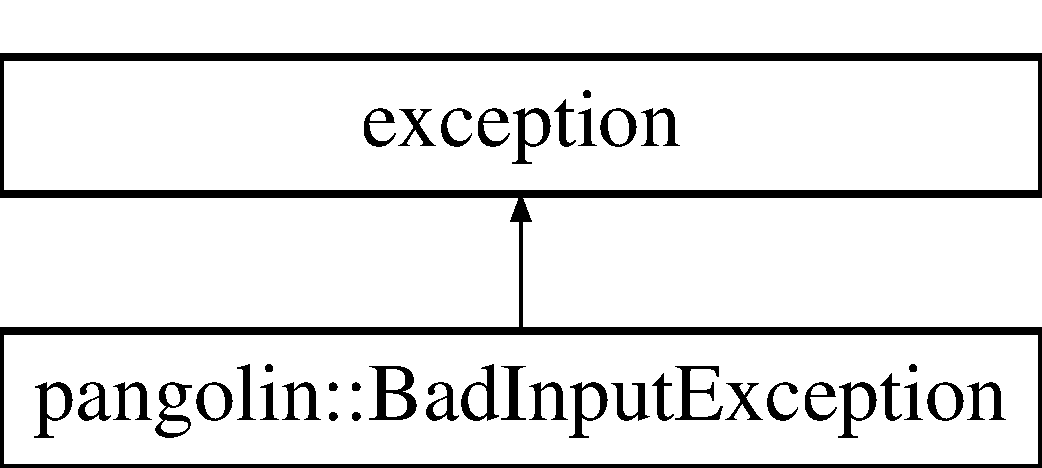
\includegraphics[height=2.000000cm]{structpangolin_1_1_bad_input_exception}
\end{center}
\end{figure}
\subsection*{Public Member Functions}
\begin{DoxyCompactItemize}
\item 
char const $\ast$ {\bfseries what} () const   throw ()\hypertarget{structpangolin_1_1_bad_input_exception_a78f0d2f6e381b900258c8fd161fc6f69}{}\label{structpangolin_1_1_bad_input_exception_a78f0d2f6e381b900258c8fd161fc6f69}

\end{DoxyCompactItemize}


The documentation for this struct was generated from the following file\+:\begin{DoxyCompactItemize}
\item 
/home/gapo/meng/deps/pangolin/include/pangolin/utils/type\+\_\+convert.\+h\end{DoxyCompactItemize}

\hypertarget{structpangolin_1_1buffer}{}\section{pangolin\+:\+:buffer Struct Reference}
\label{structpangolin_1_1buffer}\index{pangolin\+::buffer@{pangolin\+::buffer}}
\subsection*{Public Attributes}
\begin{DoxyCompactItemize}
\item 
void $\ast$ {\bfseries start}\hypertarget{structpangolin_1_1buffer_abec86539d0c4f78804936b34ec1aa80f}{}\label{structpangolin_1_1buffer_abec86539d0c4f78804936b34ec1aa80f}

\item 
size\+\_\+t {\bfseries length}\hypertarget{structpangolin_1_1buffer_a8e7d9dba51b845aa86a9337ae7dd5945}{}\label{structpangolin_1_1buffer_a8e7d9dba51b845aa86a9337ae7dd5945}

\end{DoxyCompactItemize}


The documentation for this struct was generated from the following file\+:\begin{DoxyCompactItemize}
\item 
/home/gapo/meng/deps/pangolin/include/pangolin/video/drivers/v4l.\+h\end{DoxyCompactItemize}

\hypertarget{structpangolin_1_1_button}{}\section{pangolin\+:\+:Button Struct Reference}
\label{structpangolin_1_1_button}\index{pangolin\+::\+Button@{pangolin\+::\+Button}}
Inheritance diagram for pangolin\+:\+:Button\+:\begin{figure}[H]
\begin{center}
\leavevmode
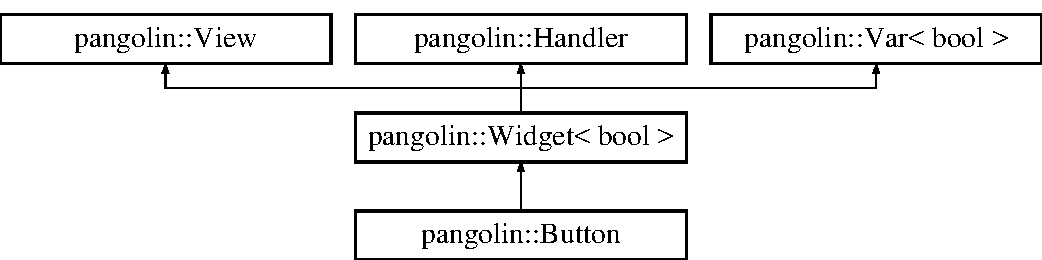
\includegraphics[height=3.000000cm]{structpangolin_1_1_button}
\end{center}
\end{figure}
\subsection*{Public Member Functions}
\begin{DoxyCompactItemize}
\item 
{\bfseries Button} (std\+::string title, \hyperlink{classpangolin_1_1_var_value_generic}{Var\+Value\+Generic} \&tv)\hypertarget{structpangolin_1_1_button_a6986974271cac97ef59d6287581fdbfc}{}\label{structpangolin_1_1_button_a6986974271cac97ef59d6287581fdbfc}

\item 
void {\bfseries Mouse} (\hyperlink{structpangolin_1_1_view}{View} \&, Mouse\+Button button, int x, int y, bool pressed, int mouse\+\_\+state)\hypertarget{structpangolin_1_1_button_a9ce3becafe18a9286c15f812473b23aa}{}\label{structpangolin_1_1_button_a9ce3becafe18a9286c15f812473b23aa}

\item 
void \hyperlink{structpangolin_1_1_button_a567d43e3b445ce6158c21a20c3751190}{Render} ()
\begin{DoxyCompactList}\small\item\em Perform any automatic rendering for this \hyperlink{structpangolin_1_1_view}{View}. \end{DoxyCompactList}\item 
void \hyperlink{structpangolin_1_1_button_a3477cc1ac51e4d0df131febb1341cfd3}{Resize\+Children} ()\hypertarget{structpangolin_1_1_button_a3477cc1ac51e4d0df131febb1341cfd3}{}\label{structpangolin_1_1_button_a3477cc1ac51e4d0df131febb1341cfd3}

\begin{DoxyCompactList}\small\item\em Instruct all children to resize. \end{DoxyCompactList}\end{DoxyCompactItemize}
\subsection*{Public Attributes}
\begin{DoxyCompactItemize}
\item 
\hyperlink{classpangolin_1_1_gl_text}{Gl\+Text} {\bfseries gltext}\hypertarget{structpangolin_1_1_button_a227fa239957d8c12b85a1e9aadedc980}{}\label{structpangolin_1_1_button_a227fa239957d8c12b85a1e9aadedc980}

\item 
G\+Lfloat {\bfseries raster} \mbox{[}2\mbox{]}\hypertarget{structpangolin_1_1_button_a32034c9dfa3adb639f709ccacb45161f}{}\label{structpangolin_1_1_button_a32034c9dfa3adb639f709ccacb45161f}

\item 
bool {\bfseries down}\hypertarget{structpangolin_1_1_button_a190e8414f97e3856c05ed5d47a4329c4}{}\label{structpangolin_1_1_button_a190e8414f97e3856c05ed5d47a4329c4}

\end{DoxyCompactItemize}
\subsection*{Additional Inherited Members}


\subsection{Member Function Documentation}
\index{pangolin\+::\+Button@{pangolin\+::\+Button}!Render@{Render}}
\index{Render@{Render}!pangolin\+::\+Button@{pangolin\+::\+Button}}
\subsubsection[{\texorpdfstring{Render()}{Render()}}]{\setlength{\rightskip}{0pt plus 5cm}void pangolin\+::\+Button\+::\+Render (
\begin{DoxyParamCaption}
{}
\end{DoxyParamCaption}
)\hspace{0.3cm}{\ttfamily [virtual]}}\hypertarget{structpangolin_1_1_button_a567d43e3b445ce6158c21a20c3751190}{}\label{structpangolin_1_1_button_a567d43e3b445ce6158c21a20c3751190}


Perform any automatic rendering for this \hyperlink{structpangolin_1_1_view}{View}. 

Default implementation simply instructs children to render themselves. 

Reimplemented from \hyperlink{structpangolin_1_1_view_a15bf43d7ebc4ebe4e02cba572f0d49ba}{pangolin\+::\+View}.



The documentation for this struct was generated from the following file\+:\begin{DoxyCompactItemize}
\item 
/home/gapo/meng/deps/pangolin/include/pangolin/display/widgets/widgets.\+h\end{DoxyCompactItemize}

\hypertarget{structpangolin_1_1_camera_spec}{}\section{pangolin\+:\+:Camera\+Spec Struct Reference}
\label{structpangolin_1_1_camera_spec}\index{pangolin\+::\+Camera\+Spec@{pangolin\+::\+Camera\+Spec}}
\subsection*{Public Attributes}
\begin{DoxyCompactItemize}
\item 
G\+Lprecision {\bfseries forward} \mbox{[}3\mbox{]}\hypertarget{structpangolin_1_1_camera_spec_a6d79c60d254b53737d3485c3a85b76ef}{}\label{structpangolin_1_1_camera_spec_a6d79c60d254b53737d3485c3a85b76ef}

\item 
G\+Lprecision {\bfseries up} \mbox{[}3\mbox{]}\hypertarget{structpangolin_1_1_camera_spec_a6950692c29299f9aae736c6f75588e62}{}\label{structpangolin_1_1_camera_spec_a6950692c29299f9aae736c6f75588e62}

\item 
G\+Lprecision {\bfseries right} \mbox{[}3\mbox{]}\hypertarget{structpangolin_1_1_camera_spec_a8bc5725f8d8d940f71d661afc6638348}{}\label{structpangolin_1_1_camera_spec_a8bc5725f8d8d940f71d661afc6638348}

\item 
G\+Lprecision {\bfseries img\+\_\+up} \mbox{[}2\mbox{]}\hypertarget{structpangolin_1_1_camera_spec_ac131e80b3ee4e7af9bd166cf970b8fbc}{}\label{structpangolin_1_1_camera_spec_ac131e80b3ee4e7af9bd166cf970b8fbc}

\item 
G\+Lprecision {\bfseries img\+\_\+right} \mbox{[}2\mbox{]}\hypertarget{structpangolin_1_1_camera_spec_abb578352f1f5e3a603dbd8229b002c68}{}\label{structpangolin_1_1_camera_spec_abb578352f1f5e3a603dbd8229b002c68}

\end{DoxyCompactItemize}


The documentation for this struct was generated from the following file\+:\begin{DoxyCompactItemize}
\item 
/home/gapo/meng/deps/pangolin/include/pangolin/display/opengl\+\_\+render\+\_\+state.\+h\end{DoxyCompactItemize}

\hypertarget{classpangolin_1_1_cg_loader}{}\section{pangolin\+:\+:Cg\+Loader Class Reference}
\label{classpangolin_1_1_cg_loader}\index{pangolin\+::\+Cg\+Loader@{pangolin\+::\+Cg\+Loader}}
\subsection*{Public Member Functions}
\begin{DoxyCompactItemize}
\item 
void {\bfseries Initialise} ()\hypertarget{classpangolin_1_1_cg_loader_aa608b30d63f553dcf5de3f07594b348b}{}\label{classpangolin_1_1_cg_loader_aa608b30d63f553dcf5de3f07594b348b}

\item 
\hyperlink{classpangolin_1_1_cg_program}{Cg\+Program} {\bfseries Load\+Program\+From\+File} (const std\+::string \&file, const std\+::string \&function, bool is\+Vertex\+Shader)\hypertarget{classpangolin_1_1_cg_loader_a2a9d37566910c0e8c17091c3cb3d30ec}{}\label{classpangolin_1_1_cg_loader_a2a9d37566910c0e8c17091c3cb3d30ec}

\item 
void {\bfseries Enable\+Program} (\hyperlink{classpangolin_1_1_cg_program}{Cg\+Program} program)\hypertarget{classpangolin_1_1_cg_loader_a693a9d871cfc0f249f7708e3ae58c07c}{}\label{classpangolin_1_1_cg_loader_a693a9d871cfc0f249f7708e3ae58c07c}

\item 
void {\bfseries Disable\+Programs} ()\hypertarget{classpangolin_1_1_cg_loader_a66bb5d130232afb3ac0b7d1448dc1a9a}{}\label{classpangolin_1_1_cg_loader_a66bb5d130232afb3ac0b7d1448dc1a9a}

\item 
void {\bfseries Render\+Dummy\+Quad} ()\hypertarget{classpangolin_1_1_cg_loader_ad728ee64031964ac4ff90d7775c35153}{}\label{classpangolin_1_1_cg_loader_ad728ee64031964ac4ff90d7775c35153}

\item 
void {\bfseries Render\+Dummy\+Quad\+With\+Tex\+Coords} (int w, int h)\hypertarget{classpangolin_1_1_cg_loader_a56bb178a003230640efacefe1d781054}{}\label{classpangolin_1_1_cg_loader_a56bb178a003230640efacefe1d781054}

\end{DoxyCompactItemize}
\subsection*{Protected Attributes}
\begin{DoxyCompactItemize}
\item 
C\+Gcontext {\bfseries m\+Context}\hypertarget{classpangolin_1_1_cg_loader_a3c54d797489644ded7c972ed86729b56}{}\label{classpangolin_1_1_cg_loader_a3c54d797489644ded7c972ed86729b56}

\item 
C\+Gprofile {\bfseries m\+Fragment\+Profile}\hypertarget{classpangolin_1_1_cg_loader_af1e35088663265366c0c5e0d9fcd44a1}{}\label{classpangolin_1_1_cg_loader_af1e35088663265366c0c5e0d9fcd44a1}

\item 
C\+Gprofile {\bfseries m\+Vertex\+Profile}\hypertarget{classpangolin_1_1_cg_loader_ab5510b2ae2a929f107b9111f2b5357fb}{}\label{classpangolin_1_1_cg_loader_ab5510b2ae2a929f107b9111f2b5357fb}

\end{DoxyCompactItemize}


The documentation for this class was generated from the following file\+:\begin{DoxyCompactItemize}
\item 
/home/gapo/meng/deps/pangolin/include/pangolin/gl/cg.\+h\end{DoxyCompactItemize}

\hypertarget{classpangolin_1_1_cg_program}{}\section{pangolin\+:\+:Cg\+Program Class Reference}
\label{classpangolin_1_1_cg_program}\index{pangolin\+::\+Cg\+Program@{pangolin\+::\+Cg\+Program}}


Lightweight object wrapper for N\+Vidia Cg Shader program objects.  




{\ttfamily \#include $<$cg.\+h$>$}

\subsection*{Public Member Functions}
\begin{DoxyCompactItemize}
\item 
void {\bfseries Set\+Uniform} (const std\+::string \&name, \hyperlink{classpangolin_1_1_gl_texture}{Gl\+Texture} \&tex)\hypertarget{classpangolin_1_1_cg_program_a4670a3f84702d074e44b4aecf5ab3cbe}{}\label{classpangolin_1_1_cg_program_a4670a3f84702d074e44b4aecf5ab3cbe}

\item 
void {\bfseries Set\+Uniform} (const std\+::string \&name, float f)\hypertarget{classpangolin_1_1_cg_program_a9dee495f42bafdddd49869f9b43203d2}{}\label{classpangolin_1_1_cg_program_a9dee495f42bafdddd49869f9b43203d2}

\item 
void {\bfseries Update\+Params} ()\hypertarget{classpangolin_1_1_cg_program_ae35a6b434a00f7fc6238e0b0ff6fcc59}{}\label{classpangolin_1_1_cg_program_ae35a6b434a00f7fc6238e0b0ff6fcc59}

\end{DoxyCompactItemize}
\subsection*{Protected Attributes}
\begin{DoxyCompactItemize}
\item 
C\+Gprogram {\bfseries m\+Prog}\hypertarget{classpangolin_1_1_cg_program_a2f690aaf6587a6f4dd535e68ce8f3f0d}{}\label{classpangolin_1_1_cg_program_a2f690aaf6587a6f4dd535e68ce8f3f0d}

\item 
C\+Gcontext {\bfseries m\+Context}\hypertarget{classpangolin_1_1_cg_program_aa315f89e845a24116459e5a2ac8de699}{}\label{classpangolin_1_1_cg_program_aa315f89e845a24116459e5a2ac8de699}

\item 
C\+Gprofile {\bfseries m\+Profile}\hypertarget{classpangolin_1_1_cg_program_ab580ae58de5ad803da1e5b6e6d0e8dd2}{}\label{classpangolin_1_1_cg_program_ab580ae58de5ad803da1e5b6e6d0e8dd2}

\end{DoxyCompactItemize}
\subsection*{Friends}
\begin{DoxyCompactItemize}
\item 
class {\bfseries Cg\+Loader}\hypertarget{classpangolin_1_1_cg_program_a01a9f1198be9776655a9dfab0cfc9f44}{}\label{classpangolin_1_1_cg_program_a01a9f1198be9776655a9dfab0cfc9f44}

\end{DoxyCompactItemize}


\subsection{Detailed Description}
Lightweight object wrapper for N\+Vidia Cg Shader program objects. 

The documentation for this class was generated from the following file\+:\begin{DoxyCompactItemize}
\item 
/home/gapo/meng/deps/pangolin/include/pangolin/gl/cg.\+h\end{DoxyCompactItemize}

\hypertarget{structpangolin_1_1_checkbox}{}\section{pangolin\+:\+:Checkbox Struct Reference}
\label{structpangolin_1_1_checkbox}\index{pangolin\+::\+Checkbox@{pangolin\+::\+Checkbox}}
Inheritance diagram for pangolin\+:\+:Checkbox\+:\begin{figure}[H]
\begin{center}
\leavevmode
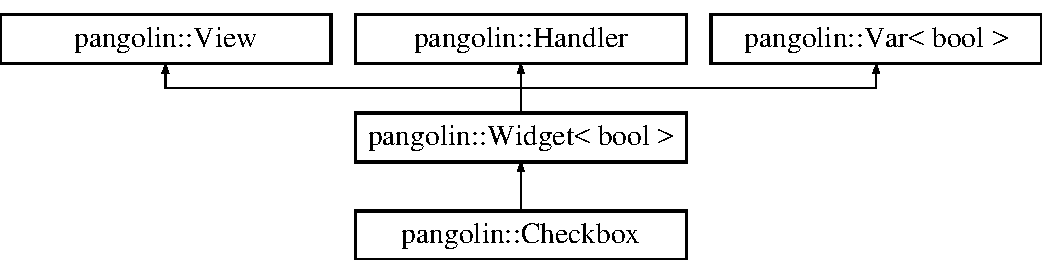
\includegraphics[height=3.000000cm]{structpangolin_1_1_checkbox}
\end{center}
\end{figure}
\subsection*{Public Member Functions}
\begin{DoxyCompactItemize}
\item 
{\bfseries Checkbox} (std\+::string title, \hyperlink{classpangolin_1_1_var_value_generic}{Var\+Value\+Generic} \&tv)\hypertarget{structpangolin_1_1_checkbox_a774a603e8eb3504ecfdc3b91a03274be}{}\label{structpangolin_1_1_checkbox_a774a603e8eb3504ecfdc3b91a03274be}

\item 
void {\bfseries Mouse} (\hyperlink{structpangolin_1_1_view}{View} \&, Mouse\+Button button, int x, int y, bool pressed, int mouse\+\_\+state)\hypertarget{structpangolin_1_1_checkbox_a565837d74e7e09121fbda5b12a5b210d}{}\label{structpangolin_1_1_checkbox_a565837d74e7e09121fbda5b12a5b210d}

\item 
void \hyperlink{structpangolin_1_1_checkbox_aa6e9cf9fd2a35b06e0a6462ccd50747d}{Render} ()
\begin{DoxyCompactList}\small\item\em Perform any automatic rendering for this \hyperlink{structpangolin_1_1_view}{View}. \end{DoxyCompactList}\item 
void \hyperlink{structpangolin_1_1_checkbox_a05c067eb4d3e7f7b95dab56c63768b01}{Resize\+Children} ()\hypertarget{structpangolin_1_1_checkbox_a05c067eb4d3e7f7b95dab56c63768b01}{}\label{structpangolin_1_1_checkbox_a05c067eb4d3e7f7b95dab56c63768b01}

\begin{DoxyCompactList}\small\item\em Instruct all children to resize. \end{DoxyCompactList}\end{DoxyCompactItemize}
\subsection*{Public Attributes}
\begin{DoxyCompactItemize}
\item 
\hyperlink{classpangolin_1_1_gl_text}{Gl\+Text} {\bfseries gltext}\hypertarget{structpangolin_1_1_checkbox_aac61c9efef58aa6e93df0c7f6dbec775}{}\label{structpangolin_1_1_checkbox_aac61c9efef58aa6e93df0c7f6dbec775}

\item 
G\+Lfloat {\bfseries raster} \mbox{[}2\mbox{]}\hypertarget{structpangolin_1_1_checkbox_aaced624dcb0f0831acd859accbfff118}{}\label{structpangolin_1_1_checkbox_aaced624dcb0f0831acd859accbfff118}

\item 
\hyperlink{structpangolin_1_1_viewport}{Viewport} {\bfseries vcb}\hypertarget{structpangolin_1_1_checkbox_a3a65fc63633d19d0737c084f196a8703}{}\label{structpangolin_1_1_checkbox_a3a65fc63633d19d0737c084f196a8703}

\end{DoxyCompactItemize}
\subsection*{Additional Inherited Members}


\subsection{Member Function Documentation}
\index{pangolin\+::\+Checkbox@{pangolin\+::\+Checkbox}!Render@{Render}}
\index{Render@{Render}!pangolin\+::\+Checkbox@{pangolin\+::\+Checkbox}}
\subsubsection[{\texorpdfstring{Render()}{Render()}}]{\setlength{\rightskip}{0pt plus 5cm}void pangolin\+::\+Checkbox\+::\+Render (
\begin{DoxyParamCaption}
{}
\end{DoxyParamCaption}
)\hspace{0.3cm}{\ttfamily [virtual]}}\hypertarget{structpangolin_1_1_checkbox_aa6e9cf9fd2a35b06e0a6462ccd50747d}{}\label{structpangolin_1_1_checkbox_aa6e9cf9fd2a35b06e0a6462ccd50747d}


Perform any automatic rendering for this \hyperlink{structpangolin_1_1_view}{View}. 

Default implementation simply instructs children to render themselves. 

Reimplemented from \hyperlink{structpangolin_1_1_view_a15bf43d7ebc4ebe4e02cba572f0d49ba}{pangolin\+::\+View}.



The documentation for this struct was generated from the following file\+:\begin{DoxyCompactItemize}
\item 
/home/gapo/meng/deps/pangolin/include/pangolin/display/widgets/widgets.\+h\end{DoxyCompactItemize}

\hypertarget{structpangolin_1_1_colour}{}\section{pangolin\+:\+:Colour Struct Reference}
\label{structpangolin_1_1_colour}\index{pangolin\+::\+Colour@{pangolin\+::\+Colour}}


Represent Open\+GL floating point colour\+: Red, Green and Blue with alpha.  




{\ttfamily \#include $<$colour.\+h$>$}

\subsection*{Public Member Functions}
\begin{DoxyCompactItemize}
\item 
\hyperlink{structpangolin_1_1_colour_af104120f620167f683d7eaa02924e70b}{Colour} ()\hypertarget{structpangolin_1_1_colour_af104120f620167f683d7eaa02924e70b}{}\label{structpangolin_1_1_colour_af104120f620167f683d7eaa02924e70b}

\begin{DoxyCompactList}\small\item\em Default constructs white. \end{DoxyCompactList}\item 
\hyperlink{structpangolin_1_1_colour_a8f2a64fe74d5048185450333526edaef}{Colour} (float red, float green, float blue, float alpha=1.\+0)\hypertarget{structpangolin_1_1_colour_a8f2a64fe74d5048185450333526edaef}{}\label{structpangolin_1_1_colour_a8f2a64fe74d5048185450333526edaef}

\begin{DoxyCompactList}\small\item\em Construct from component values. \end{DoxyCompactList}\item 
\hyperlink{structpangolin_1_1_colour_aad7b39a22043478cade30fa1a07958ed}{Colour} (float rgba\mbox{[}4\mbox{]})\hypertarget{structpangolin_1_1_colour_aad7b39a22043478cade30fa1a07958ed}{}\label{structpangolin_1_1_colour_aad7b39a22043478cade30fa1a07958ed}

\begin{DoxyCompactList}\small\item\em Construct from rgba array. \end{DoxyCompactList}\item 
float $\ast$ \hyperlink{structpangolin_1_1_colour_aba37f36802ae8559ba79188b8e5c7832}{Get} ()\hypertarget{structpangolin_1_1_colour_aba37f36802ae8559ba79188b8e5c7832}{}\label{structpangolin_1_1_colour_aba37f36802ae8559ba79188b8e5c7832}

\begin{DoxyCompactList}\small\item\em Return pointer to Open\+GL compatible R\+G\+BA array. \end{DoxyCompactList}\item 
\hyperlink{structpangolin_1_1_colour}{Colour} \hyperlink{structpangolin_1_1_colour_ae5405e31317ec5b65a205072f58a3b1a}{With\+Alpha} (float alpha)\hypertarget{structpangolin_1_1_colour_ae5405e31317ec5b65a205072f58a3b1a}{}\label{structpangolin_1_1_colour_ae5405e31317ec5b65a205072f58a3b1a}

\begin{DoxyCompactList}\small\item\em Return this colour with alpha adjusted. \end{DoxyCompactList}\end{DoxyCompactItemize}
\subsection*{Static Public Member Functions}
\begin{DoxyCompactItemize}
\item 
static \hyperlink{structpangolin_1_1_colour}{Colour} \hyperlink{structpangolin_1_1_colour_a52eef9b76740ae72099e5e2e4ca5f980}{Hsv} (float hue, float sat=1.\+0, float val=1.\+0, float alpha=1.\+0)
\begin{DoxyCompactList}\small\item\em Construct from H\+SV \hyperlink{structpangolin_1_1_colour}{Colour}. \end{DoxyCompactList}\end{DoxyCompactItemize}
\subsection*{Public Attributes}
\begin{DoxyCompactItemize}
\item 
\begin{tabbing}
xx\=xx\=xx\=xx\=xx\=xx\=xx\=xx\=xx\=\kill
union \{\\
\>struct \{\\
\>\>float {\bfseries red}\\
\>\>float {\bfseries green}\\
\>\>float {\bfseries blue}\\
\>\>float {\bfseries alpha}\\
\>\} \hypertarget{unionpangolin_1_1_colour_1_1_0D2_ac14aaf73fa8a358f8058cfbcb2d05fd2}{}\label{unionpangolin_1_1_colour_1_1_0D2_ac14aaf73fa8a358f8058cfbcb2d05fd2}
\\
\>struct \{\\
\>\>float {\bfseries r}\\
\>\>float {\bfseries g}\\
\>\>float {\bfseries b}\\
\>\>float {\bfseries a}\\
\>\} \hypertarget{unionpangolin_1_1_colour_1_1_0D2_a160340ce5224aabe94ae3477e41a540e}{}\label{unionpangolin_1_1_colour_1_1_0D2_a160340ce5224aabe94ae3477e41a540e}
\\
\>float {\bfseries c} \mbox{[}4\mbox{]}\\
\}; \hypertarget{structpangolin_1_1_colour_a4054bd432b1a1774b709474ca99a21c1}{}\label{structpangolin_1_1_colour_a4054bd432b1a1774b709474ca99a21c1}
\\

\end{tabbing}\end{DoxyCompactItemize}


\subsection{Detailed Description}
Represent Open\+GL floating point colour\+: Red, Green and Blue with alpha. 

\subsection{Member Function Documentation}
\index{pangolin\+::\+Colour@{pangolin\+::\+Colour}!Hsv@{Hsv}}
\index{Hsv@{Hsv}!pangolin\+::\+Colour@{pangolin\+::\+Colour}}
\subsubsection[{\texorpdfstring{Hsv(float hue, float sat=1.\+0, float val=1.\+0, float alpha=1.\+0)}{Hsv(float hue, float sat=1.0, float val=1.0, float alpha=1.0)}}]{\setlength{\rightskip}{0pt plus 5cm}static {\bf Colour} pangolin\+::\+Colour\+::\+Hsv (
\begin{DoxyParamCaption}
\item[{float}]{hue, }
\item[{float}]{sat = {\ttfamily 1.0}, }
\item[{float}]{val = {\ttfamily 1.0}, }
\item[{float}]{alpha = {\ttfamily 1.0}}
\end{DoxyParamCaption}
)\hspace{0.3cm}{\ttfamily [inline]}, {\ttfamily [static]}}\hypertarget{structpangolin_1_1_colour_a52eef9b76740ae72099e5e2e4ca5f980}{}\label{structpangolin_1_1_colour_a52eef9b76740ae72099e5e2e4ca5f980}


Construct from H\+SV \hyperlink{structpangolin_1_1_colour}{Colour}. 


\begin{DoxyParams}{Parameters}
{\em hue} & \hyperlink{structpangolin_1_1_colour}{Colour} hue in range \mbox{[}0,1\mbox{]} \\
\hline
{\em sat} & Saturation in range \mbox{[}0,1\mbox{]} \\
\hline
{\em val} & Value / Brightness in range \mbox{[}0,1\mbox{]}. \\
\hline
\end{DoxyParams}


The documentation for this struct was generated from the following file\+:\begin{DoxyCompactItemize}
\item 
/home/gapo/meng/deps/pangolin/include/pangolin/gl/colour.\+h\end{DoxyCompactItemize}

\hypertarget{classpangolin_1_1_colour_wheel}{}\section{pangolin\+:\+:Colour\+Wheel Class Reference}
\label{classpangolin_1_1_colour_wheel}\index{pangolin\+::\+Colour\+Wheel@{pangolin\+::\+Colour\+Wheel}}


A \hyperlink{classpangolin_1_1_colour_wheel}{Colour\+Wheel} is like a continuous colour palate that can be sampled.  




{\ttfamily \#include $<$colour.\+h$>$}

\subsection*{Public Member Functions}
\begin{DoxyCompactItemize}
\item 
\hyperlink{classpangolin_1_1_colour_wheel_a3ceb3513ba6cad92d6e2844671da7f43}{Colour\+Wheel} (float saturation=0.\+5, float value=1.\+0, float alpha=1.\+0)\hypertarget{classpangolin_1_1_colour_wheel_a3ceb3513ba6cad92d6e2844671da7f43}{}\label{classpangolin_1_1_colour_wheel_a3ceb3513ba6cad92d6e2844671da7f43}

\begin{DoxyCompactList}\small\item\em Construct \hyperlink{classpangolin_1_1_colour_wheel}{Colour\+Wheel} with Saturation, Value and Alpha constant. \end{DoxyCompactList}\item 
\hyperlink{structpangolin_1_1_colour}{Colour} \hyperlink{classpangolin_1_1_colour_wheel_ac8d1538dbe99eca9eb769f3a6076ea53}{Get\+Colour\+Bin} (int i) const \hypertarget{classpangolin_1_1_colour_wheel_ac8d1538dbe99eca9eb769f3a6076ea53}{}\label{classpangolin_1_1_colour_wheel_ac8d1538dbe99eca9eb769f3a6076ea53}

\begin{DoxyCompactList}\small\item\em Use Golden ratio (/angle) to pick well spaced colours. \end{DoxyCompactList}\item 
\hyperlink{structpangolin_1_1_colour}{Colour} \hyperlink{classpangolin_1_1_colour_wheel_af6f84ad1b063c82019927fee17ceba3f}{Get\+Unique\+Colour} ()\hypertarget{classpangolin_1_1_colour_wheel_af6f84ad1b063c82019927fee17ceba3f}{}\label{classpangolin_1_1_colour_wheel_af6f84ad1b063c82019927fee17ceba3f}

\begin{DoxyCompactList}\small\item\em Return next unique colour from \hyperlink{classpangolin_1_1_colour_wheel}{Colour\+Wheel}. \end{DoxyCompactList}\end{DoxyCompactItemize}
\subsection*{Protected Attributes}
\begin{DoxyCompactItemize}
\item 
int {\bfseries unique\+\_\+colours}\hypertarget{classpangolin_1_1_colour_wheel_a7829fb1c01b8f0f3b93ad7436892a92f}{}\label{classpangolin_1_1_colour_wheel_a7829fb1c01b8f0f3b93ad7436892a92f}

\item 
float {\bfseries sat}\hypertarget{classpangolin_1_1_colour_wheel_a4c7188ac25ce50b5b77038668c1b4b73}{}\label{classpangolin_1_1_colour_wheel_a4c7188ac25ce50b5b77038668c1b4b73}

\item 
float {\bfseries val}\hypertarget{classpangolin_1_1_colour_wheel_a2e1f6a24f74dd33eb0a67b503cd63e8a}{}\label{classpangolin_1_1_colour_wheel_a2e1f6a24f74dd33eb0a67b503cd63e8a}

\item 
float {\bfseries alpha}\hypertarget{classpangolin_1_1_colour_wheel_a73efd17611316d61e992f2095fcbbcb5}{}\label{classpangolin_1_1_colour_wheel_a73efd17611316d61e992f2095fcbbcb5}

\end{DoxyCompactItemize}


\subsection{Detailed Description}
A \hyperlink{classpangolin_1_1_colour_wheel}{Colour\+Wheel} is like a continuous colour palate that can be sampled. 

In the future, different Colour\+Wheels will be supported, but this one is based on sampling hues in H\+SV colourspace. An indefinite number of unique colours are sampled using the golden angle. 

The documentation for this class was generated from the following file\+:\begin{DoxyCompactItemize}
\item 
/home/gapo/meng/deps/pangolin/include/pangolin/gl/colour.\+h\end{DoxyCompactItemize}

\hypertarget{classpangolin_1_1_console_interpreter}{}\section{pangolin\+:\+:Console\+Interpreter Class Reference}
\label{classpangolin_1_1_console_interpreter}\index{pangolin\+::\+Console\+Interpreter@{pangolin\+::\+Console\+Interpreter}}
Inheritance diagram for pangolin\+:\+:Console\+Interpreter\+:\begin{figure}[H]
\begin{center}
\leavevmode
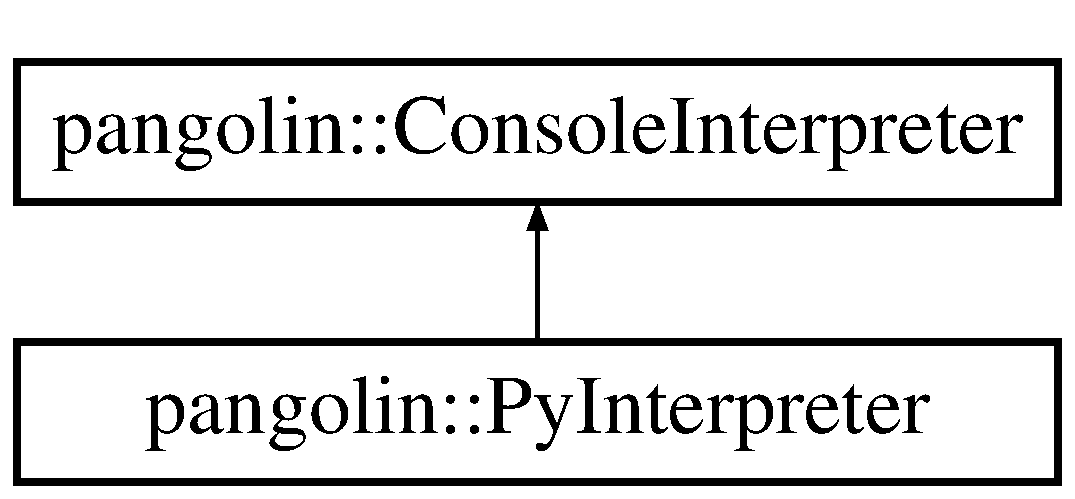
\includegraphics[height=2.000000cm]{classpangolin_1_1_console_interpreter}
\end{center}
\end{figure}
\subsection*{Public Member Functions}
\begin{DoxyCompactItemize}
\item 
virtual void {\bfseries Push\+Command} (const std\+::string \&cmd)=0\hypertarget{classpangolin_1_1_console_interpreter_a2e7c382a0ae3bcc8d8dd155664f41ece}{}\label{classpangolin_1_1_console_interpreter_a2e7c382a0ae3bcc8d8dd155664f41ece}

\item 
virtual bool {\bfseries Pull\+Line} (\hyperlink{classpangolin_1_1_console_line}{Console\+Line} \&line)=0\hypertarget{classpangolin_1_1_console_interpreter_a9241290da4e778dede19de5c9b8de3c0}{}\label{classpangolin_1_1_console_interpreter_a9241290da4e778dede19de5c9b8de3c0}

\item 
virtual std\+::vector$<$ std\+::string $>$ {\bfseries Complete} (const std\+::string \&cmd, int max\+\_\+options=20)=0\hypertarget{classpangolin_1_1_console_interpreter_addab1784c137ff32d8d48d3488db9d8b}{}\label{classpangolin_1_1_console_interpreter_addab1784c137ff32d8d48d3488db9d8b}

\end{DoxyCompactItemize}


The documentation for this class was generated from the following file\+:\begin{DoxyCompactItemize}
\item 
/home/gapo/meng/deps/pangolin/include/pangolin/console/Console\+Interpreter.\+h\end{DoxyCompactItemize}

\hypertarget{classpangolin_1_1_console_line}{}\section{pangolin\+:\+:Console\+Line Class Reference}
\label{classpangolin_1_1_console_line}\index{pangolin\+::\+Console\+Line@{pangolin\+::\+Console\+Line}}
\subsection*{Public Member Functions}
\begin{DoxyCompactItemize}
\item 
{\bfseries Console\+Line} (std\+::string text, Console\+Line\+Type linetype=Console\+Line\+Type\+Output)\hypertarget{classpangolin_1_1_console_line_afb729b09fb44b866e430a02667874b27}{}\label{classpangolin_1_1_console_line_afb729b09fb44b866e430a02667874b27}

\end{DoxyCompactItemize}
\subsection*{Public Attributes}
\begin{DoxyCompactItemize}
\item 
std\+::string {\bfseries text}\hypertarget{classpangolin_1_1_console_line_a617b481c9c6e61c582b661900996338c}{}\label{classpangolin_1_1_console_line_a617b481c9c6e61c582b661900996338c}

\item 
Console\+Line\+Type {\bfseries linetype}\hypertarget{classpangolin_1_1_console_line_a17d9cd91ec915bf78eb56316fe736c4e}{}\label{classpangolin_1_1_console_line_a17d9cd91ec915bf78eb56316fe736c4e}

\end{DoxyCompactItemize}


The documentation for this class was generated from the following file\+:\begin{DoxyCompactItemize}
\item 
/home/gapo/meng/deps/pangolin/include/pangolin/console/Console\+Interpreter.\+h\end{DoxyCompactItemize}

\hypertarget{classpangolin_1_1_console_view}{}\section{pangolin\+:\+:Console\+View Class Reference}
\label{classpangolin_1_1_console_view}\index{pangolin\+::\+Console\+View@{pangolin\+::\+Console\+View}}
Inheritance diagram for pangolin\+:\+:Console\+View\+:\begin{figure}[H]
\begin{center}
\leavevmode
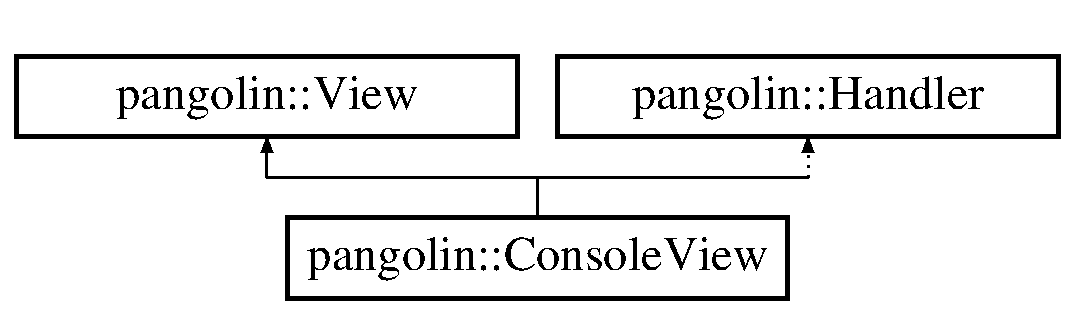
\includegraphics[height=2.000000cm]{classpangolin_1_1_console_view}
\end{center}
\end{figure}
\subsection*{Classes}
\begin{DoxyCompactItemize}
\item 
struct \hyperlink{structpangolin_1_1_console_view_1_1_line}{Line}
\end{DoxyCompactItemize}
\subsection*{Public Member Functions}
\begin{DoxyCompactItemize}
\item 
{\bfseries Console\+View} (\hyperlink{classpangolin_1_1_console_interpreter}{Console\+Interpreter} $\ast$interpreter)\hypertarget{classpangolin_1_1_console_view_a699259931f9e06c42c483abd9b1d1fce}{}\label{classpangolin_1_1_console_view_a699259931f9e06c42c483abd9b1d1fce}

\item 
\hyperlink{structpangolin_1_1_view}{View} \& {\bfseries Show} (bool show=true)\hypertarget{classpangolin_1_1_console_view_a3c0b4f5f43fe090758bda243c980b188}{}\label{classpangolin_1_1_console_view_a3c0b4f5f43fe090758bda243c980b188}

\item 
void {\bfseries Toggle\+Show} ()\hypertarget{classpangolin_1_1_console_view_a8546a64ea3592ddd39c5fbcc62ac2a7d}{}\label{classpangolin_1_1_console_view_a8546a64ea3592ddd39c5fbcc62ac2a7d}

\item 
bool {\bfseries Is\+Shown} () const \hypertarget{classpangolin_1_1_console_view_a098860c962a94c6e95331087c31dc4c5}{}\label{classpangolin_1_1_console_view_a098860c962a94c6e95331087c31dc4c5}

\item 
void \hyperlink{classpangolin_1_1_console_view_aca9edf0d08cfc5bb028464379797a908}{Render} () P\+A\+N\+G\+O\+L\+I\+N\+\_\+\+O\+V\+E\+R\+R\+I\+DE
\begin{DoxyCompactList}\small\item\em Perform any automatic rendering for this \hyperlink{structpangolin_1_1_view}{View}. \end{DoxyCompactList}\item 
void {\bfseries Keyboard} (\hyperlink{structpangolin_1_1_view}{View} \&, unsigned char key, int x, int y, bool pressed) P\+A\+N\+G\+O\+L\+I\+N\+\_\+\+O\+V\+E\+R\+R\+I\+DE\hypertarget{classpangolin_1_1_console_view_abbc01c957ef410d5c788d0d146cace79}{}\label{classpangolin_1_1_console_view_abbc01c957ef410d5c788d0d146cace79}

\end{DoxyCompactItemize}
\subsection*{Additional Inherited Members}


\subsection{Member Function Documentation}
\index{pangolin\+::\+Console\+View@{pangolin\+::\+Console\+View}!Render@{Render}}
\index{Render@{Render}!pangolin\+::\+Console\+View@{pangolin\+::\+Console\+View}}
\subsubsection[{\texorpdfstring{Render() P\+A\+N\+G\+O\+L\+I\+N\+\_\+\+O\+V\+E\+R\+R\+I\+DE}{Render() PANGOLIN_OVERRIDE}}]{\setlength{\rightskip}{0pt plus 5cm}void pangolin\+::\+Console\+View\+::\+Render (
\begin{DoxyParamCaption}
{}
\end{DoxyParamCaption}
)\hspace{0.3cm}{\ttfamily [virtual]}}\hypertarget{classpangolin_1_1_console_view_aca9edf0d08cfc5bb028464379797a908}{}\label{classpangolin_1_1_console_view_aca9edf0d08cfc5bb028464379797a908}


Perform any automatic rendering for this \hyperlink{structpangolin_1_1_view}{View}. 

Default implementation simply instructs children to render themselves. 

Reimplemented from \hyperlink{structpangolin_1_1_view_a15bf43d7ebc4ebe4e02cba572f0d49ba}{pangolin\+::\+View}.



The documentation for this class was generated from the following file\+:\begin{DoxyCompactItemize}
\item 
/home/gapo/meng/deps/pangolin/include/pangolin/console/Console\+View.\+h\end{DoxyCompactItemize}

\hypertarget{structpangolin_1_1_convert}{}\section{pangolin\+:\+:Convert$<$ T, S, Enable $>$ Struct Template Reference}
\label{structpangolin_1_1_convert}\index{pangolin\+::\+Convert$<$ T, S, Enable $>$@{pangolin\+::\+Convert$<$ T, S, Enable $>$}}
\subsection*{Static Public Member Functions}
\begin{DoxyCompactItemize}
\item 
static T {\bfseries Do} (const S \&src)\hypertarget{structpangolin_1_1_convert_af2bf0fbbcf0674f51954fa0a2974f89d}{}\label{structpangolin_1_1_convert_af2bf0fbbcf0674f51954fa0a2974f89d}

\end{DoxyCompactItemize}


The documentation for this struct was generated from the following file\+:\begin{DoxyCompactItemize}
\item 
/home/gapo/meng/deps/pangolin/include/pangolin/utils/type\+\_\+convert.\+h\end{DoxyCompactItemize}

\hypertarget{structpangolin_1_1_convert_3_01bool_00_01std_1_1string_01_4}{}\section{pangolin\+:\+:Convert$<$ bool, std\+:\+:string $>$ Struct Template Reference}
\label{structpangolin_1_1_convert_3_01bool_00_01std_1_1string_01_4}\index{pangolin\+::\+Convert$<$ bool, std\+::string $>$@{pangolin\+::\+Convert$<$ bool, std\+::string $>$}}
\subsection*{Static Public Member Functions}
\begin{DoxyCompactItemize}
\item 
static bool {\bfseries Do} (const std\+::string \&src)\hypertarget{structpangolin_1_1_convert_3_01bool_00_01std_1_1string_01_4_aba02f14cc321725404c8585ba65ff94d}{}\label{structpangolin_1_1_convert_3_01bool_00_01std_1_1string_01_4_aba02f14cc321725404c8585ba65ff94d}

\end{DoxyCompactItemize}


The documentation for this struct was generated from the following file\+:\begin{DoxyCompactItemize}
\item 
/home/gapo/meng/deps/pangolin/include/pangolin/utils/type\+\_\+convert.\+h\end{DoxyCompactItemize}

\hypertarget{structpangolin_1_1_convert_3_01std_1_1string_00_01_s_00_01typename_01pangolin_1_1enable__if__c_3664d08d7238157e37db033a565859915}{}\section{pangolin\+:\+:Convert$<$ std\+:\+:string, S, typename pangolin\+:\+:enable\+\_\+if\+\_\+c$<$ !boostd\+:\+:is\+\_\+same$<$ S, std\+:\+:string $>$\+:\+:value $>$\+:\+:type $>$ Struct Template Reference}
\label{structpangolin_1_1_convert_3_01std_1_1string_00_01_s_00_01typename_01pangolin_1_1enable__if__c_3664d08d7238157e37db033a565859915}\index{pangolin\+::\+Convert$<$ std\+::string, S, typename pangolin\+::enable\+\_\+if\+\_\+c$<$ "!boostd\+::is\+\_\+same$<$ S, std\+::string $>$\+::value $>$\+::type $>$@{pangolin\+::\+Convert$<$ std\+::string, S, typename pangolin\+::enable\+\_\+if\+\_\+c$<$ "!boostd\+::is\+\_\+same$<$ S, std\+::string $>$\+::value $>$\+::type $>$}}
\subsection*{Static Public Member Functions}
\begin{DoxyCompactItemize}
\item 
static std\+::string {\bfseries Do} (const S \&src)\hypertarget{structpangolin_1_1_convert_3_01std_1_1string_00_01_s_00_01typename_01pangolin_1_1enable__if__c_3664d08d7238157e37db033a565859915_adb20284b06426daf9ff05c84a684a6ed}{}\label{structpangolin_1_1_convert_3_01std_1_1string_00_01_s_00_01typename_01pangolin_1_1enable__if__c_3664d08d7238157e37db033a565859915_adb20284b06426daf9ff05c84a684a6ed}

\end{DoxyCompactItemize}


The documentation for this struct was generated from the following file\+:\begin{DoxyCompactItemize}
\item 
/home/gapo/meng/deps/pangolin/include/pangolin/utils/type\+\_\+convert.\+h\end{DoxyCompactItemize}

\hypertarget{structpangolin_1_1_convert_3_01_t_00_01_s_00_01typename_01pangolin_1_1enable__if__c_3_01boostd_14fa16b198ae7b6f1e4cb0a8f7ff718eb}{}\section{pangolin\+:\+:Convert$<$ T, S, typename pangolin\+:\+:enable\+\_\+if\+\_\+c$<$ boostd\+:\+:is\+\_\+same$<$ T, bool $>$\+:\+:value \&\&boostd\+:\+:is\+\_\+scalar$<$ S $>$\+:\+:value \&\&!boostd\+:\+:is\+\_\+same$<$ S, T $>$\+:\+:value $>$\+:\+:type $>$ Struct Template Reference}
\label{structpangolin_1_1_convert_3_01_t_00_01_s_00_01typename_01pangolin_1_1enable__if__c_3_01boostd_14fa16b198ae7b6f1e4cb0a8f7ff718eb}\index{pangolin\+::\+Convert$<$ T, S, typename pangolin\+::enable\+\_\+if\+\_\+c$<$ boostd\+::is\+\_\+same$<$ T, bool $>$\+::value \&\&boostd\+::is\+\_\+scalar$<$ S $>$\+::value \&\&"!boostd\+::is\+\_\+same$<$ S, T $>$\+::value $>$\+::type $>$@{pangolin\+::\+Convert$<$ T, S, typename pangolin\+::enable\+\_\+if\+\_\+c$<$ boostd\+::is\+\_\+same$<$ T, bool $>$\+::value \&\&boostd\+::is\+\_\+scalar$<$ S $>$\+::value \&\&"!boostd\+::is\+\_\+same$<$ S, T $>$\+::value $>$\+::type $>$}}
\subsection*{Static Public Member Functions}
\begin{DoxyCompactItemize}
\item 
static T {\bfseries Do} (const S \&src)\hypertarget{structpangolin_1_1_convert_3_01_t_00_01_s_00_01typename_01pangolin_1_1enable__if__c_3_01boostd_14fa16b198ae7b6f1e4cb0a8f7ff718eb_ab9dede8d154cb446b95e1edc8c2284a4}{}\label{structpangolin_1_1_convert_3_01_t_00_01_s_00_01typename_01pangolin_1_1enable__if__c_3_01boostd_14fa16b198ae7b6f1e4cb0a8f7ff718eb_ab9dede8d154cb446b95e1edc8c2284a4}

\end{DoxyCompactItemize}


The documentation for this struct was generated from the following file\+:\begin{DoxyCompactItemize}
\item 
/home/gapo/meng/deps/pangolin/include/pangolin/utils/type\+\_\+convert.\+h\end{DoxyCompactItemize}

\hypertarget{structpangolin_1_1_convert_3_01_t_00_01_s_00_01typename_01pangolin_1_1enable__if__c_3_01boostd_15bb04e576c082ab636857abc71178db4}{}\section{pangolin\+:\+:Convert$<$ T, S, typename pangolin\+:\+:enable\+\_\+if\+\_\+c$<$ boostd\+:\+:is\+\_\+scalar$<$ T $>$\+:\+:value \&\&!boostd\+:\+:is\+\_\+same$<$ T, bool $>$\+:\+:value \&\&boostd\+:\+:is\+\_\+scalar$<$ S $>$\+:\+:value \&\&!boostd\+:\+:is\+\_\+same$<$ S, bool $>$\+:\+:value \&\&!boostd\+:\+:is\+\_\+same$<$ S, T $>$\+:\+:value $>$\+:\+:type $>$ Struct Template Reference}
\label{structpangolin_1_1_convert_3_01_t_00_01_s_00_01typename_01pangolin_1_1enable__if__c_3_01boostd_15bb04e576c082ab636857abc71178db4}\index{pangolin\+::\+Convert$<$ T, S, typename pangolin\+::enable\+\_\+if\+\_\+c$<$ boostd\+::is\+\_\+scalar$<$ T $>$\+::value \&\&"!boostd\+::is\+\_\+same$<$ T, bool $>$\+::value \&\&boostd\+::is\+\_\+scalar$<$ S $>$\+::value \&\&"!boostd\+::is\+\_\+same$<$ S, bool $>$\+::value \&\&"!boostd\+::is\+\_\+same$<$ S, T $>$\+::value $>$\+::type $>$@{pangolin\+::\+Convert$<$ T, S, typename pangolin\+::enable\+\_\+if\+\_\+c$<$ boostd\+::is\+\_\+scalar$<$ T $>$\+::value \&\&"!boostd\+::is\+\_\+same$<$ T, bool $>$\+::value \&\&boostd\+::is\+\_\+scalar$<$ S $>$\+::value \&\&"!boostd\+::is\+\_\+same$<$ S, bool $>$\+::value \&\&"!boostd\+::is\+\_\+same$<$ S, T $>$\+::value $>$\+::type $>$}}
\subsection*{Static Public Member Functions}
\begin{DoxyCompactItemize}
\item 
static T {\bfseries Do} (const S \&src)\hypertarget{structpangolin_1_1_convert_3_01_t_00_01_s_00_01typename_01pangolin_1_1enable__if__c_3_01boostd_15bb04e576c082ab636857abc71178db4_a8972f65a05af676f29c83038f7016c4a}{}\label{structpangolin_1_1_convert_3_01_t_00_01_s_00_01typename_01pangolin_1_1enable__if__c_3_01boostd_15bb04e576c082ab636857abc71178db4_a8972f65a05af676f29c83038f7016c4a}

\end{DoxyCompactItemize}


The documentation for this struct was generated from the following file\+:\begin{DoxyCompactItemize}
\item 
/home/gapo/meng/deps/pangolin/include/pangolin/utils/type\+\_\+convert.\+h\end{DoxyCompactItemize}

\hypertarget{structpangolin_1_1_convert_3_01_t_00_01_s_00_01typename_01pangolin_1_1enable__if__c_3_01boostd_199ff7ea2c1912b7457b88f7ead1b4239}{}\section{pangolin\+:\+:Convert$<$ T, S, typename pangolin\+:\+:enable\+\_\+if\+\_\+c$<$ boostd\+:\+:is\+\_\+scalar$<$ T $>$\+:\+:value \&\&boostd\+:\+:is\+\_\+same$<$ S, bool $>$\+:\+:value \&\&!boostd\+:\+:is\+\_\+same$<$ S, T $>$\+:\+:value $>$\+:\+:type $>$ Struct Template Reference}
\label{structpangolin_1_1_convert_3_01_t_00_01_s_00_01typename_01pangolin_1_1enable__if__c_3_01boostd_199ff7ea2c1912b7457b88f7ead1b4239}\index{pangolin\+::\+Convert$<$ T, S, typename pangolin\+::enable\+\_\+if\+\_\+c$<$ boostd\+::is\+\_\+scalar$<$ T $>$\+::value \&\&boostd\+::is\+\_\+same$<$ S, bool $>$\+::value \&\&"!boostd\+::is\+\_\+same$<$ S, T $>$\+::value $>$\+::type $>$@{pangolin\+::\+Convert$<$ T, S, typename pangolin\+::enable\+\_\+if\+\_\+c$<$ boostd\+::is\+\_\+scalar$<$ T $>$\+::value \&\&boostd\+::is\+\_\+same$<$ S, bool $>$\+::value \&\&"!boostd\+::is\+\_\+same$<$ S, T $>$\+::value $>$\+::type $>$}}
\subsection*{Static Public Member Functions}
\begin{DoxyCompactItemize}
\item 
static T {\bfseries Do} (const S \&src)\hypertarget{structpangolin_1_1_convert_3_01_t_00_01_s_00_01typename_01pangolin_1_1enable__if__c_3_01boostd_199ff7ea2c1912b7457b88f7ead1b4239_a45308ee5f160c3740a792cbebd966be2}{}\label{structpangolin_1_1_convert_3_01_t_00_01_s_00_01typename_01pangolin_1_1enable__if__c_3_01boostd_199ff7ea2c1912b7457b88f7ead1b4239_a45308ee5f160c3740a792cbebd966be2}

\end{DoxyCompactItemize}


The documentation for this struct was generated from the following file\+:\begin{DoxyCompactItemize}
\item 
/home/gapo/meng/deps/pangolin/include/pangolin/utils/type\+\_\+convert.\+h\end{DoxyCompactItemize}

\hypertarget{structpangolin_1_1_convert_3_01_t_00_01std_1_1string_00_01typename_01pangolin_1_1enable__if__c_3e41c835b953ae45734366e409b5e4a53}{}\section{pangolin\+:\+:Convert$<$ T, std\+:\+:string, typename pangolin\+:\+:enable\+\_\+if\+\_\+c$<$ !boostd\+:\+:is\+\_\+same$<$ T, std\+:\+:string $>$\+:\+:value $>$\+:\+:type $>$ Struct Template Reference}
\label{structpangolin_1_1_convert_3_01_t_00_01std_1_1string_00_01typename_01pangolin_1_1enable__if__c_3e41c835b953ae45734366e409b5e4a53}\index{pangolin\+::\+Convert$<$ T, std\+::string, typename pangolin\+::enable\+\_\+if\+\_\+c$<$ "!boostd\+::is\+\_\+same$<$ T, std\+::string $>$\+::value $>$\+::type $>$@{pangolin\+::\+Convert$<$ T, std\+::string, typename pangolin\+::enable\+\_\+if\+\_\+c$<$ "!boostd\+::is\+\_\+same$<$ T, std\+::string $>$\+::value $>$\+::type $>$}}
\subsection*{Static Public Member Functions}
\begin{DoxyCompactItemize}
\item 
static T {\bfseries Do} (const std\+::string \&src)\hypertarget{structpangolin_1_1_convert_3_01_t_00_01std_1_1string_00_01typename_01pangolin_1_1enable__if__c_3e41c835b953ae45734366e409b5e4a53_a688918fe5783fa4c0e2c1abe70fdd967}{}\label{structpangolin_1_1_convert_3_01_t_00_01std_1_1string_00_01typename_01pangolin_1_1enable__if__c_3e41c835b953ae45734366e409b5e4a53_a688918fe5783fa4c0e2c1abe70fdd967}

\end{DoxyCompactItemize}


The documentation for this struct was generated from the following file\+:\begin{DoxyCompactItemize}
\item 
/home/gapo/meng/deps/pangolin/include/pangolin/utils/type\+\_\+convert.\+h\end{DoxyCompactItemize}

\hypertarget{structpangolin_1_1_convert_3_01_t_00_01_t_01_4}{}\section{pangolin\+:\+:Convert$<$ T, T $>$ Struct Template Reference}
\label{structpangolin_1_1_convert_3_01_t_00_01_t_01_4}\index{pangolin\+::\+Convert$<$ T, T $>$@{pangolin\+::\+Convert$<$ T, T $>$}}
\subsection*{Static Public Member Functions}
\begin{DoxyCompactItemize}
\item 
static T {\bfseries Do} (const T \&src)\hypertarget{structpangolin_1_1_convert_3_01_t_00_01_t_01_4_afc02e0a0f4b2a192103a209b602aa602}{}\label{structpangolin_1_1_convert_3_01_t_00_01_t_01_4_afc02e0a0f4b2a192103a209b602aa602}

\end{DoxyCompactItemize}


The documentation for this struct was generated from the following file\+:\begin{DoxyCompactItemize}
\item 
/home/gapo/meng/deps/pangolin/include/pangolin/utils/type\+\_\+convert.\+h\end{DoxyCompactItemize}

\hypertarget{structpangolin_1_1_cuda_scoped_mapped_array}{}\section{pangolin\+:\+:Cuda\+Scoped\+Mapped\+Array Struct Reference}
\label{structpangolin_1_1_cuda_scoped_mapped_array}\index{pangolin\+::\+Cuda\+Scoped\+Mapped\+Array@{pangolin\+::\+Cuda\+Scoped\+Mapped\+Array}}
\subsection*{Public Member Functions}
\begin{DoxyCompactItemize}
\item 
{\bfseries Cuda\+Scoped\+Mapped\+Array} (\hyperlink{structpangolin_1_1_gl_texture_cuda_array}{Gl\+Texture\+Cuda\+Array} \&tex)\hypertarget{structpangolin_1_1_cuda_scoped_mapped_array_a5e475af1a93717dd89eb23978954c972}{}\label{structpangolin_1_1_cuda_scoped_mapped_array_a5e475af1a93717dd89eb23978954c972}

\item 
cuda\+Array $\ast$ {\bfseries operator$\ast$} ()\hypertarget{structpangolin_1_1_cuda_scoped_mapped_array_a4c2bb5b010b9f73388e6f9c6e818534d}{}\label{structpangolin_1_1_cuda_scoped_mapped_array_a4c2bb5b010b9f73388e6f9c6e818534d}

\end{DoxyCompactItemize}
\subsection*{Public Attributes}
\begin{DoxyCompactItemize}
\item 
cuda\+Graphics\+Resource $\ast$ {\bfseries res}\hypertarget{structpangolin_1_1_cuda_scoped_mapped_array_a660beb8a542d1943b61b50d441a501ef}{}\label{structpangolin_1_1_cuda_scoped_mapped_array_a660beb8a542d1943b61b50d441a501ef}

\end{DoxyCompactItemize}


The documentation for this struct was generated from the following file\+:\begin{DoxyCompactItemize}
\item 
/home/gapo/meng/deps/pangolin/include/pangolin/gl/glcuda.\+h\end{DoxyCompactItemize}

\hypertarget{structpangolin_1_1_cuda_scoped_mapped_ptr}{}\section{pangolin\+:\+:Cuda\+Scoped\+Mapped\+Ptr Struct Reference}
\label{structpangolin_1_1_cuda_scoped_mapped_ptr}\index{pangolin\+::\+Cuda\+Scoped\+Mapped\+Ptr@{pangolin\+::\+Cuda\+Scoped\+Mapped\+Ptr}}
\subsection*{Public Member Functions}
\begin{DoxyCompactItemize}
\item 
{\bfseries Cuda\+Scoped\+Mapped\+Ptr} (\hyperlink{structpangolin_1_1_gl_buffer_cuda_ptr}{Gl\+Buffer\+Cuda\+Ptr} \&\hyperlink{structpangolin_1_1buffer}{buffer})\hypertarget{structpangolin_1_1_cuda_scoped_mapped_ptr_ad79e228449c3e70fe2142098f6963749}{}\label{structpangolin_1_1_cuda_scoped_mapped_ptr_ad79e228449c3e70fe2142098f6963749}

\item 
void $\ast$ {\bfseries operator$\ast$} ()\hypertarget{structpangolin_1_1_cuda_scoped_mapped_ptr_a42b1c4536e3ad0d9e58631879ade5f60}{}\label{structpangolin_1_1_cuda_scoped_mapped_ptr_a42b1c4536e3ad0d9e58631879ade5f60}

\end{DoxyCompactItemize}
\subsection*{Public Attributes}
\begin{DoxyCompactItemize}
\item 
cuda\+Graphics\+Resource $\ast$ {\bfseries res}\hypertarget{structpangolin_1_1_cuda_scoped_mapped_ptr_a964c6366fdffe0430b3f41b9c1b31504}{}\label{structpangolin_1_1_cuda_scoped_mapped_ptr_a964c6366fdffe0430b3f41b9c1b31504}

\end{DoxyCompactItemize}


The documentation for this struct was generated from the following file\+:\begin{DoxyCompactItemize}
\item 
/home/gapo/meng/deps/pangolin/include/pangolin/gl/glcuda.\+h\end{DoxyCompactItemize}

\hypertarget{classpangolin_1_1_data_log}{}\section{pangolin\+:\+:Data\+Log Class Reference}
\label{classpangolin_1_1_data_log}\index{pangolin\+::\+Data\+Log@{pangolin\+::\+Data\+Log}}


A \hyperlink{classpangolin_1_1_data_log}{Data\+Log} can efficiently record floating point sample data of any size.  




{\ttfamily \#include $<$datalog.\+h$>$}

\subsection*{Public Member Functions}
\begin{DoxyCompactItemize}
\item 
\hyperlink{classpangolin_1_1_data_log_a0c8f4f1670198d8a3ea316871d6fb44a}{Data\+Log} (unsigned int block\+\_\+samples\+\_\+alloc=10000)
\item 
void \hyperlink{classpangolin_1_1_data_log_aa7eb0e27c58460dd5392158f9ead6d3b}{Set\+Labels} (const std\+::vector$<$ std\+::string $>$ \&labels)
\begin{DoxyCompactList}\small\item\em Provide textual labels corresponding to each dimension logged. \end{DoxyCompactList}\item 
const std\+::vector$<$ std\+::string $>$ \& {\bfseries Labels} () const \hypertarget{classpangolin_1_1_data_log_a7f82e7854a40fe48eca912a4fdc3fd3c}{}\label{classpangolin_1_1_data_log_a7f82e7854a40fe48eca912a4fdc3fd3c}

\item 
void {\bfseries Log} (unsigned int dimension, const float $\ast$vals, unsigned int samples=1)\hypertarget{classpangolin_1_1_data_log_a8e18b177f25638e0bc5bbbadd6869ac3}{}\label{classpangolin_1_1_data_log_a8e18b177f25638e0bc5bbbadd6869ac3}

\item 
void {\bfseries Log} (float v)\hypertarget{classpangolin_1_1_data_log_ac3514c098e2fd0831ccfca5800cf4de7}{}\label{classpangolin_1_1_data_log_ac3514c098e2fd0831ccfca5800cf4de7}

\item 
void {\bfseries Log} (float v1, float v2)\hypertarget{classpangolin_1_1_data_log_aba33eb426fe42c9eebe9db5df756eab2}{}\label{classpangolin_1_1_data_log_aba33eb426fe42c9eebe9db5df756eab2}

\item 
void {\bfseries Log} (float v1, float v2, float v3)\hypertarget{classpangolin_1_1_data_log_a239375ed52092dc34df73f9769bb8916}{}\label{classpangolin_1_1_data_log_a239375ed52092dc34df73f9769bb8916}

\item 
void {\bfseries Log} (float v1, float v2, float v3, float v4)\hypertarget{classpangolin_1_1_data_log_a8b5655beb52a0bfefcd5f1cad7740471}{}\label{classpangolin_1_1_data_log_a8b5655beb52a0bfefcd5f1cad7740471}

\item 
void {\bfseries Log} (float v1, float v2, float v3, float v4, float v5)\hypertarget{classpangolin_1_1_data_log_a3e5bb5245f7ace74d1edfe22cf3caca2}{}\label{classpangolin_1_1_data_log_a3e5bb5245f7ace74d1edfe22cf3caca2}

\item 
void {\bfseries Log} (float v1, float v2, float v3, float v4, float v5, float v6)\hypertarget{classpangolin_1_1_data_log_af777f6a6ad712a2c661fc46dc5116134}{}\label{classpangolin_1_1_data_log_af777f6a6ad712a2c661fc46dc5116134}

\item 
void {\bfseries Log} (float v1, float v2, float v3, float v4, float v5, float v6, float v7)\hypertarget{classpangolin_1_1_data_log_a7911073c03725fe4e16210cd9dc1a7f7}{}\label{classpangolin_1_1_data_log_a7911073c03725fe4e16210cd9dc1a7f7}

\item 
void {\bfseries Log} (float v1, float v2, float v3, float v4, float v5, float v6, float v7, float v8)\hypertarget{classpangolin_1_1_data_log_aeb93b51a7205c3e9075932e8bb085520}{}\label{classpangolin_1_1_data_log_aeb93b51a7205c3e9075932e8bb085520}

\item 
void {\bfseries Log} (float v1, float v2, float v3, float v4, float v5, float v6, float v7, float v8, float v9)\hypertarget{classpangolin_1_1_data_log_afd4d65ada2542407964fcb5546127eb0}{}\label{classpangolin_1_1_data_log_afd4d65ada2542407964fcb5546127eb0}

\item 
void {\bfseries Log} (float v1, float v2, float v3, float v4, float v5, float v6, float v7, float v8, float v9, float v10)\hypertarget{classpangolin_1_1_data_log_aa4e904fcf838d2d1985eafcd5b34dd9a}{}\label{classpangolin_1_1_data_log_aa4e904fcf838d2d1985eafcd5b34dd9a}

\item 
void {\bfseries Log} (const std\+::vector$<$ float $>$ \&vals)\hypertarget{classpangolin_1_1_data_log_a93f2055a18e59137d36d662e96436565}{}\label{classpangolin_1_1_data_log_a93f2055a18e59137d36d662e96436565}

\item 
void {\bfseries Clear} ()\hypertarget{classpangolin_1_1_data_log_a6c7507f95ee9f73a266ea1ffa4aaecbb}{}\label{classpangolin_1_1_data_log_a6c7507f95ee9f73a266ea1ffa4aaecbb}

\item 
void {\bfseries Save} (std\+::string filename)\hypertarget{classpangolin_1_1_data_log_ade4c0071631ef20172906a50279026a2}{}\label{classpangolin_1_1_data_log_ade4c0071631ef20172906a50279026a2}

\item 
const \hyperlink{classpangolin_1_1_data_log_block}{Data\+Log\+Block} $\ast$ {\bfseries First\+Block} () const \hypertarget{classpangolin_1_1_data_log_a8304ddf3c98448431798a12521c6c690}{}\label{classpangolin_1_1_data_log_a8304ddf3c98448431798a12521c6c690}

\item 
const \hyperlink{classpangolin_1_1_data_log_block}{Data\+Log\+Block} $\ast$ {\bfseries Last\+Block} () const \hypertarget{classpangolin_1_1_data_log_ab7c456328a50f2e196fbf47cc77aa67c}{}\label{classpangolin_1_1_data_log_ab7c456328a50f2e196fbf47cc77aa67c}

\item 
unsigned int {\bfseries Samples} () const \hypertarget{classpangolin_1_1_data_log_a125e32c0ee4767f72253d8a544741c92}{}\label{classpangolin_1_1_data_log_a125e32c0ee4767f72253d8a544741c92}

\item 
const float $\ast$ {\bfseries Sample} (int n) const \hypertarget{classpangolin_1_1_data_log_a99538f491bbf39f78712025d4218dff4}{}\label{classpangolin_1_1_data_log_a99538f491bbf39f78712025d4218dff4}

\item 
const \hyperlink{structpangolin_1_1_dimension_stats}{Dimension\+Stats} \& {\bfseries Stats} (size\+\_\+t dim) const \hypertarget{classpangolin_1_1_data_log_ac51716574725c8aa0cf3d1705c134ad4}{}\label{classpangolin_1_1_data_log_ac51716574725c8aa0cf3d1705c134ad4}

\end{DoxyCompactItemize}
\subsection*{Protected Attributes}
\begin{DoxyCompactItemize}
\item 
unsigned int {\bfseries block\+\_\+samples\+\_\+alloc}\hypertarget{classpangolin_1_1_data_log_a990a2d63bd18bd4c4cdf96cc8a4602ba}{}\label{classpangolin_1_1_data_log_a990a2d63bd18bd4c4cdf96cc8a4602ba}

\item 
std\+::vector$<$ std\+::string $>$ {\bfseries labels}\hypertarget{classpangolin_1_1_data_log_a17b9968806d9251ddd6cbf204e9ca4c0}{}\label{classpangolin_1_1_data_log_a17b9968806d9251ddd6cbf204e9ca4c0}

\item 
\hyperlink{classpangolin_1_1_data_log_block}{Data\+Log\+Block} $\ast$ {\bfseries block0}\hypertarget{classpangolin_1_1_data_log_a618cec617dc2b8405729abb7889c3179}{}\label{classpangolin_1_1_data_log_a618cec617dc2b8405729abb7889c3179}

\item 
\hyperlink{classpangolin_1_1_data_log_block}{Data\+Log\+Block} $\ast$ {\bfseries blockn}\hypertarget{classpangolin_1_1_data_log_ad8ab0338adf86fc912d6211a3502155d}{}\label{classpangolin_1_1_data_log_ad8ab0338adf86fc912d6211a3502155d}

\item 
std\+::vector$<$ \hyperlink{structpangolin_1_1_dimension_stats}{Dimension\+Stats} $>$ {\bfseries stats}\hypertarget{classpangolin_1_1_data_log_a0b31a1be6ccba4ecb465e48a2cf18fef}{}\label{classpangolin_1_1_data_log_a0b31a1be6ccba4ecb465e48a2cf18fef}

\item 
bool {\bfseries record\+\_\+stats}\hypertarget{classpangolin_1_1_data_log_a989503f87d8b8e452d517c1ec7b7ab8f}{}\label{classpangolin_1_1_data_log_a989503f87d8b8e452d517c1ec7b7ab8f}

\end{DoxyCompactItemize}


\subsection{Detailed Description}
A \hyperlink{classpangolin_1_1_data_log}{Data\+Log} can efficiently record floating point sample data of any size. 

Memory is allocated in blocks is transparent to the user. 

\subsection{Constructor \& Destructor Documentation}
\index{pangolin\+::\+Data\+Log@{pangolin\+::\+Data\+Log}!Data\+Log@{Data\+Log}}
\index{Data\+Log@{Data\+Log}!pangolin\+::\+Data\+Log@{pangolin\+::\+Data\+Log}}
\subsubsection[{\texorpdfstring{Data\+Log(unsigned int block\+\_\+samples\+\_\+alloc=10000)}{DataLog(unsigned int block_samples_alloc=10000)}}]{\setlength{\rightskip}{0pt plus 5cm}pangolin\+::\+Data\+Log\+::\+Data\+Log (
\begin{DoxyParamCaption}
\item[{unsigned int}]{block\+\_\+samples\+\_\+alloc = {\ttfamily 10000}}
\end{DoxyParamCaption}
)}\hypertarget{classpangolin_1_1_data_log_a0c8f4f1670198d8a3ea316871d6fb44a}{}\label{classpangolin_1_1_data_log_a0c8f4f1670198d8a3ea316871d6fb44a}

\begin{DoxyParams}{Parameters}
{\em block\+\_\+samples\+\_\+alloc} & number of samples each memory block can hold. \\
\hline
\end{DoxyParams}


\subsection{Member Function Documentation}
\index{pangolin\+::\+Data\+Log@{pangolin\+::\+Data\+Log}!Set\+Labels@{Set\+Labels}}
\index{Set\+Labels@{Set\+Labels}!pangolin\+::\+Data\+Log@{pangolin\+::\+Data\+Log}}
\subsubsection[{\texorpdfstring{Set\+Labels(const std\+::vector$<$ std\+::string $>$ \&labels)}{SetLabels(const std::vector< std::string > &labels)}}]{\setlength{\rightskip}{0pt plus 5cm}void pangolin\+::\+Data\+Log\+::\+Set\+Labels (
\begin{DoxyParamCaption}
\item[{const std\+::vector$<$ std\+::string $>$ \&}]{labels}
\end{DoxyParamCaption}
)}\hypertarget{classpangolin_1_1_data_log_aa7eb0e27c58460dd5392158f9ead6d3b}{}\label{classpangolin_1_1_data_log_aa7eb0e27c58460dd5392158f9ead6d3b}


Provide textual labels corresponding to each dimension logged. 

This information may be used by graphical interfaces to \hyperlink{classpangolin_1_1_data_log}{Data\+Log}. 

The documentation for this class was generated from the following file\+:\begin{DoxyCompactItemize}
\item 
/home/gapo/meng/deps/pangolin/include/pangolin/plot/datalog.\+h\end{DoxyCompactItemize}

\hypertarget{classpangolin_1_1_data_log_block}{}\section{pangolin\+:\+:Data\+Log\+Block Class Reference}
\label{classpangolin_1_1_data_log_block}\index{pangolin\+::\+Data\+Log\+Block@{pangolin\+::\+Data\+Log\+Block}}
\subsection*{Public Member Functions}
\begin{DoxyCompactItemize}
\item 
\hyperlink{classpangolin_1_1_data_log_block_aede09d66acd9ec8ce26b17d9a9681358}{Data\+Log\+Block} (size\+\_\+t dim, size\+\_\+t max\+\_\+samples, size\+\_\+t start\+\_\+id)
\item 
size\+\_\+t {\bfseries Samples} () const \hypertarget{classpangolin_1_1_data_log_block_ac81f01afbbe07de9a41059fc5a332b05}{}\label{classpangolin_1_1_data_log_block_ac81f01afbbe07de9a41059fc5a332b05}

\item 
size\+\_\+t {\bfseries Max\+Samples} () const \hypertarget{classpangolin_1_1_data_log_block_a448c0dcf93ba8c6a15ede17482534031}{}\label{classpangolin_1_1_data_log_block_a448c0dcf93ba8c6a15ede17482534031}

\item 
size\+\_\+t \hyperlink{classpangolin_1_1_data_log_block_a9f70cb83e4530154536e2551b498f803}{Sample\+Space\+Left} () const \hypertarget{classpangolin_1_1_data_log_block_a9f70cb83e4530154536e2551b498f803}{}\label{classpangolin_1_1_data_log_block_a9f70cb83e4530154536e2551b498f803}

\begin{DoxyCompactList}\small\item\em Return how many more samples can fit in this block. \end{DoxyCompactList}\item 
bool {\bfseries Is\+Full} () const \hypertarget{classpangolin_1_1_data_log_block_a6be29f2cbd2b85ee41c15a9fc86c4552}{}\label{classpangolin_1_1_data_log_block_a6be29f2cbd2b85ee41c15a9fc86c4552}

\item 
void \hyperlink{classpangolin_1_1_data_log_block_aefa329a9eb3c00bc047d9c01beec02b3}{Add\+Samples} (size\+\_\+t num\+\_\+samples, size\+\_\+t dimensions, const float $\ast$data\+\_\+dim\+\_\+major)\hypertarget{classpangolin_1_1_data_log_block_aefa329a9eb3c00bc047d9c01beec02b3}{}\label{classpangolin_1_1_data_log_block_aefa329a9eb3c00bc047d9c01beec02b3}

\begin{DoxyCompactList}\small\item\em Add data to block. \end{DoxyCompactList}\item 
void \hyperlink{classpangolin_1_1_data_log_block_abd0be65d936d41d16724e28a41061f6d}{Clear\+Linked} ()\hypertarget{classpangolin_1_1_data_log_block_abd0be65d936d41d16724e28a41061f6d}{}\label{classpangolin_1_1_data_log_block_abd0be65d936d41d16724e28a41061f6d}

\begin{DoxyCompactList}\small\item\em Delete all samples. \end{DoxyCompactList}\item 
\hyperlink{classpangolin_1_1_data_log_block}{Data\+Log\+Block} $\ast$ {\bfseries Next\+Block} () const \hypertarget{classpangolin_1_1_data_log_block_ab5af4ebb6c68038e5e9482ead3d82d62}{}\label{classpangolin_1_1_data_log_block_ab5af4ebb6c68038e5e9482ead3d82d62}

\item 
size\+\_\+t {\bfseries Start\+Id} () const \hypertarget{classpangolin_1_1_data_log_block_a4cdb1a482d339a6bef91ecf798d29bf3}{}\label{classpangolin_1_1_data_log_block_a4cdb1a482d339a6bef91ecf798d29bf3}

\item 
float $\ast$ {\bfseries Dim\+Data} (size\+\_\+t d) const \hypertarget{classpangolin_1_1_data_log_block_a5aaa212eb3b07023d2fef34530050a13}{}\label{classpangolin_1_1_data_log_block_a5aaa212eb3b07023d2fef34530050a13}

\item 
size\+\_\+t {\bfseries Dimensions} () const \hypertarget{classpangolin_1_1_data_log_block_a17ebf052dae867915b21a60240b7b699}{}\label{classpangolin_1_1_data_log_block_a17ebf052dae867915b21a60240b7b699}

\item 
const float $\ast$ {\bfseries Sample} (size\+\_\+t n) const \hypertarget{classpangolin_1_1_data_log_block_afec77a511bbeaafa4c32c28d85b8f221}{}\label{classpangolin_1_1_data_log_block_afec77a511bbeaafa4c32c28d85b8f221}

\end{DoxyCompactItemize}
\subsection*{Protected Attributes}
\begin{DoxyCompactItemize}
\item 
size\+\_\+t {\bfseries dim}\hypertarget{classpangolin_1_1_data_log_block_a1d098a02ae3ec17fe90cb621fd4003e8}{}\label{classpangolin_1_1_data_log_block_a1d098a02ae3ec17fe90cb621fd4003e8}

\item 
size\+\_\+t {\bfseries max\+\_\+samples}\hypertarget{classpangolin_1_1_data_log_block_a38dad18e71d4db9c7ddc48a3c03d2945}{}\label{classpangolin_1_1_data_log_block_a38dad18e71d4db9c7ddc48a3c03d2945}

\item 
size\+\_\+t {\bfseries samples}\hypertarget{classpangolin_1_1_data_log_block_aadeb0e8a72bca6d4b55bbb384504ff4a}{}\label{classpangolin_1_1_data_log_block_aadeb0e8a72bca6d4b55bbb384504ff4a}

\item 
size\+\_\+t {\bfseries start\+\_\+id}\hypertarget{classpangolin_1_1_data_log_block_a1a33a2d17044257c0ec1963c2ac51bb9}{}\label{classpangolin_1_1_data_log_block_a1a33a2d17044257c0ec1963c2ac51bb9}

\item 
float $\ast$ {\bfseries sample\+\_\+buffer}\hypertarget{classpangolin_1_1_data_log_block_a6731923f4fa4e50b105a1a9efd1fa653}{}\label{classpangolin_1_1_data_log_block_a6731923f4fa4e50b105a1a9efd1fa653}

\item 
\hyperlink{classpangolin_1_1_data_log_block}{Data\+Log\+Block} $\ast$ {\bfseries next\+Block}\hypertarget{classpangolin_1_1_data_log_block_a7e41bf680dc8f525d94dad4434588521}{}\label{classpangolin_1_1_data_log_block_a7e41bf680dc8f525d94dad4434588521}

\end{DoxyCompactItemize}


\subsection{Constructor \& Destructor Documentation}
\index{pangolin\+::\+Data\+Log\+Block@{pangolin\+::\+Data\+Log\+Block}!Data\+Log\+Block@{Data\+Log\+Block}}
\index{Data\+Log\+Block@{Data\+Log\+Block}!pangolin\+::\+Data\+Log\+Block@{pangolin\+::\+Data\+Log\+Block}}
\subsubsection[{\texorpdfstring{Data\+Log\+Block(size\+\_\+t dim, size\+\_\+t max\+\_\+samples, size\+\_\+t start\+\_\+id)}{DataLogBlock(size_t dim, size_t max_samples, size_t start_id)}}]{\setlength{\rightskip}{0pt plus 5cm}pangolin\+::\+Data\+Log\+Block\+::\+Data\+Log\+Block (
\begin{DoxyParamCaption}
\item[{size\+\_\+t}]{dim, }
\item[{size\+\_\+t}]{max\+\_\+samples, }
\item[{size\+\_\+t}]{start\+\_\+id}
\end{DoxyParamCaption}
)\hspace{0.3cm}{\ttfamily [inline]}}\hypertarget{classpangolin_1_1_data_log_block_aede09d66acd9ec8ce26b17d9a9681358}{}\label{classpangolin_1_1_data_log_block_aede09d66acd9ec8ce26b17d9a9681358}

\begin{DoxyParams}{Parameters}
{\em dim} & dimension of sample \\
\hline
{\em max\+\_\+samples} & maximum number of samples this block can hold \\
\hline
{\em start\+\_\+id} & index of first sample (from entire dataset) in this buffer \\
\hline
\end{DoxyParams}


The documentation for this class was generated from the following file\+:\begin{DoxyCompactItemize}
\item 
/home/gapo/meng/deps/pangolin/include/pangolin/plot/datalog.\+h\end{DoxyCompactItemize}

\hypertarget{classpangolin_1_1_debayer_video}{}\section{pangolin\+:\+:Debayer\+Video Class Reference}
\label{classpangolin_1_1_debayer_video}\index{pangolin\+::\+Debayer\+Video@{pangolin\+::\+Debayer\+Video}}
Inheritance diagram for pangolin\+:\+:Debayer\+Video\+:\begin{figure}[H]
\begin{center}
\leavevmode
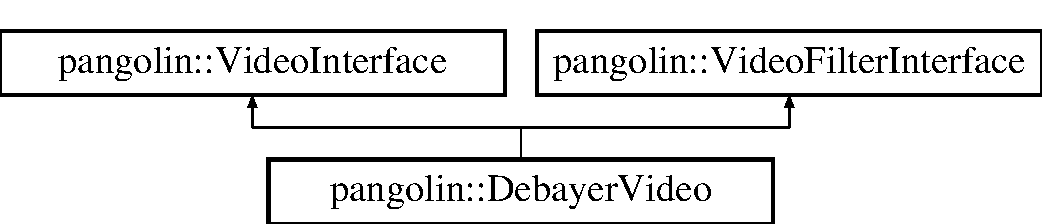
\includegraphics[height=2.000000cm]{classpangolin_1_1_debayer_video}
\end{center}
\end{figure}
\subsection*{Public Member Functions}
\begin{DoxyCompactItemize}
\item 
{\bfseries Debayer\+Video} (\hyperlink{structpangolin_1_1_video_interface}{Video\+Interface} $\ast$videoin, color\+\_\+filter\+\_\+t tile, bayer\+\_\+method\+\_\+t method)\hypertarget{classpangolin_1_1_debayer_video_a56ab8559cc057ab0ea448b4e91dc326c}{}\label{classpangolin_1_1_debayer_video_a56ab8559cc057ab0ea448b4e91dc326c}

\item 
void \hyperlink{classpangolin_1_1_debayer_video_aa294683b7bad6e7ae287bac4c36bbc9a}{Start} ()\hypertarget{classpangolin_1_1_debayer_video_aa294683b7bad6e7ae287bac4c36bbc9a}{}\label{classpangolin_1_1_debayer_video_aa294683b7bad6e7ae287bac4c36bbc9a}

\begin{DoxyCompactList}\small\item\em Implement \hyperlink{structpangolin_1_1_video_input_a74a2e3e1b87c7cbf9de9bcb39e1df128}{Video\+Input\+::\+Start()} \end{DoxyCompactList}\item 
void \hyperlink{classpangolin_1_1_debayer_video_a8406e1f4468ba0a66a70731d2f1caf30}{Stop} ()\hypertarget{classpangolin_1_1_debayer_video_a8406e1f4468ba0a66a70731d2f1caf30}{}\label{classpangolin_1_1_debayer_video_a8406e1f4468ba0a66a70731d2f1caf30}

\begin{DoxyCompactList}\small\item\em Implement \hyperlink{structpangolin_1_1_video_input_a8945f80194cc7ec9594db7f27e7d09b8}{Video\+Input\+::\+Stop()} \end{DoxyCompactList}\item 
size\+\_\+t \hyperlink{classpangolin_1_1_debayer_video_aea059c5ce2046b2ec7f2d5f4594b954c}{Size\+Bytes} () const \hypertarget{classpangolin_1_1_debayer_video_aea059c5ce2046b2ec7f2d5f4594b954c}{}\label{classpangolin_1_1_debayer_video_aea059c5ce2046b2ec7f2d5f4594b954c}

\begin{DoxyCompactList}\small\item\em Implement \hyperlink{structpangolin_1_1_video_input_a93cee5c33386973a2a51165e6bdcf40b}{Video\+Input\+::\+Size\+Bytes()} \end{DoxyCompactList}\item 
const std\+::vector$<$ \hyperlink{classpangolin_1_1_stream_info}{Stream\+Info} $>$ \& \hyperlink{classpangolin_1_1_debayer_video_a0afaf3bf703bdb1e6f76cfad6d94ecad}{Streams} () const \hypertarget{classpangolin_1_1_debayer_video_a0afaf3bf703bdb1e6f76cfad6d94ecad}{}\label{classpangolin_1_1_debayer_video_a0afaf3bf703bdb1e6f76cfad6d94ecad}

\begin{DoxyCompactList}\small\item\em Implement \hyperlink{structpangolin_1_1_video_input_a9030d775d699c39ab7b7ba378c007c6a}{Video\+Input\+::\+Streams()} \end{DoxyCompactList}\item 
bool \hyperlink{classpangolin_1_1_debayer_video_a7d8a25a6a000062b2e8a0bae7c01d280}{Grab\+Next} (unsigned char $\ast$image, bool wait=true)\hypertarget{classpangolin_1_1_debayer_video_a7d8a25a6a000062b2e8a0bae7c01d280}{}\label{classpangolin_1_1_debayer_video_a7d8a25a6a000062b2e8a0bae7c01d280}

\begin{DoxyCompactList}\small\item\em Implement \hyperlink{structpangolin_1_1_video_input_ad3d8ff59c1ec4139320097e6e1111f32}{Video\+Input\+::\+Grab\+Next()} \end{DoxyCompactList}\item 
bool \hyperlink{classpangolin_1_1_debayer_video_ac40d7ecaecde6ecf5fadbecabe73fead}{Grab\+Newest} (unsigned char $\ast$image, bool wait=true)\hypertarget{classpangolin_1_1_debayer_video_ac40d7ecaecde6ecf5fadbecabe73fead}{}\label{classpangolin_1_1_debayer_video_ac40d7ecaecde6ecf5fadbecabe73fead}

\begin{DoxyCompactList}\small\item\em Implement \hyperlink{structpangolin_1_1_video_input_a4c8ac38e3c6a3f591663aeebf645e4c6}{Video\+Input\+::\+Grab\+Newest()} \end{DoxyCompactList}\item 
std\+::vector$<$ \hyperlink{structpangolin_1_1_video_interface}{Video\+Interface} $\ast$ $>$ \& {\bfseries Input\+Streams} ()\hypertarget{classpangolin_1_1_debayer_video_ae449f64f8545bd3e68df380536d9b089}{}\label{classpangolin_1_1_debayer_video_ae449f64f8545bd3e68df380536d9b089}

\end{DoxyCompactItemize}
\subsection*{Protected Attributes}
\begin{DoxyCompactItemize}
\item 
std\+::vector$<$ \hyperlink{structpangolin_1_1_video_interface}{Video\+Interface} $\ast$ $>$ {\bfseries videoin}\hypertarget{classpangolin_1_1_debayer_video_aa342097d0d232e96c1fee8b234248ee8}{}\label{classpangolin_1_1_debayer_video_aa342097d0d232e96c1fee8b234248ee8}

\item 
std\+::vector$<$ \hyperlink{classpangolin_1_1_stream_info}{Stream\+Info} $>$ {\bfseries streams}\hypertarget{classpangolin_1_1_debayer_video_ad03742068d5994ca83b4a182adbd1b81}{}\label{classpangolin_1_1_debayer_video_ad03742068d5994ca83b4a182adbd1b81}

\item 
size\+\_\+t {\bfseries size\+\_\+bytes}\hypertarget{classpangolin_1_1_debayer_video_a2628558cc1b0dd7a1735521c17507ad3}{}\label{classpangolin_1_1_debayer_video_a2628558cc1b0dd7a1735521c17507ad3}

\item 
unsigned char $\ast$ {\bfseries buffer}\hypertarget{classpangolin_1_1_debayer_video_abf3153ef5cd48d0cdfe55e97a590b26a}{}\label{classpangolin_1_1_debayer_video_abf3153ef5cd48d0cdfe55e97a590b26a}

\item 
color\+\_\+filter\+\_\+t {\bfseries tile}\hypertarget{classpangolin_1_1_debayer_video_ae75a56606b60a7361c64a987bbac127c}{}\label{classpangolin_1_1_debayer_video_ae75a56606b60a7361c64a987bbac127c}

\item 
bayer\+\_\+method\+\_\+t {\bfseries method}\hypertarget{classpangolin_1_1_debayer_video_a597561e9e21b227b695f4102c16d016d}{}\label{classpangolin_1_1_debayer_video_a597561e9e21b227b695f4102c16d016d}

\end{DoxyCompactItemize}


The documentation for this class was generated from the following file\+:\begin{DoxyCompactItemize}
\item 
/home/gapo/meng/deps/pangolin/include/pangolin/video/drivers/debayer.\+h\end{DoxyCompactItemize}

\hypertarget{classpangolin_1_1json_1_1default__parse__context}{}\section{pangolin\+:\+:json\+:\+:default\+\_\+parse\+\_\+context Class Reference}
\label{classpangolin_1_1json_1_1default__parse__context}\index{pangolin\+::json\+::default\+\_\+parse\+\_\+context@{pangolin\+::json\+::default\+\_\+parse\+\_\+context}}
\subsection*{Public Member Functions}
\begin{DoxyCompactItemize}
\item 
{\bfseries default\+\_\+parse\+\_\+context} (\hyperlink{classpangolin_1_1json_1_1value}{value} $\ast$out)\hypertarget{classpangolin_1_1json_1_1default__parse__context_af59330f5b348a80b439fc8648232a546}{}\label{classpangolin_1_1json_1_1default__parse__context_af59330f5b348a80b439fc8648232a546}

\item 
bool {\bfseries set\+\_\+null} ()\hypertarget{classpangolin_1_1json_1_1default__parse__context_a609c175a7e6cfd099f526c08cd74789a}{}\label{classpangolin_1_1json_1_1default__parse__context_a609c175a7e6cfd099f526c08cd74789a}

\item 
bool {\bfseries set\+\_\+bool} (bool b)\hypertarget{classpangolin_1_1json_1_1default__parse__context_a92fabad12ec7f727c0af7f7a14fa54df}{}\label{classpangolin_1_1json_1_1default__parse__context_a92fabad12ec7f727c0af7f7a14fa54df}

\item 
bool {\bfseries set\+\_\+int64} (int64\+\_\+t i)\hypertarget{classpangolin_1_1json_1_1default__parse__context_ab4bb62ffdd61ec9378870bff1ef416c4}{}\label{classpangolin_1_1json_1_1default__parse__context_ab4bb62ffdd61ec9378870bff1ef416c4}

\item 
bool {\bfseries set\+\_\+number} (double f)\hypertarget{classpangolin_1_1json_1_1default__parse__context_ace5c22bd3d74dc4d17c6bdb9d410b5ff}{}\label{classpangolin_1_1json_1_1default__parse__context_ace5c22bd3d74dc4d17c6bdb9d410b5ff}

\item 
{\footnotesize template$<$typename Iter $>$ }\\bool {\bfseries parse\+\_\+string} (\hyperlink{classpangolin_1_1json_1_1input}{input}$<$ Iter $>$ \&in)\hypertarget{classpangolin_1_1json_1_1default__parse__context_af34add1ffd031f8ebd02fa5bfb631657}{}\label{classpangolin_1_1json_1_1default__parse__context_af34add1ffd031f8ebd02fa5bfb631657}

\item 
bool {\bfseries parse\+\_\+array\+\_\+start} ()\hypertarget{classpangolin_1_1json_1_1default__parse__context_ab15b26550a48dfd7e5899f64cce12fca}{}\label{classpangolin_1_1json_1_1default__parse__context_ab15b26550a48dfd7e5899f64cce12fca}

\item 
{\footnotesize template$<$typename Iter $>$ }\\bool {\bfseries parse\+\_\+array\+\_\+item} (\hyperlink{classpangolin_1_1json_1_1input}{input}$<$ Iter $>$ \&in, size\+\_\+t)\hypertarget{classpangolin_1_1json_1_1default__parse__context_a13a6957921e6ba263747b6dcb08cd16d}{}\label{classpangolin_1_1json_1_1default__parse__context_a13a6957921e6ba263747b6dcb08cd16d}

\item 
bool {\bfseries parse\+\_\+array\+\_\+stop} (size\+\_\+t)\hypertarget{classpangolin_1_1json_1_1default__parse__context_afabdccf7cc8e6991e89da4a6aff61c9a}{}\label{classpangolin_1_1json_1_1default__parse__context_afabdccf7cc8e6991e89da4a6aff61c9a}

\item 
bool {\bfseries parse\+\_\+object\+\_\+start} ()\hypertarget{classpangolin_1_1json_1_1default__parse__context_ad57675e3a502e1acb7f4c6f468689d60}{}\label{classpangolin_1_1json_1_1default__parse__context_ad57675e3a502e1acb7f4c6f468689d60}

\item 
{\footnotesize template$<$typename Iter $>$ }\\bool {\bfseries parse\+\_\+object\+\_\+item} (\hyperlink{classpangolin_1_1json_1_1input}{input}$<$ Iter $>$ \&in, const std\+::string \&key)\hypertarget{classpangolin_1_1json_1_1default__parse__context_a036d4d89526823eaf09477b9e3752f0a}{}\label{classpangolin_1_1json_1_1default__parse__context_a036d4d89526823eaf09477b9e3752f0a}

\end{DoxyCompactItemize}
\subsection*{Protected Attributes}
\begin{DoxyCompactItemize}
\item 
\hyperlink{classpangolin_1_1json_1_1value}{value} $\ast$ {\bfseries out\+\_\+}\hypertarget{classpangolin_1_1json_1_1default__parse__context_aefcbed9ccab67eda862c46f07296ac27}{}\label{classpangolin_1_1json_1_1default__parse__context_aefcbed9ccab67eda862c46f07296ac27}

\end{DoxyCompactItemize}


The documentation for this class was generated from the following file\+:\begin{DoxyCompactItemize}
\item 
/home/gapo/meng/deps/pangolin/include/pangolin/utils/picojson.\+h\end{DoxyCompactItemize}

\hypertarget{classpangolin_1_1json_1_1deny__parse__context}{}\section{pangolin\+:\+:json\+:\+:deny\+\_\+parse\+\_\+context Class Reference}
\label{classpangolin_1_1json_1_1deny__parse__context}\index{pangolin\+::json\+::deny\+\_\+parse\+\_\+context@{pangolin\+::json\+::deny\+\_\+parse\+\_\+context}}
\subsection*{Public Member Functions}
\begin{DoxyCompactItemize}
\item 
bool {\bfseries set\+\_\+null} ()\hypertarget{classpangolin_1_1json_1_1deny__parse__context_a07620ca4144014ef0898e32542217822}{}\label{classpangolin_1_1json_1_1deny__parse__context_a07620ca4144014ef0898e32542217822}

\item 
bool {\bfseries set\+\_\+bool} (bool)\hypertarget{classpangolin_1_1json_1_1deny__parse__context_a005cc5974f95b47fcd36427327579318}{}\label{classpangolin_1_1json_1_1deny__parse__context_a005cc5974f95b47fcd36427327579318}

\item 
bool {\bfseries set\+\_\+int64} (int64\+\_\+t)\hypertarget{classpangolin_1_1json_1_1deny__parse__context_ae1ce69cb97773c70255d1edb3f6f54b2}{}\label{classpangolin_1_1json_1_1deny__parse__context_ae1ce69cb97773c70255d1edb3f6f54b2}

\item 
bool {\bfseries set\+\_\+number} (double)\hypertarget{classpangolin_1_1json_1_1deny__parse__context_abedfc3803d075639fc418f1de540109a}{}\label{classpangolin_1_1json_1_1deny__parse__context_abedfc3803d075639fc418f1de540109a}

\item 
{\footnotesize template$<$typename Iter $>$ }\\bool {\bfseries parse\+\_\+string} (\hyperlink{classpangolin_1_1json_1_1input}{input}$<$ Iter $>$ \&)\hypertarget{classpangolin_1_1json_1_1deny__parse__context_ac188f1020d44c0c0bbc2caf8d9006b39}{}\label{classpangolin_1_1json_1_1deny__parse__context_ac188f1020d44c0c0bbc2caf8d9006b39}

\item 
bool {\bfseries parse\+\_\+array\+\_\+start} ()\hypertarget{classpangolin_1_1json_1_1deny__parse__context_a22cb51c45933b1e3c3fa98583500c055}{}\label{classpangolin_1_1json_1_1deny__parse__context_a22cb51c45933b1e3c3fa98583500c055}

\item 
{\footnotesize template$<$typename Iter $>$ }\\bool {\bfseries parse\+\_\+array\+\_\+item} (\hyperlink{classpangolin_1_1json_1_1input}{input}$<$ Iter $>$ \&, size\+\_\+t)\hypertarget{classpangolin_1_1json_1_1deny__parse__context_a8ea5f2fa0064bab4dbebbdb003e514d7}{}\label{classpangolin_1_1json_1_1deny__parse__context_a8ea5f2fa0064bab4dbebbdb003e514d7}

\item 
bool {\bfseries parse\+\_\+array\+\_\+stop} (size\+\_\+t)\hypertarget{classpangolin_1_1json_1_1deny__parse__context_a147f7efed1f229ebaf38a4aa0ef1c665}{}\label{classpangolin_1_1json_1_1deny__parse__context_a147f7efed1f229ebaf38a4aa0ef1c665}

\item 
bool {\bfseries parse\+\_\+object\+\_\+start} ()\hypertarget{classpangolin_1_1json_1_1deny__parse__context_a3346b76581554cf4b0bedef4badf3e79}{}\label{classpangolin_1_1json_1_1deny__parse__context_a3346b76581554cf4b0bedef4badf3e79}

\item 
{\footnotesize template$<$typename Iter $>$ }\\bool {\bfseries parse\+\_\+object\+\_\+item} (\hyperlink{classpangolin_1_1json_1_1input}{input}$<$ Iter $>$ \&, const std\+::string \&)\hypertarget{classpangolin_1_1json_1_1deny__parse__context_a480a4709e1fa3b25b345bbcce5c5db4e}{}\label{classpangolin_1_1json_1_1deny__parse__context_a480a4709e1fa3b25b345bbcce5c5db4e}

\end{DoxyCompactItemize}


The documentation for this class was generated from the following file\+:\begin{DoxyCompactItemize}
\item 
/home/gapo/meng/deps/pangolin/include/pangolin/utils/picojson.\+h\end{DoxyCompactItemize}

\hypertarget{classpangolin_1_1_depth_sense_context}{}\section{pangolin\+:\+:Depth\+Sense\+Context Class Reference}
\label{classpangolin_1_1_depth_sense_context}\index{pangolin\+::\+Depth\+Sense\+Context@{pangolin\+::\+Depth\+Sense\+Context}}
\subsection*{Public Member Functions}
\begin{DoxyCompactItemize}
\item 
\hyperlink{classpangolin_1_1_depth_sense_video}{Depth\+Sense\+Video} $\ast$ {\bfseries Get\+Depth\+Sense\+Video} (size\+\_\+t device\+\_\+num, Depth\+Sense\+Sensor\+Type s1, Depth\+Sense\+Sensor\+Type s2, \hyperlink{structpangolin_1_1_image_dim}{Image\+Dim} dim1, \hyperlink{structpangolin_1_1_image_dim}{Image\+Dim} dim2, unsigned int fps1, unsigned int fps2, const \hyperlink{classpangolin_1_1_uri}{Uri} \&uri)\hypertarget{classpangolin_1_1_depth_sense_context_a2b1f4bedc98fbe76ac5e09df121f0855}{}\label{classpangolin_1_1_depth_sense_context_a2b1f4bedc98fbe76ac5e09df121f0855}

\end{DoxyCompactItemize}
\subsection*{Static Public Member Functions}
\begin{DoxyCompactItemize}
\item 
static \hyperlink{classpangolin_1_1_depth_sense_context}{Depth\+Sense\+Context} \& {\bfseries I} ()\hypertarget{classpangolin_1_1_depth_sense_context_a9dde63e7479ebbc5055ca9499650971a}{}\label{classpangolin_1_1_depth_sense_context_a9dde63e7479ebbc5055ca9499650971a}

\end{DoxyCompactItemize}
\subsection*{Protected Member Functions}
\begin{DoxyCompactItemize}
\item 
Depth\+Sense\+::\+Context \& {\bfseries Context} ()\hypertarget{classpangolin_1_1_depth_sense_context_a922d781bcc0827080ab1b9986ed5229d}{}\label{classpangolin_1_1_depth_sense_context_a922d781bcc0827080ab1b9986ed5229d}

\item 
void {\bfseries New\+Device\+Running} ()\hypertarget{classpangolin_1_1_depth_sense_context_abe6593ca96e87b0a2b48fadd2b6166c4}{}\label{classpangolin_1_1_depth_sense_context_abe6593ca96e87b0a2b48fadd2b6166c4}

\item 
void {\bfseries Device\+Closing} ()\hypertarget{classpangolin_1_1_depth_sense_context_a6d11676ede6775280bf1ba708c167335}{}\label{classpangolin_1_1_depth_sense_context_a6d11676ede6775280bf1ba708c167335}

\item 
void {\bfseries Start\+Nodes} ()\hypertarget{classpangolin_1_1_depth_sense_context_af55aed48a6799102a2cb3ab65e804c7f}{}\label{classpangolin_1_1_depth_sense_context_af55aed48a6799102a2cb3ab65e804c7f}

\item 
void {\bfseries Stop\+Nodes} ()\hypertarget{classpangolin_1_1_depth_sense_context_a59b4cf2bf6192902f77c7268b923a7cd}{}\label{classpangolin_1_1_depth_sense_context_a59b4cf2bf6192902f77c7268b923a7cd}

\item 
void {\bfseries Event\+Loop} ()\hypertarget{classpangolin_1_1_depth_sense_context_aa4db3ae2ec465cf2b281c5c2438ca165}{}\label{classpangolin_1_1_depth_sense_context_aa4db3ae2ec465cf2b281c5c2438ca165}

\item 
void {\bfseries on\+Device\+Connected} (Depth\+Sense\+::\+Context context, Depth\+Sense\+::\+Context\+::\+Device\+Added\+Data data)\hypertarget{classpangolin_1_1_depth_sense_context_ad66efd6cd90d1f4d7feefdfac4eb98a9}{}\label{classpangolin_1_1_depth_sense_context_ad66efd6cd90d1f4d7feefdfac4eb98a9}

\item 
void {\bfseries on\+Device\+Disconnected} (Depth\+Sense\+::\+Context context, Depth\+Sense\+::\+Context\+::\+Device\+Removed\+Data data)\hypertarget{classpangolin_1_1_depth_sense_context_a874bcbb9a30a658d548e499883384f9d}{}\label{classpangolin_1_1_depth_sense_context_a874bcbb9a30a658d548e499883384f9d}

\end{DoxyCompactItemize}
\subsection*{Protected Attributes}
\begin{DoxyCompactItemize}
\item 
Depth\+Sense\+::\+Context {\bfseries g\+\_\+context}\hypertarget{classpangolin_1_1_depth_sense_context_a4fd9e52fb37ca4124c50ca833440d01a}{}\label{classpangolin_1_1_depth_sense_context_a4fd9e52fb37ca4124c50ca833440d01a}

\item 
boostd\+::thread {\bfseries event\+\_\+thread}\hypertarget{classpangolin_1_1_depth_sense_context_a6a56bedac63b7d64c91632c3c9553160}{}\label{classpangolin_1_1_depth_sense_context_a6a56bedac63b7d64c91632c3c9553160}

\item 
bool {\bfseries is\+\_\+running}\hypertarget{classpangolin_1_1_depth_sense_context_a636fdcd1c7e8e81acaf3d488ace5dc97}{}\label{classpangolin_1_1_depth_sense_context_a636fdcd1c7e8e81acaf3d488ace5dc97}

\item 
int {\bfseries running\+\_\+devices}\hypertarget{classpangolin_1_1_depth_sense_context_ad92dd2ca0ae080d194aa01801a32e4f3}{}\label{classpangolin_1_1_depth_sense_context_ad92dd2ca0ae080d194aa01801a32e4f3}

\end{DoxyCompactItemize}
\subsection*{Friends}
\begin{DoxyCompactItemize}
\item 
class {\bfseries Depth\+Sense\+Video}\hypertarget{classpangolin_1_1_depth_sense_context_a0580f16d7b7ead7adb6a44bdd4730f71}{}\label{classpangolin_1_1_depth_sense_context_a0580f16d7b7ead7adb6a44bdd4730f71}

\end{DoxyCompactItemize}


The documentation for this class was generated from the following file\+:\begin{DoxyCompactItemize}
\item 
/home/gapo/meng/deps/pangolin/include/pangolin/video/drivers/depthsense.\+h\end{DoxyCompactItemize}

\hypertarget{classpangolin_1_1_depth_sense_video}{}\section{pangolin\+:\+:Depth\+Sense\+Video Class Reference}
\label{classpangolin_1_1_depth_sense_video}\index{pangolin\+::\+Depth\+Sense\+Video@{pangolin\+::\+Depth\+Sense\+Video}}
Inheritance diagram for pangolin\+:\+:Depth\+Sense\+Video\+:\begin{figure}[H]
\begin{center}
\leavevmode
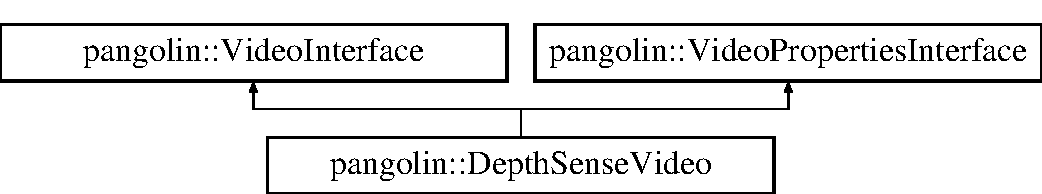
\includegraphics[height=2.000000cm]{classpangolin_1_1_depth_sense_video}
\end{center}
\end{figure}
\subsection*{Classes}
\begin{DoxyCompactItemize}
\item 
struct \hyperlink{structpangolin_1_1_depth_sense_video_1_1_sensor_config}{Sensor\+Config}
\end{DoxyCompactItemize}
\subsection*{Public Member Functions}
\begin{DoxyCompactItemize}
\item 
{\bfseries Depth\+Sense\+Video} (Depth\+Sense\+::\+Device device, Depth\+Sense\+Sensor\+Type s1, Depth\+Sense\+Sensor\+Type s2, \hyperlink{structpangolin_1_1_image_dim}{Image\+Dim} dim1, \hyperlink{structpangolin_1_1_image_dim}{Image\+Dim} dim2, unsigned int fps1, unsigned int fps2, const \hyperlink{classpangolin_1_1_uri}{Uri} \&uri)\hypertarget{classpangolin_1_1_depth_sense_video_a792a4261ff251550b93f6ed4d06642a3}{}\label{classpangolin_1_1_depth_sense_video_a792a4261ff251550b93f6ed4d06642a3}

\item 
void \hyperlink{classpangolin_1_1_depth_sense_video_a32952c0c71c897c25370843415853c7c}{Start} ()\hypertarget{classpangolin_1_1_depth_sense_video_a32952c0c71c897c25370843415853c7c}{}\label{classpangolin_1_1_depth_sense_video_a32952c0c71c897c25370843415853c7c}

\begin{DoxyCompactList}\small\item\em Implement \hyperlink{structpangolin_1_1_video_input_a74a2e3e1b87c7cbf9de9bcb39e1df128}{Video\+Input\+::\+Start()} \end{DoxyCompactList}\item 
void \hyperlink{classpangolin_1_1_depth_sense_video_aa5cc804ef512e4c22cccb856c85d5b26}{Stop} ()\hypertarget{classpangolin_1_1_depth_sense_video_aa5cc804ef512e4c22cccb856c85d5b26}{}\label{classpangolin_1_1_depth_sense_video_aa5cc804ef512e4c22cccb856c85d5b26}

\begin{DoxyCompactList}\small\item\em Implement \hyperlink{structpangolin_1_1_video_input_a8945f80194cc7ec9594db7f27e7d09b8}{Video\+Input\+::\+Stop()} \end{DoxyCompactList}\item 
size\+\_\+t \hyperlink{classpangolin_1_1_depth_sense_video_acdb3864c713fe0c6ba69b70a2f0bd770}{Size\+Bytes} () const \hypertarget{classpangolin_1_1_depth_sense_video_acdb3864c713fe0c6ba69b70a2f0bd770}{}\label{classpangolin_1_1_depth_sense_video_acdb3864c713fe0c6ba69b70a2f0bd770}

\begin{DoxyCompactList}\small\item\em Implement \hyperlink{structpangolin_1_1_video_input_a93cee5c33386973a2a51165e6bdcf40b}{Video\+Input\+::\+Size\+Bytes()} \end{DoxyCompactList}\item 
const std\+::vector$<$ \hyperlink{classpangolin_1_1_stream_info}{Stream\+Info} $>$ \& \hyperlink{classpangolin_1_1_depth_sense_video_a6a404f7d4cff4ce2a47f9140b2f2d080}{Streams} () const \hypertarget{classpangolin_1_1_depth_sense_video_a6a404f7d4cff4ce2a47f9140b2f2d080}{}\label{classpangolin_1_1_depth_sense_video_a6a404f7d4cff4ce2a47f9140b2f2d080}

\begin{DoxyCompactList}\small\item\em Implement \hyperlink{structpangolin_1_1_video_input_a9030d775d699c39ab7b7ba378c007c6a}{Video\+Input\+::\+Streams()} \end{DoxyCompactList}\item 
bool \hyperlink{classpangolin_1_1_depth_sense_video_a25a5e67d87443a9268e5845e72d29092}{Grab\+Next} (unsigned char $\ast$image, bool wait=true)\hypertarget{classpangolin_1_1_depth_sense_video_a25a5e67d87443a9268e5845e72d29092}{}\label{classpangolin_1_1_depth_sense_video_a25a5e67d87443a9268e5845e72d29092}

\begin{DoxyCompactList}\small\item\em Implement \hyperlink{structpangolin_1_1_video_input_ad3d8ff59c1ec4139320097e6e1111f32}{Video\+Input\+::\+Grab\+Next()} \end{DoxyCompactList}\item 
bool \hyperlink{classpangolin_1_1_depth_sense_video_a2ac3ea9e39741d607ed0792e23f83ede}{Grab\+Newest} (unsigned char $\ast$image, bool wait=true)\hypertarget{classpangolin_1_1_depth_sense_video_a2ac3ea9e39741d607ed0792e23f83ede}{}\label{classpangolin_1_1_depth_sense_video_a2ac3ea9e39741d607ed0792e23f83ede}

\begin{DoxyCompactList}\small\item\em Implement \hyperlink{structpangolin_1_1_video_input_a4c8ac38e3c6a3f591663aeebf645e4c6}{Video\+Input\+::\+Grab\+Newest()} \end{DoxyCompactList}\item 
const \hyperlink{classpangolin_1_1json_1_1value}{json\+::value} \& \hyperlink{classpangolin_1_1_depth_sense_video_a5c36ad7603c146e83546d203c685885b}{Device\+Properties} () const \hypertarget{classpangolin_1_1_depth_sense_video_a5c36ad7603c146e83546d203c685885b}{}\label{classpangolin_1_1_depth_sense_video_a5c36ad7603c146e83546d203c685885b}

\begin{DoxyCompactList}\small\item\em Implement Video\+Input\+::\+Device\+Properties() \end{DoxyCompactList}\item 
const \hyperlink{classpangolin_1_1json_1_1value}{json\+::value} \& \hyperlink{classpangolin_1_1_depth_sense_video_a474615f56505bf0fb635eb95dc8dbc3e}{Frame\+Properties} () const \hypertarget{classpangolin_1_1_depth_sense_video_a474615f56505bf0fb635eb95dc8dbc3e}{}\label{classpangolin_1_1_depth_sense_video_a474615f56505bf0fb635eb95dc8dbc3e}

\begin{DoxyCompactList}\small\item\em Implement Video\+Input\+::\+Device\+Properties() \end{DoxyCompactList}\end{DoxyCompactItemize}
\subsection*{Protected Member Functions}
\begin{DoxyCompactItemize}
\item 
void {\bfseries on\+New\+Color\+Sample} (Depth\+Sense\+::\+Color\+Node node, Depth\+Sense\+::\+Color\+Node\+::\+New\+Sample\+Received\+Data data)\hypertarget{classpangolin_1_1_depth_sense_video_a24bfe1ab3939214135add4274541ea79}{}\label{classpangolin_1_1_depth_sense_video_a24bfe1ab3939214135add4274541ea79}

\item 
void {\bfseries on\+New\+Depth\+Sample} (Depth\+Sense\+::\+Depth\+Node node, Depth\+Sense\+::\+Depth\+Node\+::\+New\+Sample\+Received\+Data data)\hypertarget{classpangolin_1_1_depth_sense_video_ac37f0399edc6d0610f1726dbcbda48c5}{}\label{classpangolin_1_1_depth_sense_video_ac37f0399edc6d0610f1726dbcbda48c5}

\item 
void {\bfseries Update\+Parameters} (const Depth\+Sense\+::\+Node \&node, const \hyperlink{classpangolin_1_1_uri}{Uri} \&uri)\hypertarget{classpangolin_1_1_depth_sense_video_a107e0f5e9fb28d5c1b178b39c2aeb0fb}{}\label{classpangolin_1_1_depth_sense_video_a107e0f5e9fb28d5c1b178b39c2aeb0fb}

\item 
void {\bfseries Configure\+Nodes} (const \hyperlink{classpangolin_1_1_uri}{Uri} \&uri)\hypertarget{classpangolin_1_1_depth_sense_video_a1670e4ccc178a7fe55093c3bd9f9aee6}{}\label{classpangolin_1_1_depth_sense_video_a1670e4ccc178a7fe55093c3bd9f9aee6}

\item 
void {\bfseries Configure\+Depth\+Node} (const \hyperlink{structpangolin_1_1_depth_sense_video_1_1_sensor_config}{Sensor\+Config} \&sensor\+Config, const \hyperlink{classpangolin_1_1_uri}{Uri} \&uri)\hypertarget{classpangolin_1_1_depth_sense_video_add62506c40b128168e1089c5ecf8a85f}{}\label{classpangolin_1_1_depth_sense_video_add62506c40b128168e1089c5ecf8a85f}

\item 
void {\bfseries Configure\+Color\+Node} (const \hyperlink{structpangolin_1_1_depth_sense_video_1_1_sensor_config}{Sensor\+Config} \&sensor\+Config, const \hyperlink{classpangolin_1_1_uri}{Uri} \&uri)\hypertarget{classpangolin_1_1_depth_sense_video_a4dd87d108c5fa2d40e6965d0a65d1dd1}{}\label{classpangolin_1_1_depth_sense_video_a4dd87d108c5fa2d40e6965d0a65d1dd1}

\item 
double {\bfseries Get\+Delta\+Time} () const \hypertarget{classpangolin_1_1_depth_sense_video_ad260582fdb507186d2275d21819ebfba}{}\label{classpangolin_1_1_depth_sense_video_ad260582fdb507186d2275d21819ebfba}

\end{DoxyCompactItemize}
\subsection*{Protected Attributes}
\begin{DoxyCompactItemize}
\item 
std\+::vector$<$ \hyperlink{classpangolin_1_1_stream_info}{Stream\+Info} $>$ {\bfseries streams}\hypertarget{classpangolin_1_1_depth_sense_video_a97820c8872cfbfda2343ebd38094aae7}{}\label{classpangolin_1_1_depth_sense_video_a97820c8872cfbfda2343ebd38094aae7}

\item 
\hyperlink{classpangolin_1_1json_1_1value}{json\+::value} {\bfseries device\+\_\+properties}\hypertarget{classpangolin_1_1_depth_sense_video_abd1a60dbe45641f6623f659c780e88ef}{}\label{classpangolin_1_1_depth_sense_video_abd1a60dbe45641f6623f659c780e88ef}

\item 
\hyperlink{classpangolin_1_1json_1_1value}{json\+::value} {\bfseries frame\+\_\+properties}\hypertarget{classpangolin_1_1_depth_sense_video_ae1cdcc1197e0e39b00df9dd701c31f9e}{}\label{classpangolin_1_1_depth_sense_video_ae1cdcc1197e0e39b00df9dd701c31f9e}

\item 
\hyperlink{classpangolin_1_1json_1_1value}{json\+::value} $\ast$ {\bfseries streams\+\_\+properties}\hypertarget{classpangolin_1_1_depth_sense_video_ac098237a849c756f70584911bbb0dc30}{}\label{classpangolin_1_1_depth_sense_video_ac098237a849c756f70584911bbb0dc30}

\item 
Depth\+Sense\+::\+Device {\bfseries device}\hypertarget{classpangolin_1_1_depth_sense_video_a627c580484042cf8aedafd2f5e057bc2}{}\label{classpangolin_1_1_depth_sense_video_a627c580484042cf8aedafd2f5e057bc2}

\item 
Depth\+Sense\+::\+Depth\+Node {\bfseries g\+\_\+dnode}\hypertarget{classpangolin_1_1_depth_sense_video_a3c62b82b532e8663159c2a88e6e94e05}{}\label{classpangolin_1_1_depth_sense_video_a3c62b82b532e8663159c2a88e6e94e05}

\item 
Depth\+Sense\+::\+Color\+Node {\bfseries g\+\_\+cnode}\hypertarget{classpangolin_1_1_depth_sense_video_a062dfae8a4d256ea32507ffa8bf54f74}{}\label{classpangolin_1_1_depth_sense_video_a062dfae8a4d256ea32507ffa8bf54f74}

\item 
unsigned char $\ast$ {\bfseries fill\+\_\+image}\hypertarget{classpangolin_1_1_depth_sense_video_a2c17c2fefded23925e7c64b188164c4a}{}\label{classpangolin_1_1_depth_sense_video_a2c17c2fefded23925e7c64b188164c4a}

\item 
int {\bfseries depthmap\+\_\+stream}\hypertarget{classpangolin_1_1_depth_sense_video_a6dda8481d4185db9e5ed7e7044409b5d}{}\label{classpangolin_1_1_depth_sense_video_a6dda8481d4185db9e5ed7e7044409b5d}

\item 
int {\bfseries rgb\+\_\+stream}\hypertarget{classpangolin_1_1_depth_sense_video_a1f58c99716587aa8ecc4f442778fdc4c}{}\label{classpangolin_1_1_depth_sense_video_a1f58c99716587aa8ecc4f442778fdc4c}

\item 
int {\bfseries got\+Depth}\hypertarget{classpangolin_1_1_depth_sense_video_a5bd47c119eff7792768487b54c4bff01}{}\label{classpangolin_1_1_depth_sense_video_a5bd47c119eff7792768487b54c4bff01}

\item 
int {\bfseries got\+Color}\hypertarget{classpangolin_1_1_depth_sense_video_a1d6bca7d57bdaab9955dec36b6d120d9}{}\label{classpangolin_1_1_depth_sense_video_a1d6bca7d57bdaab9955dec36b6d120d9}

\item 
boostd\+::mutex {\bfseries update\+\_\+mutex}\hypertarget{classpangolin_1_1_depth_sense_video_a928f9cc22afb1cb78b58e716e8c8d7c6}{}\label{classpangolin_1_1_depth_sense_video_a928f9cc22afb1cb78b58e716e8c8d7c6}

\item 
boostd\+::condition\+\_\+variable {\bfseries cond\+\_\+image\+\_\+filled}\hypertarget{classpangolin_1_1_depth_sense_video_af0c2dfb8f8a6dd9035e66b4a36b2cf54}{}\label{classpangolin_1_1_depth_sense_video_af0c2dfb8f8a6dd9035e66b4a36b2cf54}

\item 
boostd\+::condition\+\_\+variable {\bfseries cond\+\_\+image\+\_\+requested}\hypertarget{classpangolin_1_1_depth_sense_video_a6d004f68191ff42f6619bca73b37c05f}{}\label{classpangolin_1_1_depth_sense_video_a6d004f68191ff42f6619bca73b37c05f}

\item 
\hyperlink{structpangolin_1_1_depth_sense_video_1_1_sensor_config}{Sensor\+Config} {\bfseries sensor\+Config} \mbox{[}2\mbox{]}\hypertarget{classpangolin_1_1_depth_sense_video_a9c01629371bfec1ed8282fabac2f0fee}{}\label{classpangolin_1_1_depth_sense_video_a9c01629371bfec1ed8282fabac2f0fee}

\item 
bool {\bfseries enable\+Depth}\hypertarget{classpangolin_1_1_depth_sense_video_a8bd09cc5c54d7305fbc136e4e299101e}{}\label{classpangolin_1_1_depth_sense_video_a8bd09cc5c54d7305fbc136e4e299101e}

\item 
bool {\bfseries enable\+Color}\hypertarget{classpangolin_1_1_depth_sense_video_a63be548747807cd64b465cd38053342c}{}\label{classpangolin_1_1_depth_sense_video_a63be548747807cd64b465cd38053342c}

\item 
double {\bfseries depth\+Ts}\hypertarget{classpangolin_1_1_depth_sense_video_ab81444a7895bcfd83ea42968f9b81387}{}\label{classpangolin_1_1_depth_sense_video_ab81444a7895bcfd83ea42968f9b81387}

\item 
double {\bfseries color\+Ts}\hypertarget{classpangolin_1_1_depth_sense_video_abcd55c1cba7c4172811b3eac378b00ab}{}\label{classpangolin_1_1_depth_sense_video_abcd55c1cba7c4172811b3eac378b00ab}

\item 
size\+\_\+t {\bfseries size\+\_\+bytes}\hypertarget{classpangolin_1_1_depth_sense_video_a67fb6c0cfa3323df304e85911c735168}{}\label{classpangolin_1_1_depth_sense_video_a67fb6c0cfa3323df304e85911c735168}

\end{DoxyCompactItemize}


The documentation for this class was generated from the following file\+:\begin{DoxyCompactItemize}
\item 
/home/gapo/meng/deps/pangolin/include/pangolin/video/drivers/depthsense.\+h\end{DoxyCompactItemize}

\hypertarget{structpangolin_1_1_dimension_stats}{}\section{pangolin\+:\+:Dimension\+Stats Struct Reference}
\label{structpangolin_1_1_dimension_stats}\index{pangolin\+::\+Dimension\+Stats@{pangolin\+::\+Dimension\+Stats}}


Simple statistics recorded for a logged input dimension.  




{\ttfamily \#include $<$datalog.\+h$>$}

\subsection*{Public Attributes}
\begin{DoxyCompactItemize}
\item 
bool {\bfseries is\+Monotonic}\hypertarget{structpangolin_1_1_dimension_stats_a519a9658616664fc612d5046c642b2cd}{}\label{structpangolin_1_1_dimension_stats_a519a9658616664fc612d5046c642b2cd}

\item 
float {\bfseries sum}\hypertarget{structpangolin_1_1_dimension_stats_abf62d532ffe75850ddca3ab008d18534}{}\label{structpangolin_1_1_dimension_stats_abf62d532ffe75850ddca3ab008d18534}

\item 
float {\bfseries sum\+\_\+sq}\hypertarget{structpangolin_1_1_dimension_stats_a5ab51d111dffde00e24321da1ef9da27}{}\label{structpangolin_1_1_dimension_stats_a5ab51d111dffde00e24321da1ef9da27}

\item 
float {\bfseries min}\hypertarget{structpangolin_1_1_dimension_stats_a3637f70ef331232b4fabbef2b23e0841}{}\label{structpangolin_1_1_dimension_stats_a3637f70ef331232b4fabbef2b23e0841}

\item 
float {\bfseries max}\hypertarget{structpangolin_1_1_dimension_stats_af9b6b88f17e28c19ee21359009380251}{}\label{structpangolin_1_1_dimension_stats_af9b6b88f17e28c19ee21359009380251}

\end{DoxyCompactItemize}


\subsection{Detailed Description}
Simple statistics recorded for a logged input dimension. 

The documentation for this struct was generated from the following file\+:\begin{DoxyCompactItemize}
\item 
/home/gapo/meng/deps/pangolin/include/pangolin/plot/datalog.\+h\end{DoxyCompactItemize}

\hypertarget{structpangolin_1_1json_1_1null__parse__context_1_1dummy__str}{}\section{pangolin\+:\+:json\+:\+:null\+\_\+parse\+\_\+context\+:\+:dummy\+\_\+str Struct Reference}
\label{structpangolin_1_1json_1_1null__parse__context_1_1dummy__str}\index{pangolin\+::json\+::null\+\_\+parse\+\_\+context\+::dummy\+\_\+str@{pangolin\+::json\+::null\+\_\+parse\+\_\+context\+::dummy\+\_\+str}}
\subsection*{Public Member Functions}
\begin{DoxyCompactItemize}
\item 
void {\bfseries push\+\_\+back} (int)\hypertarget{structpangolin_1_1json_1_1null__parse__context_1_1dummy__str_a699530fb46d1c188e5e5ced1020b6607}{}\label{structpangolin_1_1json_1_1null__parse__context_1_1dummy__str_a699530fb46d1c188e5e5ced1020b6607}

\end{DoxyCompactItemize}


The documentation for this struct was generated from the following file\+:\begin{DoxyCompactItemize}
\item 
/home/gapo/meng/deps/pangolin/include/pangolin/utils/picojson.\+h\end{DoxyCompactItemize}

\hypertarget{structpangolin_1_1enable__if}{}\section{pangolin\+:\+:enable\+\_\+if$<$ Cond, T $>$ Struct Template Reference}
\label{structpangolin_1_1enable__if}\index{pangolin\+::enable\+\_\+if$<$ Cond, T $>$@{pangolin\+::enable\+\_\+if$<$ Cond, T $>$}}
Inheritance diagram for pangolin\+:\+:enable\+\_\+if$<$ Cond, T $>$\+:\begin{figure}[H]
\begin{center}
\leavevmode
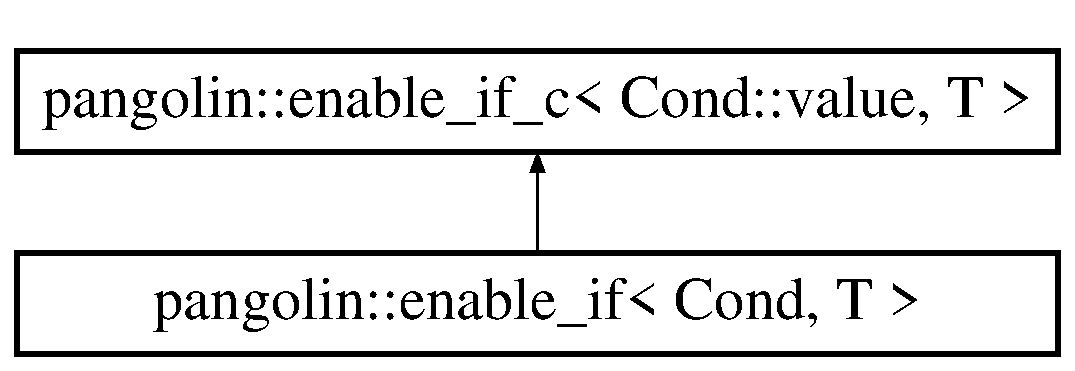
\includegraphics[height=2.000000cm]{structpangolin_1_1enable__if}
\end{center}
\end{figure}
\subsection*{Additional Inherited Members}


The documentation for this struct was generated from the following file\+:\begin{DoxyCompactItemize}
\item 
/home/gapo/meng/deps/pangolin/include/pangolin/compat/type\+\_\+traits.\+h\end{DoxyCompactItemize}

\hypertarget{structpangolin_1_1enable__if__c}{}\section{pangolin\+:\+:enable\+\_\+if\+\_\+c$<$ B, T $>$ Struct Template Reference}
\label{structpangolin_1_1enable__if__c}\index{pangolin\+::enable\+\_\+if\+\_\+c$<$ B, T $>$@{pangolin\+::enable\+\_\+if\+\_\+c$<$ B, T $>$}}
\subsection*{Public Types}
\begin{DoxyCompactItemize}
\item 
typedef T {\bfseries type}\hypertarget{structpangolin_1_1enable__if__c_a621047603a2f69e5a5abcbf783753a48}{}\label{structpangolin_1_1enable__if__c_a621047603a2f69e5a5abcbf783753a48}

\end{DoxyCompactItemize}


The documentation for this struct was generated from the following file\+:\begin{DoxyCompactItemize}
\item 
/home/gapo/meng/deps/pangolin/include/pangolin/compat/type\+\_\+traits.\+h\end{DoxyCompactItemize}

\hypertarget{structpangolin_1_1enable__if__c_3_01false_00_01_t_01_4}{}\section{pangolin\+:\+:enable\+\_\+if\+\_\+c$<$ false, T $>$ Struct Template Reference}
\label{structpangolin_1_1enable__if__c_3_01false_00_01_t_01_4}\index{pangolin\+::enable\+\_\+if\+\_\+c$<$ false, T $>$@{pangolin\+::enable\+\_\+if\+\_\+c$<$ false, T $>$}}


The documentation for this struct was generated from the following file\+:\begin{DoxyCompactItemize}
\item 
/home/gapo/meng/deps/pangolin/include/pangolin/compat/type\+\_\+traits.\+h\end{DoxyCompactItemize}

\hypertarget{classpangolin_1_1_ffmpeg_converter}{}\section{pangolin\+:\+:Ffmpeg\+Converter Class Reference}
\label{classpangolin_1_1_ffmpeg_converter}\index{pangolin\+::\+Ffmpeg\+Converter@{pangolin\+::\+Ffmpeg\+Converter}}
Inheritance diagram for pangolin\+:\+:Ffmpeg\+Converter\+:\begin{figure}[H]
\begin{center}
\leavevmode
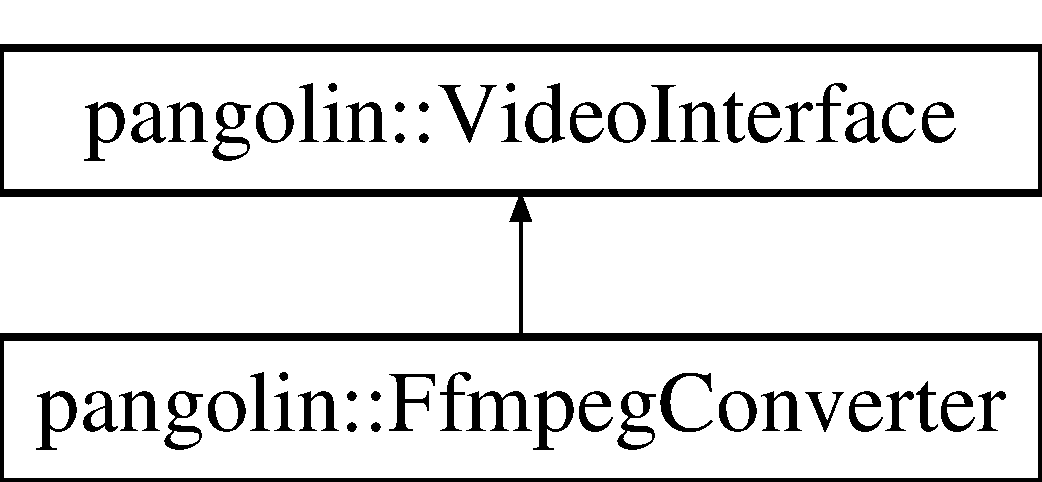
\includegraphics[height=2.000000cm]{classpangolin_1_1_ffmpeg_converter}
\end{center}
\end{figure}
\subsection*{Public Member Functions}
\begin{DoxyCompactItemize}
\item 
{\bfseries Ffmpeg\+Converter} (\hyperlink{structpangolin_1_1_video_interface}{Video\+Interface} $\ast$videoin, const std\+::string pixelfmtout=\char`\"{}R\+G\+B24\char`\"{}, Ffmpeg\+Method method=F\+F\+M\+P\+E\+G\+\_\+\+P\+O\+I\+NT)\hypertarget{classpangolin_1_1_ffmpeg_converter_a69b5561ab5a5a8e8cab92f1ecdd13212}{}\label{classpangolin_1_1_ffmpeg_converter_a69b5561ab5a5a8e8cab92f1ecdd13212}

\item 
void \hyperlink{classpangolin_1_1_ffmpeg_converter_a25e3030bf21b559196b14c27aa1e53e3}{Start} ()\hypertarget{classpangolin_1_1_ffmpeg_converter_a25e3030bf21b559196b14c27aa1e53e3}{}\label{classpangolin_1_1_ffmpeg_converter_a25e3030bf21b559196b14c27aa1e53e3}

\begin{DoxyCompactList}\small\item\em Implement \hyperlink{structpangolin_1_1_video_input_a74a2e3e1b87c7cbf9de9bcb39e1df128}{Video\+Input\+::\+Start()} \end{DoxyCompactList}\item 
void \hyperlink{classpangolin_1_1_ffmpeg_converter_a8e3a0216a517525c104bfc753050a463}{Stop} ()\hypertarget{classpangolin_1_1_ffmpeg_converter_a8e3a0216a517525c104bfc753050a463}{}\label{classpangolin_1_1_ffmpeg_converter_a8e3a0216a517525c104bfc753050a463}

\begin{DoxyCompactList}\small\item\em Implement \hyperlink{structpangolin_1_1_video_input_a8945f80194cc7ec9594db7f27e7d09b8}{Video\+Input\+::\+Stop()} \end{DoxyCompactList}\item 
size\+\_\+t \hyperlink{classpangolin_1_1_ffmpeg_converter_a6f251afa8078734cf1d8ee334746c8f7}{Size\+Bytes} () const \hypertarget{classpangolin_1_1_ffmpeg_converter_a6f251afa8078734cf1d8ee334746c8f7}{}\label{classpangolin_1_1_ffmpeg_converter_a6f251afa8078734cf1d8ee334746c8f7}

\begin{DoxyCompactList}\small\item\em Implement \hyperlink{structpangolin_1_1_video_input_a93cee5c33386973a2a51165e6bdcf40b}{Video\+Input\+::\+Size\+Bytes()} \end{DoxyCompactList}\item 
const std\+::vector$<$ \hyperlink{classpangolin_1_1_stream_info}{Stream\+Info} $>$ \& \hyperlink{classpangolin_1_1_ffmpeg_converter_a52ba3ad0dac71cba146b87257c8d546c}{Streams} () const \hypertarget{classpangolin_1_1_ffmpeg_converter_a52ba3ad0dac71cba146b87257c8d546c}{}\label{classpangolin_1_1_ffmpeg_converter_a52ba3ad0dac71cba146b87257c8d546c}

\begin{DoxyCompactList}\small\item\em Implement \hyperlink{structpangolin_1_1_video_input_a9030d775d699c39ab7b7ba378c007c6a}{Video\+Input\+::\+Streams()} \end{DoxyCompactList}\item 
bool \hyperlink{classpangolin_1_1_ffmpeg_converter_a967ca60f307208300a216b044938375f}{Grab\+Next} (unsigned char $\ast$image, bool wait=true)\hypertarget{classpangolin_1_1_ffmpeg_converter_a967ca60f307208300a216b044938375f}{}\label{classpangolin_1_1_ffmpeg_converter_a967ca60f307208300a216b044938375f}

\begin{DoxyCompactList}\small\item\em Implement \hyperlink{structpangolin_1_1_video_input_ad3d8ff59c1ec4139320097e6e1111f32}{Video\+Input\+::\+Grab\+Next()} \end{DoxyCompactList}\item 
bool \hyperlink{classpangolin_1_1_ffmpeg_converter_a86127ecc83c86d6e31685c2779eea482}{Grab\+Newest} (unsigned char $\ast$image, bool wait=true)\hypertarget{classpangolin_1_1_ffmpeg_converter_a86127ecc83c86d6e31685c2779eea482}{}\label{classpangolin_1_1_ffmpeg_converter_a86127ecc83c86d6e31685c2779eea482}

\begin{DoxyCompactList}\small\item\em Implement \hyperlink{structpangolin_1_1_video_input_a4c8ac38e3c6a3f591663aeebf645e4c6}{Video\+Input\+::\+Grab\+Newest()} \end{DoxyCompactList}\end{DoxyCompactItemize}
\subsection*{Protected Attributes}
\begin{DoxyCompactItemize}
\item 
std\+::vector$<$ \hyperlink{classpangolin_1_1_stream_info}{Stream\+Info} $>$ {\bfseries streams}\hypertarget{classpangolin_1_1_ffmpeg_converter_a2b1efbd33002a11a0eacf1ba2c43571c}{}\label{classpangolin_1_1_ffmpeg_converter_a2b1efbd33002a11a0eacf1ba2c43571c}

\item 
\hyperlink{structpangolin_1_1_video_interface}{Video\+Interface} $\ast$ {\bfseries videoin}\hypertarget{classpangolin_1_1_ffmpeg_converter_ae7f5f68d7a45fd0ce4e1d5d476099a26}{}\label{classpangolin_1_1_ffmpeg_converter_ae7f5f68d7a45fd0ce4e1d5d476099a26}

\item 
Sws\+Context $\ast$ {\bfseries img\+\_\+convert\+\_\+ctx}\hypertarget{classpangolin_1_1_ffmpeg_converter_aea617eee3da7ec80b89111fa169fa35e}{}\label{classpangolin_1_1_ffmpeg_converter_aea617eee3da7ec80b89111fa169fa35e}

\item 
Pixel\+Format {\bfseries fmtsrc}\hypertarget{classpangolin_1_1_ffmpeg_converter_a473f55dc1219d571b121c70f77780c7c}{}\label{classpangolin_1_1_ffmpeg_converter_a473f55dc1219d571b121c70f77780c7c}

\item 
Pixel\+Format {\bfseries fmtdst}\hypertarget{classpangolin_1_1_ffmpeg_converter_a22f1af94ed4f48c49128f0264e28ff1b}{}\label{classpangolin_1_1_ffmpeg_converter_a22f1af94ed4f48c49128f0264e28ff1b}

\item 
A\+V\+Frame $\ast$ {\bfseries avsrc}\hypertarget{classpangolin_1_1_ffmpeg_converter_accf06173a714645a808be178f8d76e98}{}\label{classpangolin_1_1_ffmpeg_converter_accf06173a714645a808be178f8d76e98}

\item 
A\+V\+Frame $\ast$ {\bfseries avdst}\hypertarget{classpangolin_1_1_ffmpeg_converter_ac630a10c0376d0a12bec9df520d5ac62}{}\label{classpangolin_1_1_ffmpeg_converter_ac630a10c0376d0a12bec9df520d5ac62}

\item 
uint8\+\_\+t $\ast$ {\bfseries bufsrc}\hypertarget{classpangolin_1_1_ffmpeg_converter_aca2fa5e0c62c88a20db742c9f1ae6496}{}\label{classpangolin_1_1_ffmpeg_converter_aca2fa5e0c62c88a20db742c9f1ae6496}

\item 
uint8\+\_\+t $\ast$ {\bfseries bufdst}\hypertarget{classpangolin_1_1_ffmpeg_converter_aaad093a9400770306758419b14617d3f}{}\label{classpangolin_1_1_ffmpeg_converter_aaad093a9400770306758419b14617d3f}

\item 
int {\bfseries numbytessrc}\hypertarget{classpangolin_1_1_ffmpeg_converter_a29d46022dbf371499178da6a2790b584}{}\label{classpangolin_1_1_ffmpeg_converter_a29d46022dbf371499178da6a2790b584}

\item 
int {\bfseries numbytesdst}\hypertarget{classpangolin_1_1_ffmpeg_converter_a137ced15d2543031b8b6a643641a7ab0}{}\label{classpangolin_1_1_ffmpeg_converter_a137ced15d2543031b8b6a643641a7ab0}

\item 
unsigned {\bfseries w}\hypertarget{classpangolin_1_1_ffmpeg_converter_ae9e979fcd4f74680da019cb2ecfebb0e}{}\label{classpangolin_1_1_ffmpeg_converter_ae9e979fcd4f74680da019cb2ecfebb0e}

\item 
unsigned {\bfseries h}\hypertarget{classpangolin_1_1_ffmpeg_converter_aa0e124d177b5b4a3d7fb69ca9de2e98f}{}\label{classpangolin_1_1_ffmpeg_converter_aa0e124d177b5b4a3d7fb69ca9de2e98f}

\end{DoxyCompactItemize}


The documentation for this class was generated from the following file\+:\begin{DoxyCompactItemize}
\item 
/home/gapo/meng/deps/pangolin/include/pangolin/video/drivers/ffmpeg.\+h\end{DoxyCompactItemize}

\hypertarget{classpangolin_1_1_ffmpeg_video}{}\section{pangolin\+:\+:Ffmpeg\+Video Class Reference}
\label{classpangolin_1_1_ffmpeg_video}\index{pangolin\+::\+Ffmpeg\+Video@{pangolin\+::\+Ffmpeg\+Video}}
Inheritance diagram for pangolin\+:\+:Ffmpeg\+Video\+:\begin{figure}[H]
\begin{center}
\leavevmode
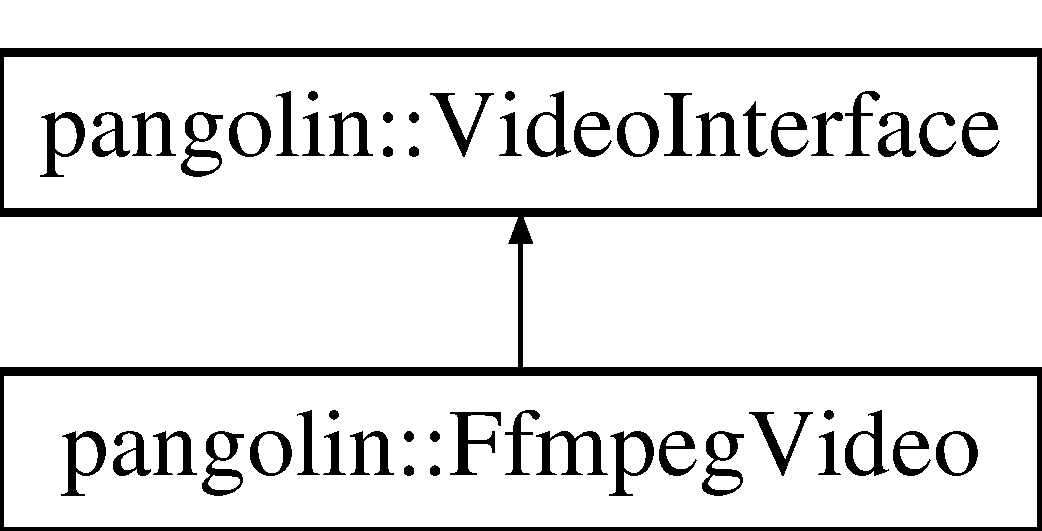
\includegraphics[height=2.000000cm]{classpangolin_1_1_ffmpeg_video}
\end{center}
\end{figure}
\subsection*{Public Member Functions}
\begin{DoxyCompactItemize}
\item 
{\bfseries Ffmpeg\+Video} (const std\+::string filename, const std\+::string fmtout=\char`\"{}R\+G\+B24\char`\"{}, const std\+::string codec\+\_\+hint=\char`\"{}\char`\"{}, bool dump\+\_\+info=false, int user\+\_\+video\+\_\+stream=-\/1)\hypertarget{classpangolin_1_1_ffmpeg_video_a0aaac4d5d20e0aa4cdf9e057424039dc}{}\label{classpangolin_1_1_ffmpeg_video_a0aaac4d5d20e0aa4cdf9e057424039dc}

\item 
void \hyperlink{classpangolin_1_1_ffmpeg_video_a918cd0530ef8e92a11cc1568082dbe6f}{Start} ()\hypertarget{classpangolin_1_1_ffmpeg_video_a918cd0530ef8e92a11cc1568082dbe6f}{}\label{classpangolin_1_1_ffmpeg_video_a918cd0530ef8e92a11cc1568082dbe6f}

\begin{DoxyCompactList}\small\item\em Implement \hyperlink{structpangolin_1_1_video_input_a74a2e3e1b87c7cbf9de9bcb39e1df128}{Video\+Input\+::\+Start()} \end{DoxyCompactList}\item 
void \hyperlink{classpangolin_1_1_ffmpeg_video_a5da92c12324d7a9f04c76366b13b361e}{Stop} ()\hypertarget{classpangolin_1_1_ffmpeg_video_a5da92c12324d7a9f04c76366b13b361e}{}\label{classpangolin_1_1_ffmpeg_video_a5da92c12324d7a9f04c76366b13b361e}

\begin{DoxyCompactList}\small\item\em Implement \hyperlink{structpangolin_1_1_video_input_a8945f80194cc7ec9594db7f27e7d09b8}{Video\+Input\+::\+Stop()} \end{DoxyCompactList}\item 
size\+\_\+t \hyperlink{classpangolin_1_1_ffmpeg_video_ab45d5acd24526f05004815722fdcd645}{Size\+Bytes} () const \hypertarget{classpangolin_1_1_ffmpeg_video_ab45d5acd24526f05004815722fdcd645}{}\label{classpangolin_1_1_ffmpeg_video_ab45d5acd24526f05004815722fdcd645}

\begin{DoxyCompactList}\small\item\em Implement \hyperlink{structpangolin_1_1_video_input_a93cee5c33386973a2a51165e6bdcf40b}{Video\+Input\+::\+Size\+Bytes()} \end{DoxyCompactList}\item 
const std\+::vector$<$ \hyperlink{classpangolin_1_1_stream_info}{Stream\+Info} $>$ \& \hyperlink{classpangolin_1_1_ffmpeg_video_a510314ebff17c36606cf7d1f65c98934}{Streams} () const \hypertarget{classpangolin_1_1_ffmpeg_video_a510314ebff17c36606cf7d1f65c98934}{}\label{classpangolin_1_1_ffmpeg_video_a510314ebff17c36606cf7d1f65c98934}

\begin{DoxyCompactList}\small\item\em Implement \hyperlink{structpangolin_1_1_video_input_a9030d775d699c39ab7b7ba378c007c6a}{Video\+Input\+::\+Streams()} \end{DoxyCompactList}\item 
bool \hyperlink{classpangolin_1_1_ffmpeg_video_a724f49203ba3d5053edea3a00c227d44}{Grab\+Next} (unsigned char $\ast$image, bool wait=true)\hypertarget{classpangolin_1_1_ffmpeg_video_a724f49203ba3d5053edea3a00c227d44}{}\label{classpangolin_1_1_ffmpeg_video_a724f49203ba3d5053edea3a00c227d44}

\begin{DoxyCompactList}\small\item\em Implement \hyperlink{structpangolin_1_1_video_input_ad3d8ff59c1ec4139320097e6e1111f32}{Video\+Input\+::\+Grab\+Next()} \end{DoxyCompactList}\item 
bool \hyperlink{classpangolin_1_1_ffmpeg_video_ac1c3386eaaee6d3f8de590a635b59106}{Grab\+Newest} (unsigned char $\ast$image, bool wait=true)\hypertarget{classpangolin_1_1_ffmpeg_video_ac1c3386eaaee6d3f8de590a635b59106}{}\label{classpangolin_1_1_ffmpeg_video_ac1c3386eaaee6d3f8de590a635b59106}

\begin{DoxyCompactList}\small\item\em Implement \hyperlink{structpangolin_1_1_video_input_a4c8ac38e3c6a3f591663aeebf645e4c6}{Video\+Input\+::\+Grab\+Newest()} \end{DoxyCompactList}\end{DoxyCompactItemize}
\subsection*{Protected Member Functions}
\begin{DoxyCompactItemize}
\item 
void {\bfseries Init\+Url} (const std\+::string filename, const std\+::string fmtout=\char`\"{}R\+G\+B24\char`\"{}, const std\+::string codec\+\_\+hint=\char`\"{}\char`\"{}, bool dump\+\_\+info=false, int user\+\_\+video\+\_\+stream=-\/1)\hypertarget{classpangolin_1_1_ffmpeg_video_a29ea654733c7355d36e4f4ba246dd3be}{}\label{classpangolin_1_1_ffmpeg_video_a29ea654733c7355d36e4f4ba246dd3be}

\end{DoxyCompactItemize}
\subsection*{Protected Attributes}
\begin{DoxyCompactItemize}
\item 
std\+::vector$<$ \hyperlink{classpangolin_1_1_stream_info}{Stream\+Info} $>$ {\bfseries streams}\hypertarget{classpangolin_1_1_ffmpeg_video_a33740101213d676377d61db21ff38a7c}{}\label{classpangolin_1_1_ffmpeg_video_a33740101213d676377d61db21ff38a7c}

\item 
Sws\+Context $\ast$ {\bfseries img\+\_\+convert\+\_\+ctx}\hypertarget{classpangolin_1_1_ffmpeg_video_a91e245cf35b771898638aa4974c097be}{}\label{classpangolin_1_1_ffmpeg_video_a91e245cf35b771898638aa4974c097be}

\item 
A\+V\+Format\+Context $\ast$ {\bfseries p\+Format\+Ctx}\hypertarget{classpangolin_1_1_ffmpeg_video_a98e9b20fec415cb89a0036ec1046e1db}{}\label{classpangolin_1_1_ffmpeg_video_a98e9b20fec415cb89a0036ec1046e1db}

\item 
int {\bfseries video\+Stream}\hypertarget{classpangolin_1_1_ffmpeg_video_a9533107dc47d7682efd3eb7d8cbe670d}{}\label{classpangolin_1_1_ffmpeg_video_a9533107dc47d7682efd3eb7d8cbe670d}

\item 
int {\bfseries audio\+Stream}\hypertarget{classpangolin_1_1_ffmpeg_video_a6151c955129b48bca1e658ab3f8c9f48}{}\label{classpangolin_1_1_ffmpeg_video_a6151c955129b48bca1e658ab3f8c9f48}

\item 
A\+V\+Codec\+Context $\ast$ {\bfseries p\+Vid\+Codec\+Ctx}\hypertarget{classpangolin_1_1_ffmpeg_video_a848bc22224fa78db1c10f7e9f6d9a5a5}{}\label{classpangolin_1_1_ffmpeg_video_a848bc22224fa78db1c10f7e9f6d9a5a5}

\item 
A\+V\+Codec\+Context $\ast$ {\bfseries p\+Aud\+Codec\+Ctx}\hypertarget{classpangolin_1_1_ffmpeg_video_a4d6108e0c11307fce448a7ec1b829d9f}{}\label{classpangolin_1_1_ffmpeg_video_a4d6108e0c11307fce448a7ec1b829d9f}

\item 
A\+V\+Codec $\ast$ {\bfseries p\+Vid\+Codec}\hypertarget{classpangolin_1_1_ffmpeg_video_aa67b5074b353911aaca08ce2d485ab53}{}\label{classpangolin_1_1_ffmpeg_video_aa67b5074b353911aaca08ce2d485ab53}

\item 
A\+V\+Codec $\ast$ {\bfseries p\+Aud\+Codec}\hypertarget{classpangolin_1_1_ffmpeg_video_ac5e55f322a785ec3bec63f3526d2a29d}{}\label{classpangolin_1_1_ffmpeg_video_ac5e55f322a785ec3bec63f3526d2a29d}

\item 
A\+V\+Frame $\ast$ {\bfseries p\+Frame}\hypertarget{classpangolin_1_1_ffmpeg_video_afcaf4367e2165016cba0bc6d53885f67}{}\label{classpangolin_1_1_ffmpeg_video_afcaf4367e2165016cba0bc6d53885f67}

\item 
A\+V\+Frame $\ast$ {\bfseries p\+Frame\+Out}\hypertarget{classpangolin_1_1_ffmpeg_video_afd159be76fca1627679e33241c0983e4}{}\label{classpangolin_1_1_ffmpeg_video_afd159be76fca1627679e33241c0983e4}

\item 
A\+V\+Packet {\bfseries packet}\hypertarget{classpangolin_1_1_ffmpeg_video_aeea5ad8a8a8028895d4690bd68c3248f}{}\label{classpangolin_1_1_ffmpeg_video_aeea5ad8a8a8028895d4690bd68c3248f}

\item 
int {\bfseries num\+Bytes\+Out}\hypertarget{classpangolin_1_1_ffmpeg_video_a52c23d3a5bb360cf82dd4e715d5712ad}{}\label{classpangolin_1_1_ffmpeg_video_a52c23d3a5bb360cf82dd4e715d5712ad}

\item 
uint8\+\_\+t $\ast$ {\bfseries buffer}\hypertarget{classpangolin_1_1_ffmpeg_video_a2479d68835213b014cefc60158b2e77a}{}\label{classpangolin_1_1_ffmpeg_video_a2479d68835213b014cefc60158b2e77a}

\item 
Pixel\+Format {\bfseries fmtout}\hypertarget{classpangolin_1_1_ffmpeg_video_aae8ae4a5e6b6635b1da6a6e361dd5b1c}{}\label{classpangolin_1_1_ffmpeg_video_aae8ae4a5e6b6635b1da6a6e361dd5b1c}

\end{DoxyCompactItemize}


The documentation for this class was generated from the following file\+:\begin{DoxyCompactItemize}
\item 
/home/gapo/meng/deps/pangolin/include/pangolin/video/drivers/ffmpeg.\+h\end{DoxyCompactItemize}

\hypertarget{classpangolin_1_1_ffmpeg_video_output}{}\section{pangolin\+:\+:Ffmpeg\+Video\+Output Class Reference}
\label{classpangolin_1_1_ffmpeg_video_output}\index{pangolin\+::\+Ffmpeg\+Video\+Output@{pangolin\+::\+Ffmpeg\+Video\+Output}}
Inheritance diagram for pangolin\+:\+:Ffmpeg\+Video\+Output\+:\begin{figure}[H]
\begin{center}
\leavevmode
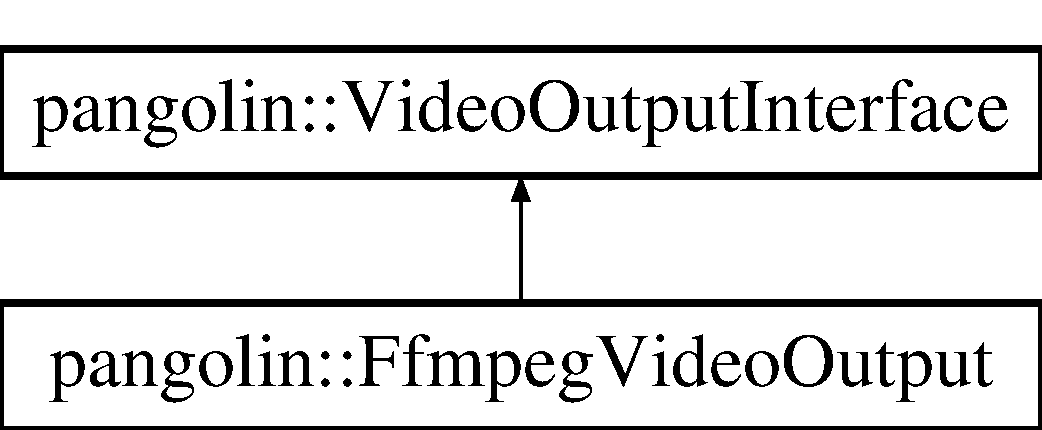
\includegraphics[height=2.000000cm]{classpangolin_1_1_ffmpeg_video_output}
\end{center}
\end{figure}
\subsection*{Public Member Functions}
\begin{DoxyCompactItemize}
\item 
{\bfseries Ffmpeg\+Video\+Output} (const std\+::string \&filename, int base\+\_\+frame\+\_\+rate, int bit\+\_\+rate)\hypertarget{classpangolin_1_1_ffmpeg_video_output_a71dac37bc51715e713c1d62603d6d4b3}{}\label{classpangolin_1_1_ffmpeg_video_output_a71dac37bc51715e713c1d62603d6d4b3}

\item 
const std\+::vector$<$ \hyperlink{classpangolin_1_1_stream_info}{Stream\+Info} $>$ \& \hyperlink{classpangolin_1_1_ffmpeg_video_output_afd0b368ca1d399254f7f46de4aad952b}{Streams} () const \hypertarget{classpangolin_1_1_ffmpeg_video_output_afd0b368ca1d399254f7f46de4aad952b}{}\label{classpangolin_1_1_ffmpeg_video_output_afd0b368ca1d399254f7f46de4aad952b}

\begin{DoxyCompactList}\small\item\em Get format and dimensions of all video streams. \end{DoxyCompactList}\item 
void {\bfseries Set\+Streams} (const std\+::vector$<$ \hyperlink{classpangolin_1_1_stream_info}{Stream\+Info} $>$ \&streams, const std\+::string \&uri, const \hyperlink{classpangolin_1_1json_1_1value}{json\+::value} \&properties)\hypertarget{classpangolin_1_1_ffmpeg_video_output_ae9f22da72c1857595684a3d5c211a080}{}\label{classpangolin_1_1_ffmpeg_video_output_ae9f22da72c1857595684a3d5c211a080}

\item 
int {\bfseries Write\+Streams} (unsigned char $\ast$data, const \hyperlink{classpangolin_1_1json_1_1value}{json\+::value} \&frame\+\_\+properties)\hypertarget{classpangolin_1_1_ffmpeg_video_output_ad78e9b60c966b2d2e39536c4a7661163}{}\label{classpangolin_1_1_ffmpeg_video_output_ad78e9b60c966b2d2e39536c4a7661163}

\end{DoxyCompactItemize}
\subsection*{Protected Member Functions}
\begin{DoxyCompactItemize}
\item 
void {\bfseries Initialise} (std\+::string filename)\hypertarget{classpangolin_1_1_ffmpeg_video_output_a48d467d91ed75ad84a9f8d34c89ac0aa}{}\label{classpangolin_1_1_ffmpeg_video_output_a48d467d91ed75ad84a9f8d34c89ac0aa}

\item 
void {\bfseries Start\+Stream} ()\hypertarget{classpangolin_1_1_ffmpeg_video_output_a99d272f5e6b7b72110a7c79c3d2b5b1a}{}\label{classpangolin_1_1_ffmpeg_video_output_a99d272f5e6b7b72110a7c79c3d2b5b1a}

\item 
void {\bfseries Close} ()\hypertarget{classpangolin_1_1_ffmpeg_video_output_af7097bb6c47222ee8c1a845df2cfccc6}{}\label{classpangolin_1_1_ffmpeg_video_output_af7097bb6c47222ee8c1a845df2cfccc6}

\end{DoxyCompactItemize}
\subsection*{Protected Attributes}
\begin{DoxyCompactItemize}
\item 
std\+::string {\bfseries filename}\hypertarget{classpangolin_1_1_ffmpeg_video_output_a9515e6e389e494ff801555197c17d076}{}\label{classpangolin_1_1_ffmpeg_video_output_a9515e6e389e494ff801555197c17d076}

\item 
bool {\bfseries started}\hypertarget{classpangolin_1_1_ffmpeg_video_output_a39c337252b41d5680db4606f802b5e70}{}\label{classpangolin_1_1_ffmpeg_video_output_a39c337252b41d5680db4606f802b5e70}

\item 
A\+V\+Format\+Context $\ast$ {\bfseries oc}\hypertarget{classpangolin_1_1_ffmpeg_video_output_a050b84fda7d97afaf6e8d1d727740e01}{}\label{classpangolin_1_1_ffmpeg_video_output_a050b84fda7d97afaf6e8d1d727740e01}

\item 
std\+::vector$<$ Ffmpeg\+Video\+Output\+Stream $\ast$ $>$ {\bfseries streams}\hypertarget{classpangolin_1_1_ffmpeg_video_output_ade3e3ba44877ff9cb9328739794a14ce}{}\label{classpangolin_1_1_ffmpeg_video_output_ade3e3ba44877ff9cb9328739794a14ce}

\item 
std\+::vector$<$ \hyperlink{classpangolin_1_1_stream_info}{Stream\+Info} $>$ {\bfseries strs}\hypertarget{classpangolin_1_1_ffmpeg_video_output_a06f84ddb6046f2658bfab821463a83af}{}\label{classpangolin_1_1_ffmpeg_video_output_a06f84ddb6046f2658bfab821463a83af}

\item 
int {\bfseries frame\+\_\+count}\hypertarget{classpangolin_1_1_ffmpeg_video_output_acda847f4bb1fab562c1b228500e73c21}{}\label{classpangolin_1_1_ffmpeg_video_output_acda847f4bb1fab562c1b228500e73c21}

\item 
int {\bfseries base\+\_\+frame\+\_\+rate}\hypertarget{classpangolin_1_1_ffmpeg_video_output_aa0d397dc329499f9c597d1caeecfcb45}{}\label{classpangolin_1_1_ffmpeg_video_output_aa0d397dc329499f9c597d1caeecfcb45}

\item 
int {\bfseries bit\+\_\+rate}\hypertarget{classpangolin_1_1_ffmpeg_video_output_aebdc068920fdeccef39d8ce2ac768d59}{}\label{classpangolin_1_1_ffmpeg_video_output_aebdc068920fdeccef39d8ce2ac768d59}

\end{DoxyCompactItemize}
\subsection*{Friends}
\begin{DoxyCompactItemize}
\item 
class {\bfseries Ffmpeg\+Video\+Output\+Stream}\hypertarget{classpangolin_1_1_ffmpeg_video_output_a1a5cda24c7a6f613553098210e328b72}{}\label{classpangolin_1_1_ffmpeg_video_output_a1a5cda24c7a6f613553098210e328b72}

\end{DoxyCompactItemize}


The documentation for this class was generated from the following file\+:\begin{DoxyCompactItemize}
\item 
/home/gapo/meng/deps/pangolin/include/pangolin/video/drivers/ffmpeg.\+h\end{DoxyCompactItemize}

\hypertarget{classpangolin_1_1_firewire_deinterlace}{}\section{pangolin\+:\+:Firewire\+Deinterlace Class Reference}
\label{classpangolin_1_1_firewire_deinterlace}\index{pangolin\+::\+Firewire\+Deinterlace@{pangolin\+::\+Firewire\+Deinterlace}}
Inheritance diagram for pangolin\+:\+:Firewire\+Deinterlace\+:\begin{figure}[H]
\begin{center}
\leavevmode
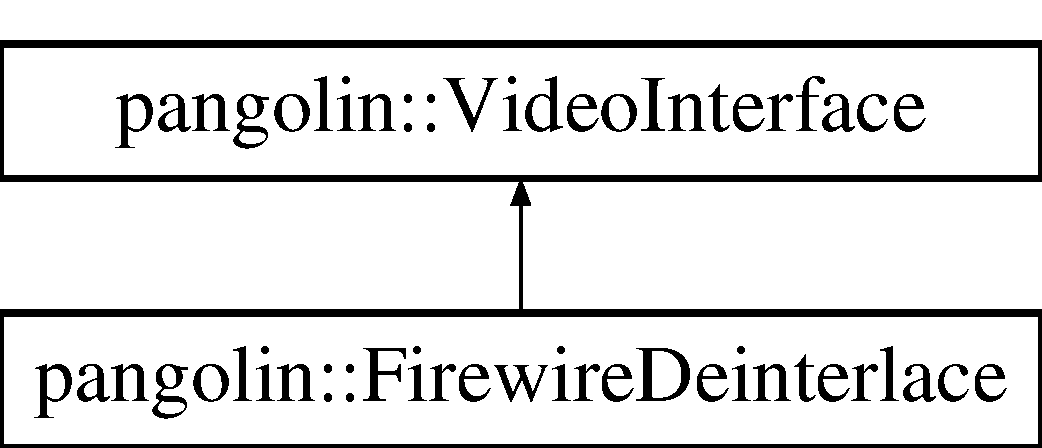
\includegraphics[height=2.000000cm]{classpangolin_1_1_firewire_deinterlace}
\end{center}
\end{figure}
\subsection*{Public Member Functions}
\begin{DoxyCompactItemize}
\item 
{\bfseries Firewire\+Deinterlace} (\hyperlink{structpangolin_1_1_video_interface}{Video\+Interface} $\ast$videoin)\hypertarget{classpangolin_1_1_firewire_deinterlace_a73c8249ab0a378c53126c1eee1cbeb31}{}\label{classpangolin_1_1_firewire_deinterlace_a73c8249ab0a378c53126c1eee1cbeb31}

\item 
size\+\_\+t \hyperlink{classpangolin_1_1_firewire_deinterlace_a58027da028da58434244fc685be8eee5}{Size\+Bytes} () const \hypertarget{classpangolin_1_1_firewire_deinterlace_a58027da028da58434244fc685be8eee5}{}\label{classpangolin_1_1_firewire_deinterlace_a58027da028da58434244fc685be8eee5}

\begin{DoxyCompactList}\small\item\em Required buffer size to store all frames. \end{DoxyCompactList}\item 
const std\+::vector$<$ \hyperlink{classpangolin_1_1_stream_info}{Stream\+Info} $>$ \& \hyperlink{classpangolin_1_1_firewire_deinterlace_a9942d1a457c2ef3f32747fd8e19c8e83}{Streams} () const \hypertarget{classpangolin_1_1_firewire_deinterlace_a9942d1a457c2ef3f32747fd8e19c8e83}{}\label{classpangolin_1_1_firewire_deinterlace_a9942d1a457c2ef3f32747fd8e19c8e83}

\begin{DoxyCompactList}\small\item\em Get format and dimensions of all video streams. \end{DoxyCompactList}\item 
void \hyperlink{classpangolin_1_1_firewire_deinterlace_acb1fbdec5835d754db4a197fdc801ab3}{Start} ()\hypertarget{classpangolin_1_1_firewire_deinterlace_acb1fbdec5835d754db4a197fdc801ab3}{}\label{classpangolin_1_1_firewire_deinterlace_acb1fbdec5835d754db4a197fdc801ab3}

\begin{DoxyCompactList}\small\item\em Start Video device. \end{DoxyCompactList}\item 
void \hyperlink{classpangolin_1_1_firewire_deinterlace_a614914e451e2179a44b31f2a50841330}{Stop} ()\hypertarget{classpangolin_1_1_firewire_deinterlace_a614914e451e2179a44b31f2a50841330}{}\label{classpangolin_1_1_firewire_deinterlace_a614914e451e2179a44b31f2a50841330}

\begin{DoxyCompactList}\small\item\em Stop Video device. \end{DoxyCompactList}\item 
bool \hyperlink{classpangolin_1_1_firewire_deinterlace_aaa81e0d6457be119a59cec2090da1412}{Grab\+Next} (unsigned char $\ast$image, bool wait=true)
\begin{DoxyCompactList}\small\item\em Copy the next frame from the camera to image. \end{DoxyCompactList}\item 
bool \hyperlink{classpangolin_1_1_firewire_deinterlace_ab819fe555e55255b96a727eb284ed2dc}{Grab\+Newest} (unsigned char $\ast$image, bool wait=true)
\begin{DoxyCompactList}\small\item\em Copy the newest frame from the camera to image discarding all older frames. \end{DoxyCompactList}\end{DoxyCompactItemize}
\subsection*{Protected Attributes}
\begin{DoxyCompactItemize}
\item 
\hyperlink{structpangolin_1_1_video_interface}{Video\+Interface} $\ast$ {\bfseries videoin}\hypertarget{classpangolin_1_1_firewire_deinterlace_a13682005b960077262c0d8031aa17dc1}{}\label{classpangolin_1_1_firewire_deinterlace_a13682005b960077262c0d8031aa17dc1}

\item 
std\+::vector$<$ \hyperlink{classpangolin_1_1_stream_info}{Stream\+Info} $>$ {\bfseries streams}\hypertarget{classpangolin_1_1_firewire_deinterlace_a1b26fb353dd5bef9c73e0c2ea746f9e9}{}\label{classpangolin_1_1_firewire_deinterlace_a1b26fb353dd5bef9c73e0c2ea746f9e9}

\item 
unsigned char $\ast$ {\bfseries buffer}\hypertarget{classpangolin_1_1_firewire_deinterlace_a3abdcf85ad82749086033d99a506a62c}{}\label{classpangolin_1_1_firewire_deinterlace_a3abdcf85ad82749086033d99a506a62c}

\end{DoxyCompactItemize}


\subsection{Member Function Documentation}
\index{pangolin\+::\+Firewire\+Deinterlace@{pangolin\+::\+Firewire\+Deinterlace}!Grab\+Newest@{Grab\+Newest}}
\index{Grab\+Newest@{Grab\+Newest}!pangolin\+::\+Firewire\+Deinterlace@{pangolin\+::\+Firewire\+Deinterlace}}
\subsubsection[{\texorpdfstring{Grab\+Newest(unsigned char $\ast$image, bool wait=true)}{GrabNewest(unsigned char *image, bool wait=true)}}]{\setlength{\rightskip}{0pt plus 5cm}bool pangolin\+::\+Firewire\+Deinterlace\+::\+Grab\+Newest (
\begin{DoxyParamCaption}
\item[{unsigned char $\ast$}]{image, }
\item[{bool}]{wait = {\ttfamily true}}
\end{DoxyParamCaption}
)\hspace{0.3cm}{\ttfamily [virtual]}}\hypertarget{classpangolin_1_1_firewire_deinterlace_ab819fe555e55255b96a727eb284ed2dc}{}\label{classpangolin_1_1_firewire_deinterlace_ab819fe555e55255b96a727eb284ed2dc}


Copy the newest frame from the camera to image discarding all older frames. 

Optionally wait for a frame if one isn\textquotesingle{}t ready Returns true iff image was copied 

Implements \hyperlink{structpangolin_1_1_video_interface_a062ad8f58e023e93ce48b1c61ea00674}{pangolin\+::\+Video\+Interface}.

\index{pangolin\+::\+Firewire\+Deinterlace@{pangolin\+::\+Firewire\+Deinterlace}!Grab\+Next@{Grab\+Next}}
\index{Grab\+Next@{Grab\+Next}!pangolin\+::\+Firewire\+Deinterlace@{pangolin\+::\+Firewire\+Deinterlace}}
\subsubsection[{\texorpdfstring{Grab\+Next(unsigned char $\ast$image, bool wait=true)}{GrabNext(unsigned char *image, bool wait=true)}}]{\setlength{\rightskip}{0pt plus 5cm}bool pangolin\+::\+Firewire\+Deinterlace\+::\+Grab\+Next (
\begin{DoxyParamCaption}
\item[{unsigned char $\ast$}]{image, }
\item[{bool}]{wait = {\ttfamily true}}
\end{DoxyParamCaption}
)\hspace{0.3cm}{\ttfamily [virtual]}}\hypertarget{classpangolin_1_1_firewire_deinterlace_aaa81e0d6457be119a59cec2090da1412}{}\label{classpangolin_1_1_firewire_deinterlace_aaa81e0d6457be119a59cec2090da1412}


Copy the next frame from the camera to image. 

Optionally wait for a frame if one isn\textquotesingle{}t ready Returns true iff image was copied 

Implements \hyperlink{structpangolin_1_1_video_interface_a2a87c2219959a762dbbb43760d27ff27}{pangolin\+::\+Video\+Interface}.



The documentation for this class was generated from the following file\+:\begin{DoxyCompactItemize}
\item 
/home/gapo/meng/deps/pangolin/include/pangolin/video/drivers/firewire\+\_\+deinterlace.\+h\end{DoxyCompactItemize}

\hypertarget{classpangolin_1_1_firewire_frame}{}\section{pangolin\+:\+:Firewire\+Frame Class Reference}
\label{classpangolin_1_1_firewire_frame}\index{pangolin\+::\+Firewire\+Frame@{pangolin\+::\+Firewire\+Frame}}
\subsection*{Public Member Functions}
\begin{DoxyCompactItemize}
\item 
bool {\bfseries is\+Valid} ()\hypertarget{classpangolin_1_1_firewire_frame_a6c8c620953bdd907d197f29656c14183}{}\label{classpangolin_1_1_firewire_frame_a6c8c620953bdd907d197f29656c14183}

\item 
unsigned char $\ast$ {\bfseries Image} ()\hypertarget{classpangolin_1_1_firewire_frame_a34b4dbe6725396d33344424667d7ea43}{}\label{classpangolin_1_1_firewire_frame_a34b4dbe6725396d33344424667d7ea43}

\item 
unsigned {\bfseries Width} () const \hypertarget{classpangolin_1_1_firewire_frame_ab452dfaaf8189781bb0cc3225bb4e39f}{}\label{classpangolin_1_1_firewire_frame_ab452dfaaf8189781bb0cc3225bb4e39f}

\item 
unsigned {\bfseries Height} () const \hypertarget{classpangolin_1_1_firewire_frame_ae96b8a2616194ac1293ddbdeabc0825b}{}\label{classpangolin_1_1_firewire_frame_ae96b8a2616194ac1293ddbdeabc0825b}

\item 
unsigned {\bfseries Image\+Bytes} () const \hypertarget{classpangolin_1_1_firewire_frame_a4e8fa276023f9c69620c0378b3a70086}{}\label{classpangolin_1_1_firewire_frame_a4e8fa276023f9c69620c0378b3a70086}

\item 
int {\bfseries Frames\+Behind} () const \hypertarget{classpangolin_1_1_firewire_frame_a9510db1ba27dc5c64531603d4058b776}{}\label{classpangolin_1_1_firewire_frame_a9510db1ba27dc5c64531603d4058b776}

\item 
unsigned {\bfseries Timestamp} () const \hypertarget{classpangolin_1_1_firewire_frame_a4e30c4367d5e540394e25edfd5d0c6c9}{}\label{classpangolin_1_1_firewire_frame_a4e30c4367d5e540394e25edfd5d0c6c9}

\item 
int {\bfseries Id} () const \hypertarget{classpangolin_1_1_firewire_frame_a84880eaf3978a34fe65b2835bb00a651}{}\label{classpangolin_1_1_firewire_frame_a84880eaf3978a34fe65b2835bb00a651}

\end{DoxyCompactItemize}
\subsection*{Protected Member Functions}
\begin{DoxyCompactItemize}
\item 
{\bfseries Firewire\+Frame} (dc1394video\+\_\+frame\+\_\+t $\ast$frame)\hypertarget{classpangolin_1_1_firewire_frame_a573813da2acb7a4a63b32443b43bb699}{}\label{classpangolin_1_1_firewire_frame_a573813da2acb7a4a63b32443b43bb699}

\end{DoxyCompactItemize}
\subsection*{Protected Attributes}
\begin{DoxyCompactItemize}
\item 
dc1394video\+\_\+frame\+\_\+t $\ast$ {\bfseries frame}\hypertarget{classpangolin_1_1_firewire_frame_a1bf30640728f47796cbbc67d80da5c81}{}\label{classpangolin_1_1_firewire_frame_a1bf30640728f47796cbbc67d80da5c81}

\end{DoxyCompactItemize}
\subsection*{Friends}
\begin{DoxyCompactItemize}
\item 
class {\bfseries Firewire\+Video}\hypertarget{classpangolin_1_1_firewire_frame_ada29d5b2de43663f9ed5d56b7578afb3}{}\label{classpangolin_1_1_firewire_frame_ada29d5b2de43663f9ed5d56b7578afb3}

\end{DoxyCompactItemize}


The documentation for this class was generated from the following file\+:\begin{DoxyCompactItemize}
\item 
/home/gapo/meng/deps/pangolin/include/pangolin/video/drivers/firewire.\+h\end{DoxyCompactItemize}

\hypertarget{classpangolin_1_1_firewire_video}{}\section{pangolin\+:\+:Firewire\+Video Class Reference}
\label{classpangolin_1_1_firewire_video}\index{pangolin\+::\+Firewire\+Video@{pangolin\+::\+Firewire\+Video}}
Inheritance diagram for pangolin\+:\+:Firewire\+Video\+:\begin{figure}[H]
\begin{center}
\leavevmode
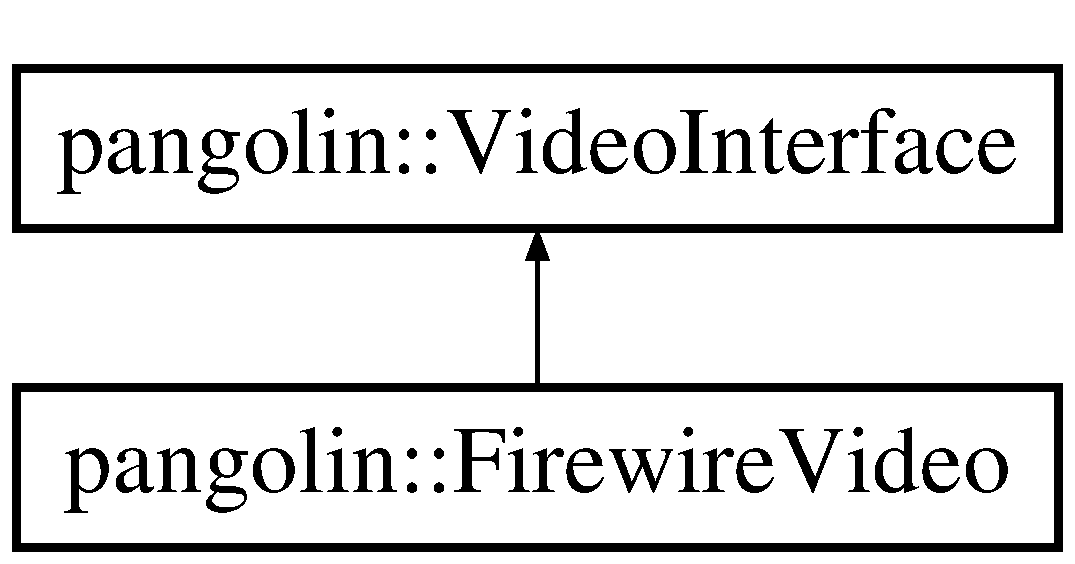
\includegraphics[height=2.000000cm]{classpangolin_1_1_firewire_video}
\end{center}
\end{figure}
\subsection*{Public Member Functions}
\begin{DoxyCompactItemize}
\item 
{\bfseries Firewire\+Video} (unsigned deviceid=0, dc1394video\+\_\+mode\+\_\+t video\+\_\+mode=D\+C1394\+\_\+\+V\+I\+D\+E\+O\+\_\+\+M\+O\+D\+E\+\_\+640x480\+\_\+\+R\+G\+B8, dc1394framerate\+\_\+t framerate=D\+C1394\+\_\+\+F\+R\+A\+M\+E\+R\+A\+T\+E\+\_\+30, dc1394speed\+\_\+t iso\+\_\+speed=D\+C1394\+\_\+\+I\+S\+O\+\_\+\+S\+P\+E\+E\+D\+\_\+400, int dma\+\_\+buffers=10)\hypertarget{classpangolin_1_1_firewire_video_adb5cdc5120ee7d80560a330497348cac}{}\label{classpangolin_1_1_firewire_video_adb5cdc5120ee7d80560a330497348cac}

\item 
{\bfseries Firewire\+Video} (\hyperlink{structpangolin_1_1_guid}{Guid} guid, dc1394video\+\_\+mode\+\_\+t video\+\_\+mode=D\+C1394\+\_\+\+V\+I\+D\+E\+O\+\_\+\+M\+O\+D\+E\+\_\+640x480\+\_\+\+R\+G\+B8, dc1394framerate\+\_\+t framerate=D\+C1394\+\_\+\+F\+R\+A\+M\+E\+R\+A\+T\+E\+\_\+30, dc1394speed\+\_\+t iso\+\_\+speed=D\+C1394\+\_\+\+I\+S\+O\+\_\+\+S\+P\+E\+E\+D\+\_\+400, int dma\+\_\+buffers=10)\hypertarget{classpangolin_1_1_firewire_video_a067ed2cd36ee9f09360c27eaff14b93f}{}\label{classpangolin_1_1_firewire_video_a067ed2cd36ee9f09360c27eaff14b93f}

\item 
{\bfseries Firewire\+Video} (\hyperlink{structpangolin_1_1_guid}{Guid} guid, dc1394video\+\_\+mode\+\_\+t video\+\_\+mode, float framerate, uint32\+\_\+t width, uint32\+\_\+t height, uint32\+\_\+t left, uint32\+\_\+t top, dc1394speed\+\_\+t iso\+\_\+speed, int dma\+\_\+buffers, bool reset\+\_\+at\+\_\+boot=false)\hypertarget{classpangolin_1_1_firewire_video_a7f7aa96fe8a8540c3ef0b38466d4bc4d}{}\label{classpangolin_1_1_firewire_video_a7f7aa96fe8a8540c3ef0b38466d4bc4d}

\item 
{\bfseries Firewire\+Video} (unsigned deviceid, dc1394video\+\_\+mode\+\_\+t video\+\_\+mode, float framerate, uint32\+\_\+t width, uint32\+\_\+t height, uint32\+\_\+t left, uint32\+\_\+t top, dc1394speed\+\_\+t iso\+\_\+speed, int dma\+\_\+buffers, bool reset\+\_\+at\+\_\+boot=false)\hypertarget{classpangolin_1_1_firewire_video_acf10f2f5ef3562ef67006b2a749f8d71}{}\label{classpangolin_1_1_firewire_video_acf10f2f5ef3562ef67006b2a749f8d71}

\item 
void \hyperlink{classpangolin_1_1_firewire_video_ad0c413432052a6f94141a6c075c4ed1d}{Start} ()\hypertarget{classpangolin_1_1_firewire_video_ad0c413432052a6f94141a6c075c4ed1d}{}\label{classpangolin_1_1_firewire_video_ad0c413432052a6f94141a6c075c4ed1d}

\begin{DoxyCompactList}\small\item\em Implement \hyperlink{structpangolin_1_1_video_input_a74a2e3e1b87c7cbf9de9bcb39e1df128}{Video\+Input\+::\+Start()} \end{DoxyCompactList}\item 
void \hyperlink{classpangolin_1_1_firewire_video_a67ddb48e5c653b0983a1f2d4b7a0faf9}{Stop} ()\hypertarget{classpangolin_1_1_firewire_video_a67ddb48e5c653b0983a1f2d4b7a0faf9}{}\label{classpangolin_1_1_firewire_video_a67ddb48e5c653b0983a1f2d4b7a0faf9}

\begin{DoxyCompactList}\small\item\em Implement \hyperlink{structpangolin_1_1_video_input_a8945f80194cc7ec9594db7f27e7d09b8}{Video\+Input\+::\+Stop()} \end{DoxyCompactList}\item 
size\+\_\+t \hyperlink{classpangolin_1_1_firewire_video_a32a6f8c93aed9120d5f540c4c69ca793}{Size\+Bytes} () const \hypertarget{classpangolin_1_1_firewire_video_a32a6f8c93aed9120d5f540c4c69ca793}{}\label{classpangolin_1_1_firewire_video_a32a6f8c93aed9120d5f540c4c69ca793}

\begin{DoxyCompactList}\small\item\em Implement \hyperlink{structpangolin_1_1_video_input_a93cee5c33386973a2a51165e6bdcf40b}{Video\+Input\+::\+Size\+Bytes()} \end{DoxyCompactList}\item 
const std\+::vector$<$ \hyperlink{classpangolin_1_1_stream_info}{Stream\+Info} $>$ \& \hyperlink{classpangolin_1_1_firewire_video_a7db0b959665fee03688cf0b9f5d3546f}{Streams} () const \hypertarget{classpangolin_1_1_firewire_video_a7db0b959665fee03688cf0b9f5d3546f}{}\label{classpangolin_1_1_firewire_video_a7db0b959665fee03688cf0b9f5d3546f}

\begin{DoxyCompactList}\small\item\em Implement \hyperlink{structpangolin_1_1_video_input_a9030d775d699c39ab7b7ba378c007c6a}{Video\+Input\+::\+Streams()} \end{DoxyCompactList}\item 
bool \hyperlink{classpangolin_1_1_firewire_video_ad42e74cface551b5242e1c9d72199902}{Grab\+Next} (unsigned char $\ast$image, bool wait=true)\hypertarget{classpangolin_1_1_firewire_video_ad42e74cface551b5242e1c9d72199902}{}\label{classpangolin_1_1_firewire_video_ad42e74cface551b5242e1c9d72199902}

\begin{DoxyCompactList}\small\item\em Implement \hyperlink{structpangolin_1_1_video_input_ad3d8ff59c1ec4139320097e6e1111f32}{Video\+Input\+::\+Grab\+Next()} \end{DoxyCompactList}\item 
bool \hyperlink{classpangolin_1_1_firewire_video_abcc320e89545f5225ef67cb1612bb742}{Grab\+Newest} (unsigned char $\ast$image, bool wait=true)\hypertarget{classpangolin_1_1_firewire_video_abcc320e89545f5225ef67cb1612bb742}{}\label{classpangolin_1_1_firewire_video_abcc320e89545f5225ef67cb1612bb742}

\begin{DoxyCompactList}\small\item\em Implement \hyperlink{structpangolin_1_1_video_input_a4c8ac38e3c6a3f591663aeebf645e4c6}{Video\+Input\+::\+Grab\+Newest()} \end{DoxyCompactList}\item 
unsigned \hyperlink{classpangolin_1_1_firewire_video_ad2b14b1381aeb2375345992a60bec851}{Width} () const \hypertarget{classpangolin_1_1_firewire_video_ad2b14b1381aeb2375345992a60bec851}{}\label{classpangolin_1_1_firewire_video_ad2b14b1381aeb2375345992a60bec851}

\begin{DoxyCompactList}\small\item\em (deprecated\+: use Streams\mbox{[}i\mbox{]}.\hyperlink{classpangolin_1_1_firewire_video_ad2b14b1381aeb2375345992a60bec851}{Width()}) Return image width \end{DoxyCompactList}\item 
unsigned \hyperlink{classpangolin_1_1_firewire_video_a2c7695e31533bda8c63931946e64c7b0}{Height} () const \hypertarget{classpangolin_1_1_firewire_video_a2c7695e31533bda8c63931946e64c7b0}{}\label{classpangolin_1_1_firewire_video_a2c7695e31533bda8c63931946e64c7b0}

\begin{DoxyCompactList}\small\item\em (deprecated\+: use Streams\mbox{[}i\mbox{]}.\hyperlink{classpangolin_1_1_firewire_video_a2c7695e31533bda8c63931946e64c7b0}{Height()}) Return image height \end{DoxyCompactList}\item 
\hyperlink{classpangolin_1_1_firewire_frame}{Firewire\+Frame} \hyperlink{classpangolin_1_1_firewire_video_a7166bc530dfac2362956761f34e73436}{Get\+Next} (bool wait=true)
\begin{DoxyCompactList}\small\item\em Return object containing reference to image data within D\+MA buffer. \end{DoxyCompactList}\item 
\hyperlink{classpangolin_1_1_firewire_frame}{Firewire\+Frame} \hyperlink{classpangolin_1_1_firewire_video_adad292fb68e0f81c97817b249a4ba032}{Get\+Newest} (bool wait=true)
\begin{DoxyCompactList}\small\item\em Return object containing reference to newest image data within D\+MA buffer discarding old images. \end{DoxyCompactList}\item 
void \hyperlink{classpangolin_1_1_firewire_video_a67697c233b215e2653b291fa91819a2c}{Put\+Frame} (\hyperlink{classpangolin_1_1_firewire_frame}{Firewire\+Frame} \&frame)
\begin{DoxyCompactList}\small\item\em Return \hyperlink{classpangolin_1_1_firewire_frame}{Firewire\+Frame} object. \end{DoxyCompactList}\item 
float \hyperlink{classpangolin_1_1_firewire_video_a407d7d270893d7d2e137867f0bf4859c}{Get\+Shutter\+Time} () const \hypertarget{classpangolin_1_1_firewire_video_a407d7d270893d7d2e137867f0bf4859c}{}\label{classpangolin_1_1_firewire_video_a407d7d270893d7d2e137867f0bf4859c}

\begin{DoxyCompactList}\small\item\em return absolute shutter value \end{DoxyCompactList}\item 
void \hyperlink{classpangolin_1_1_firewire_video_a9eb2207c6ff877e7f7c466795fad1370}{Set\+Shutter\+Time} (float val)\hypertarget{classpangolin_1_1_firewire_video_a9eb2207c6ff877e7f7c466795fad1370}{}\label{classpangolin_1_1_firewire_video_a9eb2207c6ff877e7f7c466795fad1370}

\begin{DoxyCompactList}\small\item\em set absolute shutter value \end{DoxyCompactList}\item 
void \hyperlink{classpangolin_1_1_firewire_video_a4bf719eea88bbcfb44ec11faab76284b}{Set\+Auto\+Shutter\+Time} ()\hypertarget{classpangolin_1_1_firewire_video_a4bf719eea88bbcfb44ec11faab76284b}{}\label{classpangolin_1_1_firewire_video_a4bf719eea88bbcfb44ec11faab76284b}

\begin{DoxyCompactList}\small\item\em set auto shutter value \end{DoxyCompactList}\item 
float \hyperlink{classpangolin_1_1_firewire_video_a14ca55a65145e773375dfdddf70eab77}{Get\+Gain} () const \hypertarget{classpangolin_1_1_firewire_video_a14ca55a65145e773375dfdddf70eab77}{}\label{classpangolin_1_1_firewire_video_a14ca55a65145e773375dfdddf70eab77}

\begin{DoxyCompactList}\small\item\em return absolute gain value \end{DoxyCompactList}\item 
void \hyperlink{classpangolin_1_1_firewire_video_afec9844474a565b160a5afb403f3e10b}{Set\+Gain} (float val)\hypertarget{classpangolin_1_1_firewire_video_afec9844474a565b160a5afb403f3e10b}{}\label{classpangolin_1_1_firewire_video_afec9844474a565b160a5afb403f3e10b}

\begin{DoxyCompactList}\small\item\em set absolute gain value \end{DoxyCompactList}\item 
void \hyperlink{classpangolin_1_1_firewire_video_ada36a8dc9be7e59f5c1923b9ff36da70}{Set\+Auto\+Gain} ()\hypertarget{classpangolin_1_1_firewire_video_ada36a8dc9be7e59f5c1923b9ff36da70}{}\label{classpangolin_1_1_firewire_video_ada36a8dc9be7e59f5c1923b9ff36da70}

\begin{DoxyCompactList}\small\item\em set auto gain value \end{DoxyCompactList}\item 
float \hyperlink{classpangolin_1_1_firewire_video_af355639475469981cb15b4390d266262}{Get\+Brightness} () const \hypertarget{classpangolin_1_1_firewire_video_af355639475469981cb15b4390d266262}{}\label{classpangolin_1_1_firewire_video_af355639475469981cb15b4390d266262}

\begin{DoxyCompactList}\small\item\em return absolute brightness value \end{DoxyCompactList}\item 
void \hyperlink{classpangolin_1_1_firewire_video_af213a0ee97d016a4bfafb6329df4c547}{Set\+Brightness} (float val)\hypertarget{classpangolin_1_1_firewire_video_af213a0ee97d016a4bfafb6329df4c547}{}\label{classpangolin_1_1_firewire_video_af213a0ee97d016a4bfafb6329df4c547}

\begin{DoxyCompactList}\small\item\em set absolute brightness value \end{DoxyCompactList}\item 
void \hyperlink{classpangolin_1_1_firewire_video_acf26771d0af047032ab1868c0baa53a2}{Set\+Auto\+Brightness} ()\hypertarget{classpangolin_1_1_firewire_video_acf26771d0af047032ab1868c0baa53a2}{}\label{classpangolin_1_1_firewire_video_acf26771d0af047032ab1868c0baa53a2}

\begin{DoxyCompactList}\small\item\em set auto brightness \end{DoxyCompactList}\item 
float \hyperlink{classpangolin_1_1_firewire_video_a12e5808fd5816410e271bf881645efd1}{Get\+Gamma} () const \hypertarget{classpangolin_1_1_firewire_video_a12e5808fd5816410e271bf881645efd1}{}\label{classpangolin_1_1_firewire_video_a12e5808fd5816410e271bf881645efd1}

\begin{DoxyCompactList}\small\item\em return absolute gamma value \end{DoxyCompactList}\item 
void \hyperlink{classpangolin_1_1_firewire_video_a9f967e437cfaccc8b5464d4c80f88d4b}{Set\+Shutter\+Time\+Quant} (int shutter)\hypertarget{classpangolin_1_1_firewire_video_a9f967e437cfaccc8b5464d4c80f88d4b}{}\label{classpangolin_1_1_firewire_video_a9f967e437cfaccc8b5464d4c80f88d4b}

\begin{DoxyCompactList}\small\item\em return quantised shutter value \end{DoxyCompactList}\item 
void \hyperlink{classpangolin_1_1_firewire_video_ac375b0f8d679540024551bc519a9c5b7}{Set\+Internal\+Trigger} ()\hypertarget{classpangolin_1_1_firewire_video_ac375b0f8d679540024551bc519a9c5b7}{}\label{classpangolin_1_1_firewire_video_ac375b0f8d679540024551bc519a9c5b7}

\begin{DoxyCompactList}\small\item\em set the trigger to internal, i.\+e. determined by video mode \end{DoxyCompactList}\item 
void \hyperlink{classpangolin_1_1_firewire_video_a9afb190bea29b973da13be399793fb97}{Set\+External\+Trigger} (dc1394trigger\+\_\+mode\+\_\+t mode=D\+C1394\+\_\+\+T\+R\+I\+G\+G\+E\+R\+\_\+\+M\+O\+D\+E\+\_\+0, dc1394trigger\+\_\+polarity\+\_\+t polarity=D\+C1394\+\_\+\+T\+R\+I\+G\+G\+E\+R\+\_\+\+A\+C\+T\+I\+V\+E\+\_\+\+H\+I\+GH, dc1394trigger\+\_\+source\+\_\+t source=D\+C1394\+\_\+\+T\+R\+I\+G\+G\+E\+R\+\_\+\+S\+O\+U\+R\+C\+E\+\_\+0)\hypertarget{classpangolin_1_1_firewire_video_a9afb190bea29b973da13be399793fb97}{}\label{classpangolin_1_1_firewire_video_a9afb190bea29b973da13be399793fb97}

\begin{DoxyCompactList}\small\item\em set the trigger to external \end{DoxyCompactList}\item 
void \hyperlink{classpangolin_1_1_firewire_video_a8099ff483fdb5249f2c7ecf59135e2d9}{Set\+Register} (uint64\+\_\+t offset, uint32\+\_\+t value)\hypertarget{classpangolin_1_1_firewire_video_a8099ff483fdb5249f2c7ecf59135e2d9}{}\label{classpangolin_1_1_firewire_video_a8099ff483fdb5249f2c7ecf59135e2d9}

\begin{DoxyCompactList}\small\item\em set a camera register \end{DoxyCompactList}\item 
uint32\+\_\+t \hyperlink{classpangolin_1_1_firewire_video_ace2a55a3061f3f6567fbf65d9fe80cea}{Get\+Register} (uint64\+\_\+t offset)\hypertarget{classpangolin_1_1_firewire_video_ace2a55a3061f3f6567fbf65d9fe80cea}{}\label{classpangolin_1_1_firewire_video_ace2a55a3061f3f6567fbf65d9fe80cea}

\begin{DoxyCompactList}\small\item\em read camera register \end{DoxyCompactList}\item 
void \hyperlink{classpangolin_1_1_firewire_video_a7015ff3b7ab687d45cd8283c4081cd4e}{Set\+Control\+Register} (uint64\+\_\+t offset, uint32\+\_\+t value)\hypertarget{classpangolin_1_1_firewire_video_a7015ff3b7ab687d45cd8283c4081cd4e}{}\label{classpangolin_1_1_firewire_video_a7015ff3b7ab687d45cd8283c4081cd4e}

\begin{DoxyCompactList}\small\item\em set a camera control register \end{DoxyCompactList}\item 
uint32\+\_\+t \hyperlink{classpangolin_1_1_firewire_video_a98257feba91833cb43eb899a35b7c036}{Get\+Control\+Register} (uint64\+\_\+t offset)\hypertarget{classpangolin_1_1_firewire_video_a98257feba91833cb43eb899a35b7c036}{}\label{classpangolin_1_1_firewire_video_a98257feba91833cb43eb899a35b7c036}

\begin{DoxyCompactList}\small\item\em read camera control register \end{DoxyCompactList}\end{DoxyCompactItemize}
\subsection*{Static Public Attributes}
\begin{DoxyCompactItemize}
\item 
static const int {\bfseries M\+A\+X\+\_\+\+FR} = -\/1\hypertarget{classpangolin_1_1_firewire_video_a0ce79c1df497e71c022fe9919713e5af}{}\label{classpangolin_1_1_firewire_video_a0ce79c1df497e71c022fe9919713e5af}

\item 
static const int {\bfseries E\+X\+T\+\_\+\+T\+R\+IG} = -\/1\hypertarget{classpangolin_1_1_firewire_video_aea2debb6123acf1d1ceefeeb0663f04c}{}\label{classpangolin_1_1_firewire_video_aea2debb6123acf1d1ceefeeb0663f04c}

\item 
static const uint32\+\_\+t {\bfseries G\+P\+I\+O\+\_\+\+C\+T\+R\+L\+\_\+\+P\+I\+N0} = 0x1110\hypertarget{classpangolin_1_1_firewire_video_a2e5e177ea31dd40acfd518c79e53c246}{}\label{classpangolin_1_1_firewire_video_a2e5e177ea31dd40acfd518c79e53c246}

\item 
static const uint32\+\_\+t {\bfseries G\+P\+I\+O\+\_\+\+C\+T\+R\+L\+\_\+\+P\+I\+N1} = 0x1120\hypertarget{classpangolin_1_1_firewire_video_ad2983819408781dcecc1d8be4b3a4f3f}{}\label{classpangolin_1_1_firewire_video_ad2983819408781dcecc1d8be4b3a4f3f}

\item 
static const uint32\+\_\+t {\bfseries G\+P\+I\+O\+\_\+\+C\+T\+R\+L\+\_\+\+P\+I\+N2} = 0x1130\hypertarget{classpangolin_1_1_firewire_video_aeba42568a56d4b049308d2af68d9ea9d}{}\label{classpangolin_1_1_firewire_video_aeba42568a56d4b049308d2af68d9ea9d}

\item 
static const uint32\+\_\+t {\bfseries G\+P\+I\+O\+\_\+\+C\+T\+R\+L\+\_\+\+P\+I\+N3} = 0x1140\hypertarget{classpangolin_1_1_firewire_video_a62d1a598f80a69265f5d84a211410353}{}\label{classpangolin_1_1_firewire_video_a62d1a598f80a69265f5d84a211410353}

\end{DoxyCompactItemize}
\subsection*{Protected Member Functions}
\begin{DoxyCompactItemize}
\item 
void {\bfseries init\+\_\+stream\+\_\+info} ()\hypertarget{classpangolin_1_1_firewire_video_af566d3aa8b37cdeb11e31f8be52e6021}{}\label{classpangolin_1_1_firewire_video_af566d3aa8b37cdeb11e31f8be52e6021}

\item 
void {\bfseries init\+\_\+camera} (uint64\+\_\+t guid, int dma\+\_\+frames, dc1394speed\+\_\+t iso\+\_\+speed, dc1394video\+\_\+mode\+\_\+t video\+\_\+mode, dc1394framerate\+\_\+t framerate)\hypertarget{classpangolin_1_1_firewire_video_a65a81792a5108644a08053f57a7f4f36}{}\label{classpangolin_1_1_firewire_video_a65a81792a5108644a08053f57a7f4f36}

\item 
void {\bfseries init\+\_\+format7\+\_\+camera} (uint64\+\_\+t guid, int dma\+\_\+frames, dc1394speed\+\_\+t iso\+\_\+speed, dc1394video\+\_\+mode\+\_\+t video\+\_\+mode, float framerate, uint32\+\_\+t width, uint32\+\_\+t height, uint32\+\_\+t left, uint32\+\_\+t top, bool reset\+\_\+at\+\_\+boot)\hypertarget{classpangolin_1_1_firewire_video_a9941c6915a9d099a09a90c0ee4f8889f}{}\label{classpangolin_1_1_firewire_video_a9941c6915a9d099a09a90c0ee4f8889f}

\end{DoxyCompactItemize}
\subsection*{Static Protected Member Functions}
\begin{DoxyCompactItemize}
\item 
static int {\bfseries nearest\+\_\+value} (int value, int step, int min, int max)\hypertarget{classpangolin_1_1_firewire_video_ac6ae940b361f0a33757bb420fcd5d2fa}{}\label{classpangolin_1_1_firewire_video_ac6ae940b361f0a33757bb420fcd5d2fa}

\item 
static double {\bfseries bus\+\_\+period\+\_\+from\+\_\+iso\+\_\+speed} (dc1394speed\+\_\+t iso\+\_\+speed)\hypertarget{classpangolin_1_1_firewire_video_a566c1d07d6539ebbfbb11cf567f69fb0}{}\label{classpangolin_1_1_firewire_video_a566c1d07d6539ebbfbb11cf567f69fb0}

\end{DoxyCompactItemize}
\subsection*{Protected Attributes}
\begin{DoxyCompactItemize}
\item 
size\+\_\+t {\bfseries frame\+\_\+size\+\_\+bytes}\hypertarget{classpangolin_1_1_firewire_video_aff8ee169586212bd7fc169c561b03326}{}\label{classpangolin_1_1_firewire_video_aff8ee169586212bd7fc169c561b03326}

\item 
std\+::vector$<$ \hyperlink{classpangolin_1_1_stream_info}{Stream\+Info} $>$ {\bfseries streams}\hypertarget{classpangolin_1_1_firewire_video_a89332a71bec0c9f204607016f1bd935d}{}\label{classpangolin_1_1_firewire_video_a89332a71bec0c9f204607016f1bd935d}

\item 
bool {\bfseries running}\hypertarget{classpangolin_1_1_firewire_video_ac2ccdc08d1f8fbb010699b83aa09e8fe}{}\label{classpangolin_1_1_firewire_video_ac2ccdc08d1f8fbb010699b83aa09e8fe}

\item 
dc1394camera\+\_\+t $\ast$ {\bfseries camera}\hypertarget{classpangolin_1_1_firewire_video_abcae4260a8bc674768a68a529a2b4319}{}\label{classpangolin_1_1_firewire_video_abcae4260a8bc674768a68a529a2b4319}

\item 
unsigned {\bfseries width}\hypertarget{classpangolin_1_1_firewire_video_a63d384d116e6fe3c02b804918a87c84e}{}\label{classpangolin_1_1_firewire_video_a63d384d116e6fe3c02b804918a87c84e}

\item 
unsigned {\bfseries height}\hypertarget{classpangolin_1_1_firewire_video_a67a0e6a1adf91634ab9113ead4d00eea}{}\label{classpangolin_1_1_firewire_video_a67a0e6a1adf91634ab9113ead4d00eea}

\item 
unsigned {\bfseries top}\hypertarget{classpangolin_1_1_firewire_video_a9e678e2775cb145d048397e300fe8e48}{}\label{classpangolin_1_1_firewire_video_a9e678e2775cb145d048397e300fe8e48}

\item 
unsigned {\bfseries left}\hypertarget{classpangolin_1_1_firewire_video_abe132e99aff12b3919c13467380b2d25}{}\label{classpangolin_1_1_firewire_video_abe132e99aff12b3919c13467380b2d25}

\item 
dc1394\+\_\+t $\ast$ {\bfseries d}\hypertarget{classpangolin_1_1_firewire_video_a72729c15c02a55e2642baf081a6fa02c}{}\label{classpangolin_1_1_firewire_video_a72729c15c02a55e2642baf081a6fa02c}

\item 
dc1394camera\+\_\+list\+\_\+t $\ast$ {\bfseries list}\hypertarget{classpangolin_1_1_firewire_video_a4896572c521a2e7d0ef33ee931cb10e6}{}\label{classpangolin_1_1_firewire_video_a4896572c521a2e7d0ef33ee931cb10e6}

\item 
dc1394error\+\_\+t {\bfseries err}\hypertarget{classpangolin_1_1_firewire_video_ad1e18e5197391f71b90ecb27ba49e597}{}\label{classpangolin_1_1_firewire_video_ad1e18e5197391f71b90ecb27ba49e597}

\end{DoxyCompactItemize}


\subsection{Member Function Documentation}
\index{pangolin\+::\+Firewire\+Video@{pangolin\+::\+Firewire\+Video}!Get\+Newest@{Get\+Newest}}
\index{Get\+Newest@{Get\+Newest}!pangolin\+::\+Firewire\+Video@{pangolin\+::\+Firewire\+Video}}
\subsubsection[{\texorpdfstring{Get\+Newest(bool wait=true)}{GetNewest(bool wait=true)}}]{\setlength{\rightskip}{0pt plus 5cm}{\bf Firewire\+Frame} pangolin\+::\+Firewire\+Video\+::\+Get\+Newest (
\begin{DoxyParamCaption}
\item[{bool}]{wait = {\ttfamily true}}
\end{DoxyParamCaption}
)}\hypertarget{classpangolin_1_1_firewire_video_adad292fb68e0f81c97817b249a4ba032}{}\label{classpangolin_1_1_firewire_video_adad292fb68e0f81c97817b249a4ba032}


Return object containing reference to newest image data within D\+MA buffer discarding old images. 

The \hyperlink{classpangolin_1_1_firewire_frame}{Firewire\+Frame} must be returned to signal that it can be reused with a corresponding \hyperlink{classpangolin_1_1_firewire_video_a67697c233b215e2653b291fa91819a2c}{Put\+Frame()} \index{pangolin\+::\+Firewire\+Video@{pangolin\+::\+Firewire\+Video}!Get\+Next@{Get\+Next}}
\index{Get\+Next@{Get\+Next}!pangolin\+::\+Firewire\+Video@{pangolin\+::\+Firewire\+Video}}
\subsubsection[{\texorpdfstring{Get\+Next(bool wait=true)}{GetNext(bool wait=true)}}]{\setlength{\rightskip}{0pt plus 5cm}{\bf Firewire\+Frame} pangolin\+::\+Firewire\+Video\+::\+Get\+Next (
\begin{DoxyParamCaption}
\item[{bool}]{wait = {\ttfamily true}}
\end{DoxyParamCaption}
)}\hypertarget{classpangolin_1_1_firewire_video_a7166bc530dfac2362956761f34e73436}{}\label{classpangolin_1_1_firewire_video_a7166bc530dfac2362956761f34e73436}


Return object containing reference to image data within D\+MA buffer. 

The \hyperlink{classpangolin_1_1_firewire_frame}{Firewire\+Frame} must be returned to signal that it can be reused with a corresponding \hyperlink{classpangolin_1_1_firewire_video_a67697c233b215e2653b291fa91819a2c}{Put\+Frame()} \index{pangolin\+::\+Firewire\+Video@{pangolin\+::\+Firewire\+Video}!Put\+Frame@{Put\+Frame}}
\index{Put\+Frame@{Put\+Frame}!pangolin\+::\+Firewire\+Video@{pangolin\+::\+Firewire\+Video}}
\subsubsection[{\texorpdfstring{Put\+Frame(\+Firewire\+Frame \&frame)}{PutFrame(FirewireFrame &frame)}}]{\setlength{\rightskip}{0pt plus 5cm}void pangolin\+::\+Firewire\+Video\+::\+Put\+Frame (
\begin{DoxyParamCaption}
\item[{{\bf Firewire\+Frame} \&}]{frame}
\end{DoxyParamCaption}
)}\hypertarget{classpangolin_1_1_firewire_video_a67697c233b215e2653b291fa91819a2c}{}\label{classpangolin_1_1_firewire_video_a67697c233b215e2653b291fa91819a2c}


Return \hyperlink{classpangolin_1_1_firewire_frame}{Firewire\+Frame} object. 

Data held by \hyperlink{classpangolin_1_1_firewire_frame}{Firewire\+Frame} is invalidated on return. 

The documentation for this class was generated from the following file\+:\begin{DoxyCompactItemize}
\item 
/home/gapo/meng/deps/pangolin/include/pangolin/video/drivers/firewire.\+h\end{DoxyCompactItemize}

\hypertarget{structpangolin_1_1_frame_input}{}\section{pangolin\+:\+:Frame\+Input Struct Reference}
\label{structpangolin_1_1_frame_input}\index{pangolin\+::\+Frame\+Input@{pangolin\+::\+Frame\+Input}}
\subsection*{Public Attributes}
\begin{DoxyCompactItemize}
\item 
int {\bfseries index}\hypertarget{structpangolin_1_1_frame_input_a59ff81a76f8088ac7123bd944c59ebd1}{}\label{structpangolin_1_1_frame_input_a59ff81a76f8088ac7123bd944c59ebd1}

\item 
std\+::string {\bfseries var}\hypertarget{structpangolin_1_1_frame_input_ab05c7f034c74c2de7712671961944456}{}\label{structpangolin_1_1_frame_input_ab05c7f034c74c2de7712671961944456}

\item 
std\+::string {\bfseries val}\hypertarget{structpangolin_1_1_frame_input_a5efcc26257d1585fc27b46c57deb90f4}{}\label{structpangolin_1_1_frame_input_a5efcc26257d1585fc27b46c57deb90f4}

\end{DoxyCompactItemize}


The documentation for this struct was generated from the following file\+:\begin{DoxyCompactItemize}
\item 
/home/gapo/meng/deps/pangolin/include/pangolin/var/input\+\_\+record\+\_\+repeat.\+h\end{DoxyCompactItemize}

\hypertarget{structpangolin_1_1_gl_buffer}{}\section{pangolin\+:\+:Gl\+Buffer Struct Reference}
\label{structpangolin_1_1_gl_buffer}\index{pangolin\+::\+Gl\+Buffer@{pangolin\+::\+Gl\+Buffer}}
Inheritance diagram for pangolin\+:\+:Gl\+Buffer\+:\begin{figure}[H]
\begin{center}
\leavevmode
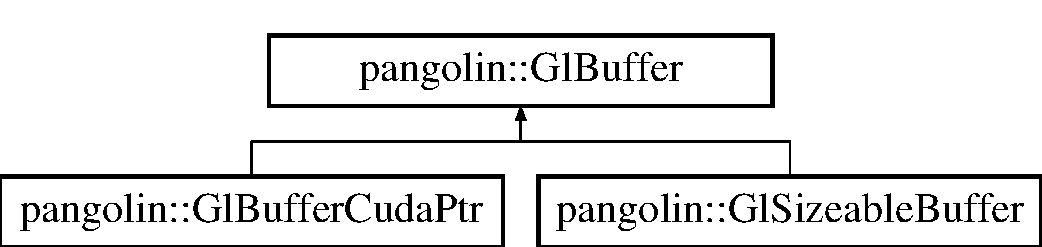
\includegraphics[height=2.000000cm]{structpangolin_1_1_gl_buffer}
\end{center}
\end{figure}
\subsection*{Public Member Functions}
\begin{DoxyCompactItemize}
\item 
\hyperlink{structpangolin_1_1_gl_buffer_a79a7e18ccfd8fc65b92d12729e387190}{Gl\+Buffer} ()\hypertarget{structpangolin_1_1_gl_buffer_a79a7e18ccfd8fc65b92d12729e387190}{}\label{structpangolin_1_1_gl_buffer_a79a7e18ccfd8fc65b92d12729e387190}

\begin{DoxyCompactList}\small\item\em Default constructor represents \textquotesingle{}no buffer\textquotesingle{}. \end{DoxyCompactList}\item 
{\bfseries Gl\+Buffer} (Gl\+Buffer\+Type buffer\+\_\+type, G\+Luint num\+\_\+elements, G\+Lenum datatype, G\+Luint count\+\_\+per\+\_\+element, G\+Lenum gluse=G\+L\+\_\+\+D\+Y\+N\+A\+M\+I\+C\+\_\+\+D\+R\+AW)\hypertarget{structpangolin_1_1_gl_buffer_a4d7733b41cc4aa26af87c9d9b2302438}{}\label{structpangolin_1_1_gl_buffer_a4d7733b41cc4aa26af87c9d9b2302438}

\item 
bool {\bfseries Is\+Valid} () const \hypertarget{structpangolin_1_1_gl_buffer_a5a5f4090406297c55ec7db7427927824}{}\label{structpangolin_1_1_gl_buffer_a5a5f4090406297c55ec7db7427927824}

\item 
void {\bfseries Reinitialise} (Gl\+Buffer\+Type buffer\+\_\+type, G\+Luint num\+\_\+elements, G\+Lenum datatype, G\+Luint count\+\_\+per\+\_\+element, G\+Lenum gluse)\hypertarget{structpangolin_1_1_gl_buffer_a9d2b5477723741351b611225a59f096d}{}\label{structpangolin_1_1_gl_buffer_a9d2b5477723741351b611225a59f096d}

\item 
void {\bfseries Resize} (G\+Luint num\+\_\+elements)\hypertarget{structpangolin_1_1_gl_buffer_aed1fa9ab25b4ade2e4c5dbd19e7f1dde}{}\label{structpangolin_1_1_gl_buffer_aed1fa9ab25b4ade2e4c5dbd19e7f1dde}

\item 
void {\bfseries Bind} () const \hypertarget{structpangolin_1_1_gl_buffer_aa2daa9a7a43e70ffbab240299bec5b08}{}\label{structpangolin_1_1_gl_buffer_aa2daa9a7a43e70ffbab240299bec5b08}

\item 
void {\bfseries Unbind} () const \hypertarget{structpangolin_1_1_gl_buffer_ad4a2d1ceb35fd1b319b0d288af6f2466}{}\label{structpangolin_1_1_gl_buffer_ad4a2d1ceb35fd1b319b0d288af6f2466}

\item 
void {\bfseries Upload} (const G\+Lvoid $\ast$data, G\+Lsizeiptr size\+\_\+bytes, G\+Lintptr offset=0)\hypertarget{structpangolin_1_1_gl_buffer_a4bb774712e15e148c4e721e1466f3144}{}\label{structpangolin_1_1_gl_buffer_a4bb774712e15e148c4e721e1466f3144}

\end{DoxyCompactItemize}
\subsection*{Public Attributes}
\begin{DoxyCompactItemize}
\item 
G\+Luint {\bfseries bo}\hypertarget{structpangolin_1_1_gl_buffer_adcae774cc3075a7427acb7e78c1dcc70}{}\label{structpangolin_1_1_gl_buffer_adcae774cc3075a7427acb7e78c1dcc70}

\item 
Gl\+Buffer\+Type {\bfseries buffer\+\_\+type}\hypertarget{structpangolin_1_1_gl_buffer_a49d82803f478868af7438a5940b309b7}{}\label{structpangolin_1_1_gl_buffer_a49d82803f478868af7438a5940b309b7}

\item 
G\+Lenum {\bfseries gluse}\hypertarget{structpangolin_1_1_gl_buffer_ae76ae84e7814c1fad5321fdc0ba7e305}{}\label{structpangolin_1_1_gl_buffer_ae76ae84e7814c1fad5321fdc0ba7e305}

\item 
G\+Lenum {\bfseries datatype}\hypertarget{structpangolin_1_1_gl_buffer_aa158b6b9111ae907d30618953f91cefb}{}\label{structpangolin_1_1_gl_buffer_aa158b6b9111ae907d30618953f91cefb}

\item 
G\+Luint {\bfseries num\+\_\+elements}\hypertarget{structpangolin_1_1_gl_buffer_adca05c7ac6309f4a8e06f58cda9fb6b1}{}\label{structpangolin_1_1_gl_buffer_adca05c7ac6309f4a8e06f58cda9fb6b1}

\item 
G\+Luint {\bfseries count\+\_\+per\+\_\+element}\hypertarget{structpangolin_1_1_gl_buffer_a4070d916da45cc9ce08d853dee9cbf7f}{}\label{structpangolin_1_1_gl_buffer_a4070d916da45cc9ce08d853dee9cbf7f}

\end{DoxyCompactItemize}


The documentation for this struct was generated from the following file\+:\begin{DoxyCompactItemize}
\item 
/home/gapo/meng/deps/pangolin/include/pangolin/gl/gl.\+h\end{DoxyCompactItemize}

\hypertarget{structpangolin_1_1_gl_buffer_cuda_ptr}{}\section{pangolin\+:\+:Gl\+Buffer\+Cuda\+Ptr Struct Reference}
\label{structpangolin_1_1_gl_buffer_cuda_ptr}\index{pangolin\+::\+Gl\+Buffer\+Cuda\+Ptr@{pangolin\+::\+Gl\+Buffer\+Cuda\+Ptr}}
Inheritance diagram for pangolin\+:\+:Gl\+Buffer\+Cuda\+Ptr\+:\begin{figure}[H]
\begin{center}
\leavevmode
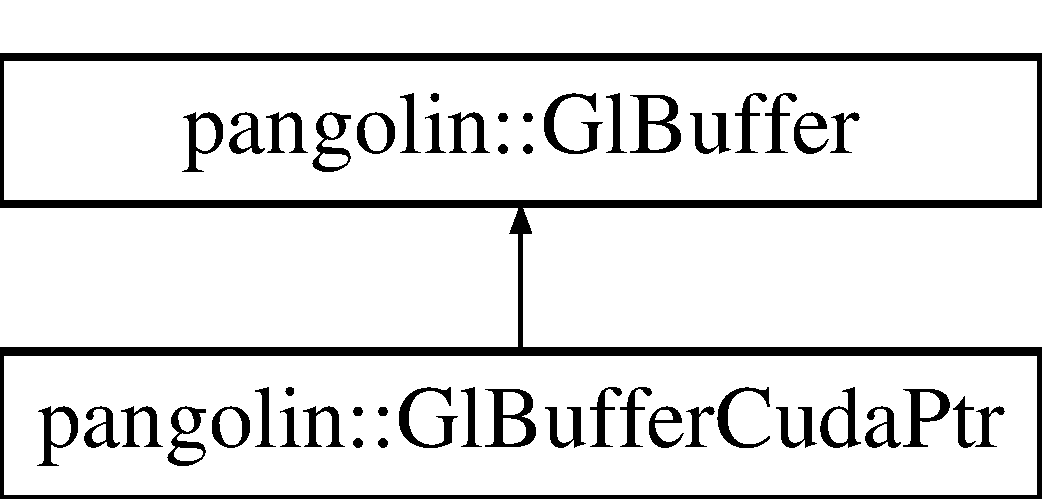
\includegraphics[height=2.000000cm]{structpangolin_1_1_gl_buffer_cuda_ptr}
\end{center}
\end{figure}
\subsection*{Public Member Functions}
\begin{DoxyCompactItemize}
\item 
\hyperlink{structpangolin_1_1_gl_buffer_cuda_ptr_ac9b4a41fd4bfb92681aabe0220ae4c19}{Gl\+Buffer\+Cuda\+Ptr} ()\hypertarget{structpangolin_1_1_gl_buffer_cuda_ptr_ac9b4a41fd4bfb92681aabe0220ae4c19}{}\label{structpangolin_1_1_gl_buffer_cuda_ptr_ac9b4a41fd4bfb92681aabe0220ae4c19}

\begin{DoxyCompactList}\small\item\em Default constructor represents \textquotesingle{}no buffer\textquotesingle{}. \end{DoxyCompactList}\item 
{\bfseries Gl\+Buffer\+Cuda\+Ptr} (Gl\+Buffer\+Type buffer\+\_\+type, G\+Luint size\+\_\+bytes, unsigned int cudause, G\+Lenum gluse)\hypertarget{structpangolin_1_1_gl_buffer_cuda_ptr_a6a8eb4364a76bf152cf718db243d74b0}{}\label{structpangolin_1_1_gl_buffer_cuda_ptr_a6a8eb4364a76bf152cf718db243d74b0}

\item 
{\bfseries Gl\+Buffer\+Cuda\+Ptr} (Gl\+Buffer\+Type buffer\+\_\+type, G\+Luint num\+\_\+elements, G\+Lenum datatype, G\+Luint count\+\_\+per\+\_\+element, unsigned int cudause, G\+Lenum gluse)\hypertarget{structpangolin_1_1_gl_buffer_cuda_ptr_a43ea7966e05f24fa3ee1f4b108c66da0}{}\label{structpangolin_1_1_gl_buffer_cuda_ptr_a43ea7966e05f24fa3ee1f4b108c66da0}

\item 
P\+A\+N\+G\+O\+L\+I\+N\+\_\+\+D\+E\+P\+R\+E\+C\+A\+T\+ED {\bfseries Gl\+Buffer\+Cuda\+Ptr} (Gl\+Buffer\+Type buffer\+\_\+type, G\+Luint width, G\+Luint height, G\+Lenum datatype, G\+Luint count\+\_\+per\+\_\+element, unsigned int cudause, G\+Lenum gluse)\hypertarget{structpangolin_1_1_gl_buffer_cuda_ptr_a04776a32826133907613cf85956e6596}{}\label{structpangolin_1_1_gl_buffer_cuda_ptr_a04776a32826133907613cf85956e6596}

\item 
void {\bfseries Reinitialise} (Gl\+Buffer\+Type buffer\+\_\+type, G\+Luint size\+\_\+bytes, unsigned int cudause, G\+Lenum gluse)\hypertarget{structpangolin_1_1_gl_buffer_cuda_ptr_a8839c7255c48aff5f83144aca20369d0}{}\label{structpangolin_1_1_gl_buffer_cuda_ptr_a8839c7255c48aff5f83144aca20369d0}

\item 
void {\bfseries Reinitialise} (Gl\+Buffer\+Type buffer\+\_\+type, G\+Luint num\+\_\+elements, G\+Lenum datatype, G\+Luint count\+\_\+per\+\_\+element, unsigned int cudause, G\+Lenum gluse)\hypertarget{structpangolin_1_1_gl_buffer_cuda_ptr_a8bb960c4b57ba1b67a6556ff7a8dd645}{}\label{structpangolin_1_1_gl_buffer_cuda_ptr_a8bb960c4b57ba1b67a6556ff7a8dd645}

\end{DoxyCompactItemize}
\subsection*{Public Attributes}
\begin{DoxyCompactItemize}
\item 
cuda\+Graphics\+Resource $\ast$ {\bfseries cuda\+\_\+res}\hypertarget{structpangolin_1_1_gl_buffer_cuda_ptr_a9c2198ee3178205fb6a704cbf2d42ff5}{}\label{structpangolin_1_1_gl_buffer_cuda_ptr_a9c2198ee3178205fb6a704cbf2d42ff5}

\end{DoxyCompactItemize}


The documentation for this struct was generated from the following file\+:\begin{DoxyCompactItemize}
\item 
/home/gapo/meng/deps/pangolin/include/pangolin/gl/glcuda.\+h\end{DoxyCompactItemize}

\hypertarget{classpangolin_1_1_gl_char}{}\section{pangolin\+:\+:Gl\+Char Class Reference}
\label{classpangolin_1_1_gl_char}\index{pangolin\+::\+Gl\+Char@{pangolin\+::\+Gl\+Char}}
\subsection*{Public Member Functions}
\begin{DoxyCompactItemize}
\item 
{\bfseries Gl\+Char} (int tw, int th, int x, int y, int w, int h, G\+Lfloat x\+\_\+step, G\+Lfloat ox, G\+Lfloat oy)\hypertarget{classpangolin_1_1_gl_char_a3a0248ed0d062da8591e61c1063d9d67}{}\label{classpangolin_1_1_gl_char_a3a0248ed0d062da8591e61c1063d9d67}

\item 
const \hyperlink{structpangolin_1_1_x_y_u_v}{X\+Y\+UV} \& {\bfseries Get\+Vert} (size\+\_\+t i) const \hypertarget{classpangolin_1_1_gl_char_a5fdd81d07442e6a23d17710c683f0d6f}{}\label{classpangolin_1_1_gl_char_a5fdd81d07442e6a23d17710c683f0d6f}

\item 
G\+Lfloat {\bfseries StepX} () const \hypertarget{classpangolin_1_1_gl_char_a7aaf096e5e79714e8b6ab019b1e91827}{}\label{classpangolin_1_1_gl_char_a7aaf096e5e79714e8b6ab019b1e91827}

\item 
G\+Lfloat {\bfseries Y\+Min} () const \hypertarget{classpangolin_1_1_gl_char_a473b6ef3364fb61fa13fd0570fd8ccaa}{}\label{classpangolin_1_1_gl_char_a473b6ef3364fb61fa13fd0570fd8ccaa}

\item 
G\+Lfloat {\bfseries Y\+Max} () const \hypertarget{classpangolin_1_1_gl_char_a6e578fe46229f90db5ffad9cf73e6a70}{}\label{classpangolin_1_1_gl_char_a6e578fe46229f90db5ffad9cf73e6a70}

\item 
void {\bfseries Draw} () const \hypertarget{classpangolin_1_1_gl_char_a9528065311eb6a1ff519b941b7c80d39}{}\label{classpangolin_1_1_gl_char_a9528065311eb6a1ff519b941b7c80d39}

\end{DoxyCompactItemize}
\subsection*{Protected Attributes}
\begin{DoxyCompactItemize}
\item 
\hyperlink{structpangolin_1_1_x_y_u_v}{X\+Y\+UV} {\bfseries vs} \mbox{[}4\mbox{]}\hypertarget{classpangolin_1_1_gl_char_aa60e23902d2c8a5e97edef12b84e50f6}{}\label{classpangolin_1_1_gl_char_aa60e23902d2c8a5e97edef12b84e50f6}

\item 
G\+Lfloat {\bfseries x\+\_\+step}\hypertarget{classpangolin_1_1_gl_char_a0d7f884feb35aaf7e88c7b05745eea3e}{}\label{classpangolin_1_1_gl_char_a0d7f884feb35aaf7e88c7b05745eea3e}

\item 
G\+Lfloat {\bfseries y\+\_\+min}\hypertarget{classpangolin_1_1_gl_char_a5b6d3467e58e2b0d4995f0304addd198}{}\label{classpangolin_1_1_gl_char_a5b6d3467e58e2b0d4995f0304addd198}

\item 
G\+Lfloat {\bfseries y\+\_\+max}\hypertarget{classpangolin_1_1_gl_char_af9f3a2e312504ac9b1e604af012a7edf}{}\label{classpangolin_1_1_gl_char_af9f3a2e312504ac9b1e604af012a7edf}

\end{DoxyCompactItemize}


The documentation for this class was generated from the following file\+:\begin{DoxyCompactItemize}
\item 
/home/gapo/meng/deps/pangolin/include/pangolin/gl/glchar.\+h\end{DoxyCompactItemize}

\hypertarget{classpangolin_1_1_gl_engine}{}\section{pangolin\+:\+:Gl\+Engine Class Reference}
\label{classpangolin_1_1_gl_engine}\index{pangolin\+::\+Gl\+Engine@{pangolin\+::\+Gl\+Engine}}
\subsection*{Public Member Functions}
\begin{DoxyCompactItemize}
\item 
void {\bfseries Update\+Matrices} ()\hypertarget{classpangolin_1_1_gl_engine_a85af054f66c735a16eda03b242630be8}{}\label{classpangolin_1_1_gl_engine_a85af054f66c735a16eda03b242630be8}

\item 
void {\bfseries Set\+Color} (float r, float g, float b, float a)\hypertarget{classpangolin_1_1_gl_engine_ade54b722f63796c94a4a0f3fc4193cc4}{}\label{classpangolin_1_1_gl_engine_ade54b722f63796c94a4a0f3fc4193cc4}

\item 
void {\bfseries Enable\+Texturing} (G\+Lboolean v)\hypertarget{classpangolin_1_1_gl_engine_aa6167f2c360aca0dc93856181de29178}{}\label{classpangolin_1_1_gl_engine_aa6167f2c360aca0dc93856181de29178}

\end{DoxyCompactItemize}
\subsection*{Public Attributes}
\begin{DoxyCompactItemize}
\item 
const char $\ast$ {\bfseries vert}
\item 
const char $\ast$ {\bfseries frag}
\item 
std\+::stack$<$ \hyperlink{structpangolin_1_1_open_gl_matrix}{Open\+Gl\+Matrix} $>$ {\bfseries projection}\hypertarget{classpangolin_1_1_gl_engine_a73fdbb1caced9e65f3110d182b8f2b89}{}\label{classpangolin_1_1_gl_engine_a73fdbb1caced9e65f3110d182b8f2b89}

\item 
std\+::stack$<$ \hyperlink{structpangolin_1_1_open_gl_matrix}{Open\+Gl\+Matrix} $>$ {\bfseries modelview}\hypertarget{classpangolin_1_1_gl_engine_a4405297088d532ad9b142a64bcb060dc}{}\label{classpangolin_1_1_gl_engine_a4405297088d532ad9b142a64bcb060dc}

\item 
std\+::stack$<$ \hyperlink{structpangolin_1_1_open_gl_matrix}{Open\+Gl\+Matrix} $>$ $\ast$ {\bfseries currentmatrix}\hypertarget{classpangolin_1_1_gl_engine_ae980b81dc9773851f36f7804a6bf922a}{}\label{classpangolin_1_1_gl_engine_ae980b81dc9773851f36f7804a6bf922a}

\item 
G\+Lenum {\bfseries matrixmode}\hypertarget{classpangolin_1_1_gl_engine_a6880f2b51d83d1e5dd3d6f557d7aa6c8}{}\label{classpangolin_1_1_gl_engine_a6880f2b51d83d1e5dd3d6f557d7aa6c8}

\item 
float {\bfseries color} \mbox{[}4\mbox{]}\hypertarget{classpangolin_1_1_gl_engine_ab7a12f10e136807a67d130b271fa7e21}{}\label{classpangolin_1_1_gl_engine_ab7a12f10e136807a67d130b271fa7e21}

\item 
\hyperlink{classpangolin_1_1_gl_sl_program}{Gl\+Sl\+Program} {\bfseries prog\+\_\+fixed}\hypertarget{classpangolin_1_1_gl_engine_aecc159f5b9057fbb26c404527e2198ce}{}\label{classpangolin_1_1_gl_engine_aecc159f5b9057fbb26c404527e2198ce}

\item 
G\+Lint {\bfseries u\+\_\+color}\hypertarget{classpangolin_1_1_gl_engine_a1c846bf1c9b239f3d7a5a3a78983869c}{}\label{classpangolin_1_1_gl_engine_a1c846bf1c9b239f3d7a5a3a78983869c}

\item 
G\+Lint {\bfseries u\+\_\+model\+View\+Matrix}\hypertarget{classpangolin_1_1_gl_engine_a0b153194c12897ce7c93367ca317f7b9}{}\label{classpangolin_1_1_gl_engine_a0b153194c12897ce7c93367ca317f7b9}

\item 
G\+Lint {\bfseries u\+\_\+model\+View\+Projection\+Matrix}\hypertarget{classpangolin_1_1_gl_engine_ad2fc4ebbdb669ef755d7f9466776caaf}{}\label{classpangolin_1_1_gl_engine_ad2fc4ebbdb669ef755d7f9466776caaf}

\item 
G\+Lint {\bfseries u\+\_\+texture}\hypertarget{classpangolin_1_1_gl_engine_a93197b50d98df00bcee1acb99965b91a}{}\label{classpangolin_1_1_gl_engine_a93197b50d98df00bcee1acb99965b91a}

\item 
G\+Lint {\bfseries u\+\_\+texture\+Enable}\hypertarget{classpangolin_1_1_gl_engine_a00bc41a89fc34752eeed98e5ab12e071}{}\label{classpangolin_1_1_gl_engine_a00bc41a89fc34752eeed98e5ab12e071}

\end{DoxyCompactItemize}


\subsection{Member Data Documentation}
\index{pangolin\+::\+Gl\+Engine@{pangolin\+::\+Gl\+Engine}!frag@{frag}}
\index{frag@{frag}!pangolin\+::\+Gl\+Engine@{pangolin\+::\+Gl\+Engine}}
\subsubsection[{\texorpdfstring{frag}{frag}}]{\setlength{\rightskip}{0pt plus 5cm}const char$\ast$ pangolin\+::\+Gl\+Engine\+::frag}\hypertarget{classpangolin_1_1_gl_engine_a31a7ddec551f97901b4c2e32ea1b8c41}{}\label{classpangolin_1_1_gl_engine_a31a7ddec551f97901b4c2e32ea1b8c41}
{\bfseries Initial value\+:}
\begin{DoxyCode}
=


 
            \textcolor{stringliteral}{"varying vec4 v\_frontColor;\(\backslash\)n"}
            \textcolor{stringliteral}{"varying vec2 v\_texcoord;\(\backslash\)n"}
            \textcolor{stringliteral}{"uniform sampler2D u\_texture;\(\backslash\)n"}
            \textcolor{stringliteral}{"uniform bool u\_textureEnable;\(\backslash\)n"}
            \textcolor{stringliteral}{"void main() \{\(\backslash\)n"}
            \textcolor{stringliteral}{"  gl\_FragColor = v\_frontColor;\(\backslash\)n"}
            \textcolor{stringliteral}{"  if(u\_textureEnable) \{\(\backslash\)n"}
            \textcolor{stringliteral}{"    gl\_FragColor *= texture2D(u\_texture, v\_texcoord);\(\backslash\)n"}
            \textcolor{stringliteral}{"  \}\(\backslash\)n"}
            \textcolor{stringliteral}{"\}\(\backslash\)n"}
\end{DoxyCode}
\index{pangolin\+::\+Gl\+Engine@{pangolin\+::\+Gl\+Engine}!vert@{vert}}
\index{vert@{vert}!pangolin\+::\+Gl\+Engine@{pangolin\+::\+Gl\+Engine}}
\subsubsection[{\texorpdfstring{vert}{vert}}]{\setlength{\rightskip}{0pt plus 5cm}const char$\ast$ pangolin\+::\+Gl\+Engine\+::vert}\hypertarget{classpangolin_1_1_gl_engine_a506421bbd51fc480ee4ea202f40c5c23}{}\label{classpangolin_1_1_gl_engine_a506421bbd51fc480ee4ea202f40c5c23}
{\bfseries Initial value\+:}
\begin{DoxyCode}
=
            \textcolor{stringliteral}{"attribute vec4 a\_position;\(\backslash\)n"}
            \textcolor{stringliteral}{"attribute vec4 a\_color;\(\backslash\)n"}
            \textcolor{stringliteral}{"attribute vec3 a\_normal;\(\backslash\)n"}
            \textcolor{stringliteral}{"attribute vec2 a\_texcoord;\(\backslash\)n"}
            \textcolor{stringliteral}{"uniform vec4 u\_color;\(\backslash\)n"}
            \textcolor{stringliteral}{"uniform mat4 u\_modelViewMatrix;\(\backslash\)n"}
            \textcolor{stringliteral}{"uniform mat4 u\_modelViewProjectionMatrix;\(\backslash\)n"}
            \textcolor{stringliteral}{"varying vec4 v\_frontColor;\(\backslash\)n"}
            \textcolor{stringliteral}{"varying vec2 v\_texcoord;\(\backslash\)n"}
            \textcolor{stringliteral}{"void main() \{\(\backslash\)n"}
            \textcolor{stringliteral}{"    gl\_Position = u\_modelViewProjectionMatrix * a\_position;\(\backslash\)n"}
            \textcolor{stringliteral}{"    v\_frontColor = u\_color;\(\backslash\)n"}
            \textcolor{stringliteral}{"    v\_texcoord = a\_texcoord;\(\backslash\)n"}
            \textcolor{stringliteral}{"\}\(\backslash\)n"}
\end{DoxyCode}


The documentation for this class was generated from the following file\+:\begin{DoxyCompactItemize}
\item 
/home/gapo/meng/deps/pangolin/include/pangolin/gl/compat/gl2engine.\+h\end{DoxyCompactItemize}

\hypertarget{classpangolin_1_1_gl_font}{}\section{pangolin\+:\+:Gl\+Font Class Reference}
\label{classpangolin_1_1_gl_font}\index{pangolin\+::\+Gl\+Font@{pangolin\+::\+Gl\+Font}}
\subsection*{Public Member Functions}
\begin{DoxyCompactItemize}
\item 
{\bfseries Gl\+Font} (const unsigned char $\ast$ttf\+\_\+buffer, float pixel\+\_\+height, int tex\+\_\+w=512, int tex\+\_\+h=512)\hypertarget{classpangolin_1_1_gl_font_a415c64b1617ba1d5b1339602746cab5e}{}\label{classpangolin_1_1_gl_font_a415c64b1617ba1d5b1339602746cab5e}

\item 
{\bfseries Gl\+Font} (const std\+::string \&filename, float pixel\+\_\+height, int tex\+\_\+w=512, int tex\+\_\+h=512)\hypertarget{classpangolin_1_1_gl_font_acf8674e7ef87fd9baf65d4df5067b888}{}\label{classpangolin_1_1_gl_font_acf8674e7ef87fd9baf65d4df5067b888}

\item 
\hyperlink{classpangolin_1_1_gl_text}{Gl\+Text} {\bfseries Text} (const char $\ast$fmt,...)\hypertarget{classpangolin_1_1_gl_font_aa01e014e321b6198aaf3e788a004c134}{}\label{classpangolin_1_1_gl_font_aa01e014e321b6198aaf3e788a004c134}

\item 
\hyperlink{classpangolin_1_1_gl_text}{Gl\+Text} {\bfseries Text} (const std\+::string \&str)\hypertarget{classpangolin_1_1_gl_font_a75978f30f9bad8d0a5a7e78df3dc7a00}{}\label{classpangolin_1_1_gl_font_a75978f30f9bad8d0a5a7e78df3dc7a00}

\item 
float {\bfseries Height} () const \hypertarget{classpangolin_1_1_gl_font_a56ca3022889d3b150112aa631bba0dab}{}\label{classpangolin_1_1_gl_font_a56ca3022889d3b150112aa631bba0dab}

\end{DoxyCompactItemize}
\subsection*{Static Public Member Functions}
\begin{DoxyCompactItemize}
\item 
static \hyperlink{classpangolin_1_1_gl_font}{Gl\+Font} \& {\bfseries I} ()\hypertarget{classpangolin_1_1_gl_font_af0a76ffa1929730c31d81011459b60bf}{}\label{classpangolin_1_1_gl_font_af0a76ffa1929730c31d81011459b60bf}

\end{DoxyCompactItemize}
\subsection*{Protected Member Functions}
\begin{DoxyCompactItemize}
\item 
void {\bfseries Initialise\+Font} (const unsigned char $\ast$ttf\+\_\+buffer, float pixel\+\_\+height, int tex\+\_\+w, int tex\+\_\+h)\hypertarget{classpangolin_1_1_gl_font_a3dcadff69ed2b1e9c14141aadc0a0c26}{}\label{classpangolin_1_1_gl_font_a3dcadff69ed2b1e9c14141aadc0a0c26}

\item 
void {\bfseries Initialise\+Gl\+Texture} ()\hypertarget{classpangolin_1_1_gl_font_a714a0f3d3c7466ff01de0b1a0c88b413}{}\label{classpangolin_1_1_gl_font_a714a0f3d3c7466ff01de0b1a0c88b413}

\end{DoxyCompactItemize}
\subsection*{Protected Attributes}
\begin{DoxyCompactItemize}
\item 
float {\bfseries font\+\_\+height\+\_\+px}\hypertarget{classpangolin_1_1_gl_font_a744c738a832f3e1e7f8373509de7c552}{}\label{classpangolin_1_1_gl_font_a744c738a832f3e1e7f8373509de7c552}

\item 
int {\bfseries tex\+\_\+w}\hypertarget{classpangolin_1_1_gl_font_a2e0a85f9080850da13d2e4ba6750a0e6}{}\label{classpangolin_1_1_gl_font_a2e0a85f9080850da13d2e4ba6750a0e6}

\item 
int {\bfseries tex\+\_\+h}\hypertarget{classpangolin_1_1_gl_font_a742a2db1404f9db06b1d736f593af482}{}\label{classpangolin_1_1_gl_font_a742a2db1404f9db06b1d736f593af482}

\item 
unsigned char $\ast$ {\bfseries font\+\_\+bitmap}\hypertarget{classpangolin_1_1_gl_font_a7e03e88ac7aa915a09b243a5cf3df97a}{}\label{classpangolin_1_1_gl_font_a7e03e88ac7aa915a09b243a5cf3df97a}

\item 
\hyperlink{classpangolin_1_1_gl_texture}{Gl\+Texture} {\bfseries m\+Tex}\hypertarget{classpangolin_1_1_gl_font_a5515a6f60ecb444bb18354f5bebce17d}{}\label{classpangolin_1_1_gl_font_a5515a6f60ecb444bb18354f5bebce17d}

\item 
\hyperlink{classpangolin_1_1_gl_char}{Gl\+Char} {\bfseries chardata} \mbox{[}N\+U\+M\+\_\+\+C\+H\+A\+RS\mbox{]}\hypertarget{classpangolin_1_1_gl_font_aede88934c27afe8e81ce16106eab99ae}{}\label{classpangolin_1_1_gl_font_aede88934c27afe8e81ce16106eab99ae}

\item 
G\+Lfloat {\bfseries kern\+\_\+table} \mbox{[}N\+U\+M\+\_\+\+C\+H\+A\+RS $\ast$N\+U\+M\+\_\+\+C\+H\+A\+RS\mbox{]}\hypertarget{classpangolin_1_1_gl_font_a9a3dd53988b84caa55c46eff00c19e2e}{}\label{classpangolin_1_1_gl_font_a9a3dd53988b84caa55c46eff00c19e2e}

\end{DoxyCompactItemize}
\subsection*{Static Protected Attributes}
\begin{DoxyCompactItemize}
\item 
static const int {\bfseries F\+I\+R\+S\+T\+\_\+\+C\+H\+AR} = 32\hypertarget{classpangolin_1_1_gl_font_ab37c43cd34933cdf0b8dc675a69183e5}{}\label{classpangolin_1_1_gl_font_ab37c43cd34933cdf0b8dc675a69183e5}

\item 
static const int {\bfseries N\+U\+M\+\_\+\+C\+H\+A\+RS} = 96\hypertarget{classpangolin_1_1_gl_font_a4b4292de8a07f1a431dc0e7130b39c00}{}\label{classpangolin_1_1_gl_font_a4b4292de8a07f1a431dc0e7130b39c00}

\end{DoxyCompactItemize}


The documentation for this class was generated from the following file\+:\begin{DoxyCompactItemize}
\item 
/home/gapo/meng/deps/pangolin/include/pangolin/gl/glfont.\+h\end{DoxyCompactItemize}

\hypertarget{structpangolin_1_1_gl_format_traits}{}\section{pangolin\+:\+:Gl\+Format\+Traits$<$ T $>$ Struct Template Reference}
\label{structpangolin_1_1_gl_format_traits}\index{pangolin\+::\+Gl\+Format\+Traits$<$ T $>$@{pangolin\+::\+Gl\+Format\+Traits$<$ T $>$}}


The documentation for this struct was generated from the following file\+:\begin{DoxyCompactItemize}
\item 
/home/gapo/meng/deps/pangolin/include/pangolin/gl/glformattraits.\+h\end{DoxyCompactItemize}

\hypertarget{structpangolin_1_1_gl_format_traits_3_01float_01_4}{}\section{pangolin\+:\+:Gl\+Format\+Traits$<$ float $>$ Struct Template Reference}
\label{structpangolin_1_1_gl_format_traits_3_01float_01_4}\index{pangolin\+::\+Gl\+Format\+Traits$<$ float $>$@{pangolin\+::\+Gl\+Format\+Traits$<$ float $>$}}
\subsection*{Static Public Attributes}
\begin{DoxyCompactItemize}
\item 
static const G\+Lint {\bfseries glinternalformat} = G\+L\+\_\+\+L\+U\+M\+I\+N\+A\+N\+C\+E32\+F\+\_\+\+A\+RB\hypertarget{structpangolin_1_1_gl_format_traits_3_01float_01_4_af5cb07cae4da728ad327e78258fe90cd}{}\label{structpangolin_1_1_gl_format_traits_3_01float_01_4_af5cb07cae4da728ad327e78258fe90cd}

\item 
static const G\+Lenum {\bfseries glformat} = G\+L\+\_\+\+L\+U\+M\+I\+N\+A\+N\+CE\hypertarget{structpangolin_1_1_gl_format_traits_3_01float_01_4_a4467cee91787e92e50cfa16744b42a67}{}\label{structpangolin_1_1_gl_format_traits_3_01float_01_4_a4467cee91787e92e50cfa16744b42a67}

\item 
static const G\+Lenum {\bfseries gltype} = G\+L\+\_\+\+F\+L\+O\+AT\hypertarget{structpangolin_1_1_gl_format_traits_3_01float_01_4_acaf040d0901f223a7b390c63f6cd01f0}{}\label{structpangolin_1_1_gl_format_traits_3_01float_01_4_acaf040d0901f223a7b390c63f6cd01f0}

\end{DoxyCompactItemize}


The documentation for this struct was generated from the following file\+:\begin{DoxyCompactItemize}
\item 
/home/gapo/meng/deps/pangolin/include/pangolin/gl/glformattraits.\+h\end{DoxyCompactItemize}

\hypertarget{structpangolin_1_1_gl_format_traits_3_01unsigned_01char_01_4}{}\section{pangolin\+:\+:Gl\+Format\+Traits$<$ unsigned char $>$ Struct Template Reference}
\label{structpangolin_1_1_gl_format_traits_3_01unsigned_01char_01_4}\index{pangolin\+::\+Gl\+Format\+Traits$<$ unsigned char $>$@{pangolin\+::\+Gl\+Format\+Traits$<$ unsigned char $>$}}
\subsection*{Static Public Attributes}
\begin{DoxyCompactItemize}
\item 
static const G\+Lint {\bfseries glinternalformat} = G\+L\+\_\+\+L\+U\+M\+I\+N\+A\+N\+CE\hypertarget{structpangolin_1_1_gl_format_traits_3_01unsigned_01char_01_4_a944debd68c8bd0aa04a37605a80bfce1}{}\label{structpangolin_1_1_gl_format_traits_3_01unsigned_01char_01_4_a944debd68c8bd0aa04a37605a80bfce1}

\item 
static const G\+Lenum {\bfseries glformat} = G\+L\+\_\+\+L\+U\+M\+I\+N\+A\+N\+CE\hypertarget{structpangolin_1_1_gl_format_traits_3_01unsigned_01char_01_4_a71a59bc8e3281b23adc809d90ba8e3be}{}\label{structpangolin_1_1_gl_format_traits_3_01unsigned_01char_01_4_a71a59bc8e3281b23adc809d90ba8e3be}

\item 
static const G\+Lenum {\bfseries gltype} = G\+L\+\_\+\+U\+N\+S\+I\+G\+N\+E\+D\+\_\+\+B\+Y\+TE\hypertarget{structpangolin_1_1_gl_format_traits_3_01unsigned_01char_01_4_a86f2e207eab611e5f5d1e08a6ed74eb6}{}\label{structpangolin_1_1_gl_format_traits_3_01unsigned_01char_01_4_a86f2e207eab611e5f5d1e08a6ed74eb6}

\end{DoxyCompactItemize}


The documentation for this struct was generated from the following file\+:\begin{DoxyCompactItemize}
\item 
/home/gapo/meng/deps/pangolin/include/pangolin/gl/glformattraits.\+h\end{DoxyCompactItemize}

\hypertarget{structpangolin_1_1_gl_format_traits_3_01unsigned_01short_01_4}{}\section{pangolin\+:\+:Gl\+Format\+Traits$<$ unsigned short $>$ Struct Template Reference}
\label{structpangolin_1_1_gl_format_traits_3_01unsigned_01short_01_4}\index{pangolin\+::\+Gl\+Format\+Traits$<$ unsigned short $>$@{pangolin\+::\+Gl\+Format\+Traits$<$ unsigned short $>$}}
\subsection*{Static Public Attributes}
\begin{DoxyCompactItemize}
\item 
static const G\+Lint {\bfseries glinternalformat} = G\+L\+\_\+\+L\+U\+M\+I\+N\+A\+N\+CE\hypertarget{structpangolin_1_1_gl_format_traits_3_01unsigned_01short_01_4_a71f2c7837f163bf56a3ccbddc71e2f1d}{}\label{structpangolin_1_1_gl_format_traits_3_01unsigned_01short_01_4_a71f2c7837f163bf56a3ccbddc71e2f1d}

\item 
static const G\+Lenum {\bfseries glformat} = G\+L\+\_\+\+L\+U\+M\+I\+N\+A\+N\+CE\hypertarget{structpangolin_1_1_gl_format_traits_3_01unsigned_01short_01_4_a3fcabc39dfd25f8be1b64ca2da5075ad}{}\label{structpangolin_1_1_gl_format_traits_3_01unsigned_01short_01_4_a3fcabc39dfd25f8be1b64ca2da5075ad}

\item 
static const G\+Lenum {\bfseries gltype} = G\+L\+\_\+\+U\+N\+S\+I\+G\+N\+E\+D\+\_\+\+S\+H\+O\+RT\hypertarget{structpangolin_1_1_gl_format_traits_3_01unsigned_01short_01_4_a122e802cf03dcae2c34ef33fdf08edab}{}\label{structpangolin_1_1_gl_format_traits_3_01unsigned_01short_01_4_a122e802cf03dcae2c34ef33fdf08edab}

\end{DoxyCompactItemize}


The documentation for this struct was generated from the following file\+:\begin{DoxyCompactItemize}
\item 
/home/gapo/meng/deps/pangolin/include/pangolin/gl/glformattraits.\+h\end{DoxyCompactItemize}

\hypertarget{structpangolin_1_1_gl_framebuffer}{}\section{pangolin\+:\+:Gl\+Framebuffer Struct Reference}
\label{structpangolin_1_1_gl_framebuffer}\index{pangolin\+::\+Gl\+Framebuffer@{pangolin\+::\+Gl\+Framebuffer}}
\subsection*{Public Member Functions}
\begin{DoxyCompactItemize}
\item 
{\bfseries Gl\+Framebuffer} (\hyperlink{classpangolin_1_1_gl_texture}{Gl\+Texture} \&colour, \hyperlink{structpangolin_1_1_gl_render_buffer}{Gl\+Render\+Buffer} \&depth)\hypertarget{structpangolin_1_1_gl_framebuffer_a9ed178f1a567d5059415af7fb6f3a802}{}\label{structpangolin_1_1_gl_framebuffer_a9ed178f1a567d5059415af7fb6f3a802}

\item 
{\bfseries Gl\+Framebuffer} (\hyperlink{classpangolin_1_1_gl_texture}{Gl\+Texture} \&colour0, \hyperlink{classpangolin_1_1_gl_texture}{Gl\+Texture} \&colour1, \hyperlink{structpangolin_1_1_gl_render_buffer}{Gl\+Render\+Buffer} \&depth)\hypertarget{structpangolin_1_1_gl_framebuffer_a1d313766c52ab646b07472165bec3d40}{}\label{structpangolin_1_1_gl_framebuffer_a1d313766c52ab646b07472165bec3d40}

\item 
void {\bfseries Bind} () const \hypertarget{structpangolin_1_1_gl_framebuffer_a3fa1d77a5f58af8c2e210d781166d35e}{}\label{structpangolin_1_1_gl_framebuffer_a3fa1d77a5f58af8c2e210d781166d35e}

\item 
void {\bfseries Unbind} () const \hypertarget{structpangolin_1_1_gl_framebuffer_a67b33b3e443abd3989f7fd8ff2f8fee5}{}\label{structpangolin_1_1_gl_framebuffer_a67b33b3e443abd3989f7fd8ff2f8fee5}

\item 
G\+Lenum {\bfseries Attach\+Colour} (\hyperlink{classpangolin_1_1_gl_texture}{Gl\+Texture} \&tex)\hypertarget{structpangolin_1_1_gl_framebuffer_a8d8c4ed61cce0c2f99ec61c01ed1407f}{}\label{structpangolin_1_1_gl_framebuffer_a8d8c4ed61cce0c2f99ec61c01ed1407f}

\item 
void {\bfseries Attach\+Depth} (\hyperlink{structpangolin_1_1_gl_render_buffer}{Gl\+Render\+Buffer} \&rb)\hypertarget{structpangolin_1_1_gl_framebuffer_a5dc6e5f7c468f69de2bb59b87593abe7}{}\label{structpangolin_1_1_gl_framebuffer_a5dc6e5f7c468f69de2bb59b87593abe7}

\end{DoxyCompactItemize}
\subsection*{Public Attributes}
\begin{DoxyCompactItemize}
\item 
G\+Luint {\bfseries fbid}\hypertarget{structpangolin_1_1_gl_framebuffer_a4716681c2d155b1681aaac275f0bfd8c}{}\label{structpangolin_1_1_gl_framebuffer_a4716681c2d155b1681aaac275f0bfd8c}

\item 
unsigned {\bfseries attachments}\hypertarget{structpangolin_1_1_gl_framebuffer_af469e2f0bcfc08786a52e2a3b31045c7}{}\label{structpangolin_1_1_gl_framebuffer_af469e2f0bcfc08786a52e2a3b31045c7}

\end{DoxyCompactItemize}


The documentation for this struct was generated from the following file\+:\begin{DoxyCompactItemize}
\item 
/home/gapo/meng/deps/pangolin/include/pangolin/gl/gl.\+h\end{DoxyCompactItemize}

\hypertarget{structpangolin_1_1_gl_pix_format}{}\section{pangolin\+:\+:Gl\+Pix\+Format Struct Reference}
\label{structpangolin_1_1_gl_pix_format}\index{pangolin\+::\+Gl\+Pix\+Format@{pangolin\+::\+Gl\+Pix\+Format}}
\subsection*{Public Member Functions}
\begin{DoxyCompactItemize}
\item 
{\bfseries Gl\+Pix\+Format} (const \hyperlink{structpangolin_1_1_video_pixel_format}{Video\+Pixel\+Format} \&fmt)\hypertarget{structpangolin_1_1_gl_pix_format_a18b572f252f43d1a3abc6a78301acb93}{}\label{structpangolin_1_1_gl_pix_format_a18b572f252f43d1a3abc6a78301acb93}

\end{DoxyCompactItemize}
\subsection*{Public Attributes}
\begin{DoxyCompactItemize}
\item 
G\+Lint {\bfseries glformat}\hypertarget{structpangolin_1_1_gl_pix_format_ab7a0b69701b7807210c0f331f61e52e3}{}\label{structpangolin_1_1_gl_pix_format_ab7a0b69701b7807210c0f331f61e52e3}

\item 
G\+Lenum {\bfseries gltype}\hypertarget{structpangolin_1_1_gl_pix_format_a245731c358a482adf0d30a0d4c0ed52e}{}\label{structpangolin_1_1_gl_pix_format_a245731c358a482adf0d30a0d4c0ed52e}

\item 
G\+Lint {\bfseries scalable\+\_\+internal\+\_\+format}\hypertarget{structpangolin_1_1_gl_pix_format_a39268f1eeffed0cd2127dab810aac361}{}\label{structpangolin_1_1_gl_pix_format_a39268f1eeffed0cd2127dab810aac361}

\end{DoxyCompactItemize}


The documentation for this struct was generated from the following file\+:\begin{DoxyCompactItemize}
\item 
/home/gapo/meng/deps/pangolin/include/pangolin/gl/glpixformat.\+h\end{DoxyCompactItemize}

\hypertarget{structpangolin_1_1_gl_render_buffer}{}\section{pangolin\+:\+:Gl\+Render\+Buffer Struct Reference}
\label{structpangolin_1_1_gl_render_buffer}\index{pangolin\+::\+Gl\+Render\+Buffer@{pangolin\+::\+Gl\+Render\+Buffer}}
\subsection*{Public Member Functions}
\begin{DoxyCompactItemize}
\item 
{\bfseries Gl\+Render\+Buffer} (G\+Lint width, G\+Lint height, G\+Lint internal\+\_\+format=G\+L\+\_\+\+D\+E\+P\+T\+H\+\_\+\+C\+O\+M\+P\+O\+N\+E\+N\+T24)\hypertarget{structpangolin_1_1_gl_render_buffer_a699702a02b9107e57a8769abfe9ca908}{}\label{structpangolin_1_1_gl_render_buffer_a699702a02b9107e57a8769abfe9ca908}

\item 
void {\bfseries Reinitialise} (G\+Lint width, G\+Lint height, G\+Lint internal\+\_\+format=G\+L\+\_\+\+D\+E\+P\+T\+H\+\_\+\+C\+O\+M\+P\+O\+N\+E\+N\+T24)\hypertarget{structpangolin_1_1_gl_render_buffer_ab5b03d65e6de162267a8a23c0e133b61}{}\label{structpangolin_1_1_gl_render_buffer_ab5b03d65e6de162267a8a23c0e133b61}

\end{DoxyCompactItemize}
\subsection*{Public Attributes}
\begin{DoxyCompactItemize}
\item 
G\+Lint {\bfseries width}\hypertarget{structpangolin_1_1_gl_render_buffer_ac4fefa62277092f05c23914f0ceda6c3}{}\label{structpangolin_1_1_gl_render_buffer_ac4fefa62277092f05c23914f0ceda6c3}

\item 
G\+Lint {\bfseries height}\hypertarget{structpangolin_1_1_gl_render_buffer_afb09a9a82d85f1cad327699dd1c4d4e2}{}\label{structpangolin_1_1_gl_render_buffer_afb09a9a82d85f1cad327699dd1c4d4e2}

\item 
G\+Luint {\bfseries rbid}\hypertarget{structpangolin_1_1_gl_render_buffer_aac595e5112b644dfb8aed66476afea9d}{}\label{structpangolin_1_1_gl_render_buffer_aac595e5112b644dfb8aed66476afea9d}

\end{DoxyCompactItemize}


The documentation for this struct was generated from the following file\+:\begin{DoxyCompactItemize}
\item 
/home/gapo/meng/deps/pangolin/include/pangolin/gl/gl.\+h\end{DoxyCompactItemize}

\hypertarget{classpangolin_1_1_gl_sizeable_buffer}{}\section{pangolin\+:\+:Gl\+Sizeable\+Buffer Class Reference}
\label{classpangolin_1_1_gl_sizeable_buffer}\index{pangolin\+::\+Gl\+Sizeable\+Buffer@{pangolin\+::\+Gl\+Sizeable\+Buffer}}
Inheritance diagram for pangolin\+:\+:Gl\+Sizeable\+Buffer\+:\begin{figure}[H]
\begin{center}
\leavevmode
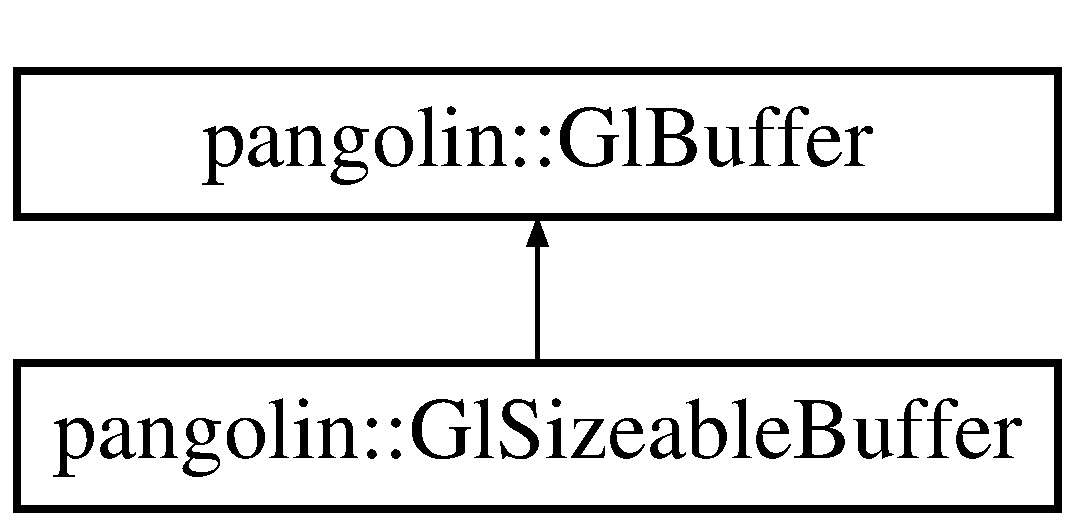
\includegraphics[height=2.000000cm]{classpangolin_1_1_gl_sizeable_buffer}
\end{center}
\end{figure}
\subsection*{Public Member Functions}
\begin{DoxyCompactItemize}
\item 
{\bfseries Gl\+Sizeable\+Buffer} (pangolin\+::\+Gl\+Buffer\+Type buffer\+\_\+type, G\+Luint initial\+\_\+num\+\_\+elements, G\+Lenum datatype, G\+Luint count\+\_\+per\+\_\+element, G\+Lenum gluse=G\+L\+\_\+\+D\+Y\+N\+A\+M\+I\+C\+\_\+\+D\+R\+AW)\hypertarget{classpangolin_1_1_gl_sizeable_buffer_ae85fb730a37da1481f389aa5116d5dd1}{}\label{classpangolin_1_1_gl_sizeable_buffer_ae85fb730a37da1481f389aa5116d5dd1}

\item 
void {\bfseries Clear} ()\hypertarget{classpangolin_1_1_gl_sizeable_buffer_a9ec9de9659f16f11c204635599f1fea5}{}\label{classpangolin_1_1_gl_sizeable_buffer_a9ec9de9659f16f11c204635599f1fea5}

\item 
size\+\_\+t {\bfseries start} () const \hypertarget{classpangolin_1_1_gl_sizeable_buffer_a4c4493fa7e7f7c53f9f91ffc17887c65}{}\label{classpangolin_1_1_gl_sizeable_buffer_a4c4493fa7e7f7c53f9f91ffc17887c65}

\item 
size\+\_\+t {\bfseries size} () const \hypertarget{classpangolin_1_1_gl_sizeable_buffer_aaa59deeffe8d5204673986ceeea069c6}{}\label{classpangolin_1_1_gl_sizeable_buffer_aaa59deeffe8d5204673986ceeea069c6}

\end{DoxyCompactItemize}
\subsection*{Protected Member Functions}
\begin{DoxyCompactItemize}
\item 
void {\bfseries Check\+Resize} (size\+\_\+t num\+\_\+verts)\hypertarget{classpangolin_1_1_gl_sizeable_buffer_af67d5857f7abe03821d179e950e42c2e}{}\label{classpangolin_1_1_gl_sizeable_buffer_af67d5857f7abe03821d179e950e42c2e}

\item 
size\+\_\+t {\bfseries Next\+Size} (size\+\_\+t min\+\_\+size) const \hypertarget{classpangolin_1_1_gl_sizeable_buffer_ae2292e7462a51d6ba70ba2853dc6a03f}{}\label{classpangolin_1_1_gl_sizeable_buffer_ae2292e7462a51d6ba70ba2853dc6a03f}

\end{DoxyCompactItemize}
\subsection*{Protected Attributes}
\begin{DoxyCompactItemize}
\item 
size\+\_\+t {\bfseries m\+\_\+num\+\_\+verts}\hypertarget{classpangolin_1_1_gl_sizeable_buffer_ac91f98b629308b87ddad90f1ad471406}{}\label{classpangolin_1_1_gl_sizeable_buffer_ac91f98b629308b87ddad90f1ad471406}

\end{DoxyCompactItemize}
\subsection*{Additional Inherited Members}


The documentation for this class was generated from the following file\+:\begin{DoxyCompactItemize}
\item 
/home/gapo/meng/deps/pangolin/include/pangolin/gl/gl.\+h\end{DoxyCompactItemize}

\hypertarget{classpangolin_1_1_gl_sl_program}{}\section{pangolin\+:\+:Gl\+Sl\+Program Class Reference}
\label{classpangolin_1_1_gl_sl_program}\index{pangolin\+::\+Gl\+Sl\+Program@{pangolin\+::\+Gl\+Sl\+Program}}
\subsection*{Public Member Functions}
\begin{DoxyCompactItemize}
\item 
bool {\bfseries Add\+Shader} (Gl\+Sl\+Shader\+Type shader\+\_\+type, const std\+::string \&source\+\_\+code, const std\+::map$<$ std\+::string, std\+::string $>$ \&program\+\_\+defines=std\+::map$<$ std\+::string, std\+::string $>$(), const std\+::vector$<$ std\+::string $>$ \&search\+\_\+path=std\+::vector$<$ std\+::string $>$())\hypertarget{classpangolin_1_1_gl_sl_program_a6880948ce17871643d9d7f1fea79e40f}{}\label{classpangolin_1_1_gl_sl_program_a6880948ce17871643d9d7f1fea79e40f}

\item 
bool {\bfseries Add\+Shader\+From\+File} (Gl\+Sl\+Shader\+Type shader\+\_\+type, const std\+::string \&filename, const std\+::map$<$ std\+::string, std\+::string $>$ \&program\+\_\+defines=std\+::map$<$ std\+::string, std\+::string $>$(), const std\+::vector$<$ std\+::string $>$ \&search\+\_\+path=std\+::vector$<$ std\+::string $>$())\hypertarget{classpangolin_1_1_gl_sl_program_afcf996e6d0de9b3a153de63e6d36ccdd}{}\label{classpangolin_1_1_gl_sl_program_afcf996e6d0de9b3a153de63e6d36ccdd}

\item 
bool {\bfseries Link} ()\hypertarget{classpangolin_1_1_gl_sl_program_a335888bedc6c9efd37b6c4313a80febc}{}\label{classpangolin_1_1_gl_sl_program_a335888bedc6c9efd37b6c4313a80febc}

\item 
G\+Lint {\bfseries Get\+Attribute\+Handle} (const std\+::string \&name)\hypertarget{classpangolin_1_1_gl_sl_program_a0445181368ce89c014e95a15bfd1b905}{}\label{classpangolin_1_1_gl_sl_program_a0445181368ce89c014e95a15bfd1b905}

\item 
G\+Lint {\bfseries Get\+Uniform\+Handle} (const std\+::string \&name)\hypertarget{classpangolin_1_1_gl_sl_program_a84634c0ec52ade204eb77f96f73f0266}{}\label{classpangolin_1_1_gl_sl_program_a84634c0ec52ade204eb77f96f73f0266}

\item 
void {\bfseries Set\+Uniform} (const std\+::string \&name, int x)\hypertarget{classpangolin_1_1_gl_sl_program_a5731be2af6fa53c17cfb35088b95a601}{}\label{classpangolin_1_1_gl_sl_program_a5731be2af6fa53c17cfb35088b95a601}

\item 
void {\bfseries Set\+Uniform} (const std\+::string \&name, int x1, int x2)\hypertarget{classpangolin_1_1_gl_sl_program_a3ca25f615d97242871d658bb6a1e4992}{}\label{classpangolin_1_1_gl_sl_program_a3ca25f615d97242871d658bb6a1e4992}

\item 
void {\bfseries Set\+Uniform} (const std\+::string \&name, int x1, int x2, int x3)\hypertarget{classpangolin_1_1_gl_sl_program_a63d941f091d09c131ed38d93c1349a72}{}\label{classpangolin_1_1_gl_sl_program_a63d941f091d09c131ed38d93c1349a72}

\item 
void {\bfseries Set\+Uniform} (const std\+::string \&name, int x1, int x2, int x3, int x4)\hypertarget{classpangolin_1_1_gl_sl_program_acac7526f33948068f3e2fe3cd57abacc}{}\label{classpangolin_1_1_gl_sl_program_acac7526f33948068f3e2fe3cd57abacc}

\item 
void {\bfseries Set\+Uniform} (const std\+::string \&name, float f)\hypertarget{classpangolin_1_1_gl_sl_program_a5db8cb062b0e0590c2ac5c20e2f7d7f1}{}\label{classpangolin_1_1_gl_sl_program_a5db8cb062b0e0590c2ac5c20e2f7d7f1}

\item 
void {\bfseries Set\+Uniform} (const std\+::string \&name, float f1, float f2)\hypertarget{classpangolin_1_1_gl_sl_program_a7ec9ea99220ddb382a04d461aa15ab28}{}\label{classpangolin_1_1_gl_sl_program_a7ec9ea99220ddb382a04d461aa15ab28}

\item 
void {\bfseries Set\+Uniform} (const std\+::string \&name, float f1, float f2, float f3)\hypertarget{classpangolin_1_1_gl_sl_program_ae3515f491cec31186996ee0d96c133f8}{}\label{classpangolin_1_1_gl_sl_program_ae3515f491cec31186996ee0d96c133f8}

\item 
void {\bfseries Set\+Uniform} (const std\+::string \&name, float f1, float f2, float f3, float f4)\hypertarget{classpangolin_1_1_gl_sl_program_a7b61e3c3986d934af45dca4b195aaca7}{}\label{classpangolin_1_1_gl_sl_program_a7b61e3c3986d934af45dca4b195aaca7}

\item 
void {\bfseries Set\+Uniform} (const std\+::string \&name, \hyperlink{structpangolin_1_1_colour}{Colour} c)\hypertarget{classpangolin_1_1_gl_sl_program_a77ede6406251fccc92ec635434a3b4ad}{}\label{classpangolin_1_1_gl_sl_program_a77ede6406251fccc92ec635434a3b4ad}

\item 
void {\bfseries Set\+Uniform} (const std\+::string \&name, const \hyperlink{structpangolin_1_1_open_gl_matrix}{Open\+Gl\+Matrix} \&m)\hypertarget{classpangolin_1_1_gl_sl_program_a5bca14ef8436d5db56e895632b6527ae}{}\label{classpangolin_1_1_gl_sl_program_a5bca14ef8436d5db56e895632b6527ae}

\item 
void {\bfseries Bind} ()\hypertarget{classpangolin_1_1_gl_sl_program_ad279f3dc5429b3da7d7dc0e516dcce0e}{}\label{classpangolin_1_1_gl_sl_program_ad279f3dc5429b3da7d7dc0e516dcce0e}

\item 
void {\bfseries Save\+Bind} ()\hypertarget{classpangolin_1_1_gl_sl_program_a45242b8df838a436d103504e16efbc81}{}\label{classpangolin_1_1_gl_sl_program_a45242b8df838a436d103504e16efbc81}

\item 
void {\bfseries Unbind} ()\hypertarget{classpangolin_1_1_gl_sl_program_a1e29f0a97f40b680395776414a477370}{}\label{classpangolin_1_1_gl_sl_program_a1e29f0a97f40b680395776414a477370}

\item 
void {\bfseries Bind\+Pangolin\+Default\+Attrib\+Locations\+And\+Link} ()\hypertarget{classpangolin_1_1_gl_sl_program_a6e48637494710a102122e0532abba2dd}{}\label{classpangolin_1_1_gl_sl_program_a6e48637494710a102122e0532abba2dd}

\end{DoxyCompactItemize}
\subsection*{Protected Member Functions}
\begin{DoxyCompactItemize}
\item 
std\+::string {\bfseries Parse\+Include\+Filename} (const std\+::string \&location)\hypertarget{classpangolin_1_1_gl_sl_program_ab3ddbf504d2c3f9027e11853f22928e1}{}\label{classpangolin_1_1_gl_sl_program_ab3ddbf504d2c3f9027e11853f22928e1}

\item 
std\+::string {\bfseries Search\+Include\+Path} (const std\+::string \&filename, const std\+::vector$<$ std\+::string $>$ \&search\+\_\+path, const std\+::string \&current\+\_\+path)\hypertarget{classpangolin_1_1_gl_sl_program_af8d35348ed13a2bcae13f489b1c957ba}{}\label{classpangolin_1_1_gl_sl_program_af8d35348ed13a2bcae13f489b1c957ba}

\item 
bool {\bfseries Add\+Preprocessed\+Shader} (Gl\+Sl\+Shader\+Type shader\+\_\+type, const std\+::string \&source\+\_\+code, const std\+::string \&name\+\_\+for\+\_\+errors)\hypertarget{classpangolin_1_1_gl_sl_program_adedca316d4367dfa2ab6c11ff6ca82cb}{}\label{classpangolin_1_1_gl_sl_program_adedca316d4367dfa2ab6c11ff6ca82cb}

\item 
void {\bfseries Parse\+G\+L\+SL} (std\+::istream \&input, std\+::ostream \&output, const std\+::map$<$ std\+::string, std\+::string $>$ \&program\+\_\+defines, const std\+::vector$<$ std\+::string $>$ \&search\+\_\+path, const std\+::string \&current\+\_\+path)\hypertarget{classpangolin_1_1_gl_sl_program_a6e2ace720497d9dc3d8bda29d0d2d9b6}{}\label{classpangolin_1_1_gl_sl_program_a6e2ace720497d9dc3d8bda29d0d2d9b6}

\end{DoxyCompactItemize}
\subsection*{Protected Attributes}
\begin{DoxyCompactItemize}
\item 
bool {\bfseries linked}\hypertarget{classpangolin_1_1_gl_sl_program_a451702d087219a5e434b80d935d25ad8}{}\label{classpangolin_1_1_gl_sl_program_a451702d087219a5e434b80d935d25ad8}

\item 
std\+::vector$<$ G\+Lhandle\+A\+RB $>$ {\bfseries shaders}\hypertarget{classpangolin_1_1_gl_sl_program_ad273d9dc9b3c1262d225ad82530bea6a}{}\label{classpangolin_1_1_gl_sl_program_ad273d9dc9b3c1262d225ad82530bea6a}

\item 
G\+Lenum {\bfseries prog}\hypertarget{classpangolin_1_1_gl_sl_program_a16644db3f31e33995eac41949c4344d8}{}\label{classpangolin_1_1_gl_sl_program_a16644db3f31e33995eac41949c4344d8}

\item 
G\+Lint {\bfseries prev\+\_\+prog}\hypertarget{classpangolin_1_1_gl_sl_program_aa4e51f100762bfd3599843ccdebc2714}{}\label{classpangolin_1_1_gl_sl_program_aa4e51f100762bfd3599843ccdebc2714}

\end{DoxyCompactItemize}


The documentation for this class was generated from the following file\+:\begin{DoxyCompactItemize}
\item 
/home/gapo/meng/deps/pangolin/include/pangolin/gl/glsl.\+h\end{DoxyCompactItemize}

\hypertarget{classpangolin_1_1_gl_sl_utilities}{}\section{pangolin\+:\+:Gl\+Sl\+Utilities Class Reference}
\label{classpangolin_1_1_gl_sl_utilities}\index{pangolin\+::\+Gl\+Sl\+Utilities@{pangolin\+::\+Gl\+Sl\+Utilities}}
\subsection*{Static Public Member Functions}
\begin{DoxyCompactItemize}
\item 
static \hyperlink{classpangolin_1_1_gl_sl_program}{Gl\+Sl\+Program} \& {\bfseries Offset\+And\+Scale} (float offset, float scale)\hypertarget{classpangolin_1_1_gl_sl_utilities_a356bb5a64cdf95e7188a5e29b69b5701}{}\label{classpangolin_1_1_gl_sl_utilities_a356bb5a64cdf95e7188a5e29b69b5701}

\item 
static \hyperlink{classpangolin_1_1_gl_sl_program}{Gl\+Sl\+Program} \& {\bfseries Scale} (float scale, float bias=0.\+0f)\hypertarget{classpangolin_1_1_gl_sl_utilities_a7637bc12aec59edd4fdfae4dc7c99164}{}\label{classpangolin_1_1_gl_sl_utilities_a7637bc12aec59edd4fdfae4dc7c99164}

\item 
static void {\bfseries Use\+None} ()\hypertarget{classpangolin_1_1_gl_sl_utilities_aad4e8128902561b1a3ab48a1fc8a6412}{}\label{classpangolin_1_1_gl_sl_utilities_aad4e8128902561b1a3ab48a1fc8a6412}

\end{DoxyCompactItemize}
\subsection*{Static Protected Member Functions}
\begin{DoxyCompactItemize}
\item 
static \hyperlink{classpangolin_1_1_gl_sl_utilities}{Gl\+Sl\+Utilities} \& {\bfseries Instance} ()\hypertarget{classpangolin_1_1_gl_sl_utilities_af4c5f3055d06baec8964cca3fcffd2e7}{}\label{classpangolin_1_1_gl_sl_utilities_af4c5f3055d06baec8964cca3fcffd2e7}

\end{DoxyCompactItemize}
\subsection*{Protected Attributes}
\begin{DoxyCompactItemize}
\item 
\hyperlink{classpangolin_1_1_gl_sl_program}{Gl\+Sl\+Program} {\bfseries prog\+\_\+scale}\hypertarget{classpangolin_1_1_gl_sl_utilities_a1d740b28056c07082b64c5d6a6c07bc0}{}\label{classpangolin_1_1_gl_sl_utilities_a1d740b28056c07082b64c5d6a6c07bc0}

\item 
\hyperlink{classpangolin_1_1_gl_sl_program}{Gl\+Sl\+Program} {\bfseries prog\+\_\+offsetscale}\hypertarget{classpangolin_1_1_gl_sl_utilities_a537c701c772160cbfb2c1e642b5af395}{}\label{classpangolin_1_1_gl_sl_utilities_a537c701c772160cbfb2c1e642b5af395}

\end{DoxyCompactItemize}


The documentation for this class was generated from the following file\+:\begin{DoxyCompactItemize}
\item 
/home/gapo/meng/deps/pangolin/include/pangolin/gl/glsl.\+h\end{DoxyCompactItemize}

\hypertarget{classpangolin_1_1_gl_state}{}\section{pangolin\+:\+:Gl\+State Class Reference}
\label{classpangolin_1_1_gl_state}\index{pangolin\+::\+Gl\+State@{pangolin\+::\+Gl\+State}}
\subsection*{Public Member Functions}
\begin{DoxyCompactItemize}
\item 
void {\bfseries gl\+Enable} (G\+Lenum cap)\hypertarget{classpangolin_1_1_gl_state_acbab4ce959bb3a21e89833a3395cb767}{}\label{classpangolin_1_1_gl_state_acbab4ce959bb3a21e89833a3395cb767}

\item 
void {\bfseries gl\+Disable} (G\+Lenum cap)\hypertarget{classpangolin_1_1_gl_state_a27249f592db3adc84725d2fa97906ffc}{}\label{classpangolin_1_1_gl_state_a27249f592db3adc84725d2fa97906ffc}

\item 
void {\bfseries gl\+Depth\+Mask} (G\+Lboolean flag)\hypertarget{classpangolin_1_1_gl_state_a546766c0bc813c5ee25cc1644170c583}{}\label{classpangolin_1_1_gl_state_a546766c0bc813c5ee25cc1644170c583}

\item 
void {\bfseries gl\+Shade\+Model} (G\+Lint mode)\hypertarget{classpangolin_1_1_gl_state_a83bc993d1685aa6717432a27d5527ea4}{}\label{classpangolin_1_1_gl_state_a83bc993d1685aa6717432a27d5527ea4}

\item 
void {\bfseries gl\+Cull\+Face} (G\+Lenum mode)\hypertarget{classpangolin_1_1_gl_state_a1a14835dd0236431983f1e84492eac72}{}\label{classpangolin_1_1_gl_state_a1a14835dd0236431983f1e84492eac72}

\item 
void {\bfseries gl\+Point\+Size} (G\+Lfloat size)\hypertarget{classpangolin_1_1_gl_state_ad89ff5be459d839e9876ec473c81791a}{}\label{classpangolin_1_1_gl_state_ad89ff5be459d839e9876ec473c81791a}

\item 
void {\bfseries gl\+Line\+Width} (G\+Lfloat width)\hypertarget{classpangolin_1_1_gl_state_ae7b13f1387b3c571b198d19d6779c16b}{}\label{classpangolin_1_1_gl_state_ae7b13f1387b3c571b198d19d6779c16b}

\item 
void {\bfseries gl\+Color\+Mask} (G\+Lboolean red, G\+Lboolean green, G\+Lboolean blue, G\+Lboolean alpha)\hypertarget{classpangolin_1_1_gl_state_adfc2b30467d7c506737406de44aa2ca5}{}\label{classpangolin_1_1_gl_state_adfc2b30467d7c506737406de44aa2ca5}

\item 
void {\bfseries gl\+Viewport} (G\+Lint x, G\+Lint y, G\+Lsizei width, G\+Lsizei height)\hypertarget{classpangolin_1_1_gl_state_a1445f136d0fc99dd011ff0680c2cabcf}{}\label{classpangolin_1_1_gl_state_a1445f136d0fc99dd011ff0680c2cabcf}

\end{DoxyCompactItemize}
\subsection*{Static Public Member Functions}
\begin{DoxyCompactItemize}
\item 
static G\+Lboolean {\bfseries Is\+Enabled} (G\+Lenum cap)\hypertarget{classpangolin_1_1_gl_state_a97db77ba073cac7084bdd457a1572a32}{}\label{classpangolin_1_1_gl_state_a97db77ba073cac7084bdd457a1572a32}

\end{DoxyCompactItemize}
\subsection*{Public Attributes}
\begin{DoxyCompactItemize}
\item 
bool {\bfseries m\+\_\+\+Depth\+Mask\+Called}\hypertarget{classpangolin_1_1_gl_state_afedb7765bdeea3dfa74993caea9d0fc6}{}\label{classpangolin_1_1_gl_state_afedb7765bdeea3dfa74993caea9d0fc6}

\item 
G\+Lboolean {\bfseries m\+\_\+\+Original\+Depth\+Mask}\hypertarget{classpangolin_1_1_gl_state_ad273b32587d3cbf3fbaeaffdaf058d3a}{}\label{classpangolin_1_1_gl_state_ad273b32587d3cbf3fbaeaffdaf058d3a}

\item 
bool {\bfseries m\+\_\+\+Shade\+Model\+Called}\hypertarget{classpangolin_1_1_gl_state_ae3d9e06c8accf4dd47f446b853660fb2}{}\label{classpangolin_1_1_gl_state_ae3d9e06c8accf4dd47f446b853660fb2}

\item 
G\+Lint {\bfseries m\+\_\+\+Original\+Shade\+Model}\hypertarget{classpangolin_1_1_gl_state_ad81319f85b2e427d444756ec5602629b}{}\label{classpangolin_1_1_gl_state_ad81319f85b2e427d444756ec5602629b}

\item 
bool {\bfseries m\+\_\+\+Cull\+Face\+Called}\hypertarget{classpangolin_1_1_gl_state_a9d1a2ff2b0a74c2c2bc0718f8f6a5822}{}\label{classpangolin_1_1_gl_state_a9d1a2ff2b0a74c2c2bc0718f8f6a5822}

\item 
G\+Lint {\bfseries m\+\_\+\+Original\+Cull\+Face}\hypertarget{classpangolin_1_1_gl_state_af6e06e270f71d5e6a19b1e08575ec793}{}\label{classpangolin_1_1_gl_state_af6e06e270f71d5e6a19b1e08575ec793}

\item 
bool {\bfseries m\+\_\+\+Point\+Size\+Called}\hypertarget{classpangolin_1_1_gl_state_a2c27e8f5699e8e54a54f7c3e73a956f1}{}\label{classpangolin_1_1_gl_state_a2c27e8f5699e8e54a54f7c3e73a956f1}

\item 
G\+Lfloat {\bfseries m\+\_\+\+Original\+Point\+Size}\hypertarget{classpangolin_1_1_gl_state_a10ef0c06828799998dba1e6e2811760b}{}\label{classpangolin_1_1_gl_state_a10ef0c06828799998dba1e6e2811760b}

\item 
bool {\bfseries m\+\_\+\+Line\+Width\+Called}\hypertarget{classpangolin_1_1_gl_state_a05154114643249c161ba4414028f1172}{}\label{classpangolin_1_1_gl_state_a05154114643249c161ba4414028f1172}

\item 
G\+Lfloat {\bfseries m\+\_\+\+Original\+Line\+Width}\hypertarget{classpangolin_1_1_gl_state_ae76ecedcea967fb5e7d7459675e530cf}{}\label{classpangolin_1_1_gl_state_ae76ecedcea967fb5e7d7459675e530cf}

\item 
bool {\bfseries m\+\_\+\+Color\+Mask\+Called}\hypertarget{classpangolin_1_1_gl_state_a113bff8417500bb8d9794e0dd5cb06be}{}\label{classpangolin_1_1_gl_state_a113bff8417500bb8d9794e0dd5cb06be}

\item 
G\+Lboolean {\bfseries m\+\_\+\+Original\+Color\+Mask} \mbox{[}4\mbox{]}\hypertarget{classpangolin_1_1_gl_state_ae509573e080448c1577e816416bb8dba}{}\label{classpangolin_1_1_gl_state_ae509573e080448c1577e816416bb8dba}

\item 
bool {\bfseries m\+\_\+\+Viewport\+Called}\hypertarget{classpangolin_1_1_gl_state_acca68f34837cc0a220433f5eba2c72ba}{}\label{classpangolin_1_1_gl_state_acca68f34837cc0a220433f5eba2c72ba}

\item 
G\+Lint {\bfseries m\+\_\+\+Original\+Viewport} \mbox{[}4\mbox{]}\hypertarget{classpangolin_1_1_gl_state_a3ff4eec68e8a21ce1b74ecad53130970}{}\label{classpangolin_1_1_gl_state_a3ff4eec68e8a21ce1b74ecad53130970}

\item 
std\+::stack$<$ Capability\+State $>$ {\bfseries m\+\_\+history}\hypertarget{classpangolin_1_1_gl_state_a5bc01b0a47792e842e83c674c71293ff}{}\label{classpangolin_1_1_gl_state_a5bc01b0a47792e842e83c674c71293ff}

\end{DoxyCompactItemize}


The documentation for this class was generated from the following file\+:\begin{DoxyCompactItemize}
\item 
/home/gapo/meng/deps/pangolin/include/pangolin/gl/glstate.\+h\end{DoxyCompactItemize}

\hypertarget{classpangolin_1_1_gl_text}{}\section{pangolin\+:\+:Gl\+Text Class Reference}
\label{classpangolin_1_1_gl_text}\index{pangolin\+::\+Gl\+Text@{pangolin\+::\+Gl\+Text}}
\subsection*{Public Member Functions}
\begin{DoxyCompactItemize}
\item 
{\bfseries Gl\+Text} (const \hyperlink{classpangolin_1_1_gl_text}{Gl\+Text} \&txt)\hypertarget{classpangolin_1_1_gl_text_a7da26b24cb14123c130e11e5bb3e96a9}{}\label{classpangolin_1_1_gl_text_a7da26b24cb14123c130e11e5bb3e96a9}

\item 
{\bfseries Gl\+Text} (const \hyperlink{classpangolin_1_1_gl_texture}{Gl\+Texture} \&font\+\_\+tex)\hypertarget{classpangolin_1_1_gl_text_a4a719f2d9cdb7ab78f3d55b59b87a973}{}\label{classpangolin_1_1_gl_text_a4a719f2d9cdb7ab78f3d55b59b87a973}

\item 
void {\bfseries Add\+Space} (G\+Lfloat s)\hypertarget{classpangolin_1_1_gl_text_a585e5c17349f04fbc35acbcc6ec4f97b}{}\label{classpangolin_1_1_gl_text_a585e5c17349f04fbc35acbcc6ec4f97b}

\item 
void {\bfseries Add} (unsigned char c, const \hyperlink{classpangolin_1_1_gl_char}{Gl\+Char} \&glc)\hypertarget{classpangolin_1_1_gl_text_a8568901ba44b67c2a524390faa185101}{}\label{classpangolin_1_1_gl_text_a8568901ba44b67c2a524390faa185101}

\item 
void {\bfseries Clear} ()\hypertarget{classpangolin_1_1_gl_text_a63db7d32f57a88fc2c2acaaa47b56e0f}{}\label{classpangolin_1_1_gl_text_a63db7d32f57a88fc2c2acaaa47b56e0f}

\item 
void {\bfseries Draw} () const \hypertarget{classpangolin_1_1_gl_text_a3de9dc9caf9196a4b76674a70b585ebf}{}\label{classpangolin_1_1_gl_text_a3de9dc9caf9196a4b76674a70b585ebf}

\item 
void {\bfseries Draw\+Gl\+Sl} () const \hypertarget{classpangolin_1_1_gl_text_ad0d8fe41c8edbe93032d38e3f73a59c6}{}\label{classpangolin_1_1_gl_text_ad0d8fe41c8edbe93032d38e3f73a59c6}

\item 
const std\+::string \& {\bfseries Text} () const \hypertarget{classpangolin_1_1_gl_text_afa0399233f7cf0840b16853291b817a1}{}\label{classpangolin_1_1_gl_text_afa0399233f7cf0840b16853291b817a1}

\item 
G\+Lfloat {\bfseries Width} () const \hypertarget{classpangolin_1_1_gl_text_a0b30ad96ac8a8ec1eea988590bfdc4e0}{}\label{classpangolin_1_1_gl_text_a0b30ad96ac8a8ec1eea988590bfdc4e0}

\item 
G\+Lfloat {\bfseries Height} () const \hypertarget{classpangolin_1_1_gl_text_ac7caf155d21a0ebfefd4aa88f9a31530}{}\label{classpangolin_1_1_gl_text_ac7caf155d21a0ebfefd4aa88f9a31530}

\item 
G\+Lfloat {\bfseries Full\+Height} () const \hypertarget{classpangolin_1_1_gl_text_a1e0e66fb85d375e923553d5e5f46b8ec}{}\label{classpangolin_1_1_gl_text_a1e0e66fb85d375e923553d5e5f46b8ec}

\end{DoxyCompactItemize}
\subsection*{Public Attributes}
\begin{DoxyCompactItemize}
\item 
const \hyperlink{classpangolin_1_1_gl_texture}{Gl\+Texture} $\ast$ {\bfseries tex}\hypertarget{classpangolin_1_1_gl_text_a0f67ea2fa7e61ac75cdf7425b69811c0}{}\label{classpangolin_1_1_gl_text_a0f67ea2fa7e61ac75cdf7425b69811c0}

\item 
std\+::string {\bfseries str}\hypertarget{classpangolin_1_1_gl_text_a188146b599b31f8d27b7d7eada5a5d98}{}\label{classpangolin_1_1_gl_text_a188146b599b31f8d27b7d7eada5a5d98}

\item 
G\+Lfloat {\bfseries width}\hypertarget{classpangolin_1_1_gl_text_acdd19374b030621fee47ced19fd60c7e}{}\label{classpangolin_1_1_gl_text_acdd19374b030621fee47ced19fd60c7e}

\item 
G\+Lfloat {\bfseries ymin}\hypertarget{classpangolin_1_1_gl_text_a37d65bd516b9ebc1f7b2f63309741a3c}{}\label{classpangolin_1_1_gl_text_a37d65bd516b9ebc1f7b2f63309741a3c}

\item 
G\+Lfloat {\bfseries ymax}\hypertarget{classpangolin_1_1_gl_text_a1efac36dcdb3ee29b501195fa6723800}{}\label{classpangolin_1_1_gl_text_a1efac36dcdb3ee29b501195fa6723800}

\item 
std\+::vector$<$ \hyperlink{structpangolin_1_1_x_y_u_v}{X\+Y\+UV} $>$ {\bfseries vs}\hypertarget{classpangolin_1_1_gl_text_a1f512a84a6d2f4146d19a7578dfebfa2}{}\label{classpangolin_1_1_gl_text_a1f512a84a6d2f4146d19a7578dfebfa2}

\end{DoxyCompactItemize}


The documentation for this class was generated from the following file\+:\begin{DoxyCompactItemize}
\item 
/home/gapo/meng/deps/pangolin/include/pangolin/gl/gltext.\+h\end{DoxyCompactItemize}

\hypertarget{classpangolin_1_1_gl_texture}{}\section{pangolin\+:\+:Gl\+Texture Class Reference}
\label{classpangolin_1_1_gl_texture}\index{pangolin\+::\+Gl\+Texture@{pangolin\+::\+Gl\+Texture}}
Inheritance diagram for pangolin\+:\+:Gl\+Texture\+:\begin{figure}[H]
\begin{center}
\leavevmode
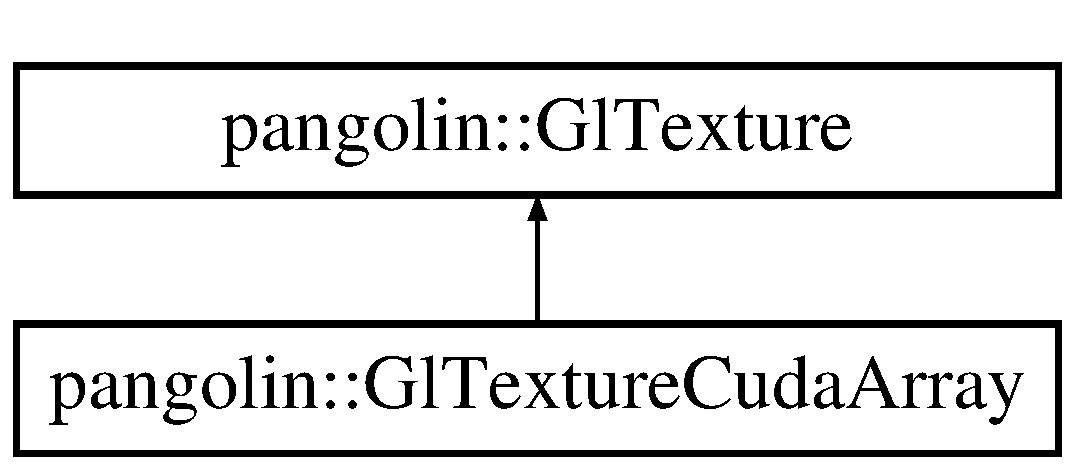
\includegraphics[height=2.000000cm]{classpangolin_1_1_gl_texture}
\end{center}
\end{figure}
\subsection*{Public Member Functions}
\begin{DoxyCompactItemize}
\item 
\hyperlink{classpangolin_1_1_gl_texture_addf883bdafe29c5135ef0990fc7ef3cd}{Gl\+Texture} (G\+Lint width, G\+Lint height, G\+Lint internal\+\_\+format=G\+L\+\_\+\+R\+G\+BA, bool sampling\+\_\+linear=true, int border=0, G\+Lenum glformat=G\+L\+\_\+\+R\+G\+BA, G\+Lenum gltype=G\+L\+\_\+\+U\+N\+S\+I\+G\+N\+E\+D\+\_\+\+B\+Y\+TE, G\+Lvoid $\ast$data=N\+U\+LL)\hypertarget{classpangolin_1_1_gl_texture_addf883bdafe29c5135ef0990fc7ef3cd}{}\label{classpangolin_1_1_gl_texture_addf883bdafe29c5135ef0990fc7ef3cd}

\begin{DoxyCompactList}\small\item\em internal\+\_\+format normally one of G\+L\+\_\+\+R\+G\+B\+A8, G\+L\+\_\+\+L\+U\+M\+I\+N\+A\+N\+C\+E8, G\+L\+\_\+\+I\+N\+T\+E\+N\+S\+I\+T\+Y16 \end{DoxyCompactList}\item 
\hyperlink{classpangolin_1_1_gl_texture_a009961fdb69716e2f00ead3a9aee0e15}{Gl\+Texture} ()\hypertarget{classpangolin_1_1_gl_texture_a009961fdb69716e2f00ead3a9aee0e15}{}\label{classpangolin_1_1_gl_texture_a009961fdb69716e2f00ead3a9aee0e15}

\begin{DoxyCompactList}\small\item\em Default constructor represents \textquotesingle{}no texture\textquotesingle{}. \end{DoxyCompactList}\item 
bool {\bfseries Is\+Valid} () const \hypertarget{classpangolin_1_1_gl_texture_ad860c1ffa1fc1a699aeb0c2e49efbe71}{}\label{classpangolin_1_1_gl_texture_ad860c1ffa1fc1a699aeb0c2e49efbe71}

\item 
void \hyperlink{classpangolin_1_1_gl_texture_aa2d520d9d1f2d68166bcdc6ce7b7eb33}{Delete} ()\hypertarget{classpangolin_1_1_gl_texture_aa2d520d9d1f2d68166bcdc6ce7b7eb33}{}\label{classpangolin_1_1_gl_texture_aa2d520d9d1f2d68166bcdc6ce7b7eb33}

\begin{DoxyCompactList}\small\item\em Delete Open\+GL resources and fall back to representing \textquotesingle{}no texture\textquotesingle{}. \end{DoxyCompactList}\item 
void \hyperlink{classpangolin_1_1_gl_texture_ac130d85fde9b0936b5b57dd174fde6df}{Reinitialise} (G\+Lint width, G\+Lint height, G\+Lint internal\+\_\+format=G\+L\+\_\+\+R\+G\+BA, bool sampling\+\_\+linear=true, int border=0, G\+Lenum glformat=G\+L\+\_\+\+R\+G\+BA, G\+Lenum gltype=G\+L\+\_\+\+U\+N\+S\+I\+G\+N\+E\+D\+\_\+\+B\+Y\+TE, G\+Lvoid $\ast$data=N\+U\+LL)\hypertarget{classpangolin_1_1_gl_texture_ac130d85fde9b0936b5b57dd174fde6df}{}\label{classpangolin_1_1_gl_texture_ac130d85fde9b0936b5b57dd174fde6df}

\begin{DoxyCompactList}\small\item\em Reinitialise teture width / height / format. \end{DoxyCompactList}\item 
void {\bfseries Bind} () const \hypertarget{classpangolin_1_1_gl_texture_a7b6da38e7ca3222d08c0cac2ca98a218}{}\label{classpangolin_1_1_gl_texture_a7b6da38e7ca3222d08c0cac2ca98a218}

\item 
void {\bfseries Unbind} () const \hypertarget{classpangolin_1_1_gl_texture_ab37bc2e23047a1f6f9a571ad5fbfb476}{}\label{classpangolin_1_1_gl_texture_ab37bc2e23047a1f6f9a571ad5fbfb476}

\item 
void \hyperlink{classpangolin_1_1_gl_texture_a5d01b592367029975714da0062b8f6f9}{Upload} (const void $\ast$image, G\+Lenum data\+\_\+format=G\+L\+\_\+\+L\+U\+M\+I\+N\+A\+N\+CE, G\+Lenum data\+\_\+type=G\+L\+\_\+\+F\+L\+O\+AT)
\begin{DoxyCompactList}\small\item\em data\+\_\+layout normally one of G\+L\+\_\+\+L\+U\+M\+I\+N\+A\+N\+CE, G\+L\+\_\+\+R\+GB, ... \end{DoxyCompactList}\item 
void \hyperlink{classpangolin_1_1_gl_texture_ad78ac40f91fb27d65705608c35c972c0}{Upload} (const void $\ast$data, unsigned int tex\+\_\+x\+\_\+offset, unsigned int tex\+\_\+y\+\_\+offset, unsigned int data\+\_\+w, unsigned int data\+\_\+h, G\+Lenum data\+\_\+format, G\+Lenum data\+\_\+type)
\begin{DoxyCompactList}\small\item\em Upload data to texture, overwriting a sub-\/region of it. \end{DoxyCompactList}\item 
void {\bfseries Load} (const \hyperlink{structpangolin_1_1_typed_image}{Typed\+Image} \&image, bool sampling\+\_\+linear=true)\hypertarget{classpangolin_1_1_gl_texture_a0407f01869fd270aab991116162d936b}{}\label{classpangolin_1_1_gl_texture_a0407f01869fd270aab991116162d936b}

\item 
void {\bfseries Load\+From\+File} (const std\+::string \&filename, bool sampling\+\_\+linear=true)\hypertarget{classpangolin_1_1_gl_texture_ab7601520d0133e540c192f1d1fa2fd93}{}\label{classpangolin_1_1_gl_texture_ab7601520d0133e540c192f1d1fa2fd93}

\item 
void {\bfseries Download} (void $\ast$image, G\+Lenum data\+\_\+layout=G\+L\+\_\+\+L\+U\+M\+I\+N\+A\+N\+CE, G\+Lenum data\+\_\+type=G\+L\+\_\+\+F\+L\+O\+AT) const \hypertarget{classpangolin_1_1_gl_texture_a062809c9c598692fafd039a5f64e9622}{}\label{classpangolin_1_1_gl_texture_a062809c9c598692fafd039a5f64e9622}

\item 
void {\bfseries Save} (const std\+::string \&filename, bool top\+\_\+line\+\_\+first=true)\hypertarget{classpangolin_1_1_gl_texture_ae8b002a221eefa9871e8a8233f34ddc1}{}\label{classpangolin_1_1_gl_texture_ae8b002a221eefa9871e8a8233f34ddc1}

\item 
void {\bfseries Set\+Linear} ()\hypertarget{classpangolin_1_1_gl_texture_aab0a12025f129a4bd4ce8e7fe732d727}{}\label{classpangolin_1_1_gl_texture_aab0a12025f129a4bd4ce8e7fe732d727}

\item 
void {\bfseries Set\+Nearest\+Neighbour} ()\hypertarget{classpangolin_1_1_gl_texture_aa30d98009f39b9e6946134505fa4b87d}{}\label{classpangolin_1_1_gl_texture_aa30d98009f39b9e6946134505fa4b87d}

\item 
void {\bfseries Render\+To\+Viewport} (const bool flip) const \hypertarget{classpangolin_1_1_gl_texture_a91a8d237faf8dc021dcd2190b1f57837}{}\label{classpangolin_1_1_gl_texture_a91a8d237faf8dc021dcd2190b1f57837}

\item 
void {\bfseries Render\+To\+Viewport} () const \hypertarget{classpangolin_1_1_gl_texture_a4ab143bc3dcbaa056ee674fb121751ea}{}\label{classpangolin_1_1_gl_texture_a4ab143bc3dcbaa056ee674fb121751ea}

\item 
void {\bfseries Render\+To\+Viewport} (\hyperlink{structpangolin_1_1_viewport}{Viewport} tex\+\_\+vp, bool flipx=false, bool flipy=false) const \hypertarget{classpangolin_1_1_gl_texture_a53afa64af3be9b786aa58ce737d20833}{}\label{classpangolin_1_1_gl_texture_a53afa64af3be9b786aa58ce737d20833}

\item 
void {\bfseries Render\+To\+Viewport\+FlipY} () const \hypertarget{classpangolin_1_1_gl_texture_a308da3c55bb8bb6dc36c780be9e6c718}{}\label{classpangolin_1_1_gl_texture_a308da3c55bb8bb6dc36c780be9e6c718}

\item 
void {\bfseries Render\+To\+Viewport\+Flip\+X\+FlipY} () const \hypertarget{classpangolin_1_1_gl_texture_ab4a06f047c643210ac058abbcc0b8481}{}\label{classpangolin_1_1_gl_texture_ab4a06f047c643210ac058abbcc0b8481}

\end{DoxyCompactItemize}
\subsection*{Public Attributes}
\begin{DoxyCompactItemize}
\item 
G\+Lint {\bfseries internal\+\_\+format}\hypertarget{classpangolin_1_1_gl_texture_a34e33d1aecc876d45f86a5cc7c6d496b}{}\label{classpangolin_1_1_gl_texture_a34e33d1aecc876d45f86a5cc7c6d496b}

\item 
G\+Luint {\bfseries tid}\hypertarget{classpangolin_1_1_gl_texture_a706705803a99c28f4b0280dc381074cc}{}\label{classpangolin_1_1_gl_texture_a706705803a99c28f4b0280dc381074cc}

\item 
G\+Lint {\bfseries width}\hypertarget{classpangolin_1_1_gl_texture_a7f659b562ca69b0aa3d23cf6bea5326b}{}\label{classpangolin_1_1_gl_texture_a7f659b562ca69b0aa3d23cf6bea5326b}

\item 
G\+Lint {\bfseries height}\hypertarget{classpangolin_1_1_gl_texture_aafdae9fa0e4b38d8446840598a37092b}{}\label{classpangolin_1_1_gl_texture_aafdae9fa0e4b38d8446840598a37092b}

\end{DoxyCompactItemize}


\subsection{Member Function Documentation}
\index{pangolin\+::\+Gl\+Texture@{pangolin\+::\+Gl\+Texture}!Upload@{Upload}}
\index{Upload@{Upload}!pangolin\+::\+Gl\+Texture@{pangolin\+::\+Gl\+Texture}}
\subsubsection[{\texorpdfstring{Upload(const void $\ast$image, G\+Lenum data\+\_\+format=\+G\+L\+\_\+\+L\+U\+M\+I\+N\+A\+N\+C\+E, G\+Lenum data\+\_\+type=\+G\+L\+\_\+\+F\+L\+O\+A\+T)}{Upload(const void *image, GLenum data_format=GL_LUMINANCE, GLenum data_type=GL_FLOAT)}}]{\setlength{\rightskip}{0pt plus 5cm}void pangolin\+::\+Gl\+Texture\+::\+Upload (
\begin{DoxyParamCaption}
\item[{const void $\ast$}]{image, }
\item[{G\+Lenum}]{data\+\_\+format = {\ttfamily GL\+\_\+LUMINANCE}, }
\item[{G\+Lenum}]{data\+\_\+type = {\ttfamily GL\+\_\+FLOAT}}
\end{DoxyParamCaption}
)}\hypertarget{classpangolin_1_1_gl_texture_a5d01b592367029975714da0062b8f6f9}{}\label{classpangolin_1_1_gl_texture_a5d01b592367029975714da0062b8f6f9}


data\+\_\+layout normally one of G\+L\+\_\+\+L\+U\+M\+I\+N\+A\+N\+CE, G\+L\+\_\+\+R\+GB, ... 

data\+\_\+type normally one of G\+L\+\_\+\+U\+N\+S\+I\+G\+N\+E\+D\+\_\+\+B\+Y\+TE, G\+L\+\_\+\+U\+N\+S\+I\+G\+N\+E\+D\+\_\+\+S\+H\+O\+RT, G\+L\+\_\+\+F\+L\+O\+AT \index{pangolin\+::\+Gl\+Texture@{pangolin\+::\+Gl\+Texture}!Upload@{Upload}}
\index{Upload@{Upload}!pangolin\+::\+Gl\+Texture@{pangolin\+::\+Gl\+Texture}}
\subsubsection[{\texorpdfstring{Upload(const void $\ast$data, unsigned int tex\+\_\+x\+\_\+offset, unsigned int tex\+\_\+y\+\_\+offset, unsigned int data\+\_\+w, unsigned int data\+\_\+h, G\+Lenum data\+\_\+format, G\+Lenum data\+\_\+type)}{Upload(const void *data, unsigned int tex_x_offset, unsigned int tex_y_offset, unsigned int data_w, unsigned int data_h, GLenum data_format, GLenum data_type)}}]{\setlength{\rightskip}{0pt plus 5cm}void pangolin\+::\+Gl\+Texture\+::\+Upload (
\begin{DoxyParamCaption}
\item[{const void $\ast$}]{data, }
\item[{unsigned int}]{tex\+\_\+x\+\_\+offset, }
\item[{unsigned int}]{tex\+\_\+y\+\_\+offset, }
\item[{unsigned int}]{data\+\_\+w, }
\item[{unsigned int}]{data\+\_\+h, }
\item[{G\+Lenum}]{data\+\_\+format, }
\item[{G\+Lenum}]{data\+\_\+type}
\end{DoxyParamCaption}
)}\hypertarget{classpangolin_1_1_gl_texture_ad78ac40f91fb27d65705608c35c972c0}{}\label{classpangolin_1_1_gl_texture_ad78ac40f91fb27d65705608c35c972c0}


Upload data to texture, overwriting a sub-\/region of it. 

data ptr contains packed data\+\_\+w x data\+\_\+h of pixel data. 

The documentation for this class was generated from the following file\+:\begin{DoxyCompactItemize}
\item 
/home/gapo/meng/deps/pangolin/include/pangolin/gl/gl.\+h\end{DoxyCompactItemize}

\hypertarget{structpangolin_1_1_gl_texture_cuda_array}{}\section{pangolin\+:\+:Gl\+Texture\+Cuda\+Array Struct Reference}
\label{structpangolin_1_1_gl_texture_cuda_array}\index{pangolin\+::\+Gl\+Texture\+Cuda\+Array@{pangolin\+::\+Gl\+Texture\+Cuda\+Array}}
Inheritance diagram for pangolin\+:\+:Gl\+Texture\+Cuda\+Array\+:\begin{figure}[H]
\begin{center}
\leavevmode
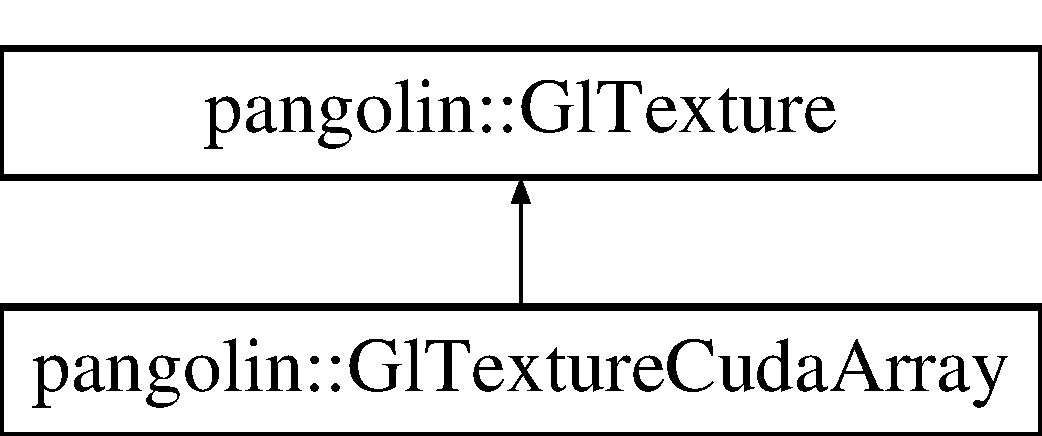
\includegraphics[height=2.000000cm]{structpangolin_1_1_gl_texture_cuda_array}
\end{center}
\end{figure}
\subsection*{Public Member Functions}
\begin{DoxyCompactItemize}
\item 
{\bfseries Gl\+Texture\+Cuda\+Array} (int width, int height, G\+Lint internal\+\_\+format, bool sampling\+\_\+linear=true)\hypertarget{structpangolin_1_1_gl_texture_cuda_array_aa33dc18a2f7491a01480ccd0ab19a407}{}\label{structpangolin_1_1_gl_texture_cuda_array_aa33dc18a2f7491a01480ccd0ab19a407}

\item 
void {\bfseries Reinitialise} (int width, int height, G\+Lint internal\+\_\+format, bool sampling\+\_\+linear=true)\hypertarget{structpangolin_1_1_gl_texture_cuda_array_ab83d262e62926c98256560d1ab317b64}{}\label{structpangolin_1_1_gl_texture_cuda_array_ab83d262e62926c98256560d1ab317b64}

\end{DoxyCompactItemize}
\subsection*{Public Attributes}
\begin{DoxyCompactItemize}
\item 
cuda\+Graphics\+Resource $\ast$ {\bfseries cuda\+\_\+res}\hypertarget{structpangolin_1_1_gl_texture_cuda_array_a9916894dec0e9041f113858b1518934d}{}\label{structpangolin_1_1_gl_texture_cuda_array_a9916894dec0e9041f113858b1518934d}

\end{DoxyCompactItemize}


The documentation for this struct was generated from the following file\+:\begin{DoxyCompactItemize}
\item 
/home/gapo/meng/deps/pangolin/include/pangolin/gl/glcuda.\+h\end{DoxyCompactItemize}

\hypertarget{structpangolin_1_1_guid}{}\section{pangolin\+:\+:Guid Struct Reference}
\label{structpangolin_1_1_guid}\index{pangolin\+::\+Guid@{pangolin\+::\+Guid}}
\subsection*{Public Member Functions}
\begin{DoxyCompactItemize}
\item 
{\bfseries Guid} (uint64\+\_\+t guid)\hypertarget{structpangolin_1_1_guid_a6246eeb3363204f7004042e1fc993eb9}{}\label{structpangolin_1_1_guid_a6246eeb3363204f7004042e1fc993eb9}

\end{DoxyCompactItemize}
\subsection*{Public Attributes}
\begin{DoxyCompactItemize}
\item 
uint64\+\_\+t {\bfseries guid}\hypertarget{structpangolin_1_1_guid_a34bd8df4841301fe8d1cf45ece292b0f}{}\label{structpangolin_1_1_guid_a34bd8df4841301fe8d1cf45ece292b0f}

\end{DoxyCompactItemize}


The documentation for this struct was generated from the following file\+:\begin{DoxyCompactItemize}
\item 
/home/gapo/meng/deps/pangolin/include/pangolin/video/drivers/firewire.\+h\end{DoxyCompactItemize}

\hypertarget{structpangolin_1_1_gui_var_changed_callback}{}\section{pangolin\+:\+:Gui\+Var\+Changed\+Callback Struct Reference}
\label{structpangolin_1_1_gui_var_changed_callback}\index{pangolin\+::\+Gui\+Var\+Changed\+Callback@{pangolin\+::\+Gui\+Var\+Changed\+Callback}}
\subsection*{Public Member Functions}
\begin{DoxyCompactItemize}
\item 
{\bfseries Gui\+Var\+Changed\+Callback} (const std\+::string \&filter, Gui\+Var\+Changed\+Callback\+Fn fn, void $\ast$data)\hypertarget{structpangolin_1_1_gui_var_changed_callback_a89b6b0b49f66500586b4155510a8333b}{}\label{structpangolin_1_1_gui_var_changed_callback_a89b6b0b49f66500586b4155510a8333b}

\end{DoxyCompactItemize}
\subsection*{Public Attributes}
\begin{DoxyCompactItemize}
\item 
std\+::string {\bfseries filter}\hypertarget{structpangolin_1_1_gui_var_changed_callback_a00ab1764388fe8e7fc515639183ebaeb}{}\label{structpangolin_1_1_gui_var_changed_callback_a00ab1764388fe8e7fc515639183ebaeb}

\item 
Gui\+Var\+Changed\+Callback\+Fn {\bfseries fn}\hypertarget{structpangolin_1_1_gui_var_changed_callback_a13acd3aa5480bf5936ee169879265413}{}\label{structpangolin_1_1_gui_var_changed_callback_a13acd3aa5480bf5936ee169879265413}

\item 
void $\ast$ {\bfseries data}\hypertarget{structpangolin_1_1_gui_var_changed_callback_a124141dc977414ed43efee093f80535b}{}\label{structpangolin_1_1_gui_var_changed_callback_a124141dc977414ed43efee093f80535b}

\end{DoxyCompactItemize}


The documentation for this struct was generated from the following file\+:\begin{DoxyCompactItemize}
\item 
/home/gapo/meng/deps/pangolin/include/pangolin/var/varstate.\+h\end{DoxyCompactItemize}

\hypertarget{structpangolin_1_1_handler}{}\section{pangolin\+:\+:Handler Struct Reference}
\label{structpangolin_1_1_handler}\index{pangolin\+::\+Handler@{pangolin\+::\+Handler}}


Input \hyperlink{structpangolin_1_1_handler}{Handler} base class.  




{\ttfamily \#include $<$handler.\+h$>$}

Inheritance diagram for pangolin\+:\+:Handler\+:\begin{figure}[H]
\begin{center}
\leavevmode
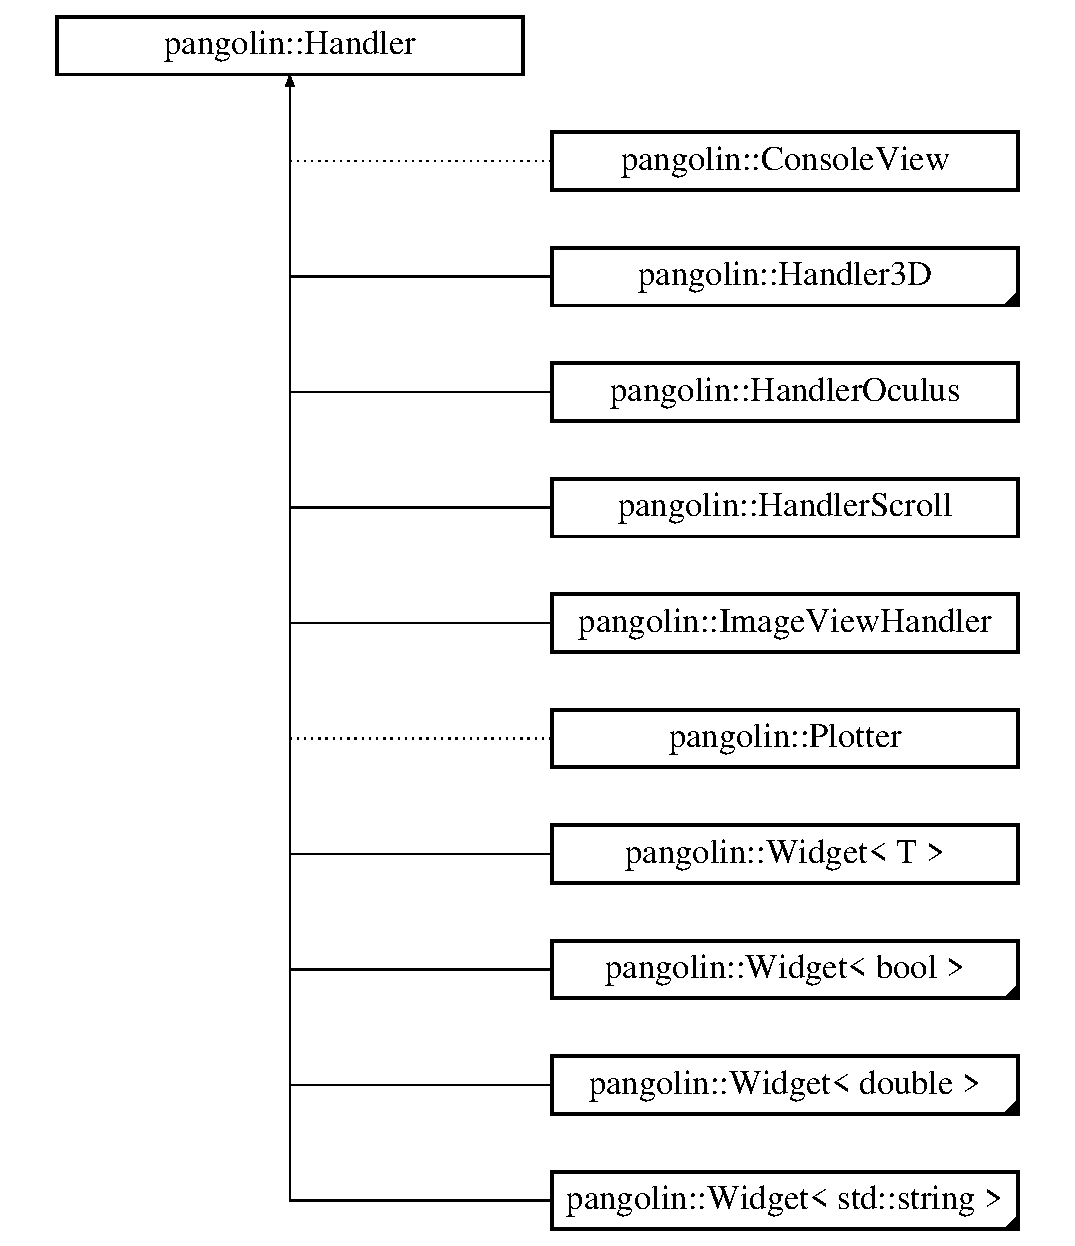
\includegraphics[height=11.000000cm]{structpangolin_1_1_handler}
\end{center}
\end{figure}
\subsection*{Public Member Functions}
\begin{DoxyCompactItemize}
\item 
virtual void {\bfseries Keyboard} (\hyperlink{structpangolin_1_1_view}{View} \&, unsigned char key, int x, int y, bool pressed)\hypertarget{structpangolin_1_1_handler_aa777762ec9ea10276aa030cf6624787e}{}\label{structpangolin_1_1_handler_aa777762ec9ea10276aa030cf6624787e}

\item 
virtual void {\bfseries Mouse} (\hyperlink{structpangolin_1_1_view}{View} \&, Mouse\+Button button, int x, int y, bool pressed, int button\+\_\+state)\hypertarget{structpangolin_1_1_handler_a85b0aa1571091ec54c44a4f59672c4c5}{}\label{structpangolin_1_1_handler_a85b0aa1571091ec54c44a4f59672c4c5}

\item 
virtual void {\bfseries Mouse\+Motion} (\hyperlink{structpangolin_1_1_view}{View} \&, int x, int y, int button\+\_\+state)\hypertarget{structpangolin_1_1_handler_aae505284ea5430cd58b65e350b48b772}{}\label{structpangolin_1_1_handler_aae505284ea5430cd58b65e350b48b772}

\item 
virtual void {\bfseries Passive\+Mouse\+Motion} (\hyperlink{structpangolin_1_1_view}{View} \&, int x, int y, int button\+\_\+state)\hypertarget{structpangolin_1_1_handler_aa4494db317ea8c813d2ca33c430acb4c}{}\label{structpangolin_1_1_handler_aa4494db317ea8c813d2ca33c430acb4c}

\item 
virtual void {\bfseries Special} (\hyperlink{structpangolin_1_1_view}{View} \&, Input\+Special in\+Type, float x, float y, float p1, float p2, float p3, float p4, int button\+\_\+state)\hypertarget{structpangolin_1_1_handler_a3b8234114e97d07bf11b4833038b5f04}{}\label{structpangolin_1_1_handler_a3b8234114e97d07bf11b4833038b5f04}

\end{DoxyCompactItemize}


\subsection{Detailed Description}
Input \hyperlink{structpangolin_1_1_handler}{Handler} base class. 

Virtual methods which recurse into sub-\/displays. 

The documentation for this struct was generated from the following file\+:\begin{DoxyCompactItemize}
\item 
/home/gapo/meng/deps/pangolin/include/pangolin/handler/handler.\+h\end{DoxyCompactItemize}

\hypertarget{structpangolin_1_1_handler3_d}{}\section{pangolin\+:\+:Handler3D Struct Reference}
\label{structpangolin_1_1_handler3_d}\index{pangolin\+::\+Handler3D@{pangolin\+::\+Handler3D}}
Inheritance diagram for pangolin\+:\+:Handler3D\+:\begin{figure}[H]
\begin{center}
\leavevmode
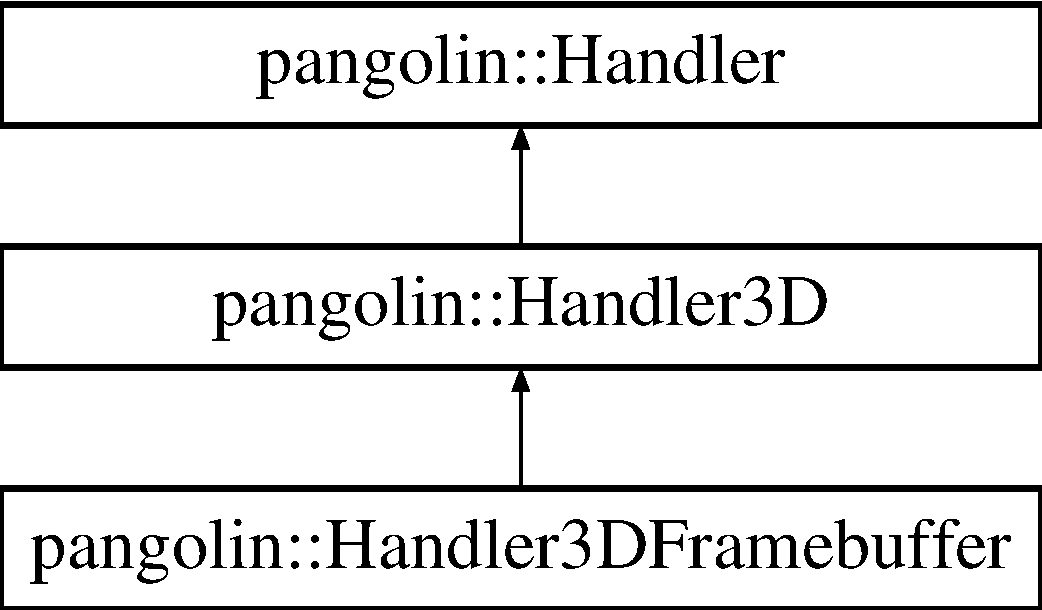
\includegraphics[height=3.000000cm]{structpangolin_1_1_handler3_d}
\end{center}
\end{figure}
\subsection*{Public Member Functions}
\begin{DoxyCompactItemize}
\item 
{\bfseries Handler3D} (\hyperlink{classpangolin_1_1_open_gl_render_state}{Open\+Gl\+Render\+State} \&cam\+\_\+state, Axis\+Direction enforce\+\_\+up=Axis\+None, float trans\+\_\+scale=0.\+01f, float zoom\+\_\+fraction=\+P\+A\+N\+G\+O\+\_\+\+D\+F\+L\+T\+\_\+\+H\+A\+N\+D\+L\+E\+R3\+D\+\_\+\+Z\+F)\hypertarget{structpangolin_1_1_handler3_d_aeb1fcf641c24a7921d2528812be71f6c}{}\label{structpangolin_1_1_handler3_d_aeb1fcf641c24a7921d2528812be71f6c}

\item 
virtual void {\bfseries Get\+Pos\+Normal} (\hyperlink{structpangolin_1_1_view}{View} \&view, int x, int y, G\+Lprecision p\mbox{[}3\mbox{]}, G\+Lprecision Pw\mbox{[}3\mbox{]}, G\+Lprecision Pc\mbox{[}3\mbox{]}, G\+Lprecision n\mbox{[}3\mbox{]}, G\+Lprecision default\+\_\+z=1.\+0)\hypertarget{structpangolin_1_1_handler3_d_a15a0805e015e69eb0723f6c5ffa1cd1f}{}\label{structpangolin_1_1_handler3_d_a15a0805e015e69eb0723f6c5ffa1cd1f}

\item 
void {\bfseries Keyboard} (\hyperlink{structpangolin_1_1_view}{View} \&, unsigned char key, int x, int y, bool pressed)\hypertarget{structpangolin_1_1_handler3_d_afef8f0be6394bdd2ba347f188d6c5cac}{}\label{structpangolin_1_1_handler3_d_afef8f0be6394bdd2ba347f188d6c5cac}

\item 
void {\bfseries Mouse} (\hyperlink{structpangolin_1_1_view}{View} \&, Mouse\+Button button, int x, int y, bool pressed, int button\+\_\+state)\hypertarget{structpangolin_1_1_handler3_d_a915108c717411e1e56777e3a3e3eb626}{}\label{structpangolin_1_1_handler3_d_a915108c717411e1e56777e3a3e3eb626}

\item 
void {\bfseries Mouse\+Motion} (\hyperlink{structpangolin_1_1_view}{View} \&, int x, int y, int button\+\_\+state)\hypertarget{structpangolin_1_1_handler3_d_a71a05eec4a20c7ae8f179ff91f59cbd7}{}\label{structpangolin_1_1_handler3_d_a71a05eec4a20c7ae8f179ff91f59cbd7}

\item 
void {\bfseries Special} (\hyperlink{structpangolin_1_1_view}{View} \&, Input\+Special in\+Type, float x, float y, float p1, float p2, float p3, float p4, int button\+\_\+state)\hypertarget{structpangolin_1_1_handler3_d_a48df691909b0070f063db6c4b5fb6fc3}{}\label{structpangolin_1_1_handler3_d_a48df691909b0070f063db6c4b5fb6fc3}

\end{DoxyCompactItemize}
\subsection*{Protected Attributes}
\begin{DoxyCompactItemize}
\item 
\hyperlink{classpangolin_1_1_open_gl_render_state}{Open\+Gl\+Render\+State} $\ast$ {\bfseries cam\+\_\+state}\hypertarget{structpangolin_1_1_handler3_d_a06a4bcc642f05b6f862de28bdcc7eb2e}{}\label{structpangolin_1_1_handler3_d_a06a4bcc642f05b6f862de28bdcc7eb2e}

\item 
Axis\+Direction {\bfseries enforce\+\_\+up}\hypertarget{structpangolin_1_1_handler3_d_a203fad3e6e2f23764e31a8defd326164}{}\label{structpangolin_1_1_handler3_d_a203fad3e6e2f23764e31a8defd326164}

\item 
float {\bfseries tf}\hypertarget{structpangolin_1_1_handler3_d_a21f13cb711928a706e92a63e2a657043}{}\label{structpangolin_1_1_handler3_d_a21f13cb711928a706e92a63e2a657043}

\item 
float {\bfseries zf}\hypertarget{structpangolin_1_1_handler3_d_a926550a49e53b85efb6a27dbb3674869}{}\label{structpangolin_1_1_handler3_d_a926550a49e53b85efb6a27dbb3674869}

\item 
\hyperlink{structpangolin_1_1_camera_spec}{Camera\+Spec} {\bfseries cameraspec}\hypertarget{structpangolin_1_1_handler3_d_a711ca05ff5438fc1e64f2e3d54fc4be7}{}\label{structpangolin_1_1_handler3_d_a711ca05ff5438fc1e64f2e3d54fc4be7}

\item 
G\+Lprecision {\bfseries last\+\_\+z}\hypertarget{structpangolin_1_1_handler3_d_acaf2d043cde724556982f840fd73d062}{}\label{structpangolin_1_1_handler3_d_acaf2d043cde724556982f840fd73d062}

\item 
float {\bfseries last\+\_\+pos} \mbox{[}2\mbox{]}\hypertarget{structpangolin_1_1_handler3_d_a879a2f62df14b7d29fff9f40eb57155b}{}\label{structpangolin_1_1_handler3_d_a879a2f62df14b7d29fff9f40eb57155b}

\item 
G\+Lprecision {\bfseries rot\+\_\+center} \mbox{[}3\mbox{]}\hypertarget{structpangolin_1_1_handler3_d_a8ec057108e664f92a42c8063bfbc2612}{}\label{structpangolin_1_1_handler3_d_a8ec057108e664f92a42c8063bfbc2612}

\item 
G\+Lprecision {\bfseries p} \mbox{[}3\mbox{]}\hypertarget{structpangolin_1_1_handler3_d_a18db4aec11a163928ee997a5b49abaf0}{}\label{structpangolin_1_1_handler3_d_a18db4aec11a163928ee997a5b49abaf0}

\item 
G\+Lprecision {\bfseries Pw} \mbox{[}3\mbox{]}\hypertarget{structpangolin_1_1_handler3_d_a47843978f86d00d6260c1f68876217ab}{}\label{structpangolin_1_1_handler3_d_a47843978f86d00d6260c1f68876217ab}

\item 
G\+Lprecision {\bfseries Pc} \mbox{[}3\mbox{]}\hypertarget{structpangolin_1_1_handler3_d_a1f48117a4adc74babdf6361dc9d07d81}{}\label{structpangolin_1_1_handler3_d_a1f48117a4adc74babdf6361dc9d07d81}

\item 
G\+Lprecision {\bfseries n} \mbox{[}3\mbox{]}\hypertarget{structpangolin_1_1_handler3_d_a08dd6b6230dd714ce3071b0b94112c00}{}\label{structpangolin_1_1_handler3_d_a08dd6b6230dd714ce3071b0b94112c00}

\end{DoxyCompactItemize}
\subsection*{Static Protected Attributes}
\begin{DoxyCompactItemize}
\item 
static const int {\bfseries hwin} = 8\hypertarget{structpangolin_1_1_handler3_d_aef53600505d7706a0a191a87211da6ce}{}\label{structpangolin_1_1_handler3_d_aef53600505d7706a0a191a87211da6ce}

\end{DoxyCompactItemize}


The documentation for this struct was generated from the following file\+:\begin{DoxyCompactItemize}
\item 
/home/gapo/meng/deps/pangolin/include/pangolin/handler/handler.\+h\end{DoxyCompactItemize}

\hypertarget{structpangolin_1_1_handler3_d_framebuffer}{}\section{pangolin\+:\+:Handler3\+D\+Framebuffer Struct Reference}
\label{structpangolin_1_1_handler3_d_framebuffer}\index{pangolin\+::\+Handler3\+D\+Framebuffer@{pangolin\+::\+Handler3\+D\+Framebuffer}}
Inheritance diagram for pangolin\+:\+:Handler3\+D\+Framebuffer\+:\begin{figure}[H]
\begin{center}
\leavevmode
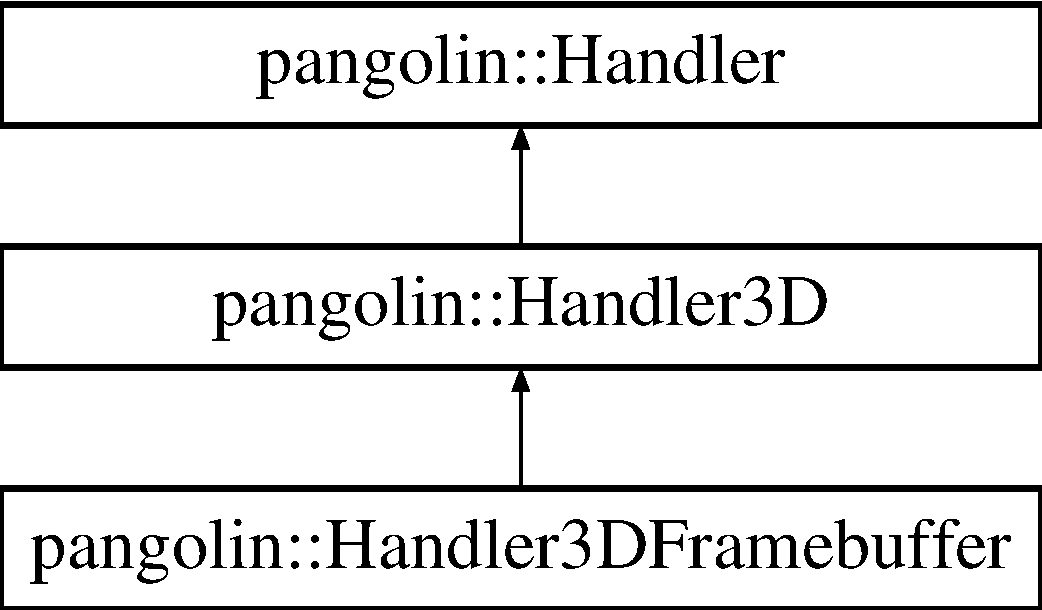
\includegraphics[height=3.000000cm]{structpangolin_1_1_handler3_d_framebuffer}
\end{center}
\end{figure}
\subsection*{Public Member Functions}
\begin{DoxyCompactItemize}
\item 
{\bfseries Handler3\+D\+Framebuffer} (\hyperlink{structpangolin_1_1_gl_framebuffer}{Gl\+Framebuffer} \&fb, \hyperlink{classpangolin_1_1_open_gl_render_state}{pangolin\+::\+Open\+Gl\+Render\+State} \&cam\+\_\+state, pangolin\+::\+Axis\+Direction enforce\+\_\+up=pangolin\+::\+Axis\+None, float trans\+\_\+scale=0.\+01f)\hypertarget{structpangolin_1_1_handler3_d_framebuffer_a2b9665b147e791132a5c7e569ad8c4e3}{}\label{structpangolin_1_1_handler3_d_framebuffer_a2b9665b147e791132a5c7e569ad8c4e3}

\item 
void {\bfseries Get\+Pos\+Normal} (\hyperlink{structpangolin_1_1_view}{pangolin\+::\+View} \&view, int x, int y, G\+Lprecision p\mbox{[}3\mbox{]}, G\+Lprecision Pw\mbox{[}3\mbox{]}, G\+Lprecision Pc\mbox{[}3\mbox{]}, G\+Lprecision\mbox{[}3\mbox{]}, G\+Lprecision default\+\_\+z)\hypertarget{structpangolin_1_1_handler3_d_framebuffer_a2247464e9429db0d7a6661cb0e43da34}{}\label{structpangolin_1_1_handler3_d_framebuffer_a2247464e9429db0d7a6661cb0e43da34}

\end{DoxyCompactItemize}
\subsection*{Protected Attributes}
\begin{DoxyCompactItemize}
\item 
\hyperlink{structpangolin_1_1_gl_framebuffer}{Gl\+Framebuffer} \& {\bfseries fb}\hypertarget{structpangolin_1_1_handler3_d_framebuffer_ab24fefc81aa545e8493b9978ae7d26d1}{}\label{structpangolin_1_1_handler3_d_framebuffer_ab24fefc81aa545e8493b9978ae7d26d1}

\end{DoxyCompactItemize}
\subsection*{Additional Inherited Members}


The documentation for this struct was generated from the following file\+:\begin{DoxyCompactItemize}
\item 
/home/gapo/meng/deps/pangolin/include/pangolin/handler/handler\+\_\+glbuffer.\+h\end{DoxyCompactItemize}

\hypertarget{structpangolin_1_1_handler_oculus}{}\section{pangolin\+:\+:Handler\+Oculus Struct Reference}
\label{structpangolin_1_1_handler_oculus}\index{pangolin\+::\+Handler\+Oculus@{pangolin\+::\+Handler\+Oculus}}
Inheritance diagram for pangolin\+:\+:Handler\+Oculus\+:\begin{figure}[H]
\begin{center}
\leavevmode
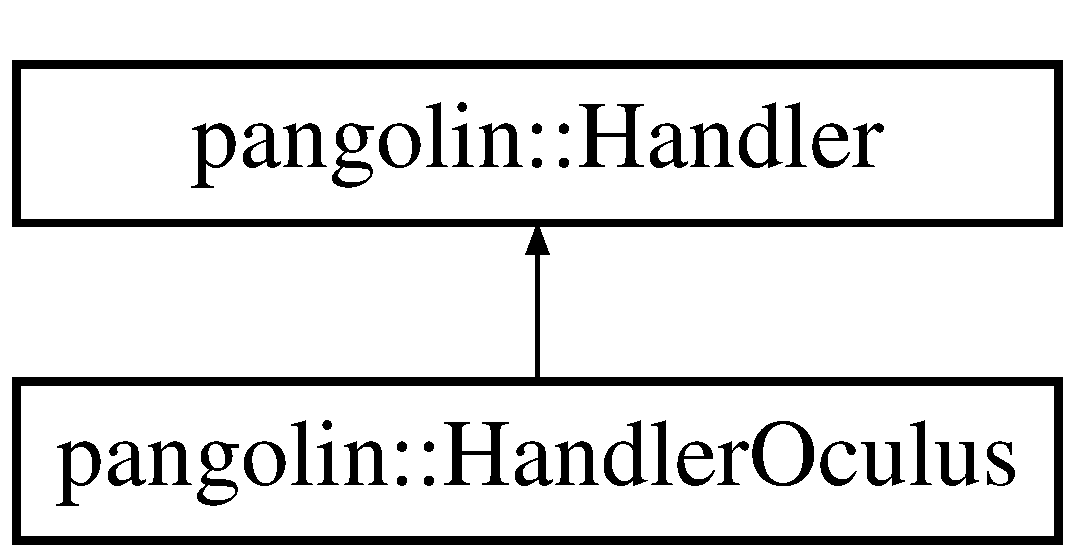
\includegraphics[height=2.000000cm]{structpangolin_1_1_handler_oculus}
\end{center}
\end{figure}
\subsection*{Public Member Functions}
\begin{DoxyCompactItemize}
\item 
{\bfseries Handler\+Oculus} (\hyperlink{classpangolin_1_1_oculus_hud}{Oculus\+Hud} \&oculus, \hyperlink{structpangolin_1_1_handler}{pangolin\+::\+Handler} $\ast$h=0)\hypertarget{structpangolin_1_1_handler_oculus_ab95cd8d69641abfe6661827e8123dba6}{}\label{structpangolin_1_1_handler_oculus_ab95cd8d69641abfe6661827e8123dba6}

\item 
void {\bfseries Keyboard} (\hyperlink{structpangolin_1_1_view}{View} \&, unsigned char key, int x, int y, bool pressed)\hypertarget{structpangolin_1_1_handler_oculus_a14ebc557f794615fa359b26c7771270d}{}\label{structpangolin_1_1_handler_oculus_a14ebc557f794615fa359b26c7771270d}

\item 
void {\bfseries Mouse} (\hyperlink{structpangolin_1_1_view}{View} \&, Mouse\+Button button, int x, int y, bool pressed, int button\+\_\+state)\hypertarget{structpangolin_1_1_handler_oculus_adeb4c87012e2b6c64f1cc8d86037a9f7}{}\label{structpangolin_1_1_handler_oculus_adeb4c87012e2b6c64f1cc8d86037a9f7}

\item 
void {\bfseries Mouse\+Motion} (\hyperlink{structpangolin_1_1_view}{View} \&, int x, int y, int button\+\_\+state)\hypertarget{structpangolin_1_1_handler_oculus_ac5b7b0dcbceefe4bf9c2a316bbd84d62}{}\label{structpangolin_1_1_handler_oculus_ac5b7b0dcbceefe4bf9c2a316bbd84d62}

\item 
void {\bfseries Passive\+Mouse\+Motion} (\hyperlink{structpangolin_1_1_view}{View} \&, int x, int y, int button\+\_\+state)\hypertarget{structpangolin_1_1_handler_oculus_ae60996327ea6d7cffe824afc3a3d822b}{}\label{structpangolin_1_1_handler_oculus_ae60996327ea6d7cffe824afc3a3d822b}

\item 
void {\bfseries Special} (\hyperlink{structpangolin_1_1_view}{View} \&, Input\+Special in\+Type, float x, float y, float p1, float p2, float p3, float p4, int button\+\_\+state)\hypertarget{structpangolin_1_1_handler_oculus_aa5e15c10843162c074eb70a3fc572101}{}\label{structpangolin_1_1_handler_oculus_aa5e15c10843162c074eb70a3fc572101}

\item 
void {\bfseries Set\+Handler} (\hyperlink{structpangolin_1_1_handler}{pangolin\+::\+Handler} $\ast$h)\hypertarget{structpangolin_1_1_handler_oculus_a85249e6e636f10a700b1e653cd18d2aa}{}\label{structpangolin_1_1_handler_oculus_a85249e6e636f10a700b1e653cd18d2aa}

\end{DoxyCompactItemize}
\subsection*{Protected Attributes}
\begin{DoxyCompactItemize}
\item 
\hyperlink{classpangolin_1_1_oculus_hud}{Oculus\+Hud} \& {\bfseries oculus}\hypertarget{structpangolin_1_1_handler_oculus_aafeb2ac80fbdba7aab168f94482e24fe}{}\label{structpangolin_1_1_handler_oculus_aafeb2ac80fbdba7aab168f94482e24fe}

\item 
\hyperlink{structpangolin_1_1_handler}{pangolin\+::\+Handler} $\ast$ {\bfseries handler}\hypertarget{structpangolin_1_1_handler_oculus_af1f064600230aa2bfff882adec8c0569}{}\label{structpangolin_1_1_handler_oculus_af1f064600230aa2bfff882adec8c0569}

\end{DoxyCompactItemize}


The documentation for this struct was generated from the following file\+:\begin{DoxyCompactItemize}
\item 
/home/gapo/meng/deps/pangolin/include/pangolin/hud/oculus\+\_\+hud.\+h\end{DoxyCompactItemize}

\hypertarget{structpangolin_1_1_handler_scroll}{}\section{pangolin\+:\+:Handler\+Scroll Struct Reference}
\label{structpangolin_1_1_handler_scroll}\index{pangolin\+::\+Handler\+Scroll@{pangolin\+::\+Handler\+Scroll}}
Inheritance diagram for pangolin\+:\+:Handler\+Scroll\+:\begin{figure}[H]
\begin{center}
\leavevmode
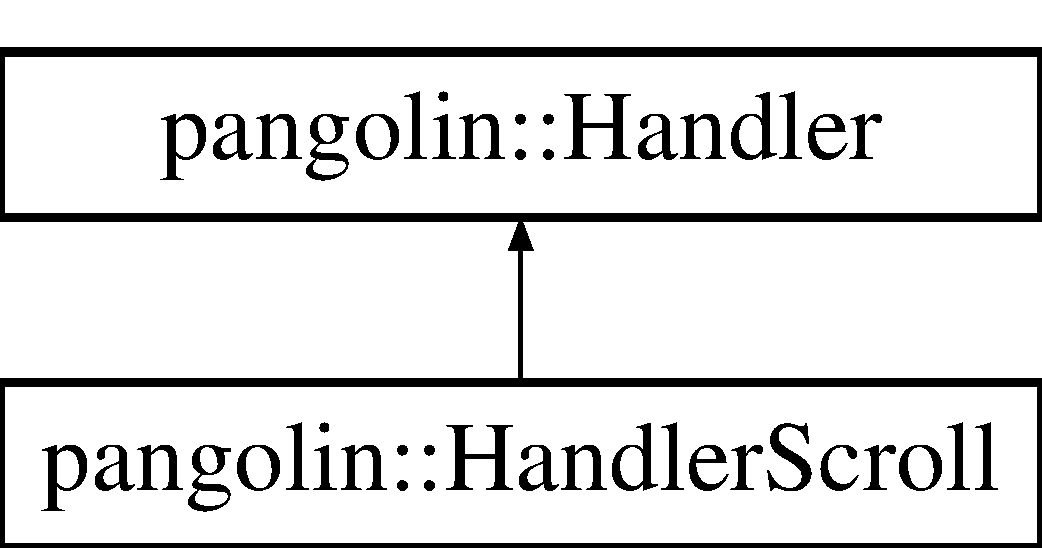
\includegraphics[height=2.000000cm]{structpangolin_1_1_handler_scroll}
\end{center}
\end{figure}
\subsection*{Public Member Functions}
\begin{DoxyCompactItemize}
\item 
void {\bfseries Mouse} (\hyperlink{structpangolin_1_1_view}{View} \&, Mouse\+Button button, int x, int y, bool pressed, int button\+\_\+state)\hypertarget{structpangolin_1_1_handler_scroll_a1242500103211997582034c4691d5ade}{}\label{structpangolin_1_1_handler_scroll_a1242500103211997582034c4691d5ade}

\item 
void {\bfseries Special} (\hyperlink{structpangolin_1_1_view}{View} \&, Input\+Special in\+Type, float x, float y, float p1, float p2, float p3, float p4, int button\+\_\+state)\hypertarget{structpangolin_1_1_handler_scroll_a5327bc5d9f896144f27b4bdf29c96e8e}{}\label{structpangolin_1_1_handler_scroll_a5327bc5d9f896144f27b4bdf29c96e8e}

\end{DoxyCompactItemize}


The documentation for this struct was generated from the following file\+:\begin{DoxyCompactItemize}
\item 
/home/gapo/meng/deps/pangolin/include/pangolin/handler/handler.\+h\end{DoxyCompactItemize}

\hypertarget{structpangolin_1_1_image}{}\section{pangolin\+:\+:Image$<$ T $>$ Struct Template Reference}
\label{structpangolin_1_1_image}\index{pangolin\+::\+Image$<$ T $>$@{pangolin\+::\+Image$<$ T $>$}}
\subsection*{Public Member Functions}
\begin{DoxyCompactItemize}
\item 
{\bfseries Image} (size\+\_\+t w, size\+\_\+t h, size\+\_\+t pitch, T $\ast$ptr)\hypertarget{structpangolin_1_1_image_a843e5cd20521c73cc30a230366512698}{}\label{structpangolin_1_1_image_a843e5cd20521c73cc30a230366512698}

\item 
void {\bfseries Dealloc} ()\hypertarget{structpangolin_1_1_image_a5662d09907544fbb0be7c8aa49e7d7c9}{}\label{structpangolin_1_1_image_a5662d09907544fbb0be7c8aa49e7d7c9}

\item 
void {\bfseries Alloc} (size\+\_\+t w, size\+\_\+t h, size\+\_\+t pitch)\hypertarget{structpangolin_1_1_image_ae06802509f71b4dbdccd89bafac0ee1f}{}\label{structpangolin_1_1_image_ae06802509f71b4dbdccd89bafac0ee1f}

\item 
size\+\_\+t {\bfseries Size\+Bytes} () const \hypertarget{structpangolin_1_1_image_a948128dcb7266100a554f8e639622a1f}{}\label{structpangolin_1_1_image_a948128dcb7266100a554f8e639622a1f}

\item 
size\+\_\+t {\bfseries Area} () const \hypertarget{structpangolin_1_1_image_adbafe72c3158823546b4270336e5a4da}{}\label{structpangolin_1_1_image_adbafe72c3158823546b4270336e5a4da}

\item 
{\footnotesize template$<$typename To $>$ }\\\hyperlink{structpangolin_1_1_image}{Image}$<$ To $>$ {\bfseries Reinterpret} ()\hypertarget{structpangolin_1_1_image_a05f948d07fe2d1e7a4541404f8cdd874}{}\label{structpangolin_1_1_image_a05f948d07fe2d1e7a4541404f8cdd874}

\item 
T $\ast$ {\bfseries Row\+Ptr} (int r)\hypertarget{structpangolin_1_1_image_a2584b77d0c0e51d348493b1186b6d576}{}\label{structpangolin_1_1_image_a2584b77d0c0e51d348493b1186b6d576}

\end{DoxyCompactItemize}
\subsection*{Public Attributes}
\begin{DoxyCompactItemize}
\item 
size\+\_\+t {\bfseries pitch}\hypertarget{structpangolin_1_1_image_a70f559cf9e8398af39d4486439d981e1}{}\label{structpangolin_1_1_image_a70f559cf9e8398af39d4486439d981e1}

\item 
T $\ast$ {\bfseries ptr}\hypertarget{structpangolin_1_1_image_a4c550102df312a014e657dcb076203b4}{}\label{structpangolin_1_1_image_a4c550102df312a014e657dcb076203b4}

\item 
size\+\_\+t {\bfseries w}\hypertarget{structpangolin_1_1_image_a8caedfed88f720430131432fff4dd7dc}{}\label{structpangolin_1_1_image_a8caedfed88f720430131432fff4dd7dc}

\item 
size\+\_\+t {\bfseries h}\hypertarget{structpangolin_1_1_image_af76464116b2127b055e912547be0d507}{}\label{structpangolin_1_1_image_af76464116b2127b055e912547be0d507}

\end{DoxyCompactItemize}


The documentation for this struct was generated from the following file\+:\begin{DoxyCompactItemize}
\item 
/home/gapo/meng/deps/pangolin/include/pangolin/image/image.\+h\end{DoxyCompactItemize}

\hypertarget{structpangolin_1_1_image_dim}{}\section{pangolin\+:\+:Image\+Dim Struct Reference}
\label{structpangolin_1_1_image_dim}\index{pangolin\+::\+Image\+Dim@{pangolin\+::\+Image\+Dim}}
\subsection*{Public Member Functions}
\begin{DoxyCompactItemize}
\item 
{\bfseries Image\+Dim} (size\+\_\+t x, size\+\_\+t y)\hypertarget{structpangolin_1_1_image_dim_ac8b2e1948e217fc2474cc7b7e21009d4}{}\label{structpangolin_1_1_image_dim_ac8b2e1948e217fc2474cc7b7e21009d4}

\end{DoxyCompactItemize}
\subsection*{Public Attributes}
\begin{DoxyCompactItemize}
\item 
size\+\_\+t {\bfseries x}\hypertarget{structpangolin_1_1_image_dim_a5ca02ca0d0999cf41ccb293e54997291}{}\label{structpangolin_1_1_image_dim_a5ca02ca0d0999cf41ccb293e54997291}

\item 
size\+\_\+t {\bfseries y}\hypertarget{structpangolin_1_1_image_dim_a0685f384eb29c0732621506520186752}{}\label{structpangolin_1_1_image_dim_a0685f384eb29c0732621506520186752}

\end{DoxyCompactItemize}


The documentation for this struct was generated from the following file\+:\begin{DoxyCompactItemize}
\item 
/home/gapo/meng/deps/pangolin/include/pangolin/image/image\+\_\+common.\+h\end{DoxyCompactItemize}

\hypertarget{structpangolin_1_1_image_roi}{}\section{pangolin\+:\+:Image\+Roi Struct Reference}
\label{structpangolin_1_1_image_roi}\index{pangolin\+::\+Image\+Roi@{pangolin\+::\+Image\+Roi}}
\subsection*{Public Member Functions}
\begin{DoxyCompactItemize}
\item 
{\bfseries Image\+Roi} (size\+\_\+t x, size\+\_\+t y, size\+\_\+t w, size\+\_\+t h)\hypertarget{structpangolin_1_1_image_roi_aec3d389f6ac61a466f149312d476ba91}{}\label{structpangolin_1_1_image_roi_aec3d389f6ac61a466f149312d476ba91}

\end{DoxyCompactItemize}
\subsection*{Public Attributes}
\begin{DoxyCompactItemize}
\item 
size\+\_\+t {\bfseries x}\hypertarget{structpangolin_1_1_image_roi_a067742f59f0a358f452306400281ba39}{}\label{structpangolin_1_1_image_roi_a067742f59f0a358f452306400281ba39}

\item 
size\+\_\+t {\bfseries y}\hypertarget{structpangolin_1_1_image_roi_ab853dff8d544c0da928e6d5f09df77b9}{}\label{structpangolin_1_1_image_roi_ab853dff8d544c0da928e6d5f09df77b9}

\item 
size\+\_\+t {\bfseries w}\hypertarget{structpangolin_1_1_image_roi_a06209a3b42cfe998f109e23464a2283a}{}\label{structpangolin_1_1_image_roi_a06209a3b42cfe998f109e23464a2283a}

\item 
size\+\_\+t {\bfseries h}\hypertarget{structpangolin_1_1_image_roi_a39dae76e7badc4be12e1fc14948b7cb3}{}\label{structpangolin_1_1_image_roi_a39dae76e7badc4be12e1fc14948b7cb3}

\end{DoxyCompactItemize}


The documentation for this struct was generated from the following file\+:\begin{DoxyCompactItemize}
\item 
/home/gapo/meng/deps/pangolin/include/pangolin/image/image\+\_\+common.\+h\end{DoxyCompactItemize}

\hypertarget{classpangolin_1_1_images_video}{}\section{pangolin\+:\+:Images\+Video Class Reference}
\label{classpangolin_1_1_images_video}\index{pangolin\+::\+Images\+Video@{pangolin\+::\+Images\+Video}}
Inheritance diagram for pangolin\+:\+:Images\+Video\+:\begin{figure}[H]
\begin{center}
\leavevmode
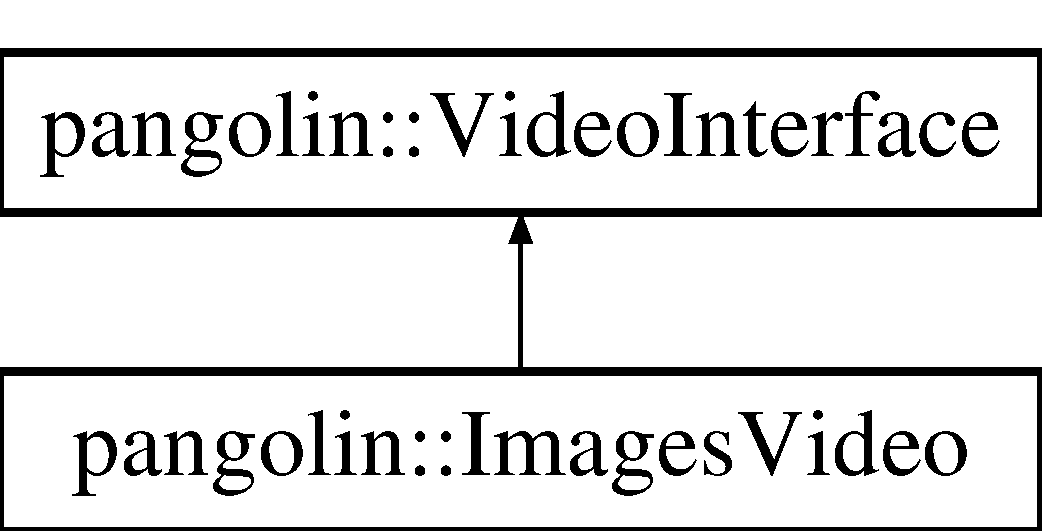
\includegraphics[height=2.000000cm]{classpangolin_1_1_images_video}
\end{center}
\end{figure}
\subsection*{Public Member Functions}
\begin{DoxyCompactItemize}
\item 
{\bfseries Images\+Video} (const std\+::string \&wildcard\+\_\+path)\hypertarget{classpangolin_1_1_images_video_aa39cf8c79c62e7eb89477735b56d5481}{}\label{classpangolin_1_1_images_video_aa39cf8c79c62e7eb89477735b56d5481}

\item 
void \hyperlink{classpangolin_1_1_images_video_a7a6b5ebc7f768b7daefe77c78a1ba2c0}{Start} ()\hypertarget{classpangolin_1_1_images_video_a7a6b5ebc7f768b7daefe77c78a1ba2c0}{}\label{classpangolin_1_1_images_video_a7a6b5ebc7f768b7daefe77c78a1ba2c0}

\begin{DoxyCompactList}\small\item\em Implement \hyperlink{structpangolin_1_1_video_input_a74a2e3e1b87c7cbf9de9bcb39e1df128}{Video\+Input\+::\+Start()} \end{DoxyCompactList}\item 
void \hyperlink{classpangolin_1_1_images_video_a5a4b50d939d7c4745a22e6ededa95ee8}{Stop} ()\hypertarget{classpangolin_1_1_images_video_a5a4b50d939d7c4745a22e6ededa95ee8}{}\label{classpangolin_1_1_images_video_a5a4b50d939d7c4745a22e6ededa95ee8}

\begin{DoxyCompactList}\small\item\em Implement \hyperlink{structpangolin_1_1_video_input_a8945f80194cc7ec9594db7f27e7d09b8}{Video\+Input\+::\+Stop()} \end{DoxyCompactList}\item 
size\+\_\+t \hyperlink{classpangolin_1_1_images_video_a55a141bd595d627a601a1076fb51298c}{Size\+Bytes} () const \hypertarget{classpangolin_1_1_images_video_a55a141bd595d627a601a1076fb51298c}{}\label{classpangolin_1_1_images_video_a55a141bd595d627a601a1076fb51298c}

\begin{DoxyCompactList}\small\item\em Implement \hyperlink{structpangolin_1_1_video_input_a93cee5c33386973a2a51165e6bdcf40b}{Video\+Input\+::\+Size\+Bytes()} \end{DoxyCompactList}\item 
const std\+::vector$<$ \hyperlink{classpangolin_1_1_stream_info}{Stream\+Info} $>$ \& \hyperlink{classpangolin_1_1_images_video_afa5ce7be5d369a860a32db133f618a28}{Streams} () const \hypertarget{classpangolin_1_1_images_video_afa5ce7be5d369a860a32db133f618a28}{}\label{classpangolin_1_1_images_video_afa5ce7be5d369a860a32db133f618a28}

\begin{DoxyCompactList}\small\item\em Implement \hyperlink{structpangolin_1_1_video_input_a9030d775d699c39ab7b7ba378c007c6a}{Video\+Input\+::\+Streams()} \end{DoxyCompactList}\item 
bool \hyperlink{classpangolin_1_1_images_video_a2f305910d2362778bfb96266f3701a75}{Grab\+Next} (unsigned char $\ast$image, bool wait=true)\hypertarget{classpangolin_1_1_images_video_a2f305910d2362778bfb96266f3701a75}{}\label{classpangolin_1_1_images_video_a2f305910d2362778bfb96266f3701a75}

\begin{DoxyCompactList}\small\item\em Implement \hyperlink{structpangolin_1_1_video_input_ad3d8ff59c1ec4139320097e6e1111f32}{Video\+Input\+::\+Grab\+Next()} \end{DoxyCompactList}\item 
bool \hyperlink{classpangolin_1_1_images_video_ad052b1e0e619b077517d3e6bab3c6e95}{Grab\+Newest} (unsigned char $\ast$image, bool wait=true)\hypertarget{classpangolin_1_1_images_video_ad052b1e0e619b077517d3e6bab3c6e95}{}\label{classpangolin_1_1_images_video_ad052b1e0e619b077517d3e6bab3c6e95}

\begin{DoxyCompactList}\small\item\em Implement \hyperlink{structpangolin_1_1_video_input_a4c8ac38e3c6a3f591663aeebf645e4c6}{Video\+Input\+::\+Grab\+Newest()} \end{DoxyCompactList}\end{DoxyCompactItemize}
\subsection*{Protected Types}
\begin{DoxyCompactItemize}
\item 
typedef std\+::vector$<$ \hyperlink{structpangolin_1_1_typed_image}{Typed\+Image} $>$ {\bfseries Frame}\hypertarget{classpangolin_1_1_images_video_ab9c3021c7ee3b34f3edec5365b8fb0f1}{}\label{classpangolin_1_1_images_video_ab9c3021c7ee3b34f3edec5365b8fb0f1}

\end{DoxyCompactItemize}
\subsection*{Protected Member Functions}
\begin{DoxyCompactItemize}
\item 
const std\+::string \& {\bfseries Filename} (size\+\_\+t frame\+Num, size\+\_\+t channel\+Num)\hypertarget{classpangolin_1_1_images_video_ab81f79c9898a7875e9f722a6e256f874}{}\label{classpangolin_1_1_images_video_ab81f79c9898a7875e9f722a6e256f874}

\item 
bool {\bfseries Queue\+Frame} ()\hypertarget{classpangolin_1_1_images_video_aec99bab01c6f66abc063a28ac25039eb}{}\label{classpangolin_1_1_images_video_aec99bab01c6f66abc063a28ac25039eb}

\end{DoxyCompactItemize}
\subsection*{Protected Attributes}
\begin{DoxyCompactItemize}
\item 
std\+::vector$<$ \hyperlink{classpangolin_1_1_stream_info}{Stream\+Info} $>$ {\bfseries streams}\hypertarget{classpangolin_1_1_images_video_a696d2cc58b128dd4033220a91c4f0af4}{}\label{classpangolin_1_1_images_video_a696d2cc58b128dd4033220a91c4f0af4}

\item 
size\+\_\+t {\bfseries size\+\_\+bytes}\hypertarget{classpangolin_1_1_images_video_a2992a5c6e66f2747d09875295cac4400}{}\label{classpangolin_1_1_images_video_a2992a5c6e66f2747d09875295cac4400}

\item 
int {\bfseries num\+\_\+files}\hypertarget{classpangolin_1_1_images_video_a758687525003bba42394f1db963b5502}{}\label{classpangolin_1_1_images_video_a758687525003bba42394f1db963b5502}

\item 
size\+\_\+t {\bfseries num\+\_\+channels}\hypertarget{classpangolin_1_1_images_video_a72baeb13ff3121ba43f33704b6f4e331}{}\label{classpangolin_1_1_images_video_a72baeb13ff3121ba43f33704b6f4e331}

\item 
std\+::vector$<$ std\+::vector$<$ std\+::string $>$ $>$ {\bfseries filenames}\hypertarget{classpangolin_1_1_images_video_a0dea552b8047455a9435440247b9478b}{}\label{classpangolin_1_1_images_video_a0dea552b8047455a9435440247b9478b}

\item 
int {\bfseries num\+\_\+loaded}\hypertarget{classpangolin_1_1_images_video_ae00d18be0b64078830e3e2b4e4661d68}{}\label{classpangolin_1_1_images_video_ae00d18be0b64078830e3e2b4e4661d68}

\item 
std\+::deque$<$ Frame $>$ {\bfseries loaded}\hypertarget{classpangolin_1_1_images_video_adacbd4c70a781a02f8d8042796884fb9}{}\label{classpangolin_1_1_images_video_adacbd4c70a781a02f8d8042796884fb9}

\end{DoxyCompactItemize}


The documentation for this class was generated from the following file\+:\begin{DoxyCompactItemize}
\item 
/home/gapo/meng/deps/pangolin/include/pangolin/video/drivers/images.\+h\end{DoxyCompactItemize}

\hypertarget{classpangolin_1_1_image_view_handler}{}\section{pangolin\+:\+:Image\+View\+Handler Class Reference}
\label{classpangolin_1_1_image_view_handler}\index{pangolin\+::\+Image\+View\+Handler@{pangolin\+::\+Image\+View\+Handler}}
Inheritance diagram for pangolin\+:\+:Image\+View\+Handler\+:\begin{figure}[H]
\begin{center}
\leavevmode
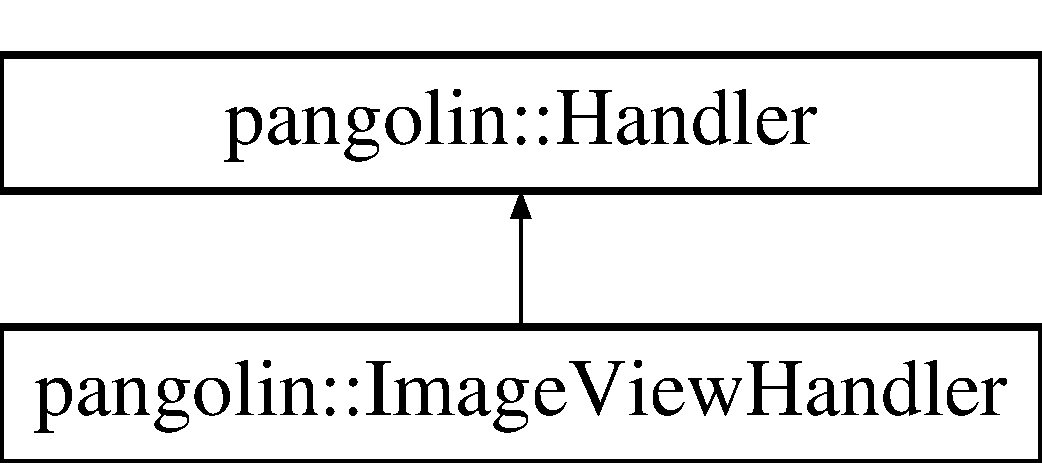
\includegraphics[height=2.000000cm]{classpangolin_1_1_image_view_handler}
\end{center}
\end{figure}
\subsection*{Public Member Functions}
\begin{DoxyCompactItemize}
\item 
{\bfseries Image\+View\+Handler} (size\+\_\+t w, size\+\_\+t h)\hypertarget{classpangolin_1_1_image_view_handler_aa7f8cdfdaaade6428c2d276ce098689d}{}\label{classpangolin_1_1_image_view_handler_aa7f8cdfdaaade6428c2d276ce098689d}

\item 
void {\bfseries Update\+View} ()\hypertarget{classpangolin_1_1_image_view_handler_a71cd8786dfe1e10ef79f75ae9ced686a}{}\label{classpangolin_1_1_image_view_handler_a71cd8786dfe1e10ef79f75ae9ced686a}

\item 
void {\bfseries Screen\+To\+Image} (\hyperlink{structpangolin_1_1_viewport}{Viewport} \&v, int xpix, int ypix, float \&ximg, float \&yimg)\hypertarget{classpangolin_1_1_image_view_handler_ae9aa52388703ee348d663de84c8ef763}{}\label{classpangolin_1_1_image_view_handler_ae9aa52388703ee348d663de84c8ef763}

\item 
bool {\bfseries Use\+NN} () const \hypertarget{classpangolin_1_1_image_view_handler_a762ff523db161a2f04a6d29b84939b19}{}\label{classpangolin_1_1_image_view_handler_a762ff523db161a2f04a6d29b84939b19}

\item 
\hyperlink{structpangolin_1_1_x_y_range}{pangolin\+::\+X\+Y\+Rangef} \& {\bfseries Get\+View\+To\+Render} ()\hypertarget{classpangolin_1_1_image_view_handler_aa66b1586d22f202590d9cf0fdbd55703}{}\label{classpangolin_1_1_image_view_handler_aa66b1586d22f202590d9cf0fdbd55703}

\item 
\hyperlink{structpangolin_1_1_x_y_range}{pangolin\+::\+X\+Y\+Rangef} \& {\bfseries Get\+View} ()\hypertarget{classpangolin_1_1_image_view_handler_a982b562b314393f18f4b7ff52d62e240}{}\label{classpangolin_1_1_image_view_handler_a982b562b314393f18f4b7ff52d62e240}

\item 
\hyperlink{structpangolin_1_1_x_y_range}{pangolin\+::\+X\+Y\+Rangef} \& {\bfseries Get\+Default\+View} ()\hypertarget{classpangolin_1_1_image_view_handler_a1faf88703dafe3576bed8e866e6e471f}{}\label{classpangolin_1_1_image_view_handler_a1faf88703dafe3576bed8e866e6e471f}

\item 
\hyperlink{structpangolin_1_1_x_y_range}{pangolin\+::\+X\+Y\+Rangef} \& {\bfseries Get\+Selection} ()\hypertarget{classpangolin_1_1_image_view_handler_ab0da607c9442f7c83f2993235ea83726}{}\label{classpangolin_1_1_image_view_handler_ab0da607c9442f7c83f2993235ea83726}

\item 
void {\bfseries Set\+View} (const \hyperlink{structpangolin_1_1_x_y_range}{pangolin\+::\+X\+Y\+Rangef} \&range)\hypertarget{classpangolin_1_1_image_view_handler_ac1982a34e41487047fde27a52bfd7be2}{}\label{classpangolin_1_1_image_view_handler_ac1982a34e41487047fde27a52bfd7be2}

\item 
void {\bfseries Set\+View\+Smooth} (const \hyperlink{structpangolin_1_1_x_y_range}{pangolin\+::\+X\+Y\+Rangef} \&range)\hypertarget{classpangolin_1_1_image_view_handler_afe13ee941877a067ec39f80746e05a1f}{}\label{classpangolin_1_1_image_view_handler_afe13ee941877a067ec39f80746e05a1f}

\item 
void {\bfseries Scroll\+View} (float x, float y)\hypertarget{classpangolin_1_1_image_view_handler_a55940ba7720aacfbea9705cb41b57889}{}\label{classpangolin_1_1_image_view_handler_a55940ba7720aacfbea9705cb41b57889}

\item 
void {\bfseries Scroll\+View\+Smooth} (float x, float y)\hypertarget{classpangolin_1_1_image_view_handler_a6244a306668a5f6f0b48b66b3dc2c4a5}{}\label{classpangolin_1_1_image_view_handler_a6244a306668a5f6f0b48b66b3dc2c4a5}

\item 
void {\bfseries Scale\+View} (float x, float y, float cx, float cy)\hypertarget{classpangolin_1_1_image_view_handler_af6226d8cdf1665269a8ad378de2e9e20}{}\label{classpangolin_1_1_image_view_handler_af6226d8cdf1665269a8ad378de2e9e20}

\item 
void {\bfseries Scale\+View\+Smooth} (float x, float y, float cx, float cy)\hypertarget{classpangolin_1_1_image_view_handler_af19f2205ad792ca8460bea63cf8319a5}{}\label{classpangolin_1_1_image_view_handler_af19f2205ad792ca8460bea63cf8319a5}

\item 
void {\bfseries Reset\+View} ()\hypertarget{classpangolin_1_1_image_view_handler_a780292cd2b4a116f59e55a0325c33053}{}\label{classpangolin_1_1_image_view_handler_a780292cd2b4a116f59e55a0325c33053}

\item 
void \hyperlink{classpangolin_1_1_image_view_handler_aaf732a192f393faeea11a7720e8adc5a}{Keyboard} (\hyperlink{structpangolin_1_1_view}{View} \&, unsigned char key, int x, int y, bool pressed) P\+A\+N\+G\+O\+L\+I\+N\+\_\+\+O\+V\+E\+R\+R\+I\+DE\hypertarget{classpangolin_1_1_image_view_handler_aaf732a192f393faeea11a7720e8adc5a}{}\label{classpangolin_1_1_image_view_handler_aaf732a192f393faeea11a7720e8adc5a}

\begin{DoxyCompactList}\small\item\em \hyperlink{structpangolin_1_1_handler}{pangolin\+::\+Handler} \end{DoxyCompactList}\item 
void {\bfseries Mouse} (\hyperlink{structpangolin_1_1_view}{View} \&view, pangolin\+::\+Mouse\+Button button, int x, int y, bool pressed, int button\+\_\+state) P\+A\+N\+G\+O\+L\+I\+N\+\_\+\+O\+V\+E\+R\+R\+I\+DE\hypertarget{classpangolin_1_1_image_view_handler_ad4c5b4537b6efc3c07e62bd54b6eae1a}{}\label{classpangolin_1_1_image_view_handler_ad4c5b4537b6efc3c07e62bd54b6eae1a}

\item 
void {\bfseries Mouse\+Motion} (\hyperlink{structpangolin_1_1_view}{View} \&view, int x, int y, int button\+\_\+state) P\+A\+N\+G\+O\+L\+I\+N\+\_\+\+O\+V\+E\+R\+R\+I\+DE\hypertarget{classpangolin_1_1_image_view_handler_ae18d23acf88cc52eaa91588ab95a7000}{}\label{classpangolin_1_1_image_view_handler_ae18d23acf88cc52eaa91588ab95a7000}

\item 
void {\bfseries Passive\+Mouse\+Motion} (\hyperlink{structpangolin_1_1_view}{View} \&, int x, int y, int button\+\_\+state) P\+A\+N\+G\+O\+L\+I\+N\+\_\+\+O\+V\+E\+R\+R\+I\+DE\hypertarget{classpangolin_1_1_image_view_handler_a1b24d263a2113ea197c007ca8650d91d}{}\label{classpangolin_1_1_image_view_handler_a1b24d263a2113ea197c007ca8650d91d}

\item 
void {\bfseries Special} (\hyperlink{structpangolin_1_1_view}{View} \&view, pangolin\+::\+Input\+Special in\+Type, float x, float y, float p1, float p2, float p3, float p4, int button\+\_\+state) P\+A\+N\+G\+O\+L\+I\+N\+\_\+\+O\+V\+E\+R\+R\+I\+DE\hypertarget{classpangolin_1_1_image_view_handler_ab066f298f7411f97f7d19558d17bb04d}{}\label{classpangolin_1_1_image_view_handler_ab066f298f7411f97f7d19558d17bb04d}

\end{DoxyCompactItemize}
\subsection*{Protected Member Functions}
\begin{DoxyCompactItemize}
\item 
void {\bfseries Fix\+Selection} (\hyperlink{structpangolin_1_1_x_y_range}{X\+Y\+Rangef} \&sel)\hypertarget{classpangolin_1_1_image_view_handler_af2cd9ec553f526094d4fe10f618e1a60}{}\label{classpangolin_1_1_image_view_handler_af2cd9ec553f526094d4fe10f618e1a60}

\item 
void {\bfseries Adjust\+Scale} ()\hypertarget{classpangolin_1_1_image_view_handler_a5e402d7a2de14056babc7d5d6d161e29}{}\label{classpangolin_1_1_image_view_handler_a5e402d7a2de14056babc7d5d6d161e29}

\item 
void {\bfseries Adjust\+Translation} ()\hypertarget{classpangolin_1_1_image_view_handler_af3447c2f5e7615b414f6d0edf50017f7}{}\label{classpangolin_1_1_image_view_handler_af3447c2f5e7615b414f6d0edf50017f7}

\end{DoxyCompactItemize}
\subsection*{Protected Attributes}
\begin{DoxyCompactItemize}
\item 
\hyperlink{classpangolin_1_1_image_view_handler}{Image\+View\+Handler} $\ast$ {\bfseries linked\+\_\+view\+\_\+handler}\hypertarget{classpangolin_1_1_image_view_handler_aa80467ba2cd79056ed89d054e983a5a6}{}\label{classpangolin_1_1_image_view_handler_aa80467ba2cd79056ed89d054e983a5a6}

\item 
\hyperlink{structpangolin_1_1_x_y_range}{pangolin\+::\+X\+Y\+Rangef} {\bfseries rview\+\_\+default}\hypertarget{classpangolin_1_1_image_view_handler_a386fc82476313bbc7188c8feade98731}{}\label{classpangolin_1_1_image_view_handler_a386fc82476313bbc7188c8feade98731}

\item 
\hyperlink{structpangolin_1_1_x_y_range}{pangolin\+::\+X\+Y\+Rangef} {\bfseries rview\+\_\+max}\hypertarget{classpangolin_1_1_image_view_handler_a67fbb3be9aa876c924bf447d5365c510}{}\label{classpangolin_1_1_image_view_handler_a67fbb3be9aa876c924bf447d5365c510}

\item 
\hyperlink{structpangolin_1_1_x_y_range}{pangolin\+::\+X\+Y\+Rangef} {\bfseries rview}\hypertarget{classpangolin_1_1_image_view_handler_af938850ed37f18bffebd5e677e48e26c}{}\label{classpangolin_1_1_image_view_handler_af938850ed37f18bffebd5e677e48e26c}

\item 
\hyperlink{structpangolin_1_1_x_y_range}{pangolin\+::\+X\+Y\+Rangef} {\bfseries target}\hypertarget{classpangolin_1_1_image_view_handler_a4f4a235a71d4eab79e18d366bbb0afee}{}\label{classpangolin_1_1_image_view_handler_a4f4a235a71d4eab79e18d366bbb0afee}

\item 
\hyperlink{structpangolin_1_1_x_y_range}{pangolin\+::\+X\+Y\+Rangef} {\bfseries selection}\hypertarget{classpangolin_1_1_image_view_handler_a5e217a0d039fe255e0dbe9120fff5937}{}\label{classpangolin_1_1_image_view_handler_a5e217a0d039fe255e0dbe9120fff5937}

\item 
float {\bfseries hover} \mbox{[}2\mbox{]}\hypertarget{classpangolin_1_1_image_view_handler_aa8631b215f9389edfbc6eaae538857ca}{}\label{classpangolin_1_1_image_view_handler_aa8631b215f9389edfbc6eaae538857ca}

\item 
int {\bfseries last\+\_\+mouse\+\_\+pos} \mbox{[}2\mbox{]}\hypertarget{classpangolin_1_1_image_view_handler_a3f22d95a5791d23ba7ce37bdb3144bcc}{}\label{classpangolin_1_1_image_view_handler_a3f22d95a5791d23ba7ce37bdb3144bcc}

\item 
bool {\bfseries use\+\_\+nn}\hypertarget{classpangolin_1_1_image_view_handler_ad9fd47c04c99be51275a46a4e2ef995c}{}\label{classpangolin_1_1_image_view_handler_ad9fd47c04c99be51275a46a4e2ef995c}

\end{DoxyCompactItemize}
\subsection*{Static Protected Attributes}
\begin{DoxyCompactItemize}
\item 
static \hyperlink{classpangolin_1_1_image_view_handler}{Image\+View\+Handler} $\ast$ {\bfseries to\+\_\+link} = 0\hypertarget{classpangolin_1_1_image_view_handler_a0172fec7cd8510058bcfd00409b681ff}{}\label{classpangolin_1_1_image_view_handler_a0172fec7cd8510058bcfd00409b681ff}

\item 
static float {\bfseries animate\+\_\+factor} = 1.\+0f / 2.\+0f\hypertarget{classpangolin_1_1_image_view_handler_a2f187b0a682e5ced6d6830c217de5d73}{}\label{classpangolin_1_1_image_view_handler_a2f187b0a682e5ced6d6830c217de5d73}

\end{DoxyCompactItemize}


The documentation for this class was generated from the following file\+:\begin{DoxyCompactItemize}
\item 
/home/gapo/meng/deps/pangolin/include/pangolin/handler/handler\+\_\+image.\+h\end{DoxyCompactItemize}

\hypertarget{classpangolin_1_1json_1_1input}{}\section{pangolin\+:\+:json\+:\+:input$<$ Iter $>$ Class Template Reference}
\label{classpangolin_1_1json_1_1input}\index{pangolin\+::json\+::input$<$ Iter $>$@{pangolin\+::json\+::input$<$ Iter $>$}}
\subsection*{Public Member Functions}
\begin{DoxyCompactItemize}
\item 
{\bfseries input} (const Iter \&first, const Iter \&last)\hypertarget{classpangolin_1_1json_1_1input_a842ddc016079248aeb19b630f31674e0}{}\label{classpangolin_1_1json_1_1input_a842ddc016079248aeb19b630f31674e0}

\item 
int {\bfseries getc} ()\hypertarget{classpangolin_1_1json_1_1input_ad14af8ff8ef5dffaa5d9e039e60d3586}{}\label{classpangolin_1_1json_1_1input_ad14af8ff8ef5dffaa5d9e039e60d3586}

\item 
void {\bfseries ungetc} ()\hypertarget{classpangolin_1_1json_1_1input_a790d33d589614d6766325a82661c2c8c}{}\label{classpangolin_1_1json_1_1input_a790d33d589614d6766325a82661c2c8c}

\item 
Iter {\bfseries cur} () const \hypertarget{classpangolin_1_1json_1_1input_a83996aff4a9751cabbd55355a2f2506f}{}\label{classpangolin_1_1json_1_1input_a83996aff4a9751cabbd55355a2f2506f}

\item 
int {\bfseries line} () const \hypertarget{classpangolin_1_1json_1_1input_a0909f2bd0b1829c2c79a6c86c26f5d66}{}\label{classpangolin_1_1json_1_1input_a0909f2bd0b1829c2c79a6c86c26f5d66}

\item 
void {\bfseries skip\+\_\+ws} ()\hypertarget{classpangolin_1_1json_1_1input_a5f96bcc84bbfa4e5bc5132cd469b6913}{}\label{classpangolin_1_1json_1_1input_a5f96bcc84bbfa4e5bc5132cd469b6913}

\item 
bool {\bfseries expect} (int expect)\hypertarget{classpangolin_1_1json_1_1input_abb2dd067eea684f0504d1b018dff3a54}{}\label{classpangolin_1_1json_1_1input_abb2dd067eea684f0504d1b018dff3a54}

\item 
bool {\bfseries match} (const std\+::string \&pattern)\hypertarget{classpangolin_1_1json_1_1input_a88215cb203775294d1544784245fb28d}{}\label{classpangolin_1_1json_1_1input_a88215cb203775294d1544784245fb28d}

\end{DoxyCompactItemize}
\subsection*{Protected Attributes}
\begin{DoxyCompactItemize}
\item 
Iter {\bfseries cur\+\_\+}\hypertarget{classpangolin_1_1json_1_1input_aec2f56bf8a745cea869fdc0b827461da}{}\label{classpangolin_1_1json_1_1input_aec2f56bf8a745cea869fdc0b827461da}

\item 
Iter {\bfseries end\+\_\+}\hypertarget{classpangolin_1_1json_1_1input_a596b64d7e2a1840768ac50ed795b6c8a}{}\label{classpangolin_1_1json_1_1input_a596b64d7e2a1840768ac50ed795b6c8a}

\item 
int {\bfseries last\+\_\+ch\+\_\+}\hypertarget{classpangolin_1_1json_1_1input_a93f0fe1c1757e801b91ca9251fb5b6f3}{}\label{classpangolin_1_1json_1_1input_a93f0fe1c1757e801b91ca9251fb5b6f3}

\item 
bool {\bfseries ungot\+\_\+}\hypertarget{classpangolin_1_1json_1_1input_a5ef4aedb53fa2f67603cc2bf8fd86f70}{}\label{classpangolin_1_1json_1_1input_a5ef4aedb53fa2f67603cc2bf8fd86f70}

\item 
int {\bfseries line\+\_\+}\hypertarget{classpangolin_1_1json_1_1input_a6b44d960882efce51998657716c307fc}{}\label{classpangolin_1_1json_1_1input_a6b44d960882efce51998657716c307fc}

\end{DoxyCompactItemize}


The documentation for this class was generated from the following file\+:\begin{DoxyCompactItemize}
\item 
/home/gapo/meng/deps/pangolin/include/pangolin/utils/picojson.\+h\end{DoxyCompactItemize}

\hypertarget{structpangolin_1_1_input_record_repeat}{}\section{pangolin\+:\+:Input\+Record\+Repeat Struct Reference}
\label{structpangolin_1_1_input_record_repeat}\index{pangolin\+::\+Input\+Record\+Repeat@{pangolin\+::\+Input\+Record\+Repeat}}
\subsection*{Public Member Functions}
\begin{DoxyCompactItemize}
\item 
{\bfseries Input\+Record\+Repeat} (const std\+::string \&var\+\_\+record\+\_\+prefix)\hypertarget{structpangolin_1_1_input_record_repeat_a9f0f47525b3526fad774aa2efdc848d6}{}\label{structpangolin_1_1_input_record_repeat_a9f0f47525b3526fad774aa2efdc848d6}

\item 
void {\bfseries Set\+Index} (int id)\hypertarget{structpangolin_1_1_input_record_repeat_a29cf2f137e26c3d5722fa6a484d5404d}{}\label{structpangolin_1_1_input_record_repeat_a29cf2f137e26c3d5722fa6a484d5404d}

\item 
void {\bfseries Record} ()\hypertarget{structpangolin_1_1_input_record_repeat_a04a55473913c5c6afea83758ceee71aa}{}\label{structpangolin_1_1_input_record_repeat_a04a55473913c5c6afea83758ceee71aa}

\item 
void {\bfseries Stop} ()\hypertarget{structpangolin_1_1_input_record_repeat_a267062d01aade988c257927f7082ea22}{}\label{structpangolin_1_1_input_record_repeat_a267062d01aade988c257927f7082ea22}

\item 
void {\bfseries Load\+Buffer} (const std\+::string \&filename)\hypertarget{structpangolin_1_1_input_record_repeat_a13921fa8a4430258d4f005781e080c25}{}\label{structpangolin_1_1_input_record_repeat_a13921fa8a4430258d4f005781e080c25}

\item 
void {\bfseries Save\+Buffer} (const std\+::string \&filename)\hypertarget{structpangolin_1_1_input_record_repeat_a11cb5cdf60a4c0b99dddbefa701252d4}{}\label{structpangolin_1_1_input_record_repeat_a11cb5cdf60a4c0b99dddbefa701252d4}

\item 
void {\bfseries Clear\+Buffer} ()\hypertarget{structpangolin_1_1_input_record_repeat_a89b0d7951948c06c6efc55124e6a47f4}{}\label{structpangolin_1_1_input_record_repeat_a89b0d7951948c06c6efc55124e6a47f4}

\item 
void {\bfseries Play\+Buffer} ()\hypertarget{structpangolin_1_1_input_record_repeat_ac9abc5882d61da21fa39d970e485be5f}{}\label{structpangolin_1_1_input_record_repeat_ac9abc5882d61da21fa39d970e485be5f}

\item 
void {\bfseries Play\+Buffer} (size\+\_\+t start, size\+\_\+t end)\hypertarget{structpangolin_1_1_input_record_repeat_ad4fe53211558dae32bc527b078254f37}{}\label{structpangolin_1_1_input_record_repeat_ad4fe53211558dae32bc527b078254f37}

\item 
void {\bfseries Update\+Variable} (const std\+::string \&name)\hypertarget{structpangolin_1_1_input_record_repeat_a838ce7811bc025c2e40495afd1544390}{}\label{structpangolin_1_1_input_record_repeat_a838ce7811bc025c2e40495afd1544390}

\item 
{\footnotesize template$<$typename T $>$ }\\void {\bfseries Update\+Variable} (const \hyperlink{classpangolin_1_1_var}{Var}$<$ T $>$ \&var)\hypertarget{structpangolin_1_1_input_record_repeat_a34e3e49c066ccc9f34b84e9cb81d1d4f}{}\label{structpangolin_1_1_input_record_repeat_a34e3e49c066ccc9f34b84e9cb81d1d4f}

\item 
size\+\_\+t {\bfseries Size} ()\hypertarget{structpangolin_1_1_input_record_repeat_ab0f6abc691786215269ec7ff7fe25b46}{}\label{structpangolin_1_1_input_record_repeat_ab0f6abc691786215269ec7ff7fe25b46}

\end{DoxyCompactItemize}
\subsection*{Static Protected Member Functions}
\begin{DoxyCompactItemize}
\item 
static void {\bfseries Gui\+Var\+Changed} (void $\ast$data, const std\+::string \&name, \hyperlink{classpangolin_1_1_var_value_generic}{Var\+Value\+Generic} \&var)\hypertarget{structpangolin_1_1_input_record_repeat_a0b98eb9703c760ea23833ae1a96f35e7}{}\label{structpangolin_1_1_input_record_repeat_a0b98eb9703c760ea23833ae1a96f35e7}

\end{DoxyCompactItemize}
\subsection*{Protected Attributes}
\begin{DoxyCompactItemize}
\item 
bool {\bfseries record}\hypertarget{structpangolin_1_1_input_record_repeat_a1f63548705a399f0822fe7e9d169ffe1}{}\label{structpangolin_1_1_input_record_repeat_a1f63548705a399f0822fe7e9d169ffe1}

\item 
bool {\bfseries play}\hypertarget{structpangolin_1_1_input_record_repeat_ae6e3684d6237e1c326a29cd32f89625f}{}\label{structpangolin_1_1_input_record_repeat_ae6e3684d6237e1c326a29cd32f89625f}

\item 
int {\bfseries index}\hypertarget{structpangolin_1_1_input_record_repeat_a889dd65e62e50bfbc8ff1c1304d3abac}{}\label{structpangolin_1_1_input_record_repeat_a889dd65e62e50bfbc8ff1c1304d3abac}

\item 
std\+::ofstream {\bfseries file}\hypertarget{structpangolin_1_1_input_record_repeat_a4a360df06ee1a733c0312f1aa1fe7e09}{}\label{structpangolin_1_1_input_record_repeat_a4a360df06ee1a733c0312f1aa1fe7e09}

\item 
std\+::string {\bfseries filename}\hypertarget{structpangolin_1_1_input_record_repeat_a5633fa57616e7276201fadbd73675b7f}{}\label{structpangolin_1_1_input_record_repeat_a5633fa57616e7276201fadbd73675b7f}

\item 
std\+::list$<$ \hyperlink{structpangolin_1_1_frame_input}{Frame\+Input} $>$ {\bfseries play\+\_\+queue}\hypertarget{structpangolin_1_1_input_record_repeat_a0fdad6c5b32c4bad4fa3e5413d857f79}{}\label{structpangolin_1_1_input_record_repeat_a0fdad6c5b32c4bad4fa3e5413d857f79}

\item 
std\+::list$<$ \hyperlink{structpangolin_1_1_frame_input}{Frame\+Input} $>$ {\bfseries record\+\_\+queue}\hypertarget{structpangolin_1_1_input_record_repeat_a73adce0f3218524c899d8a9a56ec11e5}{}\label{structpangolin_1_1_input_record_repeat_a73adce0f3218524c899d8a9a56ec11e5}

\end{DoxyCompactItemize}


The documentation for this struct was generated from the following file\+:\begin{DoxyCompactItemize}
\item 
/home/gapo/meng/deps/pangolin/include/pangolin/var/input\+\_\+record\+\_\+repeat.\+h\end{DoxyCompactItemize}

\hypertarget{structpangolin_1_1json_1_1last__error__t}{}\section{pangolin\+:\+:json\+:\+:last\+\_\+error\+\_\+t$<$ T $>$ Struct Template Reference}
\label{structpangolin_1_1json_1_1last__error__t}\index{pangolin\+::json\+::last\+\_\+error\+\_\+t$<$ T $>$@{pangolin\+::json\+::last\+\_\+error\+\_\+t$<$ T $>$}}
\subsection*{Static Public Attributes}
\begin{DoxyCompactItemize}
\item 
static std\+::string {\bfseries s}\hypertarget{structpangolin_1_1json_1_1last__error__t_ae8982a740d8bef01d589c7997baec5ef}{}\label{structpangolin_1_1json_1_1last__error__t_ae8982a740d8bef01d589c7997baec5ef}

\end{DoxyCompactItemize}


The documentation for this struct was generated from the following file\+:\begin{DoxyCompactItemize}
\item 
/home/gapo/meng/deps/pangolin/include/pangolin/utils/picojson.\+h\end{DoxyCompactItemize}

\hypertarget{structpangolin_1_1_console_view_1_1_line}{}\section{pangolin\+:\+:Console\+View\+:\+:Line Struct Reference}
\label{structpangolin_1_1_console_view_1_1_line}\index{pangolin\+::\+Console\+View\+::\+Line@{pangolin\+::\+Console\+View\+::\+Line}}
\subsection*{Public Member Functions}
\begin{DoxyCompactItemize}
\item 
{\bfseries Line} (const \hyperlink{classpangolin_1_1_gl_text}{Gl\+Text} \&text, Console\+Line\+Type linetype=Console\+Line\+Type\+Cmd)\hypertarget{structpangolin_1_1_console_view_1_1_line_a9dc68674dc2f808ac2a2019ab4925a6b}{}\label{structpangolin_1_1_console_view_1_1_line_a9dc68674dc2f808ac2a2019ab4925a6b}

\end{DoxyCompactItemize}
\subsection*{Public Attributes}
\begin{DoxyCompactItemize}
\item 
\hyperlink{classpangolin_1_1_gl_text}{Gl\+Text} {\bfseries text}\hypertarget{structpangolin_1_1_console_view_1_1_line_ab0700d6bb1eb86d59522dc8fe95a2df1}{}\label{structpangolin_1_1_console_view_1_1_line_ab0700d6bb1eb86d59522dc8fe95a2df1}

\item 
Console\+Line\+Type {\bfseries linetype}\hypertarget{structpangolin_1_1_console_view_1_1_line_a0ad2f48d2a8532ea64a21092d89b6086}{}\label{structpangolin_1_1_console_view_1_1_line_a0ad2f48d2a8532ea64a21092d89b6086}

\end{DoxyCompactItemize}


The documentation for this struct was generated from the following file\+:\begin{DoxyCompactItemize}
\item 
/home/gapo/meng/deps/pangolin/include/pangolin/console/Console\+View.\+h\end{DoxyCompactItemize}

\hypertarget{structpangolin_1_1_marker}{}\section{pangolin\+:\+:Marker Struct Reference}
\label{structpangolin_1_1_marker}\index{pangolin\+::\+Marker@{pangolin\+::\+Marker}}
\subsection*{Public Types}
\begin{DoxyCompactItemize}
\item 
enum {\bfseries Direction} \{ {\bfseries Horizontal}, 
{\bfseries Vertical}
 \}\hypertarget{structpangolin_1_1_marker_a1f53af7b3403a08f920f013c1d3dccaa}{}\label{structpangolin_1_1_marker_a1f53af7b3403a08f920f013c1d3dccaa}

\item 
enum {\bfseries Equality} \{ {\bfseries Less\+Than} = -\/1, 
{\bfseries Equal} = 0, 
{\bfseries Greater\+Than} = 1
 \}\hypertarget{structpangolin_1_1_marker_a3d67b40df94c6cd17eacdc9b1d74f1f4}{}\label{structpangolin_1_1_marker_a3d67b40df94c6cd17eacdc9b1d74f1f4}

\end{DoxyCompactItemize}
\subsection*{Public Member Functions}
\begin{DoxyCompactItemize}
\item 
{\bfseries Marker} (Direction d, float value, Equality leg=Equal, \hyperlink{structpangolin_1_1_colour}{Colour} c=\hyperlink{structpangolin_1_1_colour}{Colour}())\hypertarget{structpangolin_1_1_marker_ab2c7bf7d05b62f2b862f8d3427849746}{}\label{structpangolin_1_1_marker_ab2c7bf7d05b62f2b862f8d3427849746}

\end{DoxyCompactItemize}
\subsection*{Public Attributes}
\begin{DoxyCompactItemize}
\item 
Direction {\bfseries direction}\hypertarget{structpangolin_1_1_marker_a8e4515b4b344503e36cb09ed85f40fd8}{}\label{structpangolin_1_1_marker_a8e4515b4b344503e36cb09ed85f40fd8}

\item 
float {\bfseries value}\hypertarget{structpangolin_1_1_marker_a7e205b2755f77558cf2f672c8b55b708}{}\label{structpangolin_1_1_marker_a7e205b2755f77558cf2f672c8b55b708}

\item 
Equality {\bfseries leg}\hypertarget{structpangolin_1_1_marker_af5f198d565165ef282febe79995923ba}{}\label{structpangolin_1_1_marker_af5f198d565165ef282febe79995923ba}

\item 
\hyperlink{structpangolin_1_1_colour}{Colour} {\bfseries colour}\hypertarget{structpangolin_1_1_marker_a94c61df14eaa7a2ed0ae248169b5a7ce}{}\label{structpangolin_1_1_marker_a94c61df14eaa7a2ed0ae248169b5a7ce}

\end{DoxyCompactItemize}


The documentation for this struct was generated from the following file\+:\begin{DoxyCompactItemize}
\item 
/home/gapo/meng/deps/pangolin/include/pangolin/plot/plotter.\+h\end{DoxyCompactItemize}

\hypertarget{structpangolin_1_1_new_var_callback}{}\section{pangolin\+:\+:New\+Var\+Callback Struct Reference}
\label{structpangolin_1_1_new_var_callback}\index{pangolin\+::\+New\+Var\+Callback@{pangolin\+::\+New\+Var\+Callback}}
\subsection*{Public Member Functions}
\begin{DoxyCompactItemize}
\item 
{\bfseries New\+Var\+Callback} (const std\+::string \&filter, New\+Var\+Callback\+Fn fn, void $\ast$data)\hypertarget{structpangolin_1_1_new_var_callback_af65ff1828148da0910a794b3a9230295}{}\label{structpangolin_1_1_new_var_callback_af65ff1828148da0910a794b3a9230295}

\end{DoxyCompactItemize}
\subsection*{Public Attributes}
\begin{DoxyCompactItemize}
\item 
std\+::string {\bfseries filter}\hypertarget{structpangolin_1_1_new_var_callback_a5bb6fadcd45ce9bb6ff5c418064d122d}{}\label{structpangolin_1_1_new_var_callback_a5bb6fadcd45ce9bb6ff5c418064d122d}

\item 
New\+Var\+Callback\+Fn {\bfseries fn}\hypertarget{structpangolin_1_1_new_var_callback_a6cc6dc2abb4c03e7f4f05b4ac245d4bb}{}\label{structpangolin_1_1_new_var_callback_a6cc6dc2abb4c03e7f4f05b4ac245d4bb}

\item 
void $\ast$ {\bfseries data}\hypertarget{structpangolin_1_1_new_var_callback_a2c5a89ad64d6226e26d256bc86cb53f9}{}\label{structpangolin_1_1_new_var_callback_a2c5a89ad64d6226e26d256bc86cb53f9}

\end{DoxyCompactItemize}


The documentation for this struct was generated from the following file\+:\begin{DoxyCompactItemize}
\item 
/home/gapo/meng/deps/pangolin/include/pangolin/var/varstate.\+h\end{DoxyCompactItemize}

\hypertarget{structpangolin_1_1json_1_1null}{}\section{pangolin\+:\+:json\+:\+:null Struct Reference}
\label{structpangolin_1_1json_1_1null}\index{pangolin\+::json\+::null@{pangolin\+::json\+::null}}


The documentation for this struct was generated from the following file\+:\begin{DoxyCompactItemize}
\item 
/home/gapo/meng/deps/pangolin/include/pangolin/utils/picojson.\+h\end{DoxyCompactItemize}

\hypertarget{classpangolin_1_1json_1_1null__parse__context}{}\section{pangolin\+:\+:json\+:\+:null\+\_\+parse\+\_\+context Class Reference}
\label{classpangolin_1_1json_1_1null__parse__context}\index{pangolin\+::json\+::null\+\_\+parse\+\_\+context@{pangolin\+::json\+::null\+\_\+parse\+\_\+context}}
\subsection*{Classes}
\begin{DoxyCompactItemize}
\item 
struct \hyperlink{structpangolin_1_1json_1_1null__parse__context_1_1dummy__str}{dummy\+\_\+str}
\end{DoxyCompactItemize}
\subsection*{Public Member Functions}
\begin{DoxyCompactItemize}
\item 
bool {\bfseries set\+\_\+null} ()\hypertarget{classpangolin_1_1json_1_1null__parse__context_a31bde18a5e217d3915d94bf513ca27ad}{}\label{classpangolin_1_1json_1_1null__parse__context_a31bde18a5e217d3915d94bf513ca27ad}

\item 
bool {\bfseries set\+\_\+bool} (bool)\hypertarget{classpangolin_1_1json_1_1null__parse__context_aae394c11180911f2b36b1e87373b6c0a}{}\label{classpangolin_1_1json_1_1null__parse__context_aae394c11180911f2b36b1e87373b6c0a}

\item 
bool {\bfseries set\+\_\+int64} (int64\+\_\+t)\hypertarget{classpangolin_1_1json_1_1null__parse__context_a2bacec0a063c83769d474fe839fd4f9b}{}\label{classpangolin_1_1json_1_1null__parse__context_a2bacec0a063c83769d474fe839fd4f9b}

\item 
bool {\bfseries set\+\_\+number} (double)\hypertarget{classpangolin_1_1json_1_1null__parse__context_a0522daf76a26b977cd9e9d42372dcc47}{}\label{classpangolin_1_1json_1_1null__parse__context_a0522daf76a26b977cd9e9d42372dcc47}

\item 
{\footnotesize template$<$typename Iter $>$ }\\bool {\bfseries parse\+\_\+string} (\hyperlink{classpangolin_1_1json_1_1input}{input}$<$ Iter $>$ \&in)\hypertarget{classpangolin_1_1json_1_1null__parse__context_a821f494ff14dd8ef58fb64d2b2aeb286}{}\label{classpangolin_1_1json_1_1null__parse__context_a821f494ff14dd8ef58fb64d2b2aeb286}

\item 
bool {\bfseries parse\+\_\+array\+\_\+start} ()\hypertarget{classpangolin_1_1json_1_1null__parse__context_ac4c51f70fac6ed02766719829c2a4bde}{}\label{classpangolin_1_1json_1_1null__parse__context_ac4c51f70fac6ed02766719829c2a4bde}

\item 
{\footnotesize template$<$typename Iter $>$ }\\bool {\bfseries parse\+\_\+array\+\_\+item} (\hyperlink{classpangolin_1_1json_1_1input}{input}$<$ Iter $>$ \&in, size\+\_\+t)\hypertarget{classpangolin_1_1json_1_1null__parse__context_ac34150003894503e4799e88164af510c}{}\label{classpangolin_1_1json_1_1null__parse__context_ac34150003894503e4799e88164af510c}

\item 
bool {\bfseries parse\+\_\+array\+\_\+stop} (size\+\_\+t)\hypertarget{classpangolin_1_1json_1_1null__parse__context_a93ef1fbae52bd2647c0625471dd0ec46}{}\label{classpangolin_1_1json_1_1null__parse__context_a93ef1fbae52bd2647c0625471dd0ec46}

\item 
bool {\bfseries parse\+\_\+object\+\_\+start} ()\hypertarget{classpangolin_1_1json_1_1null__parse__context_aba82f08620faa437902b09ec75e86e62}{}\label{classpangolin_1_1json_1_1null__parse__context_aba82f08620faa437902b09ec75e86e62}

\item 
{\footnotesize template$<$typename Iter $>$ }\\bool {\bfseries parse\+\_\+object\+\_\+item} (\hyperlink{classpangolin_1_1json_1_1input}{input}$<$ Iter $>$ \&in, const std\+::string \&)\hypertarget{classpangolin_1_1json_1_1null__parse__context_a397548466a3b59a02c36a597d866826e}{}\label{classpangolin_1_1json_1_1null__parse__context_a397548466a3b59a02c36a597d866826e}

\end{DoxyCompactItemize}


The documentation for this class was generated from the following file\+:\begin{DoxyCompactItemize}
\item 
/home/gapo/meng/deps/pangolin/include/pangolin/utils/picojson.\+h\end{DoxyCompactItemize}

\hypertarget{classpangolin_1_1_oculus_hud}{}\section{pangolin\+:\+:Oculus\+Hud Class Reference}
\label{classpangolin_1_1_oculus_hud}\index{pangolin\+::\+Oculus\+Hud@{pangolin\+::\+Oculus\+Hud}}
Inheritance diagram for pangolin\+:\+:Oculus\+Hud\+:\begin{figure}[H]
\begin{center}
\leavevmode
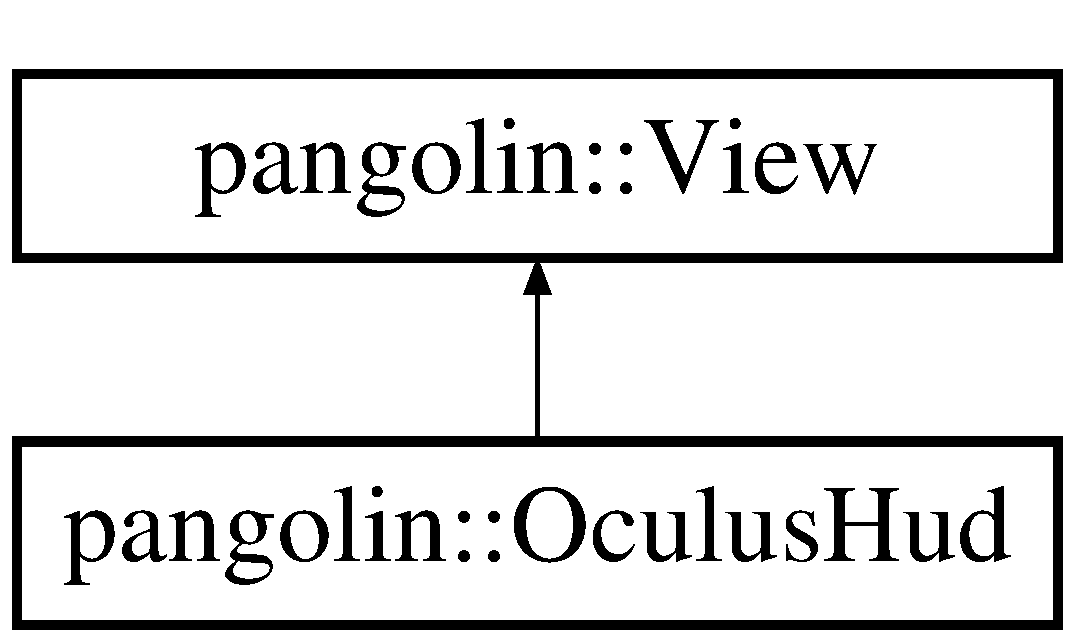
\includegraphics[height=2.000000cm]{classpangolin_1_1_oculus_hud}
\end{center}
\end{figure}
\subsection*{Public Member Functions}
\begin{DoxyCompactItemize}
\item 
void \hyperlink{classpangolin_1_1_oculus_hud_a54d2f4e6a2e7919a7808de679d490197}{Render} ()
\begin{DoxyCompactList}\small\item\em Perform any automatic rendering for this \hyperlink{structpangolin_1_1_view}{View}. \end{DoxyCompactList}\item 
void {\bfseries Render\+Framebuffer} ()\hypertarget{classpangolin_1_1_oculus_hud_accfc28351dfcec0b0feeba79567fc13a}{}\label{classpangolin_1_1_oculus_hud_accfc28351dfcec0b0feeba79567fc13a}

\item 
void {\bfseries Set\+Handler} (\hyperlink{structpangolin_1_1_handler}{Handler} $\ast$handler)\hypertarget{classpangolin_1_1_oculus_hud_a7c9add08ddbcfc7e6f2b6039397f1822}{}\label{classpangolin_1_1_oculus_hud_a7c9add08ddbcfc7e6f2b6039397f1822}

\item 
void {\bfseries Set\+Params} (float focal\+Length, float lens\+X\+Offset, float eye\+\_\+y, float eye\+\_\+z)\hypertarget{classpangolin_1_1_oculus_hud_afc6aa548d662ce07b3f695061d103eee}{}\label{classpangolin_1_1_oculus_hud_afc6aa548d662ce07b3f695061d103eee}

\item 
O\+V\+R\+::\+H\+M\+D\+Info \& {\bfseries Hmd\+Info} ()\hypertarget{classpangolin_1_1_oculus_hud_a4e21b86c96587ccdbceb1b17d7f428cb}{}\label{classpangolin_1_1_oculus_hud_a4e21b86c96587ccdbceb1b17d7f428cb}

\item 
unsigned int {\bfseries Num\+Eyes} () const \hypertarget{classpangolin_1_1_oculus_hud_ac0913f2f49cf75b5cbb656eaf663520f}{}\label{classpangolin_1_1_oculus_hud_ac0913f2f49cf75b5cbb656eaf663520f}

\item 
\hyperlink{structpangolin_1_1_view}{View} \& {\bfseries Common\+View} ()\hypertarget{classpangolin_1_1_oculus_hud_a916b141f2da3690d03908e1e4be6d537}{}\label{classpangolin_1_1_oculus_hud_a916b141f2da3690d03908e1e4be6d537}

\item 
\hyperlink{structpangolin_1_1_open_gl_matrix}{Open\+Gl\+Matrix} {\bfseries Head\+Transform} ()\hypertarget{classpangolin_1_1_oculus_hud_aee116324d9d14f1562889870aaff77e4}{}\label{classpangolin_1_1_oculus_hud_aee116324d9d14f1562889870aaff77e4}

\item 
\hyperlink{structpangolin_1_1_open_gl_matrix}{Open\+Gl\+Matrix} {\bfseries Head\+Transform\+Delta} ()\hypertarget{classpangolin_1_1_oculus_hud_a5c463962d92226e5b191ab2ae1267637}{}\label{classpangolin_1_1_oculus_hud_a5c463962d92226e5b191ab2ae1267637}

\item 
\hyperlink{structpangolin_1_1_gl_framebuffer}{pangolin\+::\+Gl\+Framebuffer} \& {\bfseries Framebuffer} ()\hypertarget{classpangolin_1_1_oculus_hud_af9a942e57b0dba2c94fd603e51c7cb2e}{}\label{classpangolin_1_1_oculus_hud_af9a942e57b0dba2c94fd603e51c7cb2e}

\item 
\hyperlink{classpangolin_1_1_open_gl_render_state}{pangolin\+::\+Open\+Gl\+Render\+State} \& {\bfseries Default\+Render\+State} ()\hypertarget{classpangolin_1_1_oculus_hud_a21047ecf09f66559c59bdad00eb27548}{}\label{classpangolin_1_1_oculus_hud_a21047ecf09f66559c59bdad00eb27548}

\item 
void {\bfseries Unwarp\+Point} (unsigned int view, const float in\mbox{[}2\mbox{]}, float out\mbox{[}2\mbox{]})\hypertarget{classpangolin_1_1_oculus_hud_a4472de0642895806dbfa535d0af7e644}{}\label{classpangolin_1_1_oculus_hud_a4472de0642895806dbfa535d0af7e644}

\end{DoxyCompactItemize}
\subsection*{Protected Member Functions}
\begin{DoxyCompactItemize}
\item 
void {\bfseries Initialise\+Oculus} ()\hypertarget{classpangolin_1_1_oculus_hud_ad161153f89a6bbfce769efa980585c4b}{}\label{classpangolin_1_1_oculus_hud_ad161153f89a6bbfce769efa980585c4b}

\item 
void {\bfseries Initialise\+Framebuffer} ()\hypertarget{classpangolin_1_1_oculus_hud_a937f73c34d008a976ef47f32dcd3d933}{}\label{classpangolin_1_1_oculus_hud_a937f73c34d008a976ef47f32dcd3d933}

\item 
void {\bfseries Initialise\+Shader} ()\hypertarget{classpangolin_1_1_oculus_hud_ace91affe6f6bbcfbae004e2fcbe27966}{}\label{classpangolin_1_1_oculus_hud_ace91affe6f6bbcfbae004e2fcbe27966}

\end{DoxyCompactItemize}
\subsection*{Protected Attributes}
\begin{DoxyCompactItemize}
\item 
\hyperlink{classpangolin_1_1_gl_texture}{pangolin\+::\+Gl\+Texture} {\bfseries colourbuffer}\hypertarget{classpangolin_1_1_oculus_hud_ad0cd74bddbfbc4bbeadd81e7760deb75}{}\label{classpangolin_1_1_oculus_hud_ad0cd74bddbfbc4bbeadd81e7760deb75}

\item 
\hyperlink{structpangolin_1_1_gl_render_buffer}{pangolin\+::\+Gl\+Render\+Buffer} {\bfseries depthbuffer}\hypertarget{classpangolin_1_1_oculus_hud_a1564a899d2e2495ddcdc10034288297f}{}\label{classpangolin_1_1_oculus_hud_a1564a899d2e2495ddcdc10034288297f}

\item 
\hyperlink{structpangolin_1_1_gl_framebuffer}{pangolin\+::\+Gl\+Framebuffer} {\bfseries framebuffer}\hypertarget{classpangolin_1_1_oculus_hud_ac10d425452278fdc229b540ba8d119cf}{}\label{classpangolin_1_1_oculus_hud_ac10d425452278fdc229b540ba8d119cf}

\item 
\hyperlink{classpangolin_1_1_gl_sl_program}{pangolin\+::\+Gl\+Sl\+Program} {\bfseries occ}\hypertarget{classpangolin_1_1_oculus_hud_a540a8535d6268ce0540364e855f9a481}{}\label{classpangolin_1_1_oculus_hud_a540a8535d6268ce0540364e855f9a481}

\item 
bool {\bfseries post\+\_\+unwarp}\hypertarget{classpangolin_1_1_oculus_hud_a6e5868da547b481215fb41f148724b23}{}\label{classpangolin_1_1_oculus_hud_a6e5868da547b481215fb41f148724b23}

\item 
O\+V\+R\+::\+Ptr$<$ O\+V\+R\+::\+Device\+Manager $>$ {\bfseries p\+Manager}\hypertarget{classpangolin_1_1_oculus_hud_ab7d20ae316c5357fbf7db0207def720a}{}\label{classpangolin_1_1_oculus_hud_ab7d20ae316c5357fbf7db0207def720a}

\item 
O\+V\+R\+::\+Ptr$<$ O\+V\+R\+::\+H\+M\+D\+Device $>$ {\bfseries p\+H\+MD}\hypertarget{classpangolin_1_1_oculus_hud_a795539bbc027b24eaa811c7580f9b7ac}{}\label{classpangolin_1_1_oculus_hud_a795539bbc027b24eaa811c7580f9b7ac}

\item 
O\+V\+R\+::\+Ptr$<$ O\+V\+R\+::\+Sensor\+Device $>$ {\bfseries p\+Sensor}\hypertarget{classpangolin_1_1_oculus_hud_aeb13baa12019e3716ba7cbe2baaba3b1}{}\label{classpangolin_1_1_oculus_hud_aeb13baa12019e3716ba7cbe2baaba3b1}

\item 
boostd\+::shared\+\_\+ptr$<$ O\+V\+R\+::\+Sensor\+Fusion $>$ {\bfseries p\+Fusion\+Result}\hypertarget{classpangolin_1_1_oculus_hud_a830ee6e33a93079a9dc0ccba022e32da}{}\label{classpangolin_1_1_oculus_hud_a830ee6e33a93079a9dc0ccba022e32da}

\item 
O\+V\+R\+::\+H\+M\+D\+Info {\bfseries H\+MD}\hypertarget{classpangolin_1_1_oculus_hud_a30b1761772efda31b1517e7a42ab7dff}{}\label{classpangolin_1_1_oculus_hud_a30b1761772efda31b1517e7a42ab7dff}

\item 
O\+V\+R\+::\+Util\+::\+Render\+::\+Stereo\+Config {\bfseries stereo}\hypertarget{classpangolin_1_1_oculus_hud_a3a52b5f33ea26d50ac54cb53f9f14acf}{}\label{classpangolin_1_1_oculus_hud_a3a52b5f33ea26d50ac54cb53f9f14acf}

\item 
\hyperlink{structpangolin_1_1_view}{View} {\bfseries eyeview} \mbox{[}2\mbox{]}\hypertarget{classpangolin_1_1_oculus_hud_a06e6516d4341cdc2d5b98c2897a069a2}{}\label{classpangolin_1_1_oculus_hud_a06e6516d4341cdc2d5b98c2897a069a2}

\item 
\hyperlink{structpangolin_1_1_view}{View} {\bfseries common}\hypertarget{classpangolin_1_1_oculus_hud_a834a1c748899ecc8e9090ea8cf14e801}{}\label{classpangolin_1_1_oculus_hud_a834a1c748899ecc8e9090ea8cf14e801}

\item 
\hyperlink{classpangolin_1_1_open_gl_render_state}{pangolin\+::\+Open\+Gl\+Render\+State} {\bfseries default\+\_\+cam}\hypertarget{classpangolin_1_1_oculus_hud_ae2286e2e274d229b74e8e31570068e39}{}\label{classpangolin_1_1_oculus_hud_ae2286e2e274d229b74e8e31570068e39}

\item 
\hyperlink{structpangolin_1_1_handler_oculus}{Handler\+Oculus} {\bfseries handler}\hypertarget{classpangolin_1_1_oculus_hud_acecb8fcd708b07cb6f6ec714b0c19584}{}\label{classpangolin_1_1_oculus_hud_acecb8fcd708b07cb6f6ec714b0c19584}

\item 
\hyperlink{structpangolin_1_1_open_gl_matrix}{Open\+Gl\+Matrix} {\bfseries T\+\_\+oc}\hypertarget{classpangolin_1_1_oculus_hud_ae9807a880fc6da480dab82371ecf8702}{}\label{classpangolin_1_1_oculus_hud_ae9807a880fc6da480dab82371ecf8702}

\end{DoxyCompactItemize}
\subsection*{Static Protected Attributes}
\begin{DoxyCompactItemize}
\item 
static const char $\ast$ {\bfseries Post\+Process\+Full\+Frag\+Shader\+Src}\hypertarget{classpangolin_1_1_oculus_hud_a2299def7aff61105bdca9aa351358234}{}\label{classpangolin_1_1_oculus_hud_a2299def7aff61105bdca9aa351358234}

\end{DoxyCompactItemize}
\subsection*{Additional Inherited Members}


\subsection{Member Function Documentation}
\index{pangolin\+::\+Oculus\+Hud@{pangolin\+::\+Oculus\+Hud}!Render@{Render}}
\index{Render@{Render}!pangolin\+::\+Oculus\+Hud@{pangolin\+::\+Oculus\+Hud}}
\subsubsection[{\texorpdfstring{Render()}{Render()}}]{\setlength{\rightskip}{0pt plus 5cm}void pangolin\+::\+Oculus\+Hud\+::\+Render (
\begin{DoxyParamCaption}
{}
\end{DoxyParamCaption}
)\hspace{0.3cm}{\ttfamily [virtual]}}\hypertarget{classpangolin_1_1_oculus_hud_a54d2f4e6a2e7919a7808de679d490197}{}\label{classpangolin_1_1_oculus_hud_a54d2f4e6a2e7919a7808de679d490197}


Perform any automatic rendering for this \hyperlink{structpangolin_1_1_view}{View}. 

Default implementation simply instructs children to render themselves. 

Reimplemented from \hyperlink{structpangolin_1_1_view_a15bf43d7ebc4ebe4e02cba572f0d49ba}{pangolin\+::\+View}.



The documentation for this class was generated from the following file\+:\begin{DoxyCompactItemize}
\item 
/home/gapo/meng/deps/pangolin/include/pangolin/hud/oculus\+\_\+hud.\+h\end{DoxyCompactItemize}

\hypertarget{structpangolin_1_1_open_gl_matrix}{}\section{pangolin\+:\+:Open\+Gl\+Matrix Struct Reference}
\label{structpangolin_1_1_open_gl_matrix}\index{pangolin\+::\+Open\+Gl\+Matrix@{pangolin\+::\+Open\+Gl\+Matrix}}


Object representing Open\+Gl Matrix.  




{\ttfamily \#include $<$opengl\+\_\+render\+\_\+state.\+h$>$}

Inheritance diagram for pangolin\+:\+:Open\+Gl\+Matrix\+:\begin{figure}[H]
\begin{center}
\leavevmode
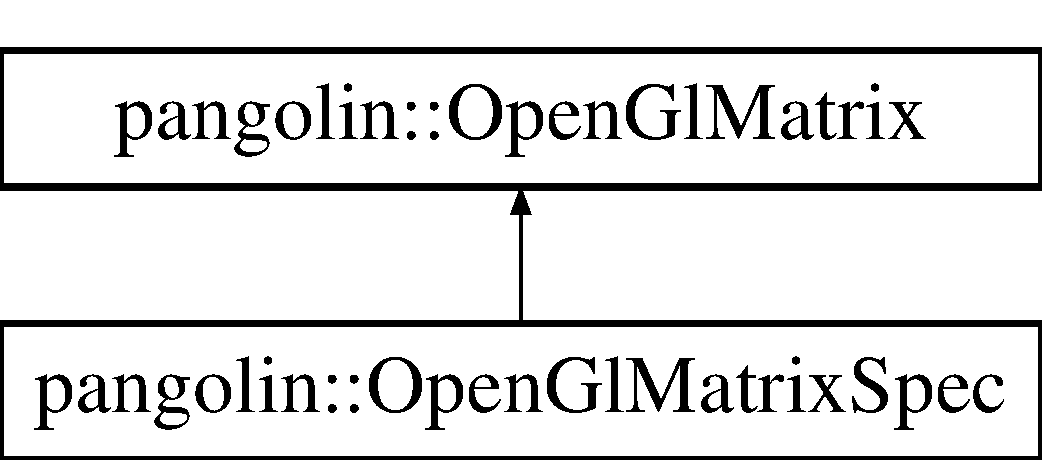
\includegraphics[height=2.000000cm]{structpangolin_1_1_open_gl_matrix}
\end{center}
\end{figure}
\subsection*{Public Member Functions}
\begin{DoxyCompactItemize}
\item 
void {\bfseries Load} () const \hypertarget{structpangolin_1_1_open_gl_matrix_a83ae68b1e8eab15fda9fcafa690f4a3c}{}\label{structpangolin_1_1_open_gl_matrix_a83ae68b1e8eab15fda9fcafa690f4a3c}

\item 
void {\bfseries Multiply} () const \hypertarget{structpangolin_1_1_open_gl_matrix_af267fbcfce8403014fbb7d644fb402de}{}\label{structpangolin_1_1_open_gl_matrix_af267fbcfce8403014fbb7d644fb402de}

\item 
void {\bfseries Set\+Identity} ()\hypertarget{structpangolin_1_1_open_gl_matrix_adef1ce3332e71a64dd0e79eab8a977e9}{}\label{structpangolin_1_1_open_gl_matrix_adef1ce3332e71a64dd0e79eab8a977e9}

\item 
\hyperlink{structpangolin_1_1_open_gl_matrix}{Open\+Gl\+Matrix} {\bfseries Transpose} () const \hypertarget{structpangolin_1_1_open_gl_matrix_a82afc932bcb2a52d012dda1731aaa3ca}{}\label{structpangolin_1_1_open_gl_matrix_a82afc932bcb2a52d012dda1731aaa3ca}

\item 
\hyperlink{structpangolin_1_1_open_gl_matrix}{Open\+Gl\+Matrix} {\bfseries Inverse} () const \hypertarget{structpangolin_1_1_open_gl_matrix_a4366c077b1fd985eac61d468a4a182e6}{}\label{structpangolin_1_1_open_gl_matrix_a4366c077b1fd985eac61d468a4a182e6}

\item 
G\+Lprecision \& {\bfseries operator()} (int r, int c)\hypertarget{structpangolin_1_1_open_gl_matrix_a3cc99d0824e479d8cc5e329b3aea412d}{}\label{structpangolin_1_1_open_gl_matrix_a3cc99d0824e479d8cc5e329b3aea412d}

\item 
G\+Lprecision {\bfseries operator()} (int r, int c) const \hypertarget{structpangolin_1_1_open_gl_matrix_aaffce32d503f5d2e712bf41f06b883c3}{}\label{structpangolin_1_1_open_gl_matrix_aaffce32d503f5d2e712bf41f06b883c3}

\end{DoxyCompactItemize}
\subsection*{Static Public Member Functions}
\begin{DoxyCompactItemize}
\item 
static \hyperlink{structpangolin_1_1_open_gl_matrix}{Open\+Gl\+Matrix} {\bfseries Translate} (G\+Lprecision x, G\+Lprecision y, G\+Lprecision z)\hypertarget{structpangolin_1_1_open_gl_matrix_ae017fce9e537593d2b09c0340313e829}{}\label{structpangolin_1_1_open_gl_matrix_ae017fce9e537593d2b09c0340313e829}

\item 
static \hyperlink{structpangolin_1_1_open_gl_matrix}{Open\+Gl\+Matrix} {\bfseries Scale} (G\+Lprecision x, G\+Lprecision y, G\+Lprecision z)\hypertarget{structpangolin_1_1_open_gl_matrix_a051479f6724f6335a58631743c4509a8}{}\label{structpangolin_1_1_open_gl_matrix_a051479f6724f6335a58631743c4509a8}

\item 
static \hyperlink{structpangolin_1_1_open_gl_matrix}{Open\+Gl\+Matrix} {\bfseries RotateX} (G\+Lprecision theta\+\_\+rad)\hypertarget{structpangolin_1_1_open_gl_matrix_a44a0a9c518623f98588c98496b6b1707}{}\label{structpangolin_1_1_open_gl_matrix_a44a0a9c518623f98588c98496b6b1707}

\item 
static \hyperlink{structpangolin_1_1_open_gl_matrix}{Open\+Gl\+Matrix} {\bfseries RotateY} (G\+Lprecision theta\+\_\+rad)\hypertarget{structpangolin_1_1_open_gl_matrix_add3c228151866d9fcd7acc7a10c30bc4}{}\label{structpangolin_1_1_open_gl_matrix_add3c228151866d9fcd7acc7a10c30bc4}

\item 
static \hyperlink{structpangolin_1_1_open_gl_matrix}{Open\+Gl\+Matrix} {\bfseries RotateZ} (G\+Lprecision theta\+\_\+rad)\hypertarget{structpangolin_1_1_open_gl_matrix_a71af7938cdd77aac099f7e429e8865f9}{}\label{structpangolin_1_1_open_gl_matrix_a71af7938cdd77aac099f7e429e8865f9}

\item 
{\footnotesize template$<$typename P $>$ }\\static \hyperlink{structpangolin_1_1_open_gl_matrix}{Open\+Gl\+Matrix} {\bfseries Col\+Major4x4} (const P $\ast$col\+\_\+major\+\_\+4x4)\hypertarget{structpangolin_1_1_open_gl_matrix_a4ba1ff2a3188442d0e43f30c075aae58}{}\label{structpangolin_1_1_open_gl_matrix_a4ba1ff2a3188442d0e43f30c075aae58}

\end{DoxyCompactItemize}
\subsection*{Public Attributes}
\begin{DoxyCompactItemize}
\item 
G\+Lprecision {\bfseries m} \mbox{[}16\mbox{]}\hypertarget{structpangolin_1_1_open_gl_matrix_a662660308aa8a3dfb2aee1abc143d56c}{}\label{structpangolin_1_1_open_gl_matrix_a662660308aa8a3dfb2aee1abc143d56c}

\end{DoxyCompactItemize}


\subsection{Detailed Description}
Object representing Open\+Gl Matrix. 

The documentation for this struct was generated from the following file\+:\begin{DoxyCompactItemize}
\item 
/home/gapo/meng/deps/pangolin/include/pangolin/display/opengl\+\_\+render\+\_\+state.\+h\end{DoxyCompactItemize}

\hypertarget{structpangolin_1_1_open_gl_matrix_spec}{}\section{pangolin\+:\+:Open\+Gl\+Matrix\+Spec Struct Reference}
\label{structpangolin_1_1_open_gl_matrix_spec}\index{pangolin\+::\+Open\+Gl\+Matrix\+Spec@{pangolin\+::\+Open\+Gl\+Matrix\+Spec}}


Deprecated.  




{\ttfamily \#include $<$opengl\+\_\+render\+\_\+state.\+h$>$}

Inheritance diagram for pangolin\+:\+:Open\+Gl\+Matrix\+Spec\+:\begin{figure}[H]
\begin{center}
\leavevmode
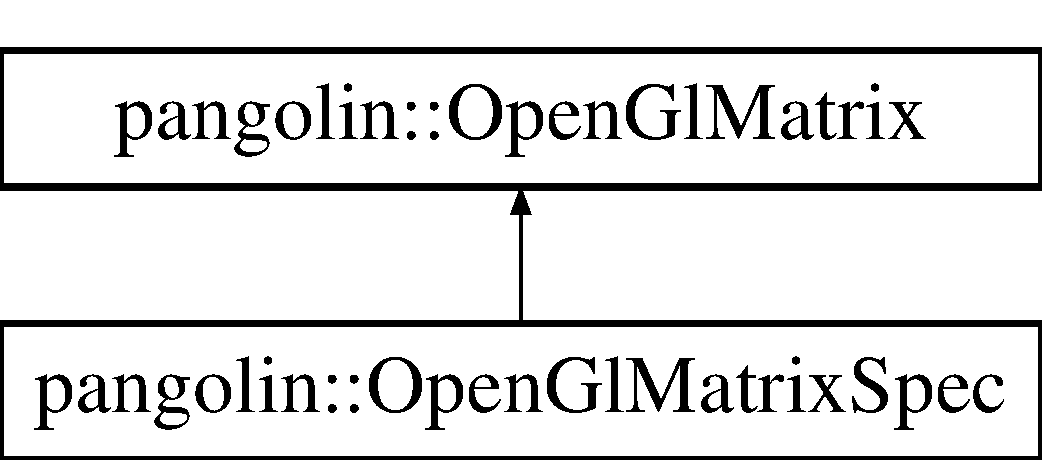
\includegraphics[height=2.000000cm]{structpangolin_1_1_open_gl_matrix_spec}
\end{center}
\end{figure}
\subsection*{Public Attributes}
\begin{DoxyCompactItemize}
\item 
Open\+Gl\+Stack {\bfseries type}\hypertarget{structpangolin_1_1_open_gl_matrix_spec_a1154276433df8ca2d6a4838c12af00f9}{}\label{structpangolin_1_1_open_gl_matrix_spec_a1154276433df8ca2d6a4838c12af00f9}

\end{DoxyCompactItemize}
\subsection*{Additional Inherited Members}


\subsection{Detailed Description}
Deprecated. 

The documentation for this struct was generated from the following file\+:\begin{DoxyCompactItemize}
\item 
/home/gapo/meng/deps/pangolin/include/pangolin/display/opengl\+\_\+render\+\_\+state.\+h\end{DoxyCompactItemize}

\hypertarget{classpangolin_1_1_open_gl_render_state}{}\section{pangolin\+:\+:Open\+Gl\+Render\+State Class Reference}
\label{classpangolin_1_1_open_gl_render_state}\index{pangolin\+::\+Open\+Gl\+Render\+State@{pangolin\+::\+Open\+Gl\+Render\+State}}


Object representing attached Open\+Gl Matrices / transforms.  




{\ttfamily \#include $<$opengl\+\_\+render\+\_\+state.\+h$>$}

\subsection*{Public Member Functions}
\begin{DoxyCompactItemize}
\item 
{\bfseries Open\+Gl\+Render\+State} (const \hyperlink{structpangolin_1_1_open_gl_matrix}{Open\+Gl\+Matrix} \&projection\+\_\+matrix)\hypertarget{classpangolin_1_1_open_gl_render_state_a9a6d5a0d832f71c3a0cacf8b1f98f10c}{}\label{classpangolin_1_1_open_gl_render_state_a9a6d5a0d832f71c3a0cacf8b1f98f10c}

\item 
{\bfseries Open\+Gl\+Render\+State} (const \hyperlink{structpangolin_1_1_open_gl_matrix}{Open\+Gl\+Matrix} \&projection\+\_\+matrix, const \hyperlink{structpangolin_1_1_open_gl_matrix}{Open\+Gl\+Matrix} \&modelview\+\_\+matrix)\hypertarget{classpangolin_1_1_open_gl_render_state_a1ea8c688ba74cc12274db0e42ad2a1dc}{}\label{classpangolin_1_1_open_gl_render_state_a1ea8c688ba74cc12274db0e42ad2a1dc}

\item 
void {\bfseries Apply} () const \hypertarget{classpangolin_1_1_open_gl_render_state_abeafc0453a8fee229ae7458fbae5fa8d}{}\label{classpangolin_1_1_open_gl_render_state_abeafc0453a8fee229ae7458fbae5fa8d}

\item 
\hyperlink{classpangolin_1_1_open_gl_render_state}{Open\+Gl\+Render\+State} \& {\bfseries Set\+Projection\+Matrix} (\hyperlink{structpangolin_1_1_open_gl_matrix}{Open\+Gl\+Matrix} m)\hypertarget{classpangolin_1_1_open_gl_render_state_a10bed2e6d03df9a71edaef67b18d2e4e}{}\label{classpangolin_1_1_open_gl_render_state_a10bed2e6d03df9a71edaef67b18d2e4e}

\item 
\hyperlink{classpangolin_1_1_open_gl_render_state}{Open\+Gl\+Render\+State} \& {\bfseries Set\+Model\+View\+Matrix} (\hyperlink{structpangolin_1_1_open_gl_matrix}{Open\+Gl\+Matrix} m)\hypertarget{classpangolin_1_1_open_gl_render_state_aa14a8fc9e32b2a4279a1b41a4dd6ae97}{}\label{classpangolin_1_1_open_gl_render_state_aa14a8fc9e32b2a4279a1b41a4dd6ae97}

\item 
\hyperlink{structpangolin_1_1_open_gl_matrix}{Open\+Gl\+Matrix} \& {\bfseries Get\+Projection\+Matrix} ()\hypertarget{classpangolin_1_1_open_gl_render_state_a60ecce8b8ede066ced4e3fd79f970d71}{}\label{classpangolin_1_1_open_gl_render_state_a60ecce8b8ede066ced4e3fd79f970d71}

\item 
\hyperlink{structpangolin_1_1_open_gl_matrix}{Open\+Gl\+Matrix} {\bfseries Get\+Projection\+Matrix} () const \hypertarget{classpangolin_1_1_open_gl_render_state_a6e14326a7dabac34f1a2f943b919305a}{}\label{classpangolin_1_1_open_gl_render_state_a6e14326a7dabac34f1a2f943b919305a}

\item 
\hyperlink{structpangolin_1_1_open_gl_matrix}{Open\+Gl\+Matrix} \& {\bfseries Get\+Model\+View\+Matrix} ()\hypertarget{classpangolin_1_1_open_gl_render_state_adc5fcd433b7fabbea30937c0d1b7b182}{}\label{classpangolin_1_1_open_gl_render_state_adc5fcd433b7fabbea30937c0d1b7b182}

\item 
\hyperlink{structpangolin_1_1_open_gl_matrix}{Open\+Gl\+Matrix} {\bfseries Get\+Model\+View\+Matrix} () const \hypertarget{classpangolin_1_1_open_gl_render_state_a444904b1920f655284d2a21da6318480}{}\label{classpangolin_1_1_open_gl_render_state_a444904b1920f655284d2a21da6318480}

\item 
\hyperlink{structpangolin_1_1_open_gl_matrix}{Open\+Gl\+Matrix} {\bfseries Get\+Projection\+Model\+View\+Matrix} () const \hypertarget{classpangolin_1_1_open_gl_render_state_a2d81641b296bf2b0df40477d5ab400d0}{}\label{classpangolin_1_1_open_gl_render_state_a2d81641b296bf2b0df40477d5ab400d0}

\item 
\hyperlink{structpangolin_1_1_open_gl_matrix}{Open\+Gl\+Matrix} {\bfseries Get\+Projective\+Texture\+Matrix} () const \hypertarget{classpangolin_1_1_open_gl_render_state_ae2ff80fe8dbdf8b9de6783bca29b5a1b}{}\label{classpangolin_1_1_open_gl_render_state_ae2ff80fe8dbdf8b9de6783bca29b5a1b}

\item 
void {\bfseries Enable\+Projective\+Texturing} () const \hypertarget{classpangolin_1_1_open_gl_render_state_a9bf003a79d90e8f97d82808ef0d04a16}{}\label{classpangolin_1_1_open_gl_render_state_a9bf003a79d90e8f97d82808ef0d04a16}

\item 
void {\bfseries Disable\+Projective\+Texturing} () const \hypertarget{classpangolin_1_1_open_gl_render_state_a73dd458bbc371c03ef2283df1a5fd4bb}{}\label{classpangolin_1_1_open_gl_render_state_a73dd458bbc371c03ef2283df1a5fd4bb}

\item 
void \hyperlink{classpangolin_1_1_open_gl_render_state_a3548ff9be0002e6adfcf5d3350b31529}{Follow} (const \hyperlink{structpangolin_1_1_open_gl_matrix}{Open\+Gl\+Matrix} \&T\+\_\+wc, bool follow=true)\hypertarget{classpangolin_1_1_open_gl_render_state_a3548ff9be0002e6adfcf5d3350b31529}{}\label{classpangolin_1_1_open_gl_render_state_a3548ff9be0002e6adfcf5d3350b31529}

\begin{DoxyCompactList}\small\item\em Seemlessly move Open\+Gl camera relative to changes in T\+\_\+wc, whilst still enabling interaction. \end{DoxyCompactList}\item 
void {\bfseries Unfollow} ()\hypertarget{classpangolin_1_1_open_gl_render_state_aac2a2e86117a88e7084bfac1153daa66}{}\label{classpangolin_1_1_open_gl_render_state_aac2a2e86117a88e7084bfac1153daa66}

\item 
\hyperlink{structpangolin_1_1_open_gl_matrix}{Open\+Gl\+Matrix} \& {\bfseries Get\+Projection\+Matrix} (unsigned int view)\hypertarget{classpangolin_1_1_open_gl_render_state_aa3780f73bef84f59301bb845e81dc4e8}{}\label{classpangolin_1_1_open_gl_render_state_aa3780f73bef84f59301bb845e81dc4e8}

\item 
\hyperlink{structpangolin_1_1_open_gl_matrix}{Open\+Gl\+Matrix} {\bfseries Get\+Projection\+Matrix} (unsigned int view) const \hypertarget{classpangolin_1_1_open_gl_render_state_a9482f7b592735a983898a39d74b055b8}{}\label{classpangolin_1_1_open_gl_render_state_a9482f7b592735a983898a39d74b055b8}

\item 
\hyperlink{structpangolin_1_1_open_gl_matrix}{Open\+Gl\+Matrix} \& {\bfseries Get\+View\+Offset} (unsigned int view)\hypertarget{classpangolin_1_1_open_gl_render_state_ac90f053eb6fdf41fdfaad4b28f539f07}{}\label{classpangolin_1_1_open_gl_render_state_ac90f053eb6fdf41fdfaad4b28f539f07}

\item 
\hyperlink{structpangolin_1_1_open_gl_matrix}{Open\+Gl\+Matrix} {\bfseries Get\+View\+Offset} (unsigned int view) const \hypertarget{classpangolin_1_1_open_gl_render_state_a986039192bb5d6e0b58d4444b98327aa}{}\label{classpangolin_1_1_open_gl_render_state_a986039192bb5d6e0b58d4444b98327aa}

\item 
\hyperlink{structpangolin_1_1_open_gl_matrix}{Open\+Gl\+Matrix} {\bfseries Get\+Model\+View\+Matrix} (int i) const \hypertarget{classpangolin_1_1_open_gl_render_state_a07c1b80d2906dd5e673a71237ddb2094}{}\label{classpangolin_1_1_open_gl_render_state_a07c1b80d2906dd5e673a71237ddb2094}

\item 
void {\bfseries Apply\+N\+View} (int view) const \hypertarget{classpangolin_1_1_open_gl_render_state_a34b748da7f057970d26792dc32562364}{}\label{classpangolin_1_1_open_gl_render_state_a34b748da7f057970d26792dc32562364}

\item 
P\+A\+N\+G\+O\+L\+I\+N\+\_\+\+D\+E\+P\+R\+E\+C\+A\+T\+ED \hyperlink{classpangolin_1_1_open_gl_render_state}{Open\+Gl\+Render\+State} \& {\bfseries Set} (\hyperlink{structpangolin_1_1_open_gl_matrix_spec}{Open\+Gl\+Matrix\+Spec} spec)\hypertarget{classpangolin_1_1_open_gl_render_state_a4d9aea432fe43ea1c6daba6febdf0bfa}{}\label{classpangolin_1_1_open_gl_render_state_a4d9aea432fe43ea1c6daba6febdf0bfa}

\end{DoxyCompactItemize}
\subsection*{Static Public Member Functions}
\begin{DoxyCompactItemize}
\item 
static void {\bfseries Apply\+Identity} ()\hypertarget{classpangolin_1_1_open_gl_render_state_a4f35fe7f15699d1b38ac9ae5a51a6334}{}\label{classpangolin_1_1_open_gl_render_state_a4f35fe7f15699d1b38ac9ae5a51a6334}

\end{DoxyCompactItemize}
\subsection*{Protected Attributes}
\begin{DoxyCompactItemize}
\item 
\hyperlink{structpangolin_1_1_open_gl_matrix}{Open\+Gl\+Matrix} {\bfseries modelview}\hypertarget{classpangolin_1_1_open_gl_render_state_a7afc9015bd9e9ec249d6bb012720d09d}{}\label{classpangolin_1_1_open_gl_render_state_a7afc9015bd9e9ec249d6bb012720d09d}

\item 
std\+::vector$<$ \hyperlink{structpangolin_1_1_open_gl_matrix}{Open\+Gl\+Matrix} $>$ {\bfseries projection}\hypertarget{classpangolin_1_1_open_gl_render_state_a07cb398c2f7dbc78f029420c955f3be4}{}\label{classpangolin_1_1_open_gl_render_state_a07cb398c2f7dbc78f029420c955f3be4}

\item 
std\+::vector$<$ \hyperlink{structpangolin_1_1_open_gl_matrix}{Open\+Gl\+Matrix} $>$ {\bfseries modelview\+\_\+premult}\hypertarget{classpangolin_1_1_open_gl_render_state_abf9c26c10ad8ed8111e2f6818beed285}{}\label{classpangolin_1_1_open_gl_render_state_abf9c26c10ad8ed8111e2f6818beed285}

\item 
\hyperlink{structpangolin_1_1_open_gl_matrix}{Open\+Gl\+Matrix} {\bfseries T\+\_\+cw}\hypertarget{classpangolin_1_1_open_gl_render_state_a3eb7ab44a7f40b684f173a1f8cfdc771}{}\label{classpangolin_1_1_open_gl_render_state_a3eb7ab44a7f40b684f173a1f8cfdc771}

\item 
bool {\bfseries follow}\hypertarget{classpangolin_1_1_open_gl_render_state_addf376bb9154aa6412458003a298e86f}{}\label{classpangolin_1_1_open_gl_render_state_addf376bb9154aa6412458003a298e86f}

\end{DoxyCompactItemize}


\subsection{Detailed Description}
Object representing attached Open\+Gl Matrices / transforms. 

The documentation for this class was generated from the following file\+:\begin{DoxyCompactItemize}
\item 
/home/gapo/meng/deps/pangolin/include/pangolin/display/opengl\+\_\+render\+\_\+state.\+h\end{DoxyCompactItemize}

\hypertarget{structpangolin_1_1_open_ni_stream_mode}{}\section{pangolin\+:\+:Open\+Ni\+Stream\+Mode Struct Reference}
\label{structpangolin_1_1_open_ni_stream_mode}\index{pangolin\+::\+Open\+Ni\+Stream\+Mode@{pangolin\+::\+Open\+Ni\+Stream\+Mode}}
\subsection*{Public Member Functions}
\begin{DoxyCompactItemize}
\item 
{\bfseries Open\+Ni\+Stream\+Mode} (Open\+Ni\+Sensor\+Type sensor\+\_\+type=Open\+Ni\+Unassigned, \hyperlink{structpangolin_1_1_image_dim}{Image\+Dim} dim=\hyperlink{structpangolin_1_1_image_dim}{Image\+Dim}(640, 480), int fps=30, int device=0)\hypertarget{structpangolin_1_1_open_ni_stream_mode_aab06a94d699b37715694c94cf18dceae}{}\label{structpangolin_1_1_open_ni_stream_mode_aab06a94d699b37715694c94cf18dceae}

\end{DoxyCompactItemize}
\subsection*{Public Attributes}
\begin{DoxyCompactItemize}
\item 
Open\+Ni\+Sensor\+Type {\bfseries sensor\+\_\+type}\hypertarget{structpangolin_1_1_open_ni_stream_mode_a87b017173d08f90e80f459da305e8096}{}\label{structpangolin_1_1_open_ni_stream_mode_a87b017173d08f90e80f459da305e8096}

\item 
\hyperlink{structpangolin_1_1_image_dim}{Image\+Dim} {\bfseries dim}\hypertarget{structpangolin_1_1_open_ni_stream_mode_ab7e56b24c64b30e31dc3be2c0bdb0b07}{}\label{structpangolin_1_1_open_ni_stream_mode_ab7e56b24c64b30e31dc3be2c0bdb0b07}

\item 
int {\bfseries fps}\hypertarget{structpangolin_1_1_open_ni_stream_mode_a4c86dcc176a53ff1be30fb4853727208}{}\label{structpangolin_1_1_open_ni_stream_mode_a4c86dcc176a53ff1be30fb4853727208}

\item 
int {\bfseries device}\hypertarget{structpangolin_1_1_open_ni_stream_mode_a6c9a01dba2b18a7b821f7461b73ed23c}{}\label{structpangolin_1_1_open_ni_stream_mode_a6c9a01dba2b18a7b821f7461b73ed23c}

\end{DoxyCompactItemize}


The documentation for this struct was generated from the following file\+:\begin{DoxyCompactItemize}
\item 
/home/gapo/meng/deps/pangolin/include/pangolin/video/drivers/openni\+\_\+common.\+h\end{DoxyCompactItemize}

\hypertarget{structpangolin_1_1_open_ni_video}{}\section{pangolin\+:\+:Open\+Ni\+Video Struct Reference}
\label{structpangolin_1_1_open_ni_video}\index{pangolin\+::\+Open\+Ni\+Video@{pangolin\+::\+Open\+Ni\+Video}}


Interface to video capture sources.  




{\ttfamily \#include $<$openni.\+h$>$}

Inheritance diagram for pangolin\+:\+:Open\+Ni\+Video\+:\begin{figure}[H]
\begin{center}
\leavevmode
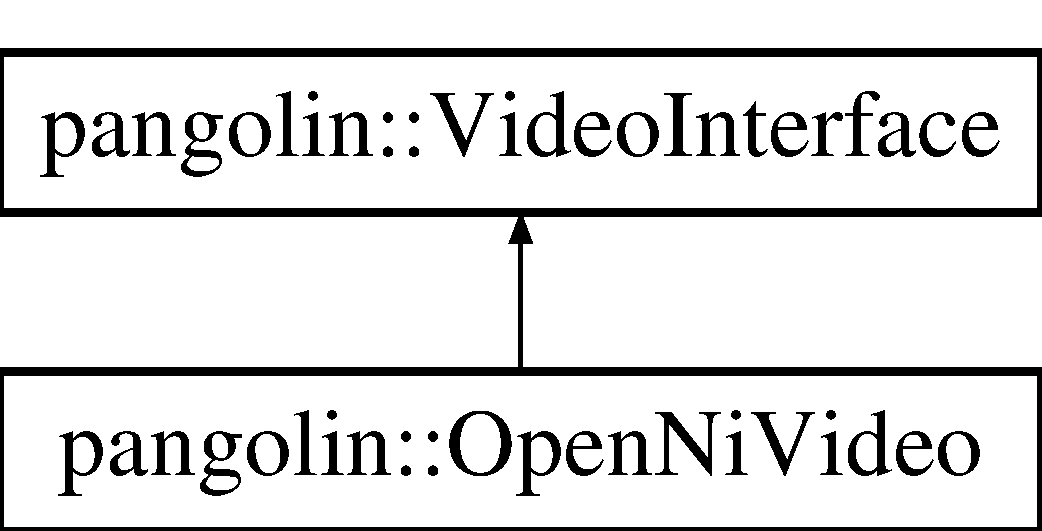
\includegraphics[height=2.000000cm]{structpangolin_1_1_open_ni_video}
\end{center}
\end{figure}
\subsection*{Public Member Functions}
\begin{DoxyCompactItemize}
\item 
{\bfseries Open\+Ni\+Video} (Open\+Ni\+Sensor\+Type s1, Open\+Ni\+Sensor\+Type s2, \hyperlink{structpangolin_1_1_image_dim}{Image\+Dim} dim=\hyperlink{structpangolin_1_1_image_dim}{Image\+Dim}(640, 480), int fps=30)\hypertarget{structpangolin_1_1_open_ni_video_a6d93fba2bcd7dbe988d572eda98a47ab}{}\label{structpangolin_1_1_open_ni_video_a6d93fba2bcd7dbe988d572eda98a47ab}

\item 
void \hyperlink{structpangolin_1_1_open_ni_video_af77e72402c088527c11d663b2ebaee90}{Start} ()\hypertarget{structpangolin_1_1_open_ni_video_af77e72402c088527c11d663b2ebaee90}{}\label{structpangolin_1_1_open_ni_video_af77e72402c088527c11d663b2ebaee90}

\begin{DoxyCompactList}\small\item\em Implement \hyperlink{structpangolin_1_1_video_input_a74a2e3e1b87c7cbf9de9bcb39e1df128}{Video\+Input\+::\+Start()} \end{DoxyCompactList}\item 
void \hyperlink{structpangolin_1_1_open_ni_video_a8435ecba39ae1d7b9372580a68be8a51}{Stop} ()\hypertarget{structpangolin_1_1_open_ni_video_a8435ecba39ae1d7b9372580a68be8a51}{}\label{structpangolin_1_1_open_ni_video_a8435ecba39ae1d7b9372580a68be8a51}

\begin{DoxyCompactList}\small\item\em Implement \hyperlink{structpangolin_1_1_video_input_a8945f80194cc7ec9594db7f27e7d09b8}{Video\+Input\+::\+Stop()} \end{DoxyCompactList}\item 
size\+\_\+t \hyperlink{structpangolin_1_1_open_ni_video_ad58408c831e7e1ed900dc99dcd4b9cf7}{Size\+Bytes} () const \hypertarget{structpangolin_1_1_open_ni_video_ad58408c831e7e1ed900dc99dcd4b9cf7}{}\label{structpangolin_1_1_open_ni_video_ad58408c831e7e1ed900dc99dcd4b9cf7}

\begin{DoxyCompactList}\small\item\em Implement \hyperlink{structpangolin_1_1_video_input_a93cee5c33386973a2a51165e6bdcf40b}{Video\+Input\+::\+Size\+Bytes()} \end{DoxyCompactList}\item 
const std\+::vector$<$ \hyperlink{classpangolin_1_1_stream_info}{Stream\+Info} $>$ \& \hyperlink{structpangolin_1_1_open_ni_video_a8084e7beefb248703b1667a4d940d8b4}{Streams} () const \hypertarget{structpangolin_1_1_open_ni_video_a8084e7beefb248703b1667a4d940d8b4}{}\label{structpangolin_1_1_open_ni_video_a8084e7beefb248703b1667a4d940d8b4}

\begin{DoxyCompactList}\small\item\em Implement \hyperlink{structpangolin_1_1_video_input_a9030d775d699c39ab7b7ba378c007c6a}{Video\+Input\+::\+Streams()} \end{DoxyCompactList}\item 
bool \hyperlink{structpangolin_1_1_open_ni_video_aa83894708b9410b457b9dcf5a4e05b5e}{Grab\+Next} (unsigned char $\ast$image, bool wait=true)\hypertarget{structpangolin_1_1_open_ni_video_aa83894708b9410b457b9dcf5a4e05b5e}{}\label{structpangolin_1_1_open_ni_video_aa83894708b9410b457b9dcf5a4e05b5e}

\begin{DoxyCompactList}\small\item\em Implement \hyperlink{structpangolin_1_1_video_input_ad3d8ff59c1ec4139320097e6e1111f32}{Video\+Input\+::\+Grab\+Next()} \end{DoxyCompactList}\item 
bool \hyperlink{structpangolin_1_1_open_ni_video_af98e477d47faffc3ca5389acb1d7f1ca}{Grab\+Newest} (unsigned char $\ast$image, bool wait=true)\hypertarget{structpangolin_1_1_open_ni_video_af98e477d47faffc3ca5389acb1d7f1ca}{}\label{structpangolin_1_1_open_ni_video_af98e477d47faffc3ca5389acb1d7f1ca}

\begin{DoxyCompactList}\small\item\em Implement \hyperlink{structpangolin_1_1_video_input_a4c8ac38e3c6a3f591663aeebf645e4c6}{Video\+Input\+::\+Grab\+Newest()} \end{DoxyCompactList}\item 
void {\bfseries Set\+Auto\+Exposure} (bool enabled)\hypertarget{structpangolin_1_1_open_ni_video_a2ee4009ea3058beecc11a1da11652fc8}{}\label{structpangolin_1_1_open_ni_video_a2ee4009ea3058beecc11a1da11652fc8}

\end{DoxyCompactItemize}
\subsection*{Protected Attributes}
\begin{DoxyCompactItemize}
\item 
std\+::vector$<$ \hyperlink{classpangolin_1_1_stream_info}{Stream\+Info} $>$ {\bfseries streams}\hypertarget{structpangolin_1_1_open_ni_video_a546a3995e35460ee7fe01baf4cbb6624}{}\label{structpangolin_1_1_open_ni_video_a546a3995e35460ee7fe01baf4cbb6624}

\item 
Open\+Ni\+Sensor\+Type {\bfseries sensor\+\_\+type} \mbox{[}2\mbox{]}\hypertarget{structpangolin_1_1_open_ni_video_aa9c3e7cb9414cfe0b36dd4ea11a49d9a}{}\label{structpangolin_1_1_open_ni_video_aa9c3e7cb9414cfe0b36dd4ea11a49d9a}

\item 
xn\+::\+Context {\bfseries context}\hypertarget{structpangolin_1_1_open_ni_video_a393c80caa5ce7ff1b86de4b36778bdfc}{}\label{structpangolin_1_1_open_ni_video_a393c80caa5ce7ff1b86de4b36778bdfc}

\item 
xn\+::\+Depth\+Generator {\bfseries depth\+Node}\hypertarget{structpangolin_1_1_open_ni_video_a6d746cf4caba53b49dfd8076670faebc}{}\label{structpangolin_1_1_open_ni_video_a6d746cf4caba53b49dfd8076670faebc}

\item 
xn\+::\+Image\+Generator {\bfseries image\+Node}\hypertarget{structpangolin_1_1_open_ni_video_a9bc169dc6e7383c2b232ae3dca2abe6f}{}\label{structpangolin_1_1_open_ni_video_a9bc169dc6e7383c2b232ae3dca2abe6f}

\item 
xn\+::\+I\+R\+Generator {\bfseries ir\+Node}\hypertarget{structpangolin_1_1_open_ni_video_a906f8046e534c6a73545e04fc88bbd98}{}\label{structpangolin_1_1_open_ni_video_a906f8046e534c6a73545e04fc88bbd98}

\item 
size\+\_\+t {\bfseries size\+Bytes}\hypertarget{structpangolin_1_1_open_ni_video_a5a28e0dcf514daf69f4b92e47fff56a8}{}\label{structpangolin_1_1_open_ni_video_a5a28e0dcf514daf69f4b92e47fff56a8}

\end{DoxyCompactItemize}


\subsection{Detailed Description}
Interface to video capture sources. 

The documentation for this struct was generated from the following file\+:\begin{DoxyCompactItemize}
\item 
/home/gapo/meng/deps/pangolin/include/pangolin/video/drivers/openni.\+h\end{DoxyCompactItemize}

\hypertarget{structpangolin_1_1_open_ni_video2}{}\section{pangolin\+:\+:Open\+Ni\+Video2 Struct Reference}
\label{structpangolin_1_1_open_ni_video2}\index{pangolin\+::\+Open\+Ni\+Video2@{pangolin\+::\+Open\+Ni\+Video2}}


Interface to video capture sources.  




{\ttfamily \#include $<$openni2.\+h$>$}

Inheritance diagram for pangolin\+:\+:Open\+Ni\+Video2\+:\begin{figure}[H]
\begin{center}
\leavevmode
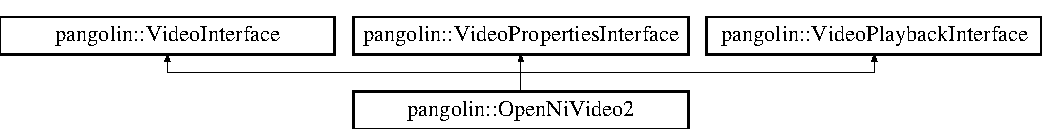
\includegraphics[height=1.736434cm]{structpangolin_1_1_open_ni_video2}
\end{center}
\end{figure}
\subsection*{Public Member Functions}
\begin{DoxyCompactItemize}
\item 
{\bfseries Open\+Ni\+Video2} (\hyperlink{structpangolin_1_1_image_dim}{Image\+Dim} dim=\hyperlink{structpangolin_1_1_image_dim}{Image\+Dim}(640, 480), int fps=30)\hypertarget{structpangolin_1_1_open_ni_video2_a3d7abca592256f39342a1e3c53d43683}{}\label{structpangolin_1_1_open_ni_video2_a3d7abca592256f39342a1e3c53d43683}

\item 
{\bfseries Open\+Ni\+Video2} (std\+::vector$<$ \hyperlink{structpangolin_1_1_open_ni_stream_mode}{Open\+Ni\+Stream\+Mode} $>$ \&stream\+\_\+modes)\hypertarget{structpangolin_1_1_open_ni_video2_a7bc1485077cb7829502a4af5cdd086d0}{}\label{structpangolin_1_1_open_ni_video2_a7bc1485077cb7829502a4af5cdd086d0}

\item 
{\bfseries Open\+Ni\+Video2} (const std\+::string \&filename)\hypertarget{structpangolin_1_1_open_ni_video2_a82f65ee9cad3e7954e40319872110e57}{}\label{structpangolin_1_1_open_ni_video2_a82f65ee9cad3e7954e40319872110e57}

\item 
{\bfseries Open\+Ni\+Video2} (const std\+::string \&filename, std\+::vector$<$ \hyperlink{structpangolin_1_1_open_ni_stream_mode}{Open\+Ni\+Stream\+Mode} $>$ \&stream\+\_\+modes)\hypertarget{structpangolin_1_1_open_ni_video2_a4d6a941bd0e3f380f9071ae2e5fdd32d}{}\label{structpangolin_1_1_open_ni_video2_a4d6a941bd0e3f380f9071ae2e5fdd32d}

\item 
void {\bfseries Update\+Properties} ()\hypertarget{structpangolin_1_1_open_ni_video2_a9ba2c0fa25ae7fef7556c4e27de11275}{}\label{structpangolin_1_1_open_ni_video2_a9ba2c0fa25ae7fef7556c4e27de11275}

\item 
void {\bfseries Set\+Mirroring} (bool enable)\hypertarget{structpangolin_1_1_open_ni_video2_a7804a6a59a5b1357eaa4ceb08d419fdb}{}\label{structpangolin_1_1_open_ni_video2_a7804a6a59a5b1357eaa4ceb08d419fdb}

\item 
void {\bfseries Set\+Auto\+Exposure} (bool enable)\hypertarget{structpangolin_1_1_open_ni_video2_a604c1bb67b1e9038bac2a8a3f6ed6f14}{}\label{structpangolin_1_1_open_ni_video2_a604c1bb67b1e9038bac2a8a3f6ed6f14}

\item 
void {\bfseries Set\+Auto\+White\+Balance} (bool enable)\hypertarget{structpangolin_1_1_open_ni_video2_a822da9d76b3980ae84136ea847ab0223}{}\label{structpangolin_1_1_open_ni_video2_a822da9d76b3980ae84136ea847ab0223}

\item 
void {\bfseries Set\+Depth\+Close\+Range} (bool enable)\hypertarget{structpangolin_1_1_open_ni_video2_a289c3d75b83a234e2742d7413e6886ca}{}\label{structpangolin_1_1_open_ni_video2_a289c3d75b83a234e2742d7413e6886ca}

\item 
void {\bfseries Set\+Depth\+Hole\+Filter} (bool enable)\hypertarget{structpangolin_1_1_open_ni_video2_a79de574ac83ecd1c57c81bdddcdb9b82}{}\label{structpangolin_1_1_open_ni_video2_a79de574ac83ecd1c57c81bdddcdb9b82}

\item 
void {\bfseries Set\+Depth\+Color\+Sync\+Enabled} (bool enable)\hypertarget{structpangolin_1_1_open_ni_video2_aaad37de74c34822c9251a62aa3fcbadb}{}\label{structpangolin_1_1_open_ni_video2_aaad37de74c34822c9251a62aa3fcbadb}

\item 
void {\bfseries Set\+Register\+Depth\+To\+Image} (bool enable)\hypertarget{structpangolin_1_1_open_ni_video2_a45436e167e2a5a34e18e6832b5b08d64}{}\label{structpangolin_1_1_open_ni_video2_a45436e167e2a5a34e18e6832b5b08d64}

\item 
void {\bfseries Set\+Playback\+Speed} (float speed)\hypertarget{structpangolin_1_1_open_ni_video2_a9902c927e2e0b861fb2c8ba82a37d26d}{}\label{structpangolin_1_1_open_ni_video2_a9902c927e2e0b861fb2c8ba82a37d26d}

\item 
void {\bfseries Set\+Playback\+Repeat} (bool enabled)\hypertarget{structpangolin_1_1_open_ni_video2_a5fbab99ea4db12a187f09c888e20a14c}{}\label{structpangolin_1_1_open_ni_video2_a5fbab99ea4db12a187f09c888e20a14c}

\item 
void \hyperlink{structpangolin_1_1_open_ni_video2_ad96cffd4d819c62cda2dfefd41d4ef64}{Start} ()\hypertarget{structpangolin_1_1_open_ni_video2_ad96cffd4d819c62cda2dfefd41d4ef64}{}\label{structpangolin_1_1_open_ni_video2_ad96cffd4d819c62cda2dfefd41d4ef64}

\begin{DoxyCompactList}\small\item\em Implement \hyperlink{structpangolin_1_1_video_input_a74a2e3e1b87c7cbf9de9bcb39e1df128}{Video\+Input\+::\+Start()} \end{DoxyCompactList}\item 
void \hyperlink{structpangolin_1_1_open_ni_video2_a482cf145fc2287a75a4946aff8723ff9}{Stop} ()\hypertarget{structpangolin_1_1_open_ni_video2_a482cf145fc2287a75a4946aff8723ff9}{}\label{structpangolin_1_1_open_ni_video2_a482cf145fc2287a75a4946aff8723ff9}

\begin{DoxyCompactList}\small\item\em Implement \hyperlink{structpangolin_1_1_video_input_a8945f80194cc7ec9594db7f27e7d09b8}{Video\+Input\+::\+Stop()} \end{DoxyCompactList}\item 
size\+\_\+t \hyperlink{structpangolin_1_1_open_ni_video2_ade76fea434e9107d161448a9a0d213cf}{Size\+Bytes} () const \hypertarget{structpangolin_1_1_open_ni_video2_ade76fea434e9107d161448a9a0d213cf}{}\label{structpangolin_1_1_open_ni_video2_ade76fea434e9107d161448a9a0d213cf}

\begin{DoxyCompactList}\small\item\em Implement \hyperlink{structpangolin_1_1_video_input_a93cee5c33386973a2a51165e6bdcf40b}{Video\+Input\+::\+Size\+Bytes()} \end{DoxyCompactList}\item 
const std\+::vector$<$ \hyperlink{classpangolin_1_1_stream_info}{Stream\+Info} $>$ \& \hyperlink{structpangolin_1_1_open_ni_video2_ade75fdf5fa9386482c97884eadddf8ed}{Streams} () const \hypertarget{structpangolin_1_1_open_ni_video2_ade75fdf5fa9386482c97884eadddf8ed}{}\label{structpangolin_1_1_open_ni_video2_ade75fdf5fa9386482c97884eadddf8ed}

\begin{DoxyCompactList}\small\item\em Implement \hyperlink{structpangolin_1_1_video_input_a9030d775d699c39ab7b7ba378c007c6a}{Video\+Input\+::\+Streams()} \end{DoxyCompactList}\item 
bool \hyperlink{structpangolin_1_1_open_ni_video2_ad9708e8f0096411d62e9babedc4c540e}{Grab\+Next} (unsigned char $\ast$image, bool wait=true)\hypertarget{structpangolin_1_1_open_ni_video2_ad9708e8f0096411d62e9babedc4c540e}{}\label{structpangolin_1_1_open_ni_video2_ad9708e8f0096411d62e9babedc4c540e}

\begin{DoxyCompactList}\small\item\em Implement \hyperlink{structpangolin_1_1_video_input_ad3d8ff59c1ec4139320097e6e1111f32}{Video\+Input\+::\+Grab\+Next()} \end{DoxyCompactList}\item 
bool \hyperlink{structpangolin_1_1_open_ni_video2_a13a3b106b6fad2d29cb9f5d0418115bd}{Grab\+Newest} (unsigned char $\ast$image, bool wait=true)\hypertarget{structpangolin_1_1_open_ni_video2_a13a3b106b6fad2d29cb9f5d0418115bd}{}\label{structpangolin_1_1_open_ni_video2_a13a3b106b6fad2d29cb9f5d0418115bd}

\begin{DoxyCompactList}\small\item\em Implement \hyperlink{structpangolin_1_1_video_input_a4c8ac38e3c6a3f591663aeebf645e4c6}{Video\+Input\+::\+Grab\+Newest()} \end{DoxyCompactList}\item 
const \hyperlink{classpangolin_1_1json_1_1value}{json\+::value} \& \hyperlink{structpangolin_1_1_open_ni_video2_a88ecc482f4fa4fd8fe968767d8599dfe}{Device\+Properties} () const \hypertarget{structpangolin_1_1_open_ni_video2_a88ecc482f4fa4fd8fe968767d8599dfe}{}\label{structpangolin_1_1_open_ni_video2_a88ecc482f4fa4fd8fe968767d8599dfe}

\begin{DoxyCompactList}\small\item\em Implement Video\+Properties\+Interface\+::\+Properties() \end{DoxyCompactList}\item 
const \hyperlink{classpangolin_1_1json_1_1value}{json\+::value} \& \hyperlink{structpangolin_1_1_open_ni_video2_a48e8313868d35a98cb9284326db819c4}{Frame\+Properties} () const \hypertarget{structpangolin_1_1_open_ni_video2_a48e8313868d35a98cb9284326db819c4}{}\label{structpangolin_1_1_open_ni_video2_a48e8313868d35a98cb9284326db819c4}

\begin{DoxyCompactList}\small\item\em Implement Video\+Properties\+Interface\+::\+Properties() \end{DoxyCompactList}\item 
int \hyperlink{structpangolin_1_1_open_ni_video2_a2598632ccd7f5139e0ef2f57acd3717c}{Get\+Current\+Frame\+Id} () const \hypertarget{structpangolin_1_1_open_ni_video2_a2598632ccd7f5139e0ef2f57acd3717c}{}\label{structpangolin_1_1_open_ni_video2_a2598632ccd7f5139e0ef2f57acd3717c}

\begin{DoxyCompactList}\small\item\em Implement \hyperlink{structpangolin_1_1_video_playback_interface_a1853ad8ca4b10b8a87599d0c288b9c86}{Video\+Playback\+Interface\+::\+Get\+Current\+Frame\+Id}. \end{DoxyCompactList}\item 
int \hyperlink{structpangolin_1_1_open_ni_video2_ae36b50354e352f5faf7e396e35ba62d1}{Get\+Total\+Frames} () const \hypertarget{structpangolin_1_1_open_ni_video2_ae36b50354e352f5faf7e396e35ba62d1}{}\label{structpangolin_1_1_open_ni_video2_ae36b50354e352f5faf7e396e35ba62d1}

\begin{DoxyCompactList}\small\item\em Implement \hyperlink{structpangolin_1_1_video_playback_interface_aa1ab605b49009c52a80eaa0cc074b63b}{Video\+Playback\+Interface\+::\+Get\+Total\+Frames}. \end{DoxyCompactList}\item 
int \hyperlink{structpangolin_1_1_open_ni_video2_a5e6adf855444e787965943a582cef52a}{Seek} (int frameid)\hypertarget{structpangolin_1_1_open_ni_video2_a5e6adf855444e787965943a582cef52a}{}\label{structpangolin_1_1_open_ni_video2_a5e6adf855444e787965943a582cef52a}

\begin{DoxyCompactList}\small\item\em Implement \hyperlink{structpangolin_1_1_video_playback_interface_a0f65ae246e93ddc884b139ac0ba06d25}{Video\+Playback\+Interface\+::\+Seek}. \end{DoxyCompactList}\item 
openni\+::\+Video\+Stream $\ast$ {\bfseries Get\+Video\+Stream} (int stream)\hypertarget{structpangolin_1_1_open_ni_video2_acdddb6f2e9dd8fe2aaa2f3e3dc9adb22}{}\label{structpangolin_1_1_open_ni_video2_acdddb6f2e9dd8fe2aaa2f3e3dc9adb22}

\end{DoxyCompactItemize}
\subsection*{Protected Member Functions}
\begin{DoxyCompactItemize}
\item 
void {\bfseries Initialise\+Open\+NI} ()\hypertarget{structpangolin_1_1_open_ni_video2_a337acc14504a05184102a6f2147056e8}{}\label{structpangolin_1_1_open_ni_video2_a337acc14504a05184102a6f2147056e8}

\item 
int {\bfseries Add\+Device} (const std\+::string \&device\+\_\+uri)\hypertarget{structpangolin_1_1_open_ni_video2_a38c259b039428f1ce731530c26ed7881}{}\label{structpangolin_1_1_open_ni_video2_a38c259b039428f1ce731530c26ed7881}

\item 
void {\bfseries Add\+Stream} (const \hyperlink{structpangolin_1_1_open_ni_stream_mode}{Open\+Ni\+Stream\+Mode} \&mode)\hypertarget{structpangolin_1_1_open_ni_video2_a6f66deacc496313dbdf3d955dea72926}{}\label{structpangolin_1_1_open_ni_video2_a6f66deacc496313dbdf3d955dea72926}

\item 
void {\bfseries Setup\+Stream\+Modes} ()\hypertarget{structpangolin_1_1_open_ni_video2_a193e783e16265b14ddc71efb2297a201}{}\label{structpangolin_1_1_open_ni_video2_a193e783e16265b14ddc71efb2297a201}

\item 
void {\bfseries Print\+Open\+N\+I2\+Modes} (openni\+::\+Sensor\+Type sensor\+Type)\hypertarget{structpangolin_1_1_open_ni_video2_aaa42b62c37ec2ecd7d0cf3d05f579547}{}\label{structpangolin_1_1_open_ni_video2_aaa42b62c37ec2ecd7d0cf3d05f579547}

\item 
openni\+::\+Video\+Mode {\bfseries Find\+Open\+N\+I2\+Mode} (openni\+::\+Device \&device, openni\+::\+Sensor\+Type sensor\+Type, int width, int height, int fps, openni\+::\+Pixel\+Format fmt)\hypertarget{structpangolin_1_1_open_ni_video2_a57eabf23de55db37748c2050c09a21f7}{}\label{structpangolin_1_1_open_ni_video2_a57eabf23de55db37748c2050c09a21f7}

\end{DoxyCompactItemize}
\subsection*{Protected Attributes}
\begin{DoxyCompactItemize}
\item 
int {\bfseries num\+Devices}\hypertarget{structpangolin_1_1_open_ni_video2_a591547a69e59f7021fdf6088d3795f72}{}\label{structpangolin_1_1_open_ni_video2_a591547a69e59f7021fdf6088d3795f72}

\item 
int {\bfseries num\+Streams}\hypertarget{structpangolin_1_1_open_ni_video2_a2c8b3b00243e87c0fdfd3d83f47e267f}{}\label{structpangolin_1_1_open_ni_video2_a2c8b3b00243e87c0fdfd3d83f47e267f}

\item 
openni\+::\+Device {\bfseries devices} \mbox{[}O\+N\+I\+\_\+\+M\+A\+X\+\_\+\+S\+E\+N\+S\+O\+RS\mbox{]}\hypertarget{structpangolin_1_1_open_ni_video2_abe4d77667a3a14ee506cad7c52883f0e}{}\label{structpangolin_1_1_open_ni_video2_abe4d77667a3a14ee506cad7c52883f0e}

\item 
\hyperlink{structpangolin_1_1_open_ni_stream_mode}{Open\+Ni\+Stream\+Mode} {\bfseries sensor\+\_\+type} \mbox{[}O\+N\+I\+\_\+\+M\+A\+X\+\_\+\+S\+E\+N\+S\+O\+RS\mbox{]}\hypertarget{structpangolin_1_1_open_ni_video2_a3e97f9399e40bc2f291bdb6272a21368}{}\label{structpangolin_1_1_open_ni_video2_a3e97f9399e40bc2f291bdb6272a21368}

\item 
openni\+::\+Video\+Stream {\bfseries video\+\_\+stream} \mbox{[}O\+N\+I\+\_\+\+M\+A\+X\+\_\+\+S\+E\+N\+S\+O\+RS\mbox{]}\hypertarget{structpangolin_1_1_open_ni_video2_a88808fe1e6b593f452cb1bc567c80209}{}\label{structpangolin_1_1_open_ni_video2_a88808fe1e6b593f452cb1bc567c80209}

\item 
openni\+::\+Video\+Frame\+Ref {\bfseries video\+\_\+frame} \mbox{[}O\+N\+I\+\_\+\+M\+A\+X\+\_\+\+S\+E\+N\+S\+O\+RS\mbox{]}\hypertarget{structpangolin_1_1_open_ni_video2_a3dbfeeb2cd27f814fea8468b2bc5fcef}{}\label{structpangolin_1_1_open_ni_video2_a3dbfeeb2cd27f814fea8468b2bc5fcef}

\item 
std\+::vector$<$ \hyperlink{classpangolin_1_1_stream_info}{Stream\+Info} $>$ {\bfseries streams}\hypertarget{structpangolin_1_1_open_ni_video2_a3d3ec9bf9379c7e9520a32853a6c37cc}{}\label{structpangolin_1_1_open_ni_video2_a3d3ec9bf9379c7e9520a32853a6c37cc}

\item 
size\+\_\+t {\bfseries size\+Bytes}\hypertarget{structpangolin_1_1_open_ni_video2_a74ce33e834d7fdd7f94fa70390bd763b}{}\label{structpangolin_1_1_open_ni_video2_a74ce33e834d7fdd7f94fa70390bd763b}

\item 
\hyperlink{classpangolin_1_1json_1_1value}{json\+::value} {\bfseries device\+\_\+properties}\hypertarget{structpangolin_1_1_open_ni_video2_a71d024658a693c313803164a9cf35510}{}\label{structpangolin_1_1_open_ni_video2_a71d024658a693c313803164a9cf35510}

\item 
\hyperlink{classpangolin_1_1json_1_1value}{json\+::value} {\bfseries frame\+\_\+properties}\hypertarget{structpangolin_1_1_open_ni_video2_a20f4db05b50835b24a76ddf2156b658d}{}\label{structpangolin_1_1_open_ni_video2_a20f4db05b50835b24a76ddf2156b658d}

\item 
\hyperlink{classpangolin_1_1json_1_1value}{json\+::value} $\ast$ {\bfseries streams\+\_\+properties}\hypertarget{structpangolin_1_1_open_ni_video2_ae16067ea064d0fc249128371e092a92c}{}\label{structpangolin_1_1_open_ni_video2_ae16067ea064d0fc249128371e092a92c}

\item 
bool {\bfseries use\+\_\+depth}\hypertarget{structpangolin_1_1_open_ni_video2_a8cedd9f800257bae6307b244d2d4f125}{}\label{structpangolin_1_1_open_ni_video2_a8cedd9f800257bae6307b244d2d4f125}

\item 
bool {\bfseries use\+\_\+ir}\hypertarget{structpangolin_1_1_open_ni_video2_a5e5d76e55e1d42d377026dc6d54326e6}{}\label{structpangolin_1_1_open_ni_video2_a5e5d76e55e1d42d377026dc6d54326e6}

\item 
bool {\bfseries use\+\_\+rgb}\hypertarget{structpangolin_1_1_open_ni_video2_a639683069b9b39c75c2e31856a34fca6}{}\label{structpangolin_1_1_open_ni_video2_a639683069b9b39c75c2e31856a34fca6}

\item 
bool {\bfseries depth\+\_\+to\+\_\+color}\hypertarget{structpangolin_1_1_open_ni_video2_abfee91ae56ee3b99b214af8fb8a3a239}{}\label{structpangolin_1_1_open_ni_video2_abfee91ae56ee3b99b214af8fb8a3a239}

\item 
bool {\bfseries use\+\_\+ir\+\_\+and\+\_\+rgb}\hypertarget{structpangolin_1_1_open_ni_video2_afb57bb26f834c7c0f710e472c374adcb}{}\label{structpangolin_1_1_open_ni_video2_afb57bb26f834c7c0f710e472c374adcb}

\item 
bool {\bfseries from\+File}\hypertarget{structpangolin_1_1_open_ni_video2_ab26a4c783672fe293bc07211d05fc25b}{}\label{structpangolin_1_1_open_ni_video2_ab26a4c783672fe293bc07211d05fc25b}

\item 
int {\bfseries current\+\_\+frame\+\_\+index}\hypertarget{structpangolin_1_1_open_ni_video2_a1abbc73d4b9dceea8ceeaa6657f1e471}{}\label{structpangolin_1_1_open_ni_video2_a1abbc73d4b9dceea8ceeaa6657f1e471}

\item 
int {\bfseries total\+\_\+frames}\hypertarget{structpangolin_1_1_open_ni_video2_a77ba8f227738d995ded204b8b14704c5}{}\label{structpangolin_1_1_open_ni_video2_a77ba8f227738d995ded204b8b14704c5}

\end{DoxyCompactItemize}


\subsection{Detailed Description}
Interface to video capture sources. 

The documentation for this struct was generated from the following file\+:\begin{DoxyCompactItemize}
\item 
/home/gapo/meng/deps/pangolin/include/pangolin/video/drivers/openni2.\+h\end{DoxyCompactItemize}

\hypertarget{classpangolin_1_1_packet_stream_reader}{}\section{pangolin\+:\+:Packet\+Stream\+Reader Class Reference}
\label{classpangolin_1_1_packet_stream_reader}\index{pangolin\+::\+Packet\+Stream\+Reader@{pangolin\+::\+Packet\+Stream\+Reader}}
\subsection*{Public Member Functions}
\begin{DoxyCompactItemize}
\item 
{\bfseries Packet\+Stream\+Reader} (const std\+::string \&filename, bool realtime=true)\hypertarget{classpangolin_1_1_packet_stream_reader_a23167792afe67996054ba235d4037b3f}{}\label{classpangolin_1_1_packet_stream_reader_a23167792afe67996054ba235d4037b3f}

\item 
void {\bfseries Open} (const std\+::string \&filename, bool realtime=true)\hypertarget{classpangolin_1_1_packet_stream_reader_a1b331c0e8749b20e22d474d9a36f5eb3}{}\label{classpangolin_1_1_packet_stream_reader_a1b331c0e8749b20e22d474d9a36f5eb3}

\item 
void {\bfseries Close} ()\hypertarget{classpangolin_1_1_packet_stream_reader_a9779adccfba39d9284bbc0f2463a833e}{}\label{classpangolin_1_1_packet_stream_reader_a9779adccfba39d9284bbc0f2463a833e}

\item 
const std\+::vector$<$ \hyperlink{structpangolin_1_1_packet_stream_source}{Packet\+Stream\+Source} $>$ \& {\bfseries Sources} () const \hypertarget{classpangolin_1_1_packet_stream_reader_a44524078dc65d6eb3ac5af77f95ebe7e}{}\label{classpangolin_1_1_packet_stream_reader_a44524078dc65d6eb3ac5af77f95ebe7e}

\item 
bool {\bfseries Read\+To\+Source\+Packet\+And\+Lock} (Packet\+Stream\+Source\+Id src\+\_\+id)\hypertarget{classpangolin_1_1_packet_stream_reader_a4973f580b31d4fead776e58323338c31}{}\label{classpangolin_1_1_packet_stream_reader_a4973f580b31d4fead776e58323338c31}

\item 
void {\bfseries Release\+Source\+Packet\+Lock} (Packet\+Stream\+Source\+Id src\+\_\+id)\hypertarget{classpangolin_1_1_packet_stream_reader_af4cc1d531c2dcb229103e9e99994486e}{}\label{classpangolin_1_1_packet_stream_reader_af4cc1d531c2dcb229103e9e99994486e}

\item 
std\+::basic\+\_\+istream$<$ char $>$ \& {\bfseries Read} (char $\ast$s, size\+\_\+t n)\hypertarget{classpangolin_1_1_packet_stream_reader_a03aec2d97f5c5af53d0d09cbb7f5377d}{}\label{classpangolin_1_1_packet_stream_reader_a03aec2d97f5c5af53d0d09cbb7f5377d}

\end{DoxyCompactItemize}
\subsection*{Protected Member Functions}
\begin{DoxyCompactItemize}
\item 
int64\+\_\+t {\bfseries Read\+Timestamp} ()\hypertarget{classpangolin_1_1_packet_stream_reader_aadca1f14ec7e421831e3b0a4b34c1f45}{}\label{classpangolin_1_1_packet_stream_reader_aadca1f14ec7e421831e3b0a4b34c1f45}

\item 
size\+\_\+t {\bfseries Read\+Compressed\+Unsigned\+Int} ()\hypertarget{classpangolin_1_1_packet_stream_reader_ac594ef5afa759ce58b3ae2a2fc0a3420}{}\label{classpangolin_1_1_packet_stream_reader_ac594ef5afa759ce58b3ae2a2fc0a3420}

\item 
void {\bfseries Process\+Message} ()\hypertarget{classpangolin_1_1_packet_stream_reader_a090d547ec84af0003dfe5d43f2f01e9f}{}\label{classpangolin_1_1_packet_stream_reader_a090d547ec84af0003dfe5d43f2f01e9f}

\item 
void {\bfseries Process\+Messages\+Until\+Source\+Packet} (int \&nxt\+\_\+src\+\_\+id, int64\+\_\+t \&time\+\_\+us)\hypertarget{classpangolin_1_1_packet_stream_reader_a421f6924b19826ac412822d2d54f56e6}{}\label{classpangolin_1_1_packet_stream_reader_a421f6924b19826ac412822d2d54f56e6}

\item 
bool {\bfseries Read\+Tag} ()\hypertarget{classpangolin_1_1_packet_stream_reader_acc53cd09b91d94629c44c189f42b942e}{}\label{classpangolin_1_1_packet_stream_reader_acc53cd09b91d94629c44c189f42b942e}

\item 
void {\bfseries Read\+Header\+Packet} ()\hypertarget{classpangolin_1_1_packet_stream_reader_aa7756bbe7d074c8fc6ff18124f069d8a}{}\label{classpangolin_1_1_packet_stream_reader_aa7756bbe7d074c8fc6ff18124f069d8a}

\item 
void {\bfseries Read\+Source\+Packet\+Meta} (\hyperlink{classpangolin_1_1json_1_1value}{json\+::value} \&json)\hypertarget{classpangolin_1_1_packet_stream_reader_a3ba94740c0f9a43e1e2750f5271536bd}{}\label{classpangolin_1_1_packet_stream_reader_a3ba94740c0f9a43e1e2750f5271536bd}

\item 
void {\bfseries Read\+New\+Source\+Packet} ()\hypertarget{classpangolin_1_1_packet_stream_reader_a84ec5d9535eea4a0fabedb00fa15140e}{}\label{classpangolin_1_1_packet_stream_reader_a84ec5d9535eea4a0fabedb00fa15140e}

\item 
void {\bfseries Read\+Stats\+Packet} ()\hypertarget{classpangolin_1_1_packet_stream_reader_ad0a465df200d79caba45efc373f30d34}{}\label{classpangolin_1_1_packet_stream_reader_ad0a465df200d79caba45efc373f30d34}

\item 
void {\bfseries Read\+Over\+Source\+Packet} (Packet\+Stream\+Source\+Id src\+\_\+id)\hypertarget{classpangolin_1_1_packet_stream_reader_af5ac5ea1d39fdf07529d474c065b350b}{}\label{classpangolin_1_1_packet_stream_reader_af5ac5ea1d39fdf07529d474c065b350b}

\end{DoxyCompactItemize}
\subsection*{Protected Attributes}
\begin{DoxyCompactItemize}
\item 
uint32\+\_\+t {\bfseries next\+\_\+tag}\hypertarget{classpangolin_1_1_packet_stream_reader_a7239d69f9b43fac490395bcbce28c134}{}\label{classpangolin_1_1_packet_stream_reader_a7239d69f9b43fac490395bcbce28c134}

\item 
std\+::vector$<$ \hyperlink{structpangolin_1_1_packet_stream_source}{Packet\+Stream\+Source} $>$ {\bfseries sources}\hypertarget{classpangolin_1_1_packet_stream_reader_ae3898701de5378a9915e4227ffca0378}{}\label{classpangolin_1_1_packet_stream_reader_ae3898701de5378a9915e4227ffca0378}

\item 
std\+::ifstream {\bfseries reader}\hypertarget{classpangolin_1_1_packet_stream_reader_a0972aad6e76f5b2ff52da1cedb9fc652}{}\label{classpangolin_1_1_packet_stream_reader_a0972aad6e76f5b2ff52da1cedb9fc652}

\item 
boostd\+::mutex {\bfseries read\+\_\+mutex}\hypertarget{classpangolin_1_1_packet_stream_reader_aef1a3ce851522a0778a5af396dd150ce}{}\label{classpangolin_1_1_packet_stream_reader_aef1a3ce851522a0778a5af396dd150ce}

\item 
int {\bfseries packets}\hypertarget{classpangolin_1_1_packet_stream_reader_acbb565d521eaf0fe3165b747c85c478f}{}\label{classpangolin_1_1_packet_stream_reader_acbb565d521eaf0fe3165b747c85c478f}

\item 
bool {\bfseries realtime}\hypertarget{classpangolin_1_1_packet_stream_reader_a13dbb3164ace61d512eeb7a3980624c3}{}\label{classpangolin_1_1_packet_stream_reader_a13dbb3164ace61d512eeb7a3980624c3}

\end{DoxyCompactItemize}


The documentation for this class was generated from the following file\+:\begin{DoxyCompactItemize}
\item 
/home/gapo/meng/deps/pangolin/include/pangolin/log/packetstream.\+h\end{DoxyCompactItemize}

\hypertarget{structpangolin_1_1_packet_stream_source}{}\section{pangolin\+:\+:Packet\+Stream\+Source Struct Reference}
\label{structpangolin_1_1_packet_stream_source}\index{pangolin\+::\+Packet\+Stream\+Source@{pangolin\+::\+Packet\+Stream\+Source}}
\subsection*{Public Attributes}
\begin{DoxyCompactItemize}
\item 
std\+::string {\bfseries driver}\hypertarget{structpangolin_1_1_packet_stream_source_aaec90bc5f35a4fbacc2fb0ee4a8ea7e9}{}\label{structpangolin_1_1_packet_stream_source_aaec90bc5f35a4fbacc2fb0ee4a8ea7e9}

\item 
int {\bfseries id}\hypertarget{structpangolin_1_1_packet_stream_source_a67bda15da2041ed87748985db150792e}{}\label{structpangolin_1_1_packet_stream_source_a67bda15da2041ed87748985db150792e}

\item 
std\+::string {\bfseries uri}\hypertarget{structpangolin_1_1_packet_stream_source_ab767606ce98e4bfbc9f3f45eca36ae56}{}\label{structpangolin_1_1_packet_stream_source_ab767606ce98e4bfbc9f3f45eca36ae56}

\item 
\hyperlink{classpangolin_1_1json_1_1value}{json\+::value} {\bfseries info}\hypertarget{structpangolin_1_1_packet_stream_source_a7ca8ff4525ccc0888b522f7babc22e35}{}\label{structpangolin_1_1_packet_stream_source_a7ca8ff4525ccc0888b522f7babc22e35}

\item 
\hyperlink{classpangolin_1_1json_1_1value}{json\+::value} {\bfseries meta}\hypertarget{structpangolin_1_1_packet_stream_source_a5e98fe15917a51ee216e93dc0fb03267}{}\label{structpangolin_1_1_packet_stream_source_a5e98fe15917a51ee216e93dc0fb03267}

\item 
int64\+\_\+t {\bfseries version}\hypertarget{structpangolin_1_1_packet_stream_source_aa798c8c7f91f2e321a9df4a665d443ee}{}\label{structpangolin_1_1_packet_stream_source_aa798c8c7f91f2e321a9df4a665d443ee}

\item 
int64\+\_\+t {\bfseries data\+\_\+alignment\+\_\+bytes}\hypertarget{structpangolin_1_1_packet_stream_source_a68b8de8c48d952f23a94750fbe3bde9e}{}\label{structpangolin_1_1_packet_stream_source_a68b8de8c48d952f23a94750fbe3bde9e}

\item 
std\+::string {\bfseries data\+\_\+definitions}\hypertarget{structpangolin_1_1_packet_stream_source_ab1203cf37bab135465db99b0bdfd6be6}{}\label{structpangolin_1_1_packet_stream_source_ab1203cf37bab135465db99b0bdfd6be6}

\item 
int64\+\_\+t {\bfseries data\+\_\+size\+\_\+bytes}\hypertarget{structpangolin_1_1_packet_stream_source_a988591b8374aa1457766ae7202e8b9e6}{}\label{structpangolin_1_1_packet_stream_source_a988591b8374aa1457766ae7202e8b9e6}

\end{DoxyCompactItemize}


The documentation for this struct was generated from the following file\+:\begin{DoxyCompactItemize}
\item 
/home/gapo/meng/deps/pangolin/include/pangolin/log/packetstream.\+h\end{DoxyCompactItemize}

\hypertarget{classpangolin_1_1_packet_stream_writer}{}\section{pangolin\+:\+:Packet\+Stream\+Writer Class Reference}
\label{classpangolin_1_1_packet_stream_writer}\index{pangolin\+::\+Packet\+Stream\+Writer@{pangolin\+::\+Packet\+Stream\+Writer}}
\subsection*{Public Member Functions}
\begin{DoxyCompactItemize}
\item 
{\bfseries Packet\+Stream\+Writer} (const std\+::string \&filename, unsigned int buffer\+\_\+size\+\_\+bytes=10000000)\hypertarget{classpangolin_1_1_packet_stream_writer_aa157486194193ca4a8f68fb203637800}{}\label{classpangolin_1_1_packet_stream_writer_aa157486194193ca4a8f68fb203637800}

\item 
void {\bfseries Open} (const std\+::string \&filename, unsigned int buffer\+\_\+size\+\_\+bytes=10000000)\hypertarget{classpangolin_1_1_packet_stream_writer_aa514d5604ac0f347f7275c434f37bdca}{}\label{classpangolin_1_1_packet_stream_writer_aa514d5604ac0f347f7275c434f37bdca}

\item 
Packet\+Stream\+Source\+Id {\bfseries Add\+Source} (const std\+::string \&source\+\_\+driver, const std\+::string \&source\+\_\+uri, const \hyperlink{classpangolin_1_1json_1_1value}{json\+::value} \&json\+\_\+header=\hyperlink{classpangolin_1_1json_1_1value}{json\+::value}(), const size\+\_\+t packet\+\_\+size\+\_\+bytes=0, const std\+::string \&packet\+\_\+definitions=\char`\"{}\char`\"{})\hypertarget{classpangolin_1_1_packet_stream_writer_aff95a47df0697479f63a98d8021bb2c1}{}\label{classpangolin_1_1_packet_stream_writer_aff95a47df0697479f63a98d8021bb2c1}

\item 
void {\bfseries Write\+Source\+Packet\+Meta} (Packet\+Stream\+Source\+Id src, const \hyperlink{classpangolin_1_1json_1_1value}{json\+::value} \&json)\hypertarget{classpangolin_1_1_packet_stream_writer_ae0b8269bdc55d16722e27fcc2ab687b6}{}\label{classpangolin_1_1_packet_stream_writer_ae0b8269bdc55d16722e27fcc2ab687b6}

\item 
void {\bfseries Write\+Source\+Packet} (Packet\+Stream\+Source\+Id src, const char $\ast$data, size\+\_\+t n)\hypertarget{classpangolin_1_1_packet_stream_writer_a04471a882b3cf388fb15b96536972997}{}\label{classpangolin_1_1_packet_stream_writer_a04471a882b3cf388fb15b96536972997}

\item 
void {\bfseries Write\+Pango\+Header} ()\hypertarget{classpangolin_1_1_packet_stream_writer_a98769a090eb605689cc88e6a5c3052c2}{}\label{classpangolin_1_1_packet_stream_writer_a98769a090eb605689cc88e6a5c3052c2}

\item 
void {\bfseries Write\+Stats} ()\hypertarget{classpangolin_1_1_packet_stream_writer_a8e66e558ba56dbec5f20aee019f25a7a}{}\label{classpangolin_1_1_packet_stream_writer_a8e66e558ba56dbec5f20aee019f25a7a}

\item 
void {\bfseries Write\+Sync} ()\hypertarget{classpangolin_1_1_packet_stream_writer_ab41e3271bd3b5ca136cdff5477439740}{}\label{classpangolin_1_1_packet_stream_writer_ab41e3271bd3b5ca136cdff5477439740}

\end{DoxyCompactItemize}
\subsection*{Protected Member Functions}
\begin{DoxyCompactItemize}
\item 
void {\bfseries Write\+Compressed\+Unsigned\+Int} (size\+\_\+t n)\hypertarget{classpangolin_1_1_packet_stream_writer_accf4896829d689b05f8cd374c99c67cb}{}\label{classpangolin_1_1_packet_stream_writer_accf4896829d689b05f8cd374c99c67cb}

\item 
void {\bfseries Write\+Timestamp} ()\hypertarget{classpangolin_1_1_packet_stream_writer_a37862edcb8b743f50949ba50ca286b50}{}\label{classpangolin_1_1_packet_stream_writer_a37862edcb8b743f50949ba50ca286b50}

\item 
void {\bfseries Write\+Tag} (const uint32\+\_\+t tag)\hypertarget{classpangolin_1_1_packet_stream_writer_a73a33d797e6c03ff26032f8ab3e4d238}{}\label{classpangolin_1_1_packet_stream_writer_a73a33d797e6c03ff26032f8ab3e4d238}

\end{DoxyCompactItemize}
\subsection*{Protected Attributes}
\begin{DoxyCompactItemize}
\item 
std\+::vector$<$ \hyperlink{structpangolin_1_1_packet_stream_source}{Packet\+Stream\+Source} $>$ {\bfseries sources}\hypertarget{classpangolin_1_1_packet_stream_writer_a3865a3f75df0d38b8693a9492ac69285}{}\label{classpangolin_1_1_packet_stream_writer_a3865a3f75df0d38b8693a9492ac69285}

\item 
\hyperlink{classpangolin_1_1threadedfilebuf}{threadedfilebuf} {\bfseries buffer}\hypertarget{classpangolin_1_1_packet_stream_writer_adc2cdfb08279b9d1c8902885513cfd56}{}\label{classpangolin_1_1_packet_stream_writer_adc2cdfb08279b9d1c8902885513cfd56}

\item 
std\+::ostream {\bfseries writer}\hypertarget{classpangolin_1_1_packet_stream_writer_ae00f3814caaa4890d7eb2f19e77c0c97}{}\label{classpangolin_1_1_packet_stream_writer_ae00f3814caaa4890d7eb2f19e77c0c97}

\item 
unsigned int {\bfseries bytes\+\_\+written}\hypertarget{classpangolin_1_1_packet_stream_writer_a66cb0699dcdb321bb6b3e160b3dbba5c}{}\label{classpangolin_1_1_packet_stream_writer_a66cb0699dcdb321bb6b3e160b3dbba5c}

\end{DoxyCompactItemize}


The documentation for this class was generated from the following file\+:\begin{DoxyCompactItemize}
\item 
/home/gapo/meng/deps/pangolin/include/pangolin/log/packetstream.\+h\end{DoxyCompactItemize}

\hypertarget{structpangolin_1_1_panel}{}\section{pangolin\+:\+:Panel Struct Reference}
\label{structpangolin_1_1_panel}\index{pangolin\+::\+Panel@{pangolin\+::\+Panel}}
Inheritance diagram for pangolin\+:\+:Panel\+:\begin{figure}[H]
\begin{center}
\leavevmode
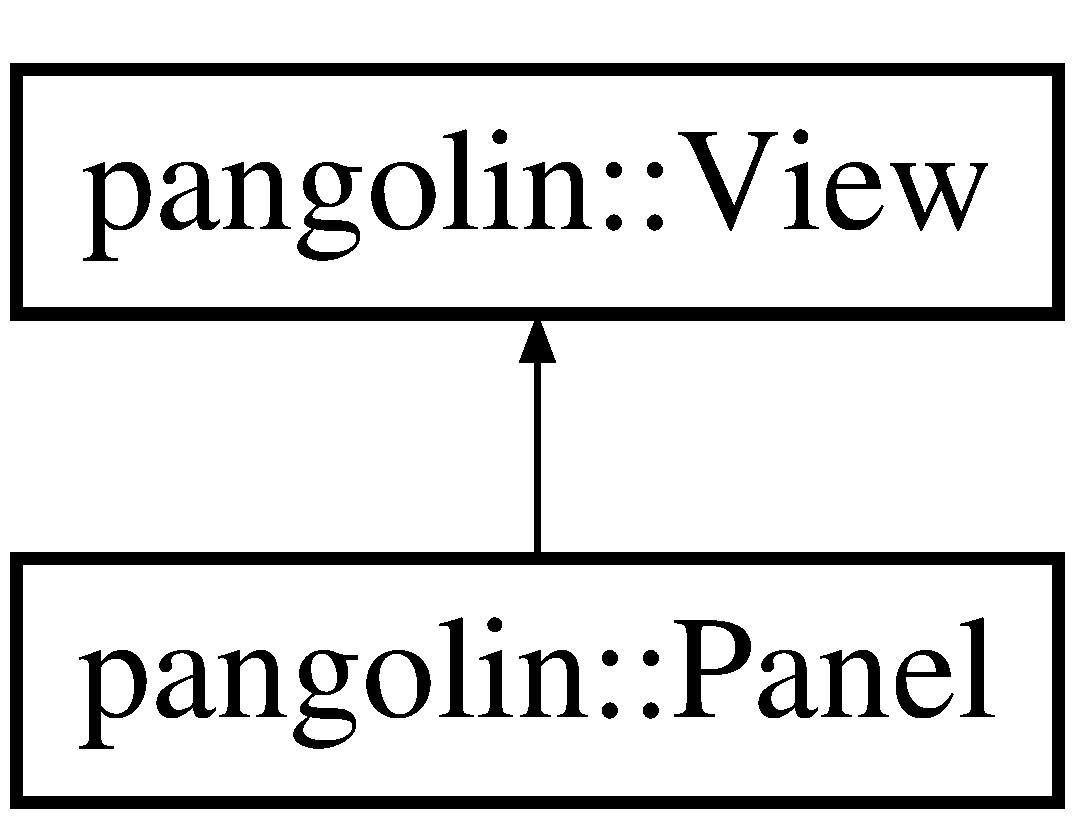
\includegraphics[height=2.000000cm]{structpangolin_1_1_panel}
\end{center}
\end{figure}
\subsection*{Public Member Functions}
\begin{DoxyCompactItemize}
\item 
{\bfseries Panel} (const std\+::string \&auto\+\_\+register\+\_\+var\+\_\+prefix)\hypertarget{structpangolin_1_1_panel_aa4def26e804158db784ce9720a2d7130}{}\label{structpangolin_1_1_panel_aa4def26e804158db784ce9720a2d7130}

\item 
void \hyperlink{structpangolin_1_1_panel_a4b9fa5d477bb518ad6917086d1faf2ca}{Render} ()
\begin{DoxyCompactList}\small\item\em Perform any automatic rendering for this \hyperlink{structpangolin_1_1_view}{View}. \end{DoxyCompactList}\item 
void \hyperlink{structpangolin_1_1_panel_aa7e3e26f6f45b2691755e055daf0317c}{Resize\+Children} ()\hypertarget{structpangolin_1_1_panel_aa7e3e26f6f45b2691755e055daf0317c}{}\label{structpangolin_1_1_panel_aa7e3e26f6f45b2691755e055daf0317c}

\begin{DoxyCompactList}\small\item\em Instruct all children to resize. \end{DoxyCompactList}\end{DoxyCompactItemize}
\subsection*{Static Public Member Functions}
\begin{DoxyCompactItemize}
\item 
static void {\bfseries Add\+Variable} (void $\ast$data, const std\+::string \&name, \hyperlink{classpangolin_1_1_var_value_generic}{Var\+Value\+Generic} \&var, bool brand\+\_\+new)\hypertarget{structpangolin_1_1_panel_a9b2b80fc8c13b4277d2d49d273251af3}{}\label{structpangolin_1_1_panel_a9b2b80fc8c13b4277d2d49d273251af3}

\end{DoxyCompactItemize}
\subsection*{Additional Inherited Members}


\subsection{Member Function Documentation}
\index{pangolin\+::\+Panel@{pangolin\+::\+Panel}!Render@{Render}}
\index{Render@{Render}!pangolin\+::\+Panel@{pangolin\+::\+Panel}}
\subsubsection[{\texorpdfstring{Render()}{Render()}}]{\setlength{\rightskip}{0pt plus 5cm}void pangolin\+::\+Panel\+::\+Render (
\begin{DoxyParamCaption}
{}
\end{DoxyParamCaption}
)\hspace{0.3cm}{\ttfamily [virtual]}}\hypertarget{structpangolin_1_1_panel_a4b9fa5d477bb518ad6917086d1faf2ca}{}\label{structpangolin_1_1_panel_a4b9fa5d477bb518ad6917086d1faf2ca}


Perform any automatic rendering for this \hyperlink{structpangolin_1_1_view}{View}. 

Default implementation simply instructs children to render themselves. 

Reimplemented from \hyperlink{structpangolin_1_1_view_a15bf43d7ebc4ebe4e02cba572f0d49ba}{pangolin\+::\+View}.



The documentation for this struct was generated from the following file\+:\begin{DoxyCompactItemize}
\item 
/home/gapo/meng/deps/pangolin/include/pangolin/display/widgets/widgets.\+h\end{DoxyCompactItemize}

\hypertarget{interface_pangolin_u_i_view}{}\section{Pangolin\+U\+I\+View Class Reference}
\label{interface_pangolin_u_i_view}\index{Pangolin\+U\+I\+View@{Pangolin\+U\+I\+View}}
Inheritance diagram for Pangolin\+U\+I\+View\+:\begin{figure}[H]
\begin{center}
\leavevmode
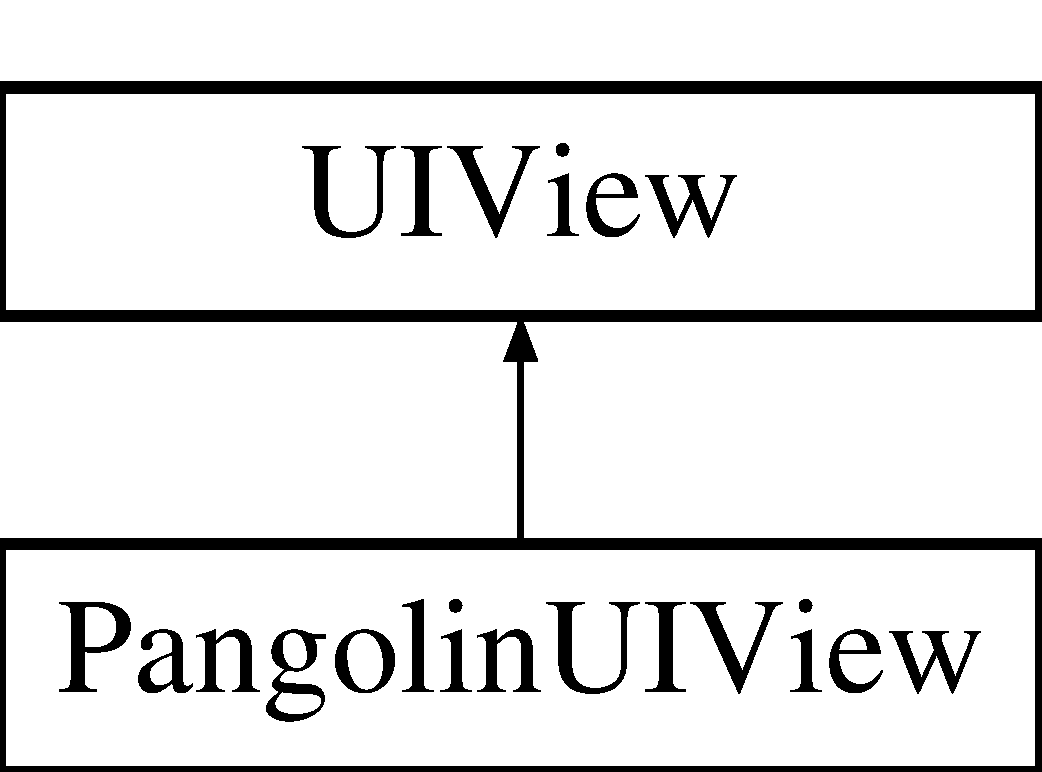
\includegraphics[height=2.000000cm]{interface_pangolin_u_i_view}
\end{center}
\end{figure}
\subsection*{Protected Attributes}
\begin{DoxyCompactItemize}
\item 
C\+A\+E\+A\+G\+L\+Layer $\ast$ {\bfseries \+\_\+eagl\+Layer}\hypertarget{interface_pangolin_u_i_view_a12215e1b55f9948f45165f2e8bbfdad6}{}\label{interface_pangolin_u_i_view_a12215e1b55f9948f45165f2e8bbfdad6}

\item 
E\+A\+G\+L\+Context $\ast$ {\bfseries \+\_\+context}\hypertarget{interface_pangolin_u_i_view_a0389238054102910b994cf7c8cb7a94c}{}\label{interface_pangolin_u_i_view_a0389238054102910b994cf7c8cb7a94c}

\item 
G\+Luint {\bfseries \+\_\+color\+Render\+Buffer}\hypertarget{interface_pangolin_u_i_view_a8a0557e11f73f2a6716940659721f9ab}{}\label{interface_pangolin_u_i_view_a8a0557e11f73f2a6716940659721f9ab}

\item 
G\+Luint {\bfseries \+\_\+depth\+Render\+Buffer}\hypertarget{interface_pangolin_u_i_view_a1bab310bc19f9cc312e80c17ef737d8c}{}\label{interface_pangolin_u_i_view_a1bab310bc19f9cc312e80c17ef737d8c}

\end{DoxyCompactItemize}


The documentation for this class was generated from the following file\+:\begin{DoxyCompactItemize}
\item 
/home/gapo/meng/deps/pangolin/include/pangolin/ios/Pangolin\+U\+I\+View.\+h\end{DoxyCompactItemize}

\hypertarget{classpangolin_1_1_pango_video}{}\section{pangolin\+:\+:Pango\+Video Class Reference}
\label{classpangolin_1_1_pango_video}\index{pangolin\+::\+Pango\+Video@{pangolin\+::\+Pango\+Video}}
Inheritance diagram for pangolin\+:\+:Pango\+Video\+:\begin{figure}[H]
\begin{center}
\leavevmode
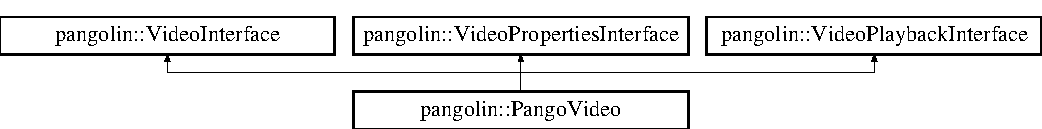
\includegraphics[height=1.736434cm]{classpangolin_1_1_pango_video}
\end{center}
\end{figure}
\subsection*{Public Member Functions}
\begin{DoxyCompactItemize}
\item 
{\bfseries Pango\+Video} (const std\+::string \&filename, bool realtime=true)\hypertarget{classpangolin_1_1_pango_video_a835d9bf15b58320383eed6fb2aa6e8d7}{}\label{classpangolin_1_1_pango_video_a835d9bf15b58320383eed6fb2aa6e8d7}

\item 
size\+\_\+t \hyperlink{classpangolin_1_1_pango_video_aed023430933996b5202799a3405cd388}{Size\+Bytes} () const P\+A\+N\+G\+O\+L\+I\+N\+\_\+\+O\+V\+E\+R\+R\+I\+DE\hypertarget{classpangolin_1_1_pango_video_aed023430933996b5202799a3405cd388}{}\label{classpangolin_1_1_pango_video_aed023430933996b5202799a3405cd388}

\begin{DoxyCompactList}\small\item\em Required buffer size to store all frames. \end{DoxyCompactList}\item 
const std\+::vector$<$ \hyperlink{classpangolin_1_1_stream_info}{Stream\+Info} $>$ \& \hyperlink{classpangolin_1_1_pango_video_a082c8deeda9600e96326eb6a312af11b}{Streams} () const P\+A\+N\+G\+O\+L\+I\+N\+\_\+\+O\+V\+E\+R\+R\+I\+DE\hypertarget{classpangolin_1_1_pango_video_a082c8deeda9600e96326eb6a312af11b}{}\label{classpangolin_1_1_pango_video_a082c8deeda9600e96326eb6a312af11b}

\begin{DoxyCompactList}\small\item\em Get format and dimensions of all video streams. \end{DoxyCompactList}\item 
void \hyperlink{classpangolin_1_1_pango_video_abc5f6c2942f1b7d946b67b411d82e682}{Start} () P\+A\+N\+G\+O\+L\+I\+N\+\_\+\+O\+V\+E\+R\+R\+I\+DE\hypertarget{classpangolin_1_1_pango_video_abc5f6c2942f1b7d946b67b411d82e682}{}\label{classpangolin_1_1_pango_video_abc5f6c2942f1b7d946b67b411d82e682}

\begin{DoxyCompactList}\small\item\em Start Video device. \end{DoxyCompactList}\item 
void \hyperlink{classpangolin_1_1_pango_video_a7978def8e5f13fff25225a045721f898}{Stop} () P\+A\+N\+G\+O\+L\+I\+N\+\_\+\+O\+V\+E\+R\+R\+I\+DE\hypertarget{classpangolin_1_1_pango_video_a7978def8e5f13fff25225a045721f898}{}\label{classpangolin_1_1_pango_video_a7978def8e5f13fff25225a045721f898}

\begin{DoxyCompactList}\small\item\em Stop Video device. \end{DoxyCompactList}\item 
bool \hyperlink{classpangolin_1_1_pango_video_abd49b114ac38554bbf29f4baa2d145ea}{Grab\+Next} (unsigned char $\ast$image, bool wait=true) P\+A\+N\+G\+O\+L\+I\+N\+\_\+\+O\+V\+E\+R\+R\+I\+DE
\begin{DoxyCompactList}\small\item\em Copy the next frame from the camera to image. \end{DoxyCompactList}\item 
bool \hyperlink{classpangolin_1_1_pango_video_a4968ca84a65d97cb87c5df1508d53655}{Grab\+Newest} (unsigned char $\ast$image, bool wait=true) P\+A\+N\+G\+O\+L\+I\+N\+\_\+\+O\+V\+E\+R\+R\+I\+DE
\begin{DoxyCompactList}\small\item\em Copy the newest frame from the camera to image discarding all older frames. \end{DoxyCompactList}\item 
const \hyperlink{classpangolin_1_1json_1_1value}{json\+::value} \& \hyperlink{classpangolin_1_1_pango_video_aeb10784316444180dacf7785dfa11784}{Device\+Properties} () const P\+A\+N\+G\+O\+L\+I\+N\+\_\+\+O\+V\+E\+R\+R\+I\+DE\hypertarget{classpangolin_1_1_pango_video_aeb10784316444180dacf7785dfa11784}{}\label{classpangolin_1_1_pango_video_aeb10784316444180dacf7785dfa11784}

\begin{DoxyCompactList}\small\item\em Access J\+S\+ON properties of device. \end{DoxyCompactList}\item 
const \hyperlink{classpangolin_1_1json_1_1value}{json\+::value} \& \hyperlink{classpangolin_1_1_pango_video_a1681ce549af0437857b0741c1161f420}{Frame\+Properties} () const P\+A\+N\+G\+O\+L\+I\+N\+\_\+\+O\+V\+E\+R\+R\+I\+DE\hypertarget{classpangolin_1_1_pango_video_a1681ce549af0437857b0741c1161f420}{}\label{classpangolin_1_1_pango_video_a1681ce549af0437857b0741c1161f420}

\begin{DoxyCompactList}\small\item\em Access J\+S\+ON properties of most recently captured frame. \end{DoxyCompactList}\item 
int \hyperlink{classpangolin_1_1_pango_video_a02cf8a9313c3826fdcf1e299ee8b9013}{Get\+Current\+Frame\+Id} () const P\+A\+N\+G\+O\+L\+I\+N\+\_\+\+O\+V\+E\+R\+R\+I\+DE\hypertarget{classpangolin_1_1_pango_video_a02cf8a9313c3826fdcf1e299ee8b9013}{}\label{classpangolin_1_1_pango_video_a02cf8a9313c3826fdcf1e299ee8b9013}

\begin{DoxyCompactList}\small\item\em Return monotonic id of current frame. \end{DoxyCompactList}\item 
int \hyperlink{classpangolin_1_1_pango_video_af6c22038f6e41b16f34ca08d7c82fec2}{Get\+Total\+Frames} () const P\+A\+N\+G\+O\+L\+I\+N\+\_\+\+O\+V\+E\+R\+R\+I\+DE
\begin{DoxyCompactList}\small\item\em Return total number of frames to be captured from device, or std\+::numeric\+\_\+limits$<$int$>$\+::max() on failure. \end{DoxyCompactList}\item 
int \hyperlink{classpangolin_1_1_pango_video_a7285cb5a18bcdf1e938dbcdbc9b54b37}{Seek} (int frameid) P\+A\+N\+G\+O\+L\+I\+N\+\_\+\+O\+V\+E\+R\+R\+I\+DE\hypertarget{classpangolin_1_1_pango_video_a7285cb5a18bcdf1e938dbcdbc9b54b37}{}\label{classpangolin_1_1_pango_video_a7285cb5a18bcdf1e938dbcdbc9b54b37}

\begin{DoxyCompactList}\small\item\em Return -\/1 on failure, frameid on success. \end{DoxyCompactList}\end{DoxyCompactItemize}
\subsection*{Protected Member Functions}
\begin{DoxyCompactItemize}
\item 
int {\bfseries Find\+Source} ()\hypertarget{classpangolin_1_1_pango_video_a9b00559cacf5e721d5b0bda29d39d05c}{}\label{classpangolin_1_1_pango_video_a9b00559cacf5e721d5b0bda29d39d05c}

\end{DoxyCompactItemize}
\subsection*{Protected Attributes}
\begin{DoxyCompactItemize}
\item 
\hyperlink{classpangolin_1_1_packet_stream_reader}{Packet\+Stream\+Reader} {\bfseries reader}\hypertarget{classpangolin_1_1_pango_video_a1d6589328e5dcbb0a6bcf21ed6b7477c}{}\label{classpangolin_1_1_pango_video_a1d6589328e5dcbb0a6bcf21ed6b7477c}

\item 
size\+\_\+t {\bfseries size\+\_\+bytes}\hypertarget{classpangolin_1_1_pango_video_afd22d0fbd6f350e7e5f40eafc3e97801}{}\label{classpangolin_1_1_pango_video_afd22d0fbd6f350e7e5f40eafc3e97801}

\item 
std\+::vector$<$ \hyperlink{classpangolin_1_1_stream_info}{Stream\+Info} $>$ {\bfseries streams}\hypertarget{classpangolin_1_1_pango_video_a09ae4a03fc3ba838fb462727ee892a5e}{}\label{classpangolin_1_1_pango_video_a09ae4a03fc3ba838fb462727ee892a5e}

\item 
\hyperlink{classpangolin_1_1json_1_1value}{json\+::value} {\bfseries device\+\_\+properties}\hypertarget{classpangolin_1_1_pango_video_a560fdeab226aa558afa2257e04a81001}{}\label{classpangolin_1_1_pango_video_a560fdeab226aa558afa2257e04a81001}

\item 
\hyperlink{classpangolin_1_1json_1_1value}{json\+::value} {\bfseries frame\+\_\+properties}\hypertarget{classpangolin_1_1_pango_video_a7d2778cfb6a216ae9c264f51cd2e0474}{}\label{classpangolin_1_1_pango_video_a7d2778cfb6a216ae9c264f51cd2e0474}

\item 
int {\bfseries src\+\_\+id}\hypertarget{classpangolin_1_1_pango_video_a273b4bda5c65d99cd41a95b590cbb56d}{}\label{classpangolin_1_1_pango_video_a273b4bda5c65d99cd41a95b590cbb56d}

\item 
int {\bfseries frame\+\_\+id}\hypertarget{classpangolin_1_1_pango_video_aae49ceda3a0d883f9a8d4fcb1d80172e}{}\label{classpangolin_1_1_pango_video_aae49ceda3a0d883f9a8d4fcb1d80172e}

\end{DoxyCompactItemize}


\subsection{Member Function Documentation}
\index{pangolin\+::\+Pango\+Video@{pangolin\+::\+Pango\+Video}!Get\+Total\+Frames@{Get\+Total\+Frames}}
\index{Get\+Total\+Frames@{Get\+Total\+Frames}!pangolin\+::\+Pango\+Video@{pangolin\+::\+Pango\+Video}}
\subsubsection[{\texorpdfstring{Get\+Total\+Frames() const P\+A\+N\+G\+O\+L\+I\+N\+\_\+\+O\+V\+E\+R\+R\+I\+DE}{GetTotalFrames() const PANGOLIN_OVERRIDE}}]{\setlength{\rightskip}{0pt plus 5cm}int pangolin\+::\+Pango\+Video\+::\+Get\+Total\+Frames (
\begin{DoxyParamCaption}
{}
\end{DoxyParamCaption}
) const\hspace{0.3cm}{\ttfamily [virtual]}}\hypertarget{classpangolin_1_1_pango_video_af6c22038f6e41b16f34ca08d7c82fec2}{}\label{classpangolin_1_1_pango_video_af6c22038f6e41b16f34ca08d7c82fec2}


Return total number of frames to be captured from device, or std\+::numeric\+\_\+limits$<$int$>$\+::max() on failure. 



Implements \hyperlink{structpangolin_1_1_video_playback_interface_aa1ab605b49009c52a80eaa0cc074b63b}{pangolin\+::\+Video\+Playback\+Interface}.

\index{pangolin\+::\+Pango\+Video@{pangolin\+::\+Pango\+Video}!Grab\+Newest@{Grab\+Newest}}
\index{Grab\+Newest@{Grab\+Newest}!pangolin\+::\+Pango\+Video@{pangolin\+::\+Pango\+Video}}
\subsubsection[{\texorpdfstring{Grab\+Newest(unsigned char $\ast$image, bool wait=true) P\+A\+N\+G\+O\+L\+I\+N\+\_\+\+O\+V\+E\+R\+R\+I\+DE}{GrabNewest(unsigned char *image, bool wait=true) PANGOLIN_OVERRIDE}}]{\setlength{\rightskip}{0pt plus 5cm}bool pangolin\+::\+Pango\+Video\+::\+Grab\+Newest (
\begin{DoxyParamCaption}
\item[{unsigned char $\ast$}]{image, }
\item[{bool}]{wait = {\ttfamily true}}
\end{DoxyParamCaption}
)\hspace{0.3cm}{\ttfamily [virtual]}}\hypertarget{classpangolin_1_1_pango_video_a4968ca84a65d97cb87c5df1508d53655}{}\label{classpangolin_1_1_pango_video_a4968ca84a65d97cb87c5df1508d53655}


Copy the newest frame from the camera to image discarding all older frames. 

Optionally wait for a frame if one isn\textquotesingle{}t ready Returns true iff image was copied 

Implements \hyperlink{structpangolin_1_1_video_interface_a062ad8f58e023e93ce48b1c61ea00674}{pangolin\+::\+Video\+Interface}.

\index{pangolin\+::\+Pango\+Video@{pangolin\+::\+Pango\+Video}!Grab\+Next@{Grab\+Next}}
\index{Grab\+Next@{Grab\+Next}!pangolin\+::\+Pango\+Video@{pangolin\+::\+Pango\+Video}}
\subsubsection[{\texorpdfstring{Grab\+Next(unsigned char $\ast$image, bool wait=true) P\+A\+N\+G\+O\+L\+I\+N\+\_\+\+O\+V\+E\+R\+R\+I\+DE}{GrabNext(unsigned char *image, bool wait=true) PANGOLIN_OVERRIDE}}]{\setlength{\rightskip}{0pt plus 5cm}bool pangolin\+::\+Pango\+Video\+::\+Grab\+Next (
\begin{DoxyParamCaption}
\item[{unsigned char $\ast$}]{image, }
\item[{bool}]{wait = {\ttfamily true}}
\end{DoxyParamCaption}
)\hspace{0.3cm}{\ttfamily [virtual]}}\hypertarget{classpangolin_1_1_pango_video_abd49b114ac38554bbf29f4baa2d145ea}{}\label{classpangolin_1_1_pango_video_abd49b114ac38554bbf29f4baa2d145ea}


Copy the next frame from the camera to image. 

Optionally wait for a frame if one isn\textquotesingle{}t ready Returns true iff image was copied 

Implements \hyperlink{structpangolin_1_1_video_interface_a2a87c2219959a762dbbb43760d27ff27}{pangolin\+::\+Video\+Interface}.



The documentation for this class was generated from the following file\+:\begin{DoxyCompactItemize}
\item 
/home/gapo/meng/deps/pangolin/include/pangolin/video/drivers/pango\+\_\+video.\+h\end{DoxyCompactItemize}

\hypertarget{classpangolin_1_1_pango_video_output}{}\section{pangolin\+:\+:Pango\+Video\+Output Class Reference}
\label{classpangolin_1_1_pango_video_output}\index{pangolin\+::\+Pango\+Video\+Output@{pangolin\+::\+Pango\+Video\+Output}}
Inheritance diagram for pangolin\+:\+:Pango\+Video\+Output\+:\begin{figure}[H]
\begin{center}
\leavevmode
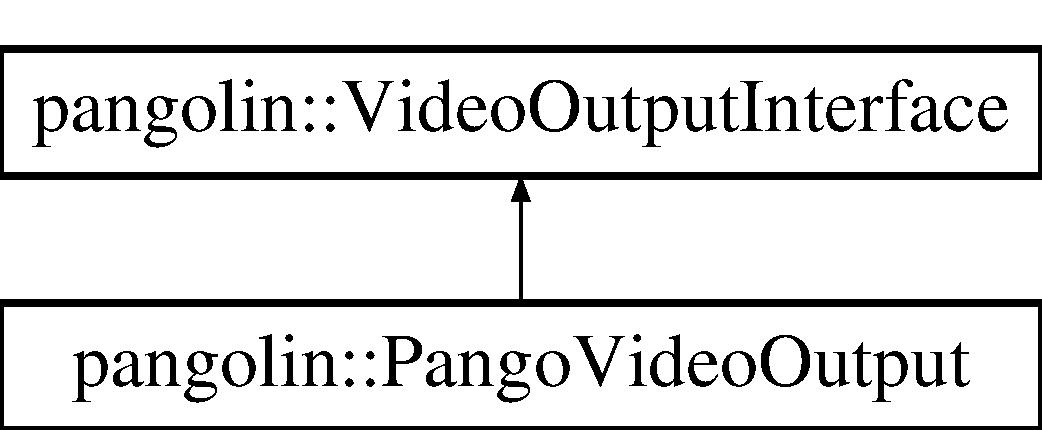
\includegraphics[height=2.000000cm]{classpangolin_1_1_pango_video_output}
\end{center}
\end{figure}
\subsection*{Public Member Functions}
\begin{DoxyCompactItemize}
\item 
{\bfseries Pango\+Video\+Output} (const std\+::string \&filename)\hypertarget{classpangolin_1_1_pango_video_output_aec31206b29c247ca1f7d398000a10392}{}\label{classpangolin_1_1_pango_video_output_aec31206b29c247ca1f7d398000a10392}

\item 
const std\+::vector$<$ \hyperlink{classpangolin_1_1_stream_info}{Stream\+Info} $>$ \& \hyperlink{classpangolin_1_1_pango_video_output_ac23bcb781e1bea1a76643ab2e425826e}{Streams} () const P\+A\+N\+G\+O\+L\+I\+N\+\_\+\+O\+V\+E\+R\+R\+I\+DE\hypertarget{classpangolin_1_1_pango_video_output_ac23bcb781e1bea1a76643ab2e425826e}{}\label{classpangolin_1_1_pango_video_output_ac23bcb781e1bea1a76643ab2e425826e}

\begin{DoxyCompactList}\small\item\em Get format and dimensions of all video streams. \end{DoxyCompactList}\item 
void {\bfseries Set\+Streams} (const std\+::vector$<$ \hyperlink{classpangolin_1_1_stream_info}{Stream\+Info} $>$ \&streams, const std\+::string \&uri, const \hyperlink{classpangolin_1_1json_1_1value}{json\+::value} \&device\+\_\+properties) P\+A\+N\+G\+O\+L\+I\+N\+\_\+\+O\+V\+E\+R\+R\+I\+DE\hypertarget{classpangolin_1_1_pango_video_output_a0538af17827c5a94d32c35206cb066ed}{}\label{classpangolin_1_1_pango_video_output_a0538af17827c5a94d32c35206cb066ed}

\item 
int {\bfseries Write\+Streams} (unsigned char $\ast$data, const \hyperlink{classpangolin_1_1json_1_1value}{json\+::value} \&frame\+\_\+properties) P\+A\+N\+G\+O\+L\+I\+N\+\_\+\+O\+V\+E\+R\+R\+I\+DE\hypertarget{classpangolin_1_1_pango_video_output_afe472eb97d705bbcbbade0bcf3f0371e}{}\label{classpangolin_1_1_pango_video_output_afe472eb97d705bbcbbade0bcf3f0371e}

\end{DoxyCompactItemize}
\subsection*{Protected Member Functions}
\begin{DoxyCompactItemize}
\item 
void {\bfseries Write\+Header} ()\hypertarget{classpangolin_1_1_pango_video_output_acf9b87c98d03f3305a20deaf43f7d9c5}{}\label{classpangolin_1_1_pango_video_output_acf9b87c98d03f3305a20deaf43f7d9c5}

\end{DoxyCompactItemize}
\subsection*{Protected Attributes}
\begin{DoxyCompactItemize}
\item 
std\+::vector$<$ \hyperlink{classpangolin_1_1_stream_info}{Stream\+Info} $>$ {\bfseries streams}\hypertarget{classpangolin_1_1_pango_video_output_ae873edc5549ace0762cc521040984dc2}{}\label{classpangolin_1_1_pango_video_output_ae873edc5549ace0762cc521040984dc2}

\item 
std\+::string {\bfseries input\+\_\+uri}\hypertarget{classpangolin_1_1_pango_video_output_adb0087393170be08d938f64f182e8cc9}{}\label{classpangolin_1_1_pango_video_output_adb0087393170be08d938f64f182e8cc9}

\item 
\hyperlink{classpangolin_1_1json_1_1value}{json\+::value} {\bfseries device\+\_\+properties}\hypertarget{classpangolin_1_1_pango_video_output_a04736e7c26993f17fdc02e2ff1f44eeb}{}\label{classpangolin_1_1_pango_video_output_a04736e7c26993f17fdc02e2ff1f44eeb}

\item 
\hyperlink{classpangolin_1_1_packet_stream_writer}{Packet\+Stream\+Writer} {\bfseries packetstream}\hypertarget{classpangolin_1_1_pango_video_output_ac0a01e6bb235387ade3c258e36f43b84}{}\label{classpangolin_1_1_pango_video_output_ac0a01e6bb235387ade3c258e36f43b84}

\item 
int {\bfseries packetstreamsrcid}\hypertarget{classpangolin_1_1_pango_video_output_abb9eecefc2aed72a623760a48765374c}{}\label{classpangolin_1_1_pango_video_output_abb9eecefc2aed72a623760a48765374c}

\item 
size\+\_\+t {\bfseries total\+\_\+frame\+\_\+size}\hypertarget{classpangolin_1_1_pango_video_output_abb26b19fd1e68fd35f5f85f68337aade}{}\label{classpangolin_1_1_pango_video_output_abb26b19fd1e68fd35f5f85f68337aade}

\end{DoxyCompactItemize}


The documentation for this class was generated from the following file\+:\begin{DoxyCompactItemize}
\item 
/home/gapo/meng/deps/pangolin/include/pangolin/video/drivers/pango\+\_\+video\+\_\+output.\+h\end{DoxyCompactItemize}

\hypertarget{classpangolin_1_1_params}{}\section{pangolin\+:\+:Params Class Reference}
\label{classpangolin_1_1_params}\index{pangolin\+::\+Params@{pangolin\+::\+Params}}
Inheritance diagram for pangolin\+:\+:Params\+:\begin{figure}[H]
\begin{center}
\leavevmode
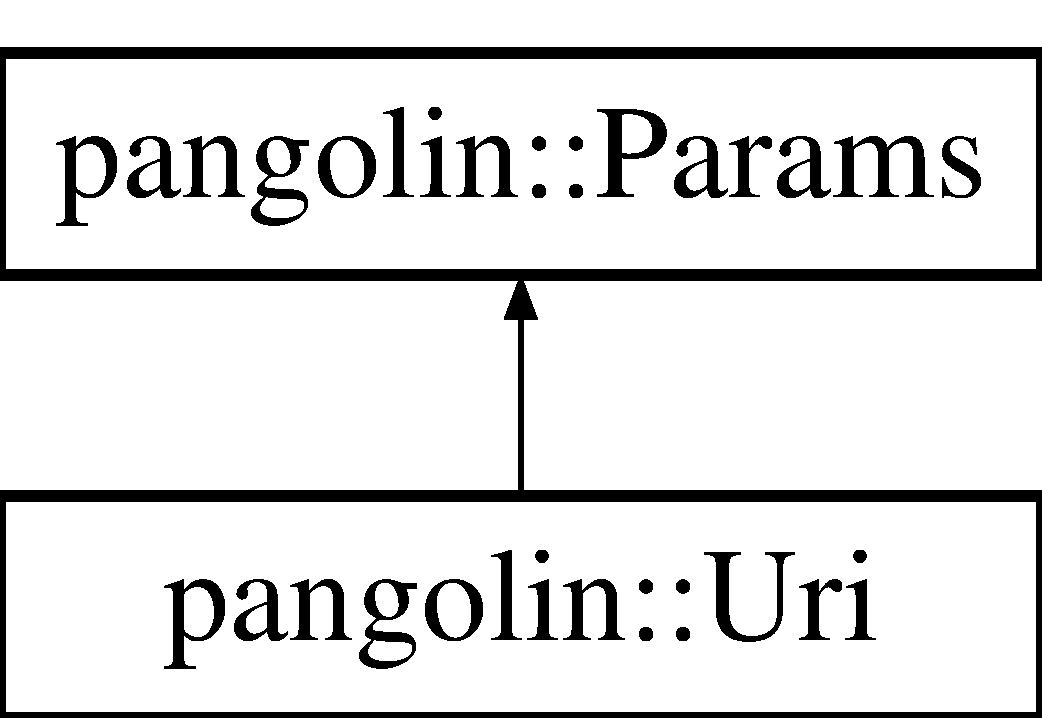
\includegraphics[height=2.000000cm]{classpangolin_1_1_params}
\end{center}
\end{figure}
\subsection*{Public Types}
\begin{DoxyCompactItemize}
\item 
typedef std\+::map$<$ std\+::string, std\+::string $>$ {\bfseries Param\+Map}\hypertarget{classpangolin_1_1_params_a4f1caed253e04e835e5e3ece9d29ba48}{}\label{classpangolin_1_1_params_a4f1caed253e04e835e5e3ece9d29ba48}

\end{DoxyCompactItemize}
\subsection*{Public Member Functions}
\begin{DoxyCompactItemize}
\item 
bool {\bfseries Contains} (const std\+::string \&key) const \hypertarget{classpangolin_1_1_params_acebceaa4f09c02b7efb79147ff26c001}{}\label{classpangolin_1_1_params_acebceaa4f09c02b7efb79147ff26c001}

\item 
{\footnotesize template$<$typename T $>$ }\\T {\bfseries Get} (const std\+::string \&key, T default\+\_\+val) const \hypertarget{classpangolin_1_1_params_ad0aa5e8b0130a58a94a44dfd8b1cb7ca}{}\label{classpangolin_1_1_params_ad0aa5e8b0130a58a94a44dfd8b1cb7ca}

\item 
{\footnotesize template$<$typename T $>$ }\\void {\bfseries Set} (const std\+::string \&key, const T \&val)\hypertarget{classpangolin_1_1_params_a9278b5ab08ff14f3318c21fd35d2a967}{}\label{classpangolin_1_1_params_a9278b5ab08ff14f3318c21fd35d2a967}

\end{DoxyCompactItemize}
\subsection*{Public Attributes}
\begin{DoxyCompactItemize}
\item 
Param\+Map {\bfseries params}\hypertarget{classpangolin_1_1_params_a03130e8d576709a8dd06a7776e09a26e}{}\label{classpangolin_1_1_params_a03130e8d576709a8dd06a7776e09a26e}

\end{DoxyCompactItemize}


The documentation for this class was generated from the following file\+:\begin{DoxyCompactItemize}
\item 
/home/gapo/meng/deps/pangolin/include/pangolin/utils/params.\+h\end{DoxyCompactItemize}

\hypertarget{classpangolin_1_1_pleora_video}{}\section{pangolin\+:\+:Pleora\+Video Class Reference}
\label{classpangolin_1_1_pleora_video}\index{pangolin\+::\+Pleora\+Video@{pangolin\+::\+Pleora\+Video}}
Inheritance diagram for pangolin\+:\+:Pleora\+Video\+:\begin{figure}[H]
\begin{center}
\leavevmode
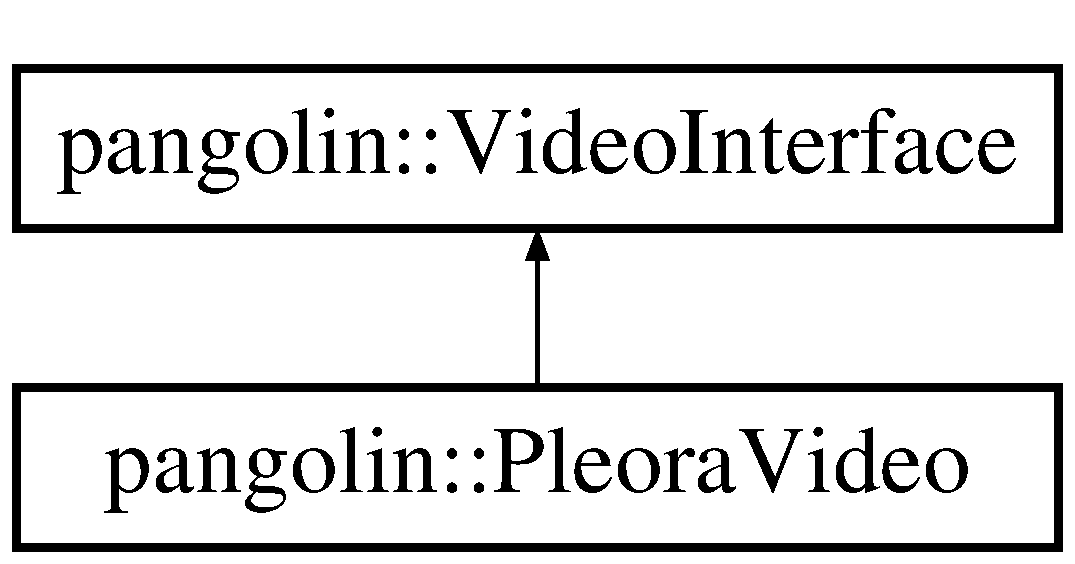
\includegraphics[height=2.000000cm]{classpangolin_1_1_pleora_video}
\end{center}
\end{figure}
\subsection*{Public Member Functions}
\begin{DoxyCompactItemize}
\item 
{\bfseries Pleora\+Video} (const char $\ast$model\+\_\+name, const char $\ast$serial\+\_\+num, size\+\_\+t index, size\+\_\+t bpp=8, size\+\_\+t binX=1, size\+\_\+t binY=1, size\+\_\+t buffer\+\_\+count=4, size\+\_\+t desired\+\_\+size\+\_\+x=0, size\+\_\+t desired\+\_\+size\+\_\+y=0, size\+\_\+t desired\+\_\+pos\+\_\+x=0, size\+\_\+t desired\+\_\+pos\+\_\+y=0)\hypertarget{classpangolin_1_1_pleora_video_af5de7d30e0b8287d2c63386610ead49b}{}\label{classpangolin_1_1_pleora_video_af5de7d30e0b8287d2c63386610ead49b}

\item 
void \hyperlink{classpangolin_1_1_pleora_video_a577b97426c315ddeb29446fcd1c8acda}{Start} ()\hypertarget{classpangolin_1_1_pleora_video_a577b97426c315ddeb29446fcd1c8acda}{}\label{classpangolin_1_1_pleora_video_a577b97426c315ddeb29446fcd1c8acda}

\begin{DoxyCompactList}\small\item\em Start Video device. \end{DoxyCompactList}\item 
void \hyperlink{classpangolin_1_1_pleora_video_aed12ed85d97d258096a8e6ce19c048e2}{Stop} ()\hypertarget{classpangolin_1_1_pleora_video_aed12ed85d97d258096a8e6ce19c048e2}{}\label{classpangolin_1_1_pleora_video_aed12ed85d97d258096a8e6ce19c048e2}

\begin{DoxyCompactList}\small\item\em Stop Video device. \end{DoxyCompactList}\item 
size\+\_\+t \hyperlink{classpangolin_1_1_pleora_video_af608d7d12abeb6a941f4f1d2de914e8e}{Size\+Bytes} () const \hypertarget{classpangolin_1_1_pleora_video_af608d7d12abeb6a941f4f1d2de914e8e}{}\label{classpangolin_1_1_pleora_video_af608d7d12abeb6a941f4f1d2de914e8e}

\begin{DoxyCompactList}\small\item\em Required buffer size to store all frames. \end{DoxyCompactList}\item 
const std\+::vector$<$ \hyperlink{classpangolin_1_1_stream_info}{Stream\+Info} $>$ \& \hyperlink{classpangolin_1_1_pleora_video_a25e41a13969a979657343971d97043aa}{Streams} () const \hypertarget{classpangolin_1_1_pleora_video_a25e41a13969a979657343971d97043aa}{}\label{classpangolin_1_1_pleora_video_a25e41a13969a979657343971d97043aa}

\begin{DoxyCompactList}\small\item\em Get format and dimensions of all video streams. \end{DoxyCompactList}\item 
bool \hyperlink{classpangolin_1_1_pleora_video_aa9c01e6f43cebefb05aaaf847292de04}{Grab\+Next} (unsigned char $\ast$image, bool wait=true)
\begin{DoxyCompactList}\small\item\em Copy the next frame from the camera to image. \end{DoxyCompactList}\item 
bool \hyperlink{classpangolin_1_1_pleora_video_ae1984dd3f892a8cad426e692e21c6fb4}{Grab\+Newest} (unsigned char $\ast$image, bool wait=true)
\begin{DoxyCompactList}\small\item\em Copy the newest frame from the camera to image discarding all older frames. \end{DoxyCompactList}\end{DoxyCompactItemize}
\subsection*{Protected Member Functions}
\begin{DoxyCompactItemize}
\item 
{\footnotesize template$<$typename T $>$ }\\T {\bfseries Device\+Param} (const char $\ast$name)\hypertarget{classpangolin_1_1_pleora_video_a1d8195f4e6e01ef524320be368acb1b0}{}\label{classpangolin_1_1_pleora_video_a1d8195f4e6e01ef524320be368acb1b0}

\item 
{\footnotesize template$<$typename T $>$ }\\T {\bfseries Stream\+Param} (const char $\ast$name)\hypertarget{classpangolin_1_1_pleora_video_ad1b5da5a21c2fd9c56240a4962293131}{}\label{classpangolin_1_1_pleora_video_ad1b5da5a21c2fd9c56240a4962293131}

\end{DoxyCompactItemize}
\subsection*{Protected Attributes}
\begin{DoxyCompactItemize}
\item 
std\+::vector$<$ \hyperlink{classpangolin_1_1_stream_info}{Stream\+Info} $>$ {\bfseries streams}\hypertarget{classpangolin_1_1_pleora_video_a8171b50fed4fcc81cb3881d09d1510b3}{}\label{classpangolin_1_1_pleora_video_a8171b50fed4fcc81cb3881d09d1510b3}

\item 
size\+\_\+t {\bfseries size\+\_\+bytes}\hypertarget{classpangolin_1_1_pleora_video_a49b0a13b0f51b2cd55ba5896f674691f}{}\label{classpangolin_1_1_pleora_video_a49b0a13b0f51b2cd55ba5896f674691f}

\item 
Pv\+System $\ast$ {\bfseries l\+Pv\+System}\hypertarget{classpangolin_1_1_pleora_video_a1d07f01e5d2baaec4975726054f0374e}{}\label{classpangolin_1_1_pleora_video_a1d07f01e5d2baaec4975726054f0374e}

\item 
Pv\+Device $\ast$ {\bfseries l\+Device}\hypertarget{classpangolin_1_1_pleora_video_acf9169162a19fcaa2747fa71b8c2daad}{}\label{classpangolin_1_1_pleora_video_acf9169162a19fcaa2747fa71b8c2daad}

\item 
Pv\+Stream $\ast$ {\bfseries l\+Stream}\hypertarget{classpangolin_1_1_pleora_video_a329db77619472aa110c16d1d1b4d9167}{}\label{classpangolin_1_1_pleora_video_a329db77619472aa110c16d1d1b4d9167}

\item 
Pv\+Gen\+Parameter\+Array $\ast$ {\bfseries l\+Device\+Params}\hypertarget{classpangolin_1_1_pleora_video_a350c0a8c52cc75e49c2edacaf7428121}{}\label{classpangolin_1_1_pleora_video_a350c0a8c52cc75e49c2edacaf7428121}

\item 
Pv\+Gen\+Command $\ast$ {\bfseries l\+Start}\hypertarget{classpangolin_1_1_pleora_video_a7c6977d724218b751f2b3c9a703995c5}{}\label{classpangolin_1_1_pleora_video_a7c6977d724218b751f2b3c9a703995c5}

\item 
Pv\+Gen\+Command $\ast$ {\bfseries l\+Stop}\hypertarget{classpangolin_1_1_pleora_video_a4d6a07614ae15e921dec962137666956}{}\label{classpangolin_1_1_pleora_video_a4d6a07614ae15e921dec962137666956}

\item 
Pv\+Gen\+Parameter\+Array $\ast$ {\bfseries l\+Stream\+Params}\hypertarget{classpangolin_1_1_pleora_video_a2ee2cb5a246856ec29b5fca7b7276b51}{}\label{classpangolin_1_1_pleora_video_a2ee2cb5a246856ec29b5fca7b7276b51}

\item 
Buffer\+List {\bfseries l\+Buffer\+List}\hypertarget{classpangolin_1_1_pleora_video_a833ff4a806cb846af4c5a3ee6f7db761}{}\label{classpangolin_1_1_pleora_video_a833ff4a806cb846af4c5a3ee6f7db761}

\end{DoxyCompactItemize}


\subsection{Member Function Documentation}
\index{pangolin\+::\+Pleora\+Video@{pangolin\+::\+Pleora\+Video}!Grab\+Newest@{Grab\+Newest}}
\index{Grab\+Newest@{Grab\+Newest}!pangolin\+::\+Pleora\+Video@{pangolin\+::\+Pleora\+Video}}
\subsubsection[{\texorpdfstring{Grab\+Newest(unsigned char $\ast$image, bool wait=true)}{GrabNewest(unsigned char *image, bool wait=true)}}]{\setlength{\rightskip}{0pt plus 5cm}bool pangolin\+::\+Pleora\+Video\+::\+Grab\+Newest (
\begin{DoxyParamCaption}
\item[{unsigned char $\ast$}]{image, }
\item[{bool}]{wait = {\ttfamily true}}
\end{DoxyParamCaption}
)\hspace{0.3cm}{\ttfamily [virtual]}}\hypertarget{classpangolin_1_1_pleora_video_ae1984dd3f892a8cad426e692e21c6fb4}{}\label{classpangolin_1_1_pleora_video_ae1984dd3f892a8cad426e692e21c6fb4}


Copy the newest frame from the camera to image discarding all older frames. 

Optionally wait for a frame if one isn\textquotesingle{}t ready Returns true iff image was copied 

Implements \hyperlink{structpangolin_1_1_video_interface_a062ad8f58e023e93ce48b1c61ea00674}{pangolin\+::\+Video\+Interface}.

\index{pangolin\+::\+Pleora\+Video@{pangolin\+::\+Pleora\+Video}!Grab\+Next@{Grab\+Next}}
\index{Grab\+Next@{Grab\+Next}!pangolin\+::\+Pleora\+Video@{pangolin\+::\+Pleora\+Video}}
\subsubsection[{\texorpdfstring{Grab\+Next(unsigned char $\ast$image, bool wait=true)}{GrabNext(unsigned char *image, bool wait=true)}}]{\setlength{\rightskip}{0pt plus 5cm}bool pangolin\+::\+Pleora\+Video\+::\+Grab\+Next (
\begin{DoxyParamCaption}
\item[{unsigned char $\ast$}]{image, }
\item[{bool}]{wait = {\ttfamily true}}
\end{DoxyParamCaption}
)\hspace{0.3cm}{\ttfamily [virtual]}}\hypertarget{classpangolin_1_1_pleora_video_aa9c01e6f43cebefb05aaaf847292de04}{}\label{classpangolin_1_1_pleora_video_aa9c01e6f43cebefb05aaaf847292de04}


Copy the next frame from the camera to image. 

Optionally wait for a frame if one isn\textquotesingle{}t ready Returns true iff image was copied 

Implements \hyperlink{structpangolin_1_1_video_interface_a2a87c2219959a762dbbb43760d27ff27}{pangolin\+::\+Video\+Interface}.



The documentation for this class was generated from the following file\+:\begin{DoxyCompactItemize}
\item 
/home/gapo/meng/deps/pangolin/include/pangolin/video/drivers/pleora.\+h\end{DoxyCompactItemize}

\hypertarget{structpangolin_1_1_plotter_1_1_plot_attrib}{}\section{pangolin\+:\+:Plotter\+:\+:Plot\+Attrib Struct Reference}
\label{structpangolin_1_1_plotter_1_1_plot_attrib}\index{pangolin\+::\+Plotter\+::\+Plot\+Attrib@{pangolin\+::\+Plotter\+::\+Plot\+Attrib}}
\subsection*{Public Member Functions}
\begin{DoxyCompactItemize}
\item 
{\bfseries Plot\+Attrib} (std\+::string name, int plot\+\_\+id, int location=-\/1)\hypertarget{structpangolin_1_1_plotter_1_1_plot_attrib_ae0a3f847da9c09f33e0806214bf09bda}{}\label{structpangolin_1_1_plotter_1_1_plot_attrib_ae0a3f847da9c09f33e0806214bf09bda}

\end{DoxyCompactItemize}
\subsection*{Public Attributes}
\begin{DoxyCompactItemize}
\item 
std\+::string {\bfseries name}\hypertarget{structpangolin_1_1_plotter_1_1_plot_attrib_a1e6f02a847fb68c99aa801517198f934}{}\label{structpangolin_1_1_plotter_1_1_plot_attrib_a1e6f02a847fb68c99aa801517198f934}

\item 
int {\bfseries plot\+\_\+id}\hypertarget{structpangolin_1_1_plotter_1_1_plot_attrib_af7844bf50d80ed36b5320b78900272ca}{}\label{structpangolin_1_1_plotter_1_1_plot_attrib_af7844bf50d80ed36b5320b78900272ca}

\item 
int {\bfseries location}\hypertarget{structpangolin_1_1_plotter_1_1_plot_attrib_ab796fecc0847b017250f67e8f5e5eb73}{}\label{structpangolin_1_1_plotter_1_1_plot_attrib_ab796fecc0847b017250f67e8f5e5eb73}

\end{DoxyCompactItemize}


The documentation for this struct was generated from the following file\+:\begin{DoxyCompactItemize}
\item 
/home/gapo/meng/deps/pangolin/include/pangolin/plot/plotter.\+h\end{DoxyCompactItemize}

\hypertarget{structpangolin_1_1_plotter_1_1_plot_implicit}{}\section{pangolin\+:\+:Plotter\+:\+:Plot\+Implicit Struct Reference}
\label{structpangolin_1_1_plotter_1_1_plot_implicit}\index{pangolin\+::\+Plotter\+::\+Plot\+Implicit@{pangolin\+::\+Plotter\+::\+Plot\+Implicit}}
\subsection*{Public Member Functions}
\begin{DoxyCompactItemize}
\item 
void {\bfseries Create\+Plot} (const std\+::string \&code)\hypertarget{structpangolin_1_1_plotter_1_1_plot_implicit_a8fe873d5c02f53918e6701fe42143c2a}{}\label{structpangolin_1_1_plotter_1_1_plot_implicit_a8fe873d5c02f53918e6701fe42143c2a}

\item 
void {\bfseries Create\+Coloured\+Plot} (const std\+::string \&code)\hypertarget{structpangolin_1_1_plotter_1_1_plot_implicit_a8cd8860e9b38a349da94e281b7d48ad9}{}\label{structpangolin_1_1_plotter_1_1_plot_implicit_a8cd8860e9b38a349da94e281b7d48ad9}

\item 
void {\bfseries Create\+Inequality} (const std\+::string \&ie, \hyperlink{structpangolin_1_1_colour}{Colour} c)\hypertarget{structpangolin_1_1_plotter_1_1_plot_implicit_ad667885ee92a5458874f01784b61796c}{}\label{structpangolin_1_1_plotter_1_1_plot_implicit_ad667885ee92a5458874f01784b61796c}

\item 
void {\bfseries Create\+Distance\+Plot} (const std\+::string \&dist)\hypertarget{structpangolin_1_1_plotter_1_1_plot_implicit_a5d206dc4f3c2ac5fffeecdc505e22d13}{}\label{structpangolin_1_1_plotter_1_1_plot_implicit_a5d206dc4f3c2ac5fffeecdc505e22d13}

\end{DoxyCompactItemize}
\subsection*{Public Attributes}
\begin{DoxyCompactItemize}
\item 
\hyperlink{classpangolin_1_1_gl_sl_program}{Gl\+Sl\+Program} {\bfseries prog}\hypertarget{structpangolin_1_1_plotter_1_1_plot_implicit_a4880a9c7a401c34ba55beb8d76916548}{}\label{structpangolin_1_1_plotter_1_1_plot_implicit_a4880a9c7a401c34ba55beb8d76916548}

\end{DoxyCompactItemize}


The documentation for this struct was generated from the following file\+:\begin{DoxyCompactItemize}
\item 
/home/gapo/meng/deps/pangolin/include/pangolin/plot/plotter.\+h\end{DoxyCompactItemize}

\hypertarget{structpangolin_1_1_plotter_1_1_plot_series}{}\section{pangolin\+:\+:Plotter\+:\+:Plot\+Series Struct Reference}
\label{structpangolin_1_1_plotter_1_1_plot_series}\index{pangolin\+::\+Plotter\+::\+Plot\+Series@{pangolin\+::\+Plotter\+::\+Plot\+Series}}
\subsection*{Public Member Functions}
\begin{DoxyCompactItemize}
\item 
void {\bfseries Create\+Plot} (const std\+::string \&x, const std\+::string \&y, \hyperlink{structpangolin_1_1_colour}{Colour} c, std\+::string title)\hypertarget{structpangolin_1_1_plotter_1_1_plot_series_a772fbedf1f76b1bb26987a0e51bfa914}{}\label{structpangolin_1_1_plotter_1_1_plot_series_a772fbedf1f76b1bb26987a0e51bfa914}

\end{DoxyCompactItemize}
\subsection*{Public Attributes}
\begin{DoxyCompactItemize}
\item 
\hyperlink{classpangolin_1_1_gl_sl_program}{Gl\+Sl\+Program} {\bfseries prog}\hypertarget{structpangolin_1_1_plotter_1_1_plot_series_a0443889134161b24069807529ea0609b}{}\label{structpangolin_1_1_plotter_1_1_plot_series_a0443889134161b24069807529ea0609b}

\item 
\hyperlink{classpangolin_1_1_gl_text}{Gl\+Text} {\bfseries title}\hypertarget{structpangolin_1_1_plotter_1_1_plot_series_ac2bdf52f47e31491d983c4f06d098243}{}\label{structpangolin_1_1_plotter_1_1_plot_series_ac2bdf52f47e31491d983c4f06d098243}

\item 
bool {\bfseries contains\+\_\+id}\hypertarget{structpangolin_1_1_plotter_1_1_plot_series_a1d5eda377aa9316c2ed56f48c9a90782}{}\label{structpangolin_1_1_plotter_1_1_plot_series_a1d5eda377aa9316c2ed56f48c9a90782}

\item 
std\+::vector$<$ \hyperlink{structpangolin_1_1_plotter_1_1_plot_attrib}{Plot\+Attrib} $>$ {\bfseries attribs}\hypertarget{structpangolin_1_1_plotter_1_1_plot_series_aea39271d794d57a0c3485531d4d0a1a4}{}\label{structpangolin_1_1_plotter_1_1_plot_series_aea39271d794d57a0c3485531d4d0a1a4}

\item 
G\+Lenum {\bfseries drawing\+\_\+mode}\hypertarget{structpangolin_1_1_plotter_1_1_plot_series_aebef14bc3a2d65ce9862392f163e579b}{}\label{structpangolin_1_1_plotter_1_1_plot_series_aebef14bc3a2d65ce9862392f163e579b}

\item 
\hyperlink{structpangolin_1_1_colour}{Colour} {\bfseries colour}\hypertarget{structpangolin_1_1_plotter_1_1_plot_series_acc34aa72785115f44d771d6d3d5a4c2c}{}\label{structpangolin_1_1_plotter_1_1_plot_series_acc34aa72785115f44d771d6d3d5a4c2c}

\item 
bool {\bfseries used}\hypertarget{structpangolin_1_1_plotter_1_1_plot_series_af89701d1d669f9a5afe70c3c3a3c1eba}{}\label{structpangolin_1_1_plotter_1_1_plot_series_af89701d1d669f9a5afe70c3c3a3c1eba}

\end{DoxyCompactItemize}


The documentation for this struct was generated from the following file\+:\begin{DoxyCompactItemize}
\item 
/home/gapo/meng/deps/pangolin/include/pangolin/plot/plotter.\+h\end{DoxyCompactItemize}

\hypertarget{classpangolin_1_1_plotter}{}\section{pangolin\+:\+:Plotter Class Reference}
\label{classpangolin_1_1_plotter}\index{pangolin\+::\+Plotter@{pangolin\+::\+Plotter}}
Inheritance diagram for pangolin\+:\+:Plotter\+:\begin{figure}[H]
\begin{center}
\leavevmode
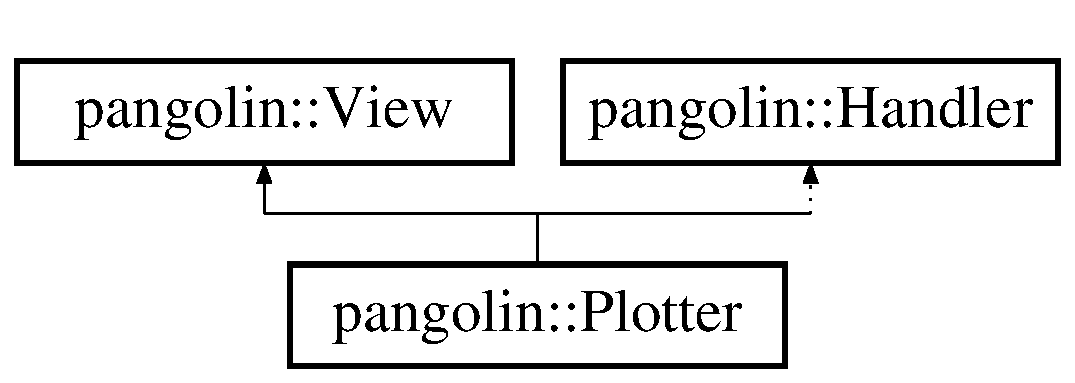
\includegraphics[height=2.000000cm]{classpangolin_1_1_plotter}
\end{center}
\end{figure}
\subsection*{Classes}
\begin{DoxyCompactItemize}
\item 
struct \hyperlink{structpangolin_1_1_plotter_1_1_plot_attrib}{Plot\+Attrib}
\item 
struct \hyperlink{structpangolin_1_1_plotter_1_1_plot_implicit}{Plot\+Implicit}
\item 
struct \hyperlink{structpangolin_1_1_plotter_1_1_plot_series}{Plot\+Series}
\item 
struct \hyperlink{structpangolin_1_1_plotter_1_1_tick}{Tick}
\end{DoxyCompactItemize}
\subsection*{Public Member Functions}
\begin{DoxyCompactItemize}
\item 
{\bfseries Plotter} (\hyperlink{classpangolin_1_1_data_log}{Data\+Log} $\ast$log, float left=0, float right=600, float bottom=-\/1, float top=1, float tickx=30, float ticky=0.\+5, \hyperlink{classpangolin_1_1_plotter}{Plotter} $\ast$linked\+\_\+plotter\+\_\+x=0, \hyperlink{classpangolin_1_1_plotter}{Plotter} $\ast$linked\+\_\+plotter\+\_\+y=0)\hypertarget{classpangolin_1_1_plotter_ad2fe719a5005597dabb043956775c683}{}\label{classpangolin_1_1_plotter_ad2fe719a5005597dabb043956775c683}

\item 
void \hyperlink{classpangolin_1_1_plotter_a362ca1771e2738997cd933e75512b5f0}{Render} ()
\begin{DoxyCompactList}\small\item\em Perform any automatic rendering for this \hyperlink{structpangolin_1_1_view}{View}. \end{DoxyCompactList}\item 
\hyperlink{structpangolin_1_1_x_y_range}{X\+Y\+Rangef} \& {\bfseries Get\+Selection} ()\hypertarget{classpangolin_1_1_plotter_a7e143d52c233acbe3511c578f735ff0c}{}\label{classpangolin_1_1_plotter_a7e143d52c233acbe3511c578f735ff0c}

\item 
\hyperlink{structpangolin_1_1_x_y_range}{X\+Y\+Rangef} \& {\bfseries Get\+Default\+View} ()\hypertarget{classpangolin_1_1_plotter_a0fb03d930eeb11d3cd496f523fc8054c}{}\label{classpangolin_1_1_plotter_a0fb03d930eeb11d3cd496f523fc8054c}

\item 
void {\bfseries Set\+Default\+View} (const \hyperlink{structpangolin_1_1_x_y_range}{X\+Y\+Rangef} \&range)\hypertarget{classpangolin_1_1_plotter_af36e68f055e90b7dd9f6b3a1a2af0c12}{}\label{classpangolin_1_1_plotter_af36e68f055e90b7dd9f6b3a1a2af0c12}

\item 
\hyperlink{structpangolin_1_1_x_y_range}{X\+Y\+Rangef} \& {\bfseries Get\+View} ()\hypertarget{classpangolin_1_1_plotter_a6364f82365a47c720ec1885167c34b2d}{}\label{classpangolin_1_1_plotter_a6364f82365a47c720ec1885167c34b2d}

\item 
void {\bfseries Set\+View} (const \hyperlink{structpangolin_1_1_x_y_range}{X\+Y\+Rangef} \&range)\hypertarget{classpangolin_1_1_plotter_a0db2927be2eff59b126afc49b38ef890}{}\label{classpangolin_1_1_plotter_a0db2927be2eff59b126afc49b38ef890}

\item 
void {\bfseries Set\+View\+Smooth} (const \hyperlink{structpangolin_1_1_x_y_range}{X\+Y\+Rangef} \&range)\hypertarget{classpangolin_1_1_plotter_a757162280c2fac9669e353a8ba8f4a3a}{}\label{classpangolin_1_1_plotter_a757162280c2fac9669e353a8ba8f4a3a}

\item 
void {\bfseries Scroll\+View} (float x, float y)\hypertarget{classpangolin_1_1_plotter_a0d49abf8d5222afa99cc23744dd38724}{}\label{classpangolin_1_1_plotter_a0d49abf8d5222afa99cc23744dd38724}

\item 
void {\bfseries Scroll\+View\+Smooth} (float x, float y)\hypertarget{classpangolin_1_1_plotter_a5b904e49878c93318ec71691b2ec90b1}{}\label{classpangolin_1_1_plotter_a5b904e49878c93318ec71691b2ec90b1}

\item 
void {\bfseries Scale\+View} (float x, float y, float cx, float cy)\hypertarget{classpangolin_1_1_plotter_a0d24221ae1f4d96231c2ddee484fb747}{}\label{classpangolin_1_1_plotter_a0d24221ae1f4d96231c2ddee484fb747}

\item 
void {\bfseries Scale\+View\+Smooth} (float x, float y, float cx, float cy)\hypertarget{classpangolin_1_1_plotter_a447409870dc48c516f8b4e4a8c9facc6}{}\label{classpangolin_1_1_plotter_a447409870dc48c516f8b4e4a8c9facc6}

\item 
void {\bfseries Reset\+View} ()\hypertarget{classpangolin_1_1_plotter_ad0cdb984126268ab5c38fb4b332df06c}{}\label{classpangolin_1_1_plotter_ad0cdb984126268ab5c38fb4b332df06c}

\item 
void {\bfseries Set\+Ticks} (float tickx, float ticky)\hypertarget{classpangolin_1_1_plotter_a4f2c2fe5f7aa764b1904e1d49e091332}{}\label{classpangolin_1_1_plotter_a4f2c2fe5f7aa764b1904e1d49e091332}

\item 
void {\bfseries Track} (const std\+::string \&x=\char`\"{}\$i\char`\"{}, const std\+::string \&y=\char`\"{}\char`\"{})\hypertarget{classpangolin_1_1_plotter_a545c30542785e231c337f4e55be04e17}{}\label{classpangolin_1_1_plotter_a545c30542785e231c337f4e55be04e17}

\item 
void {\bfseries Toggle\+Tracking} ()\hypertarget{classpangolin_1_1_plotter_ac78d898fcc8bbe9663dc6a4b20c6600d}{}\label{classpangolin_1_1_plotter_ac78d898fcc8bbe9663dc6a4b20c6600d}

\item 
void {\bfseries Trigger} (const std\+::string \&x=\char`\"{}\$0\char`\"{}, int edge=-\/1, float value=0.\+0f)\hypertarget{classpangolin_1_1_plotter_a916d24daeb2deeaceac3c5d30969a465}{}\label{classpangolin_1_1_plotter_a916d24daeb2deeaceac3c5d30969a465}

\item 
void {\bfseries Toggle\+Trigger} ()\hypertarget{classpangolin_1_1_plotter_a227905026d2c5d11103aed6501644442}{}\label{classpangolin_1_1_plotter_a227905026d2c5d11103aed6501644442}

\item 
void {\bfseries Set\+Background\+Colour} (const \hyperlink{structpangolin_1_1_colour}{Colour} \&col)\hypertarget{classpangolin_1_1_plotter_a9b7dc1f6ad99184a17df4f0c38926d19}{}\label{classpangolin_1_1_plotter_a9b7dc1f6ad99184a17df4f0c38926d19}

\item 
void {\bfseries Set\+Axis\+Colour} (const \hyperlink{structpangolin_1_1_colour}{Colour} \&col)\hypertarget{classpangolin_1_1_plotter_acbe05289d8a2c828a7341464d5bfaad2}{}\label{classpangolin_1_1_plotter_acbe05289d8a2c828a7341464d5bfaad2}

\item 
void {\bfseries Set\+Tick\+Colour} (const \hyperlink{structpangolin_1_1_colour}{Colour} \&col)\hypertarget{classpangolin_1_1_plotter_adf86fd9b57493dedb5152782b393a725}{}\label{classpangolin_1_1_plotter_adf86fd9b57493dedb5152782b393a725}

\item 
void {\bfseries Screen\+To\+Plot} (int xpix, int ypix, float \&xplot, float \&yplot)\hypertarget{classpangolin_1_1_plotter_ad2b85eaacfe5e6286ee5fa50122cf8f6}{}\label{classpangolin_1_1_plotter_ad2b85eaacfe5e6286ee5fa50122cf8f6}

\item 
void {\bfseries Keyboard} (\hyperlink{structpangolin_1_1_view}{View} \&, unsigned char key, int x, int y, bool pressed)\hypertarget{classpangolin_1_1_plotter_a960784ab9d53f766a06da91a6cc53870}{}\label{classpangolin_1_1_plotter_a960784ab9d53f766a06da91a6cc53870}

\item 
void {\bfseries Mouse} (\hyperlink{structpangolin_1_1_view}{View} \&, Mouse\+Button button, int x, int y, bool pressed, int mouse\+\_\+state)\hypertarget{classpangolin_1_1_plotter_aa4818365d7227a1230e472df4c1394ad}{}\label{classpangolin_1_1_plotter_aa4818365d7227a1230e472df4c1394ad}

\item 
void {\bfseries Mouse\+Motion} (\hyperlink{structpangolin_1_1_view}{View} \&, int x, int y, int mouse\+\_\+state)\hypertarget{classpangolin_1_1_plotter_a761b5286086df7b7569ce96fce59ba8d}{}\label{classpangolin_1_1_plotter_a761b5286086df7b7569ce96fce59ba8d}

\item 
void {\bfseries Passive\+Mouse\+Motion} (\hyperlink{structpangolin_1_1_view}{View} \&, int x, int y, int button\+\_\+state)\hypertarget{classpangolin_1_1_plotter_a11b97c61cdf697734b8082f18ab8cd01}{}\label{classpangolin_1_1_plotter_a11b97c61cdf697734b8082f18ab8cd01}

\item 
void {\bfseries Special} (\hyperlink{structpangolin_1_1_view}{View} \&, Input\+Special in\+Type, float x, float y, float p1, float p2, float p3, float p4, int button\+\_\+state)\hypertarget{classpangolin_1_1_plotter_aac79230630e398c8d11552ce19f65583}{}\label{classpangolin_1_1_plotter_aac79230630e398c8d11552ce19f65583}

\item 
\hyperlink{structpangolin_1_1_marker}{Marker} \& {\bfseries Add\+Marker} (Marker\+::\+Direction d, float value, Marker\+::\+Equality leg=Marker\+::\+Equal, \hyperlink{structpangolin_1_1_colour}{Colour} c=\hyperlink{structpangolin_1_1_colour}{Colour}())\hypertarget{classpangolin_1_1_plotter_abd7620a9a12699e3cbc697d9483e1679}{}\label{classpangolin_1_1_plotter_abd7620a9a12699e3cbc697d9483e1679}

\item 
void {\bfseries Clear\+Markers} ()\hypertarget{classpangolin_1_1_plotter_a8962e7067de746c92ab66c5bb08dd650}{}\label{classpangolin_1_1_plotter_a8962e7067de746c92ab66c5bb08dd650}

\end{DoxyCompactItemize}
\subsection*{Protected Member Functions}
\begin{DoxyCompactItemize}
\item 
void {\bfseries Fix\+Selection} ()\hypertarget{classpangolin_1_1_plotter_a5c69ca9bb07a6625c5157f93fdccaf74}{}\label{classpangolin_1_1_plotter_a5c69ca9bb07a6625c5157f93fdccaf74}

\item 
void {\bfseries Update\+View} ()\hypertarget{classpangolin_1_1_plotter_a0317818cfe148efae2241e2a02fc4ed5}{}\label{classpangolin_1_1_plotter_a0317818cfe148efae2241e2a02fc4ed5}

\item 
\hyperlink{structpangolin_1_1_plotter_1_1_tick}{Tick} {\bfseries Find\+Tick\+Factor} (float tick)\hypertarget{classpangolin_1_1_plotter_a428425f6caf99125544ba86a93189409}{}\label{classpangolin_1_1_plotter_a428425f6caf99125544ba86a93189409}

\item 
void {\bfseries Compute\+Track\+Value} (float track\+\_\+val\mbox{[}2\mbox{]})\hypertarget{classpangolin_1_1_plotter_a7af97ee38c37bd5eaabe71c5a9606b03}{}\label{classpangolin_1_1_plotter_a7af97ee38c37bd5eaabe71c5a9606b03}

\item 
\hyperlink{structpangolin_1_1_x_y_range}{X\+Y\+Rangef} {\bfseries Compute\+Auto\+Selection} ()\hypertarget{classpangolin_1_1_plotter_a3a851d58352191a3eae4d7d0f16f1102}{}\label{classpangolin_1_1_plotter_a3a851d58352191a3eae4d7d0f16f1102}

\end{DoxyCompactItemize}
\subsection*{Protected Attributes}
\begin{DoxyCompactItemize}
\item 
\hyperlink{classpangolin_1_1_data_log}{Data\+Log} $\ast$ {\bfseries log}\hypertarget{classpangolin_1_1_plotter_a224997a1a5e4eb9b6a5dceefa500fe83}{}\label{classpangolin_1_1_plotter_a224997a1a5e4eb9b6a5dceefa500fe83}

\item 
\hyperlink{classpangolin_1_1_colour_wheel}{Colour\+Wheel} {\bfseries colour\+\_\+wheel}\hypertarget{classpangolin_1_1_plotter_a9e757f1b7af3ceeadeee985d382c41d8}{}\label{classpangolin_1_1_plotter_a9e757f1b7af3ceeadeee985d382c41d8}

\item 
\hyperlink{structpangolin_1_1_colour}{Colour} {\bfseries colour\+\_\+bg}\hypertarget{classpangolin_1_1_plotter_a1ba84e08dab4f3954d73cfbffb83e0ac}{}\label{classpangolin_1_1_plotter_a1ba84e08dab4f3954d73cfbffb83e0ac}

\item 
\hyperlink{structpangolin_1_1_colour}{Colour} {\bfseries colour\+\_\+tk}\hypertarget{classpangolin_1_1_plotter_ae9d3f699586f97ea696a557db3db59dd}{}\label{classpangolin_1_1_plotter_ae9d3f699586f97ea696a557db3db59dd}

\item 
\hyperlink{structpangolin_1_1_colour}{Colour} {\bfseries colour\+\_\+ax}\hypertarget{classpangolin_1_1_plotter_a6f334ce179ad76d17cadfd02da2c3e26}{}\label{classpangolin_1_1_plotter_a6f334ce179ad76d17cadfd02da2c3e26}

\item 
\hyperlink{classpangolin_1_1_gl_sl_program}{Gl\+Sl\+Program} {\bfseries prog\+\_\+lines}\hypertarget{classpangolin_1_1_plotter_a6ebddc2526037c69ecbdb41bb7a1ab21}{}\label{classpangolin_1_1_plotter_a6ebddc2526037c69ecbdb41bb7a1ab21}

\item 
\hyperlink{classpangolin_1_1_gl_sl_program}{Gl\+Sl\+Program} {\bfseries prog\+\_\+text}\hypertarget{classpangolin_1_1_plotter_a2f4a8d6209202f4ae917b38487d50c31}{}\label{classpangolin_1_1_plotter_a2f4a8d6209202f4ae917b38487d50c31}

\item 
std\+::vector$<$ \hyperlink{structpangolin_1_1_plotter_1_1_plot_series}{Plot\+Series} $>$ {\bfseries plotseries}\hypertarget{classpangolin_1_1_plotter_a62d355a7049fb0fd05d8b7bed86c0312}{}\label{classpangolin_1_1_plotter_a62d355a7049fb0fd05d8b7bed86c0312}

\item 
std\+::vector$<$ \hyperlink{structpangolin_1_1_marker}{Marker} $>$ {\bfseries plotmarkers}\hypertarget{classpangolin_1_1_plotter_aa7929c1050523ce512f1906f1b3d7fd9}{}\label{classpangolin_1_1_plotter_aa7929c1050523ce512f1906f1b3d7fd9}

\item 
std\+::vector$<$ \hyperlink{structpangolin_1_1_plotter_1_1_plot_implicit}{Plot\+Implicit} $>$ {\bfseries plotimplicits}\hypertarget{classpangolin_1_1_plotter_a4ad7bdb3f63497d2d66d68b4e624243c}{}\label{classpangolin_1_1_plotter_a4ad7bdb3f63497d2d66d68b4e624243c}

\item 
\hyperlink{structpangolin_1_1_plotter_1_1_tick}{Tick} {\bfseries tick} \mbox{[}2\mbox{]}\hypertarget{classpangolin_1_1_plotter_ac6d597c464f905bd6447cb127de1dfd7}{}\label{classpangolin_1_1_plotter_ac6d597c464f905bd6447cb127de1dfd7}

\item 
\hyperlink{structpangolin_1_1_x_y_range}{X\+Y\+Rangef} {\bfseries rview\+\_\+default}\hypertarget{classpangolin_1_1_plotter_a3bdad88492d253d8384677594a538c1d}{}\label{classpangolin_1_1_plotter_a3bdad88492d253d8384677594a538c1d}

\item 
\hyperlink{structpangolin_1_1_x_y_range}{X\+Y\+Rangef} {\bfseries rview}\hypertarget{classpangolin_1_1_plotter_aede16897ea243c314ecda7850a588763}{}\label{classpangolin_1_1_plotter_aede16897ea243c314ecda7850a588763}

\item 
\hyperlink{structpangolin_1_1_x_y_range}{X\+Y\+Rangef} {\bfseries target}\hypertarget{classpangolin_1_1_plotter_a1ae99c3f73e4f8bd1428d24d2c2a627a}{}\label{classpangolin_1_1_plotter_a1ae99c3f73e4f8bd1428d24d2c2a627a}

\item 
\hyperlink{structpangolin_1_1_x_y_range}{X\+Y\+Rangef} {\bfseries selection}\hypertarget{classpangolin_1_1_plotter_a44d1db4eef06061fdb2072d48c229067}{}\label{classpangolin_1_1_plotter_a44d1db4eef06061fdb2072d48c229067}

\item 
bool {\bfseries track}\hypertarget{classpangolin_1_1_plotter_ace405a63961b551cec10d488fe9da515}{}\label{classpangolin_1_1_plotter_ace405a63961b551cec10d488fe9da515}

\item 
std\+::string {\bfseries track\+\_\+x}\hypertarget{classpangolin_1_1_plotter_af7a8735ec1225024b325768b2c7ce3df}{}\label{classpangolin_1_1_plotter_af7a8735ec1225024b325768b2c7ce3df}

\item 
std\+::string {\bfseries track\+\_\+y}\hypertarget{classpangolin_1_1_plotter_a58771f877bcdeeaf832f5fc261dfc211}{}\label{classpangolin_1_1_plotter_a58771f877bcdeeaf832f5fc261dfc211}

\item 
float {\bfseries last\+\_\+track\+\_\+val} \mbox{[}2\mbox{]}\hypertarget{classpangolin_1_1_plotter_a0c073e29229f74f572b4caa2490c5f01}{}\label{classpangolin_1_1_plotter_a0c073e29229f74f572b4caa2490c5f01}

\item 
int {\bfseries trigger\+\_\+edge}\hypertarget{classpangolin_1_1_plotter_a153cd19bc37531b76bc8f0fda251fe96}{}\label{classpangolin_1_1_plotter_a153cd19bc37531b76bc8f0fda251fe96}

\item 
float {\bfseries trigger\+\_\+value}\hypertarget{classpangolin_1_1_plotter_a571c76c43e7d2c2ac6a7db6cfd76e708}{}\label{classpangolin_1_1_plotter_a571c76c43e7d2c2ac6a7db6cfd76e708}

\item 
std\+::string {\bfseries trigger}\hypertarget{classpangolin_1_1_plotter_a53844846bc993f9cbe275f4b4ff60956}{}\label{classpangolin_1_1_plotter_a53844846bc993f9cbe275f4b4ff60956}

\item 
float {\bfseries hover} \mbox{[}2\mbox{]}\hypertarget{classpangolin_1_1_plotter_aeb7e882d057de810da93e0b06eac7052}{}\label{classpangolin_1_1_plotter_aeb7e882d057de810da93e0b06eac7052}

\item 
int {\bfseries last\+\_\+mouse\+\_\+pos} \mbox{[}2\mbox{]}\hypertarget{classpangolin_1_1_plotter_af6af1c7f3f9305b419ea8d5054343268}{}\label{classpangolin_1_1_plotter_af6af1c7f3f9305b419ea8d5054343268}

\item 
\hyperlink{classpangolin_1_1_plotter}{Plotter} $\ast$ {\bfseries linked\+\_\+plotter\+\_\+x}\hypertarget{classpangolin_1_1_plotter_a5d1de5b19a0e23d8245efa65823b3373}{}\label{classpangolin_1_1_plotter_a5d1de5b19a0e23d8245efa65823b3373}

\item 
\hyperlink{classpangolin_1_1_plotter}{Plotter} $\ast$ {\bfseries linked\+\_\+plotter\+\_\+y}\hypertarget{classpangolin_1_1_plotter_a5e1e79fca6fd38ff034276f5c5d22ce3}{}\label{classpangolin_1_1_plotter_a5e1e79fca6fd38ff034276f5c5d22ce3}

\end{DoxyCompactItemize}
\subsection*{Additional Inherited Members}


\subsection{Member Function Documentation}
\index{pangolin\+::\+Plotter@{pangolin\+::\+Plotter}!Render@{Render}}
\index{Render@{Render}!pangolin\+::\+Plotter@{pangolin\+::\+Plotter}}
\subsubsection[{\texorpdfstring{Render()}{Render()}}]{\setlength{\rightskip}{0pt plus 5cm}void pangolin\+::\+Plotter\+::\+Render (
\begin{DoxyParamCaption}
{}
\end{DoxyParamCaption}
)\hspace{0.3cm}{\ttfamily [virtual]}}\hypertarget{classpangolin_1_1_plotter_a362ca1771e2738997cd933e75512b5f0}{}\label{classpangolin_1_1_plotter_a362ca1771e2738997cd933e75512b5f0}


Perform any automatic rendering for this \hyperlink{structpangolin_1_1_view}{View}. 

Default implementation simply instructs children to render themselves. 

Reimplemented from \hyperlink{structpangolin_1_1_view_a15bf43d7ebc4ebe4e02cba572f0d49ba}{pangolin\+::\+View}.



The documentation for this class was generated from the following file\+:\begin{DoxyCompactItemize}
\item 
/home/gapo/meng/deps/pangolin/include/pangolin/plot/plotter.\+h\end{DoxyCompactItemize}

\hypertarget{classpangolin_1_1_pvn_video}{}\section{pangolin\+:\+:Pvn\+Video Class Reference}
\label{classpangolin_1_1_pvn_video}\index{pangolin\+::\+Pvn\+Video@{pangolin\+::\+Pvn\+Video}}
Inheritance diagram for pangolin\+:\+:Pvn\+Video\+:\begin{figure}[H]
\begin{center}
\leavevmode
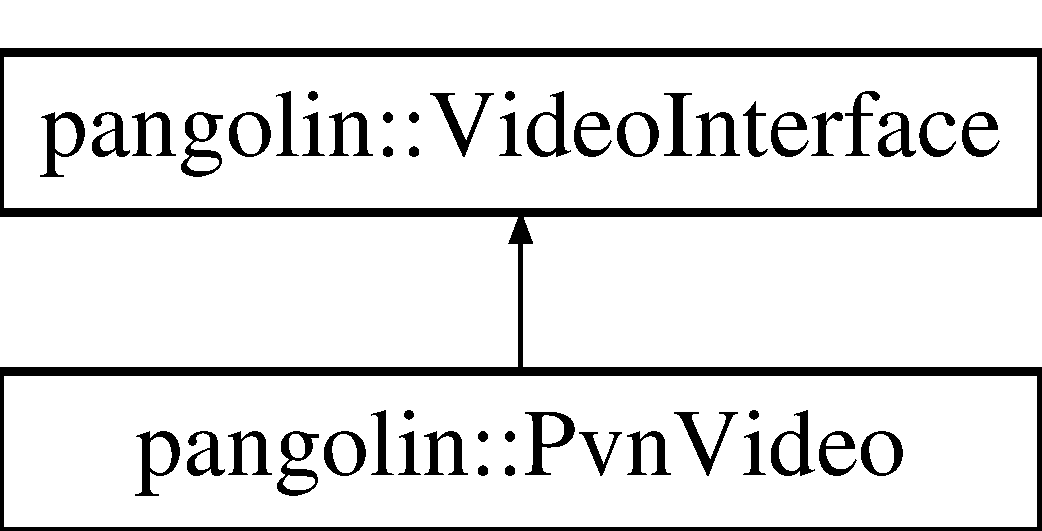
\includegraphics[height=2.000000cm]{classpangolin_1_1_pvn_video}
\end{center}
\end{figure}
\subsection*{Public Member Functions}
\begin{DoxyCompactItemize}
\item 
{\bfseries Pvn\+Video} (const std\+::string \&filename, bool realtime=false)\hypertarget{classpangolin_1_1_pvn_video_a400eea7ffd4dd3b470ddc184028d2c2b}{}\label{classpangolin_1_1_pvn_video_a400eea7ffd4dd3b470ddc184028d2c2b}

\item 
void \hyperlink{classpangolin_1_1_pvn_video_a9228cafe6aca4fb7464a6a1d1e6abc9d}{Start} ()\hypertarget{classpangolin_1_1_pvn_video_a9228cafe6aca4fb7464a6a1d1e6abc9d}{}\label{classpangolin_1_1_pvn_video_a9228cafe6aca4fb7464a6a1d1e6abc9d}

\begin{DoxyCompactList}\small\item\em Implement \hyperlink{structpangolin_1_1_video_input_a74a2e3e1b87c7cbf9de9bcb39e1df128}{Video\+Input\+::\+Start()} \end{DoxyCompactList}\item 
void \hyperlink{classpangolin_1_1_pvn_video_a62be1cc72d780a6fc96f603b8a1f3e35}{Stop} ()\hypertarget{classpangolin_1_1_pvn_video_a62be1cc72d780a6fc96f603b8a1f3e35}{}\label{classpangolin_1_1_pvn_video_a62be1cc72d780a6fc96f603b8a1f3e35}

\begin{DoxyCompactList}\small\item\em Implement \hyperlink{structpangolin_1_1_video_input_a8945f80194cc7ec9594db7f27e7d09b8}{Video\+Input\+::\+Stop()} \end{DoxyCompactList}\item 
size\+\_\+t \hyperlink{classpangolin_1_1_pvn_video_ae64b6281bae28d96d4972d21a9898797}{Size\+Bytes} () const \hypertarget{classpangolin_1_1_pvn_video_ae64b6281bae28d96d4972d21a9898797}{}\label{classpangolin_1_1_pvn_video_ae64b6281bae28d96d4972d21a9898797}

\begin{DoxyCompactList}\small\item\em Implement \hyperlink{structpangolin_1_1_video_input_a93cee5c33386973a2a51165e6bdcf40b}{Video\+Input\+::\+Size\+Bytes()} \end{DoxyCompactList}\item 
const std\+::vector$<$ \hyperlink{classpangolin_1_1_stream_info}{Stream\+Info} $>$ \& \hyperlink{classpangolin_1_1_pvn_video_a3c18009ef903c82fd4009ebc635020ae}{Streams} () const \hypertarget{classpangolin_1_1_pvn_video_a3c18009ef903c82fd4009ebc635020ae}{}\label{classpangolin_1_1_pvn_video_a3c18009ef903c82fd4009ebc635020ae}

\begin{DoxyCompactList}\small\item\em Implement \hyperlink{structpangolin_1_1_video_input_a9030d775d699c39ab7b7ba378c007c6a}{Video\+Input\+::\+Streams()} \end{DoxyCompactList}\item 
bool \hyperlink{classpangolin_1_1_pvn_video_abbe2e6f77a226c520fc40a79c443ba81}{Grab\+Next} (unsigned char $\ast$image, bool wait=true)\hypertarget{classpangolin_1_1_pvn_video_abbe2e6f77a226c520fc40a79c443ba81}{}\label{classpangolin_1_1_pvn_video_abbe2e6f77a226c520fc40a79c443ba81}

\begin{DoxyCompactList}\small\item\em Implement \hyperlink{structpangolin_1_1_video_input_ad3d8ff59c1ec4139320097e6e1111f32}{Video\+Input\+::\+Grab\+Next()} \end{DoxyCompactList}\item 
bool \hyperlink{classpangolin_1_1_pvn_video_abe3e1aa11b6ebb46842fae10cee2aa97}{Grab\+Newest} (unsigned char $\ast$image, bool wait=true)\hypertarget{classpangolin_1_1_pvn_video_abe3e1aa11b6ebb46842fae10cee2aa97}{}\label{classpangolin_1_1_pvn_video_abe3e1aa11b6ebb46842fae10cee2aa97}

\begin{DoxyCompactList}\small\item\em Implement \hyperlink{structpangolin_1_1_video_input_a4c8ac38e3c6a3f591663aeebf645e4c6}{Video\+Input\+::\+Grab\+Newest()} \end{DoxyCompactList}\end{DoxyCompactItemize}
\subsection*{Protected Member Functions}
\begin{DoxyCompactItemize}
\item 
void {\bfseries Read\+File\+Header} ()\hypertarget{classpangolin_1_1_pvn_video_af288a0b4427f1fafd7ade0619771591f}{}\label{classpangolin_1_1_pvn_video_af288a0b4427f1fafd7ade0619771591f}

\end{DoxyCompactItemize}
\subsection*{Protected Attributes}
\begin{DoxyCompactItemize}
\item 
int {\bfseries frames}\hypertarget{classpangolin_1_1_pvn_video_ac992b2df415c30dfc12f2a06b453c0d5}{}\label{classpangolin_1_1_pvn_video_ac992b2df415c30dfc12f2a06b453c0d5}

\item 
std\+::ifstream {\bfseries file}\hypertarget{classpangolin_1_1_pvn_video_a9176e1821e47a7aab33ebe1a77d1a00c}{}\label{classpangolin_1_1_pvn_video_a9176e1821e47a7aab33ebe1a77d1a00c}

\item 
std\+::vector$<$ \hyperlink{classpangolin_1_1_stream_info}{Stream\+Info} $>$ {\bfseries streams}\hypertarget{classpangolin_1_1_pvn_video_a843d63896c9aac7c0979f6b18e2bb750}{}\label{classpangolin_1_1_pvn_video_a843d63896c9aac7c0979f6b18e2bb750}

\item 
size\+\_\+t {\bfseries frame\+\_\+size\+\_\+bytes}\hypertarget{classpangolin_1_1_pvn_video_a6c20ee585d2b7b211fc0bb14d76e657e}{}\label{classpangolin_1_1_pvn_video_a6c20ee585d2b7b211fc0bb14d76e657e}

\item 
bool {\bfseries realtime}\hypertarget{classpangolin_1_1_pvn_video_a9fc8db20cd07ad434e7388370d1372e5}{}\label{classpangolin_1_1_pvn_video_a9fc8db20cd07ad434e7388370d1372e5}

\item 
pangolin\+::basetime {\bfseries frame\+\_\+interval}\hypertarget{classpangolin_1_1_pvn_video_a961ef0dba437cdd274c5539dd4198374}{}\label{classpangolin_1_1_pvn_video_a961ef0dba437cdd274c5539dd4198374}

\item 
pangolin\+::basetime {\bfseries last\+\_\+frame}\hypertarget{classpangolin_1_1_pvn_video_a8fca6c98411066d3e4cef526e8ad1d94}{}\label{classpangolin_1_1_pvn_video_a8fca6c98411066d3e4cef526e8ad1d94}

\end{DoxyCompactItemize}


The documentation for this class was generated from the following file\+:\begin{DoxyCompactItemize}
\item 
/home/gapo/meng/deps/pangolin/include/pangolin/video/drivers/pvn\+\_\+video.\+h\end{DoxyCompactItemize}

\hypertarget{classpangolin_1_1_py_interpreter}{}\section{pangolin\+:\+:Py\+Interpreter Class Reference}
\label{classpangolin_1_1_py_interpreter}\index{pangolin\+::\+Py\+Interpreter@{pangolin\+::\+Py\+Interpreter}}
Inheritance diagram for pangolin\+:\+:Py\+Interpreter\+:\begin{figure}[H]
\begin{center}
\leavevmode
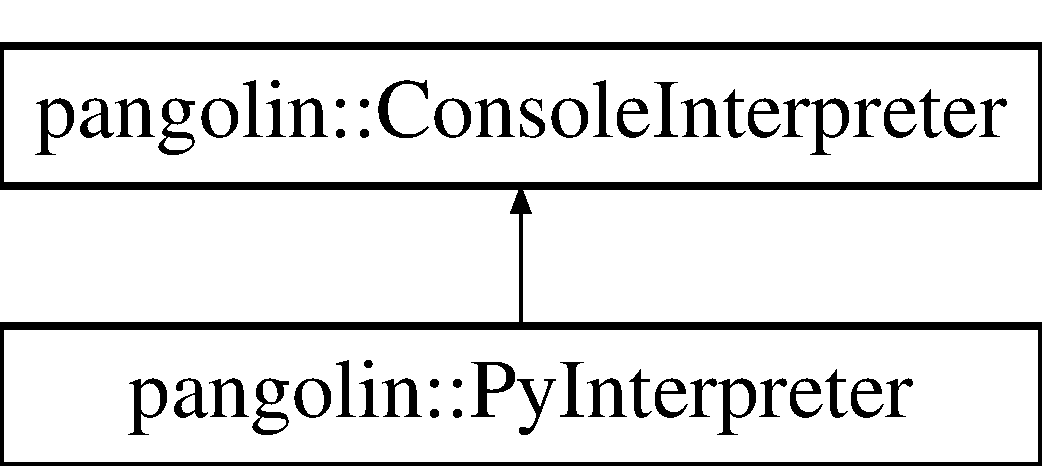
\includegraphics[height=2.000000cm]{classpangolin_1_1_py_interpreter}
\end{center}
\end{figure}
\subsection*{Public Member Functions}
\begin{DoxyCompactItemize}
\item 
void {\bfseries Push\+Command} (const std\+::string \&cmd) P\+A\+N\+G\+O\+L\+I\+N\+\_\+\+O\+V\+E\+R\+R\+I\+DE\hypertarget{classpangolin_1_1_py_interpreter_ac1428b8e6f708d84e68399f948e76a29}{}\label{classpangolin_1_1_py_interpreter_ac1428b8e6f708d84e68399f948e76a29}

\item 
bool {\bfseries Pull\+Line} (\hyperlink{classpangolin_1_1_console_line}{Console\+Line} \&line) P\+A\+N\+G\+O\+L\+I\+N\+\_\+\+O\+V\+E\+R\+R\+I\+DE\hypertarget{classpangolin_1_1_py_interpreter_ac91f101a3058d12c4f3cb211e8672f44}{}\label{classpangolin_1_1_py_interpreter_ac91f101a3058d12c4f3cb211e8672f44}

\item 
std\+::vector$<$ std\+::string $>$ {\bfseries Complete} (const std\+::string \&cmd, int max\+\_\+options) P\+A\+N\+G\+O\+L\+I\+N\+\_\+\+O\+V\+E\+R\+R\+I\+DE\hypertarget{classpangolin_1_1_py_interpreter_ae92fd82274bced062bfb6763e98ba813}{}\label{classpangolin_1_1_py_interpreter_ae92fd82274bced062bfb6763e98ba813}

\end{DoxyCompactItemize}
\subsection*{Static Public Member Functions}
\begin{DoxyCompactItemize}
\item 
static void {\bfseries Attach\+Prefix} (void $\ast$data, const std\+::string \&name, \hyperlink{classpangolin_1_1_var_value_generic}{Var\+Value\+Generic} \&var, bool brand\+\_\+new)\hypertarget{classpangolin_1_1_py_interpreter_ac53f11816bdc9c90c5d41484feb53c45}{}\label{classpangolin_1_1_py_interpreter_ac53f11816bdc9c90c5d41484feb53c45}

\end{DoxyCompactItemize}


The documentation for this class was generated from the following file\+:\begin{DoxyCompactItemize}
\item 
/home/gapo/meng/deps/pangolin/include/pangolin/python/Py\+Interpreter.\+h\end{DoxyCompactItemize}

\hypertarget{structpangolin_1_1_py_pango_i_o}{}\section{pangolin\+:\+:Py\+Pango\+IO Struct Reference}
\label{structpangolin_1_1_py_pango_i_o}\index{pangolin\+::\+Py\+Pango\+IO@{pangolin\+::\+Py\+Pango\+IO}}
\subsection*{Public Member Functions}
\begin{DoxyCompactItemize}
\item 
{\bfseries Py\+Pango\+IO} (Py\+Type\+Object $\ast$type, std\+::queue$<$ \hyperlink{classpangolin_1_1_console_line}{Console\+Line} $>$ \&line\+\_\+queue, Console\+Line\+Type line\+\_\+type)\hypertarget{structpangolin_1_1_py_pango_i_o_affd65261e9aa4ae6d79eca020836f219}{}\label{structpangolin_1_1_py_pango_i_o_affd65261e9aa4ae6d79eca020836f219}

\end{DoxyCompactItemize}
\subsection*{Static Public Member Functions}
\begin{DoxyCompactItemize}
\item 
static void {\bfseries Py\+\_\+dealloc} (\hyperlink{structpangolin_1_1_py_pango_i_o}{Py\+Pango\+IO} $\ast$self)\hypertarget{structpangolin_1_1_py_pango_i_o_a9beed7b822eed18bff7789e726434e55}{}\label{structpangolin_1_1_py_pango_i_o_a9beed7b822eed18bff7789e726434e55}

\item 
static Py\+Object $\ast$ {\bfseries Py\+\_\+new} (Py\+Type\+Object $\ast$, Py\+Object $\ast$, Py\+Object $\ast$)\hypertarget{structpangolin_1_1_py_pango_i_o_aaf2e562380f5731f38d6f36bd19b5105}{}\label{structpangolin_1_1_py_pango_i_o_aaf2e562380f5731f38d6f36bd19b5105}

\item 
static int {\bfseries Py\+\_\+init} (\hyperlink{structpangolin_1_1_py_pango_i_o}{Py\+Pango\+IO} $\ast$, Py\+Object $\ast$, Py\+Object $\ast$)\hypertarget{structpangolin_1_1_py_pango_i_o_a8b606fb56b0e5be4c5ec0f819b2d8ad3}{}\label{structpangolin_1_1_py_pango_i_o_a8b606fb56b0e5be4c5ec0f819b2d8ad3}

\item 
static Py\+Object $\ast$ {\bfseries Py\+\_\+getattr} (\hyperlink{structpangolin_1_1_py_pango_i_o}{Py\+Pango\+IO} $\ast$self, char $\ast$name)\hypertarget{structpangolin_1_1_py_pango_i_o_af649de2fe1ea485f0c02a49540302c3c}{}\label{structpangolin_1_1_py_pango_i_o_af649de2fe1ea485f0c02a49540302c3c}

\item 
static int {\bfseries Py\+\_\+setattr} (\hyperlink{structpangolin_1_1_py_pango_i_o}{Py\+Pango\+IO} $\ast$self, char $\ast$name, Py\+Object $\ast$val)\hypertarget{structpangolin_1_1_py_pango_i_o_a28dba892bbbf6213ee229a60b8d25c29}{}\label{structpangolin_1_1_py_pango_i_o_a28dba892bbbf6213ee229a60b8d25c29}

\item 
static Py\+Object $\ast$ {\bfseries Py\+\_\+write} (\hyperlink{structpangolin_1_1_py_pango_i_o}{Py\+Pango\+IO} $\ast$self, Py\+Object $\ast$args)\hypertarget{structpangolin_1_1_py_pango_i_o_a4a53751f40b84ed440145244025399c9}{}\label{structpangolin_1_1_py_pango_i_o_a4a53751f40b84ed440145244025399c9}

\end{DoxyCompactItemize}
\subsection*{Public Attributes}
\begin{DoxyCompactItemize}
\item 
std\+::string {\bfseries buffer}\hypertarget{structpangolin_1_1_py_pango_i_o_aa9b5f727d226c9c9ef6867e92c610bb4}{}\label{structpangolin_1_1_py_pango_i_o_aa9b5f727d226c9c9ef6867e92c610bb4}

\item 
std\+::queue$<$ \hyperlink{classpangolin_1_1_console_line}{Console\+Line} $>$ \& {\bfseries line\+\_\+queue}\hypertarget{structpangolin_1_1_py_pango_i_o_a20c29d09809db19ce2d83ef461fdef93}{}\label{structpangolin_1_1_py_pango_i_o_a20c29d09809db19ce2d83ef461fdef93}

\item 
Console\+Line\+Type {\bfseries line\+\_\+type}\hypertarget{structpangolin_1_1_py_pango_i_o_a05d6e69ccbc944325b59f087980e4824}{}\label{structpangolin_1_1_py_pango_i_o_a05d6e69ccbc944325b59f087980e4824}

\end{DoxyCompactItemize}
\subsection*{Static Public Attributes}
\begin{DoxyCompactItemize}
\item 
static Py\+Object\+\_\+\+H\+E\+AD Py\+Type\+Object {\bfseries Py\+\_\+type}\hypertarget{structpangolin_1_1_py_pango_i_o_a7aae650a6e75ee086dc50cfd4bb76257}{}\label{structpangolin_1_1_py_pango_i_o_a7aae650a6e75ee086dc50cfd4bb76257}

\item 
static Py\+Method\+Def {\bfseries Py\+\_\+methods} \mbox{[}$\,$\mbox{]}
\end{DoxyCompactItemize}


\subsection{Member Data Documentation}
\index{pangolin\+::\+Py\+Pango\+IO@{pangolin\+::\+Py\+Pango\+IO}!Py\+\_\+methods@{Py\+\_\+methods}}
\index{Py\+\_\+methods@{Py\+\_\+methods}!pangolin\+::\+Py\+Pango\+IO@{pangolin\+::\+Py\+Pango\+IO}}
\subsubsection[{\texorpdfstring{Py\+\_\+methods}{Py_methods}}]{\setlength{\rightskip}{0pt plus 5cm}Py\+Method\+Def pangolin\+::\+Py\+Pango\+I\+O\+::\+Py\+\_\+methods\hspace{0.3cm}{\ttfamily [static]}}\hypertarget{structpangolin_1_1_py_pango_i_o_a16ce452a74d6cda7903a0b3f6a7e6bb0}{}\label{structpangolin_1_1_py_pango_i_o_a16ce452a74d6cda7903a0b3f6a7e6bb0}
{\bfseries Initial value\+:}
\begin{DoxyCode}
= \{
    \{\textcolor{stringliteral}{"write"}, (PyCFunction)PyPangoIO::Py\_write, METH\_VARARGS, \textcolor{stringliteral}{"Write to console"} \},
    \{NULL\}
\}
\end{DoxyCode}


The documentation for this struct was generated from the following file\+:\begin{DoxyCompactItemize}
\item 
/home/gapo/meng/deps/pangolin/include/pangolin/python/Py\+Pango\+I\+O.\+h\end{DoxyCompactItemize}

\hypertarget{classpangolin_1_1_py_unique_obj}{}\section{pangolin\+:\+:Py\+Unique\+Obj Class Reference}
\label{classpangolin_1_1_py_unique_obj}\index{pangolin\+::\+Py\+Unique\+Obj@{pangolin\+::\+Py\+Unique\+Obj}}


Class represents a reference counted Python\+Object.  




{\ttfamily \#include $<$Py\+Unique\+Obj.\+h$>$}

\subsection*{Public Member Functions}
\begin{DoxyCompactItemize}
\item 
\hyperlink{classpangolin_1_1_py_unique_obj_abfaa0af0151225e61c271d3bd56870ed}{Py\+Unique\+Obj} (Py\+Object $\ast$obj)\hypertarget{classpangolin_1_1_py_unique_obj_abfaa0af0151225e61c271d3bd56870ed}{}\label{classpangolin_1_1_py_unique_obj_abfaa0af0151225e61c271d3bd56870ed}

\begin{DoxyCompactList}\small\item\em Assumption\+: Python\+Object has already been appropriately I\+N\+C\+R\+EF\textquotesingle{}d. \end{DoxyCompactList}\item 
{\bfseries Py\+Unique\+Obj} (const \hyperlink{classpangolin_1_1_py_unique_obj}{Py\+Unique\+Obj} \&other)\hypertarget{classpangolin_1_1_py_unique_obj_a5ec1ea99743b1665a284c8aa15a223eb}{}\label{classpangolin_1_1_py_unique_obj_a5ec1ea99743b1665a284c8aa15a223eb}

\item 
void {\bfseries operator=} (Py\+Object $\ast$obj)\hypertarget{classpangolin_1_1_py_unique_obj_a4a06ce387418f7dc023ca507a929c8fc}{}\label{classpangolin_1_1_py_unique_obj_a4a06ce387418f7dc023ca507a929c8fc}

\item 
void {\bfseries Release} ()\hypertarget{classpangolin_1_1_py_unique_obj_a4a3da785bbf7d591db2ae38629b12b7e}{}\label{classpangolin_1_1_py_unique_obj_a4a3da785bbf7d591db2ae38629b12b7e}

\item 
Py\+Object $\ast$ {\bfseries operator$\ast$} ()\hypertarget{classpangolin_1_1_py_unique_obj_a836d7dc785df9cb6363c26e2dbe53975}{}\label{classpangolin_1_1_py_unique_obj_a836d7dc785df9cb6363c26e2dbe53975}

\item 
{\bfseries operator Py\+Object $\ast$} ()\hypertarget{classpangolin_1_1_py_unique_obj_ac2663319ceff9bda46c106e67eb82bc3}{}\label{classpangolin_1_1_py_unique_obj_ac2663319ceff9bda46c106e67eb82bc3}

\end{DoxyCompactItemize}


\subsection{Detailed Description}
Class represents a reference counted Python\+Object. 

Python\+Object is appropriately Py\+\_\+\+I\+N\+C\+R\+EF\textquotesingle{}d and Py\+\_\+\+D\+E\+C\+R\+EF\textquotesingle{}d 

The documentation for this class was generated from the following file\+:\begin{DoxyCompactItemize}
\item 
/home/gapo/meng/deps/pangolin/include/pangolin/python/Py\+Unique\+Obj.\+h\end{DoxyCompactItemize}

\hypertarget{structpangolin_1_1_py_var}{}\section{pangolin\+:\+:Py\+Var Struct Reference}
\label{structpangolin_1_1_py_var}\index{pangolin\+::\+Py\+Var@{pangolin\+::\+Py\+Var}}
\subsection*{Public Member Functions}
\begin{DoxyCompactItemize}
\item 
Py\+Object\+\_\+\+H\+E\+AD {\bfseries Py\+Var} (Py\+Type\+Object $\ast$type)\hypertarget{structpangolin_1_1_py_var_aa473b639c7e0f8eae7a5231433fb0a2c}{}\label{structpangolin_1_1_py_var_aa473b639c7e0f8eae7a5231433fb0a2c}

\end{DoxyCompactItemize}
\subsection*{Static Public Member Functions}
\begin{DoxyCompactItemize}
\item 
static void {\bfseries Py\+\_\+dealloc} (\hyperlink{structpangolin_1_1_py_var}{Py\+Var} $\ast$self)\hypertarget{structpangolin_1_1_py_var_a4eb34b521908b2fc6475cb995de295de}{}\label{structpangolin_1_1_py_var_a4eb34b521908b2fc6475cb995de295de}

\item 
static Py\+Object $\ast$ {\bfseries Py\+\_\+new} (Py\+Type\+Object $\ast$type, Py\+Object $\ast$args, Py\+Object $\ast$kwds)\hypertarget{structpangolin_1_1_py_var_aa6170501c16da5a331e6fb45fcb1d823}{}\label{structpangolin_1_1_py_var_aa6170501c16da5a331e6fb45fcb1d823}

\item 
static int {\bfseries Py\+\_\+init} (\hyperlink{structpangolin_1_1_py_var}{Py\+Var} $\ast$self, Py\+Object $\ast$args, Py\+Object $\ast$kwds)\hypertarget{structpangolin_1_1_py_var_a363ce6897c5fb8c3cfed688e12780a70}{}\label{structpangolin_1_1_py_var_a363ce6897c5fb8c3cfed688e12780a70}

\item 
static Py\+Object $\ast$ {\bfseries Py\+\_\+getattr} (\hyperlink{structpangolin_1_1_py_var}{Py\+Var} $\ast$self, char $\ast$name)\hypertarget{structpangolin_1_1_py_var_a5aac21ee4d27de2b7de87d5b8d37f0e9}{}\label{structpangolin_1_1_py_var_a5aac21ee4d27de2b7de87d5b8d37f0e9}

\item 
static int {\bfseries Py\+\_\+setattr} (\hyperlink{structpangolin_1_1_py_var}{Py\+Var} $\ast$self, char $\ast$name, Py\+Object $\ast$val)\hypertarget{structpangolin_1_1_py_var_a09ac9a993882c98728fafcdf094ee6f5}{}\label{structpangolin_1_1_py_var_a09ac9a993882c98728fafcdf094ee6f5}

\end{DoxyCompactItemize}
\subsection*{Public Attributes}
\begin{DoxyCompactItemize}
\item 
std\+::string {\bfseries ns}\hypertarget{structpangolin_1_1_py_var_afe67c98bf7b61dab11a2c3950fe072e4}{}\label{structpangolin_1_1_py_var_afe67c98bf7b61dab11a2c3950fe072e4}

\end{DoxyCompactItemize}
\subsection*{Static Public Attributes}
\begin{DoxyCompactItemize}
\item 
static Py\+Type\+Object {\bfseries Py\+\_\+type}\hypertarget{structpangolin_1_1_py_var_a3b7bbb244a43b6304ee3b841ba2ae054}{}\label{structpangolin_1_1_py_var_a3b7bbb244a43b6304ee3b841ba2ae054}

\end{DoxyCompactItemize}


The documentation for this struct was generated from the following file\+:\begin{DoxyCompactItemize}
\item 
/home/gapo/meng/deps/pangolin/include/pangolin/python/Py\+Var.\+h\end{DoxyCompactItemize}

\hypertarget{structpangolin_1_1_range}{}\section{pangolin\+:\+:Range$<$ T $>$ Struct Template Reference}
\label{structpangolin_1_1_range}\index{pangolin\+::\+Range$<$ T $>$@{pangolin\+::\+Range$<$ T $>$}}
\subsection*{Public Member Functions}
\begin{DoxyCompactItemize}
\item 
{\bfseries Range} (T rmin, T rmax)\hypertarget{structpangolin_1_1_range_a68ab0b6208d5afbf3ef72f4b3a5d3340}{}\label{structpangolin_1_1_range_a68ab0b6208d5afbf3ef72f4b3a5d3340}

\item 
\hyperlink{structpangolin_1_1_range}{Range} {\bfseries operator+} (T v)\hypertarget{structpangolin_1_1_range_ae3b7cd34f2df378e8ee58291786fd00c}{}\label{structpangolin_1_1_range_ae3b7cd34f2df378e8ee58291786fd00c}

\item 
\hyperlink{structpangolin_1_1_range}{Range} {\bfseries operator-\/} (T v)\hypertarget{structpangolin_1_1_range_a07c65c99f9fd1ed257efaab345beb058}{}\label{structpangolin_1_1_range_a07c65c99f9fd1ed257efaab345beb058}

\item 
\hyperlink{structpangolin_1_1_range}{Range} \& {\bfseries operator+=} (T v)\hypertarget{structpangolin_1_1_range_a9afee6e4374ca1e287a0da8664442b62}{}\label{structpangolin_1_1_range_a9afee6e4374ca1e287a0da8664442b62}

\item 
\hyperlink{structpangolin_1_1_range}{Range} \& {\bfseries operator-\/=} (T v)\hypertarget{structpangolin_1_1_range_a47086ff33fb7a1714a03a97562868e68}{}\label{structpangolin_1_1_range_a47086ff33fb7a1714a03a97562868e68}

\item 
\hyperlink{structpangolin_1_1_range}{Range} \& {\bfseries operator$\ast$=} (T v)\hypertarget{structpangolin_1_1_range_ab37236fb30c01e03ffaeb6e0224091c9}{}\label{structpangolin_1_1_range_ab37236fb30c01e03ffaeb6e0224091c9}

\item 
\hyperlink{structpangolin_1_1_range}{Range} \& {\bfseries operator/=} (T v)\hypertarget{structpangolin_1_1_range_af32494456c60c208e3dc80461af9d512}{}\label{structpangolin_1_1_range_af32494456c60c208e3dc80461af9d512}

\item 
\hyperlink{structpangolin_1_1_range}{Range} \& {\bfseries operator+=} (const \hyperlink{structpangolin_1_1_range}{Range} \&o)\hypertarget{structpangolin_1_1_range_ac9648234982c25b263acc282535d9986}{}\label{structpangolin_1_1_range_ac9648234982c25b263acc282535d9986}

\item 
\hyperlink{structpangolin_1_1_range}{Range} \& {\bfseries operator-\/=} (const \hyperlink{structpangolin_1_1_range}{Range} \&o)\hypertarget{structpangolin_1_1_range_a1094325106f0da7becdddb53326ee737}{}\label{structpangolin_1_1_range_a1094325106f0da7becdddb53326ee737}

\item 
\hyperlink{structpangolin_1_1_range}{Range} {\bfseries operator+} (const \hyperlink{structpangolin_1_1_range}{Range} \&o) const \hypertarget{structpangolin_1_1_range_aaadd38585055ec532c1e0bbfce99dff6}{}\label{structpangolin_1_1_range_aaadd38585055ec532c1e0bbfce99dff6}

\item 
\hyperlink{structpangolin_1_1_range}{Range} {\bfseries operator-\/} (const \hyperlink{structpangolin_1_1_range}{Range} \&o) const \hypertarget{structpangolin_1_1_range_a77c3cac8a9abd2b72ddbf0eec791341d}{}\label{structpangolin_1_1_range_a77c3cac8a9abd2b72ddbf0eec791341d}

\item 
\hyperlink{structpangolin_1_1_range}{Range} {\bfseries operator$\ast$} (float s) const \hypertarget{structpangolin_1_1_range_aa578f99d69ee414485ca17d5ed6bfb02}{}\label{structpangolin_1_1_range_aa578f99d69ee414485ca17d5ed6bfb02}

\item 
T {\bfseries Size} () const \hypertarget{structpangolin_1_1_range_a1726b483eb1a07ef70bb3677301f58dc}{}\label{structpangolin_1_1_range_a1726b483eb1a07ef70bb3677301f58dc}

\item 
T {\bfseries Abs\+Size} () const \hypertarget{structpangolin_1_1_range_a76d177022bd4c18aad57f78d278f0be2}{}\label{structpangolin_1_1_range_a76d177022bd4c18aad57f78d278f0be2}

\item 
T {\bfseries Mid} () const \hypertarget{structpangolin_1_1_range_a5d89e629b03d26a16164f3bdddcc5ed0}{}\label{structpangolin_1_1_range_a5d89e629b03d26a16164f3bdddcc5ed0}

\item 
void {\bfseries Scale} (float s, float center=0.\+0f)\hypertarget{structpangolin_1_1_range_a1d5f22742fae07ad1f14b17b801f07fb}{}\label{structpangolin_1_1_range_a1d5f22742fae07ad1f14b17b801f07fb}

\item 
void {\bfseries Insert} (T v)\hypertarget{structpangolin_1_1_range_a35b7256dfcdf8ecfbd5b71b46181e7cc}{}\label{structpangolin_1_1_range_a35b7256dfcdf8ecfbd5b71b46181e7cc}

\item 
void {\bfseries Clamp} (T vmin, T vmax)\hypertarget{structpangolin_1_1_range_afb2b0897bb07ceff15bb9f8ae469d4b0}{}\label{structpangolin_1_1_range_afb2b0897bb07ceff15bb9f8ae469d4b0}

\item 
void {\bfseries Clamp} (const \hyperlink{structpangolin_1_1_range}{Range} \&o)\hypertarget{structpangolin_1_1_range_a3b3bf7b1f9b247c06e1e3632454ae1af}{}\label{structpangolin_1_1_range_a3b3bf7b1f9b247c06e1e3632454ae1af}

\item 
void {\bfseries Clear} ()\hypertarget{structpangolin_1_1_range_ad8b61e9ea4c7dd05b4e361e971c0e364}{}\label{structpangolin_1_1_range_ad8b61e9ea4c7dd05b4e361e971c0e364}

\item 
{\footnotesize template$<$typename To $>$ }\\\hyperlink{structpangolin_1_1_range}{Range}$<$ To $>$ {\bfseries Cast} ()\hypertarget{structpangolin_1_1_range_aa9f8526131baf0ce0cce59a6542b6948}{}\label{structpangolin_1_1_range_aa9f8526131baf0ce0cce59a6542b6948}

\end{DoxyCompactItemize}
\subsection*{Public Attributes}
\begin{DoxyCompactItemize}
\item 
T {\bfseries min}\hypertarget{structpangolin_1_1_range_af490e89dcf64b2afec94a823069b14cb}{}\label{structpangolin_1_1_range_af490e89dcf64b2afec94a823069b14cb}

\item 
T {\bfseries max}\hypertarget{structpangolin_1_1_range_ac81b20be20857a8f5e58689f382c06d7}{}\label{structpangolin_1_1_range_ac81b20be20857a8f5e58689f382c06d7}

\end{DoxyCompactItemize}


The documentation for this struct was generated from the following file\+:\begin{DoxyCompactItemize}
\item 
/home/gapo/meng/deps/pangolin/include/pangolin/plot/range.\+h\end{DoxyCompactItemize}

\hypertarget{structpangolin_1_1_depth_sense_video_1_1_sensor_config}{}\section{pangolin\+:\+:Depth\+Sense\+Video\+:\+:Sensor\+Config Struct Reference}
\label{structpangolin_1_1_depth_sense_video_1_1_sensor_config}\index{pangolin\+::\+Depth\+Sense\+Video\+::\+Sensor\+Config@{pangolin\+::\+Depth\+Sense\+Video\+::\+Sensor\+Config}}
\subsection*{Public Attributes}
\begin{DoxyCompactItemize}
\item 
Depth\+Sense\+Sensor\+Type {\bfseries type}\hypertarget{structpangolin_1_1_depth_sense_video_1_1_sensor_config_ac4c33357c308ccc3c16fff29bcfa0675}{}\label{structpangolin_1_1_depth_sense_video_1_1_sensor_config_ac4c33357c308ccc3c16fff29bcfa0675}

\item 
\hyperlink{structpangolin_1_1_image_dim}{Image\+Dim} {\bfseries dim}\hypertarget{structpangolin_1_1_depth_sense_video_1_1_sensor_config_afca75db803ad81a151910b4d637e08e7}{}\label{structpangolin_1_1_depth_sense_video_1_1_sensor_config_afca75db803ad81a151910b4d637e08e7}

\item 
unsigned int {\bfseries fps}\hypertarget{structpangolin_1_1_depth_sense_video_1_1_sensor_config_a2093c03e53ccfe4a48557bf3a3918a72}{}\label{structpangolin_1_1_depth_sense_video_1_1_sensor_config_a2093c03e53ccfe4a48557bf3a3918a72}

\end{DoxyCompactItemize}


The documentation for this struct was generated from the following file\+:\begin{DoxyCompactItemize}
\item 
/home/gapo/meng/deps/pangolin/include/pangolin/video/drivers/depthsense.\+h\end{DoxyCompactItemize}

\hypertarget{structpangolin_1_1_set_var_functor}{}\section{pangolin\+:\+:Set\+Var\+Functor$<$ T $>$ Struct Template Reference}
\label{structpangolin_1_1_set_var_functor}\index{pangolin\+::\+Set\+Var\+Functor$<$ T $>$@{pangolin\+::\+Set\+Var\+Functor$<$ T $>$}}
\subsection*{Public Member Functions}
\begin{DoxyCompactItemize}
\item 
{\bfseries Set\+Var\+Functor} (const std\+::string \&name, T val)\hypertarget{structpangolin_1_1_set_var_functor_a784b09d37ebc818ed1168deec5371eef}{}\label{structpangolin_1_1_set_var_functor_a784b09d37ebc818ed1168deec5371eef}

\item 
void {\bfseries operator()} ()\hypertarget{structpangolin_1_1_set_var_functor_a7f24b53dbb8f9a2ba159b4ea914c78a5}{}\label{structpangolin_1_1_set_var_functor_a7f24b53dbb8f9a2ba159b4ea914c78a5}

\end{DoxyCompactItemize}
\subsection*{Public Attributes}
\begin{DoxyCompactItemize}
\item 
std\+::string {\bfseries var\+Name}\hypertarget{structpangolin_1_1_set_var_functor_a47e6732ba66d6c761f26262253c0f421}{}\label{structpangolin_1_1_set_var_functor_a47e6732ba66d6c761f26262253c0f421}

\item 
T {\bfseries set\+Val}\hypertarget{structpangolin_1_1_set_var_functor_acf385bff6fc6b60d208c24a7ba58678f}{}\label{structpangolin_1_1_set_var_functor_acf385bff6fc6b60d208c24a7ba58678f}

\end{DoxyCompactItemize}


The documentation for this struct was generated from the following file\+:\begin{DoxyCompactItemize}
\item 
/home/gapo/meng/deps/pangolin/include/pangolin/var/varextra.\+h\end{DoxyCompactItemize}

\hypertarget{classpangolin_1_1_shift_video}{}\section{pangolin\+:\+:Shift\+Video Class Reference}
\label{classpangolin_1_1_shift_video}\index{pangolin\+::\+Shift\+Video@{pangolin\+::\+Shift\+Video}}
Inheritance diagram for pangolin\+:\+:Shift\+Video\+:\begin{figure}[H]
\begin{center}
\leavevmode
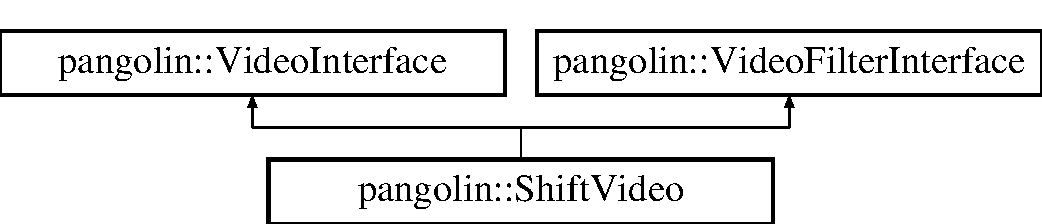
\includegraphics[height=2.000000cm]{classpangolin_1_1_shift_video}
\end{center}
\end{figure}
\subsection*{Public Member Functions}
\begin{DoxyCompactItemize}
\item 
{\bfseries Shift\+Video} (\hyperlink{structpangolin_1_1_video_interface}{Video\+Interface} $\ast$videoin, \hyperlink{structpangolin_1_1_video_pixel_format}{Video\+Pixel\+Format} new\+\_\+fmt, int shift\+\_\+right\+\_\+bits=0, unsigned int mask=0x\+F\+F\+F\+F)\hypertarget{classpangolin_1_1_shift_video_a8ad45176015a35aed0e50481c2badce4}{}\label{classpangolin_1_1_shift_video_a8ad45176015a35aed0e50481c2badce4}

\item 
void \hyperlink{classpangolin_1_1_shift_video_abd1b69a437aed53dbcf6e064a15d82a3}{Start} ()\hypertarget{classpangolin_1_1_shift_video_abd1b69a437aed53dbcf6e064a15d82a3}{}\label{classpangolin_1_1_shift_video_abd1b69a437aed53dbcf6e064a15d82a3}

\begin{DoxyCompactList}\small\item\em Implement \hyperlink{structpangolin_1_1_video_input_a74a2e3e1b87c7cbf9de9bcb39e1df128}{Video\+Input\+::\+Start()} \end{DoxyCompactList}\item 
void \hyperlink{classpangolin_1_1_shift_video_a403662f0304427ea8ca047e7d02fb369}{Stop} ()\hypertarget{classpangolin_1_1_shift_video_a403662f0304427ea8ca047e7d02fb369}{}\label{classpangolin_1_1_shift_video_a403662f0304427ea8ca047e7d02fb369}

\begin{DoxyCompactList}\small\item\em Implement \hyperlink{structpangolin_1_1_video_input_a8945f80194cc7ec9594db7f27e7d09b8}{Video\+Input\+::\+Stop()} \end{DoxyCompactList}\item 
size\+\_\+t \hyperlink{classpangolin_1_1_shift_video_aaaf42a6603580c8376769d144945df0e}{Size\+Bytes} () const \hypertarget{classpangolin_1_1_shift_video_aaaf42a6603580c8376769d144945df0e}{}\label{classpangolin_1_1_shift_video_aaaf42a6603580c8376769d144945df0e}

\begin{DoxyCompactList}\small\item\em Implement \hyperlink{structpangolin_1_1_video_input_a93cee5c33386973a2a51165e6bdcf40b}{Video\+Input\+::\+Size\+Bytes()} \end{DoxyCompactList}\item 
const std\+::vector$<$ \hyperlink{classpangolin_1_1_stream_info}{Stream\+Info} $>$ \& \hyperlink{classpangolin_1_1_shift_video_a63488eb65d208cc1b05a9d4baf3d6058}{Streams} () const \hypertarget{classpangolin_1_1_shift_video_a63488eb65d208cc1b05a9d4baf3d6058}{}\label{classpangolin_1_1_shift_video_a63488eb65d208cc1b05a9d4baf3d6058}

\begin{DoxyCompactList}\small\item\em Implement \hyperlink{structpangolin_1_1_video_input_a9030d775d699c39ab7b7ba378c007c6a}{Video\+Input\+::\+Streams()} \end{DoxyCompactList}\item 
bool \hyperlink{classpangolin_1_1_shift_video_a67e43e271b0cef25e74c236580ebdd99}{Grab\+Next} (unsigned char $\ast$image, bool wait=true)\hypertarget{classpangolin_1_1_shift_video_a67e43e271b0cef25e74c236580ebdd99}{}\label{classpangolin_1_1_shift_video_a67e43e271b0cef25e74c236580ebdd99}

\begin{DoxyCompactList}\small\item\em Implement \hyperlink{structpangolin_1_1_video_input_ad3d8ff59c1ec4139320097e6e1111f32}{Video\+Input\+::\+Grab\+Next()} \end{DoxyCompactList}\item 
bool \hyperlink{classpangolin_1_1_shift_video_a6a892441163b80351fcaac011964cf6c}{Grab\+Newest} (unsigned char $\ast$image, bool wait=true)\hypertarget{classpangolin_1_1_shift_video_a6a892441163b80351fcaac011964cf6c}{}\label{classpangolin_1_1_shift_video_a6a892441163b80351fcaac011964cf6c}

\begin{DoxyCompactList}\small\item\em Implement \hyperlink{structpangolin_1_1_video_input_a4c8ac38e3c6a3f591663aeebf645e4c6}{Video\+Input\+::\+Grab\+Newest()} \end{DoxyCompactList}\item 
std\+::vector$<$ \hyperlink{structpangolin_1_1_video_interface}{Video\+Interface} $\ast$ $>$ \& {\bfseries Input\+Streams} ()\hypertarget{classpangolin_1_1_shift_video_a47fb5b8af22e7c95f68e425c53212a11}{}\label{classpangolin_1_1_shift_video_a47fb5b8af22e7c95f68e425c53212a11}

\end{DoxyCompactItemize}
\subsection*{Protected Attributes}
\begin{DoxyCompactItemize}
\item 
std\+::vector$<$ \hyperlink{structpangolin_1_1_video_interface}{Video\+Interface} $\ast$ $>$ {\bfseries videoin}\hypertarget{classpangolin_1_1_shift_video_ab4395c3eb68c486d8a8fed8195a02aec}{}\label{classpangolin_1_1_shift_video_ab4395c3eb68c486d8a8fed8195a02aec}

\item 
std\+::vector$<$ \hyperlink{classpangolin_1_1_stream_info}{Stream\+Info} $>$ {\bfseries streams}\hypertarget{classpangolin_1_1_shift_video_a1070e30e0b218fa754cd28cd61b926c3}{}\label{classpangolin_1_1_shift_video_a1070e30e0b218fa754cd28cd61b926c3}

\item 
size\+\_\+t {\bfseries size\+\_\+bytes}\hypertarget{classpangolin_1_1_shift_video_a43d1b3eefb55556e3e02b56ad0538ce9}{}\label{classpangolin_1_1_shift_video_a43d1b3eefb55556e3e02b56ad0538ce9}

\item 
unsigned char $\ast$ {\bfseries buffer}\hypertarget{classpangolin_1_1_shift_video_ab6c0151499a02c64253c601a37bb0008}{}\label{classpangolin_1_1_shift_video_ab6c0151499a02c64253c601a37bb0008}

\item 
int {\bfseries shift\+\_\+right\+\_\+bits}\hypertarget{classpangolin_1_1_shift_video_a9fc55d6a38c76797928fea95a6694f95}{}\label{classpangolin_1_1_shift_video_a9fc55d6a38c76797928fea95a6694f95}

\item 
unsigned int {\bfseries mask}\hypertarget{classpangolin_1_1_shift_video_a2ac01689d4cac5e8db54c0a220a3b8ea}{}\label{classpangolin_1_1_shift_video_a2ac01689d4cac5e8db54c0a220a3b8ea}

\end{DoxyCompactItemize}


The documentation for this class was generated from the following file\+:\begin{DoxyCompactItemize}
\item 
/home/gapo/meng/deps/pangolin/include/pangolin/video/drivers/shift.\+h\end{DoxyCompactItemize}

\hypertarget{structpangolin_1_1_slider}{}\section{pangolin\+:\+:Slider Struct Reference}
\label{structpangolin_1_1_slider}\index{pangolin\+::\+Slider@{pangolin\+::\+Slider}}
Inheritance diagram for pangolin\+:\+:Slider\+:\begin{figure}[H]
\begin{center}
\leavevmode
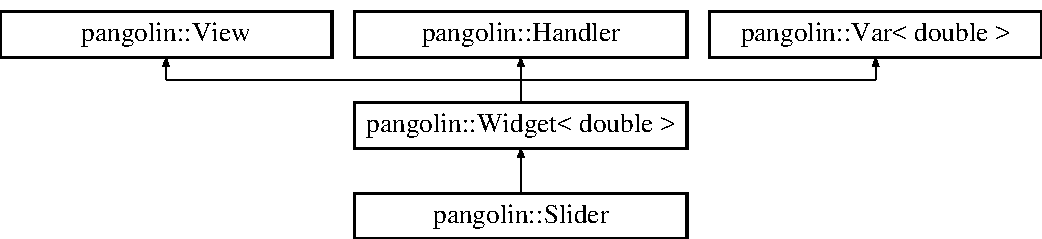
\includegraphics[height=3.000000cm]{structpangolin_1_1_slider}
\end{center}
\end{figure}
\subsection*{Public Member Functions}
\begin{DoxyCompactItemize}
\item 
{\bfseries Slider} (std\+::string title, \hyperlink{classpangolin_1_1_var_value_generic}{Var\+Value\+Generic} \&tv)\hypertarget{structpangolin_1_1_slider_af26204a5865981cbcd99d275ca7b7d8f}{}\label{structpangolin_1_1_slider_af26204a5865981cbcd99d275ca7b7d8f}

\item 
void {\bfseries Mouse} (\hyperlink{structpangolin_1_1_view}{View} \&, Mouse\+Button button, int x, int y, bool pressed, int mouse\+\_\+state)\hypertarget{structpangolin_1_1_slider_a2897c9859dd1cbd5c7594125b8f7cf2a}{}\label{structpangolin_1_1_slider_a2897c9859dd1cbd5c7594125b8f7cf2a}

\item 
void {\bfseries Mouse\+Motion} (\hyperlink{structpangolin_1_1_view}{View} \&, int x, int y, int mouse\+\_\+state)\hypertarget{structpangolin_1_1_slider_a4b500c84249d23baa7b8ba41cb4d572c}{}\label{structpangolin_1_1_slider_a4b500c84249d23baa7b8ba41cb4d572c}

\item 
void {\bfseries Keyboard} (\hyperlink{structpangolin_1_1_view}{View} \&, unsigned char key, int x, int y, bool pressed)\hypertarget{structpangolin_1_1_slider_a0ff85db665a2a794f8a4047f12f4e371}{}\label{structpangolin_1_1_slider_a0ff85db665a2a794f8a4047f12f4e371}

\item 
void \hyperlink{structpangolin_1_1_slider_a53b5643f938eebc26db70f4f85e07bd2}{Render} ()
\begin{DoxyCompactList}\small\item\em Perform any automatic rendering for this \hyperlink{structpangolin_1_1_view}{View}. \end{DoxyCompactList}\item 
void \hyperlink{structpangolin_1_1_slider_a6b8366d0c9c49ee4e6361a8e4215b42a}{Resize\+Children} ()\hypertarget{structpangolin_1_1_slider_a6b8366d0c9c49ee4e6361a8e4215b42a}{}\label{structpangolin_1_1_slider_a6b8366d0c9c49ee4e6361a8e4215b42a}

\begin{DoxyCompactList}\small\item\em Instruct all children to resize. \end{DoxyCompactList}\end{DoxyCompactItemize}
\subsection*{Public Attributes}
\begin{DoxyCompactItemize}
\item 
\hyperlink{classpangolin_1_1_gl_text}{Gl\+Text} {\bfseries gltext}\hypertarget{structpangolin_1_1_slider_af7907379d750713772a88cddb26bd939}{}\label{structpangolin_1_1_slider_af7907379d750713772a88cddb26bd939}

\item 
G\+Lfloat {\bfseries raster} \mbox{[}2\mbox{]}\hypertarget{structpangolin_1_1_slider_ad693dcacf42645686df847645b1c42d2}{}\label{structpangolin_1_1_slider_ad693dcacf42645686df847645b1c42d2}

\item 
bool {\bfseries lock\+\_\+bounds}\hypertarget{structpangolin_1_1_slider_a3a6dc41e6c84ddf37bda086df90853ea}{}\label{structpangolin_1_1_slider_a3a6dc41e6c84ddf37bda086df90853ea}

\item 
bool {\bfseries logscale}\hypertarget{structpangolin_1_1_slider_adeedb755d8a6c636e3caf7770bbb0c5f}{}\label{structpangolin_1_1_slider_adeedb755d8a6c636e3caf7770bbb0c5f}

\end{DoxyCompactItemize}
\subsection*{Additional Inherited Members}


\subsection{Member Function Documentation}
\index{pangolin\+::\+Slider@{pangolin\+::\+Slider}!Render@{Render}}
\index{Render@{Render}!pangolin\+::\+Slider@{pangolin\+::\+Slider}}
\subsubsection[{\texorpdfstring{Render()}{Render()}}]{\setlength{\rightskip}{0pt plus 5cm}void pangolin\+::\+Slider\+::\+Render (
\begin{DoxyParamCaption}
{}
\end{DoxyParamCaption}
)\hspace{0.3cm}{\ttfamily [virtual]}}\hypertarget{structpangolin_1_1_slider_a53b5643f938eebc26db70f4f85e07bd2}{}\label{structpangolin_1_1_slider_a53b5643f938eebc26db70f4f85e07bd2}


Perform any automatic rendering for this \hyperlink{structpangolin_1_1_view}{View}. 

Default implementation simply instructs children to render themselves. 

Reimplemented from \hyperlink{structpangolin_1_1_view_a15bf43d7ebc4ebe4e02cba572f0d49ba}{pangolin\+::\+View}.



The documentation for this struct was generated from the following file\+:\begin{DoxyCompactItemize}
\item 
/home/gapo/meng/deps/pangolin/include/pangolin/display/widgets/widgets.\+h\end{DoxyCompactItemize}

\hypertarget{classpangolin_1_1_stream_info}{}\section{pangolin\+:\+:Stream\+Info Class Reference}
\label{classpangolin_1_1_stream_info}\index{pangolin\+::\+Stream\+Info@{pangolin\+::\+Stream\+Info}}
\subsection*{Public Member Functions}
\begin{DoxyCompactItemize}
\item 
{\bfseries Stream\+Info} (\hyperlink{structpangolin_1_1_video_pixel_format}{Video\+Pixel\+Format} fmt, const \hyperlink{structpangolin_1_1_image}{Image}$<$ unsigned char $>$ img\+\_\+offset)\hypertarget{classpangolin_1_1_stream_info_acb39187d3f2ba7555130664804fa0459}{}\label{classpangolin_1_1_stream_info_acb39187d3f2ba7555130664804fa0459}

\item 
{\bfseries Stream\+Info} (\hyperlink{structpangolin_1_1_video_pixel_format}{Video\+Pixel\+Format} fmt, size\+\_\+t w, size\+\_\+t h, size\+\_\+t pitch, unsigned char $\ast$offset=0)\hypertarget{classpangolin_1_1_stream_info_a77f72472c2875b2bda2e0ac185acaa68}{}\label{classpangolin_1_1_stream_info_a77f72472c2875b2bda2e0ac185acaa68}

\item 
\hyperlink{structpangolin_1_1_video_pixel_format}{Video\+Pixel\+Format} \hyperlink{classpangolin_1_1_stream_info_abcda0cc5a6563084f9d242d225c51262}{Pix\+Format} () const \hypertarget{classpangolin_1_1_stream_info_abcda0cc5a6563084f9d242d225c51262}{}\label{classpangolin_1_1_stream_info_abcda0cc5a6563084f9d242d225c51262}

\begin{DoxyCompactList}\small\item\em Format representing how image is layed out in memory. \end{DoxyCompactList}\item 
size\+\_\+t \hyperlink{classpangolin_1_1_stream_info_a217608065e543a5cb33c6c52d60cb721}{Width} () const \hypertarget{classpangolin_1_1_stream_info_a217608065e543a5cb33c6c52d60cb721}{}\label{classpangolin_1_1_stream_info_a217608065e543a5cb33c6c52d60cb721}

\begin{DoxyCompactList}\small\item\em \hyperlink{structpangolin_1_1_image}{Image} width in pixels. \end{DoxyCompactList}\item 
size\+\_\+t \hyperlink{classpangolin_1_1_stream_info_aa6a95427f17d8065c12dded3aab3bb5e}{Height} () const \hypertarget{classpangolin_1_1_stream_info_aa6a95427f17d8065c12dded3aab3bb5e}{}\label{classpangolin_1_1_stream_info_aa6a95427f17d8065c12dded3aab3bb5e}

\begin{DoxyCompactList}\small\item\em \hyperlink{structpangolin_1_1_image}{Image} height in pixels. \end{DoxyCompactList}\item 
double {\bfseries Aspect} () const \hypertarget{classpangolin_1_1_stream_info_a2974af369680583f4036fdaec9a07bef}{}\label{classpangolin_1_1_stream_info_a2974af369680583f4036fdaec9a07bef}

\item 
size\+\_\+t \hyperlink{classpangolin_1_1_stream_info_ab6614ae5519ee51043855e744bd84357}{Pitch} () const \hypertarget{classpangolin_1_1_stream_info_ab6614ae5519ee51043855e744bd84357}{}\label{classpangolin_1_1_stream_info_ab6614ae5519ee51043855e744bd84357}

\begin{DoxyCompactList}\small\item\em Pitch\+: Number of bytes between one image row and the next. \end{DoxyCompactList}\item 
size\+\_\+t \hyperlink{classpangolin_1_1_stream_info_afd1d4a472fb59a52622d41063c274397}{Size\+Bytes} () const \hypertarget{classpangolin_1_1_stream_info_afd1d4a472fb59a52622d41063c274397}{}\label{classpangolin_1_1_stream_info_afd1d4a472fb59a52622d41063c274397}

\begin{DoxyCompactList}\small\item\em Number of contiguous bytes in memory that the image occupies. \end{DoxyCompactList}\item 
unsigned char $\ast$ \hyperlink{classpangolin_1_1_stream_info_aaf61a6adb5fa2b5848290b324a910048}{Offset} () const \hypertarget{classpangolin_1_1_stream_info_aaf61a6adb5fa2b5848290b324a910048}{}\label{classpangolin_1_1_stream_info_aaf61a6adb5fa2b5848290b324a910048}

\begin{DoxyCompactList}\small\item\em Offset in bytes relative to start of frame buffer. \end{DoxyCompactList}\item 
\hyperlink{structpangolin_1_1_image}{Image}$<$ unsigned char $>$ \hyperlink{classpangolin_1_1_stream_info_a5c4e9224c753125109038e83997dbd70}{Stream\+Image} (unsigned char $\ast$base\+\_\+ptr) const \hypertarget{classpangolin_1_1_stream_info_a5c4e9224c753125109038e83997dbd70}{}\label{classpangolin_1_1_stream_info_a5c4e9224c753125109038e83997dbd70}

\begin{DoxyCompactList}\small\item\em Return \hyperlink{structpangolin_1_1_image}{Image} wrapper around raw base pointer. \end{DoxyCompactList}\end{DoxyCompactItemize}
\subsection*{Protected Attributes}
\begin{DoxyCompactItemize}
\item 
\hyperlink{structpangolin_1_1_video_pixel_format}{Video\+Pixel\+Format} {\bfseries fmt}\hypertarget{classpangolin_1_1_stream_info_a3a0ccbc2a79d02d66d308a6c88e13955}{}\label{classpangolin_1_1_stream_info_a3a0ccbc2a79d02d66d308a6c88e13955}

\item 
\hyperlink{structpangolin_1_1_image}{Image}$<$ unsigned char $>$ {\bfseries img\+\_\+offset}\hypertarget{classpangolin_1_1_stream_info_a46eaf5cc5214d8249394f0c837246929}{}\label{classpangolin_1_1_stream_info_a46eaf5cc5214d8249394f0c837246929}

\end{DoxyCompactItemize}


The documentation for this class was generated from the following file\+:\begin{DoxyCompactItemize}
\item 
/home/gapo/meng/deps/pangolin/include/pangolin/video/video.\+h\end{DoxyCompactItemize}

\hypertarget{classpangolin_1_1_teli_video}{}\section{pangolin\+:\+:Teli\+Video Class Reference}
\label{classpangolin_1_1_teli_video}\index{pangolin\+::\+Teli\+Video@{pangolin\+::\+Teli\+Video}}
Inheritance diagram for pangolin\+:\+:Teli\+Video\+:\begin{figure}[H]
\begin{center}
\leavevmode
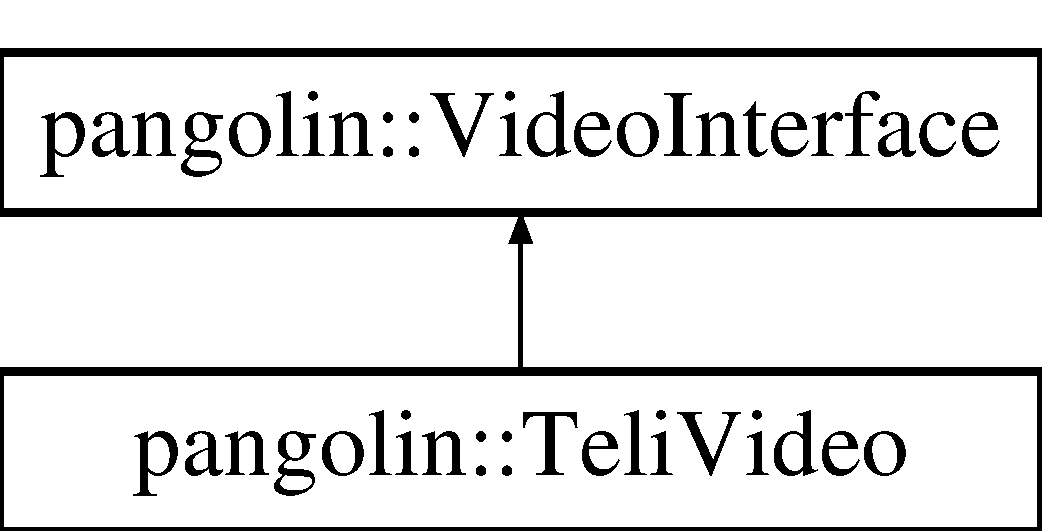
\includegraphics[height=2.000000cm]{classpangolin_1_1_teli_video}
\end{center}
\end{figure}
\subsection*{Public Member Functions}
\begin{DoxyCompactItemize}
\item 
{\bfseries Teli\+Video} (const \hyperlink{structpangolin_1_1_image_roi}{Image\+Roi} \&roi)\hypertarget{classpangolin_1_1_teli_video_a597ca7e6de3d47181e1489709ccdf241}{}\label{classpangolin_1_1_teli_video_a597ca7e6de3d47181e1489709ccdf241}

\item 
void \hyperlink{classpangolin_1_1_teli_video_a9a4993c830eb6e03c45f1959860f0fbf}{Start} ()\hypertarget{classpangolin_1_1_teli_video_a9a4993c830eb6e03c45f1959860f0fbf}{}\label{classpangolin_1_1_teli_video_a9a4993c830eb6e03c45f1959860f0fbf}

\begin{DoxyCompactList}\small\item\em Implement \hyperlink{structpangolin_1_1_video_input_a74a2e3e1b87c7cbf9de9bcb39e1df128}{Video\+Input\+::\+Start()} \end{DoxyCompactList}\item 
void \hyperlink{classpangolin_1_1_teli_video_a16d504baeb4fd27205841e6dc00a53ea}{Stop} ()\hypertarget{classpangolin_1_1_teli_video_a16d504baeb4fd27205841e6dc00a53ea}{}\label{classpangolin_1_1_teli_video_a16d504baeb4fd27205841e6dc00a53ea}

\begin{DoxyCompactList}\small\item\em Implement \hyperlink{structpangolin_1_1_video_input_a8945f80194cc7ec9594db7f27e7d09b8}{Video\+Input\+::\+Stop()} \end{DoxyCompactList}\item 
size\+\_\+t \hyperlink{classpangolin_1_1_teli_video_a016bd1b34e8943313484e28dd82c0ef7}{Size\+Bytes} () const \hypertarget{classpangolin_1_1_teli_video_a016bd1b34e8943313484e28dd82c0ef7}{}\label{classpangolin_1_1_teli_video_a016bd1b34e8943313484e28dd82c0ef7}

\begin{DoxyCompactList}\small\item\em Implement \hyperlink{structpangolin_1_1_video_input_a93cee5c33386973a2a51165e6bdcf40b}{Video\+Input\+::\+Size\+Bytes()} \end{DoxyCompactList}\item 
const std\+::vector$<$ \hyperlink{classpangolin_1_1_stream_info}{Stream\+Info} $>$ \& \hyperlink{classpangolin_1_1_teli_video_a7faa61d4470f1c4565e39e490a7f96b7}{Streams} () const \hypertarget{classpangolin_1_1_teli_video_a7faa61d4470f1c4565e39e490a7f96b7}{}\label{classpangolin_1_1_teli_video_a7faa61d4470f1c4565e39e490a7f96b7}

\begin{DoxyCompactList}\small\item\em Implement \hyperlink{structpangolin_1_1_video_input_a9030d775d699c39ab7b7ba378c007c6a}{Video\+Input\+::\+Streams()} \end{DoxyCompactList}\item 
bool \hyperlink{classpangolin_1_1_teli_video_a29f7574bd0023de05502bb91eb8c16f6}{Grab\+Next} (unsigned char $\ast$image, bool wait=true)\hypertarget{classpangolin_1_1_teli_video_a29f7574bd0023de05502bb91eb8c16f6}{}\label{classpangolin_1_1_teli_video_a29f7574bd0023de05502bb91eb8c16f6}

\begin{DoxyCompactList}\small\item\em Implement \hyperlink{structpangolin_1_1_video_input_ad3d8ff59c1ec4139320097e6e1111f32}{Video\+Input\+::\+Grab\+Next()} \end{DoxyCompactList}\item 
bool \hyperlink{classpangolin_1_1_teli_video_af28ec505e96eb66695b05b1869046e68}{Grab\+Newest} (unsigned char $\ast$image, bool wait=true)\hypertarget{classpangolin_1_1_teli_video_af28ec505e96eb66695b05b1869046e68}{}\label{classpangolin_1_1_teli_video_af28ec505e96eb66695b05b1869046e68}

\begin{DoxyCompactList}\small\item\em Implement \hyperlink{structpangolin_1_1_video_input_a4c8ac38e3c6a3f591663aeebf645e4c6}{Video\+Input\+::\+Grab\+Newest()} \end{DoxyCompactList}\item 
Teli\+::\+C\+A\+M\+\_\+\+H\+A\+N\+D\+LE {\bfseries Get\+Camera\+Handle} ()\hypertarget{classpangolin_1_1_teli_video_a3103d81468614fbf8b3d81a363644f0f}{}\label{classpangolin_1_1_teli_video_a3103d81468614fbf8b3d81a363644f0f}

\item 
Teli\+::\+C\+A\+M\+\_\+\+S\+T\+R\+M\+\_\+\+H\+A\+N\+D\+LE {\bfseries Get\+Camera\+Stream\+Handle} ()\hypertarget{classpangolin_1_1_teli_video_a2b6aa00be8a28a60b959d810bbaaf834}{}\label{classpangolin_1_1_teli_video_a2b6aa00be8a28a60b959d810bbaaf834}

\end{DoxyCompactItemize}
\subsection*{Protected Member Functions}
\begin{DoxyCompactItemize}
\item 
void {\bfseries Initialise} (const \hyperlink{structpangolin_1_1_image_roi}{Image\+Roi} \&roi)\hypertarget{classpangolin_1_1_teli_video_a64a2efd48df09efdac4ca49702a0f628}{}\label{classpangolin_1_1_teli_video_a64a2efd48df09efdac4ca49702a0f628}

\end{DoxyCompactItemize}
\subsection*{Protected Attributes}
\begin{DoxyCompactItemize}
\item 
std\+::vector$<$ \hyperlink{classpangolin_1_1_stream_info}{Stream\+Info} $>$ {\bfseries streams}\hypertarget{classpangolin_1_1_teli_video_a46df18eef216bc5dee27599686b0c753}{}\label{classpangolin_1_1_teli_video_a46df18eef216bc5dee27599686b0c753}

\item 
size\+\_\+t {\bfseries size\+\_\+bytes}\hypertarget{classpangolin_1_1_teli_video_a354424e529443bb44f119ea5becffcfe}{}\label{classpangolin_1_1_teli_video_a354424e529443bb44f119ea5becffcfe}

\item 
Teli\+::\+C\+A\+M\+\_\+\+H\+A\+N\+D\+LE {\bfseries cam}\hypertarget{classpangolin_1_1_teli_video_ad8c5e06a14d24e9dc325e42d5db1de92}{}\label{classpangolin_1_1_teli_video_ad8c5e06a14d24e9dc325e42d5db1de92}

\item 
Teli\+::\+C\+A\+M\+\_\+\+S\+T\+R\+M\+\_\+\+H\+A\+N\+D\+LE {\bfseries strm}\hypertarget{classpangolin_1_1_teli_video_af063cb796a5c5f4eccf81047b46f10ee}{}\label{classpangolin_1_1_teli_video_af063cb796a5c5f4eccf81047b46f10ee}

\item 
H\+A\+N\+D\+LE {\bfseries h\+Strm\+Cmp\+Evt}\hypertarget{classpangolin_1_1_teli_video_ac08bae80c6f8a617d9d0c5717ccb07ba}{}\label{classpangolin_1_1_teli_video_ac08bae80c6f8a617d9d0c5717ccb07ba}

\end{DoxyCompactItemize}


The documentation for this class was generated from the following file\+:\begin{DoxyCompactItemize}
\item 
/home/gapo/meng/deps/pangolin/include/pangolin/video/drivers/teli.\+h\end{DoxyCompactItemize}

\hypertarget{classpangolin_1_1_test_video}{}\section{pangolin\+:\+:Test\+Video Class Reference}
\label{classpangolin_1_1_test_video}\index{pangolin\+::\+Test\+Video@{pangolin\+::\+Test\+Video}}
Inheritance diagram for pangolin\+:\+:Test\+Video\+:\begin{figure}[H]
\begin{center}
\leavevmode
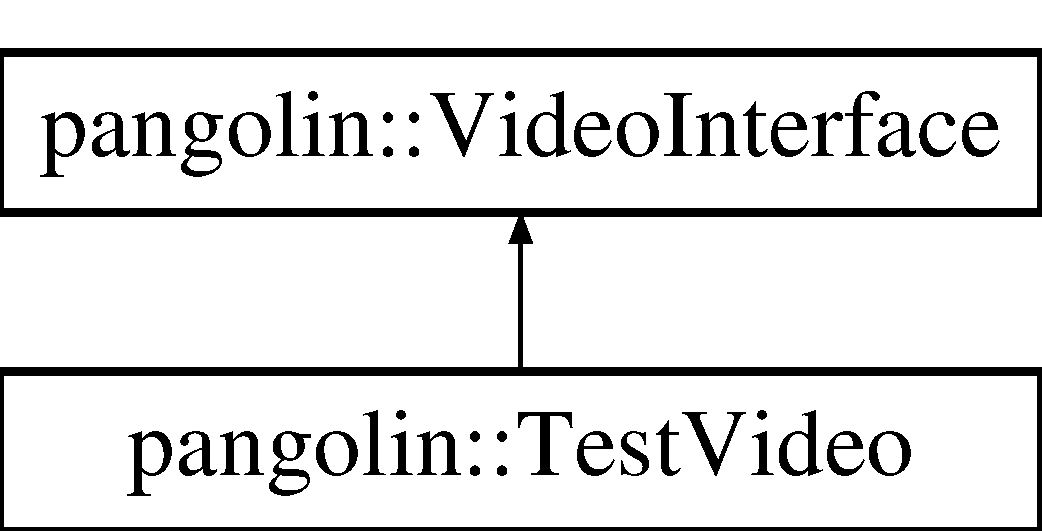
\includegraphics[height=2.000000cm]{classpangolin_1_1_test_video}
\end{center}
\end{figure}
\subsection*{Public Member Functions}
\begin{DoxyCompactItemize}
\item 
{\bfseries Test\+Video} (size\+\_\+t w, size\+\_\+t h, size\+\_\+t n, std\+::string pix\+\_\+fmt)\hypertarget{classpangolin_1_1_test_video_a105e38d101069bd5f517cc621dc26c23}{}\label{classpangolin_1_1_test_video_a105e38d101069bd5f517cc621dc26c23}

\item 
void \hyperlink{classpangolin_1_1_test_video_a2c27959ae2308b533d0eaa4adedfbb51}{Start} ()\hypertarget{classpangolin_1_1_test_video_a2c27959ae2308b533d0eaa4adedfbb51}{}\label{classpangolin_1_1_test_video_a2c27959ae2308b533d0eaa4adedfbb51}

\begin{DoxyCompactList}\small\item\em Implement \hyperlink{structpangolin_1_1_video_input_a74a2e3e1b87c7cbf9de9bcb39e1df128}{Video\+Input\+::\+Start()} \end{DoxyCompactList}\item 
void \hyperlink{classpangolin_1_1_test_video_aa162ae54699f6a5b9b861563ffe1cd64}{Stop} ()\hypertarget{classpangolin_1_1_test_video_aa162ae54699f6a5b9b861563ffe1cd64}{}\label{classpangolin_1_1_test_video_aa162ae54699f6a5b9b861563ffe1cd64}

\begin{DoxyCompactList}\small\item\em Implement \hyperlink{structpangolin_1_1_video_input_a8945f80194cc7ec9594db7f27e7d09b8}{Video\+Input\+::\+Stop()} \end{DoxyCompactList}\item 
size\+\_\+t \hyperlink{classpangolin_1_1_test_video_ab20b4f0d5e1ccdd7a6c40a82a894ed1b}{Size\+Bytes} () const \hypertarget{classpangolin_1_1_test_video_ab20b4f0d5e1ccdd7a6c40a82a894ed1b}{}\label{classpangolin_1_1_test_video_ab20b4f0d5e1ccdd7a6c40a82a894ed1b}

\begin{DoxyCompactList}\small\item\em Implement \hyperlink{structpangolin_1_1_video_input_a93cee5c33386973a2a51165e6bdcf40b}{Video\+Input\+::\+Size\+Bytes()} \end{DoxyCompactList}\item 
const std\+::vector$<$ \hyperlink{classpangolin_1_1_stream_info}{Stream\+Info} $>$ \& \hyperlink{classpangolin_1_1_test_video_ad04e6261b59630b90a2a1011280fb4f1}{Streams} () const \hypertarget{classpangolin_1_1_test_video_ad04e6261b59630b90a2a1011280fb4f1}{}\label{classpangolin_1_1_test_video_ad04e6261b59630b90a2a1011280fb4f1}

\begin{DoxyCompactList}\small\item\em Implement \hyperlink{structpangolin_1_1_video_input_a9030d775d699c39ab7b7ba378c007c6a}{Video\+Input\+::\+Streams()} \end{DoxyCompactList}\item 
bool \hyperlink{classpangolin_1_1_test_video_acc560f46c0a4ed75aa1e99b770eca8d2}{Grab\+Next} (unsigned char $\ast$image, bool wait=true)\hypertarget{classpangolin_1_1_test_video_acc560f46c0a4ed75aa1e99b770eca8d2}{}\label{classpangolin_1_1_test_video_acc560f46c0a4ed75aa1e99b770eca8d2}

\begin{DoxyCompactList}\small\item\em Implement \hyperlink{structpangolin_1_1_video_input_ad3d8ff59c1ec4139320097e6e1111f32}{Video\+Input\+::\+Grab\+Next()} \end{DoxyCompactList}\item 
bool \hyperlink{classpangolin_1_1_test_video_aa85934d2fabe70de53c27bf55443bb4f}{Grab\+Newest} (unsigned char $\ast$image, bool wait=true)\hypertarget{classpangolin_1_1_test_video_aa85934d2fabe70de53c27bf55443bb4f}{}\label{classpangolin_1_1_test_video_aa85934d2fabe70de53c27bf55443bb4f}

\begin{DoxyCompactList}\small\item\em Implement \hyperlink{structpangolin_1_1_video_input_a4c8ac38e3c6a3f591663aeebf645e4c6}{Video\+Input\+::\+Grab\+Newest()} \end{DoxyCompactList}\end{DoxyCompactItemize}
\subsection*{Protected Attributes}
\begin{DoxyCompactItemize}
\item 
std\+::vector$<$ \hyperlink{classpangolin_1_1_stream_info}{Stream\+Info} $>$ {\bfseries streams}\hypertarget{classpangolin_1_1_test_video_abde8d7a1dbdcc210d7bd3925c3ed3e38}{}\label{classpangolin_1_1_test_video_abde8d7a1dbdcc210d7bd3925c3ed3e38}

\item 
size\+\_\+t {\bfseries size\+\_\+bytes}\hypertarget{classpangolin_1_1_test_video_a66692e2656abd48a7acea11a893453a6}{}\label{classpangolin_1_1_test_video_a66692e2656abd48a7acea11a893453a6}

\end{DoxyCompactItemize}


The documentation for this class was generated from the following file\+:\begin{DoxyCompactItemize}
\item 
/home/gapo/meng/deps/pangolin/include/pangolin/video/drivers/test.\+h\end{DoxyCompactItemize}

\hypertarget{structpangolin_1_1_text_input}{}\section{pangolin\+:\+:Text\+Input Struct Reference}
\label{structpangolin_1_1_text_input}\index{pangolin\+::\+Text\+Input@{pangolin\+::\+Text\+Input}}
Inheritance diagram for pangolin\+:\+:Text\+Input\+:\begin{figure}[H]
\begin{center}
\leavevmode
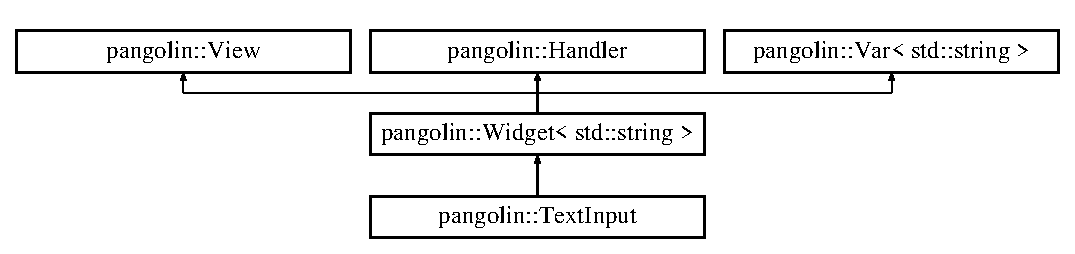
\includegraphics[height=2.962963cm]{structpangolin_1_1_text_input}
\end{center}
\end{figure}
\subsection*{Public Member Functions}
\begin{DoxyCompactItemize}
\item 
{\bfseries Text\+Input} (std\+::string title, \hyperlink{classpangolin_1_1_var_value_generic}{Var\+Value\+Generic} \&tv)\hypertarget{structpangolin_1_1_text_input_a1e3121ac096852641d4c284250751717}{}\label{structpangolin_1_1_text_input_a1e3121ac096852641d4c284250751717}

\item 
void {\bfseries Mouse} (\hyperlink{structpangolin_1_1_view}{View} \&, Mouse\+Button button, int x, int y, bool pressed, int mouse\+\_\+state)\hypertarget{structpangolin_1_1_text_input_a27d416092e825c4c21322188f643c9cc}{}\label{structpangolin_1_1_text_input_a27d416092e825c4c21322188f643c9cc}

\item 
void {\bfseries Mouse\+Motion} (\hyperlink{structpangolin_1_1_view}{View} \&, int x, int y, int mouse\+\_\+state)\hypertarget{structpangolin_1_1_text_input_a2c6deff3d77227cf4353a9d27553a54e}{}\label{structpangolin_1_1_text_input_a2c6deff3d77227cf4353a9d27553a54e}

\item 
void {\bfseries Keyboard} (\hyperlink{structpangolin_1_1_view}{View} \&, unsigned char key, int x, int y, bool pressed)\hypertarget{structpangolin_1_1_text_input_a069e3ebdc0567c22152d47d96d29c5df}{}\label{structpangolin_1_1_text_input_a069e3ebdc0567c22152d47d96d29c5df}

\item 
void \hyperlink{structpangolin_1_1_text_input_a76fba1c1f6ececafa48b393b5a823944}{Render} ()
\begin{DoxyCompactList}\small\item\em Perform any automatic rendering for this \hyperlink{structpangolin_1_1_view}{View}. \end{DoxyCompactList}\item 
void \hyperlink{structpangolin_1_1_text_input_a2d749a3cd765aebceb05310152559897}{Resize\+Children} ()\hypertarget{structpangolin_1_1_text_input_a2d749a3cd765aebceb05310152559897}{}\label{structpangolin_1_1_text_input_a2d749a3cd765aebceb05310152559897}

\begin{DoxyCompactList}\small\item\em Instruct all children to resize. \end{DoxyCompactList}\end{DoxyCompactItemize}
\subsection*{Public Attributes}
\begin{DoxyCompactItemize}
\item 
std\+::string {\bfseries edit}\hypertarget{structpangolin_1_1_text_input_a7c43bd80c89d0b3819094c9da5c07ed7}{}\label{structpangolin_1_1_text_input_a7c43bd80c89d0b3819094c9da5c07ed7}

\item 
\hyperlink{classpangolin_1_1_gl_text}{Gl\+Text} {\bfseries gledit}\hypertarget{structpangolin_1_1_text_input_af5289e2ead9b59a5d3498478c6c33670}{}\label{structpangolin_1_1_text_input_af5289e2ead9b59a5d3498478c6c33670}

\item 
\hyperlink{classpangolin_1_1_gl_text}{Gl\+Text} {\bfseries gltext}\hypertarget{structpangolin_1_1_text_input_aa6e230140d88326e64b318870a9b35ec}{}\label{structpangolin_1_1_text_input_aa6e230140d88326e64b318870a9b35ec}

\item 
G\+Lfloat {\bfseries raster} \mbox{[}2\mbox{]}\hypertarget{structpangolin_1_1_text_input_a56759b64810ab00dea80bca2da47accd}{}\label{structpangolin_1_1_text_input_a56759b64810ab00dea80bca2da47accd}

\item 
bool {\bfseries do\+\_\+edit}\hypertarget{structpangolin_1_1_text_input_aefd15e802c99da15131edc87a4748d8c}{}\label{structpangolin_1_1_text_input_aefd15e802c99da15131edc87a4748d8c}

\item 
int {\bfseries sel} \mbox{[}2\mbox{]}\hypertarget{structpangolin_1_1_text_input_a687bcacda8b3bf0432202145bdd0c262}{}\label{structpangolin_1_1_text_input_a687bcacda8b3bf0432202145bdd0c262}

\end{DoxyCompactItemize}
\subsection*{Additional Inherited Members}


\subsection{Member Function Documentation}
\index{pangolin\+::\+Text\+Input@{pangolin\+::\+Text\+Input}!Render@{Render}}
\index{Render@{Render}!pangolin\+::\+Text\+Input@{pangolin\+::\+Text\+Input}}
\subsubsection[{\texorpdfstring{Render()}{Render()}}]{\setlength{\rightskip}{0pt plus 5cm}void pangolin\+::\+Text\+Input\+::\+Render (
\begin{DoxyParamCaption}
{}
\end{DoxyParamCaption}
)\hspace{0.3cm}{\ttfamily [virtual]}}\hypertarget{structpangolin_1_1_text_input_a76fba1c1f6ececafa48b393b5a823944}{}\label{structpangolin_1_1_text_input_a76fba1c1f6ececafa48b393b5a823944}


Perform any automatic rendering for this \hyperlink{structpangolin_1_1_view}{View}. 

Default implementation simply instructs children to render themselves. 

Reimplemented from \hyperlink{structpangolin_1_1_view_a15bf43d7ebc4ebe4e02cba572f0d49ba}{pangolin\+::\+View}.



The documentation for this struct was generated from the following file\+:\begin{DoxyCompactItemize}
\item 
/home/gapo/meng/deps/pangolin/include/pangolin/display/widgets/widgets.\+h\end{DoxyCompactItemize}

\hypertarget{classpangolin_1_1_texture_cache}{}\section{pangolin\+:\+:Texture\+Cache Class Reference}
\label{classpangolin_1_1_texture_cache}\index{pangolin\+::\+Texture\+Cache@{pangolin\+::\+Texture\+Cache}}
\subsection*{Public Member Functions}
\begin{DoxyCompactItemize}
\item 
\hyperlink{classpangolin_1_1_gl_texture}{Gl\+Texture} \& {\bfseries Gl\+Tex} (int w, int h, G\+Lint internal\+\_\+format, G\+Lint glformat, G\+Lenum gltype)\hypertarget{classpangolin_1_1_texture_cache_ac0ac9e8698d23b54f7b28a83af2938b8}{}\label{classpangolin_1_1_texture_cache_ac0ac9e8698d23b54f7b28a83af2938b8}

\item 
{\footnotesize template$<$typename T $>$ }\\\hyperlink{classpangolin_1_1_gl_texture}{Gl\+Texture} \& {\bfseries Gl\+Tex} (int w, int h)\hypertarget{classpangolin_1_1_texture_cache_a070a94044a40d7156ec8d6ea578bb0c1}{}\label{classpangolin_1_1_texture_cache_a070a94044a40d7156ec8d6ea578bb0c1}

\end{DoxyCompactItemize}
\subsection*{Static Public Member Functions}
\begin{DoxyCompactItemize}
\item 
static \hyperlink{classpangolin_1_1_texture_cache}{Texture\+Cache} \& {\bfseries I} ()\hypertarget{classpangolin_1_1_texture_cache_af76862570e07ab2ce8f140b15f7f5a0b}{}\label{classpangolin_1_1_texture_cache_af76862570e07ab2ce8f140b15f7f5a0b}

\end{DoxyCompactItemize}
\subsection*{Protected Attributes}
\begin{DoxyCompactItemize}
\item 
bool {\bfseries default\+\_\+sampling\+\_\+linear}\hypertarget{classpangolin_1_1_texture_cache_afe66eb49ba5077914885c329f686b64b}{}\label{classpangolin_1_1_texture_cache_afe66eb49ba5077914885c329f686b64b}

\item 
std\+::map$<$ long, boostd\+::shared\+\_\+ptr$<$ \hyperlink{classpangolin_1_1_gl_texture}{Gl\+Texture} $>$ $>$ {\bfseries texture\+\_\+map}\hypertarget{classpangolin_1_1_texture_cache_a27d3d17fd66266a057bc2dffe91a4c3f}{}\label{classpangolin_1_1_texture_cache_a27d3d17fd66266a057bc2dffe91a4c3f}

\end{DoxyCompactItemize}


The documentation for this class was generated from the following file\+:\begin{DoxyCompactItemize}
\item 
/home/gapo/meng/deps/pangolin/include/pangolin/gl/gltexturecache.\+h\end{DoxyCompactItemize}

\hypertarget{classpangolin_1_1threadedfilebuf}{}\section{pangolin\+:\+:threadedfilebuf Class Reference}
\label{classpangolin_1_1threadedfilebuf}\index{pangolin\+::threadedfilebuf@{pangolin\+::threadedfilebuf}}
Inheritance diagram for pangolin\+:\+:threadedfilebuf\+:\begin{figure}[H]
\begin{center}
\leavevmode
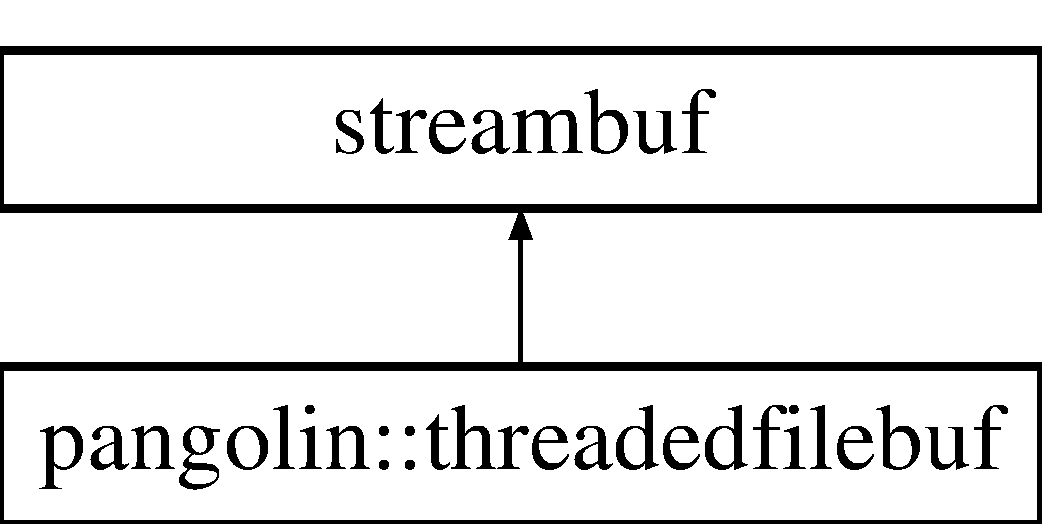
\includegraphics[height=2.000000cm]{classpangolin_1_1threadedfilebuf}
\end{center}
\end{figure}
\subsection*{Public Member Functions}
\begin{DoxyCompactItemize}
\item 
{\bfseries threadedfilebuf} (const std\+::string \&filename, unsigned int buffer\+\_\+size\+\_\+bytes)\hypertarget{classpangolin_1_1threadedfilebuf_a1f8f48af4418b08e5858476db6a0bf7d}{}\label{classpangolin_1_1threadedfilebuf_a1f8f48af4418b08e5858476db6a0bf7d}

\item 
void {\bfseries open} (const std\+::string \&filename, unsigned int buffer\+\_\+size\+\_\+bytes)\hypertarget{classpangolin_1_1threadedfilebuf_ac2bbd1798e737480bbbcddb70e8bf286}{}\label{classpangolin_1_1threadedfilebuf_ac2bbd1798e737480bbbcddb70e8bf286}

\item 
void {\bfseries close} ()\hypertarget{classpangolin_1_1threadedfilebuf_a26caf0a8836f0a095f0c34b1f8e16eb5}{}\label{classpangolin_1_1threadedfilebuf_a26caf0a8836f0a095f0c34b1f8e16eb5}

\item 
void {\bfseries operator()} ()\hypertarget{classpangolin_1_1threadedfilebuf_a0eda1c760b1fbca3866af2b9db630c61}{}\label{classpangolin_1_1threadedfilebuf_a0eda1c760b1fbca3866af2b9db630c61}

\end{DoxyCompactItemize}
\subsection*{Protected Member Functions}
\begin{DoxyCompactItemize}
\item 
std\+::streamsize \hyperlink{classpangolin_1_1threadedfilebuf_afcc794e847ef4313a4655d3352013bed}{xsputn} (const char $\ast$s, std\+::streamsize n)\hypertarget{classpangolin_1_1threadedfilebuf_afcc794e847ef4313a4655d3352013bed}{}\label{classpangolin_1_1threadedfilebuf_afcc794e847ef4313a4655d3352013bed}

\begin{DoxyCompactList}\small\item\em Override streambuf\+::xsputn for asynchronous write. \end{DoxyCompactList}\item 
int \hyperlink{classpangolin_1_1threadedfilebuf_ace93103b8c732bdf7ad2563eea9e3cde}{overflow} (int c)\hypertarget{classpangolin_1_1threadedfilebuf_ace93103b8c732bdf7ad2563eea9e3cde}{}\label{classpangolin_1_1threadedfilebuf_ace93103b8c732bdf7ad2563eea9e3cde}

\begin{DoxyCompactList}\small\item\em Override streambuf\+::overflow for asynchronous write. \end{DoxyCompactList}\end{DoxyCompactItemize}
\subsection*{Protected Attributes}
\begin{DoxyCompactItemize}
\item 
std\+::filebuf {\bfseries file}\hypertarget{classpangolin_1_1threadedfilebuf_a373fcf09776cc1868c4ff08c333c7c3c}{}\label{classpangolin_1_1threadedfilebuf_a373fcf09776cc1868c4ff08c333c7c3c}

\item 
char $\ast$ {\bfseries mem\+\_\+buffer}\hypertarget{classpangolin_1_1threadedfilebuf_aac3ce17357da2f6e81ebc77c5e998c71}{}\label{classpangolin_1_1threadedfilebuf_aac3ce17357da2f6e81ebc77c5e998c71}

\item 
std\+::streamsize {\bfseries mem\+\_\+size}\hypertarget{classpangolin_1_1threadedfilebuf_aba55337f4f0132177ad5c27ae968377b}{}\label{classpangolin_1_1threadedfilebuf_aba55337f4f0132177ad5c27ae968377b}

\item 
std\+::streamsize {\bfseries mem\+\_\+max\+\_\+size}\hypertarget{classpangolin_1_1threadedfilebuf_a4804e187ba87430eb131ff46f2d88fe6}{}\label{classpangolin_1_1threadedfilebuf_a4804e187ba87430eb131ff46f2d88fe6}

\item 
std\+::streamsize {\bfseries mem\+\_\+start}\hypertarget{classpangolin_1_1threadedfilebuf_aa17442e2f4d97662f0c88f8b17eac1fa}{}\label{classpangolin_1_1threadedfilebuf_aa17442e2f4d97662f0c88f8b17eac1fa}

\item 
std\+::streamsize {\bfseries mem\+\_\+end}\hypertarget{classpangolin_1_1threadedfilebuf_a7a0424da5568a7095dd194e26ecaf071}{}\label{classpangolin_1_1threadedfilebuf_a7a0424da5568a7095dd194e26ecaf071}

\item 
boostd\+::mutex {\bfseries update\+\_\+mutex}\hypertarget{classpangolin_1_1threadedfilebuf_ad333f1455ad1d081ba1a0d55a02c9945}{}\label{classpangolin_1_1threadedfilebuf_ad333f1455ad1d081ba1a0d55a02c9945}

\item 
boostd\+::condition\+\_\+variable {\bfseries cond\+\_\+queued}\hypertarget{classpangolin_1_1threadedfilebuf_aae1332b77e84426cd16ec85e43c611f6}{}\label{classpangolin_1_1threadedfilebuf_aae1332b77e84426cd16ec85e43c611f6}

\item 
boostd\+::condition\+\_\+variable {\bfseries cond\+\_\+dequeued}\hypertarget{classpangolin_1_1threadedfilebuf_a4cd70c2f2d254f271e42c19d852266b5}{}\label{classpangolin_1_1threadedfilebuf_a4cd70c2f2d254f271e42c19d852266b5}

\item 
boostd\+::thread {\bfseries write\+\_\+thread}\hypertarget{classpangolin_1_1threadedfilebuf_a59913f59bafc9ed2aaa27f02ec23fe73}{}\label{classpangolin_1_1threadedfilebuf_a59913f59bafc9ed2aaa27f02ec23fe73}

\item 
bool {\bfseries should\+\_\+run}\hypertarget{classpangolin_1_1threadedfilebuf_aa9f98f7b857d6ef1b5cdd0fe9061eb95}{}\label{classpangolin_1_1threadedfilebuf_aa9f98f7b857d6ef1b5cdd0fe9061eb95}

\end{DoxyCompactItemize}


The documentation for this class was generated from the following file\+:\begin{DoxyCompactItemize}
\item 
/home/gapo/meng/deps/pangolin/include/pangolin/utils/threadedfilebuf.\+h\end{DoxyCompactItemize}

\hypertarget{structpangolin_1_1_plotter_1_1_tick}{}\section{pangolin\+:\+:Plotter\+:\+:Tick Struct Reference}
\label{structpangolin_1_1_plotter_1_1_tick}\index{pangolin\+::\+Plotter\+::\+Tick@{pangolin\+::\+Plotter\+::\+Tick}}
\subsection*{Public Attributes}
\begin{DoxyCompactItemize}
\item 
float {\bfseries val}\hypertarget{structpangolin_1_1_plotter_1_1_tick_a0d35931e9b62a62e188f70e373d11fc5}{}\label{structpangolin_1_1_plotter_1_1_tick_a0d35931e9b62a62e188f70e373d11fc5}

\item 
float {\bfseries factor}\hypertarget{structpangolin_1_1_plotter_1_1_tick_a88175ec4eee1e1e5cd427e2c092c72a1}{}\label{structpangolin_1_1_plotter_1_1_tick_a88175ec4eee1e1e5cd427e2c092c72a1}

\item 
std\+::string {\bfseries symbol}\hypertarget{structpangolin_1_1_plotter_1_1_tick_a5cdfdd47c7fcda2aa6036011b6d97446}{}\label{structpangolin_1_1_plotter_1_1_tick_a5cdfdd47c7fcda2aa6036011b6d97446}

\end{DoxyCompactItemize}


The documentation for this struct was generated from the following file\+:\begin{DoxyCompactItemize}
\item 
/home/gapo/meng/deps/pangolin/include/pangolin/plot/plotter.\+h\end{DoxyCompactItemize}

\hypertarget{structpangolin_1_1_timer}{}\section{pangolin\+:\+:Timer Struct Reference}
\label{structpangolin_1_1_timer}\index{pangolin\+::\+Timer@{pangolin\+::\+Timer}}
\subsection*{Public Member Functions}
\begin{DoxyCompactItemize}
\item 
void {\bfseries Reset} ()\hypertarget{structpangolin_1_1_timer_aaf0b01ec01f44c5da0241625beb71123}{}\label{structpangolin_1_1_timer_aaf0b01ec01f44c5da0241625beb71123}

\item 
double {\bfseries Elapsed\+\_\+s} ()\hypertarget{structpangolin_1_1_timer_a6eb771a3f219d6ec5239a9bee8a41bca}{}\label{structpangolin_1_1_timer_a6eb771a3f219d6ec5239a9bee8a41bca}

\end{DoxyCompactItemize}
\subsection*{Public Attributes}
\begin{DoxyCompactItemize}
\item 
basetime {\bfseries start}\hypertarget{structpangolin_1_1_timer_aa85a5e1e1804896d257c9dc0f97bdd15}{}\label{structpangolin_1_1_timer_aa85a5e1e1804896d257c9dc0f97bdd15}

\end{DoxyCompactItemize}


The documentation for this struct was generated from the following file\+:\begin{DoxyCompactItemize}
\item 
/home/gapo/meng/deps/pangolin/include/pangolin/utils/timer.\+h\end{DoxyCompactItemize}

\hypertarget{structpangolin_1_1_toggle_var_functor}{}\section{pangolin\+:\+:Toggle\+Var\+Functor Struct Reference}
\label{structpangolin_1_1_toggle_var_functor}\index{pangolin\+::\+Toggle\+Var\+Functor@{pangolin\+::\+Toggle\+Var\+Functor}}
\subsection*{Public Member Functions}
\begin{DoxyCompactItemize}
\item 
{\bfseries Toggle\+Var\+Functor} (const std\+::string \&name)\hypertarget{structpangolin_1_1_toggle_var_functor_a75f9e14ad65576a86f4dd715b2250cbf}{}\label{structpangolin_1_1_toggle_var_functor_a75f9e14ad65576a86f4dd715b2250cbf}

\item 
void {\bfseries operator()} ()\hypertarget{structpangolin_1_1_toggle_var_functor_acaada2ab666dd4f8657591c7fff89e1b}{}\label{structpangolin_1_1_toggle_var_functor_acaada2ab666dd4f8657591c7fff89e1b}

\end{DoxyCompactItemize}
\subsection*{Public Attributes}
\begin{DoxyCompactItemize}
\item 
std\+::string {\bfseries var\+Name}\hypertarget{structpangolin_1_1_toggle_var_functor_aa42d93a5b72621880dc2c3ea3f88fa50}{}\label{structpangolin_1_1_toggle_var_functor_aa42d93a5b72621880dc2c3ea3f88fa50}

\end{DoxyCompactItemize}


The documentation for this struct was generated from the following file\+:\begin{DoxyCompactItemize}
\item 
/home/gapo/meng/deps/pangolin/include/pangolin/var/varextra.\+h\end{DoxyCompactItemize}

\hypertarget{structpangolin_1_1_toggle_view_functor}{}\section{pangolin\+:\+:Toggle\+View\+Functor Struct Reference}
\label{structpangolin_1_1_toggle_view_functor}\index{pangolin\+::\+Toggle\+View\+Functor@{pangolin\+::\+Toggle\+View\+Functor}}


Convenience functor for toggling \hyperlink{structpangolin_1_1_view}{pangolin\+::\+View}.  




{\ttfamily \#include $<$display.\+h$>$}

\subsection*{Public Member Functions}
\begin{DoxyCompactItemize}
\item 
{\bfseries Toggle\+View\+Functor} (\hyperlink{structpangolin_1_1_view}{View} \&view)\hypertarget{structpangolin_1_1_toggle_view_functor_a61d137ec3da01e7276cd016d6bdf8c89}{}\label{structpangolin_1_1_toggle_view_functor_a61d137ec3da01e7276cd016d6bdf8c89}

\item 
{\bfseries Toggle\+View\+Functor} (const std\+::string \&name)\hypertarget{structpangolin_1_1_toggle_view_functor_a4cb0e9c355570b331acd7b050e0f1588}{}\label{structpangolin_1_1_toggle_view_functor_a4cb0e9c355570b331acd7b050e0f1588}

\item 
void {\bfseries operator()} ()\hypertarget{structpangolin_1_1_toggle_view_functor_a991cfb0162fb4b7bee1c60257ca9e051}{}\label{structpangolin_1_1_toggle_view_functor_a991cfb0162fb4b7bee1c60257ca9e051}

\end{DoxyCompactItemize}
\subsection*{Public Attributes}
\begin{DoxyCompactItemize}
\item 
\hyperlink{structpangolin_1_1_view}{View} \& {\bfseries view}\hypertarget{structpangolin_1_1_toggle_view_functor_a0b2f5e0420cebb0820d0c07d979d9b99}{}\label{structpangolin_1_1_toggle_view_functor_a0b2f5e0420cebb0820d0c07d979d9b99}

\end{DoxyCompactItemize}


\subsection{Detailed Description}
Convenience functor for toggling \hyperlink{structpangolin_1_1_view}{pangolin\+::\+View}. 

Use with Register\+Key\+Press\+Callback for example 

The documentation for this struct was generated from the following file\+:\begin{DoxyCompactItemize}
\item 
/home/gapo/meng/deps/pangolin/include/pangolin/display/\hyperlink{display_8h}{display.\+h}\end{DoxyCompactItemize}

\hypertarget{structpangolin_1_1_typed_image}{}\section{pangolin\+:\+:Typed\+Image Struct Reference}
\label{structpangolin_1_1_typed_image}\index{pangolin\+::\+Typed\+Image@{pangolin\+::\+Typed\+Image}}
Inheritance diagram for pangolin\+:\+:Typed\+Image\+:\begin{figure}[H]
\begin{center}
\leavevmode
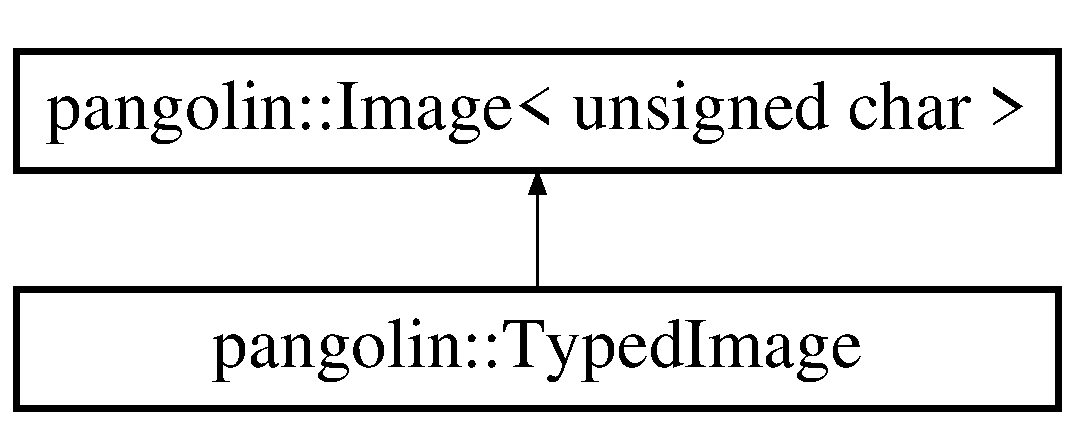
\includegraphics[height=2.000000cm]{structpangolin_1_1_typed_image}
\end{center}
\end{figure}
\subsection*{Public Member Functions}
\begin{DoxyCompactItemize}
\item 
{\bfseries Typed\+Image} (size\+\_\+t w, size\+\_\+t h, size\+\_\+t pitch, unsigned char $\ast$ptr, const \hyperlink{structpangolin_1_1_video_pixel_format}{Video\+Pixel\+Format} \&fmt)\hypertarget{structpangolin_1_1_typed_image_ade52b7d81698f1f3e79d07162c6210af}{}\label{structpangolin_1_1_typed_image_ade52b7d81698f1f3e79d07162c6210af}

\item 
void {\bfseries Alloc} (size\+\_\+t w, size\+\_\+t h, const \hyperlink{structpangolin_1_1_video_pixel_format}{Video\+Pixel\+Format} \&fmt)\hypertarget{structpangolin_1_1_typed_image_a7d09a86f50f02e499e906379f1953ae3}{}\label{structpangolin_1_1_typed_image_a7d09a86f50f02e499e906379f1953ae3}

\item 
void {\bfseries Alloc} (size\+\_\+t w, size\+\_\+t h, const \hyperlink{structpangolin_1_1_video_pixel_format}{Video\+Pixel\+Format} \&fmt, size\+\_\+t pitch)\hypertarget{structpangolin_1_1_typed_image_a8d1456f71e60966f812e15cfde88ff83}{}\label{structpangolin_1_1_typed_image_a8d1456f71e60966f812e15cfde88ff83}

\end{DoxyCompactItemize}
\subsection*{Public Attributes}
\begin{DoxyCompactItemize}
\item 
\hyperlink{structpangolin_1_1_video_pixel_format}{Video\+Pixel\+Format} {\bfseries fmt}\hypertarget{structpangolin_1_1_typed_image_aced9e14a5a9f1a04b038b22458413104}{}\label{structpangolin_1_1_typed_image_aced9e14a5a9f1a04b038b22458413104}

\end{DoxyCompactItemize}


The documentation for this struct was generated from the following file\+:\begin{DoxyCompactItemize}
\item 
/home/gapo/meng/deps/pangolin/include/pangolin/image/image\+\_\+io.\+h\end{DoxyCompactItemize}

\hypertarget{classpangolin_1_1_unpack_video}{}\section{pangolin\+:\+:Unpack\+Video Class Reference}
\label{classpangolin_1_1_unpack_video}\index{pangolin\+::\+Unpack\+Video@{pangolin\+::\+Unpack\+Video}}
Inheritance diagram for pangolin\+:\+:Unpack\+Video\+:\begin{figure}[H]
\begin{center}
\leavevmode
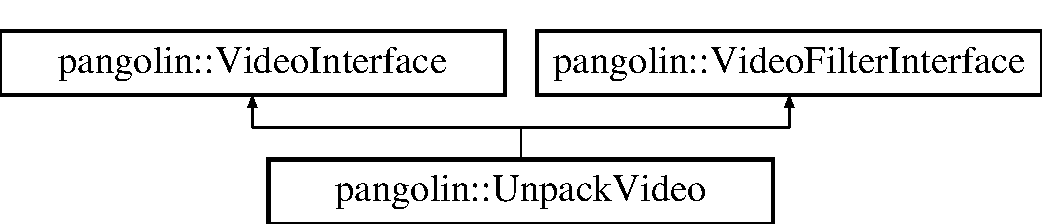
\includegraphics[height=2.000000cm]{classpangolin_1_1_unpack_video}
\end{center}
\end{figure}
\subsection*{Public Member Functions}
\begin{DoxyCompactItemize}
\item 
{\bfseries Unpack\+Video} (\hyperlink{structpangolin_1_1_video_interface}{Video\+Interface} $\ast$videoin, \hyperlink{structpangolin_1_1_video_pixel_format}{Video\+Pixel\+Format} new\+\_\+fmt)\hypertarget{classpangolin_1_1_unpack_video_aa0b5efefb32da50519dd7a0f4689e050}{}\label{classpangolin_1_1_unpack_video_aa0b5efefb32da50519dd7a0f4689e050}

\item 
void \hyperlink{classpangolin_1_1_unpack_video_a41395b8f02a046977e0befff46e41245}{Start} ()\hypertarget{classpangolin_1_1_unpack_video_a41395b8f02a046977e0befff46e41245}{}\label{classpangolin_1_1_unpack_video_a41395b8f02a046977e0befff46e41245}

\begin{DoxyCompactList}\small\item\em Implement \hyperlink{structpangolin_1_1_video_input_a74a2e3e1b87c7cbf9de9bcb39e1df128}{Video\+Input\+::\+Start()} \end{DoxyCompactList}\item 
void \hyperlink{classpangolin_1_1_unpack_video_afd5cf4e9c9f3f712b401f2ab3235f629}{Stop} ()\hypertarget{classpangolin_1_1_unpack_video_afd5cf4e9c9f3f712b401f2ab3235f629}{}\label{classpangolin_1_1_unpack_video_afd5cf4e9c9f3f712b401f2ab3235f629}

\begin{DoxyCompactList}\small\item\em Implement \hyperlink{structpangolin_1_1_video_input_a8945f80194cc7ec9594db7f27e7d09b8}{Video\+Input\+::\+Stop()} \end{DoxyCompactList}\item 
size\+\_\+t \hyperlink{classpangolin_1_1_unpack_video_a298183c1e56972585a340c4580f6a350}{Size\+Bytes} () const \hypertarget{classpangolin_1_1_unpack_video_a298183c1e56972585a340c4580f6a350}{}\label{classpangolin_1_1_unpack_video_a298183c1e56972585a340c4580f6a350}

\begin{DoxyCompactList}\small\item\em Implement \hyperlink{structpangolin_1_1_video_input_a93cee5c33386973a2a51165e6bdcf40b}{Video\+Input\+::\+Size\+Bytes()} \end{DoxyCompactList}\item 
const std\+::vector$<$ \hyperlink{classpangolin_1_1_stream_info}{Stream\+Info} $>$ \& \hyperlink{classpangolin_1_1_unpack_video_a84d5b3d20b1bf0b52d132bc8f4c204ad}{Streams} () const \hypertarget{classpangolin_1_1_unpack_video_a84d5b3d20b1bf0b52d132bc8f4c204ad}{}\label{classpangolin_1_1_unpack_video_a84d5b3d20b1bf0b52d132bc8f4c204ad}

\begin{DoxyCompactList}\small\item\em Implement \hyperlink{structpangolin_1_1_video_input_a9030d775d699c39ab7b7ba378c007c6a}{Video\+Input\+::\+Streams()} \end{DoxyCompactList}\item 
bool \hyperlink{classpangolin_1_1_unpack_video_a51d2246c54897aebb11c579d28eb0cbf}{Grab\+Next} (unsigned char $\ast$image, bool wait=true)\hypertarget{classpangolin_1_1_unpack_video_a51d2246c54897aebb11c579d28eb0cbf}{}\label{classpangolin_1_1_unpack_video_a51d2246c54897aebb11c579d28eb0cbf}

\begin{DoxyCompactList}\small\item\em Implement \hyperlink{structpangolin_1_1_video_input_ad3d8ff59c1ec4139320097e6e1111f32}{Video\+Input\+::\+Grab\+Next()} \end{DoxyCompactList}\item 
bool \hyperlink{classpangolin_1_1_unpack_video_aa93db4c7b979a6bf9bf8e58251244c23}{Grab\+Newest} (unsigned char $\ast$image, bool wait=true)\hypertarget{classpangolin_1_1_unpack_video_aa93db4c7b979a6bf9bf8e58251244c23}{}\label{classpangolin_1_1_unpack_video_aa93db4c7b979a6bf9bf8e58251244c23}

\begin{DoxyCompactList}\small\item\em Implement \hyperlink{structpangolin_1_1_video_input_a4c8ac38e3c6a3f591663aeebf645e4c6}{Video\+Input\+::\+Grab\+Newest()} \end{DoxyCompactList}\item 
std\+::vector$<$ \hyperlink{structpangolin_1_1_video_interface}{Video\+Interface} $\ast$ $>$ \& {\bfseries Input\+Streams} ()\hypertarget{classpangolin_1_1_unpack_video_a523f0d781cb3340bf9f1ab0b385c87c2}{}\label{classpangolin_1_1_unpack_video_a523f0d781cb3340bf9f1ab0b385c87c2}

\end{DoxyCompactItemize}
\subsection*{Protected Attributes}
\begin{DoxyCompactItemize}
\item 
std\+::vector$<$ \hyperlink{structpangolin_1_1_video_interface}{Video\+Interface} $\ast$ $>$ {\bfseries videoin}\hypertarget{classpangolin_1_1_unpack_video_aa37278ebd42ef391ed12859cc3b934a6}{}\label{classpangolin_1_1_unpack_video_aa37278ebd42ef391ed12859cc3b934a6}

\item 
std\+::vector$<$ \hyperlink{classpangolin_1_1_stream_info}{Stream\+Info} $>$ {\bfseries streams}\hypertarget{classpangolin_1_1_unpack_video_a0f78b80d684d95ef0198ba8217a17f6d}{}\label{classpangolin_1_1_unpack_video_a0f78b80d684d95ef0198ba8217a17f6d}

\item 
size\+\_\+t {\bfseries size\+\_\+bytes}\hypertarget{classpangolin_1_1_unpack_video_a07c5cc6343560bac604c224ebf21241f}{}\label{classpangolin_1_1_unpack_video_a07c5cc6343560bac604c224ebf21241f}

\item 
unsigned char $\ast$ {\bfseries buffer}\hypertarget{classpangolin_1_1_unpack_video_a8c5ffa9fa5d6d57acba501224d48a832}{}\label{classpangolin_1_1_unpack_video_a8c5ffa9fa5d6d57acba501224d48a832}

\end{DoxyCompactItemize}


The documentation for this class was generated from the following file\+:\begin{DoxyCompactItemize}
\item 
/home/gapo/meng/deps/pangolin/include/pangolin/video/drivers/unpack.\+h\end{DoxyCompactItemize}

\hypertarget{classpangolin_1_1_uri}{}\section{pangolin\+:\+:Uri Class Reference}
\label{classpangolin_1_1_uri}\index{pangolin\+::\+Uri@{pangolin\+::\+Uri}}
Inheritance diagram for pangolin\+:\+:Uri\+:\begin{figure}[H]
\begin{center}
\leavevmode
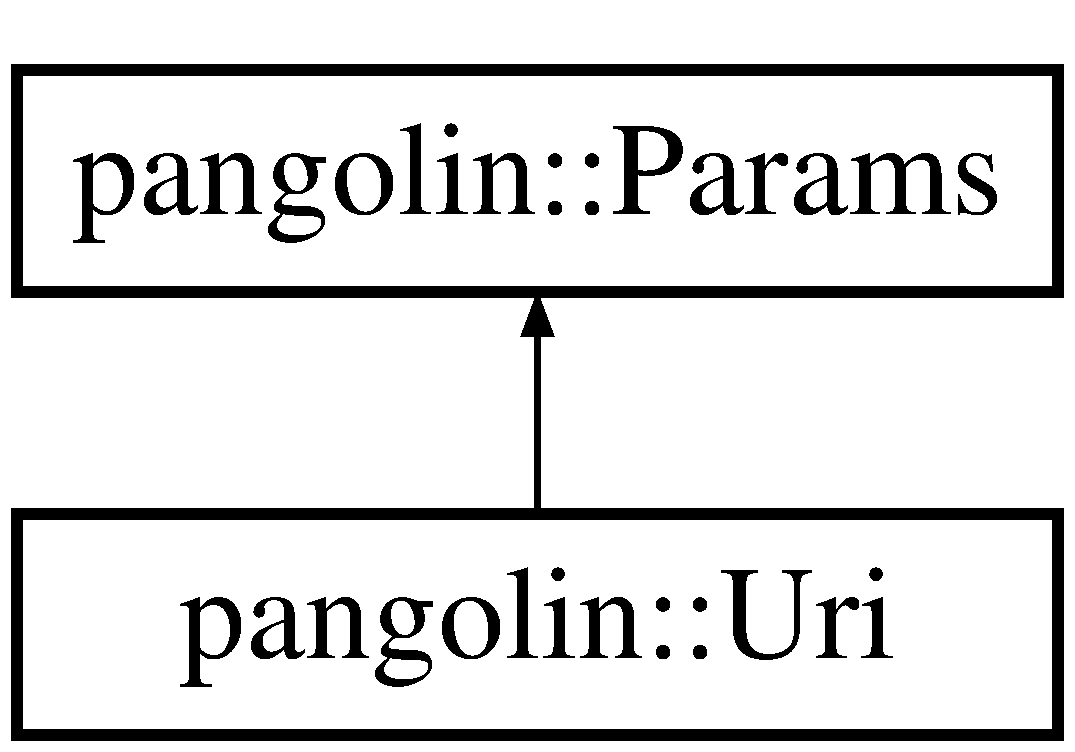
\includegraphics[height=2.000000cm]{classpangolin_1_1_uri}
\end{center}
\end{figure}
\subsection*{Public Attributes}
\begin{DoxyCompactItemize}
\item 
std\+::string {\bfseries scheme}\hypertarget{classpangolin_1_1_uri_a49880799f689f61adb3788e9eef43392}{}\label{classpangolin_1_1_uri_a49880799f689f61adb3788e9eef43392}

\item 
std\+::string {\bfseries url}\hypertarget{classpangolin_1_1_uri_a984fcdc9247f61134c1a40f5662a812e}{}\label{classpangolin_1_1_uri_a984fcdc9247f61134c1a40f5662a812e}

\end{DoxyCompactItemize}
\subsection*{Additional Inherited Members}


The documentation for this class was generated from the following file\+:\begin{DoxyCompactItemize}
\item 
/home/gapo/meng/deps/pangolin/include/pangolin/utils/uri.\+h\end{DoxyCompactItemize}

\hypertarget{classpangolin_1_1_user_app}{}\section{pangolin\+:\+:User\+App Class Reference}
\label{classpangolin_1_1_user_app}\index{pangolin\+::\+User\+App@{pangolin\+::\+User\+App}}
\subsection*{Public Member Functions}
\begin{DoxyCompactItemize}
\item 
virtual void {\bfseries Init} ()\hypertarget{classpangolin_1_1_user_app_abb040aec7a17b8ab2d6a028f89bb4213}{}\label{classpangolin_1_1_user_app_abb040aec7a17b8ab2d6a028f89bb4213}

\item 
virtual void {\bfseries Render} ()=0\hypertarget{classpangolin_1_1_user_app_a772ec714cbbd97530edfe99329879469}{}\label{classpangolin_1_1_user_app_a772ec714cbbd97530edfe99329879469}

\end{DoxyCompactItemize}


The documentation for this class was generated from the following file\+:\begin{DoxyCompactItemize}
\item 
/home/gapo/meng/deps/pangolin/include/pangolin/display/user\+\_\+app.\+h\end{DoxyCompactItemize}

\hypertarget{classpangolin_1_1_uvc_video}{}\section{pangolin\+:\+:Uvc\+Video Class Reference}
\label{classpangolin_1_1_uvc_video}\index{pangolin\+::\+Uvc\+Video@{pangolin\+::\+Uvc\+Video}}
Inheritance diagram for pangolin\+:\+:Uvc\+Video\+:\begin{figure}[H]
\begin{center}
\leavevmode
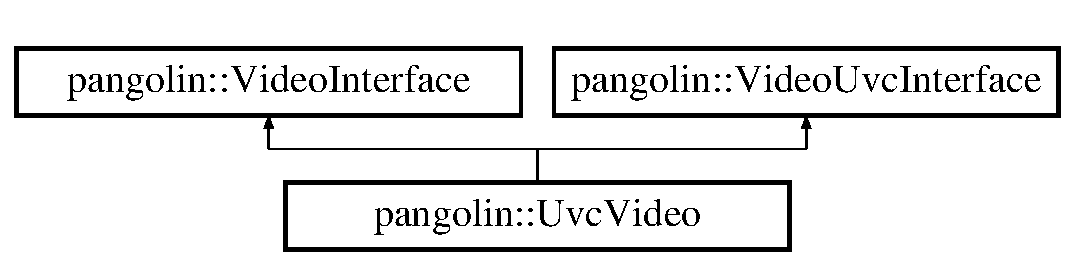
\includegraphics[height=2.000000cm]{classpangolin_1_1_uvc_video}
\end{center}
\end{figure}
\subsection*{Public Member Functions}
\begin{DoxyCompactItemize}
\item 
{\bfseries Uvc\+Video} (int vendor\+\_\+id, int product\+\_\+id, const char $\ast$sn, int deviceid, int width, int height, int fps)\hypertarget{classpangolin_1_1_uvc_video_a0f46c33139437413d96d121f2a28eb8b}{}\label{classpangolin_1_1_uvc_video_a0f46c33139437413d96d121f2a28eb8b}

\item 
void {\bfseries Init\+Device} (int vid, int pid, const char $\ast$sn, int deviceid, int width, int height, int fps)\hypertarget{classpangolin_1_1_uvc_video_a97581ba667b89d4786a7a793a1923f4a}{}\label{classpangolin_1_1_uvc_video_a97581ba667b89d4786a7a793a1923f4a}

\item 
void {\bfseries Deinit\+Device} ()\hypertarget{classpangolin_1_1_uvc_video_a9faed7f02a253bdfa115e46286808f5a}{}\label{classpangolin_1_1_uvc_video_a9faed7f02a253bdfa115e46286808f5a}

\item 
void \hyperlink{classpangolin_1_1_uvc_video_a34accb4f7d75ea6a105cd8002fb54ec9}{Start} ()\hypertarget{classpangolin_1_1_uvc_video_a34accb4f7d75ea6a105cd8002fb54ec9}{}\label{classpangolin_1_1_uvc_video_a34accb4f7d75ea6a105cd8002fb54ec9}

\begin{DoxyCompactList}\small\item\em Implement \hyperlink{structpangolin_1_1_video_input_a74a2e3e1b87c7cbf9de9bcb39e1df128}{Video\+Input\+::\+Start()} \end{DoxyCompactList}\item 
void \hyperlink{classpangolin_1_1_uvc_video_a4650e9189c1f0ac366bece1a1e1b9ecd}{Stop} ()\hypertarget{classpangolin_1_1_uvc_video_a4650e9189c1f0ac366bece1a1e1b9ecd}{}\label{classpangolin_1_1_uvc_video_a4650e9189c1f0ac366bece1a1e1b9ecd}

\begin{DoxyCompactList}\small\item\em Implement \hyperlink{structpangolin_1_1_video_input_a8945f80194cc7ec9594db7f27e7d09b8}{Video\+Input\+::\+Stop()} \end{DoxyCompactList}\item 
size\+\_\+t \hyperlink{classpangolin_1_1_uvc_video_a49b28d342f5200f2cb343493704359d4}{Size\+Bytes} () const \hypertarget{classpangolin_1_1_uvc_video_a49b28d342f5200f2cb343493704359d4}{}\label{classpangolin_1_1_uvc_video_a49b28d342f5200f2cb343493704359d4}

\begin{DoxyCompactList}\small\item\em Implement \hyperlink{structpangolin_1_1_video_input_a93cee5c33386973a2a51165e6bdcf40b}{Video\+Input\+::\+Size\+Bytes()} \end{DoxyCompactList}\item 
const std\+::vector$<$ \hyperlink{classpangolin_1_1_stream_info}{Stream\+Info} $>$ \& \hyperlink{classpangolin_1_1_uvc_video_a265e2dd37db7df5e6494ae97c265a3dd}{Streams} () const \hypertarget{classpangolin_1_1_uvc_video_a265e2dd37db7df5e6494ae97c265a3dd}{}\label{classpangolin_1_1_uvc_video_a265e2dd37db7df5e6494ae97c265a3dd}

\begin{DoxyCompactList}\small\item\em Implement \hyperlink{structpangolin_1_1_video_input_a9030d775d699c39ab7b7ba378c007c6a}{Video\+Input\+::\+Streams()} \end{DoxyCompactList}\item 
bool \hyperlink{classpangolin_1_1_uvc_video_ac78132c9593f8c0dba98b9af38ceded2}{Grab\+Next} (unsigned char $\ast$image, bool wait=true)\hypertarget{classpangolin_1_1_uvc_video_ac78132c9593f8c0dba98b9af38ceded2}{}\label{classpangolin_1_1_uvc_video_ac78132c9593f8c0dba98b9af38ceded2}

\begin{DoxyCompactList}\small\item\em Implement \hyperlink{structpangolin_1_1_video_input_ad3d8ff59c1ec4139320097e6e1111f32}{Video\+Input\+::\+Grab\+Next()} \end{DoxyCompactList}\item 
bool \hyperlink{classpangolin_1_1_uvc_video_a8556f3460309690cdfb99ceeb19ea633}{Grab\+Newest} (unsigned char $\ast$image, bool wait=true)\hypertarget{classpangolin_1_1_uvc_video_a8556f3460309690cdfb99ceeb19ea633}{}\label{classpangolin_1_1_uvc_video_a8556f3460309690cdfb99ceeb19ea633}

\begin{DoxyCompactList}\small\item\em Implement \hyperlink{structpangolin_1_1_video_input_a4c8ac38e3c6a3f591663aeebf645e4c6}{Video\+Input\+::\+Grab\+Newest()} \end{DoxyCompactList}\item 
int \hyperlink{classpangolin_1_1_uvc_video_ae57b7dd563d9894e56ed9f644c4b7998}{Io\+Ctrl} (uint8\+\_\+t unit, uint8\+\_\+t ctrl, unsigned char $\ast$data, int len, Uvc\+Request\+Code req\+\_\+code)\hypertarget{classpangolin_1_1_uvc_video_ae57b7dd563d9894e56ed9f644c4b7998}{}\label{classpangolin_1_1_uvc_video_ae57b7dd563d9894e56ed9f644c4b7998}

\begin{DoxyCompactList}\small\item\em Implement Video\+Uvc\+Interface\+::\+Get\+Ctrl() \end{DoxyCompactList}\end{DoxyCompactItemize}
\subsection*{Static Protected Member Functions}
\begin{DoxyCompactItemize}
\item 
static uvc\+\_\+error\+\_\+t {\bfseries Find\+Device} (uvc\+\_\+context\+\_\+t $\ast$ctx, uvc\+\_\+device\+\_\+t $\ast$$\ast$dev, int vid, int pid, const char $\ast$sn, int device\+\_\+id)\hypertarget{classpangolin_1_1_uvc_video_a7d2cdee6430d09054de1bce4154a8890}{}\label{classpangolin_1_1_uvc_video_a7d2cdee6430d09054de1bce4154a8890}

\end{DoxyCompactItemize}
\subsection*{Protected Attributes}
\begin{DoxyCompactItemize}
\item 
std\+::vector$<$ \hyperlink{classpangolin_1_1_stream_info}{Stream\+Info} $>$ {\bfseries streams}\hypertarget{classpangolin_1_1_uvc_video_a38cc305e8fa109bd62676e81d92a088d}{}\label{classpangolin_1_1_uvc_video_a38cc305e8fa109bd62676e81d92a088d}

\item 
size\+\_\+t {\bfseries size\+\_\+bytes}\hypertarget{classpangolin_1_1_uvc_video_a4496792a1105453f9f0163ba7378b040}{}\label{classpangolin_1_1_uvc_video_a4496792a1105453f9f0163ba7378b040}

\item 
uvc\+\_\+context $\ast$ {\bfseries ctx\+\_\+}\hypertarget{classpangolin_1_1_uvc_video_a2507cb3ebaa50a57fe637c14a2a77f93}{}\label{classpangolin_1_1_uvc_video_a2507cb3ebaa50a57fe637c14a2a77f93}

\item 
uvc\+\_\+device $\ast$ {\bfseries dev\+\_\+}\hypertarget{classpangolin_1_1_uvc_video_a0cd1f79a8eb4ac856c6df7f2246cb887}{}\label{classpangolin_1_1_uvc_video_a0cd1f79a8eb4ac856c6df7f2246cb887}

\item 
uvc\+\_\+device\+\_\+handle $\ast$ {\bfseries devh\+\_\+}\hypertarget{classpangolin_1_1_uvc_video_a104b580732ce02be877f177d88404798}{}\label{classpangolin_1_1_uvc_video_a104b580732ce02be877f177d88404798}

\item 
uvc\+\_\+stream\+\_\+handle $\ast$ {\bfseries strm\+\_\+}\hypertarget{classpangolin_1_1_uvc_video_a266f5101a6fe896555a5ebdfca527bad}{}\label{classpangolin_1_1_uvc_video_a266f5101a6fe896555a5ebdfca527bad}

\item 
uvc\+\_\+stream\+\_\+ctrl\+\_\+t {\bfseries ctrl\+\_\+}\hypertarget{classpangolin_1_1_uvc_video_af4bb68870cabd8abbe1274d5d75ad013}{}\label{classpangolin_1_1_uvc_video_af4bb68870cabd8abbe1274d5d75ad013}

\item 
uvc\+\_\+frame\+\_\+t $\ast$ {\bfseries frame\+\_\+}\hypertarget{classpangolin_1_1_uvc_video_a1793af76ec1ca77dc414c58aa2e575a3}{}\label{classpangolin_1_1_uvc_video_a1793af76ec1ca77dc414c58aa2e575a3}

\end{DoxyCompactItemize}


The documentation for this class was generated from the following file\+:\begin{DoxyCompactItemize}
\item 
/home/gapo/meng/deps/pangolin/include/pangolin/video/drivers/uvc.\+h\end{DoxyCompactItemize}

\hypertarget{classpangolin_1_1_v4l_video}{}\section{pangolin\+:\+:V4l\+Video Class Reference}
\label{classpangolin_1_1_v4l_video}\index{pangolin\+::\+V4l\+Video@{pangolin\+::\+V4l\+Video}}
Inheritance diagram for pangolin\+:\+:V4l\+Video\+:\begin{figure}[H]
\begin{center}
\leavevmode
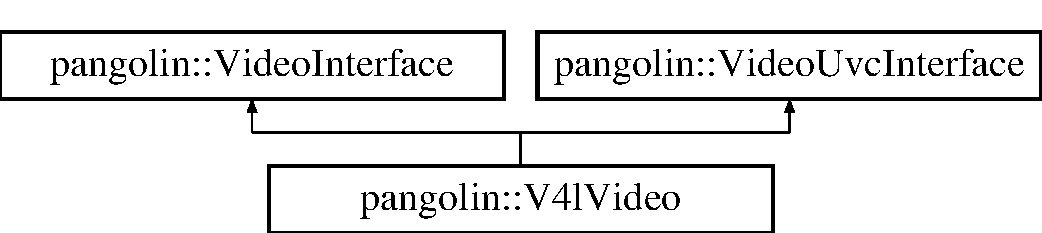
\includegraphics[height=2.000000cm]{classpangolin_1_1_v4l_video}
\end{center}
\end{figure}
\subsection*{Public Member Functions}
\begin{DoxyCompactItemize}
\item 
{\bfseries V4l\+Video} (const char $\ast$dev\+\_\+name, io\+\_\+method io=I\+O\+\_\+\+M\+E\+T\+H\+O\+D\+\_\+\+M\+M\+AP, unsigned iwidth=0, unsigned iheight=0)\hypertarget{classpangolin_1_1_v4l_video_add684f4b5f825d3e9e13dfe4999e00e8}{}\label{classpangolin_1_1_v4l_video_add684f4b5f825d3e9e13dfe4999e00e8}

\item 
void \hyperlink{classpangolin_1_1_v4l_video_a3fde2862c5ae32d61a95d9ed1ec88727}{Start} ()\hypertarget{classpangolin_1_1_v4l_video_a3fde2862c5ae32d61a95d9ed1ec88727}{}\label{classpangolin_1_1_v4l_video_a3fde2862c5ae32d61a95d9ed1ec88727}

\begin{DoxyCompactList}\small\item\em Implement \hyperlink{structpangolin_1_1_video_input_a74a2e3e1b87c7cbf9de9bcb39e1df128}{Video\+Input\+::\+Start()} \end{DoxyCompactList}\item 
void \hyperlink{classpangolin_1_1_v4l_video_a421f6b476a958eaaddccac15f1671dee}{Stop} ()\hypertarget{classpangolin_1_1_v4l_video_a421f6b476a958eaaddccac15f1671dee}{}\label{classpangolin_1_1_v4l_video_a421f6b476a958eaaddccac15f1671dee}

\begin{DoxyCompactList}\small\item\em Implement \hyperlink{structpangolin_1_1_video_input_a8945f80194cc7ec9594db7f27e7d09b8}{Video\+Input\+::\+Stop()} \end{DoxyCompactList}\item 
size\+\_\+t \hyperlink{classpangolin_1_1_v4l_video_ab073c30badb88d77a31f693fe2f1c95f}{Size\+Bytes} () const \hypertarget{classpangolin_1_1_v4l_video_ab073c30badb88d77a31f693fe2f1c95f}{}\label{classpangolin_1_1_v4l_video_ab073c30badb88d77a31f693fe2f1c95f}

\begin{DoxyCompactList}\small\item\em Implement \hyperlink{structpangolin_1_1_video_input_a93cee5c33386973a2a51165e6bdcf40b}{Video\+Input\+::\+Size\+Bytes()} \end{DoxyCompactList}\item 
const std\+::vector$<$ \hyperlink{classpangolin_1_1_stream_info}{Stream\+Info} $>$ \& \hyperlink{classpangolin_1_1_v4l_video_a74fc01f7e4ff5261a760b6a223feead9}{Streams} () const \hypertarget{classpangolin_1_1_v4l_video_a74fc01f7e4ff5261a760b6a223feead9}{}\label{classpangolin_1_1_v4l_video_a74fc01f7e4ff5261a760b6a223feead9}

\begin{DoxyCompactList}\small\item\em Implement \hyperlink{structpangolin_1_1_video_input_a9030d775d699c39ab7b7ba378c007c6a}{Video\+Input\+::\+Streams()} \end{DoxyCompactList}\item 
bool \hyperlink{classpangolin_1_1_v4l_video_aafe3a421c858ab11f170e28ee2a61b61}{Grab\+Next} (unsigned char $\ast$image, bool wait=true)\hypertarget{classpangolin_1_1_v4l_video_aafe3a421c858ab11f170e28ee2a61b61}{}\label{classpangolin_1_1_v4l_video_aafe3a421c858ab11f170e28ee2a61b61}

\begin{DoxyCompactList}\small\item\em Implement \hyperlink{structpangolin_1_1_video_input_ad3d8ff59c1ec4139320097e6e1111f32}{Video\+Input\+::\+Grab\+Next()} \end{DoxyCompactList}\item 
bool \hyperlink{classpangolin_1_1_v4l_video_a3f9c35ccd4a248000cc25c27245d0c75}{Grab\+Newest} (unsigned char $\ast$image, bool wait=true)\hypertarget{classpangolin_1_1_v4l_video_a3f9c35ccd4a248000cc25c27245d0c75}{}\label{classpangolin_1_1_v4l_video_a3f9c35ccd4a248000cc25c27245d0c75}

\begin{DoxyCompactList}\small\item\em Implement \hyperlink{structpangolin_1_1_video_input_a4c8ac38e3c6a3f591663aeebf645e4c6}{Video\+Input\+::\+Grab\+Newest()} \end{DoxyCompactList}\item 
int \hyperlink{classpangolin_1_1_v4l_video_aa5ab2d91f3230a73ed21483874e2bbd0}{Io\+Ctrl} (uint8\+\_\+t unit, uint8\+\_\+t ctrl, unsigned char $\ast$data, int len, Uvc\+Request\+Code req\+\_\+code)\hypertarget{classpangolin_1_1_v4l_video_aa5ab2d91f3230a73ed21483874e2bbd0}{}\label{classpangolin_1_1_v4l_video_aa5ab2d91f3230a73ed21483874e2bbd0}

\begin{DoxyCompactList}\small\item\em Implement Video\+Uvc\+Interface\+::\+Io\+Ctrl() \end{DoxyCompactList}\item 
int {\bfseries Get\+File\+Descriptor} () const \hypertarget{classpangolin_1_1_v4l_video_a609e194ebb94cf48904e94b01cfdf6e2}{}\label{classpangolin_1_1_v4l_video_a609e194ebb94cf48904e94b01cfdf6e2}

\end{DoxyCompactItemize}
\subsection*{Protected Member Functions}
\begin{DoxyCompactItemize}
\item 
int {\bfseries Read\+Frame} (unsigned char $\ast$image)\hypertarget{classpangolin_1_1_v4l_video_aa03b102d989b5015a84ee3e8930fded8}{}\label{classpangolin_1_1_v4l_video_aa03b102d989b5015a84ee3e8930fded8}

\item 
void {\bfseries Mainloop} ()\hypertarget{classpangolin_1_1_v4l_video_a53a08ab6f9b341600b779ef2213e0a6b}{}\label{classpangolin_1_1_v4l_video_a53a08ab6f9b341600b779ef2213e0a6b}

\item 
void {\bfseries init\+\_\+read} (unsigned int buffer\+\_\+size)\hypertarget{classpangolin_1_1_v4l_video_a71e92f409fa13567a937a5e0e77900bf}{}\label{classpangolin_1_1_v4l_video_a71e92f409fa13567a937a5e0e77900bf}

\item 
void {\bfseries init\+\_\+mmap} (const char $\ast$dev\+\_\+name)\hypertarget{classpangolin_1_1_v4l_video_af6c3c40044ee09e50e22fe9cfa728efd}{}\label{classpangolin_1_1_v4l_video_af6c3c40044ee09e50e22fe9cfa728efd}

\item 
void {\bfseries init\+\_\+userp} (const char $\ast$dev\+\_\+name, unsigned int buffer\+\_\+size)\hypertarget{classpangolin_1_1_v4l_video_a2539b07bc8d2fde5a1a9aa07cc85d180}{}\label{classpangolin_1_1_v4l_video_a2539b07bc8d2fde5a1a9aa07cc85d180}

\item 
void {\bfseries init\+\_\+device} (const char $\ast$dev\+\_\+name, unsigned iwidth, unsigned iheight, unsigned ifps, unsigned v4l\+\_\+format=V4\+L2\+\_\+\+P\+I\+X\+\_\+\+F\+M\+T\+\_\+\+Y\+U\+YV, v4l2\+\_\+field field=V4\+L2\+\_\+\+F\+I\+E\+L\+D\+\_\+\+I\+N\+T\+E\+R\+L\+A\+C\+ED)\hypertarget{classpangolin_1_1_v4l_video_a92835b5adcb2c00902be4f4556a0a9a6}{}\label{classpangolin_1_1_v4l_video_a92835b5adcb2c00902be4f4556a0a9a6}

\item 
void {\bfseries uninit\+\_\+device} ()\hypertarget{classpangolin_1_1_v4l_video_a6bb2b253d94bb0e6e6af51c452df4df3}{}\label{classpangolin_1_1_v4l_video_a6bb2b253d94bb0e6e6af51c452df4df3}

\item 
void {\bfseries open\+\_\+device} (const char $\ast$dev\+\_\+name)\hypertarget{classpangolin_1_1_v4l_video_a40328a5e2bbe793fcf81445b7b2dc668}{}\label{classpangolin_1_1_v4l_video_a40328a5e2bbe793fcf81445b7b2dc668}

\item 
void {\bfseries close\+\_\+device} ()\hypertarget{classpangolin_1_1_v4l_video_a6e8663c9e310c200f93130a80993409c}{}\label{classpangolin_1_1_v4l_video_a6e8663c9e310c200f93130a80993409c}

\end{DoxyCompactItemize}
\subsection*{Protected Attributes}
\begin{DoxyCompactItemize}
\item 
std\+::vector$<$ \hyperlink{classpangolin_1_1_stream_info}{Stream\+Info} $>$ {\bfseries streams}\hypertarget{classpangolin_1_1_v4l_video_a9771b87a27ad851fa81ea13768eda966}{}\label{classpangolin_1_1_v4l_video_a9771b87a27ad851fa81ea13768eda966}

\item 
io\+\_\+method {\bfseries io}\hypertarget{classpangolin_1_1_v4l_video_aafa59444a2b911df8683f842c1feaba8}{}\label{classpangolin_1_1_v4l_video_aafa59444a2b911df8683f842c1feaba8}

\item 
int {\bfseries fd}\hypertarget{classpangolin_1_1_v4l_video_a3bb336b39aadbaade92198a8f7a5b1ce}{}\label{classpangolin_1_1_v4l_video_a3bb336b39aadbaade92198a8f7a5b1ce}

\item 
\hyperlink{structpangolin_1_1buffer}{buffer} $\ast$ {\bfseries buffers}\hypertarget{classpangolin_1_1_v4l_video_ac0a8f37b6d928847a2c968627eec7b7c}{}\label{classpangolin_1_1_v4l_video_ac0a8f37b6d928847a2c968627eec7b7c}

\item 
unsigned int {\bfseries n\+\_\+buffers}\hypertarget{classpangolin_1_1_v4l_video_a3d9daca852997941b524c3856fb30b5a}{}\label{classpangolin_1_1_v4l_video_a3d9daca852997941b524c3856fb30b5a}

\item 
bool {\bfseries running}\hypertarget{classpangolin_1_1_v4l_video_a9e873d28ed7d80dc3648b53137f77e9c}{}\label{classpangolin_1_1_v4l_video_a9e873d28ed7d80dc3648b53137f77e9c}

\item 
unsigned {\bfseries width}\hypertarget{classpangolin_1_1_v4l_video_af880ba8871b91b0b020c06273c5b652f}{}\label{classpangolin_1_1_v4l_video_af880ba8871b91b0b020c06273c5b652f}

\item 
unsigned {\bfseries height}\hypertarget{classpangolin_1_1_v4l_video_a57945faa1eb9b8f63a93e2fccb149676}{}\label{classpangolin_1_1_v4l_video_a57945faa1eb9b8f63a93e2fccb149676}

\item 
float {\bfseries fps}\hypertarget{classpangolin_1_1_v4l_video_a97797118cb7532f10008ca36eab1a56a}{}\label{classpangolin_1_1_v4l_video_a97797118cb7532f10008ca36eab1a56a}

\item 
size\+\_\+t {\bfseries image\+\_\+size}\hypertarget{classpangolin_1_1_v4l_video_abfca1d79f922b7f66935c857a61143aa}{}\label{classpangolin_1_1_v4l_video_abfca1d79f922b7f66935c857a61143aa}

\end{DoxyCompactItemize}


The documentation for this class was generated from the following file\+:\begin{DoxyCompactItemize}
\item 
/home/gapo/meng/deps/pangolin/include/pangolin/video/drivers/v4l.\+h\end{DoxyCompactItemize}

\hypertarget{classpangolin_1_1json_1_1value}{}\section{pangolin\+:\+:json\+:\+:value Class Reference}
\label{classpangolin_1_1json_1_1value}\index{pangolin\+::json\+::value@{pangolin\+::json\+::value}}
\subsection*{Classes}
\begin{DoxyCompactItemize}
\item 
union \hyperlink{unionpangolin_1_1json_1_1value_1_1__storage}{\+\_\+storage}
\end{DoxyCompactItemize}
\subsection*{Public Types}
\begin{DoxyCompactItemize}
\item 
typedef std\+::vector$<$ \hyperlink{classpangolin_1_1json_1_1value}{value} $>$ {\bfseries array}\hypertarget{classpangolin_1_1json_1_1value_a3b2da03c1d45779ad4035f4178ccd804}{}\label{classpangolin_1_1json_1_1value_a3b2da03c1d45779ad4035f4178ccd804}

\item 
typedef std\+::map$<$ std\+::string, \hyperlink{classpangolin_1_1json_1_1value}{value} $>$ {\bfseries object}\hypertarget{classpangolin_1_1json_1_1value_a6dd5198699e330c2c8b5564c99586cc1}{}\label{classpangolin_1_1json_1_1value_a6dd5198699e330c2c8b5564c99586cc1}

\end{DoxyCompactItemize}
\subsection*{Public Member Functions}
\begin{DoxyCompactItemize}
\item 
{\bfseries value} (int type, bool)\hypertarget{classpangolin_1_1json_1_1value_a5eacf26a4b7f8099366e19f2cb0f64a5}{}\label{classpangolin_1_1json_1_1value_a5eacf26a4b7f8099366e19f2cb0f64a5}

\item 
{\bfseries value} (bool b)\hypertarget{classpangolin_1_1json_1_1value_a372c0bb1d79a7b8e6312899debc1245d}{}\label{classpangolin_1_1json_1_1value_a372c0bb1d79a7b8e6312899debc1245d}

\item 
{\bfseries value} (short v)\hypertarget{classpangolin_1_1json_1_1value_a53c8eefb0df4964a4f5d765f191a2956}{}\label{classpangolin_1_1json_1_1value_a53c8eefb0df4964a4f5d765f191a2956}

\item 
{\bfseries value} (unsigned short v)\hypertarget{classpangolin_1_1json_1_1value_a8aa58b0259f8971e04ff6eab35d28591}{}\label{classpangolin_1_1json_1_1value_a8aa58b0259f8971e04ff6eab35d28591}

\item 
{\bfseries value} (int v)\hypertarget{classpangolin_1_1json_1_1value_a2883830cd70040c8abe199ecd2709a5b}{}\label{classpangolin_1_1json_1_1value_a2883830cd70040c8abe199ecd2709a5b}

\item 
{\bfseries value} (unsigned int v)\hypertarget{classpangolin_1_1json_1_1value_aeb0adaa5ffc03f176aac712c75020824}{}\label{classpangolin_1_1json_1_1value_aeb0adaa5ffc03f176aac712c75020824}

\item 
{\bfseries value} (long v)\hypertarget{classpangolin_1_1json_1_1value_a3ae20b7008a89a960e79781a1eb5fe28}{}\label{classpangolin_1_1json_1_1value_a3ae20b7008a89a960e79781a1eb5fe28}

\item 
{\bfseries value} (unsigned long v)\hypertarget{classpangolin_1_1json_1_1value_a2c89b26dc42112c0e17af8fdbc64edce}{}\label{classpangolin_1_1json_1_1value_a2c89b26dc42112c0e17af8fdbc64edce}

\item 
{\bfseries value} (long long v)\hypertarget{classpangolin_1_1json_1_1value_a962207e830534cc31bbba245d99e67c8}{}\label{classpangolin_1_1json_1_1value_a962207e830534cc31bbba245d99e67c8}

\item 
{\bfseries value} (unsigned long long v)\hypertarget{classpangolin_1_1json_1_1value_af73df6f40c73af3ad90dbd8068274d1f}{}\label{classpangolin_1_1json_1_1value_af73df6f40c73af3ad90dbd8068274d1f}

\item 
{\bfseries value} (float n)\hypertarget{classpangolin_1_1json_1_1value_ab2a007a0bfbc8282e9f58f81d512844b}{}\label{classpangolin_1_1json_1_1value_ab2a007a0bfbc8282e9f58f81d512844b}

\item 
{\bfseries value} (double n)\hypertarget{classpangolin_1_1json_1_1value_a46b6b3ab078b2f8ed52644553423f7bd}{}\label{classpangolin_1_1json_1_1value_a46b6b3ab078b2f8ed52644553423f7bd}

\item 
{\bfseries value} (const array \&a)\hypertarget{classpangolin_1_1json_1_1value_a14376ede7c7122120637cf181e9c8f34}{}\label{classpangolin_1_1json_1_1value_a14376ede7c7122120637cf181e9c8f34}

\item 
{\bfseries value} (const object \&o)\hypertarget{classpangolin_1_1json_1_1value_a130f6e710eb8cf63383c537ceb26c936}{}\label{classpangolin_1_1json_1_1value_a130f6e710eb8cf63383c537ceb26c936}

\item 
{\bfseries value} (const std\+::string \&s)\hypertarget{classpangolin_1_1json_1_1value_adafb3869509a66ad622953961fb3c199}{}\label{classpangolin_1_1json_1_1value_adafb3869509a66ad622953961fb3c199}

\item 
{\bfseries value} (const char $\ast$s)\hypertarget{classpangolin_1_1json_1_1value_afde8d19003c9f8a7796a0dae728f1e9a}{}\label{classpangolin_1_1json_1_1value_afde8d19003c9f8a7796a0dae728f1e9a}

\item 
{\bfseries value} (const char $\ast$s, size\+\_\+t len)\hypertarget{classpangolin_1_1json_1_1value_ae2b8a3f25b95012c29d45ce8032ac566}{}\label{classpangolin_1_1json_1_1value_ae2b8a3f25b95012c29d45ce8032ac566}

\item 
{\bfseries value} (const \hyperlink{classpangolin_1_1json_1_1value}{value} \&x)\hypertarget{classpangolin_1_1json_1_1value_a61479ed7b7e2ededb89353c1c051b7ae}{}\label{classpangolin_1_1json_1_1value_a61479ed7b7e2ededb89353c1c051b7ae}

\item 
\hyperlink{classpangolin_1_1json_1_1value}{value} \& {\bfseries operator=} (const \hyperlink{classpangolin_1_1json_1_1value}{value} \&x)\hypertarget{classpangolin_1_1json_1_1value_a414a3bae51895cdde61641e05e93e7be}{}\label{classpangolin_1_1json_1_1value_a414a3bae51895cdde61641e05e93e7be}

\item 
void {\bfseries swap} (\hyperlink{classpangolin_1_1json_1_1value}{value} \&x)\hypertarget{classpangolin_1_1json_1_1value_aaf64e14a2af6864ac6ffaabca752d025}{}\label{classpangolin_1_1json_1_1value_aaf64e14a2af6864ac6ffaabca752d025}

\item 
{\footnotesize template$<$typename T $>$ }\\bool {\bfseries is} () const \hypertarget{classpangolin_1_1json_1_1value_abac38be098c094e64cbb53cccd04866e}{}\label{classpangolin_1_1json_1_1value_abac38be098c094e64cbb53cccd04866e}

\item 
{\footnotesize template$<$typename T $>$ }\\const T \& {\bfseries get} () const \hypertarget{classpangolin_1_1json_1_1value_a86fadab0278acc0919e891282ad450e1}{}\label{classpangolin_1_1json_1_1value_a86fadab0278acc0919e891282ad450e1}

\item 
{\footnotesize template$<$typename T $>$ }\\T \& {\bfseries get} ()\hypertarget{classpangolin_1_1json_1_1value_a7292113142d8cf02d2b389937ff16e02}{}\label{classpangolin_1_1json_1_1value_a7292113142d8cf02d2b389937ff16e02}

\item 
bool {\bfseries evaluate\+\_\+as\+\_\+boolean} () const \hypertarget{classpangolin_1_1json_1_1value_a36613acd0d644c2bca1618bdfc6d3ff6}{}\label{classpangolin_1_1json_1_1value_a36613acd0d644c2bca1618bdfc6d3ff6}

\item 
size\+\_\+t {\bfseries size} () const \hypertarget{classpangolin_1_1json_1_1value_a64eea04ca16d3be156aae8a3d75a1245}{}\label{classpangolin_1_1json_1_1value_a64eea04ca16d3be156aae8a3d75a1245}

\item 
\hyperlink{classpangolin_1_1json_1_1value}{value} \& {\bfseries operator\mbox{[}$\,$\mbox{]}} (size\+\_\+t idx)\hypertarget{classpangolin_1_1json_1_1value_a2fd1d1e12b280502c1d7a0830a980e0b}{}\label{classpangolin_1_1json_1_1value_a2fd1d1e12b280502c1d7a0830a980e0b}

\item 
const \hyperlink{classpangolin_1_1json_1_1value}{value} \& {\bfseries operator\mbox{[}$\,$\mbox{]}} (size\+\_\+t idx) const \hypertarget{classpangolin_1_1json_1_1value_a27799bda0c2c9f5d9179c74fe3e6cfb4}{}\label{classpangolin_1_1json_1_1value_a27799bda0c2c9f5d9179c74fe3e6cfb4}

\item 
bool {\bfseries contains} (size\+\_\+t idx) const \hypertarget{classpangolin_1_1json_1_1value_a5e5ae3536574540261765ec421f11370}{}\label{classpangolin_1_1json_1_1value_a5e5ae3536574540261765ec421f11370}

\item 
\hyperlink{classpangolin_1_1json_1_1value}{value} \& {\bfseries push\+\_\+back} (const \hyperlink{classpangolin_1_1json_1_1value}{value} \&=\hyperlink{classpangolin_1_1json_1_1value}{value}())\hypertarget{classpangolin_1_1json_1_1value_a2640589bacc1f4d2d840e8e869d9938b}{}\label{classpangolin_1_1json_1_1value_a2640589bacc1f4d2d840e8e869d9938b}

\item 
\hyperlink{classpangolin_1_1json_1_1value}{value} \& {\bfseries operator\mbox{[}$\,$\mbox{]}} (const std\+::string \&key)\hypertarget{classpangolin_1_1json_1_1value_ad6b5b6871a43ca2f3c17e33886a528e2}{}\label{classpangolin_1_1json_1_1value_ad6b5b6871a43ca2f3c17e33886a528e2}

\item 
const \hyperlink{classpangolin_1_1json_1_1value}{value} \& {\bfseries operator\mbox{[}$\,$\mbox{]}} (const std\+::string \&key) const \hypertarget{classpangolin_1_1json_1_1value_a9ab171bf0f42ec8b1330f987acfe52de}{}\label{classpangolin_1_1json_1_1value_a9ab171bf0f42ec8b1330f987acfe52de}

\item 
bool {\bfseries contains} (const std\+::string \&key) const \hypertarget{classpangolin_1_1json_1_1value_a1a1865bacd4995520faf4f990ce11c37}{}\label{classpangolin_1_1json_1_1value_a1a1865bacd4995520faf4f990ce11c37}

\item 
std\+::string {\bfseries to\+\_\+str} () const \hypertarget{classpangolin_1_1json_1_1value_aed94ac9f62ad997a5cb6e391bceda4c8}{}\label{classpangolin_1_1json_1_1value_aed94ac9f62ad997a5cb6e391bceda4c8}

\item 
{\footnotesize template$<$typename Iter $>$ }\\void {\bfseries serialize} (Iter os, bool prettify=false) const \hypertarget{classpangolin_1_1json_1_1value_ac409f37643ce8870949a16340e37a31c}{}\label{classpangolin_1_1json_1_1value_ac409f37643ce8870949a16340e37a31c}

\item 
std\+::string {\bfseries serialize} (bool prettify=false) const \hypertarget{classpangolin_1_1json_1_1value_a94df9fd155f49827a1f68d2aea6f16e8}{}\label{classpangolin_1_1json_1_1value_a94df9fd155f49827a1f68d2aea6f16e8}

\item 
{\footnotesize template$<$$>$ }\\bool {\bfseries is} () const \hypertarget{classpangolin_1_1json_1_1value_a651152b67ff55a21e399655d8c52c105}{}\label{classpangolin_1_1json_1_1value_a651152b67ff55a21e399655d8c52c105}

\end{DoxyCompactItemize}
\subsection*{Protected Attributes}
\begin{DoxyCompactItemize}
\item 
int {\bfseries type\+\_\+}\hypertarget{classpangolin_1_1json_1_1value_ac72be5858ea55ef2b54815b70856d56e}{}\label{classpangolin_1_1json_1_1value_ac72be5858ea55ef2b54815b70856d56e}

\item 
\hyperlink{unionpangolin_1_1json_1_1value_1_1__storage}{\+\_\+storage} {\bfseries u\+\_\+}\hypertarget{classpangolin_1_1json_1_1value_aed6388e301197199b6ff01e9aaef27ce}{}\label{classpangolin_1_1json_1_1value_aed6388e301197199b6ff01e9aaef27ce}

\end{DoxyCompactItemize}


The documentation for this class was generated from the following file\+:\begin{DoxyCompactItemize}
\item 
/home/gapo/meng/deps/pangolin/include/pangolin/utils/picojson.\+h\end{DoxyCompactItemize}

\hypertarget{classpangolin_1_1_var}{}\section{pangolin\+:\+:Var$<$ T $>$ Class Template Reference}
\label{classpangolin_1_1_var}\index{pangolin\+::\+Var$<$ T $>$@{pangolin\+::\+Var$<$ T $>$}}
Inheritance diagram for pangolin\+:\+:Var$<$ T $>$\+:\begin{figure}[H]
\begin{center}
\leavevmode
\includegraphics[height=2.000000cm]{classpangolin_1_1_var}
\end{center}
\end{figure}
\subsection*{Public Member Functions}
\begin{DoxyCompactItemize}
\item 
{\bfseries Var} (\hyperlink{classpangolin_1_1_var_value_generic}{Var\+Value\+Generic} \&v)\hypertarget{classpangolin_1_1_var_aef05c02cdfa656eb66f7d111c4d6e398}{}\label{classpangolin_1_1_var_aef05c02cdfa656eb66f7d111c4d6e398}

\item 
{\bfseries Var} (const std\+::string \&name)\hypertarget{classpangolin_1_1_var_af933d913b9a26a1c826c459238419e45}{}\label{classpangolin_1_1_var_af933d913b9a26a1c826c459238419e45}

\item 
{\bfseries Var} (const std\+::string \&name, const T \&value, bool toggle=false)\hypertarget{classpangolin_1_1_var_ac5baae380efb22a80ada9b08263629dd}{}\label{classpangolin_1_1_var_ac5baae380efb22a80ada9b08263629dd}

\item 
{\bfseries Var} (const std\+::string \&name, const T \&value, double min, double max, bool logscale=false)\hypertarget{classpangolin_1_1_var_a6b0fa35641988e3a73c0c637779021e9}{}\label{classpangolin_1_1_var_a6b0fa35641988e3a73c0c637779021e9}

\item 
void {\bfseries Reset} ()\hypertarget{classpangolin_1_1_var_a9451def521ef050d504de505c0873181}{}\label{classpangolin_1_1_var_a9451def521ef050d504de505c0873181}

\item 
const T \& {\bfseries Get} ()\hypertarget{classpangolin_1_1_var_a842d2c0de45c54d0e28cf4d4a2d3750d}{}\label{classpangolin_1_1_var_a842d2c0de45c54d0e28cf4d4a2d3750d}

\item 
{\bfseries operator const T \&} ()\hypertarget{classpangolin_1_1_var_aab2a781db067c25a9dbc1d43eb0437df}{}\label{classpangolin_1_1_var_aab2a781db067c25a9dbc1d43eb0437df}

\item 
const T $\ast$ {\bfseries operator-\/$>$} ()\hypertarget{classpangolin_1_1_var_aa3a881d3345d70f8c22eb5f418e21650}{}\label{classpangolin_1_1_var_aa3a881d3345d70f8c22eb5f418e21650}

\item 
void {\bfseries operator=} (const T \&val)\hypertarget{classpangolin_1_1_var_a4c14268bb925bfaacf1c8ac338b8d170}{}\label{classpangolin_1_1_var_a4c14268bb925bfaacf1c8ac338b8d170}

\item 
void {\bfseries operator=} (const \hyperlink{classpangolin_1_1_var}{Var}$<$ T $>$ \&v)\hypertarget{classpangolin_1_1_var_a653604048343123abb364356348dfb9e}{}\label{classpangolin_1_1_var_a653604048343123abb364356348dfb9e}

\item 
\hyperlink{structpangolin_1_1_var_meta}{Var\+Meta} \& {\bfseries Meta} ()\hypertarget{classpangolin_1_1_var_a200ac286e880eb3ef6d815b742448c6e}{}\label{classpangolin_1_1_var_a200ac286e880eb3ef6d815b742448c6e}

\item 
bool {\bfseries Gui\+Changed} ()\hypertarget{classpangolin_1_1_var_ae8cf8e2f9df55e36d7a14b5033157d6d}{}\label{classpangolin_1_1_var_ae8cf8e2f9df55e36d7a14b5033157d6d}

\item 
\hyperlink{classpangolin_1_1_var_value_t}{Var\+ValueT}$<$ T $>$ \& {\bfseries Ref} ()\hypertarget{classpangolin_1_1_var_a3989d6eb6a1d2fb373e0510a97bbb339}{}\label{classpangolin_1_1_var_a3989d6eb6a1d2fb373e0510a97bbb339}

\end{DoxyCompactItemize}
\subsection*{Static Public Member Functions}
\begin{DoxyCompactItemize}
\item 
static void {\bfseries Attach} (const std\+::string \&name, T \&variable, double min, double max, bool logscale=false)\hypertarget{classpangolin_1_1_var_a1568007fddbc4d22009d303419769f51}{}\label{classpangolin_1_1_var_a1568007fddbc4d22009d303419769f51}

\item 
static void {\bfseries Attach} (const std\+::string \&name, T \&variable, bool toggle=false)\hypertarget{classpangolin_1_1_var_a5311bec43d936d9e6d967a6bf7264446}{}\label{classpangolin_1_1_var_a5311bec43d936d9e6d967a6bf7264446}

\end{DoxyCompactItemize}
\subsection*{Protected Member Functions}
\begin{DoxyCompactItemize}
\item 
void {\bfseries Initialise\+From\+Generic} (\hyperlink{classpangolin_1_1_var_value_generic}{Var\+Value\+Generic} $\ast$v)\hypertarget{classpangolin_1_1_var_af003420edf68489edea89e958e4bb7eb}{}\label{classpangolin_1_1_var_af003420edf68489edea89e958e4bb7eb}

\end{DoxyCompactItemize}
\subsection*{Protected Attributes}
\begin{DoxyCompactItemize}
\item 
\hyperlink{classpangolin_1_1_var_value_t}{Var\+ValueT}$<$ T $>$ $\ast$ {\bfseries var}\hypertarget{classpangolin_1_1_var_ae40747fbc28ddcb3ac47a0cd60ba1b7c}{}\label{classpangolin_1_1_var_ae40747fbc28ddcb3ac47a0cd60ba1b7c}

\item 
\hyperlink{classpangolin_1_1_var_value_t}{Var\+ValueT}$<$ T $>$ $\ast$ {\bfseries ptr}\hypertarget{classpangolin_1_1_var_adc45d72e50bbc3bf652c8a1d64eaa388}{}\label{classpangolin_1_1_var_adc45d72e50bbc3bf652c8a1d64eaa388}

\end{DoxyCompactItemize}


The documentation for this class was generated from the following file\+:\begin{DoxyCompactItemize}
\item 
/home/gapo/meng/deps/pangolin/include/pangolin/var/var.\+h\end{DoxyCompactItemize}

\hypertarget{structpangolin_1_1_var_meta}{}\section{pangolin\+:\+:Var\+Meta Struct Reference}
\label{structpangolin_1_1_var_meta}\index{pangolin\+::\+Var\+Meta@{pangolin\+::\+Var\+Meta}}
\subsection*{Public Attributes}
\begin{DoxyCompactItemize}
\item 
std\+::string {\bfseries full\+\_\+name}\hypertarget{structpangolin_1_1_var_meta_aaa7c74e619c399ea1d0774984d6bc774}{}\label{structpangolin_1_1_var_meta_aaa7c74e619c399ea1d0774984d6bc774}

\item 
std\+::string {\bfseries friendly}\hypertarget{structpangolin_1_1_var_meta_a3fbadd6262c30451c0e54a437362bcd2}{}\label{structpangolin_1_1_var_meta_a3fbadd6262c30451c0e54a437362bcd2}

\item 
double {\bfseries range} \mbox{[}2\mbox{]}\hypertarget{structpangolin_1_1_var_meta_a9a3d4262dae0dd8292a106dfaf8302f0}{}\label{structpangolin_1_1_var_meta_a9a3d4262dae0dd8292a106dfaf8302f0}

\item 
double {\bfseries increment}\hypertarget{structpangolin_1_1_var_meta_a2666e59d58a614c09faad95cca9fc650}{}\label{structpangolin_1_1_var_meta_a2666e59d58a614c09faad95cca9fc650}

\item 
int {\bfseries flags}\hypertarget{structpangolin_1_1_var_meta_a83d177e52526b210bffbba93cc1755b8}{}\label{structpangolin_1_1_var_meta_a83d177e52526b210bffbba93cc1755b8}

\item 
bool {\bfseries gui\+\_\+changed}\hypertarget{structpangolin_1_1_var_meta_a92e78c771a66c500dd901c4b76738569}{}\label{structpangolin_1_1_var_meta_a92e78c771a66c500dd901c4b76738569}

\item 
bool {\bfseries logscale}\hypertarget{structpangolin_1_1_var_meta_a26c9a8af4a6cc5842f70a7e8c7123580}{}\label{structpangolin_1_1_var_meta_a26c9a8af4a6cc5842f70a7e8c7123580}

\item 
bool {\bfseries generic}\hypertarget{structpangolin_1_1_var_meta_a110148551c546e95c63e537bb13bb30b}{}\label{structpangolin_1_1_var_meta_a110148551c546e95c63e537bb13bb30b}

\end{DoxyCompactItemize}


The documentation for this struct was generated from the following file\+:\begin{DoxyCompactItemize}
\item 
/home/gapo/meng/deps/pangolin/include/pangolin/var/varvaluegeneric.\+h\end{DoxyCompactItemize}

\hypertarget{classpangolin_1_1_var_state}{}\section{pangolin\+:\+:Var\+State Class Reference}
\label{classpangolin_1_1_var_state}\index{pangolin\+::\+Var\+State@{pangolin\+::\+Var\+State}}
\subsection*{Public Types}
\begin{DoxyCompactItemize}
\item 
typedef std\+::map$<$ std\+::string, \hyperlink{classpangolin_1_1_var_value_generic}{Var\+Value\+Generic} $\ast$ $>$ {\bfseries Var\+Store\+Container}\hypertarget{classpangolin_1_1_var_state_a4b0f4490d5a2d774355568abab604827}{}\label{classpangolin_1_1_var_state_a4b0f4490d5a2d774355568abab604827}

\item 
typedef std\+::vector$<$ std\+::string $>$ {\bfseries Var\+Store\+Additions}\hypertarget{classpangolin_1_1_var_state_a83362aae7d05747448cd0caa039b5d0a}{}\label{classpangolin_1_1_var_state_a83362aae7d05747448cd0caa039b5d0a}

\end{DoxyCompactItemize}
\subsection*{Public Member Functions}
\begin{DoxyCompactItemize}
\item 
void {\bfseries Clear} ()\hypertarget{classpangolin_1_1_var_state_a2345876a86667af235fbfcd34d592765}{}\label{classpangolin_1_1_var_state_a2345876a86667af235fbfcd34d592765}

\item 
{\footnotesize template$<$typename T $>$ }\\void {\bfseries Notify\+New\+Var} (const std\+::string \&name, \hyperlink{classpangolin_1_1_var_value}{Var\+Value}$<$ T $>$ \&var)\hypertarget{classpangolin_1_1_var_state_a0c46301ad04fd79b3d39cf4aad06a27b}{}\label{classpangolin_1_1_var_state_a0c46301ad04fd79b3d39cf4aad06a27b}

\item 
\hyperlink{classpangolin_1_1_var_value_generic}{Var\+Value\+Generic} $\ast$\& {\bfseries operator\mbox{[}$\,$\mbox{]}} (const std\+::string \&str)\hypertarget{classpangolin_1_1_var_state_a7c47b668551ba9bec79af99417fbd22a}{}\label{classpangolin_1_1_var_state_a7c47b668551ba9bec79af99417fbd22a}

\item 
bool {\bfseries Exists} (const std\+::string \&str) const \hypertarget{classpangolin_1_1_var_state_ac1cb727a005c19f064512a707ff21ff6}{}\label{classpangolin_1_1_var_state_ac1cb727a005c19f064512a707ff21ff6}

\end{DoxyCompactItemize}
\subsection*{Static Public Member Functions}
\begin{DoxyCompactItemize}
\item 
static \hyperlink{classpangolin_1_1_var_state}{Var\+State} \& {\bfseries I} ()\hypertarget{classpangolin_1_1_var_state_aa7d02f377798c62f7669b81662acd0bc}{}\label{classpangolin_1_1_var_state_aa7d02f377798c62f7669b81662acd0bc}

\end{DoxyCompactItemize}
\subsection*{Public Attributes}
\begin{DoxyCompactItemize}
\item 
Var\+Store\+Container {\bfseries vars}\hypertarget{classpangolin_1_1_var_state_ac3b9cb32a9c9781e3d9bc8fbdaa8392b}{}\label{classpangolin_1_1_var_state_ac3b9cb32a9c9781e3d9bc8fbdaa8392b}

\item 
Var\+Store\+Additions {\bfseries var\+\_\+adds}\hypertarget{classpangolin_1_1_var_state_a6c13d1b6ae71a520ec272fca48917027}{}\label{classpangolin_1_1_var_state_a6c13d1b6ae71a520ec272fca48917027}

\item 
std\+::vector$<$ \hyperlink{structpangolin_1_1_new_var_callback}{New\+Var\+Callback} $>$ {\bfseries new\+\_\+var\+\_\+callbacks}\hypertarget{classpangolin_1_1_var_state_ac1af07eb2736ca373b344068f9fe702c}{}\label{classpangolin_1_1_var_state_ac1af07eb2736ca373b344068f9fe702c}

\item 
std\+::vector$<$ \hyperlink{structpangolin_1_1_gui_var_changed_callback}{Gui\+Var\+Changed\+Callback} $>$ {\bfseries gui\+\_\+var\+\_\+changed\+\_\+callbacks}\hypertarget{classpangolin_1_1_var_state_ac01d31cc1ea6943fc81cb7f0778070bb}{}\label{classpangolin_1_1_var_state_ac01d31cc1ea6943fc81cb7f0778070bb}

\end{DoxyCompactItemize}


The documentation for this class was generated from the following file\+:\begin{DoxyCompactItemize}
\item 
/home/gapo/meng/deps/pangolin/include/pangolin/var/varstate.\+h\end{DoxyCompactItemize}

\hypertarget{classpangolin_1_1_var_value}{}\section{pangolin\+:\+:Var\+Value$<$ T $>$ Class Template Reference}
\label{classpangolin_1_1_var_value}\index{pangolin\+::\+Var\+Value$<$ T $>$@{pangolin\+::\+Var\+Value$<$ T $>$}}
Inheritance diagram for pangolin\+:\+:Var\+Value$<$ T $>$\+:\begin{figure}[H]
\begin{center}
\leavevmode
\includegraphics[height=3.000000cm]{classpangolin_1_1_var_value}
\end{center}
\end{figure}
\subsection*{Public Types}
\begin{DoxyCompactItemize}
\item 
typedef boostd\+::remove\+\_\+reference$<$ T $>$\+::type {\bfseries VarT}\hypertarget{classpangolin_1_1_var_value_aa1822b992c750c2a08eeb4fb5e1162b0}{}\label{classpangolin_1_1_var_value_aa1822b992c750c2a08eeb4fb5e1162b0}

\end{DoxyCompactItemize}
\subsection*{Public Member Functions}
\begin{DoxyCompactItemize}
\item 
{\bfseries Var\+Value} (const T \&value)\hypertarget{classpangolin_1_1_var_value_a40b682384d10b19f0ce5621988f86745}{}\label{classpangolin_1_1_var_value_a40b682384d10b19f0ce5621988f86745}

\item 
{\bfseries Var\+Value} (const T \&value, const VarT \&default\+\_\+value)\hypertarget{classpangolin_1_1_var_value_aed1387627a75f1eeb290793484ba72a3}{}\label{classpangolin_1_1_var_value_aed1387627a75f1eeb290793484ba72a3}

\item 
const char $\ast$ {\bfseries Type\+Id} () const \hypertarget{classpangolin_1_1_var_value_ae4a3ef3daea7d4944c0acfe959dd9a31}{}\label{classpangolin_1_1_var_value_ae4a3ef3daea7d4944c0acfe959dd9a31}

\item 
void {\bfseries Reset} ()\hypertarget{classpangolin_1_1_var_value_a23d1da24e04e208b001890a8306dc19b}{}\label{classpangolin_1_1_var_value_a23d1da24e04e208b001890a8306dc19b}

\item 
\hyperlink{structpangolin_1_1_var_meta}{Var\+Meta} \& {\bfseries Meta} ()\hypertarget{classpangolin_1_1_var_value_af0cf22287e926a9dfeac0eff315b45cd}{}\label{classpangolin_1_1_var_value_af0cf22287e926a9dfeac0eff315b45cd}

\item 
const VarT \& {\bfseries Get} () const \hypertarget{classpangolin_1_1_var_value_a93db3d7e9186c0b6808c91cbde3bac75}{}\label{classpangolin_1_1_var_value_a93db3d7e9186c0b6808c91cbde3bac75}

\item 
VarT \& {\bfseries Get} ()\hypertarget{classpangolin_1_1_var_value_a3f3b4f571d0b5117889333ae211e65be}{}\label{classpangolin_1_1_var_value_a3f3b4f571d0b5117889333ae211e65be}

\item 
void {\bfseries Set} (const VarT \&val)\hypertarget{classpangolin_1_1_var_value_a9ba2a183cd8b0d2edde6b6b455be53f1}{}\label{classpangolin_1_1_var_value_a9ba2a183cd8b0d2edde6b6b455be53f1}

\end{DoxyCompactItemize}
\subsection*{Protected Member Functions}
\begin{DoxyCompactItemize}
\item 
void {\bfseries Init} ()\hypertarget{classpangolin_1_1_var_value_ae30fc713f301d5a56ddda7b854c85349}{}\label{classpangolin_1_1_var_value_ae30fc713f301d5a56ddda7b854c85349}

\end{DoxyCompactItemize}
\subsection*{Protected Attributes}
\begin{DoxyCompactItemize}
\item 
\hyperlink{classpangolin_1_1_var_value_t}{Var\+ValueT}$<$ std\+::string $>$ $\ast$ {\bfseries str\+\_\+ptr}\hypertarget{classpangolin_1_1_var_value_abc50454d6dcea99694ed8c1bfb69d051}{}\label{classpangolin_1_1_var_value_abc50454d6dcea99694ed8c1bfb69d051}

\item 
T {\bfseries value}\hypertarget{classpangolin_1_1_var_value_a51d8e682934a2b0aafc83455c8c7380d}{}\label{classpangolin_1_1_var_value_a51d8e682934a2b0aafc83455c8c7380d}

\item 
VarT {\bfseries default\+\_\+value}\hypertarget{classpangolin_1_1_var_value_a4d3c9a2d886e5d5e1ca5bfa9299847f1}{}\label{classpangolin_1_1_var_value_a4d3c9a2d886e5d5e1ca5bfa9299847f1}

\item 
\hyperlink{structpangolin_1_1_var_meta}{Var\+Meta} {\bfseries meta}\hypertarget{classpangolin_1_1_var_value_adceacf7bc503638cae4cf790d1ab5208}{}\label{classpangolin_1_1_var_value_adceacf7bc503638cae4cf790d1ab5208}

\end{DoxyCompactItemize}
\subsection*{Additional Inherited Members}


The documentation for this class was generated from the following file\+:\begin{DoxyCompactItemize}
\item 
/home/gapo/meng/deps/pangolin/include/pangolin/var/varvalue.\+h\end{DoxyCompactItemize}

\hypertarget{classpangolin_1_1_var_value_generic}{}\section{pangolin\+:\+:Var\+Value\+Generic Class Reference}
\label{classpangolin_1_1_var_value_generic}\index{pangolin\+::\+Var\+Value\+Generic@{pangolin\+::\+Var\+Value\+Generic}}


Abstract base class for named Pangolin variables.  




{\ttfamily \#include $<$varvaluegeneric.\+h$>$}

Inheritance diagram for pangolin\+:\+:Var\+Value\+Generic\+:\begin{figure}[H]
\begin{center}
\leavevmode
\includegraphics[height=0.760870cm]{classpangolin_1_1_var_value_generic}
\end{center}
\end{figure}
\subsection*{Public Member Functions}
\begin{DoxyCompactItemize}
\item 
virtual const char $\ast$ {\bfseries Type\+Id} () const =0\hypertarget{classpangolin_1_1_var_value_generic_a835abd89f6b117e4e1de2b2595229d0d}{}\label{classpangolin_1_1_var_value_generic_a835abd89f6b117e4e1de2b2595229d0d}

\item 
virtual void {\bfseries Reset} ()=0\hypertarget{classpangolin_1_1_var_value_generic_a42ee2f6ad7b9031937111fedfb02b566}{}\label{classpangolin_1_1_var_value_generic_a42ee2f6ad7b9031937111fedfb02b566}

\item 
virtual \hyperlink{structpangolin_1_1_var_meta}{Var\+Meta} \& {\bfseries Meta} ()=0\hypertarget{classpangolin_1_1_var_value_generic_a482a33847c8b7bf5385812b0d4c30758}{}\label{classpangolin_1_1_var_value_generic_a482a33847c8b7bf5385812b0d4c30758}

\end{DoxyCompactItemize}
\subsection*{Public Attributes}
\begin{DoxyCompactItemize}
\item 
\hyperlink{classpangolin_1_1_var_value_t}{Var\+ValueT}$<$ std\+::string $>$ $\ast$ {\bfseries str}\hypertarget{classpangolin_1_1_var_value_generic_afa43ae3130acb308f60fd8c56889a37a}{}\label{classpangolin_1_1_var_value_generic_afa43ae3130acb308f60fd8c56889a37a}

\end{DoxyCompactItemize}


\subsection{Detailed Description}
Abstract base class for named Pangolin variables. 

The documentation for this class was generated from the following file\+:\begin{DoxyCompactItemize}
\item 
/home/gapo/meng/deps/pangolin/include/pangolin/var/varvaluegeneric.\+h\end{DoxyCompactItemize}

\hypertarget{classpangolin_1_1_var_value_t}{}\section{pangolin\+:\+:Var\+ValueT$<$ T $>$ Class Template Reference}
\label{classpangolin_1_1_var_value_t}\index{pangolin\+::\+Var\+Value\+T$<$ T $>$@{pangolin\+::\+Var\+Value\+T$<$ T $>$}}
Inheritance diagram for pangolin\+:\+:Var\+ValueT$<$ T $>$\+:\begin{figure}[H]
\begin{center}
\leavevmode
\includegraphics[height=3.000000cm]{classpangolin_1_1_var_value_t}
\end{center}
\end{figure}
\subsection*{Public Types}
\begin{DoxyCompactItemize}
\item 
typedef boostd\+::remove\+\_\+reference$<$ T $>$\+::type {\bfseries VarT}\hypertarget{classpangolin_1_1_var_value_t_a74a755384600d406c5df0e519200caab}{}\label{classpangolin_1_1_var_value_t_a74a755384600d406c5df0e519200caab}

\end{DoxyCompactItemize}
\subsection*{Public Member Functions}
\begin{DoxyCompactItemize}
\item 
virtual const VarT \& {\bfseries Get} () const =0\hypertarget{classpangolin_1_1_var_value_t_a740b8124933259b8f6519f991346ff00}{}\label{classpangolin_1_1_var_value_t_a740b8124933259b8f6519f991346ff00}

\item 
virtual void {\bfseries Set} (const VarT \&val)=0\hypertarget{classpangolin_1_1_var_value_t_ae65d54ce8864eeef923af95cd46432d9}{}\label{classpangolin_1_1_var_value_t_ae65d54ce8864eeef923af95cd46432d9}

\end{DoxyCompactItemize}
\subsection*{Additional Inherited Members}


The documentation for this class was generated from the following files\+:\begin{DoxyCompactItemize}
\item 
/home/gapo/meng/deps/pangolin/include/pangolin/var/varvaluegeneric.\+h\item 
/home/gapo/meng/deps/pangolin/include/pangolin/var/varvaluet.\+h\end{DoxyCompactItemize}

\hypertarget{classpangolin_1_1_var_wrapper}{}\section{pangolin\+:\+:Var\+Wrapper$<$ T, S $>$ Class Template Reference}
\label{classpangolin_1_1_var_wrapper}\index{pangolin\+::\+Var\+Wrapper$<$ T, S $>$@{pangolin\+::\+Var\+Wrapper$<$ T, S $>$}}
Inheritance diagram for pangolin\+:\+:Var\+Wrapper$<$ T, S $>$\+:\begin{figure}[H]
\begin{center}
\leavevmode
\includegraphics[height=3.000000cm]{classpangolin_1_1_var_wrapper}
\end{center}
\end{figure}
\subsection*{Public Types}
\begin{DoxyCompactItemize}
\item 
typedef boostd\+::remove\+\_\+reference$<$ S $>$\+::type {\bfseries VarS}\hypertarget{classpangolin_1_1_var_wrapper_a1741ffb425600ad19c2e5c31e7cf879c}{}\label{classpangolin_1_1_var_wrapper_a1741ffb425600ad19c2e5c31e7cf879c}

\end{DoxyCompactItemize}
\subsection*{Public Member Functions}
\begin{DoxyCompactItemize}
\item 
{\bfseries Var\+Wrapper} (\hyperlink{classpangolin_1_1_var_value_t}{Var\+ValueT}$<$ S $>$ \&src)\hypertarget{classpangolin_1_1_var_wrapper_acc67e605f0f1636d3f4592739059f543}{}\label{classpangolin_1_1_var_wrapper_acc67e605f0f1636d3f4592739059f543}

\item 
const char $\ast$ {\bfseries Type\+Id} () const \hypertarget{classpangolin_1_1_var_wrapper_a2ba93d58ced52919381341a97fcd384e}{}\label{classpangolin_1_1_var_wrapper_a2ba93d58ced52919381341a97fcd384e}

\item 
void {\bfseries Reset} ()\hypertarget{classpangolin_1_1_var_wrapper_a1910e3c12aef8d27c81f4110db2a4071}{}\label{classpangolin_1_1_var_wrapper_a1910e3c12aef8d27c81f4110db2a4071}

\item 
\hyperlink{structpangolin_1_1_var_meta}{Var\+Meta} \& {\bfseries Meta} ()\hypertarget{classpangolin_1_1_var_wrapper_af10006f6e208f67ee489d4907cfb07ef}{}\label{classpangolin_1_1_var_wrapper_af10006f6e208f67ee489d4907cfb07ef}

\item 
const T \& {\bfseries Get} () const \hypertarget{classpangolin_1_1_var_wrapper_a7cf7886679cd50a016e694583cc9df5c}{}\label{classpangolin_1_1_var_wrapper_a7cf7886679cd50a016e694583cc9df5c}

\item 
void {\bfseries Set} (const T \&val)\hypertarget{classpangolin_1_1_var_wrapper_ad774af247e74a29b3850c75ea702b817}{}\label{classpangolin_1_1_var_wrapper_ad774af247e74a29b3850c75ea702b817}

\end{DoxyCompactItemize}
\subsection*{Protected Attributes}
\begin{DoxyCompactItemize}
\item 
T {\bfseries cache}\hypertarget{classpangolin_1_1_var_wrapper_ab8dad5f4f0fb9e28663f4902dd777623}{}\label{classpangolin_1_1_var_wrapper_ab8dad5f4f0fb9e28663f4902dd777623}

\item 
\hyperlink{classpangolin_1_1_var_value_t}{Var\+ValueT}$<$ S $>$ \& {\bfseries src}\hypertarget{classpangolin_1_1_var_wrapper_a9a2c31b25f95bac618eda2f65fa1d197}{}\label{classpangolin_1_1_var_wrapper_a9a2c31b25f95bac618eda2f65fa1d197}

\end{DoxyCompactItemize}
\subsection*{Additional Inherited Members}


The documentation for this class was generated from the following file\+:\begin{DoxyCompactItemize}
\item 
/home/gapo/meng/deps/pangolin/include/pangolin/var/varwrapper.\+h\end{DoxyCompactItemize}

\hypertarget{structpangolin_1_1_video_exception}{}\section{pangolin\+:\+:Video\+Exception Struct Reference}
\label{structpangolin_1_1_video_exception}\index{pangolin\+::\+Video\+Exception@{pangolin\+::\+Video\+Exception}}
Inheritance diagram for pangolin\+:\+:Video\+Exception\+:\begin{figure}[H]
\begin{center}
\leavevmode
\includegraphics[height=2.000000cm]{structpangolin_1_1_video_exception}
\end{center}
\end{figure}
\subsection*{Public Member Functions}
\begin{DoxyCompactItemize}
\item 
{\bfseries Video\+Exception} (std\+::string str)\hypertarget{structpangolin_1_1_video_exception_a9ae75dae0a57d83456826f31aaa7e32b}{}\label{structpangolin_1_1_video_exception_a9ae75dae0a57d83456826f31aaa7e32b}

\item 
{\bfseries Video\+Exception} (std\+::string str, std\+::string detail)\hypertarget{structpangolin_1_1_video_exception_adcdff665b1d36bab733dc1a5e14c829a}{}\label{structpangolin_1_1_video_exception_adcdff665b1d36bab733dc1a5e14c829a}

\item 
const char $\ast$ {\bfseries what} () const   throw ()\hypertarget{structpangolin_1_1_video_exception_a23212d26b7ab18086332761c00a5e7ca}{}\label{structpangolin_1_1_video_exception_a23212d26b7ab18086332761c00a5e7ca}

\end{DoxyCompactItemize}
\subsection*{Public Attributes}
\begin{DoxyCompactItemize}
\item 
std\+::string {\bfseries desc}\hypertarget{structpangolin_1_1_video_exception_aa2b374f18611aefb8a106e830a039153}{}\label{structpangolin_1_1_video_exception_aa2b374f18611aefb8a106e830a039153}

\end{DoxyCompactItemize}


The documentation for this struct was generated from the following file\+:\begin{DoxyCompactItemize}
\item 
/home/gapo/meng/deps/pangolin/include/pangolin/image/image\+\_\+common.\+h\end{DoxyCompactItemize}

\hypertarget{structpangolin_1_1_video_filter_interface}{}\section{pangolin\+:\+:Video\+Filter\+Interface Struct Reference}
\label{structpangolin_1_1_video_filter_interface}\index{pangolin\+::\+Video\+Filter\+Interface@{pangolin\+::\+Video\+Filter\+Interface}}
Inheritance diagram for pangolin\+:\+:Video\+Filter\+Interface\+:\begin{figure}[H]
\begin{center}
\leavevmode
\includegraphics[height=1.204301cm]{structpangolin_1_1_video_filter_interface}
\end{center}
\end{figure}
\subsection*{Public Member Functions}
\begin{DoxyCompactItemize}
\item 
{\footnotesize template$<$typename T $>$ }\\std\+::vector$<$ T $\ast$ $>$ {\bfseries Find\+Matching\+Streams} ()\hypertarget{structpangolin_1_1_video_filter_interface_a1569261529aff5bb99ac2bd2ea0b631f}{}\label{structpangolin_1_1_video_filter_interface_a1569261529aff5bb99ac2bd2ea0b631f}

\item 
virtual std\+::vector$<$ \hyperlink{structpangolin_1_1_video_interface}{Video\+Interface} $\ast$ $>$ \& {\bfseries Input\+Streams} ()=0\hypertarget{structpangolin_1_1_video_filter_interface_ad6f58ea1f0d24adc184882ffa04e1501}{}\label{structpangolin_1_1_video_filter_interface_ad6f58ea1f0d24adc184882ffa04e1501}

\end{DoxyCompactItemize}


The documentation for this struct was generated from the following file\+:\begin{DoxyCompactItemize}
\item 
/home/gapo/meng/deps/pangolin/include/pangolin/video/video.\+h\end{DoxyCompactItemize}

\hypertarget{structpangolin_1_1_video_input}{}\section{pangolin\+:\+:Video\+Input Struct Reference}
\label{structpangolin_1_1_video_input}\index{pangolin\+::\+Video\+Input@{pangolin\+::\+Video\+Input}}


Generic wrapper class for different video sources.  




{\ttfamily \#include $<$video.\+h$>$}

Inheritance diagram for pangolin\+:\+:Video\+Input\+:\begin{figure}[H]
\begin{center}
\leavevmode
\includegraphics[height=2.000000cm]{structpangolin_1_1_video_input}
\end{center}
\end{figure}
\subsection*{Public Member Functions}
\begin{DoxyCompactItemize}
\item 
{\bfseries Video\+Input} (const std\+::string \&uri)\hypertarget{structpangolin_1_1_video_input_aa493b8cc70f37f8f1716faac95da849f}{}\label{structpangolin_1_1_video_input_aa493b8cc70f37f8f1716faac95da849f}

\item 
void {\bfseries Open} (const std\+::string \&uri)\hypertarget{structpangolin_1_1_video_input_a96e92ae039832e817b6fbb0950d7f306}{}\label{structpangolin_1_1_video_input_a96e92ae039832e817b6fbb0950d7f306}

\item 
void {\bfseries Reset} ()\hypertarget{structpangolin_1_1_video_input_a43626e55035ef4908501818842cc6ef7}{}\label{structpangolin_1_1_video_input_a43626e55035ef4908501818842cc6ef7}

\item 
size\+\_\+t \hyperlink{structpangolin_1_1_video_input_a93cee5c33386973a2a51165e6bdcf40b}{Size\+Bytes} () const \hypertarget{structpangolin_1_1_video_input_a93cee5c33386973a2a51165e6bdcf40b}{}\label{structpangolin_1_1_video_input_a93cee5c33386973a2a51165e6bdcf40b}

\begin{DoxyCompactList}\small\item\em Required buffer size to store all frames. \end{DoxyCompactList}\item 
const std\+::vector$<$ \hyperlink{classpangolin_1_1_stream_info}{Stream\+Info} $>$ \& \hyperlink{structpangolin_1_1_video_input_a9030d775d699c39ab7b7ba378c007c6a}{Streams} () const \hypertarget{structpangolin_1_1_video_input_a9030d775d699c39ab7b7ba378c007c6a}{}\label{structpangolin_1_1_video_input_a9030d775d699c39ab7b7ba378c007c6a}

\begin{DoxyCompactList}\small\item\em Get format and dimensions of all video streams. \end{DoxyCompactList}\item 
unsigned {\bfseries Width} () const \hypertarget{structpangolin_1_1_video_input_a5693d150348d4f5cfc1014443029f6aa}{}\label{structpangolin_1_1_video_input_a5693d150348d4f5cfc1014443029f6aa}

\item 
unsigned {\bfseries Height} () const \hypertarget{structpangolin_1_1_video_input_a8b0be996cd715d4d3cf438c55d2a1b5d}{}\label{structpangolin_1_1_video_input_a8b0be996cd715d4d3cf438c55d2a1b5d}

\item 
\hyperlink{structpangolin_1_1_video_pixel_format}{Video\+Pixel\+Format} {\bfseries Pix\+Format} () const \hypertarget{structpangolin_1_1_video_input_a8fe6ba6e285f5fb0cd48318389b66d6b}{}\label{structpangolin_1_1_video_input_a8fe6ba6e285f5fb0cd48318389b66d6b}

\item 
const \hyperlink{classpangolin_1_1_uri}{Uri} \& {\bfseries Video\+Uri} () const \hypertarget{structpangolin_1_1_video_input_a7ab1db6dbfaed3823120d81a1c118415}{}\label{structpangolin_1_1_video_input_a7ab1db6dbfaed3823120d81a1c118415}

\item 
void \hyperlink{structpangolin_1_1_video_input_a74a2e3e1b87c7cbf9de9bcb39e1df128}{Start} ()\hypertarget{structpangolin_1_1_video_input_a74a2e3e1b87c7cbf9de9bcb39e1df128}{}\label{structpangolin_1_1_video_input_a74a2e3e1b87c7cbf9de9bcb39e1df128}

\begin{DoxyCompactList}\small\item\em Start Video device. \end{DoxyCompactList}\item 
void \hyperlink{structpangolin_1_1_video_input_a8945f80194cc7ec9594db7f27e7d09b8}{Stop} ()\hypertarget{structpangolin_1_1_video_input_a8945f80194cc7ec9594db7f27e7d09b8}{}\label{structpangolin_1_1_video_input_a8945f80194cc7ec9594db7f27e7d09b8}

\begin{DoxyCompactList}\small\item\em Stop Video device. \end{DoxyCompactList}\item 
bool \hyperlink{structpangolin_1_1_video_input_ad3d8ff59c1ec4139320097e6e1111f32}{Grab\+Next} (unsigned char $\ast$image, bool wait=true)
\begin{DoxyCompactList}\small\item\em Copy the next frame from the camera to image. \end{DoxyCompactList}\item 
bool \hyperlink{structpangolin_1_1_video_input_a4c8ac38e3c6a3f591663aeebf645e4c6}{Grab\+Newest} (unsigned char $\ast$image, bool wait=true)
\begin{DoxyCompactList}\small\item\em Copy the newest frame from the camera to image discarding all older frames. \end{DoxyCompactList}\item 
{\footnotesize template$<$typename Video\+Type $>$ }\\Video\+Type $\ast$ {\bfseries Cast} ()\hypertarget{structpangolin_1_1_video_input_aa8b7a3fe8cac4177b8112ccc1e10476a}{}\label{structpangolin_1_1_video_input_aa8b7a3fe8cac4177b8112ccc1e10476a}

\item 
bool {\bfseries Grab} (unsigned char $\ast$\hyperlink{structpangolin_1_1buffer}{buffer}, std\+::vector$<$ \hyperlink{structpangolin_1_1_image}{Image}$<$ unsigned char $>$ $>$ \&images, bool wait=true, bool newest=false)\hypertarget{structpangolin_1_1_video_input_aac30f8061972692afbd5c8fca63c2c50}{}\label{structpangolin_1_1_video_input_aac30f8061972692afbd5c8fca63c2c50}

\end{DoxyCompactItemize}
\subsection*{Protected Attributes}
\begin{DoxyCompactItemize}
\item 
\hyperlink{classpangolin_1_1_uri}{Uri} {\bfseries uri}\hypertarget{structpangolin_1_1_video_input_adca0ef15cd827abca29438deeb17d043}{}\label{structpangolin_1_1_video_input_adca0ef15cd827abca29438deeb17d043}

\item 
\hyperlink{structpangolin_1_1_video_interface}{Video\+Interface} $\ast$ {\bfseries video}\hypertarget{structpangolin_1_1_video_input_af4c6317515d55db63bcdaa1321b4c2bb}{}\label{structpangolin_1_1_video_input_af4c6317515d55db63bcdaa1321b4c2bb}

\end{DoxyCompactItemize}


\subsection{Detailed Description}
Generic wrapper class for different video sources. 

\subsection{Member Function Documentation}
\index{pangolin\+::\+Video\+Input@{pangolin\+::\+Video\+Input}!Grab\+Newest@{Grab\+Newest}}
\index{Grab\+Newest@{Grab\+Newest}!pangolin\+::\+Video\+Input@{pangolin\+::\+Video\+Input}}
\subsubsection[{\texorpdfstring{Grab\+Newest(unsigned char $\ast$image, bool wait=true)}{GrabNewest(unsigned char *image, bool wait=true)}}]{\setlength{\rightskip}{0pt plus 5cm}bool pangolin\+::\+Video\+Input\+::\+Grab\+Newest (
\begin{DoxyParamCaption}
\item[{unsigned char $\ast$}]{image, }
\item[{bool}]{wait = {\ttfamily true}}
\end{DoxyParamCaption}
)\hspace{0.3cm}{\ttfamily [virtual]}}\hypertarget{structpangolin_1_1_video_input_a4c8ac38e3c6a3f591663aeebf645e4c6}{}\label{structpangolin_1_1_video_input_a4c8ac38e3c6a3f591663aeebf645e4c6}


Copy the newest frame from the camera to image discarding all older frames. 

Optionally wait for a frame if one isn\textquotesingle{}t ready Returns true iff image was copied 

Implements \hyperlink{structpangolin_1_1_video_interface_a062ad8f58e023e93ce48b1c61ea00674}{pangolin\+::\+Video\+Interface}.

\index{pangolin\+::\+Video\+Input@{pangolin\+::\+Video\+Input}!Grab\+Next@{Grab\+Next}}
\index{Grab\+Next@{Grab\+Next}!pangolin\+::\+Video\+Input@{pangolin\+::\+Video\+Input}}
\subsubsection[{\texorpdfstring{Grab\+Next(unsigned char $\ast$image, bool wait=true)}{GrabNext(unsigned char *image, bool wait=true)}}]{\setlength{\rightskip}{0pt plus 5cm}bool pangolin\+::\+Video\+Input\+::\+Grab\+Next (
\begin{DoxyParamCaption}
\item[{unsigned char $\ast$}]{image, }
\item[{bool}]{wait = {\ttfamily true}}
\end{DoxyParamCaption}
)\hspace{0.3cm}{\ttfamily [virtual]}}\hypertarget{structpangolin_1_1_video_input_ad3d8ff59c1ec4139320097e6e1111f32}{}\label{structpangolin_1_1_video_input_ad3d8ff59c1ec4139320097e6e1111f32}


Copy the next frame from the camera to image. 

Optionally wait for a frame if one isn\textquotesingle{}t ready Returns true iff image was copied 

Implements \hyperlink{structpangolin_1_1_video_interface_a2a87c2219959a762dbbb43760d27ff27}{pangolin\+::\+Video\+Interface}.



The documentation for this struct was generated from the following file\+:\begin{DoxyCompactItemize}
\item 
/home/gapo/meng/deps/pangolin/include/pangolin/video/video.\+h\end{DoxyCompactItemize}

\hypertarget{structpangolin_1_1_video_interface}{}\section{pangolin\+:\+:Video\+Interface Struct Reference}
\label{structpangolin_1_1_video_interface}\index{pangolin\+::\+Video\+Interface@{pangolin\+::\+Video\+Interface}}


Interface to video capture sources.  




{\ttfamily \#include $<$video.\+h$>$}

Inheritance diagram for pangolin\+:\+:Video\+Interface\+:\begin{figure}[H]
\begin{center}
\leavevmode
\includegraphics[height=12.000000cm]{structpangolin_1_1_video_interface}
\end{center}
\end{figure}
\subsection*{Public Member Functions}
\begin{DoxyCompactItemize}
\item 
virtual size\+\_\+t \hyperlink{structpangolin_1_1_video_interface_aed7fea9dc63866772c9d22a8545bdbe3}{Size\+Bytes} () const =0\hypertarget{structpangolin_1_1_video_interface_aed7fea9dc63866772c9d22a8545bdbe3}{}\label{structpangolin_1_1_video_interface_aed7fea9dc63866772c9d22a8545bdbe3}

\begin{DoxyCompactList}\small\item\em Required buffer size to store all frames. \end{DoxyCompactList}\item 
virtual const std\+::vector$<$ \hyperlink{classpangolin_1_1_stream_info}{Stream\+Info} $>$ \& \hyperlink{structpangolin_1_1_video_interface_aa10c0140155901f72644c7cbefa60dcf}{Streams} () const =0\hypertarget{structpangolin_1_1_video_interface_aa10c0140155901f72644c7cbefa60dcf}{}\label{structpangolin_1_1_video_interface_aa10c0140155901f72644c7cbefa60dcf}

\begin{DoxyCompactList}\small\item\em Get format and dimensions of all video streams. \end{DoxyCompactList}\item 
virtual void \hyperlink{structpangolin_1_1_video_interface_ad8a3b10a57d445fc12a428d2e13571a3}{Start} ()=0\hypertarget{structpangolin_1_1_video_interface_ad8a3b10a57d445fc12a428d2e13571a3}{}\label{structpangolin_1_1_video_interface_ad8a3b10a57d445fc12a428d2e13571a3}

\begin{DoxyCompactList}\small\item\em Start Video device. \end{DoxyCompactList}\item 
virtual void \hyperlink{structpangolin_1_1_video_interface_a46d5b54918e44de024254b323895f111}{Stop} ()=0\hypertarget{structpangolin_1_1_video_interface_a46d5b54918e44de024254b323895f111}{}\label{structpangolin_1_1_video_interface_a46d5b54918e44de024254b323895f111}

\begin{DoxyCompactList}\small\item\em Stop Video device. \end{DoxyCompactList}\item 
virtual bool \hyperlink{structpangolin_1_1_video_interface_a2a87c2219959a762dbbb43760d27ff27}{Grab\+Next} (unsigned char $\ast$image, bool wait=true)=0
\begin{DoxyCompactList}\small\item\em Copy the next frame from the camera to image. \end{DoxyCompactList}\item 
virtual bool \hyperlink{structpangolin_1_1_video_interface_a062ad8f58e023e93ce48b1c61ea00674}{Grab\+Newest} (unsigned char $\ast$image, bool wait=true)=0
\begin{DoxyCompactList}\small\item\em Copy the newest frame from the camera to image discarding all older frames. \end{DoxyCompactList}\end{DoxyCompactItemize}


\subsection{Detailed Description}
Interface to video capture sources. 

\subsection{Member Function Documentation}
\index{pangolin\+::\+Video\+Interface@{pangolin\+::\+Video\+Interface}!Grab\+Newest@{Grab\+Newest}}
\index{Grab\+Newest@{Grab\+Newest}!pangolin\+::\+Video\+Interface@{pangolin\+::\+Video\+Interface}}
\subsubsection[{\texorpdfstring{Grab\+Newest(unsigned char $\ast$image, bool wait=true)=0}{GrabNewest(unsigned char *image, bool wait=true)=0}}]{\setlength{\rightskip}{0pt plus 5cm}virtual bool pangolin\+::\+Video\+Interface\+::\+Grab\+Newest (
\begin{DoxyParamCaption}
\item[{unsigned char $\ast$}]{image, }
\item[{bool}]{wait = {\ttfamily true}}
\end{DoxyParamCaption}
)\hspace{0.3cm}{\ttfamily [pure virtual]}}\hypertarget{structpangolin_1_1_video_interface_a062ad8f58e023e93ce48b1c61ea00674}{}\label{structpangolin_1_1_video_interface_a062ad8f58e023e93ce48b1c61ea00674}


Copy the newest frame from the camera to image discarding all older frames. 

Optionally wait for a frame if one isn\textquotesingle{}t ready Returns true iff image was copied 

Implemented in \hyperlink{structpangolin_1_1_video_input_a4c8ac38e3c6a3f591663aeebf645e4c6}{pangolin\+::\+Video\+Input}, \hyperlink{classpangolin_1_1_firewire_video_abcc320e89545f5225ef67cb1612bb742}{pangolin\+::\+Firewire\+Video}, \hyperlink{classpangolin_1_1_ffmpeg_converter_a86127ecc83c86d6e31685c2779eea482}{pangolin\+::\+Ffmpeg\+Converter}, \hyperlink{structpangolin_1_1_open_ni_video2_a13a3b106b6fad2d29cb9f5d0418115bd}{pangolin\+::\+Open\+Ni\+Video2}, \hyperlink{classpangolin_1_1_debayer_video_ac40d7ecaecde6ecf5fadbecabe73fead}{pangolin\+::\+Debayer\+Video}, \hyperlink{classpangolin_1_1_depth_sense_video_a2ac3ea9e39741d607ed0792e23f83ede}{pangolin\+::\+Depth\+Sense\+Video}, \hyperlink{classpangolin_1_1_ffmpeg_video_ac1c3386eaaee6d3f8de590a635b59106}{pangolin\+::\+Ffmpeg\+Video}, \hyperlink{classpangolin_1_1_v4l_video_a3f9c35ccd4a248000cc25c27245d0c75}{pangolin\+::\+V4l\+Video}, \hyperlink{classpangolin_1_1_uvc_video_a8556f3460309690cdfb99ceeb19ea633}{pangolin\+::\+Uvc\+Video}, \hyperlink{structpangolin_1_1_video_record_repeat_a69a05858f73b533a5598add0c9d3dd2f}{pangolin\+::\+Video\+Record\+Repeat}, \hyperlink{classpangolin_1_1_pleora_video_ae1984dd3f892a8cad426e692e21c6fb4}{pangolin\+::\+Pleora\+Video}, \hyperlink{classpangolin_1_1_images_video_ad052b1e0e619b077517d3e6bab3c6e95}{pangolin\+::\+Images\+Video}, \hyperlink{classpangolin_1_1_teli_video_af28ec505e96eb66695b05b1869046e68}{pangolin\+::\+Teli\+Video}, \hyperlink{classpangolin_1_1_pvn_video_abe3e1aa11b6ebb46842fae10cee2aa97}{pangolin\+::\+Pvn\+Video}, \hyperlink{classpangolin_1_1_unpack_video_aa93db4c7b979a6bf9bf8e58251244c23}{pangolin\+::\+Unpack\+Video}, \hyperlink{classpangolin_1_1_shift_video_a6a892441163b80351fcaac011964cf6c}{pangolin\+::\+Shift\+Video}, \hyperlink{classpangolin_1_1_test_video_aa85934d2fabe70de53c27bf55443bb4f}{pangolin\+::\+Test\+Video}, \hyperlink{classpangolin_1_1_pango_video_a4968ca84a65d97cb87c5df1508d53655}{pangolin\+::\+Pango\+Video}, \hyperlink{classpangolin_1_1_video_splitter_a332bbd9bf732f9c84dfd7e4844dbed10}{pangolin\+::\+Video\+Splitter}, \hyperlink{classpangolin_1_1_firewire_deinterlace_ab819fe555e55255b96a727eb284ed2dc}{pangolin\+::\+Firewire\+Deinterlace}, \hyperlink{classpangolin_1_1_video_joiner_a142ee897491581645c0f168673a3f932}{pangolin\+::\+Video\+Joiner}, and \hyperlink{structpangolin_1_1_open_ni_video_af98e477d47faffc3ca5389acb1d7f1ca}{pangolin\+::\+Open\+Ni\+Video}.

\index{pangolin\+::\+Video\+Interface@{pangolin\+::\+Video\+Interface}!Grab\+Next@{Grab\+Next}}
\index{Grab\+Next@{Grab\+Next}!pangolin\+::\+Video\+Interface@{pangolin\+::\+Video\+Interface}}
\subsubsection[{\texorpdfstring{Grab\+Next(unsigned char $\ast$image, bool wait=true)=0}{GrabNext(unsigned char *image, bool wait=true)=0}}]{\setlength{\rightskip}{0pt plus 5cm}virtual bool pangolin\+::\+Video\+Interface\+::\+Grab\+Next (
\begin{DoxyParamCaption}
\item[{unsigned char $\ast$}]{image, }
\item[{bool}]{wait = {\ttfamily true}}
\end{DoxyParamCaption}
)\hspace{0.3cm}{\ttfamily [pure virtual]}}\hypertarget{structpangolin_1_1_video_interface_a2a87c2219959a762dbbb43760d27ff27}{}\label{structpangolin_1_1_video_interface_a2a87c2219959a762dbbb43760d27ff27}


Copy the next frame from the camera to image. 

Optionally wait for a frame if one isn\textquotesingle{}t ready Returns true iff image was copied 

Implemented in \hyperlink{structpangolin_1_1_video_input_ad3d8ff59c1ec4139320097e6e1111f32}{pangolin\+::\+Video\+Input}, \hyperlink{classpangolin_1_1_firewire_video_ad42e74cface551b5242e1c9d72199902}{pangolin\+::\+Firewire\+Video}, \hyperlink{classpangolin_1_1_ffmpeg_converter_a967ca60f307208300a216b044938375f}{pangolin\+::\+Ffmpeg\+Converter}, \hyperlink{structpangolin_1_1_open_ni_video2_ad9708e8f0096411d62e9babedc4c540e}{pangolin\+::\+Open\+Ni\+Video2}, \hyperlink{classpangolin_1_1_debayer_video_a7d8a25a6a000062b2e8a0bae7c01d280}{pangolin\+::\+Debayer\+Video}, \hyperlink{classpangolin_1_1_depth_sense_video_a25a5e67d87443a9268e5845e72d29092}{pangolin\+::\+Depth\+Sense\+Video}, \hyperlink{classpangolin_1_1_ffmpeg_video_a724f49203ba3d5053edea3a00c227d44}{pangolin\+::\+Ffmpeg\+Video}, \hyperlink{classpangolin_1_1_v4l_video_aafe3a421c858ab11f170e28ee2a61b61}{pangolin\+::\+V4l\+Video}, \hyperlink{structpangolin_1_1_video_record_repeat_a02e8a9acf1860b9cfa163c9423daa227}{pangolin\+::\+Video\+Record\+Repeat}, \hyperlink{classpangolin_1_1_uvc_video_ac78132c9593f8c0dba98b9af38ceded2}{pangolin\+::\+Uvc\+Video}, \hyperlink{classpangolin_1_1_pleora_video_aa9c01e6f43cebefb05aaaf847292de04}{pangolin\+::\+Pleora\+Video}, \hyperlink{classpangolin_1_1_images_video_a2f305910d2362778bfb96266f3701a75}{pangolin\+::\+Images\+Video}, \hyperlink{classpangolin_1_1_teli_video_a29f7574bd0023de05502bb91eb8c16f6}{pangolin\+::\+Teli\+Video}, \hyperlink{classpangolin_1_1_pvn_video_abbe2e6f77a226c520fc40a79c443ba81}{pangolin\+::\+Pvn\+Video}, \hyperlink{classpangolin_1_1_unpack_video_a51d2246c54897aebb11c579d28eb0cbf}{pangolin\+::\+Unpack\+Video}, \hyperlink{classpangolin_1_1_shift_video_a67e43e271b0cef25e74c236580ebdd99}{pangolin\+::\+Shift\+Video}, \hyperlink{classpangolin_1_1_test_video_acc560f46c0a4ed75aa1e99b770eca8d2}{pangolin\+::\+Test\+Video}, \hyperlink{classpangolin_1_1_pango_video_abd49b114ac38554bbf29f4baa2d145ea}{pangolin\+::\+Pango\+Video}, \hyperlink{classpangolin_1_1_video_splitter_a733a8cdb440ddd826fb5a251a8fb868f}{pangolin\+::\+Video\+Splitter}, \hyperlink{classpangolin_1_1_firewire_deinterlace_aaa81e0d6457be119a59cec2090da1412}{pangolin\+::\+Firewire\+Deinterlace}, \hyperlink{classpangolin_1_1_video_joiner_a54719b11d488f8b011ada9050646bcc0}{pangolin\+::\+Video\+Joiner}, and \hyperlink{structpangolin_1_1_open_ni_video_aa83894708b9410b457b9dcf5a4e05b5e}{pangolin\+::\+Open\+Ni\+Video}.



The documentation for this struct was generated from the following file\+:\begin{DoxyCompactItemize}
\item 
/home/gapo/meng/deps/pangolin/include/pangolin/video/video.\+h\end{DoxyCompactItemize}

\hypertarget{classpangolin_1_1_video_joiner}{}\section{pangolin\+:\+:Video\+Joiner Class Reference}
\label{classpangolin_1_1_video_joiner}\index{pangolin\+::\+Video\+Joiner@{pangolin\+::\+Video\+Joiner}}
Inheritance diagram for pangolin\+:\+:Video\+Joiner\+:\begin{figure}[H]
\begin{center}
\leavevmode
\includegraphics[height=2.000000cm]{classpangolin_1_1_video_joiner}
\end{center}
\end{figure}
\subsection*{Public Member Functions}
\begin{DoxyCompactItemize}
\item 
{\bfseries Video\+Joiner} (const std\+::vector$<$ \hyperlink{structpangolin_1_1_video_interface}{Video\+Interface} $\ast$ $>$ \&src)\hypertarget{classpangolin_1_1_video_joiner_a12e4fa5ea8b2d95b135d32fce818fb09}{}\label{classpangolin_1_1_video_joiner_a12e4fa5ea8b2d95b135d32fce818fb09}

\item 
size\+\_\+t \hyperlink{classpangolin_1_1_video_joiner_ad928bb80dc60f22a686c53bf79a462e3}{Size\+Bytes} () const \hypertarget{classpangolin_1_1_video_joiner_ad928bb80dc60f22a686c53bf79a462e3}{}\label{classpangolin_1_1_video_joiner_ad928bb80dc60f22a686c53bf79a462e3}

\begin{DoxyCompactList}\small\item\em Required buffer size to store all frames. \end{DoxyCompactList}\item 
const std\+::vector$<$ \hyperlink{classpangolin_1_1_stream_info}{Stream\+Info} $>$ \& \hyperlink{classpangolin_1_1_video_joiner_a5b9570d085cc766e215fa695206261ae}{Streams} () const \hypertarget{classpangolin_1_1_video_joiner_a5b9570d085cc766e215fa695206261ae}{}\label{classpangolin_1_1_video_joiner_a5b9570d085cc766e215fa695206261ae}

\begin{DoxyCompactList}\small\item\em Get format and dimensions of all video streams. \end{DoxyCompactList}\item 
void \hyperlink{classpangolin_1_1_video_joiner_aa7ba71c954efebd82c890155275e54d1}{Start} ()\hypertarget{classpangolin_1_1_video_joiner_aa7ba71c954efebd82c890155275e54d1}{}\label{classpangolin_1_1_video_joiner_aa7ba71c954efebd82c890155275e54d1}

\begin{DoxyCompactList}\small\item\em Start Video device. \end{DoxyCompactList}\item 
void \hyperlink{classpangolin_1_1_video_joiner_a47a796bf96196681c3eb33ffe0f37559}{Stop} ()\hypertarget{classpangolin_1_1_video_joiner_a47a796bf96196681c3eb33ffe0f37559}{}\label{classpangolin_1_1_video_joiner_a47a796bf96196681c3eb33ffe0f37559}

\begin{DoxyCompactList}\small\item\em Stop Video device. \end{DoxyCompactList}\item 
bool \hyperlink{classpangolin_1_1_video_joiner_a54719b11d488f8b011ada9050646bcc0}{Grab\+Next} (unsigned char $\ast$image, bool wait=true)
\begin{DoxyCompactList}\small\item\em Copy the next frame from the camera to image. \end{DoxyCompactList}\item 
bool \hyperlink{classpangolin_1_1_video_joiner_a142ee897491581645c0f168673a3f932}{Grab\+Newest} (unsigned char $\ast$image, bool wait=true)
\begin{DoxyCompactList}\small\item\em Copy the newest frame from the camera to image discarding all older frames. \end{DoxyCompactList}\item 
std\+::vector$<$ \hyperlink{structpangolin_1_1_video_interface}{Video\+Interface} $\ast$ $>$ \& {\bfseries Input\+Streams} ()\hypertarget{classpangolin_1_1_video_joiner_aff4636355426ba2bac61d219039bbbdd}{}\label{classpangolin_1_1_video_joiner_aff4636355426ba2bac61d219039bbbdd}

\end{DoxyCompactItemize}
\subsection*{Protected Attributes}
\begin{DoxyCompactItemize}
\item 
std\+::vector$<$ \hyperlink{structpangolin_1_1_video_interface}{Video\+Interface} $\ast$ $>$ {\bfseries src}\hypertarget{classpangolin_1_1_video_joiner_a08fff09d58e6cc9804d9423d70069752}{}\label{classpangolin_1_1_video_joiner_a08fff09d58e6cc9804d9423d70069752}

\item 
std\+::vector$<$ \hyperlink{classpangolin_1_1_stream_info}{Stream\+Info} $>$ {\bfseries streams}\hypertarget{classpangolin_1_1_video_joiner_a903ffed1e03d51e53f4d2c79712a2979}{}\label{classpangolin_1_1_video_joiner_a903ffed1e03d51e53f4d2c79712a2979}

\item 
size\+\_\+t {\bfseries size\+\_\+bytes}\hypertarget{classpangolin_1_1_video_joiner_afaac17b37be28ef8b3379d15f6f3d62b}{}\label{classpangolin_1_1_video_joiner_afaac17b37be28ef8b3379d15f6f3d62b}

\end{DoxyCompactItemize}


\subsection{Member Function Documentation}
\index{pangolin\+::\+Video\+Joiner@{pangolin\+::\+Video\+Joiner}!Grab\+Newest@{Grab\+Newest}}
\index{Grab\+Newest@{Grab\+Newest}!pangolin\+::\+Video\+Joiner@{pangolin\+::\+Video\+Joiner}}
\subsubsection[{\texorpdfstring{Grab\+Newest(unsigned char $\ast$image, bool wait=true)}{GrabNewest(unsigned char *image, bool wait=true)}}]{\setlength{\rightskip}{0pt plus 5cm}bool pangolin\+::\+Video\+Joiner\+::\+Grab\+Newest (
\begin{DoxyParamCaption}
\item[{unsigned char $\ast$}]{image, }
\item[{bool}]{wait = {\ttfamily true}}
\end{DoxyParamCaption}
)\hspace{0.3cm}{\ttfamily [virtual]}}\hypertarget{classpangolin_1_1_video_joiner_a142ee897491581645c0f168673a3f932}{}\label{classpangolin_1_1_video_joiner_a142ee897491581645c0f168673a3f932}


Copy the newest frame from the camera to image discarding all older frames. 

Optionally wait for a frame if one isn\textquotesingle{}t ready Returns true iff image was copied 

Implements \hyperlink{structpangolin_1_1_video_interface_a062ad8f58e023e93ce48b1c61ea00674}{pangolin\+::\+Video\+Interface}.

\index{pangolin\+::\+Video\+Joiner@{pangolin\+::\+Video\+Joiner}!Grab\+Next@{Grab\+Next}}
\index{Grab\+Next@{Grab\+Next}!pangolin\+::\+Video\+Joiner@{pangolin\+::\+Video\+Joiner}}
\subsubsection[{\texorpdfstring{Grab\+Next(unsigned char $\ast$image, bool wait=true)}{GrabNext(unsigned char *image, bool wait=true)}}]{\setlength{\rightskip}{0pt plus 5cm}bool pangolin\+::\+Video\+Joiner\+::\+Grab\+Next (
\begin{DoxyParamCaption}
\item[{unsigned char $\ast$}]{image, }
\item[{bool}]{wait = {\ttfamily true}}
\end{DoxyParamCaption}
)\hspace{0.3cm}{\ttfamily [virtual]}}\hypertarget{classpangolin_1_1_video_joiner_a54719b11d488f8b011ada9050646bcc0}{}\label{classpangolin_1_1_video_joiner_a54719b11d488f8b011ada9050646bcc0}


Copy the next frame from the camera to image. 

Optionally wait for a frame if one isn\textquotesingle{}t ready Returns true iff image was copied 

Implements \hyperlink{structpangolin_1_1_video_interface_a2a87c2219959a762dbbb43760d27ff27}{pangolin\+::\+Video\+Interface}.



The documentation for this class was generated from the following file\+:\begin{DoxyCompactItemize}
\item 
/home/gapo/meng/deps/pangolin/include/pangolin/video/drivers/join.\+h\end{DoxyCompactItemize}

\hypertarget{classpangolin_1_1_video_output}{}\section{pangolin\+:\+:Video\+Output Class Reference}
\label{classpangolin_1_1_video_output}\index{pangolin\+::\+Video\+Output@{pangolin\+::\+Video\+Output}}


\hyperlink{classpangolin_1_1_video_output}{Video\+Output} wrap to generically construct instances of \hyperlink{structpangolin_1_1_video_output_interface}{Video\+Output\+Interface}.  




{\ttfamily \#include $<$video\+\_\+output.\+h$>$}

Inheritance diagram for pangolin\+:\+:Video\+Output\+:\begin{figure}[H]
\begin{center}
\leavevmode
\includegraphics[height=2.000000cm]{classpangolin_1_1_video_output}
\end{center}
\end{figure}
\subsection*{Public Member Functions}
\begin{DoxyCompactItemize}
\item 
{\bfseries Video\+Output} (const std\+::string \&uri)\hypertarget{classpangolin_1_1_video_output_a05f21856f0889370d780ca0e5491ea47}{}\label{classpangolin_1_1_video_output_a05f21856f0889370d780ca0e5491ea47}

\item 
bool {\bfseries Is\+Open} () const \hypertarget{classpangolin_1_1_video_output_a4ad8612501aecd51d1caa98c3515d874}{}\label{classpangolin_1_1_video_output_a4ad8612501aecd51d1caa98c3515d874}

\item 
void {\bfseries Open} (const std\+::string \&uri)\hypertarget{classpangolin_1_1_video_output_ad1727d79393c51bfd72b75dc3937d1f4}{}\label{classpangolin_1_1_video_output_ad1727d79393c51bfd72b75dc3937d1f4}

\item 
void {\bfseries Close} ()\hypertarget{classpangolin_1_1_video_output_ab801c9900c515a5cb2d9fc0ffba6ea89}{}\label{classpangolin_1_1_video_output_ab801c9900c515a5cb2d9fc0ffba6ea89}

\item 
const std\+::vector$<$ \hyperlink{classpangolin_1_1_stream_info}{Stream\+Info} $>$ \& \hyperlink{classpangolin_1_1_video_output_abe468e7219ecd20dbfd65f1d4b03ca4c}{Streams} () const \hypertarget{classpangolin_1_1_video_output_abe468e7219ecd20dbfd65f1d4b03ca4c}{}\label{classpangolin_1_1_video_output_abe468e7219ecd20dbfd65f1d4b03ca4c}

\begin{DoxyCompactList}\small\item\em Get format and dimensions of all video streams. \end{DoxyCompactList}\item 
void {\bfseries Set\+Streams} (const std\+::vector$<$ \hyperlink{classpangolin_1_1_stream_info}{Stream\+Info} $>$ \&streams, const std\+::string \&uri=\char`\"{}\char`\"{}, const \hyperlink{classpangolin_1_1json_1_1value}{json\+::value} \&properties=\hyperlink{classpangolin_1_1json_1_1value}{json\+::value}())\hypertarget{classpangolin_1_1_video_output_a1378babb3b2661b36109c1a3dd6bec1e}{}\label{classpangolin_1_1_video_output_a1378babb3b2661b36109c1a3dd6bec1e}

\item 
int {\bfseries Write\+Streams} (unsigned char $\ast$data, const \hyperlink{classpangolin_1_1json_1_1value}{json\+::value} \&frame\+\_\+properties=\hyperlink{classpangolin_1_1json_1_1value}{json\+::value}())\hypertarget{classpangolin_1_1_video_output_a5554458300e9f542d5a4c06681c255a8}{}\label{classpangolin_1_1_video_output_a5554458300e9f542d5a4c06681c255a8}

\end{DoxyCompactItemize}
\subsection*{Protected Attributes}
\begin{DoxyCompactItemize}
\item 
\hyperlink{classpangolin_1_1_uri}{Uri} {\bfseries uri}\hypertarget{classpangolin_1_1_video_output_a1dbd8853c3d0f736f27ec41a2d24a639}{}\label{classpangolin_1_1_video_output_a1dbd8853c3d0f736f27ec41a2d24a639}

\item 
\hyperlink{structpangolin_1_1_video_output_interface}{Video\+Output\+Interface} $\ast$ {\bfseries recorder}\hypertarget{classpangolin_1_1_video_output_af18517a8f7070fa7b8cddcc9fa5cecf4}{}\label{classpangolin_1_1_video_output_af18517a8f7070fa7b8cddcc9fa5cecf4}

\end{DoxyCompactItemize}


\subsection{Detailed Description}
\hyperlink{classpangolin_1_1_video_output}{Video\+Output} wrap to generically construct instances of \hyperlink{structpangolin_1_1_video_output_interface}{Video\+Output\+Interface}. 

The documentation for this class was generated from the following file\+:\begin{DoxyCompactItemize}
\item 
/home/gapo/meng/deps/pangolin/include/pangolin/video/video\+\_\+output.\+h\end{DoxyCompactItemize}

\hypertarget{structpangolin_1_1_video_output_interface}{}\section{pangolin\+:\+:Video\+Output\+Interface Struct Reference}
\label{structpangolin_1_1_video_output_interface}\index{pangolin\+::\+Video\+Output\+Interface@{pangolin\+::\+Video\+Output\+Interface}}


Interface to video recording destinations.  




{\ttfamily \#include $<$video\+\_\+output.\+h$>$}

Inheritance diagram for pangolin\+:\+:Video\+Output\+Interface\+:\begin{figure}[H]
\begin{center}
\leavevmode
\includegraphics[height=1.924399cm]{structpangolin_1_1_video_output_interface}
\end{center}
\end{figure}
\subsection*{Public Member Functions}
\begin{DoxyCompactItemize}
\item 
virtual const std\+::vector$<$ \hyperlink{classpangolin_1_1_stream_info}{Stream\+Info} $>$ \& \hyperlink{structpangolin_1_1_video_output_interface_aa26739928e046aea3562d8c4afd7b006}{Streams} () const =0\hypertarget{structpangolin_1_1_video_output_interface_aa26739928e046aea3562d8c4afd7b006}{}\label{structpangolin_1_1_video_output_interface_aa26739928e046aea3562d8c4afd7b006}

\begin{DoxyCompactList}\small\item\em Get format and dimensions of all video streams. \end{DoxyCompactList}\item 
virtual void {\bfseries Set\+Streams} (const std\+::vector$<$ \hyperlink{classpangolin_1_1_stream_info}{Stream\+Info} $>$ \&streams, const std\+::string \&uri=\char`\"{}\char`\"{}, const \hyperlink{classpangolin_1_1json_1_1value}{json\+::value} \&properties=\hyperlink{classpangolin_1_1json_1_1value}{json\+::value}())=0\hypertarget{structpangolin_1_1_video_output_interface_aa7ea42f95ac003680fa12124037f5aae}{}\label{structpangolin_1_1_video_output_interface_aa7ea42f95ac003680fa12124037f5aae}

\item 
virtual int {\bfseries Write\+Streams} (unsigned char $\ast$data, const \hyperlink{classpangolin_1_1json_1_1value}{json\+::value} \&frame\+\_\+properties)=0\hypertarget{structpangolin_1_1_video_output_interface_a2fff62f48a6a7a208a1780f579e4844a}{}\label{structpangolin_1_1_video_output_interface_a2fff62f48a6a7a208a1780f579e4844a}

\end{DoxyCompactItemize}


\subsection{Detailed Description}
Interface to video recording destinations. 

The documentation for this struct was generated from the following file\+:\begin{DoxyCompactItemize}
\item 
/home/gapo/meng/deps/pangolin/include/pangolin/video/video\+\_\+output.\+h\end{DoxyCompactItemize}

\hypertarget{structpangolin_1_1_video_pixel_format}{}\section{pangolin\+:\+:Video\+Pixel\+Format Struct Reference}
\label{structpangolin_1_1_video_pixel_format}\index{pangolin\+::\+Video\+Pixel\+Format@{pangolin\+::\+Video\+Pixel\+Format}}
\subsection*{Public Member Functions}
\begin{DoxyCompactItemize}
\item 
{\bfseries operator std\+::string} () const \hypertarget{structpangolin_1_1_video_pixel_format_a2e9c6fd94f4a348e13a77ca5f386ca6c}{}\label{structpangolin_1_1_video_pixel_format_a2e9c6fd94f4a348e13a77ca5f386ca6c}

\end{DoxyCompactItemize}
\subsection*{Public Attributes}
\begin{DoxyCompactItemize}
\item 
std\+::string {\bfseries format}\hypertarget{structpangolin_1_1_video_pixel_format_abc6b2c87262db7ab31857dc94d905045}{}\label{structpangolin_1_1_video_pixel_format_abc6b2c87262db7ab31857dc94d905045}

\item 
unsigned int {\bfseries channels}\hypertarget{structpangolin_1_1_video_pixel_format_a64462d775dafbd68bec9a27cabdca96f}{}\label{structpangolin_1_1_video_pixel_format_a64462d775dafbd68bec9a27cabdca96f}

\item 
unsigned int {\bfseries channel\+\_\+bits} \mbox{[}4\mbox{]}\hypertarget{structpangolin_1_1_video_pixel_format_ac5c161349784df2f695af1aa1d9660b9}{}\label{structpangolin_1_1_video_pixel_format_ac5c161349784df2f695af1aa1d9660b9}

\item 
unsigned int {\bfseries bpp}\hypertarget{structpangolin_1_1_video_pixel_format_a631428ed45c68dc4c98fa7043dbd346a}{}\label{structpangolin_1_1_video_pixel_format_a631428ed45c68dc4c98fa7043dbd346a}

\item 
bool {\bfseries planar}\hypertarget{structpangolin_1_1_video_pixel_format_a6ce0d5e4e14ec4209df548408a476eab}{}\label{structpangolin_1_1_video_pixel_format_a6ce0d5e4e14ec4209df548408a476eab}

\end{DoxyCompactItemize}


The documentation for this struct was generated from the following file\+:\begin{DoxyCompactItemize}
\item 
/home/gapo/meng/deps/pangolin/include/pangolin/image/image\+\_\+common.\+h\end{DoxyCompactItemize}

\hypertarget{structpangolin_1_1_video_playback_interface}{}\section{pangolin\+:\+:Video\+Playback\+Interface Struct Reference}
\label{structpangolin_1_1_video_playback_interface}\index{pangolin\+::\+Video\+Playback\+Interface@{pangolin\+::\+Video\+Playback\+Interface}}
Inheritance diagram for pangolin\+:\+:Video\+Playback\+Interface\+:\begin{figure}[H]
\begin{center}
\leavevmode
\includegraphics[height=2.000000cm]{structpangolin_1_1_video_playback_interface}
\end{center}
\end{figure}
\subsection*{Public Member Functions}
\begin{DoxyCompactItemize}
\item 
virtual int \hyperlink{structpangolin_1_1_video_playback_interface_a1853ad8ca4b10b8a87599d0c288b9c86}{Get\+Current\+Frame\+Id} () const =0\hypertarget{structpangolin_1_1_video_playback_interface_a1853ad8ca4b10b8a87599d0c288b9c86}{}\label{structpangolin_1_1_video_playback_interface_a1853ad8ca4b10b8a87599d0c288b9c86}

\begin{DoxyCompactList}\small\item\em Return monotonic id of current frame. \end{DoxyCompactList}\item 
virtual int \hyperlink{structpangolin_1_1_video_playback_interface_aa1ab605b49009c52a80eaa0cc074b63b}{Get\+Total\+Frames} () const =0
\begin{DoxyCompactList}\small\item\em Return total number of frames to be captured from device, or std\+::numeric\+\_\+limits$<$int$>$\+::max() on failure. \end{DoxyCompactList}\item 
virtual int \hyperlink{structpangolin_1_1_video_playback_interface_a0f65ae246e93ddc884b139ac0ba06d25}{Seek} (int frameid)=0\hypertarget{structpangolin_1_1_video_playback_interface_a0f65ae246e93ddc884b139ac0ba06d25}{}\label{structpangolin_1_1_video_playback_interface_a0f65ae246e93ddc884b139ac0ba06d25}

\begin{DoxyCompactList}\small\item\em Return -\/1 on failure, frameid on success. \end{DoxyCompactList}\end{DoxyCompactItemize}


\subsection{Member Function Documentation}
\index{pangolin\+::\+Video\+Playback\+Interface@{pangolin\+::\+Video\+Playback\+Interface}!Get\+Total\+Frames@{Get\+Total\+Frames}}
\index{Get\+Total\+Frames@{Get\+Total\+Frames}!pangolin\+::\+Video\+Playback\+Interface@{pangolin\+::\+Video\+Playback\+Interface}}
\subsubsection[{\texorpdfstring{Get\+Total\+Frames() const =0}{GetTotalFrames() const =0}}]{\setlength{\rightskip}{0pt plus 5cm}virtual int pangolin\+::\+Video\+Playback\+Interface\+::\+Get\+Total\+Frames (
\begin{DoxyParamCaption}
{}
\end{DoxyParamCaption}
) const\hspace{0.3cm}{\ttfamily [pure virtual]}}\hypertarget{structpangolin_1_1_video_playback_interface_aa1ab605b49009c52a80eaa0cc074b63b}{}\label{structpangolin_1_1_video_playback_interface_aa1ab605b49009c52a80eaa0cc074b63b}


Return total number of frames to be captured from device, or std\+::numeric\+\_\+limits$<$int$>$\+::max() on failure. 



Implemented in \hyperlink{structpangolin_1_1_open_ni_video2_ae36b50354e352f5faf7e396e35ba62d1}{pangolin\+::\+Open\+Ni\+Video2}, and \hyperlink{classpangolin_1_1_pango_video_af6c22038f6e41b16f34ca08d7c82fec2}{pangolin\+::\+Pango\+Video}.



The documentation for this struct was generated from the following file\+:\begin{DoxyCompactItemize}
\item 
/home/gapo/meng/deps/pangolin/include/pangolin/video/video.\+h\end{DoxyCompactItemize}

\hypertarget{structpangolin_1_1_video_properties_interface}{}\section{pangolin\+:\+:Video\+Properties\+Interface Struct Reference}
\label{structpangolin_1_1_video_properties_interface}\index{pangolin\+::\+Video\+Properties\+Interface@{pangolin\+::\+Video\+Properties\+Interface}}
Inheritance diagram for pangolin\+:\+:Video\+Properties\+Interface\+:\begin{figure}[H]
\begin{center}
\leavevmode
\includegraphics[height=1.302326cm]{structpangolin_1_1_video_properties_interface}
\end{center}
\end{figure}
\subsection*{Public Member Functions}
\begin{DoxyCompactItemize}
\item 
virtual const \hyperlink{classpangolin_1_1json_1_1value}{json\+::value} \& \hyperlink{structpangolin_1_1_video_properties_interface_a2ce9097dedff1054be1e9470e56138f8}{Device\+Properties} () const =0\hypertarget{structpangolin_1_1_video_properties_interface_a2ce9097dedff1054be1e9470e56138f8}{}\label{structpangolin_1_1_video_properties_interface_a2ce9097dedff1054be1e9470e56138f8}

\begin{DoxyCompactList}\small\item\em Access J\+S\+ON properties of device. \end{DoxyCompactList}\item 
virtual const \hyperlink{classpangolin_1_1json_1_1value}{json\+::value} \& \hyperlink{structpangolin_1_1_video_properties_interface_a15f6a53da5efc65fa8b5eb22d8290c4b}{Frame\+Properties} () const =0\hypertarget{structpangolin_1_1_video_properties_interface_a15f6a53da5efc65fa8b5eb22d8290c4b}{}\label{structpangolin_1_1_video_properties_interface_a15f6a53da5efc65fa8b5eb22d8290c4b}

\begin{DoxyCompactList}\small\item\em Access J\+S\+ON properties of most recently captured frame. \end{DoxyCompactList}\end{DoxyCompactItemize}


The documentation for this struct was generated from the following file\+:\begin{DoxyCompactItemize}
\item 
/home/gapo/meng/deps/pangolin/include/pangolin/video/video.\+h\end{DoxyCompactItemize}

\hypertarget{structpangolin_1_1_video_record_repeat}{}\section{pangolin\+:\+:Video\+Record\+Repeat Struct Reference}
\label{structpangolin_1_1_video_record_repeat}\index{pangolin\+::\+Video\+Record\+Repeat@{pangolin\+::\+Video\+Record\+Repeat}}
Inheritance diagram for pangolin\+:\+:Video\+Record\+Repeat\+:\begin{figure}[H]
\begin{center}
\leavevmode
\includegraphics[height=2.000000cm]{structpangolin_1_1_video_record_repeat}
\end{center}
\end{figure}
\subsection*{Public Member Functions}
\begin{DoxyCompactItemize}
\item 
{\bfseries Video\+Record\+Repeat} (const std\+::string \&input\+\_\+uri, const std\+::string \&output\+\_\+uri=\char`\"{}video\+\_\+log.\+pango\char`\"{}, int buffer\+\_\+size\+\_\+bytes=10240000)\hypertarget{structpangolin_1_1_video_record_repeat_a22391fffc56b1dfaeae3866f22326636}{}\label{structpangolin_1_1_video_record_repeat_a22391fffc56b1dfaeae3866f22326636}

\item 
void {\bfseries Open} (const std\+::string \&input\+\_\+uri, const std\+::string \&output\+\_\+uri=\char`\"{}video\+\_\+log.\+pango\char`\"{}, int buffer\+\_\+size\+\_\+bytes=10240000)\hypertarget{structpangolin_1_1_video_record_repeat_a19197695b92c2d521704c6896497d940}{}\label{structpangolin_1_1_video_record_repeat_a19197695b92c2d521704c6896497d940}

\item 
void {\bfseries Close} ()\hypertarget{structpangolin_1_1_video_record_repeat_abf31dc22fd1db65af63ac67a10c21b74}{}\label{structpangolin_1_1_video_record_repeat_abf31dc22fd1db65af63ac67a10c21b74}

\item 
size\+\_\+t \hyperlink{structpangolin_1_1_video_record_repeat_a4435bf9e21453d7930535f40ace62360}{Size\+Bytes} () const \hypertarget{structpangolin_1_1_video_record_repeat_a4435bf9e21453d7930535f40ace62360}{}\label{structpangolin_1_1_video_record_repeat_a4435bf9e21453d7930535f40ace62360}

\begin{DoxyCompactList}\small\item\em Required buffer size to store all frames. \end{DoxyCompactList}\item 
const std\+::vector$<$ \hyperlink{classpangolin_1_1_stream_info}{Stream\+Info} $>$ \& \hyperlink{structpangolin_1_1_video_record_repeat_a20fa16106a2f18c015295ac2bab06216}{Streams} () const \hypertarget{structpangolin_1_1_video_record_repeat_a20fa16106a2f18c015295ac2bab06216}{}\label{structpangolin_1_1_video_record_repeat_a20fa16106a2f18c015295ac2bab06216}

\begin{DoxyCompactList}\small\item\em Get format and dimensions of all video streams. \end{DoxyCompactList}\item 
unsigned int {\bfseries Width} () const \hypertarget{structpangolin_1_1_video_record_repeat_a545c8761da4018c3e1fa3ad5973a60ad}{}\label{structpangolin_1_1_video_record_repeat_a545c8761da4018c3e1fa3ad5973a60ad}

\item 
unsigned int {\bfseries Height} () const \hypertarget{structpangolin_1_1_video_record_repeat_a92ef78558cf2f88629a1c8d9b129c201}{}\label{structpangolin_1_1_video_record_repeat_a92ef78558cf2f88629a1c8d9b129c201}

\item 
\hyperlink{structpangolin_1_1_video_pixel_format}{Video\+Pixel\+Format} {\bfseries Pix\+Format} () const \hypertarget{structpangolin_1_1_video_record_repeat_a23ae57ad1ce2f7d52179858c27c75ad2}{}\label{structpangolin_1_1_video_record_repeat_a23ae57ad1ce2f7d52179858c27c75ad2}

\item 
const \hyperlink{classpangolin_1_1_uri}{Uri} \& {\bfseries Video\+Uri} () const \hypertarget{structpangolin_1_1_video_record_repeat_a3634ca43e18b4d17237ff8d1ba81f53b}{}\label{structpangolin_1_1_video_record_repeat_a3634ca43e18b4d17237ff8d1ba81f53b}

\item 
void \hyperlink{structpangolin_1_1_video_record_repeat_ae5a9c15264fe11c7414dc3b03193fddb}{Start} ()\hypertarget{structpangolin_1_1_video_record_repeat_ae5a9c15264fe11c7414dc3b03193fddb}{}\label{structpangolin_1_1_video_record_repeat_ae5a9c15264fe11c7414dc3b03193fddb}

\begin{DoxyCompactList}\small\item\em Start Video device. \end{DoxyCompactList}\item 
void \hyperlink{structpangolin_1_1_video_record_repeat_ac90363207a03d531b468116ecafd5a16}{Stop} ()\hypertarget{structpangolin_1_1_video_record_repeat_ac90363207a03d531b468116ecafd5a16}{}\label{structpangolin_1_1_video_record_repeat_ac90363207a03d531b468116ecafd5a16}

\begin{DoxyCompactList}\small\item\em Stop Video device. \end{DoxyCompactList}\item 
bool \hyperlink{structpangolin_1_1_video_record_repeat_a02e8a9acf1860b9cfa163c9423daa227}{Grab\+Next} (unsigned char $\ast$image, bool wait=true)
\begin{DoxyCompactList}\small\item\em Copy the next frame from the camera to image. \end{DoxyCompactList}\item 
bool \hyperlink{structpangolin_1_1_video_record_repeat_a69a05858f73b533a5598add0c9d3dd2f}{Grab\+Newest} (unsigned char $\ast$image, bool wait=true)
\begin{DoxyCompactList}\small\item\em Copy the newest frame from the camera to image discarding all older frames. \end{DoxyCompactList}\item 
const \hyperlink{classpangolin_1_1json_1_1value}{json\+::value} \& \hyperlink{structpangolin_1_1_video_record_repeat_a71b988cb501381fe7c51438fb8a9bdb9}{Device\+Properties} () const \hypertarget{structpangolin_1_1_video_record_repeat_a71b988cb501381fe7c51438fb8a9bdb9}{}\label{structpangolin_1_1_video_record_repeat_a71b988cb501381fe7c51438fb8a9bdb9}

\begin{DoxyCompactList}\small\item\em Access J\+S\+ON properties of device. \end{DoxyCompactList}\item 
const \hyperlink{classpangolin_1_1json_1_1value}{json\+::value} \& \hyperlink{structpangolin_1_1_video_record_repeat_a9946eb41120ac4c7c9715bffc8f59af0}{Frame\+Properties} () const \hypertarget{structpangolin_1_1_video_record_repeat_a9946eb41120ac4c7c9715bffc8f59af0}{}\label{structpangolin_1_1_video_record_repeat_a9946eb41120ac4c7c9715bffc8f59af0}

\begin{DoxyCompactList}\small\item\em Access J\+S\+ON properties of most recently captured frame. \end{DoxyCompactList}\item 
bool {\bfseries Grab} (unsigned char $\ast$\hyperlink{structpangolin_1_1buffer}{buffer}, std\+::vector$<$ \hyperlink{structpangolin_1_1_image}{Image}$<$ unsigned char $>$ $>$ \&images, bool wait=true, bool newest=false)\hypertarget{structpangolin_1_1_video_record_repeat_a97e8822a94103ed15cd4efd62c554953}{}\label{structpangolin_1_1_video_record_repeat_a97e8822a94103ed15cd4efd62c554953}

\item 
{\footnotesize template$<$typename Video\+Type $>$ }\\Video\+Type $\ast$ {\bfseries Cast} ()\hypertarget{structpangolin_1_1_video_record_repeat_aeaffd78592f9798cc5daef4cd9f52684}{}\label{structpangolin_1_1_video_record_repeat_aeaffd78592f9798cc5daef4cd9f52684}

\item 
const std\+::string \& {\bfseries Log\+Filename} () const \hypertarget{structpangolin_1_1_video_record_repeat_ad5a2c2a336274e12739e68db0cfa8d0c}{}\label{structpangolin_1_1_video_record_repeat_ad5a2c2a336274e12739e68db0cfa8d0c}

\item 
void {\bfseries Record} ()\hypertarget{structpangolin_1_1_video_record_repeat_a63b5152c65a4c5c24f470243e34d2105}{}\label{structpangolin_1_1_video_record_repeat_a63b5152c65a4c5c24f470243e34d2105}

\item 
void {\bfseries Play} (bool realtime=true)\hypertarget{structpangolin_1_1_video_record_repeat_a262fdfe43c5124e6315d274597ce3322}{}\label{structpangolin_1_1_video_record_repeat_a262fdfe43c5124e6315d274597ce3322}

\item 
void {\bfseries Source} ()\hypertarget{structpangolin_1_1_video_record_repeat_a4d0472f36225cbee15eee9061658620c}{}\label{structpangolin_1_1_video_record_repeat_a4d0472f36225cbee15eee9061658620c}

\item 
bool {\bfseries Is\+Recording} () const \hypertarget{structpangolin_1_1_video_record_repeat_a9d0704323f2e613799dcd0afb14d6ada}{}\label{structpangolin_1_1_video_record_repeat_a9d0704323f2e613799dcd0afb14d6ada}

\item 
bool {\bfseries Is\+Playing} () const \hypertarget{structpangolin_1_1_video_record_repeat_a15d684fb994a6e792b3d82a0a98cf9b6}{}\label{structpangolin_1_1_video_record_repeat_a15d684fb994a6e792b3d82a0a98cf9b6}

\item 
int {\bfseries Frame\+Id} ()\hypertarget{structpangolin_1_1_video_record_repeat_ad3fdaa37988d1e19026094c098c6c536}{}\label{structpangolin_1_1_video_record_repeat_ad3fdaa37988d1e19026094c098c6c536}

\end{DoxyCompactItemize}
\subsection*{Protected Attributes}
\begin{DoxyCompactItemize}
\item 
\hyperlink{classpangolin_1_1json_1_1value}{json\+::value} {\bfseries null\+\_\+props}\hypertarget{structpangolin_1_1_video_record_repeat_a2cc53dee06936913f6d936d75042a278}{}\label{structpangolin_1_1_video_record_repeat_a2cc53dee06936913f6d936d75042a278}

\item 
std\+::string {\bfseries str\+\_\+uri\+\_\+input}\hypertarget{structpangolin_1_1_video_record_repeat_a6531e91c7fa5a49a9a4d308cbbc31c27}{}\label{structpangolin_1_1_video_record_repeat_a6531e91c7fa5a49a9a4d308cbbc31c27}

\item 
\hyperlink{classpangolin_1_1_uri}{Uri} {\bfseries uri\+\_\+input}\hypertarget{structpangolin_1_1_video_record_repeat_aad8a25d52998237f2c267365758004c9}{}\label{structpangolin_1_1_video_record_repeat_aad8a25d52998237f2c267365758004c9}

\item 
\hyperlink{classpangolin_1_1_uri}{Uri} {\bfseries uri\+\_\+output}\hypertarget{structpangolin_1_1_video_record_repeat_a5a9232862c1b65a6ce5e5edd72bc696b}{}\label{structpangolin_1_1_video_record_repeat_a5a9232862c1b65a6ce5e5edd72bc696b}

\item 
\hyperlink{structpangolin_1_1_video_interface}{Video\+Interface} $\ast$ {\bfseries video\+\_\+src}\hypertarget{structpangolin_1_1_video_record_repeat_aff0b4dad20868975a6ed194954b8d6ff}{}\label{structpangolin_1_1_video_record_repeat_aff0b4dad20868975a6ed194954b8d6ff}

\item 
\hyperlink{structpangolin_1_1_video_properties_interface}{Video\+Properties\+Interface} $\ast$ {\bfseries video\+\_\+src\+\_\+props}\hypertarget{structpangolin_1_1_video_record_repeat_a07fd1f9e1a42cd1a6d5f5d995d7db0d3}{}\label{structpangolin_1_1_video_record_repeat_a07fd1f9e1a42cd1a6d5f5d995d7db0d3}

\item 
\hyperlink{structpangolin_1_1_video_interface}{Video\+Interface} $\ast$ {\bfseries video\+\_\+file}\hypertarget{structpangolin_1_1_video_record_repeat_a46a4648ff7bea1790272baf1bb8da68c}{}\label{structpangolin_1_1_video_record_repeat_a46a4648ff7bea1790272baf1bb8da68c}

\item 
\hyperlink{structpangolin_1_1_video_properties_interface}{Video\+Properties\+Interface} $\ast$ {\bfseries video\+\_\+file\+\_\+props}\hypertarget{structpangolin_1_1_video_record_repeat_aa0899bb44fb0cd007ca3e2ac575a6eb7}{}\label{structpangolin_1_1_video_record_repeat_aa0899bb44fb0cd007ca3e2ac575a6eb7}

\item 
\hyperlink{structpangolin_1_1_video_output_interface}{Video\+Output\+Interface} $\ast$ {\bfseries video\+\_\+recorder}\hypertarget{structpangolin_1_1_video_record_repeat_a3e087b7be67751fe7c0e2b53e88cd10d}{}\label{structpangolin_1_1_video_record_repeat_a3e087b7be67751fe7c0e2b53e88cd10d}

\item 
int {\bfseries buffer\+\_\+size\+\_\+bytes}\hypertarget{structpangolin_1_1_video_record_repeat_a9480cb60e2cad0f75e301ebb84b49b8b}{}\label{structpangolin_1_1_video_record_repeat_a9480cb60e2cad0f75e301ebb84b49b8b}

\item 
int {\bfseries frame\+\_\+num}\hypertarget{structpangolin_1_1_video_record_repeat_a4e6b1539a2bd961aa548166560fb2ad9}{}\label{structpangolin_1_1_video_record_repeat_a4e6b1539a2bd961aa548166560fb2ad9}

\end{DoxyCompactItemize}


\subsection{Member Function Documentation}
\index{pangolin\+::\+Video\+Record\+Repeat@{pangolin\+::\+Video\+Record\+Repeat}!Grab\+Newest@{Grab\+Newest}}
\index{Grab\+Newest@{Grab\+Newest}!pangolin\+::\+Video\+Record\+Repeat@{pangolin\+::\+Video\+Record\+Repeat}}
\subsubsection[{\texorpdfstring{Grab\+Newest(unsigned char $\ast$image, bool wait=true)}{GrabNewest(unsigned char *image, bool wait=true)}}]{\setlength{\rightskip}{0pt plus 5cm}bool pangolin\+::\+Video\+Record\+Repeat\+::\+Grab\+Newest (
\begin{DoxyParamCaption}
\item[{unsigned char $\ast$}]{image, }
\item[{bool}]{wait = {\ttfamily true}}
\end{DoxyParamCaption}
)\hspace{0.3cm}{\ttfamily [virtual]}}\hypertarget{structpangolin_1_1_video_record_repeat_a69a05858f73b533a5598add0c9d3dd2f}{}\label{structpangolin_1_1_video_record_repeat_a69a05858f73b533a5598add0c9d3dd2f}


Copy the newest frame from the camera to image discarding all older frames. 

Optionally wait for a frame if one isn\textquotesingle{}t ready Returns true iff image was copied 

Implements \hyperlink{structpangolin_1_1_video_interface_a062ad8f58e023e93ce48b1c61ea00674}{pangolin\+::\+Video\+Interface}.

\index{pangolin\+::\+Video\+Record\+Repeat@{pangolin\+::\+Video\+Record\+Repeat}!Grab\+Next@{Grab\+Next}}
\index{Grab\+Next@{Grab\+Next}!pangolin\+::\+Video\+Record\+Repeat@{pangolin\+::\+Video\+Record\+Repeat}}
\subsubsection[{\texorpdfstring{Grab\+Next(unsigned char $\ast$image, bool wait=true)}{GrabNext(unsigned char *image, bool wait=true)}}]{\setlength{\rightskip}{0pt plus 5cm}bool pangolin\+::\+Video\+Record\+Repeat\+::\+Grab\+Next (
\begin{DoxyParamCaption}
\item[{unsigned char $\ast$}]{image, }
\item[{bool}]{wait = {\ttfamily true}}
\end{DoxyParamCaption}
)\hspace{0.3cm}{\ttfamily [virtual]}}\hypertarget{structpangolin_1_1_video_record_repeat_a02e8a9acf1860b9cfa163c9423daa227}{}\label{structpangolin_1_1_video_record_repeat_a02e8a9acf1860b9cfa163c9423daa227}


Copy the next frame from the camera to image. 

Optionally wait for a frame if one isn\textquotesingle{}t ready Returns true iff image was copied 

Implements \hyperlink{structpangolin_1_1_video_interface_a2a87c2219959a762dbbb43760d27ff27}{pangolin\+::\+Video\+Interface}.



The documentation for this struct was generated from the following file\+:\begin{DoxyCompactItemize}
\item 
/home/gapo/meng/deps/pangolin/include/pangolin/video/video\+\_\+record\+\_\+repeat.\+h\end{DoxyCompactItemize}

\hypertarget{classpangolin_1_1_video_splitter}{}\section{pangolin\+:\+:Video\+Splitter Class Reference}
\label{classpangolin_1_1_video_splitter}\index{pangolin\+::\+Video\+Splitter@{pangolin\+::\+Video\+Splitter}}
Inheritance diagram for pangolin\+:\+:Video\+Splitter\+:\begin{figure}[H]
\begin{center}
\leavevmode
\includegraphics[height=2.000000cm]{classpangolin_1_1_video_splitter}
\end{center}
\end{figure}
\subsection*{Public Member Functions}
\begin{DoxyCompactItemize}
\item 
{\bfseries Video\+Splitter} (\hyperlink{structpangolin_1_1_video_interface}{Video\+Interface} $\ast$videoin, const std\+::vector$<$ \hyperlink{classpangolin_1_1_stream_info}{Stream\+Info} $>$ \&streams)\hypertarget{classpangolin_1_1_video_splitter_a7add43bc2f5d72f756f030465fdb2392}{}\label{classpangolin_1_1_video_splitter_a7add43bc2f5d72f756f030465fdb2392}

\item 
size\+\_\+t \hyperlink{classpangolin_1_1_video_splitter_a3f18102a14178e0bc626c2efc76eaf95}{Size\+Bytes} () const \hypertarget{classpangolin_1_1_video_splitter_a3f18102a14178e0bc626c2efc76eaf95}{}\label{classpangolin_1_1_video_splitter_a3f18102a14178e0bc626c2efc76eaf95}

\begin{DoxyCompactList}\small\item\em Required buffer size to store all frames. \end{DoxyCompactList}\item 
const std\+::vector$<$ \hyperlink{classpangolin_1_1_stream_info}{Stream\+Info} $>$ \& \hyperlink{classpangolin_1_1_video_splitter_ab324de088b519ab1fc783a16ca2f560c}{Streams} () const \hypertarget{classpangolin_1_1_video_splitter_ab324de088b519ab1fc783a16ca2f560c}{}\label{classpangolin_1_1_video_splitter_ab324de088b519ab1fc783a16ca2f560c}

\begin{DoxyCompactList}\small\item\em Get format and dimensions of all video streams. \end{DoxyCompactList}\item 
void \hyperlink{classpangolin_1_1_video_splitter_acebb7784386bd00e9f403f92cab3a2b1}{Start} ()\hypertarget{classpangolin_1_1_video_splitter_acebb7784386bd00e9f403f92cab3a2b1}{}\label{classpangolin_1_1_video_splitter_acebb7784386bd00e9f403f92cab3a2b1}

\begin{DoxyCompactList}\small\item\em Start Video device. \end{DoxyCompactList}\item 
void \hyperlink{classpangolin_1_1_video_splitter_a34fd98e2c8831669f36f1224ce6491c5}{Stop} ()\hypertarget{classpangolin_1_1_video_splitter_a34fd98e2c8831669f36f1224ce6491c5}{}\label{classpangolin_1_1_video_splitter_a34fd98e2c8831669f36f1224ce6491c5}

\begin{DoxyCompactList}\small\item\em Stop Video device. \end{DoxyCompactList}\item 
bool \hyperlink{classpangolin_1_1_video_splitter_a733a8cdb440ddd826fb5a251a8fb868f}{Grab\+Next} (unsigned char $\ast$image, bool wait=true)
\begin{DoxyCompactList}\small\item\em Copy the next frame from the camera to image. \end{DoxyCompactList}\item 
bool \hyperlink{classpangolin_1_1_video_splitter_a332bbd9bf732f9c84dfd7e4844dbed10}{Grab\+Newest} (unsigned char $\ast$image, bool wait=true)
\begin{DoxyCompactList}\small\item\em Copy the newest frame from the camera to image discarding all older frames. \end{DoxyCompactList}\item 
std\+::vector$<$ \hyperlink{structpangolin_1_1_video_interface}{Video\+Interface} $\ast$ $>$ \& {\bfseries Input\+Streams} ()\hypertarget{classpangolin_1_1_video_splitter_a17b0a62a6a2030e1a3c88464fbe5e353}{}\label{classpangolin_1_1_video_splitter_a17b0a62a6a2030e1a3c88464fbe5e353}

\end{DoxyCompactItemize}
\subsection*{Protected Attributes}
\begin{DoxyCompactItemize}
\item 
std\+::vector$<$ \hyperlink{structpangolin_1_1_video_interface}{Video\+Interface} $\ast$ $>$ {\bfseries videoin}\hypertarget{classpangolin_1_1_video_splitter_ac19c36abd092957109c01aa9b1aac7fe}{}\label{classpangolin_1_1_video_splitter_ac19c36abd092957109c01aa9b1aac7fe}

\item 
std\+::vector$<$ \hyperlink{classpangolin_1_1_stream_info}{Stream\+Info} $>$ {\bfseries streams}\hypertarget{classpangolin_1_1_video_splitter_ac09a58523cc0080c3baec6b6d2f60c46}{}\label{classpangolin_1_1_video_splitter_ac09a58523cc0080c3baec6b6d2f60c46}

\end{DoxyCompactItemize}


\subsection{Member Function Documentation}
\index{pangolin\+::\+Video\+Splitter@{pangolin\+::\+Video\+Splitter}!Grab\+Newest@{Grab\+Newest}}
\index{Grab\+Newest@{Grab\+Newest}!pangolin\+::\+Video\+Splitter@{pangolin\+::\+Video\+Splitter}}
\subsubsection[{\texorpdfstring{Grab\+Newest(unsigned char $\ast$image, bool wait=true)}{GrabNewest(unsigned char *image, bool wait=true)}}]{\setlength{\rightskip}{0pt plus 5cm}bool pangolin\+::\+Video\+Splitter\+::\+Grab\+Newest (
\begin{DoxyParamCaption}
\item[{unsigned char $\ast$}]{image, }
\item[{bool}]{wait = {\ttfamily true}}
\end{DoxyParamCaption}
)\hspace{0.3cm}{\ttfamily [virtual]}}\hypertarget{classpangolin_1_1_video_splitter_a332bbd9bf732f9c84dfd7e4844dbed10}{}\label{classpangolin_1_1_video_splitter_a332bbd9bf732f9c84dfd7e4844dbed10}


Copy the newest frame from the camera to image discarding all older frames. 

Optionally wait for a frame if one isn\textquotesingle{}t ready Returns true iff image was copied 

Implements \hyperlink{structpangolin_1_1_video_interface_a062ad8f58e023e93ce48b1c61ea00674}{pangolin\+::\+Video\+Interface}.

\index{pangolin\+::\+Video\+Splitter@{pangolin\+::\+Video\+Splitter}!Grab\+Next@{Grab\+Next}}
\index{Grab\+Next@{Grab\+Next}!pangolin\+::\+Video\+Splitter@{pangolin\+::\+Video\+Splitter}}
\subsubsection[{\texorpdfstring{Grab\+Next(unsigned char $\ast$image, bool wait=true)}{GrabNext(unsigned char *image, bool wait=true)}}]{\setlength{\rightskip}{0pt plus 5cm}bool pangolin\+::\+Video\+Splitter\+::\+Grab\+Next (
\begin{DoxyParamCaption}
\item[{unsigned char $\ast$}]{image, }
\item[{bool}]{wait = {\ttfamily true}}
\end{DoxyParamCaption}
)\hspace{0.3cm}{\ttfamily [virtual]}}\hypertarget{classpangolin_1_1_video_splitter_a733a8cdb440ddd826fb5a251a8fb868f}{}\label{classpangolin_1_1_video_splitter_a733a8cdb440ddd826fb5a251a8fb868f}


Copy the next frame from the camera to image. 

Optionally wait for a frame if one isn\textquotesingle{}t ready Returns true iff image was copied 

Implements \hyperlink{structpangolin_1_1_video_interface_a2a87c2219959a762dbbb43760d27ff27}{pangolin\+::\+Video\+Interface}.



The documentation for this class was generated from the following file\+:\begin{DoxyCompactItemize}
\item 
/home/gapo/meng/deps/pangolin/include/pangolin/video/drivers/video\+\_\+splitter.\+h\end{DoxyCompactItemize}

\hypertarget{structpangolin_1_1_video_uvc_interface}{}\section{pangolin\+:\+:Video\+Uvc\+Interface Struct Reference}
\label{structpangolin_1_1_video_uvc_interface}\index{pangolin\+::\+Video\+Uvc\+Interface@{pangolin\+::\+Video\+Uvc\+Interface}}
Inheritance diagram for pangolin\+:\+:Video\+Uvc\+Interface\+:\begin{figure}[H]
\begin{center}
\leavevmode
\includegraphics[height=2.000000cm]{structpangolin_1_1_video_uvc_interface}
\end{center}
\end{figure}
\subsection*{Public Member Functions}
\begin{DoxyCompactItemize}
\item 
virtual int {\bfseries Io\+Ctrl} (uint8\+\_\+t unit, uint8\+\_\+t ctrl, unsigned char $\ast$data, int len, Uvc\+Request\+Code req\+\_\+code)=0\hypertarget{structpangolin_1_1_video_uvc_interface_a4ece8356e62298691a6a46ae446ed191}{}\label{structpangolin_1_1_video_uvc_interface_a4ece8356e62298691a6a46ae446ed191}

\end{DoxyCompactItemize}


The documentation for this struct was generated from the following file\+:\begin{DoxyCompactItemize}
\item 
/home/gapo/meng/deps/pangolin/include/pangolin/video/video.\+h\end{DoxyCompactItemize}

\hypertarget{structpangolin_1_1_view}{}\section{pangolin\+:\+:View Struct Reference}
\label{structpangolin_1_1_view}\index{pangolin\+::\+View@{pangolin\+::\+View}}


A Display manages the location and resizing of an Open\+Gl viewport.  




{\ttfamily \#include $<$view.\+h$>$}

Inheritance diagram for pangolin\+:\+:View\+:\begin{figure}[H]
\begin{center}
\leavevmode
\includegraphics[height=9.000000cm]{structpangolin_1_1_view}
\end{center}
\end{figure}
\subsection*{Public Member Functions}
\begin{DoxyCompactItemize}
\item 
{\bfseries View} (double aspect=0.\+0)\hypertarget{structpangolin_1_1_view_af365f40a3f6fbdad8e6164c85f1cb227}{}\label{structpangolin_1_1_view_af365f40a3f6fbdad8e6164c85f1cb227}

\item 
void \hyperlink{structpangolin_1_1_view_a6167990d8a521f66c7eb3c0943a95e13}{Activate} () const \hypertarget{structpangolin_1_1_view_a6167990d8a521f66c7eb3c0943a95e13}{}\label{structpangolin_1_1_view_a6167990d8a521f66c7eb3c0943a95e13}

\begin{DoxyCompactList}\small\item\em Activate Displays viewport for drawing within this area. \end{DoxyCompactList}\item 
void \hyperlink{structpangolin_1_1_view_a50f036358265f89c928339ac3a0fbbe1}{Activate} (const \hyperlink{classpangolin_1_1_open_gl_render_state}{Open\+Gl\+Render\+State} \&state) const \hypertarget{structpangolin_1_1_view_a50f036358265f89c928339ac3a0fbbe1}{}\label{structpangolin_1_1_view_a50f036358265f89c928339ac3a0fbbe1}

\begin{DoxyCompactList}\small\item\em Activate Displays and set State Matrices. \end{DoxyCompactList}\item 
void \hyperlink{structpangolin_1_1_view_aa782fddf295d6d7386c27df5fd1a0e63}{Activate\+And\+Scissor} () const \hypertarget{structpangolin_1_1_view_aa782fddf295d6d7386c27df5fd1a0e63}{}\label{structpangolin_1_1_view_aa782fddf295d6d7386c27df5fd1a0e63}

\begin{DoxyCompactList}\small\item\em Activate Displays viewport and Scissor for drawing within this area. \end{DoxyCompactList}\item 
void \hyperlink{structpangolin_1_1_view_aa86b155c4c7acce378b666686bbe9405}{Activate\+Scissor\+And\+Clear} () const \hypertarget{structpangolin_1_1_view_aa86b155c4c7acce378b666686bbe9405}{}\label{structpangolin_1_1_view_aa86b155c4c7acce378b666686bbe9405}

\begin{DoxyCompactList}\small\item\em Activate Displays viewport and Scissor for drawing within this area. \end{DoxyCompactList}\item 
void \hyperlink{structpangolin_1_1_view_a105adf189a17636f2e2465f6e3520bac}{Activate\+And\+Scissor} (const \hyperlink{classpangolin_1_1_open_gl_render_state}{Open\+Gl\+Render\+State} \&state) const \hypertarget{structpangolin_1_1_view_a105adf189a17636f2e2465f6e3520bac}{}\label{structpangolin_1_1_view_a105adf189a17636f2e2465f6e3520bac}

\begin{DoxyCompactList}\small\item\em Activate Display and set State Matrices. \end{DoxyCompactList}\item 
void \hyperlink{structpangolin_1_1_view_ab8bf1ff3b034cdd6a3ee058bc62e29c0}{Activate\+Scissor\+And\+Clear} (const \hyperlink{classpangolin_1_1_open_gl_render_state}{Open\+Gl\+Render\+State} \&state) const \hypertarget{structpangolin_1_1_view_ab8bf1ff3b034cdd6a3ee058bc62e29c0}{}\label{structpangolin_1_1_view_ab8bf1ff3b034cdd6a3ee058bc62e29c0}

\begin{DoxyCompactList}\small\item\em Activate Display and set State Matrices. \end{DoxyCompactList}\item 
void \hyperlink{structpangolin_1_1_view_a9f1c4b42b919065393ec4389b69e73ce}{Activate\+Pixel\+Orthographic} () const \hypertarget{structpangolin_1_1_view_a9f1c4b42b919065393ec4389b69e73ce}{}\label{structpangolin_1_1_view_a9f1c4b42b919065393ec4389b69e73ce}

\begin{DoxyCompactList}\small\item\em Activate Display and setup coordinate system for 2d pixel \hyperlink{structpangolin_1_1_view}{View} coordinates. \end{DoxyCompactList}\item 
void \hyperlink{structpangolin_1_1_view_a64cc0f6d644da9253ed7a9f18d60281d}{Activate\+Identity} () const \hypertarget{structpangolin_1_1_view_a64cc0f6d644da9253ed7a9f18d60281d}{}\label{structpangolin_1_1_view_a64cc0f6d644da9253ed7a9f18d60281d}

\begin{DoxyCompactList}\small\item\em Activate Display and reset coordinate system to Open\+GL default. \end{DoxyCompactList}\item 
G\+Lfloat \hyperlink{structpangolin_1_1_view_a77bcced04b7d4ed936738adc330b2836}{Get\+Closest\+Depth} (int winx, int winy, int radius) const \hypertarget{structpangolin_1_1_view_a77bcced04b7d4ed936738adc330b2836}{}\label{structpangolin_1_1_view_a77bcced04b7d4ed936738adc330b2836}

\begin{DoxyCompactList}\small\item\em Return closest depth buffer value within radius of window (winx,winy) \end{DoxyCompactList}\item 
void \hyperlink{structpangolin_1_1_view_a5b1f17180681ccbf4c9a0085035b9480}{Get\+Cam\+Coordinates} (const \hyperlink{classpangolin_1_1_open_gl_render_state}{Open\+Gl\+Render\+State} \&cam\+\_\+state, double winx, double winy, double winzdepth, G\+Ldouble \&x, G\+Ldouble \&y, G\+Ldouble \&z) const \hypertarget{structpangolin_1_1_view_a5b1f17180681ccbf4c9a0085035b9480}{}\label{structpangolin_1_1_view_a5b1f17180681ccbf4c9a0085035b9480}

\begin{DoxyCompactList}\small\item\em Obtain camera space coordinates of scene at pixel (winx, winy, winzdepth) winzdepth can be obtained from Get\+Closest\+Depth. \end{DoxyCompactList}\item 
void \hyperlink{structpangolin_1_1_view_a5c0aa6e20acadcafc409f1e7b204edad}{Get\+Object\+Coordinates} (const \hyperlink{classpangolin_1_1_open_gl_render_state}{Open\+Gl\+Render\+State} \&cam\+\_\+state, double winx, double winy, double winzdepth, G\+Ldouble \&x, G\+Ldouble \&y, G\+Ldouble \&z) const \hypertarget{structpangolin_1_1_view_a5c0aa6e20acadcafc409f1e7b204edad}{}\label{structpangolin_1_1_view_a5c0aa6e20acadcafc409f1e7b204edad}

\begin{DoxyCompactList}\small\item\em Obtain object space coordinates of scene at pixel (winx, winy, winzdepth) winzdepth can be obtained from Get\+Closest\+Depth. \end{DoxyCompactList}\item 
virtual void \hyperlink{structpangolin_1_1_view_a2a553103066f757e090152fd0b61755e}{Resize} (const \hyperlink{structpangolin_1_1_viewport}{Viewport} \&parent)\hypertarget{structpangolin_1_1_view_a2a553103066f757e090152fd0b61755e}{}\label{structpangolin_1_1_view_a2a553103066f757e090152fd0b61755e}

\begin{DoxyCompactList}\small\item\em Given the specification of Display, compute viewport. \end{DoxyCompactList}\item 
virtual void \hyperlink{structpangolin_1_1_view_ac0587430aec6215e0aa4c3028b77c0cb}{Resize\+Children} ()\hypertarget{structpangolin_1_1_view_ac0587430aec6215e0aa4c3028b77c0cb}{}\label{structpangolin_1_1_view_ac0587430aec6215e0aa4c3028b77c0cb}

\begin{DoxyCompactList}\small\item\em Instruct all children to resize. \end{DoxyCompactList}\item 
virtual void \hyperlink{structpangolin_1_1_view_a15bf43d7ebc4ebe4e02cba572f0d49ba}{Render} ()
\begin{DoxyCompactList}\small\item\em Perform any automatic rendering for this \hyperlink{structpangolin_1_1_view}{View}. \end{DoxyCompactList}\item 
virtual void \hyperlink{structpangolin_1_1_view_a909803ac383d29e33b68e45deade690a}{Render\+Children} ()\hypertarget{structpangolin_1_1_view_a909803ac383d29e33b68e45deade690a}{}\label{structpangolin_1_1_view_a909803ac383d29e33b68e45deade690a}

\begin{DoxyCompactList}\small\item\em Instruct all children to render themselves if appropriate. \end{DoxyCompactList}\item 
\hyperlink{structpangolin_1_1_view}{View} \& \hyperlink{structpangolin_1_1_view_ad2738287bfb37b837f5e9d5d787b81cd}{Set\+Focus} ()\hypertarget{structpangolin_1_1_view_ad2738287bfb37b837f5e9d5d787b81cd}{}\label{structpangolin_1_1_view_ad2738287bfb37b837f5e9d5d787b81cd}

\begin{DoxyCompactList}\small\item\em Set this view as the active \hyperlink{structpangolin_1_1_view}{View} to receive input. \end{DoxyCompactList}\item 
bool \hyperlink{structpangolin_1_1_view_ab16dcf4038a6e651956f286a5ac887d5}{Has\+Focus} () const \hypertarget{structpangolin_1_1_view_ab16dcf4038a6e651956f286a5ac887d5}{}\label{structpangolin_1_1_view_ab16dcf4038a6e651956f286a5ac887d5}

\begin{DoxyCompactList}\small\item\em Returns true iff this view currently has focus and will receive user input. \end{DoxyCompactList}\item 
\hyperlink{structpangolin_1_1_view}{View} \& \hyperlink{structpangolin_1_1_view_a86022aa9a3866ab1d4c77c5bca8fbfb9}{Set\+Bounds} (\hyperlink{structpangolin_1_1_attach}{Attach} bottom, \hyperlink{structpangolin_1_1_attach}{Attach} top, \hyperlink{structpangolin_1_1_attach}{Attach} left, \hyperlink{structpangolin_1_1_attach}{Attach} right)\hypertarget{structpangolin_1_1_view_a86022aa9a3866ab1d4c77c5bca8fbfb9}{}\label{structpangolin_1_1_view_a86022aa9a3866ab1d4c77c5bca8fbfb9}

\begin{DoxyCompactList}\small\item\em Set bounds for the \hyperlink{structpangolin_1_1_view}{View} using mixed fractional / pixel coordinates (Open\+Gl view coordinates) \end{DoxyCompactList}\item 
\hyperlink{structpangolin_1_1_view}{View} \& \hyperlink{structpangolin_1_1_view_a02e62c91b879a15b0a0808bd112bed04}{Set\+Bounds} (\hyperlink{structpangolin_1_1_attach}{Attach} bottom, \hyperlink{structpangolin_1_1_attach}{Attach} top, \hyperlink{structpangolin_1_1_attach}{Attach} left, \hyperlink{structpangolin_1_1_attach}{Attach} right, bool keep\+\_\+aspect)\hypertarget{structpangolin_1_1_view_a02e62c91b879a15b0a0808bd112bed04}{}\label{structpangolin_1_1_view_a02e62c91b879a15b0a0808bd112bed04}

\begin{DoxyCompactList}\small\item\em Set bounds for the \hyperlink{structpangolin_1_1_view}{View} using mixed fractional / pixel coordinates (Open\+Gl view coordinates) \end{DoxyCompactList}\item 
\hyperlink{structpangolin_1_1_view}{View} \& \hyperlink{structpangolin_1_1_view_aa6c8327dda338d59b58e50e0f111c908}{Set\+Bounds} (\hyperlink{structpangolin_1_1_attach}{Attach} bottom, \hyperlink{structpangolin_1_1_attach}{Attach} top, \hyperlink{structpangolin_1_1_attach}{Attach} left, \hyperlink{structpangolin_1_1_attach}{Attach} right, double aspect)\hypertarget{structpangolin_1_1_view_aa6c8327dda338d59b58e50e0f111c908}{}\label{structpangolin_1_1_view_aa6c8327dda338d59b58e50e0f111c908}

\begin{DoxyCompactList}\small\item\em Set bounds for the \hyperlink{structpangolin_1_1_view}{View} using mixed fractional / pixel coordinates (Open\+Gl view coordinates) \end{DoxyCompactList}\item 
\hyperlink{structpangolin_1_1_view}{View} \& \hyperlink{structpangolin_1_1_view_aee1aeff91d515d1bd71cfd564ef6468e}{Set\+Handler} (\hyperlink{structpangolin_1_1_handler}{Handler} $\ast$handler)\hypertarget{structpangolin_1_1_view_aee1aeff91d515d1bd71cfd564ef6468e}{}\label{structpangolin_1_1_view_aee1aeff91d515d1bd71cfd564ef6468e}

\begin{DoxyCompactList}\small\item\em Designate handler for accepting mouse / keyboard input. \end{DoxyCompactList}\item 
\hyperlink{structpangolin_1_1_view}{View} \& \hyperlink{structpangolin_1_1_view_a50159729a9613af04642b2ec1a03a2b2}{Set\+Draw\+Function} (const boostd\+::function$<$ void(\hyperlink{structpangolin_1_1_view}{View} \&)$>$ \&draw\+Func)\hypertarget{structpangolin_1_1_view_a50159729a9613af04642b2ec1a03a2b2}{}\label{structpangolin_1_1_view_a50159729a9613af04642b2ec1a03a2b2}

\begin{DoxyCompactList}\small\item\em Set draw\+Func as the drawing function for this view. \end{DoxyCompactList}\item 
\hyperlink{structpangolin_1_1_view}{View} \& \hyperlink{structpangolin_1_1_view_a21e7cd9473d755add53a6d5a943f70a4}{Set\+Aspect} (double aspect)
\begin{DoxyCompactList}\small\item\em Force this view to have the given aspect, whilst fitting snuggly within the parent. \end{DoxyCompactList}\item 
\hyperlink{structpangolin_1_1_view}{View} \& \hyperlink{structpangolin_1_1_view_a8720202e284cfa262d2e2bac2a793dd0}{Set\+Lock} (Lock horizontal, Lock vertical)\hypertarget{structpangolin_1_1_view_a8720202e284cfa262d2e2bac2a793dd0}{}\label{structpangolin_1_1_view_a8720202e284cfa262d2e2bac2a793dd0}

\begin{DoxyCompactList}\small\item\em Set how this view should be positioned relative to its parent. \end{DoxyCompactList}\item 
\hyperlink{structpangolin_1_1_view}{View} \& \hyperlink{structpangolin_1_1_view_ab3c23fabb44643b46e30ac1e101e0aec}{Set\+Layout} (Layout layout)\hypertarget{structpangolin_1_1_view_ab3c23fabb44643b46e30ac1e101e0aec}{}\label{structpangolin_1_1_view_ab3c23fabb44643b46e30ac1e101e0aec}

\begin{DoxyCompactList}\small\item\em Set layout policy for this view. \end{DoxyCompactList}\item 
\hyperlink{structpangolin_1_1_view}{View} \& \hyperlink{structpangolin_1_1_view_ad6a09c71ae000f5e42197ba2e7dba00d}{Add\+Display} (\hyperlink{structpangolin_1_1_view}{View} \&view)\hypertarget{structpangolin_1_1_view_ad6a09c71ae000f5e42197ba2e7dba00d}{}\label{structpangolin_1_1_view_ad6a09c71ae000f5e42197ba2e7dba00d}

\begin{DoxyCompactList}\small\item\em Add view as child. \end{DoxyCompactList}\item 
\hyperlink{structpangolin_1_1_view}{View} \& \hyperlink{structpangolin_1_1_view_a764258b46cb0915665f3328e06590f9b}{Show} (bool show=true)\hypertarget{structpangolin_1_1_view_a764258b46cb0915665f3328e06590f9b}{}\label{structpangolin_1_1_view_a764258b46cb0915665f3328e06590f9b}

\begin{DoxyCompactList}\small\item\em Show / hide this view. \end{DoxyCompactList}\item 
void \hyperlink{structpangolin_1_1_view_a5aa02cfad4320767648b9dc2dbd1e8dc}{Toggle\+Show} ()\hypertarget{structpangolin_1_1_view_a5aa02cfad4320767648b9dc2dbd1e8dc}{}\label{structpangolin_1_1_view_a5aa02cfad4320767648b9dc2dbd1e8dc}

\begin{DoxyCompactList}\small\item\em Toggle this views visibility. \end{DoxyCompactList}\item 
bool \hyperlink{structpangolin_1_1_view_adeacf774f97a5701609a51215ab2f827}{Is\+Shown} () const 
\begin{DoxyCompactList}\small\item\em Return whether this view should be shown. \end{DoxyCompactList}\item 
\hyperlink{structpangolin_1_1_viewport}{Viewport} \hyperlink{structpangolin_1_1_view_ab89972a5b0a5c2f6417b23f21fc268da}{Get\+Bounds} () const \hypertarget{structpangolin_1_1_view_ab89972a5b0a5c2f6417b23f21fc268da}{}\label{structpangolin_1_1_view_ab89972a5b0a5c2f6417b23f21fc268da}

\begin{DoxyCompactList}\small\item\em Returns viewport reflecting space that will actually get drawn The minimum of vp and v. \end{DoxyCompactList}\item 
void \hyperlink{structpangolin_1_1_view_a1189c3df354bb6a555f1126e2e2702d9}{Save\+On\+Render} (const std\+::string \&filename\+\_\+prefix)
\begin{DoxyCompactList}\small\item\em Specify that this views region in the framebuffer should be saved to a file just before the buffer is flipped. \end{DoxyCompactList}\item 
void \hyperlink{structpangolin_1_1_view_ac1160b7c3dbe5de54d2152c7c49e960e}{Record\+On\+Render} (const std\+::string \&record\+\_\+uri)\hypertarget{structpangolin_1_1_view_ac1160b7c3dbe5de54d2152c7c49e960e}{}\label{structpangolin_1_1_view_ac1160b7c3dbe5de54d2152c7c49e960e}

\begin{DoxyCompactList}\small\item\em Specify that this views region in the framebuffer should be saved to a video just before the buffer is flipped. \end{DoxyCompactList}\item 
void \hyperlink{structpangolin_1_1_view_a63e4b9ddc178ec09d8262c4f1693a6fe}{Save\+Render\+Now} (const std\+::string \&filename\+\_\+prefix, float scale=1)
\begin{DoxyCompactList}\small\item\em Uses the views default render method to draw into an F\+BO \textquotesingle{}scale\textquotesingle{} times the size of the view and save to a file. \end{DoxyCompactList}\item 
size\+\_\+t \hyperlink{structpangolin_1_1_view_a9b0e04e013e1e277765faf7c517fcab0}{Num\+Children} () const \hypertarget{structpangolin_1_1_view_a9b0e04e013e1e277765faf7c517fcab0}{}\label{structpangolin_1_1_view_a9b0e04e013e1e277765faf7c517fcab0}

\begin{DoxyCompactList}\small\item\em Return number of child views attached to this view. \end{DoxyCompactList}\item 
\hyperlink{structpangolin_1_1_view}{View} \& \hyperlink{structpangolin_1_1_view_aa6bf61cec2832c355364da80a71fa5eb}{operator\mbox{[}$\,$\mbox{]}} (size\+\_\+t i)\hypertarget{structpangolin_1_1_view_aa6bf61cec2832c355364da80a71fa5eb}{}\label{structpangolin_1_1_view_aa6bf61cec2832c355364da80a71fa5eb}

\begin{DoxyCompactList}\small\item\em Return (i)th child of this view. \end{DoxyCompactList}\item 
size\+\_\+t \hyperlink{structpangolin_1_1_view_a0ac92c4043b56327ffd9dd1630fc6eeb}{Num\+Visible\+Children} () const \hypertarget{structpangolin_1_1_view_a0ac92c4043b56327ffd9dd1630fc6eeb}{}\label{structpangolin_1_1_view_a0ac92c4043b56327ffd9dd1630fc6eeb}

\begin{DoxyCompactList}\small\item\em Return number of visible child views attached to this view. \end{DoxyCompactList}\item 
\hyperlink{structpangolin_1_1_view}{View} \& \hyperlink{structpangolin_1_1_view_ae405a48f6799ea2fcdbc56db972aeaf7}{Visible\+Child} (size\+\_\+t i)\hypertarget{structpangolin_1_1_view_ae405a48f6799ea2fcdbc56db972aeaf7}{}\label{structpangolin_1_1_view_ae405a48f6799ea2fcdbc56db972aeaf7}

\begin{DoxyCompactList}\small\item\em Return visible child by index. \end{DoxyCompactList}\item 
\hyperlink{structpangolin_1_1_view}{View} $\ast$ \hyperlink{structpangolin_1_1_view_a089f1377a7a39485875367b0bf1d4b3d}{Find\+Child} (int x, int y)\hypertarget{structpangolin_1_1_view_a089f1377a7a39485875367b0bf1d4b3d}{}\label{structpangolin_1_1_view_a089f1377a7a39485875367b0bf1d4b3d}

\begin{DoxyCompactList}\small\item\em Return visible child at window coords x,y. \end{DoxyCompactList}\end{DoxyCompactItemize}
\subsection*{Public Attributes}
\begin{DoxyCompactItemize}
\item 
double {\bfseries aspect}\hypertarget{structpangolin_1_1_view_a081aa80226a046a620c0ca0175f9915f}{}\label{structpangolin_1_1_view_a081aa80226a046a620c0ca0175f9915f}

\item 
\hyperlink{structpangolin_1_1_attach}{Attach} {\bfseries top}\hypertarget{structpangolin_1_1_view_a3f86236357e858e766d3332cc6fd5be8}{}\label{structpangolin_1_1_view_a3f86236357e858e766d3332cc6fd5be8}

\item 
\hyperlink{structpangolin_1_1_attach}{Attach} {\bfseries left}\hypertarget{structpangolin_1_1_view_a826eb4f7f70768ad73d5580afac36208}{}\label{structpangolin_1_1_view_a826eb4f7f70768ad73d5580afac36208}

\item 
\hyperlink{structpangolin_1_1_attach}{Attach} {\bfseries right}\hypertarget{structpangolin_1_1_view_af245a6236a0872280b11a206c34d717d}{}\label{structpangolin_1_1_view_af245a6236a0872280b11a206c34d717d}

\item 
\hyperlink{structpangolin_1_1_attach}{Attach} {\bfseries bottom}\hypertarget{structpangolin_1_1_view_acb87b5be6edde21d1d7fd58f00fb5e97}{}\label{structpangolin_1_1_view_acb87b5be6edde21d1d7fd58f00fb5e97}

\item 
Lock {\bfseries hlock}\hypertarget{structpangolin_1_1_view_a978d4297c29fe19a564da7d35d6f141b}{}\label{structpangolin_1_1_view_a978d4297c29fe19a564da7d35d6f141b}

\item 
Lock {\bfseries vlock}\hypertarget{structpangolin_1_1_view_af955612be0864b5c277e91bad58e9f8c}{}\label{structpangolin_1_1_view_af955612be0864b5c277e91bad58e9f8c}

\item 
Layout {\bfseries layout}\hypertarget{structpangolin_1_1_view_a9c27d6aebb6cdbbddc71fe7a01ef0b39}{}\label{structpangolin_1_1_view_a9c27d6aebb6cdbbddc71fe7a01ef0b39}

\item 
int {\bfseries scroll\+\_\+offset}\hypertarget{structpangolin_1_1_view_ac35110f963ed9a71beda3841cc2b4d5e}{}\label{structpangolin_1_1_view_ac35110f963ed9a71beda3841cc2b4d5e}

\item 
\hyperlink{structpangolin_1_1_viewport}{Viewport} {\bfseries vp}\hypertarget{structpangolin_1_1_view_a4544c2d2ec0de2f1285f987bfad1d135}{}\label{structpangolin_1_1_view_a4544c2d2ec0de2f1285f987bfad1d135}

\item 
\hyperlink{structpangolin_1_1_viewport}{Viewport} {\bfseries v}\hypertarget{structpangolin_1_1_view_a8609b65ce966e466a895031997d14391}{}\label{structpangolin_1_1_view_a8609b65ce966e466a895031997d14391}

\item 
bool {\bfseries show}\hypertarget{structpangolin_1_1_view_a4df9df76234b7adef42227b91139cd9b}{}\label{structpangolin_1_1_view_a4df9df76234b7adef42227b91139cd9b}

\item 
int {\bfseries zorder}\hypertarget{structpangolin_1_1_view_a75bf00aeedbdfea5f6af40bd593692d5}{}\label{structpangolin_1_1_view_a75bf00aeedbdfea5f6af40bd593692d5}

\item 
\hyperlink{structpangolin_1_1_handler}{Handler} $\ast$ {\bfseries handler}\hypertarget{structpangolin_1_1_view_a2c64390bdae6a01e80cba175cd1293ad}{}\label{structpangolin_1_1_view_a2c64390bdae6a01e80cba175cd1293ad}

\item 
std\+::vector$<$ \hyperlink{structpangolin_1_1_view}{View} $\ast$ $>$ {\bfseries views}\hypertarget{structpangolin_1_1_view_aba695a4d88f495e746413a2f9003cae2}{}\label{structpangolin_1_1_view_aba695a4d88f495e746413a2f9003cae2}

\item 
boostd\+::function$<$ void(\hyperlink{structpangolin_1_1_view}{View} \&)$>$ {\bfseries extern\+\_\+draw\+\_\+function}\hypertarget{structpangolin_1_1_view_a9d1bb12c58dcc6ebded4ab3e676f88ba}{}\label{structpangolin_1_1_view_a9d1bb12c58dcc6ebded4ab3e676f88ba}

\end{DoxyCompactItemize}


\subsection{Detailed Description}
A Display manages the location and resizing of an Open\+Gl viewport. 

\subsection{Member Function Documentation}
\index{pangolin\+::\+View@{pangolin\+::\+View}!Is\+Shown@{Is\+Shown}}
\index{Is\+Shown@{Is\+Shown}!pangolin\+::\+View@{pangolin\+::\+View}}
\subsubsection[{\texorpdfstring{Is\+Shown() const }{IsShown() const }}]{\setlength{\rightskip}{0pt plus 5cm}bool pangolin\+::\+View\+::\+Is\+Shown (
\begin{DoxyParamCaption}
{}
\end{DoxyParamCaption}
) const}\hypertarget{structpangolin_1_1_view_adeacf774f97a5701609a51215ab2f827}{}\label{structpangolin_1_1_view_adeacf774f97a5701609a51215ab2f827}


Return whether this view should be shown. 

This method should be checked if drawing manually \index{pangolin\+::\+View@{pangolin\+::\+View}!Render@{Render}}
\index{Render@{Render}!pangolin\+::\+View@{pangolin\+::\+View}}
\subsubsection[{\texorpdfstring{Render()}{Render()}}]{\setlength{\rightskip}{0pt plus 5cm}virtual void pangolin\+::\+View\+::\+Render (
\begin{DoxyParamCaption}
{}
\end{DoxyParamCaption}
)\hspace{0.3cm}{\ttfamily [virtual]}}\hypertarget{structpangolin_1_1_view_a15bf43d7ebc4ebe4e02cba572f0d49ba}{}\label{structpangolin_1_1_view_a15bf43d7ebc4ebe4e02cba572f0d49ba}


Perform any automatic rendering for this \hyperlink{structpangolin_1_1_view}{View}. 

Default implementation simply instructs children to render themselves. 

Reimplemented in \hyperlink{structpangolin_1_1_text_input_a76fba1c1f6ececafa48b393b5a823944}{pangolin\+::\+Text\+Input}, \hyperlink{structpangolin_1_1_slider_a53b5643f938eebc26db70f4f85e07bd2}{pangolin\+::\+Slider}, \hyperlink{structpangolin_1_1_checkbox_aa6e9cf9fd2a35b06e0a6462ccd50747d}{pangolin\+::\+Checkbox}, \hyperlink{classpangolin_1_1_plotter_a362ca1771e2738997cd933e75512b5f0}{pangolin\+::\+Plotter}, \hyperlink{classpangolin_1_1_console_view_aca9edf0d08cfc5bb028464379797a908}{pangolin\+::\+Console\+View}, \hyperlink{structpangolin_1_1_button_a567d43e3b445ce6158c21a20c3751190}{pangolin\+::\+Button}, \hyperlink{structpangolin_1_1_panel_a4b9fa5d477bb518ad6917086d1faf2ca}{pangolin\+::\+Panel}, and \hyperlink{classpangolin_1_1_oculus_hud_a54d2f4e6a2e7919a7808de679d490197}{pangolin\+::\+Oculus\+Hud}.

\index{pangolin\+::\+View@{pangolin\+::\+View}!Save\+On\+Render@{Save\+On\+Render}}
\index{Save\+On\+Render@{Save\+On\+Render}!pangolin\+::\+View@{pangolin\+::\+View}}
\subsubsection[{\texorpdfstring{Save\+On\+Render(const std\+::string \&filename\+\_\+prefix)}{SaveOnRender(const std::string &filename_prefix)}}]{\setlength{\rightskip}{0pt plus 5cm}void pangolin\+::\+View\+::\+Save\+On\+Render (
\begin{DoxyParamCaption}
\item[{const std\+::string \&}]{filename\+\_\+prefix}
\end{DoxyParamCaption}
)}\hypertarget{structpangolin_1_1_view_a1189c3df354bb6a555f1126e2e2702d9}{}\label{structpangolin_1_1_view_a1189c3df354bb6a555f1126e2e2702d9}


Specify that this views region in the framebuffer should be saved to a file just before the buffer is flipped. 

\index{pangolin\+::\+View@{pangolin\+::\+View}!Save\+Render\+Now@{Save\+Render\+Now}}
\index{Save\+Render\+Now@{Save\+Render\+Now}!pangolin\+::\+View@{pangolin\+::\+View}}
\subsubsection[{\texorpdfstring{Save\+Render\+Now(const std\+::string \&filename\+\_\+prefix, float scale=1)}{SaveRenderNow(const std::string &filename_prefix, float scale=1)}}]{\setlength{\rightskip}{0pt plus 5cm}void pangolin\+::\+View\+::\+Save\+Render\+Now (
\begin{DoxyParamCaption}
\item[{const std\+::string \&}]{filename\+\_\+prefix, }
\item[{float}]{scale = {\ttfamily 1}}
\end{DoxyParamCaption}
)}\hypertarget{structpangolin_1_1_view_a63e4b9ddc178ec09d8262c4f1693a6fe}{}\label{structpangolin_1_1_view_a63e4b9ddc178ec09d8262c4f1693a6fe}


Uses the views default render method to draw into an F\+BO \textquotesingle{}scale\textquotesingle{} times the size of the view and save to a file. 

\index{pangolin\+::\+View@{pangolin\+::\+View}!Set\+Aspect@{Set\+Aspect}}
\index{Set\+Aspect@{Set\+Aspect}!pangolin\+::\+View@{pangolin\+::\+View}}
\subsubsection[{\texorpdfstring{Set\+Aspect(double aspect)}{SetAspect(double aspect)}}]{\setlength{\rightskip}{0pt plus 5cm}{\bf View}\& pangolin\+::\+View\+::\+Set\+Aspect (
\begin{DoxyParamCaption}
\item[{double}]{aspect}
\end{DoxyParamCaption}
)}\hypertarget{structpangolin_1_1_view_a21e7cd9473d755add53a6d5a943f70a4}{}\label{structpangolin_1_1_view_a21e7cd9473d755add53a6d5a943f70a4}


Force this view to have the given aspect, whilst fitting snuggly within the parent. 

A negative value with \textquotesingle{}over-\/draw\textquotesingle{}, fitting the smaller side of the parent. 

The documentation for this struct was generated from the following file\+:\begin{DoxyCompactItemize}
\item 
/home/gapo/meng/deps/pangolin/include/pangolin/display/view.\+h\end{DoxyCompactItemize}

\hypertarget{structpangolin_1_1_viewport}{}\section{pangolin\+:\+:Viewport Struct Reference}
\label{structpangolin_1_1_viewport}\index{pangolin\+::\+Viewport@{pangolin\+::\+Viewport}}


Encapsulates Open\+Gl \hyperlink{structpangolin_1_1_viewport}{Viewport}.  




{\ttfamily \#include $<$viewport.\+h$>$}

\subsection*{Public Member Functions}
\begin{DoxyCompactItemize}
\item 
{\bfseries Viewport} (G\+Lint l, G\+Lint b, G\+Lint w, G\+Lint h)\hypertarget{structpangolin_1_1_viewport_a6cae39452b106a70af8b6980a1469e3b}{}\label{structpangolin_1_1_viewport_a6cae39452b106a70af8b6980a1469e3b}

\item 
void {\bfseries Activate} () const \hypertarget{structpangolin_1_1_viewport_ac54528ac9d550fc46d21eb923b1715d7}{}\label{structpangolin_1_1_viewport_ac54528ac9d550fc46d21eb923b1715d7}

\item 
void {\bfseries Activate\+Identity} () const \hypertarget{structpangolin_1_1_viewport_ac2c656ff85ad388a9e20f3ef2404eed5}{}\label{structpangolin_1_1_viewport_ac2c656ff85ad388a9e20f3ef2404eed5}

\item 
void {\bfseries Activate\+Pixel\+Orthographic} () const \hypertarget{structpangolin_1_1_viewport_a853b3b1bf1215853199e6b337e0db170}{}\label{structpangolin_1_1_viewport_a853b3b1bf1215853199e6b337e0db170}

\item 
void {\bfseries Scissor} () const \hypertarget{structpangolin_1_1_viewport_a3a1fd0231848db4990fdb76b913303ff}{}\label{structpangolin_1_1_viewport_a3a1fd0231848db4990fdb76b913303ff}

\item 
void {\bfseries Activate\+And\+Scissor} () const \hypertarget{structpangolin_1_1_viewport_a38922182bd93bd4b5b6e99cfaaa23865}{}\label{structpangolin_1_1_viewport_a38922182bd93bd4b5b6e99cfaaa23865}

\item 
bool {\bfseries Contains} (int x, int y) const \hypertarget{structpangolin_1_1_viewport_a364bafc1b94bc487f67aa7e2e33c4779}{}\label{structpangolin_1_1_viewport_a364bafc1b94bc487f67aa7e2e33c4779}

\item 
\hyperlink{structpangolin_1_1_viewport}{Viewport} {\bfseries Inset} (int i) const \hypertarget{structpangolin_1_1_viewport_ad018b7516ac7b15fa18e2dac548b7ec2}{}\label{structpangolin_1_1_viewport_ad018b7516ac7b15fa18e2dac548b7ec2}

\item 
\hyperlink{structpangolin_1_1_viewport}{Viewport} {\bfseries Inset} (int horiz, int vert) const \hypertarget{structpangolin_1_1_viewport_a1ceb1f9b607860763235c76c8ac95039}{}\label{structpangolin_1_1_viewport_a1ceb1f9b607860763235c76c8ac95039}

\item 
\hyperlink{structpangolin_1_1_viewport}{Viewport} {\bfseries Intersect} (const \hyperlink{structpangolin_1_1_viewport}{Viewport} \&vp) const \hypertarget{structpangolin_1_1_viewport_aeba41464220296b0d18b4c7ba0199c51}{}\label{structpangolin_1_1_viewport_aeba41464220296b0d18b4c7ba0199c51}

\item 
G\+Lint {\bfseries r} () const \hypertarget{structpangolin_1_1_viewport_a13e1a33e33483ee32fd2eaec67f985c7}{}\label{structpangolin_1_1_viewport_a13e1a33e33483ee32fd2eaec67f985c7}

\item 
G\+Lint {\bfseries t} () const \hypertarget{structpangolin_1_1_viewport_a580bc6ed2e4c95092c66ead45f384d92}{}\label{structpangolin_1_1_viewport_a580bc6ed2e4c95092c66ead45f384d92}

\item 
G\+Lfloat {\bfseries aspect} () const \hypertarget{structpangolin_1_1_viewport_af29133ab221202f66860311c1b42c560}{}\label{structpangolin_1_1_viewport_af29133ab221202f66860311c1b42c560}

\end{DoxyCompactItemize}
\subsection*{Static Public Member Functions}
\begin{DoxyCompactItemize}
\item 
static void {\bfseries Disable\+Scissor} ()\hypertarget{structpangolin_1_1_viewport_a3ff1d808ec43332af2e5267938688536}{}\label{structpangolin_1_1_viewport_a3ff1d808ec43332af2e5267938688536}

\end{DoxyCompactItemize}
\subsection*{Public Attributes}
\begin{DoxyCompactItemize}
\item 
G\+Lint {\bfseries l}\hypertarget{structpangolin_1_1_viewport_af90b9cafd0ba6419d975c524924fcd2c}{}\label{structpangolin_1_1_viewport_af90b9cafd0ba6419d975c524924fcd2c}

\item 
G\+Lint {\bfseries b}\hypertarget{structpangolin_1_1_viewport_af5d5b8db188b9012580add7c6bf89d7a}{}\label{structpangolin_1_1_viewport_af5d5b8db188b9012580add7c6bf89d7a}

\item 
G\+Lint {\bfseries w}\hypertarget{structpangolin_1_1_viewport_ab5ae7c6f4649aeb4ea2831cb83b15d5a}{}\label{structpangolin_1_1_viewport_ab5ae7c6f4649aeb4ea2831cb83b15d5a}

\item 
G\+Lint {\bfseries h}\hypertarget{structpangolin_1_1_viewport_a5b8c5220b5e6bfc68644c7ddb05096d5}{}\label{structpangolin_1_1_viewport_a5b8c5220b5e6bfc68644c7ddb05096d5}

\end{DoxyCompactItemize}


\subsection{Detailed Description}
Encapsulates Open\+Gl \hyperlink{structpangolin_1_1_viewport}{Viewport}. 

The documentation for this struct was generated from the following file\+:\begin{DoxyCompactItemize}
\item 
/home/gapo/meng/deps/pangolin/include/pangolin/display/viewport.\+h\end{DoxyCompactItemize}

\hypertarget{structpangolin_1_1_widget}{}\section{pangolin\+:\+:Widget$<$ T $>$ Struct Template Reference}
\label{structpangolin_1_1_widget}\index{pangolin\+::\+Widget$<$ T $>$@{pangolin\+::\+Widget$<$ T $>$}}
Inheritance diagram for pangolin\+:\+:Widget$<$ T $>$\+:\begin{figure}[H]
\begin{center}
\leavevmode
\includegraphics[height=2.000000cm]{structpangolin_1_1_widget}
\end{center}
\end{figure}
\subsection*{Public Member Functions}
\begin{DoxyCompactItemize}
\item 
{\bfseries Widget} (std\+::string title, \hyperlink{classpangolin_1_1_var_value_generic}{Var\+Value\+Generic} \&tv)\hypertarget{structpangolin_1_1_widget_a7ed8a0ae71839640fa5bf834f1bfcc13}{}\label{structpangolin_1_1_widget_a7ed8a0ae71839640fa5bf834f1bfcc13}

\end{DoxyCompactItemize}
\subsection*{Public Attributes}
\begin{DoxyCompactItemize}
\item 
std\+::string {\bfseries title}\hypertarget{structpangolin_1_1_widget_afa6edce37143c297f610722e5a886c45}{}\label{structpangolin_1_1_widget_afa6edce37143c297f610722e5a886c45}

\end{DoxyCompactItemize}
\subsection*{Additional Inherited Members}


The documentation for this struct was generated from the following file\+:\begin{DoxyCompactItemize}
\item 
/home/gapo/meng/deps/pangolin/include/pangolin/display/widgets/widgets.\+h\end{DoxyCompactItemize}

\hypertarget{structpangolin_1_1_x_y_range}{}\section{pangolin\+:\+:X\+Y\+Range$<$ T $>$ Struct Template Reference}
\label{structpangolin_1_1_x_y_range}\index{pangolin\+::\+X\+Y\+Range$<$ T $>$@{pangolin\+::\+X\+Y\+Range$<$ T $>$}}
\subsection*{Public Member Functions}
\begin{DoxyCompactItemize}
\item 
{\bfseries X\+Y\+Range} (const \hyperlink{structpangolin_1_1_range}{Range}$<$ T $>$ \&xrange, const \hyperlink{structpangolin_1_1_range}{Range}$<$ T $>$ \&yrange)\hypertarget{structpangolin_1_1_x_y_range_a46d7c42eeb43080023001ef89c5014d8}{}\label{structpangolin_1_1_x_y_range_a46d7c42eeb43080023001ef89c5014d8}

\item 
{\bfseries X\+Y\+Range} (T xmin, T xmax, T ymin, T ymax)\hypertarget{structpangolin_1_1_x_y_range_af6e44627317cacef22dcb0a132f0934a}{}\label{structpangolin_1_1_x_y_range_af6e44627317cacef22dcb0a132f0934a}

\item 
\hyperlink{structpangolin_1_1_x_y_range}{X\+Y\+Range} {\bfseries operator-\/} (const \hyperlink{structpangolin_1_1_x_y_range}{X\+Y\+Range} \&o) const \hypertarget{structpangolin_1_1_x_y_range_acc42638ca8ad0f72e4d8d13f734bc553}{}\label{structpangolin_1_1_x_y_range_acc42638ca8ad0f72e4d8d13f734bc553}

\item 
\hyperlink{structpangolin_1_1_x_y_range}{X\+Y\+Range} {\bfseries operator$\ast$} (float s) const \hypertarget{structpangolin_1_1_x_y_range_a19707f4bc381a2d9fbbae6ac561f319a}{}\label{structpangolin_1_1_x_y_range_a19707f4bc381a2d9fbbae6ac561f319a}

\item 
\hyperlink{structpangolin_1_1_x_y_range}{X\+Y\+Range} \& {\bfseries operator+=} (const \hyperlink{structpangolin_1_1_x_y_range}{X\+Y\+Range} \&o)\hypertarget{structpangolin_1_1_x_y_range_a0d4c5c483736006f14a097013a410f28}{}\label{structpangolin_1_1_x_y_range_a0d4c5c483736006f14a097013a410f28}

\item 
void {\bfseries Scale} (float sx, float sy, float centerx, float centery)\hypertarget{structpangolin_1_1_x_y_range_a3be70ef4edd8bddf639db7bc644a7fa1}{}\label{structpangolin_1_1_x_y_range_a3be70ef4edd8bddf639db7bc644a7fa1}

\item 
void {\bfseries Clear} ()\hypertarget{structpangolin_1_1_x_y_range_a2e7da2c4c98f1c8dba6330f31859c6df}{}\label{structpangolin_1_1_x_y_range_a2e7da2c4c98f1c8dba6330f31859c6df}

\item 
void {\bfseries Clamp} (T xmin, T xmax, T ymin, T ymax)\hypertarget{structpangolin_1_1_x_y_range_acec2d0e05cd486bc50842aed1a90fe0f}{}\label{structpangolin_1_1_x_y_range_acec2d0e05cd486bc50842aed1a90fe0f}

\item 
void {\bfseries Clamp} (const \hyperlink{structpangolin_1_1_x_y_range}{X\+Y\+Range} \&o)\hypertarget{structpangolin_1_1_x_y_range_ab100b680562e6ce1ea757ff56c4e58be}{}\label{structpangolin_1_1_x_y_range_ab100b680562e6ce1ea757ff56c4e58be}

\item 
float {\bfseries Area} () const \hypertarget{structpangolin_1_1_x_y_range_a29b9782e329c4d2792f4f4ffbf93080c}{}\label{structpangolin_1_1_x_y_range_a29b9782e329c4d2792f4f4ffbf93080c}

\item 
{\footnotesize template$<$typename To $>$ }\\\hyperlink{structpangolin_1_1_x_y_range}{X\+Y\+Range}$<$ To $>$ {\bfseries Cast} ()\hypertarget{structpangolin_1_1_x_y_range_a565b02ecbdacae13847047942dd80dc3}{}\label{structpangolin_1_1_x_y_range_a565b02ecbdacae13847047942dd80dc3}

\end{DoxyCompactItemize}
\subsection*{Public Attributes}
\begin{DoxyCompactItemize}
\item 
\hyperlink{structpangolin_1_1_range}{Range}$<$ T $>$ {\bfseries x}\hypertarget{structpangolin_1_1_x_y_range_a2bdc18138079ea2243dfa672226bc8dc}{}\label{structpangolin_1_1_x_y_range_a2bdc18138079ea2243dfa672226bc8dc}

\item 
\hyperlink{structpangolin_1_1_range}{Range}$<$ T $>$ {\bfseries y}\hypertarget{structpangolin_1_1_x_y_range_a77d7792ab0322e8f3a6722302da91dce}{}\label{structpangolin_1_1_x_y_range_a77d7792ab0322e8f3a6722302da91dce}

\end{DoxyCompactItemize}


The documentation for this struct was generated from the following file\+:\begin{DoxyCompactItemize}
\item 
/home/gapo/meng/deps/pangolin/include/pangolin/plot/range.\+h\end{DoxyCompactItemize}

\hypertarget{structpangolin_1_1_x_y_u_v}{}\section{pangolin\+:\+:X\+Y\+UV Struct Reference}
\label{structpangolin_1_1_x_y_u_v}\index{pangolin\+::\+X\+Y\+UV@{pangolin\+::\+X\+Y\+UV}}
\subsection*{Public Member Functions}
\begin{DoxyCompactItemize}
\item 
{\bfseries X\+Y\+UV} (G\+Lfloat x, G\+Lfloat y, G\+Lfloat tu, G\+Lfloat tv)\hypertarget{structpangolin_1_1_x_y_u_v_a376b44b5b2c4afe9cb156a3d1c83232c}{}\label{structpangolin_1_1_x_y_u_v_a376b44b5b2c4afe9cb156a3d1c83232c}

\item 
\hyperlink{structpangolin_1_1_x_y_u_v}{X\+Y\+UV} {\bfseries operator+} (int dx) const \hypertarget{structpangolin_1_1_x_y_u_v_ac6aaef0906b982af8857c0cd9f2bea23}{}\label{structpangolin_1_1_x_y_u_v_ac6aaef0906b982af8857c0cd9f2bea23}

\end{DoxyCompactItemize}
\subsection*{Public Attributes}
\begin{DoxyCompactItemize}
\item 
G\+Lfloat {\bfseries x}\hypertarget{structpangolin_1_1_x_y_u_v_a7a9eebbc60f0f920d062439682c883dd}{}\label{structpangolin_1_1_x_y_u_v_a7a9eebbc60f0f920d062439682c883dd}

\item 
G\+Lfloat {\bfseries y}\hypertarget{structpangolin_1_1_x_y_u_v_a3df4d4f3cf2ca8f493bd9877a9f9229d}{}\label{structpangolin_1_1_x_y_u_v_a3df4d4f3cf2ca8f493bd9877a9f9229d}

\item 
G\+Lfloat {\bfseries tu}\hypertarget{structpangolin_1_1_x_y_u_v_a84b1ce52299b514bdcd8df734e66f0f6}{}\label{structpangolin_1_1_x_y_u_v_a84b1ce52299b514bdcd8df734e66f0f6}

\item 
G\+Lfloat {\bfseries tv}\hypertarget{structpangolin_1_1_x_y_u_v_a8cd26c360773d7132168b259a2527ce5}{}\label{structpangolin_1_1_x_y_u_v_a8cd26c360773d7132168b259a2527ce5}

\end{DoxyCompactItemize}


The documentation for this struct was generated from the following file\+:\begin{DoxyCompactItemize}
\item 
/home/gapo/meng/deps/pangolin/include/pangolin/gl/glchar.\+h\end{DoxyCompactItemize}

\chapter{File Documentation}
\hypertarget{display_8h}{}\section{/home/gapo/meng/deps/pangolin/include/pangolin/display/display.h File Reference}
\label{display_8h}\index{/home/gapo/meng/deps/pangolin/include/pangolin/display/display.\+h@{/home/gapo/meng/deps/pangolin/include/pangolin/display/display.\+h}}
{\ttfamily \#include $<$pangolin/platform.\+h$>$}\\*
{\ttfamily \#include $<$pangolin/gl/glinclude.\+h$>$}\\*
{\ttfamily \#include $<$pangolin/compat/function.\+h$>$}\\*
{\ttfamily \#include $<$pangolin/handler/handler\+\_\+enums.\+h$>$}\\*
{\ttfamily \#include $<$pangolin/utils/params.\+h$>$}\\*
{\ttfamily \#include $<$string$>$}\\*
\subsection*{Classes}
\begin{DoxyCompactItemize}
\item 
struct \hyperlink{structpangolin_1_1_toggle_view_functor}{pangolin\+::\+Toggle\+View\+Functor}
\begin{DoxyCompactList}\small\item\em Convenience functor for toggling \hyperlink{structpangolin_1_1_view}{pangolin\+::\+View}. \end{DoxyCompactList}\end{DoxyCompactItemize}
\subsection*{Functions}
\begin{DoxyCompactItemize}
\item 
void \hyperlink{display_8h_a8642351d0206a6f6116c57227855d78d}{pangolin\+::\+Bind\+To\+Context} (std\+::string name)
\begin{DoxyCompactList}\small\item\em Give this Open\+GL context a name or switch contexts. \end{DoxyCompactList}\item 
void \hyperlink{display_8h_a99d20252e835872aa20c0fc05b862737}{pangolin\+::\+Create\+Window\+And\+Bind} (std\+::string window\+\_\+title, int w=640, int h=480, const Params \&params=Params())
\begin{DoxyCompactList}\small\item\em Initialise Open\+GL window (determined by platform) and bind context. \end{DoxyCompactList}\item 
int \hyperlink{display_8h_a8701ac01252ec62ccf4d44911972dfb1}{pangolin\+::\+Launch\+User\+App} (User\+App \&app)
\begin{DoxyCompactList}\small\item\em Launch users derived \hyperlink{classpangolin_1_1_user_app}{User\+App}, controlling Open\+GL event loop. \end{DoxyCompactList}\item 
void \hyperlink{display_8h_a2c58aa331e5a601f651cf95f2417906b}{pangolin\+::\+Finish\+Frame} ()\hypertarget{display_8h_a2c58aa331e5a601f651cf95f2417906b}{}\label{display_8h_a2c58aa331e5a601f651cf95f2417906b}

\begin{DoxyCompactList}\small\item\em Perform any post rendering, event processing and frame swapping. \end{DoxyCompactList}\item 
void \hyperlink{display_8h_a561c7a52400ffa3d8036e4b1e800e816}{pangolin\+::\+Quit} ()\hypertarget{display_8h_a561c7a52400ffa3d8036e4b1e800e816}{}\label{display_8h_a561c7a52400ffa3d8036e4b1e800e816}

\begin{DoxyCompactList}\small\item\em Request that the program exit. \end{DoxyCompactList}\item 
bool \hyperlink{display_8h_ab34810bc115a7b03e3117a8f83d8ed0d}{pangolin\+::\+Should\+Quit} ()\hypertarget{display_8h_ab34810bc115a7b03e3117a8f83d8ed0d}{}\label{display_8h_ab34810bc115a7b03e3117a8f83d8ed0d}

\begin{DoxyCompactList}\small\item\em Returns true if user has requested to close Open\+GL window. \end{DoxyCompactList}\item 
bool \hyperlink{display_8h_ab4bb80b8f002f55bbd7cf7942536b1f2}{pangolin\+::\+Had\+Input} ()\hypertarget{display_8h_ab4bb80b8f002f55bbd7cf7942536b1f2}{}\label{display_8h_ab4bb80b8f002f55bbd7cf7942536b1f2}

\begin{DoxyCompactList}\small\item\em Returns true if user has interacted with the window since this was last called. \end{DoxyCompactList}\item 
bool \hyperlink{display_8h_acedec9c04d09c855441ea02611f461f4}{pangolin\+::\+Has\+Resized} ()\hypertarget{display_8h_acedec9c04d09c855441ea02611f461f4}{}\label{display_8h_acedec9c04d09c855441ea02611f461f4}

\begin{DoxyCompactList}\small\item\em Returns true if user has resized the window. \end{DoxyCompactList}\item 
void \hyperlink{display_8h_a0d8584083b4f129c90a035908ce24b09}{pangolin\+::\+Render\+Views} ()\hypertarget{display_8h_a0d8584083b4f129c90a035908ce24b09}{}\label{display_8h_a0d8584083b4f129c90a035908ce24b09}

\begin{DoxyCompactList}\small\item\em Renders any views with default draw methods. \end{DoxyCompactList}\item 
void \hyperlink{display_8h_aa7aff394ed2badccf8c1354f659bbc20}{pangolin\+::\+Post\+Render} ()\hypertarget{display_8h_aa7aff394ed2badccf8c1354f659bbc20}{}\label{display_8h_aa7aff394ed2badccf8c1354f659bbc20}

\begin{DoxyCompactList}\small\item\em Perform any post render events, such as screen recording. \end{DoxyCompactList}\item 
void \hyperlink{display_8h_a8ef85af18212208a144d952fbf4923eb}{pangolin\+::\+Register\+Key\+Press\+Callback} (int key, boostd\+::function$<$ void(void)$>$ func)
\begin{DoxyCompactList}\small\item\em Request to be notified via functor when key is pressed. \end{DoxyCompactList}\item 
void \hyperlink{display_8h_a3004bcb363b1c26fda63a15efe7d3b6f}{pangolin\+::\+Save\+Window\+On\+Render} (std\+::string filename\+\_\+prefix)\hypertarget{display_8h_a3004bcb363b1c26fda63a15efe7d3b6f}{}\label{display_8h_a3004bcb363b1c26fda63a15efe7d3b6f}

\begin{DoxyCompactList}\small\item\em Save window contents to image. \end{DoxyCompactList}\item 
void {\bfseries pangolin\+::\+Save\+Framebuffer} (std\+::string prefix, const Viewport \&v)\hypertarget{display_8h_a482b1e4ef33d1642eb459021e1cb0fed}{}\label{display_8h_a482b1e4ef33d1642eb459021e1cb0fed}

\item 
void \hyperlink{display_8h_aad76f08bd978b776febb5f5bcde5a331}{pangolin\+::process\+::\+Keyboard} (unsigned char key, int x, int y)
\begin{DoxyCompactList}\small\item\em Tell pangolin to process input to drive display. \end{DoxyCompactList}\item 
void {\bfseries pangolin\+::process\+::\+Keyboard\+Up} (unsigned char key, int x, int y)\hypertarget{display_8h_a57acd20c982689bbb79dfa70c9ae2f0d}{}\label{display_8h_a57acd20c982689bbb79dfa70c9ae2f0d}

\item 
void {\bfseries pangolin\+::process\+::\+Special\+Func} (int key, int x, int y)\hypertarget{display_8h_a507951b2c13e67fcaabf31836383a2bd}{}\label{display_8h_a507951b2c13e67fcaabf31836383a2bd}

\item 
void {\bfseries pangolin\+::process\+::\+Special\+Func\+Up} (int key, int x, int y)\hypertarget{display_8h_a6afc765ba6f5c52d4238e49fdc42128d}{}\label{display_8h_a6afc765ba6f5c52d4238e49fdc42128d}

\item 
void \hyperlink{display_8h_a740a58c3d708aed9725d728d0ebe06b4}{pangolin\+::process\+::\+Resize} (int width, int height)\hypertarget{display_8h_a740a58c3d708aed9725d728d0ebe06b4}{}\label{display_8h_a740a58c3d708aed9725d728d0ebe06b4}

\begin{DoxyCompactList}\small\item\em Tell pangolin base window size has changed You will need to call this manually if you haven\textquotesingle{}t let Pangolin register callbacks from your windowing system. \end{DoxyCompactList}\item 
void \hyperlink{display_8h_a97f0b8bb5c9020caacfedb9877166600}{pangolin\+::process\+::\+Display} ()
\begin{DoxyCompactList}\small\item\em Event based rendering entry point (from e.\+g. \end{DoxyCompactList}\item 
void {\bfseries pangolin\+::process\+::\+Mouse} (int button, int state, int x, int y)\hypertarget{display_8h_af4c358f5fe8e4998031f3c48262e8ef1}{}\label{display_8h_af4c358f5fe8e4998031f3c48262e8ef1}

\item 
void {\bfseries pangolin\+::process\+::\+Mouse\+Motion} (int x, int y)\hypertarget{display_8h_abe6830ea3d248e0fa85cbc396e3d926f}{}\label{display_8h_abe6830ea3d248e0fa85cbc396e3d926f}

\item 
void {\bfseries pangolin\+::process\+::\+Passive\+Mouse\+Motion} (int x, int y)\hypertarget{display_8h_a6c85aab24f5dac3d393a6bf2a7936999}{}\label{display_8h_a6c85aab24f5dac3d393a6bf2a7936999}

\item 
void {\bfseries pangolin\+::process\+::\+Scroll} (float x, float y)\hypertarget{display_8h_a1e1adf742d9f4249a2ec2fb4c9252934}{}\label{display_8h_a1e1adf742d9f4249a2ec2fb4c9252934}

\item 
void {\bfseries pangolin\+::process\+::\+Zoom} (float m)\hypertarget{display_8h_aca3d9832ae769cf981a61ff5994b0659}{}\label{display_8h_aca3d9832ae769cf981a61ff5994b0659}

\item 
void {\bfseries pangolin\+::process\+::\+Rotate} (float r)\hypertarget{display_8h_a727dfbf09cbb684bd8d455224960ef4c}{}\label{display_8h_a727dfbf09cbb684bd8d455224960ef4c}

\item 
void {\bfseries pangolin\+::process\+::\+Subpix\+Motion} (float x, float y, float pressure, float rotation, float tiltx, float tilty)\hypertarget{display_8h_a9538dbc017f1e46bf10c7168ec0ca446}{}\label{display_8h_a9538dbc017f1e46bf10c7168ec0ca446}

\item 
void {\bfseries pangolin\+::process\+::\+Special\+Input} (Input\+Special in\+Type, float x, float y, float p1, float p2, float p3, float p4)\hypertarget{display_8h_ac8f0863267d62884d674d75fc9725581}{}\label{display_8h_ac8f0863267d62884d674d75fc9725581}

\item 
View \& \hyperlink{display_8h_acdb4e71302179b8518412c79b3427190}{pangolin\+::\+Display\+Base} ()\hypertarget{display_8h_acdb4e71302179b8518412c79b3427190}{}\label{display_8h_acdb4e71302179b8518412c79b3427190}

\begin{DoxyCompactList}\small\item\em Retrieve \textquotesingle{}base\textquotesingle{} display, corresponding to entire window. \end{DoxyCompactList}\item 
View \& \hyperlink{display_8h_a5aed7848612198c9486067a3025ca7df}{pangolin\+::\+Display} (const std\+::string \&name)\hypertarget{display_8h_a5aed7848612198c9486067a3025ca7df}{}\label{display_8h_a5aed7848612198c9486067a3025ca7df}

\begin{DoxyCompactList}\small\item\em Create or retrieve named display managed by pangolin (automatically deleted). \end{DoxyCompactList}\item 
View \& \hyperlink{display_8h_ab50796a962c515871fed68a2116644e4}{pangolin\+::\+Create\+Display} ()\hypertarget{display_8h_ab50796a962c515871fed68a2116644e4}{}\label{display_8h_ab50796a962c515871fed68a2116644e4}

\begin{DoxyCompactList}\small\item\em Create unnamed display managed by pangolin (automatically deleted). \end{DoxyCompactList}\item 
void \hyperlink{display_8h_a83bffd54ca80cef36b4ac4ac9a8bf683}{pangolin\+::\+Toggle\+Fullscreen} ()\hypertarget{display_8h_a83bffd54ca80cef36b4ac4ac9a8bf683}{}\label{display_8h_a83bffd54ca80cef36b4ac4ac9a8bf683}

\begin{DoxyCompactList}\small\item\em Switch between windowed and fullscreen mode. \end{DoxyCompactList}\item 
void \hyperlink{display_8h_a990047584201d74cc89ee6ff5d3113fb}{pangolin\+::\+Set\+Fullscreen} (bool fullscreen=true)\hypertarget{display_8h_a990047584201d74cc89ee6ff5d3113fb}{}\label{display_8h_a990047584201d74cc89ee6ff5d3113fb}

\begin{DoxyCompactList}\small\item\em Switch windows/fullscreenmode = fullscreen. \end{DoxyCompactList}\item 
void \hyperlink{display_8h_a01a234dc1e7a066f9c43d41ed2fa5ed8}{pangolin\+::\+Toggle\+Console} ()\hypertarget{display_8h_a01a234dc1e7a066f9c43d41ed2fa5ed8}{}\label{display_8h_a01a234dc1e7a066f9c43d41ed2fa5ed8}

\begin{DoxyCompactList}\small\item\em Toggle display of Pangolin console. \end{DoxyCompactList}\end{DoxyCompactItemize}
\subsection*{Variables}
\begin{DoxyCompactItemize}
\item 
const char $\ast$ {\bfseries pangolin\+::\+P\+A\+R\+A\+M\+\_\+\+D\+O\+U\+B\+L\+E\+B\+U\+F\+F\+ER}\hypertarget{display_8h_a18b7b3a5fdca64db02a1ea09e0e51ab3}{}\label{display_8h_a18b7b3a5fdca64db02a1ea09e0e51ab3}

\item 
const char $\ast$ {\bfseries pangolin\+::\+P\+A\+R\+A\+M\+\_\+\+S\+A\+M\+P\+L\+E\+\_\+\+B\+U\+F\+F\+E\+RS}\hypertarget{display_8h_a54ba7dbf63c4a8d70972eb1cd43bf91c}{}\label{display_8h_a54ba7dbf63c4a8d70972eb1cd43bf91c}

\item 
const char $\ast$ {\bfseries pangolin\+::\+P\+A\+R\+A\+M\+\_\+\+S\+A\+M\+P\+L\+ES}\hypertarget{display_8h_aad3e948636de78170d2cd730309b5c77}{}\label{display_8h_aad3e948636de78170d2cd730309b5c77}

\end{DoxyCompactItemize}


\subsection{Detailed Description}
This file contains a number of global methods for creating and querying window state as well as handling user input. 

\subsection{Function Documentation}
\index{display.\+h@{display.\+h}!Bind\+To\+Context@{Bind\+To\+Context}}
\index{Bind\+To\+Context@{Bind\+To\+Context}!display.\+h@{display.\+h}}
\subsubsection[{\texorpdfstring{Bind\+To\+Context(std\+::string name)}{BindToContext(std::string name)}}]{\setlength{\rightskip}{0pt plus 5cm}void pangolin\+::\+Bind\+To\+Context (
\begin{DoxyParamCaption}
\item[{std\+::string}]{name}
\end{DoxyParamCaption}
)}\hypertarget{display_8h_file_a8642351d0206a6f6116c57227855d78d}{}\label{display_8h_file_a8642351d0206a6f6116c57227855d78d}


Give this Open\+GL context a name or switch contexts. 

This is required to initialise Pangolin for use with an externally defined Open\+GL context. You needn\textquotesingle{}t call it if you have used \hyperlink{display_8h_a99d20252e835872aa20c0fc05b862737}{Create\+Window\+And\+Bind()} to create a window or launched a \hyperlink{classpangolin_1_1_user_app}{pangolin\+::\+User\+App} \index{display.\+h@{display.\+h}!Create\+Window\+And\+Bind@{Create\+Window\+And\+Bind}}
\index{Create\+Window\+And\+Bind@{Create\+Window\+And\+Bind}!display.\+h@{display.\+h}}
\subsubsection[{\texorpdfstring{Create\+Window\+And\+Bind(std\+::string window\+\_\+title, int w=640, int h=480, const Params \&params=\+Params())}{CreateWindowAndBind(std::string window_title, int w=640, int h=480, const Params &params=Params())}}]{\setlength{\rightskip}{0pt plus 5cm}void pangolin\+::\+Create\+Window\+And\+Bind (
\begin{DoxyParamCaption}
\item[{std\+::string}]{window\+\_\+title, }
\item[{int}]{w = {\ttfamily 640}, }
\item[{int}]{h = {\ttfamily 480}, }
\item[{const {\bf Params} \&}]{params = {\ttfamily {\bf Params}()}}
\end{DoxyParamCaption}
)}\hypertarget{display_8h_file_a99d20252e835872aa20c0fc05b862737}{}\label{display_8h_file_a99d20252e835872aa20c0fc05b862737}


Initialise Open\+GL window (determined by platform) and bind context. 

This method will choose an available windowing system if one is present. \index{display.\+h@{display.\+h}!Display@{Display}}
\index{Display@{Display}!display.\+h@{display.\+h}}
\subsubsection[{\texorpdfstring{Display()}{Display()}}]{\setlength{\rightskip}{0pt plus 5cm}void pangolin\+::process\+::\+Display (
\begin{DoxyParamCaption}
{}
\end{DoxyParamCaption}
)}\hypertarget{display_8h_file_a97f0b8bb5c9020caacfedb9877166600}{}\label{display_8h_file_a97f0b8bb5c9020caacfedb9877166600}


Event based rendering entry point (from e.\+g. 

glut\+Main\+Loop). Not currently supported. \index{display.\+h@{display.\+h}!Keyboard@{Keyboard}}
\index{Keyboard@{Keyboard}!display.\+h@{display.\+h}}
\subsubsection[{\texorpdfstring{Keyboard(unsigned char key, int x, int y)}{Keyboard(unsigned char key, int x, int y)}}]{\setlength{\rightskip}{0pt plus 5cm}void pangolin\+::process\+::\+Keyboard (
\begin{DoxyParamCaption}
\item[{unsigned char}]{key, }
\item[{int}]{x, }
\item[{int}]{y}
\end{DoxyParamCaption}
)}\hypertarget{display_8h_file_aad76f08bd978b776febb5f5bcde5a331}{}\label{display_8h_file_aad76f08bd978b776febb5f5bcde5a331}


Tell pangolin to process input to drive display. 

You will need to call this manually if you haven\textquotesingle{}t let Pangolin register callbacks from your windowing system \index{display.\+h@{display.\+h}!Launch\+User\+App@{Launch\+User\+App}}
\index{Launch\+User\+App@{Launch\+User\+App}!display.\+h@{display.\+h}}
\subsubsection[{\texorpdfstring{Launch\+User\+App(\+User\+App \&app)}{LaunchUserApp(UserApp &app)}}]{\setlength{\rightskip}{0pt plus 5cm}int pangolin\+::\+Launch\+User\+App (
\begin{DoxyParamCaption}
\item[{{\bf User\+App} \&}]{app}
\end{DoxyParamCaption}
)}\hypertarget{display_8h_file_a8701ac01252ec62ccf4d44911972dfb1}{}\label{display_8h_file_a8701ac01252ec62ccf4d44911972dfb1}


Launch users derived \hyperlink{classpangolin_1_1_user_app}{User\+App}, controlling Open\+GL event loop. 

This method will block until the application exits, calling app\textquotesingle{}s Init() method to start and Render() method subsequently to draw each frame. \begin{DoxyReturn}{Returns}
exit code for use when returning from main. Currently always 0. 
\end{DoxyReturn}
\index{display.\+h@{display.\+h}!Register\+Key\+Press\+Callback@{Register\+Key\+Press\+Callback}}
\index{Register\+Key\+Press\+Callback@{Register\+Key\+Press\+Callback}!display.\+h@{display.\+h}}
\subsubsection[{\texorpdfstring{Register\+Key\+Press\+Callback(int key, boostd\+::function$<$ void(void)$>$ func)}{RegisterKeyPressCallback(int key, boostd::function< void(void)> func)}}]{\setlength{\rightskip}{0pt plus 5cm}void pangolin\+::\+Register\+Key\+Press\+Callback (
\begin{DoxyParamCaption}
\item[{int}]{key, }
\item[{boostd\+::function$<$ void(void)$>$}]{func}
\end{DoxyParamCaption}
)}\hypertarget{display_8h_file_a8ef85af18212208a144d952fbf4923eb}{}\label{display_8h_file_a8ef85af18212208a144d952fbf4923eb}


Request to be notified via functor when key is pressed. 

Functor may take one parameter which will equal the key pressed 
%--- End generated contents ---

% Index
\backmatter
\newpage
\phantomsection
\clearemptydoublepage
\addcontentsline{toc}{chapter}{Index}
\printindex

\end{document}
